\documentclass[twoside]{book}

% Packages required by doxygen
\usepackage{fixltx2e}
\usepackage{calc}
\usepackage{doxygen}
\usepackage[export]{adjustbox} % also loads graphicx
\usepackage{graphicx}
\usepackage[utf8]{inputenc}
\usepackage{makeidx}
\usepackage{multicol}
\usepackage{multirow}
\PassOptionsToPackage{warn}{textcomp}
\usepackage{textcomp}
\usepackage[nointegrals]{wasysym}
\usepackage[table]{xcolor}

% Font selection
\usepackage[T1]{fontenc}
\usepackage[scaled=.90]{helvet}
\usepackage{courier}
\usepackage{amssymb}
\usepackage{sectsty}
\renewcommand{\familydefault}{\sfdefault}
\allsectionsfont{%
  \fontseries{bc}\selectfont%
  \color{darkgray}%
}
\renewcommand{\DoxyLabelFont}{%
  \fontseries{bc}\selectfont%
  \color{darkgray}%
}
\newcommand{\+}{\discretionary{\mbox{\scriptsize$\hookleftarrow$}}{}{}}

% Page & text layout
\usepackage{geometry}
\geometry{%
  a4paper,%
  top=2.5cm,%
  bottom=2.5cm,%
  left=2.5cm,%
  right=2.5cm%
}
\tolerance=750
\hfuzz=15pt
\hbadness=750
\setlength{\emergencystretch}{15pt}
\setlength{\parindent}{0cm}
\setlength{\parskip}{3ex plus 2ex minus 2ex}
\makeatletter
\renewcommand{\paragraph}{%
  \@startsection{paragraph}{4}{0ex}{-1.0ex}{1.0ex}{%
    \normalfont\normalsize\bfseries\SS@parafont%
  }%
}
\renewcommand{\subparagraph}{%
  \@startsection{subparagraph}{5}{0ex}{-1.0ex}{1.0ex}{%
    \normalfont\normalsize\bfseries\SS@subparafont%
  }%
}
\makeatother

% Headers & footers
\usepackage{fancyhdr}
\pagestyle{fancyplain}
\fancyhead[LE]{\fancyplain{}{\bfseries\thepage}}
\fancyhead[CE]{\fancyplain{}{}}
\fancyhead[RE]{\fancyplain{}{\bfseries\leftmark}}
\fancyhead[LO]{\fancyplain{}{\bfseries\rightmark}}
\fancyhead[CO]{\fancyplain{}{}}
\fancyhead[RO]{\fancyplain{}{\bfseries\thepage}}
\fancyfoot[LE]{\fancyplain{}{}}
\fancyfoot[CE]{\fancyplain{}{}}
\fancyfoot[RE]{\fancyplain{}{\bfseries\scriptsize Generated by Doxygen }}
\fancyfoot[LO]{\fancyplain{}{\bfseries\scriptsize Generated by Doxygen }}
\fancyfoot[CO]{\fancyplain{}{}}
\fancyfoot[RO]{\fancyplain{}{}}
\renewcommand{\footrulewidth}{0.4pt}
\renewcommand{\chaptermark}[1]{%
  \markboth{#1}{}%
}
\renewcommand{\sectionmark}[1]{%
  \markright{\thesection\ #1}%
}

% Indices & bibliography
\usepackage{natbib}
\usepackage[titles]{tocloft}
\setcounter{tocdepth}{3}
\setcounter{secnumdepth}{5}
\makeindex

% Hyperlinks (required, but should be loaded last)
\usepackage{ifpdf}
\ifpdf
  \usepackage[pdftex,pagebackref=true]{hyperref}
\else
  \usepackage[ps2pdf,pagebackref=true]{hyperref}
\fi
\hypersetup{%
  colorlinks=true,%
  linkcolor=blue,%
  citecolor=blue,%
  unicode%
}

% Custom commands
\newcommand{\clearemptydoublepage}{%
  \newpage{\pagestyle{empty}\cleardoublepage}%
}

\usepackage{caption}
\captionsetup{labelsep=space,justification=centering,font={bf},singlelinecheck=off,skip=4pt,position=top}

%===== C O N T E N T S =====

\begin{document}

% Titlepage & ToC
\hypersetup{pageanchor=false,
             bookmarksnumbered=true,
             pdfencoding=unicode
            }
\pagenumbering{alph}
\begin{titlepage}
\vspace*{7cm}
\begin{center}%
{\Large Forest\+Packing }\\
\vspace*{1cm}
{\large Generated by Doxygen 1.8.13}\\
\end{center}
\end{titlepage}
\clearemptydoublepage
\pagenumbering{roman}
\tableofcontents
\clearemptydoublepage
\pagenumbering{arabic}
\hypersetup{pageanchor=true}

%--- Begin generated contents ---
\chapter{Namespace Index}
\section{Namespace List}
Here is a list of all namespaces with brief descriptions\+:\begin{DoxyCompactList}
\item\contentsline{section}{\hyperlink{namespacefp}{fp} }{\pageref{namespacefp}}{}
\end{DoxyCompactList}

\chapter{Hierarchical Index}
\section{Class Hierarchy}
This inheritance list is sorted roughly, but not completely, alphabetically\+:\begin{DoxyCompactList}
\item \contentsline{section}{fp\+:\+:class\+Rer\+F\+Totals}{\pageref{classfp_1_1classRerFTotals}}{}
\item \contentsline{section}{fp\+:\+:class\+Totals}{\pageref{classfp_1_1classTotals}}{}
\item \contentsline{section}{fp\+:\+:csv\+Handle}{\pageref{classfp_1_1csvHandle}}{}
\item \contentsline{section}{fp\+:\+:forest\+Factory}{\pageref{classfp_1_1forestFactory}}{}
\item \contentsline{section}{fp\+:\+:fp\+Data}{\pageref{classfp_1_1fpData}}{}
\item \contentsline{section}{fp\+:\+:fp\+Display\+Progress}{\pageref{classfp_1_1fpDisplayProgress}}{}
\item \contentsline{section}{fp\+:\+:fp\+Display\+Progress\+Static\+Store}{\pageref{classfp_1_1fpDisplayProgressStaticStore}}{}
\item \contentsline{section}{fp\+:\+:fp\+Forest}{\pageref{classfp_1_1fpForest}}{}
\item \contentsline{section}{fp\+:\+:fp\+Forest\+Base}{\pageref{classfp_1_1fpForestBase}}{}
\begin{DoxyCompactList}
\item \contentsline{section}{fp\+:\+:fp\+Forest\+Classification\+Base$<$ T $>$}{\pageref{classfp_1_1fpForestClassificationBase}}{}
\item \contentsline{section}{fp\+:\+:fp\+Rer\+F\+Base$<$ T $>$}{\pageref{classfp_1_1fpRerFBase}}{}
\item \contentsline{section}{fp\+:\+:small\+Sample\+Base$<$ T $>$}{\pageref{classfp_1_1smallSampleBase}}{}
\end{DoxyCompactList}
\item \contentsline{section}{fp\+:\+:fp\+Growing\+Tree$<$ T $>$}{\pageref{classfp_1_1fpGrowingTree}}{}
\item \contentsline{section}{fp\+:\+:fp\+Info}{\pageref{classfp_1_1fpInfo}}{}
\item \contentsline{section}{fp\+:\+:fp\+Singleton}{\pageref{classfp_1_1fpSingleton}}{}
\item \contentsline{section}{fp\+:\+:growing\+Tree\+Element$<$ T $>$}{\pageref{classfp_1_1growingTreeElement}}{}
\item \contentsline{section}{fp\+:\+:input\+Data$<$ T, Q $>$}{\pageref{classfp_1_1inputData}}{}
\item \contentsline{section}{fp\+:\+:input\+Data$<$ double, int $>$}{\pageref{classfp_1_1inputData}}{}
\item \contentsline{section}{fp\+:\+:input\+X\+Data$<$ T $>$}{\pageref{classfp_1_1inputXData}}{}
\item \contentsline{section}{fp\+:\+:input\+X\+Data$<$ double $>$}{\pageref{classfp_1_1inputXData}}{}
\item \contentsline{section}{fp\+:\+:input\+Y\+Data$<$ T $>$}{\pageref{classfp_1_1inputYData}}{}
\begin{DoxyCompactList}
\item \contentsline{section}{fp\+:\+:input\+Y\+Data\+Classification$<$ T $>$}{\pageref{classfp_1_1inputYDataClassification}}{}
\end{DoxyCompactList}
\item \contentsline{section}{fp\+:\+:input\+Y\+Data$<$ int $>$}{\pageref{classfp_1_1inputYData}}{}
\begin{DoxyCompactList}
\item \contentsline{section}{fp\+:\+:input\+Y\+Data\+Classification$<$ int $>$}{\pageref{classfp_1_1inputYDataClassification}}{}
\end{DoxyCompactList}
\item \contentsline{section}{fp\+:\+:input\+Y\+Data$<$ Q $>$}{\pageref{classfp_1_1inputYData}}{}
\begin{DoxyCompactList}
\item \contentsline{section}{fp\+:\+:input\+Y\+Data\+Classification$<$ Q $>$}{\pageref{classfp_1_1inputYDataClassification}}{}
\end{DoxyCompactList}
\item \contentsline{section}{fp\+:\+:labeled\+Data$<$ T $>$}{\pageref{classfp_1_1labeledData}}{}
\item \contentsline{section}{fp\+:\+:labeled\+Rer\+F\+Data$<$ T $>$}{\pageref{classfp_1_1labeledRerFData}}{}
\item \contentsline{section}{rerf\+Node$<$ T $>$}{\pageref{classrerfNode}}{}
\item \contentsline{section}{fp\+:\+:rerf\+Tree$<$ T $>$}{\pageref{classfp_1_1rerfTree}}{}
\item \contentsline{section}{rf\+Node$<$ T $>$}{\pageref{classrfNode}}{}
\item \contentsline{section}{fp\+:\+:rf\+Tree$<$ T $>$}{\pageref{classfp_1_1rfTree}}{}
\item \contentsline{section}{fp\+:\+:split$<$ T $>$}{\pageref{classfp_1_1split}}{}
\item \contentsline{section}{fp\+:\+:split\+Info$<$ T $>$}{\pageref{classfp_1_1splitInfo}}{}
\item \contentsline{section}{fp\+:\+:split\+RerF$<$ T $>$}{\pageref{classfp_1_1splitRerF}}{}
\item \contentsline{section}{fp\+:\+:split\+Rer\+F\+Info$<$ T $>$}{\pageref{classfp_1_1splitRerFInfo}}{}
\item \contentsline{section}{fp\+:\+:stratified\+In\+Node\+Class\+Indices}{\pageref{classfp_1_1stratifiedInNodeClassIndices}}{}
\item \contentsline{section}{fp\+:\+:test\+Data$<$ T, Q $>$}{\pageref{classfp_1_1testData}}{}
\item \contentsline{section}{fp\+:\+:test\+Data$<$ double, int $>$}{\pageref{classfp_1_1testData}}{}
\item \contentsline{section}{fp\+:\+:test\+X\+Data$<$ T $>$}{\pageref{classfp_1_1testXData}}{}
\item \contentsline{section}{fp\+:\+:test\+X\+Data$<$ double $>$}{\pageref{classfp_1_1testXData}}{}
\item \contentsline{section}{fp\+:\+:time\+Logger}{\pageref{classfp_1_1timeLogger}}{}
\item \contentsline{section}{fp\+:\+:unprocessed\+Node$<$ T $>$}{\pageref{classfp_1_1unprocessedNode}}{}
\item \contentsline{section}{fp\+:\+:unprocessed\+Rer\+F\+Node$<$ T $>$}{\pageref{classfp_1_1unprocessedRerFNode}}{}
\end{DoxyCompactList}

\chapter{Class Index}
\section{Class List}
Here are the classes, structs, unions and interfaces with brief descriptions\+:\begin{DoxyCompactList}
\item\contentsline{section}{\hyperlink{classfp_1_1classTotals}{fp\+::class\+Totals} }{\pageref{classfp_1_1classTotals}}{}
\item\contentsline{section}{\hyperlink{classcsvHandle}{csv\+Handle} }{\pageref{classcsvHandle}}{}
\item\contentsline{section}{\hyperlink{classfeatureToTest}{feature\+To\+Test$<$ T $>$} }{\pageref{classfeatureToTest}}{}
\item\contentsline{section}{\hyperlink{classfp_1_1forestFactory}{fp\+::forest\+Factory} }{\pageref{classfp_1_1forestFactory}}{}
\item\contentsline{section}{\hyperlink{classfp_1_1fpData}{fp\+::fp\+Data} }{\pageref{classfp_1_1fpData}}{}
\item\contentsline{section}{\hyperlink{classfp_1_1fpForest}{fp\+::fp\+Forest} }{\pageref{classfp_1_1fpForest}}{}
\item\contentsline{section}{\hyperlink{classfp_1_1fpForestBase}{fp\+::fp\+Forest\+Base} }{\pageref{classfp_1_1fpForestBase}}{}
\item\contentsline{section}{\hyperlink{classfp_1_1fpForestClassificationBase}{fp\+::fp\+Forest\+Classification\+Base$<$ T $>$} }{\pageref{classfp_1_1fpForestClassificationBase}}{}
\item\contentsline{section}{\hyperlink{classfp_1_1fpInfo}{fp\+::fp\+Info} }{\pageref{classfp_1_1fpInfo}}{}
\item\contentsline{section}{\hyperlink{classfp_1_1fpSingleton}{fp\+::fp\+Singleton} }{\pageref{classfp_1_1fpSingleton}}{}
\item\contentsline{section}{\hyperlink{classfp_1_1inNodeClassIndices}{fp\+::in\+Node\+Class\+Indices} }{\pageref{classfp_1_1inNodeClassIndices}}{}
\item\contentsline{section}{\hyperlink{classinputData}{input\+Data$<$ T, Q $>$} }{\pageref{classinputData}}{}
\item\contentsline{section}{\hyperlink{classinputXData}{input\+X\+Data$<$ T $>$} }{\pageref{classinputXData}}{}
\item\contentsline{section}{\hyperlink{classinputYData}{input\+Y\+Data$<$ T $>$} }{\pageref{classinputYData}}{}
\item\contentsline{section}{\hyperlink{classinputYDataClassification}{input\+Y\+Data\+Classification$<$ T $>$} }{\pageref{classinputYDataClassification}}{}
\item\contentsline{section}{\hyperlink{classfp_1_1labeledData}{fp\+::labeled\+Data$<$ T $>$} }{\pageref{classfp_1_1labeledData}}{}
\item\contentsline{section}{\hyperlink{classfp_1_1mtry}{fp\+::mtry} }{\pageref{classfp_1_1mtry}}{}
\item\contentsline{section}{\hyperlink{classnodeContents}{node\+Contents$<$ T $>$} }{\pageref{classnodeContents}}{}
\item\contentsline{section}{\hyperlink{classnodeCreator}{node\+Creator$<$ T $>$} }{\pageref{classnodeCreator}}{}
\item\contentsline{section}{\hyperlink{classrankedElement}{ranked\+Element$<$ T $>$} }{\pageref{classrankedElement}}{}
\item\contentsline{section}{\hyperlink{classrankedInput}{ranked\+Input$<$ T $>$} }{\pageref{classrankedInput}}{}
\item\contentsline{section}{\hyperlink{classrfNode}{rf\+Node$<$ T $>$} }{\pageref{classrfNode}}{}
\item\contentsline{section}{\hyperlink{classfp_1_1rfTree}{fp\+::rf\+Tree$<$ T $>$} }{\pageref{classfp_1_1rfTree}}{}
\item\contentsline{section}{\hyperlink{classfp_1_1smallSampleBase}{fp\+::small\+Sample\+Base$<$ T $>$} }{\pageref{classfp_1_1smallSampleBase}}{}
\item\contentsline{section}{\hyperlink{classfp_1_1split}{fp\+::split$<$ T $>$} }{\pageref{classfp_1_1split}}{}
\item\contentsline{section}{\hyperlink{classfp_1_1splitInfo}{fp\+::split\+Info$<$ T $>$} }{\pageref{classfp_1_1splitInfo}}{}
\item\contentsline{section}{\hyperlink{classfp_1_1stratifiedInNodeClassIndices}{fp\+::stratified\+In\+Node\+Class\+Indices} }{\pageref{classfp_1_1stratifiedInNodeClassIndices}}{}
\item\contentsline{section}{\hyperlink{classtestData}{test\+Data$<$ T, Q $>$} }{\pageref{classtestData}}{}
\item\contentsline{section}{\hyperlink{classtestXData}{test\+X\+Data$<$ T $>$} }{\pageref{classtestXData}}{}
\item\contentsline{section}{\hyperlink{classfp_1_1timeLogger}{fp\+::time\+Logger} }{\pageref{classfp_1_1timeLogger}}{}
\item\contentsline{section}{\hyperlink{classtree}{tree$<$ T $>$} }{\pageref{classtree}}{}
\item\contentsline{section}{\hyperlink{classfp_1_1unprocessedNode}{fp\+::unprocessed\+Node$<$ T $>$} }{\pageref{classfp_1_1unprocessedNode}}{}
\end{DoxyCompactList}

\chapter{File Index}
\section{File List}
Here is a list of all files with brief descriptions\+:\begin{DoxyCompactList}
\item\contentsline{section}{src/\hyperlink{fp_8cpp}{fp.\+cpp} }{\pageref{fp_8cpp}}{}
\item\contentsline{section}{src/\hyperlink{packedForest_8h}{packed\+Forest.\+h} }{\pageref{packedForest_8h}}{}
\item\contentsline{section}{src/base\+Functions/\hyperlink{displayProgress_8h}{display\+Progress.\+h} }{\pageref{displayProgress_8h}}{}
\item\contentsline{section}{src/base\+Functions/\hyperlink{fpForest_8h}{fp\+Forest.\+h} }{\pageref{fpForest_8h}}{}
\item\contentsline{section}{src/base\+Functions/\hyperlink{fpForestBase_8h}{fp\+Forest\+Base.\+h} }{\pageref{fpForestBase_8h}}{}
\item\contentsline{section}{src/base\+Functions/\hyperlink{fpForestFactory_8h}{fp\+Forest\+Factory.\+h} }{\pageref{fpForestFactory_8h}}{}
\item\contentsline{section}{src/base\+Functions/\hyperlink{fpSplit_8h}{fp\+Split.\+h} }{\pageref{fpSplit_8h}}{}
\item\contentsline{section}{src/base\+Functions/\hyperlink{stratifiedInNodeClassIndices_8h}{stratified\+In\+Node\+Class\+Indices.\+h} }{\pageref{stratifiedInNodeClassIndices_8h}}{}
\item\contentsline{section}{src/base\+Functions/\hyperlink{timeLogger_8h}{time\+Logger.\+h} }{\pageref{timeLogger_8h}}{}
\item\contentsline{section}{src/base\+Functions/fp\+Growing\+Tree\+Helpers/\hyperlink{fpGrowingTree_8h}{fp\+Growing\+Tree.\+h} }{\pageref{fpGrowingTree_8h}}{}
\item\contentsline{section}{src/base\+Functions/fp\+Growing\+Tree\+Helpers/\hyperlink{growingTreeElement_8h}{growing\+Tree\+Element.\+h} }{\pageref{growingTreeElement_8h}}{}
\item\contentsline{section}{src/forest\+Types/rerf/\hyperlink{fpRerFBase_8h}{fp\+Rer\+F\+Base.\+h} }{\pageref{fpRerFBase_8h}}{}
\item\contentsline{section}{src/forest\+Types/rerf/\hyperlink{fpRerFSplit_8h}{fp\+Rer\+F\+Split.\+h} }{\pageref{fpRerFSplit_8h}}{}
\item\contentsline{section}{src/forest\+Types/rerf/\hyperlink{rerfNode_8h}{rerf\+Node.\+h} }{\pageref{rerfNode_8h}}{}
\item\contentsline{section}{src/forest\+Types/rerf/\hyperlink{rerfTree_8h}{rerf\+Tree.\+h} }{\pageref{rerfTree_8h}}{}
\item\contentsline{section}{src/forest\+Types/rerf/\hyperlink{forestTypes_2rerf_2unprocessedRerFNode_8h}{unprocessed\+Rer\+F\+Node.\+h} }{\pageref{forestTypes_2rerf_2unprocessedRerFNode_8h}}{}
\item\contentsline{section}{src/forest\+Types/rf\+Classification/\hyperlink{fpForestClassificationBase_8h}{fp\+Forest\+Classification\+Base.\+h} }{\pageref{fpForestClassificationBase_8h}}{}
\item\contentsline{section}{src/forest\+Types/rf\+Classification/\hyperlink{rfNode_8h}{rf\+Node.\+h} }{\pageref{rfNode_8h}}{}
\item\contentsline{section}{src/forest\+Types/rf\+Classification/\hyperlink{rfTree_8h}{rf\+Tree.\+h} }{\pageref{rfTree_8h}}{}
\item\contentsline{section}{src/forest\+Types/small\+Sample/\hyperlink{smallSampleBase_8h}{small\+Sample\+Base.\+h} }{\pageref{smallSampleBase_8h}}{}
\item\contentsline{section}{src/forest\+Types/small\+Sample/\hyperlink{smallSampleNode_8h}{small\+Sample\+Node.\+h} }{\pageref{smallSampleNode_8h}}{}
\item\contentsline{section}{src/forest\+Types/small\+Sample/\hyperlink{smallSampleTree_8h}{small\+Sample\+Tree.\+h} }{\pageref{smallSampleTree_8h}}{}
\item\contentsline{section}{src/fp\+Singleton/\hyperlink{fpData_8h}{fp\+Data.\+h} }{\pageref{fpData_8h}}{}
\item\contentsline{section}{src/fp\+Singleton/\hyperlink{fpDataSet_8h}{fp\+Data\+Set.\+h} }{\pageref{fpDataSet_8h}}{}
\item\contentsline{section}{src/fp\+Singleton/\hyperlink{fpInfo_8cpp}{fp\+Info.\+cpp} }{\pageref{fpInfo_8cpp}}{}
\item\contentsline{section}{src/fp\+Singleton/\hyperlink{fpInfo_8h}{fp\+Info.\+h} }{\pageref{fpInfo_8h}}{}
\item\contentsline{section}{src/fp\+Singleton/\hyperlink{fpReadCSV_8h}{fp\+Read\+C\+S\+V.\+h} }{\pageref{fpReadCSV_8h}}{}
\item\contentsline{section}{src/fp\+Singleton/\hyperlink{fpSingleton_8h}{fp\+Singleton.\+h} }{\pageref{fpSingleton_8h}}{}
\item\contentsline{section}{src/tree\+Constructor/\hyperlink{unprocessedNode_8h}{unprocessed\+Node.\+h} }{\pageref{unprocessedNode_8h}}{}
\item\contentsline{section}{src/tree\+Constructor/\hyperlink{treeConstructor_2unprocessedRerFNode_8h}{unprocessed\+Rer\+F\+Node.\+h} }{\pageref{treeConstructor_2unprocessedRerFNode_8h}}{}
\end{DoxyCompactList}

\chapter{Namespace Documentation}
\hypertarget{namespacefp}{}\section{fp Namespace Reference}
\label{namespacefp}\index{fp@{fp}}
\subsection*{Classes}
\begin{DoxyCompactItemize}
\item 
class \hyperlink{classfp_1_1classTotals}{class\+Totals}
\item 
class \hyperlink{classfp_1_1forestFactory}{forest\+Factory}
\item 
class \hyperlink{classfp_1_1fpData}{fp\+Data}
\item 
class \hyperlink{classfp_1_1fpForest}{fp\+Forest}
\item 
class \hyperlink{classfp_1_1fpForestBase}{fp\+Forest\+Base}
\item 
class \hyperlink{classfp_1_1fpForestClassificationBase}{fp\+Forest\+Classification\+Base}
\item 
class \hyperlink{classfp_1_1fpInfo}{fp\+Info}
\item 
class \hyperlink{classfp_1_1fpSingleton}{fp\+Singleton}
\item 
class \hyperlink{classfp_1_1inNodeClassIndices}{in\+Node\+Class\+Indices}
\item 
class \hyperlink{classfp_1_1labeledData}{labeled\+Data}
\item 
class \hyperlink{classfp_1_1mtry}{mtry}
\item 
class \hyperlink{classfp_1_1rfTree}{rf\+Tree}
\item 
class \hyperlink{classfp_1_1smallSampleBase}{small\+Sample\+Base}
\item 
class \hyperlink{classfp_1_1split}{split}
\item 
class \hyperlink{classfp_1_1splitInfo}{split\+Info}
\item 
class \hyperlink{classfp_1_1stratifiedInNodeClassIndices}{stratified\+In\+Node\+Class\+Indices}
\item 
class \hyperlink{classfp_1_1timeLogger}{time\+Logger}
\item 
class \hyperlink{classfp_1_1unprocessedNode}{unprocessed\+Node}
\end{DoxyCompactItemize}

\chapter{Class Documentation}
\hypertarget{classfp_1_1classRerFTotals}{}\section{fp\+:\+:class\+Rer\+F\+Totals Class Reference}
\label{classfp_1_1classRerFTotals}\index{fp\+::class\+Rer\+F\+Totals@{fp\+::class\+Rer\+F\+Totals}}


{\ttfamily \#include $<$fp\+Rer\+F\+Split.\+h$>$}

\subsection*{Public Member Functions}
\begin{DoxyCompactItemize}
\item 
\hyperlink{classfp_1_1classRerFTotals_abd2507c1abb28e164bc8e8fb514e04b4}{class\+Rer\+F\+Totals} ()
\item 
int \hyperlink{classfp_1_1classRerFTotals_a4d88f6b7bdaabd6dc03f443bdc5f5de0}{return\+Largest\+Class} ()
\item 
void \hyperlink{classfp_1_1classRerFTotals_a8956cc79012353b8a56c21cf79fe83d0}{find\+Num\+Classes} (std\+::vector$<$ int $>$ \&labs)
\item 
int \hyperlink{classfp_1_1classRerFTotals_a6a61995fc7a7a4914493fbef192da417}{return\+Num\+Items} ()
\item 
double \hyperlink{classfp_1_1classRerFTotals_afb6ce5c3e6de1bbf33d1ebe225bcecac}{return\+Impurity} ()
\item 
void \hyperlink{classfp_1_1classRerFTotals_a51bf817a7dafd4dab98d9cfe3841a41d}{set\+Class\+Vec\+Size} (int new\+Size)
\item 
int \hyperlink{classfp_1_1classRerFTotals_a3f9028fdb2c7cc6d098a7dd565bf6e68}{return\+Class\+Vec\+Size} ()
\item 
double \hyperlink{classfp_1_1classRerFTotals_acb145c7c137fecc8766b9616f80daff2}{calc\+And\+Return\+Impurity} ()
\item 
void \hyperlink{classfp_1_1classRerFTotals_aac0c0d5bc058592a51d1fceeaf38a8fd}{decrement\+Class} (int class\+Num)
\item 
void \hyperlink{classfp_1_1classRerFTotals_a1be2afa6bf6490104eac4c283abe62ef}{increment\+Class} (int class\+Num)
\item 
void \hyperlink{classfp_1_1classRerFTotals_a60fa9a8dab5fdbfe5c2cb8e6b1f24579}{reset\+Class\+Totals} ()
\end{DoxyCompactItemize}
\subsection*{Protected Attributes}
\begin{DoxyCompactItemize}
\item 
int \hyperlink{classfp_1_1classRerFTotals_a365f8e9aca77f5794fa1bc5fdd504670}{max\+Class}
\item 
int \hyperlink{classfp_1_1classRerFTotals_a0963284a03586b3a25c284bdb35f9e44}{total\+Num\+Obj}
\item 
double \hyperlink{classfp_1_1classRerFTotals_a8dfed045129bbae0420ff4094c137b1a}{impurity}
\item 
std\+::vector$<$ float $>$ \hyperlink{classfp_1_1classRerFTotals_a4a7b583fc52d7631771f5dd04d20a68a}{class\+Vec}
\end{DoxyCompactItemize}


\subsection{Detailed Description}


Definition at line 103 of file fp\+Rer\+F\+Split.\+h.



\subsection{Constructor \& Destructor Documentation}
\mbox{\Hypertarget{classfp_1_1classRerFTotals_abd2507c1abb28e164bc8e8fb514e04b4}\label{classfp_1_1classRerFTotals_abd2507c1abb28e164bc8e8fb514e04b4}} 
\index{fp\+::class\+Rer\+F\+Totals@{fp\+::class\+Rer\+F\+Totals}!class\+Rer\+F\+Totals@{class\+Rer\+F\+Totals}}
\index{class\+Rer\+F\+Totals@{class\+Rer\+F\+Totals}!fp\+::class\+Rer\+F\+Totals@{fp\+::class\+Rer\+F\+Totals}}
\subsubsection{\texorpdfstring{class\+Rer\+F\+Totals()}{classRerFTotals()}}
{\footnotesize\ttfamily fp\+::class\+Rer\+F\+Totals\+::class\+Rer\+F\+Totals (\begin{DoxyParamCaption}{ }\end{DoxyParamCaption})\hspace{0.3cm}{\ttfamily [inline]}}



Definition at line 111 of file fp\+Rer\+F\+Split.\+h.


\begin{DoxyCode}
111 : \hyperlink{classfp_1_1classRerFTotals_a365f8e9aca77f5794fa1bc5fdd504670}{maxClass}(-1), \hyperlink{classfp_1_1classRerFTotals_a0963284a03586b3a25c284bdb35f9e44}{totalNumObj}(0), \hyperlink{classfp_1_1classRerFTotals_a8dfed045129bbae0420ff4094c137b1a}{impurity}(-1)\{\}
\end{DoxyCode}


\subsection{Member Function Documentation}
\mbox{\Hypertarget{classfp_1_1classRerFTotals_acb145c7c137fecc8766b9616f80daff2}\label{classfp_1_1classRerFTotals_acb145c7c137fecc8766b9616f80daff2}} 
\index{fp\+::class\+Rer\+F\+Totals@{fp\+::class\+Rer\+F\+Totals}!calc\+And\+Return\+Impurity@{calc\+And\+Return\+Impurity}}
\index{calc\+And\+Return\+Impurity@{calc\+And\+Return\+Impurity}!fp\+::class\+Rer\+F\+Totals@{fp\+::class\+Rer\+F\+Totals}}
\subsubsection{\texorpdfstring{calc\+And\+Return\+Impurity()}{calcAndReturnImpurity()}}
{\footnotesize\ttfamily double fp\+::class\+Rer\+F\+Totals\+::calc\+And\+Return\+Impurity (\begin{DoxyParamCaption}{ }\end{DoxyParamCaption})\hspace{0.3cm}{\ttfamily [inline]}}



Definition at line 153 of file fp\+Rer\+F\+Split.\+h.


\begin{DoxyCode}
153                                                  \{
154                 \textcolor{keywordflow}{if}(\textcolor{keyword}{false})\{ \textcolor{comment}{//use gini impurity}
155                     \textcolor{keywordtype}{int} sumClassTotalsSquared = 0;
156                     \textcolor{keywordflow}{for}(\textcolor{keyword}{auto} i : \hyperlink{classfp_1_1classRerFTotals_a4a7b583fc52d7631771f5dd04d20a68a}{classVec})\{
157                         sumClassTotalsSquared+=i*i;
158                     \}
159                     \textcolor{keywordflow}{return} 1.0-double(sumClassTotalsSquared)/double(\hyperlink{classfp_1_1classRerFTotals_a0963284a03586b3a25c284bdb35f9e44}{totalNumObj}*
      \hyperlink{classfp_1_1classRerFTotals_a0963284a03586b3a25c284bdb35f9e44}{totalNumObj});
160                 \}\textcolor{keywordflow}{else}\{ \textcolor{comment}{//use what is this?}
161                     \textcolor{keywordtype}{double} impSum = 0;
162                     \textcolor{keywordtype}{double} classPercent;
163                     \textcolor{keywordflow}{for}(\textcolor{keyword}{auto} i : \hyperlink{classfp_1_1classRerFTotals_a4a7b583fc52d7631771f5dd04d20a68a}{classVec})\{
164                         classPercent = double(i)/double(\hyperlink{classfp_1_1classRerFTotals_a0963284a03586b3a25c284bdb35f9e44}{totalNumObj});
165 
166                         impSum += double(i)*(1.0-classPercent);
167                     \}
168                     \textcolor{keywordflow}{return} impSum;
169                 \}
170             \}
\end{DoxyCode}
\mbox{\Hypertarget{classfp_1_1classRerFTotals_aac0c0d5bc058592a51d1fceeaf38a8fd}\label{classfp_1_1classRerFTotals_aac0c0d5bc058592a51d1fceeaf38a8fd}} 
\index{fp\+::class\+Rer\+F\+Totals@{fp\+::class\+Rer\+F\+Totals}!decrement\+Class@{decrement\+Class}}
\index{decrement\+Class@{decrement\+Class}!fp\+::class\+Rer\+F\+Totals@{fp\+::class\+Rer\+F\+Totals}}
\subsubsection{\texorpdfstring{decrement\+Class()}{decrementClass()}}
{\footnotesize\ttfamily void fp\+::class\+Rer\+F\+Totals\+::decrement\+Class (\begin{DoxyParamCaption}\item[{int}]{class\+Num }\end{DoxyParamCaption})\hspace{0.3cm}{\ttfamily [inline]}}



Definition at line 173 of file fp\+Rer\+F\+Split.\+h.


\begin{DoxyCode}
173                                                     \{
174                 --\hyperlink{classfp_1_1classRerFTotals_a4a7b583fc52d7631771f5dd04d20a68a}{classVec}[classNum];
175                 --\hyperlink{classfp_1_1classRerFTotals_a0963284a03586b3a25c284bdb35f9e44}{totalNumObj};
176             \}
\end{DoxyCode}
\mbox{\Hypertarget{classfp_1_1classRerFTotals_a8956cc79012353b8a56c21cf79fe83d0}\label{classfp_1_1classRerFTotals_a8956cc79012353b8a56c21cf79fe83d0}} 
\index{fp\+::class\+Rer\+F\+Totals@{fp\+::class\+Rer\+F\+Totals}!find\+Num\+Classes@{find\+Num\+Classes}}
\index{find\+Num\+Classes@{find\+Num\+Classes}!fp\+::class\+Rer\+F\+Totals@{fp\+::class\+Rer\+F\+Totals}}
\subsubsection{\texorpdfstring{find\+Num\+Classes()}{findNumClasses()}}
{\footnotesize\ttfamily void fp\+::class\+Rer\+F\+Totals\+::find\+Num\+Classes (\begin{DoxyParamCaption}\item[{std\+::vector$<$ int $>$ \&}]{labs }\end{DoxyParamCaption})\hspace{0.3cm}{\ttfamily [inline]}}



Definition at line 125 of file fp\+Rer\+F\+Split.\+h.


\begin{DoxyCode}
125                                                      \{
126                 \textcolor{keywordflow}{for}(\textcolor{keyword}{auto} i : labs)\{
127                     \textcolor{keywordflow}{if}(i>\hyperlink{classfp_1_1classRerFTotals_a365f8e9aca77f5794fa1bc5fdd504670}{maxClass})\{
128                         \hyperlink{classfp_1_1classRerFTotals_a365f8e9aca77f5794fa1bc5fdd504670}{maxClass} = i;
129                         \hyperlink{classfp_1_1classRerFTotals_a4a7b583fc52d7631771f5dd04d20a68a}{classVec}.resize(i+1);
130                     \}
131                     ++\hyperlink{classfp_1_1classRerFTotals_a4a7b583fc52d7631771f5dd04d20a68a}{classVec}[i];
132                     ++\hyperlink{classfp_1_1classRerFTotals_a0963284a03586b3a25c284bdb35f9e44}{totalNumObj};
133                 \}
134             \}
\end{DoxyCode}
\mbox{\Hypertarget{classfp_1_1classRerFTotals_a1be2afa6bf6490104eac4c283abe62ef}\label{classfp_1_1classRerFTotals_a1be2afa6bf6490104eac4c283abe62ef}} 
\index{fp\+::class\+Rer\+F\+Totals@{fp\+::class\+Rer\+F\+Totals}!increment\+Class@{increment\+Class}}
\index{increment\+Class@{increment\+Class}!fp\+::class\+Rer\+F\+Totals@{fp\+::class\+Rer\+F\+Totals}}
\subsubsection{\texorpdfstring{increment\+Class()}{incrementClass()}}
{\footnotesize\ttfamily void fp\+::class\+Rer\+F\+Totals\+::increment\+Class (\begin{DoxyParamCaption}\item[{int}]{class\+Num }\end{DoxyParamCaption})\hspace{0.3cm}{\ttfamily [inline]}}



Definition at line 179 of file fp\+Rer\+F\+Split.\+h.


\begin{DoxyCode}
179                                                     \{
180                 ++\hyperlink{classfp_1_1classRerFTotals_a4a7b583fc52d7631771f5dd04d20a68a}{classVec}[classNum];
181                 ++\hyperlink{classfp_1_1classRerFTotals_a0963284a03586b3a25c284bdb35f9e44}{totalNumObj};
182             \}
\end{DoxyCode}
\mbox{\Hypertarget{classfp_1_1classRerFTotals_a60fa9a8dab5fdbfe5c2cb8e6b1f24579}\label{classfp_1_1classRerFTotals_a60fa9a8dab5fdbfe5c2cb8e6b1f24579}} 
\index{fp\+::class\+Rer\+F\+Totals@{fp\+::class\+Rer\+F\+Totals}!reset\+Class\+Totals@{reset\+Class\+Totals}}
\index{reset\+Class\+Totals@{reset\+Class\+Totals}!fp\+::class\+Rer\+F\+Totals@{fp\+::class\+Rer\+F\+Totals}}
\subsubsection{\texorpdfstring{reset\+Class\+Totals()}{resetClassTotals()}}
{\footnotesize\ttfamily void fp\+::class\+Rer\+F\+Totals\+::reset\+Class\+Totals (\begin{DoxyParamCaption}{ }\end{DoxyParamCaption})\hspace{0.3cm}{\ttfamily [inline]}}



Definition at line 185 of file fp\+Rer\+F\+Split.\+h.


\begin{DoxyCode}
185                                           \{
186                 std::fill(\hyperlink{classfp_1_1classRerFTotals_a4a7b583fc52d7631771f5dd04d20a68a}{classVec}.begin(), \hyperlink{classfp_1_1classRerFTotals_a4a7b583fc52d7631771f5dd04d20a68a}{classVec}.end(), 0);
187                 \hyperlink{classfp_1_1classRerFTotals_a0963284a03586b3a25c284bdb35f9e44}{totalNumObj}=0;
188             \}
\end{DoxyCode}
\mbox{\Hypertarget{classfp_1_1classRerFTotals_a3f9028fdb2c7cc6d098a7dd565bf6e68}\label{classfp_1_1classRerFTotals_a3f9028fdb2c7cc6d098a7dd565bf6e68}} 
\index{fp\+::class\+Rer\+F\+Totals@{fp\+::class\+Rer\+F\+Totals}!return\+Class\+Vec\+Size@{return\+Class\+Vec\+Size}}
\index{return\+Class\+Vec\+Size@{return\+Class\+Vec\+Size}!fp\+::class\+Rer\+F\+Totals@{fp\+::class\+Rer\+F\+Totals}}
\subsubsection{\texorpdfstring{return\+Class\+Vec\+Size()}{returnClassVecSize()}}
{\footnotesize\ttfamily int fp\+::class\+Rer\+F\+Totals\+::return\+Class\+Vec\+Size (\begin{DoxyParamCaption}{ }\end{DoxyParamCaption})\hspace{0.3cm}{\ttfamily [inline]}}



Definition at line 149 of file fp\+Rer\+F\+Split.\+h.


\begin{DoxyCode}
149                                            \{
150                 \textcolor{keywordflow}{return} \hyperlink{classfp_1_1classRerFTotals_a4a7b583fc52d7631771f5dd04d20a68a}{classVec}.size();
151             \}
\end{DoxyCode}
\mbox{\Hypertarget{classfp_1_1classRerFTotals_afb6ce5c3e6de1bbf33d1ebe225bcecac}\label{classfp_1_1classRerFTotals_afb6ce5c3e6de1bbf33d1ebe225bcecac}} 
\index{fp\+::class\+Rer\+F\+Totals@{fp\+::class\+Rer\+F\+Totals}!return\+Impurity@{return\+Impurity}}
\index{return\+Impurity@{return\+Impurity}!fp\+::class\+Rer\+F\+Totals@{fp\+::class\+Rer\+F\+Totals}}
\subsubsection{\texorpdfstring{return\+Impurity()}{returnImpurity()}}
{\footnotesize\ttfamily double fp\+::class\+Rer\+F\+Totals\+::return\+Impurity (\begin{DoxyParamCaption}{ }\end{DoxyParamCaption})\hspace{0.3cm}{\ttfamily [inline]}}



Definition at line 140 of file fp\+Rer\+F\+Split.\+h.


\begin{DoxyCode}
140                                    \{
141                 \textcolor{keywordflow}{return} \hyperlink{classfp_1_1classRerFTotals_a8dfed045129bbae0420ff4094c137b1a}{impurity};
142             \}
\end{DoxyCode}
\mbox{\Hypertarget{classfp_1_1classRerFTotals_a4d88f6b7bdaabd6dc03f443bdc5f5de0}\label{classfp_1_1classRerFTotals_a4d88f6b7bdaabd6dc03f443bdc5f5de0}} 
\index{fp\+::class\+Rer\+F\+Totals@{fp\+::class\+Rer\+F\+Totals}!return\+Largest\+Class@{return\+Largest\+Class}}
\index{return\+Largest\+Class@{return\+Largest\+Class}!fp\+::class\+Rer\+F\+Totals@{fp\+::class\+Rer\+F\+Totals}}
\subsubsection{\texorpdfstring{return\+Largest\+Class()}{returnLargestClass()}}
{\footnotesize\ttfamily int fp\+::class\+Rer\+F\+Totals\+::return\+Largest\+Class (\begin{DoxyParamCaption}{ }\end{DoxyParamCaption})\hspace{0.3cm}{\ttfamily [inline]}}



Definition at line 113 of file fp\+Rer\+F\+Split.\+h.


\begin{DoxyCode}
113                                            \{
114                 \textcolor{keywordtype}{int} largestClass=-1; 
115                 \textcolor{keywordtype}{int} numInClass=-1;
116                 \textcolor{keywordflow}{for}(\textcolor{keywordtype}{int} i = 0; i <= \hyperlink{classfp_1_1classRerFTotals_a365f8e9aca77f5794fa1bc5fdd504670}{maxClass}; ++i)\{
117                     \textcolor{keywordflow}{if}(\hyperlink{classfp_1_1classRerFTotals_a4a7b583fc52d7631771f5dd04d20a68a}{classVec}[i] > numInClass)\{
118                         numInClass = \hyperlink{classfp_1_1classRerFTotals_a4a7b583fc52d7631771f5dd04d20a68a}{classVec}[i];
119                         largestClass = i;
120                     \}
121                 \}
122                 \textcolor{keywordflow}{return} largestClass;
123             \}
\end{DoxyCode}
\mbox{\Hypertarget{classfp_1_1classRerFTotals_a6a61995fc7a7a4914493fbef192da417}\label{classfp_1_1classRerFTotals_a6a61995fc7a7a4914493fbef192da417}} 
\index{fp\+::class\+Rer\+F\+Totals@{fp\+::class\+Rer\+F\+Totals}!return\+Num\+Items@{return\+Num\+Items}}
\index{return\+Num\+Items@{return\+Num\+Items}!fp\+::class\+Rer\+F\+Totals@{fp\+::class\+Rer\+F\+Totals}}
\subsubsection{\texorpdfstring{return\+Num\+Items()}{returnNumItems()}}
{\footnotesize\ttfamily int fp\+::class\+Rer\+F\+Totals\+::return\+Num\+Items (\begin{DoxyParamCaption}{ }\end{DoxyParamCaption})\hspace{0.3cm}{\ttfamily [inline]}}



Definition at line 136 of file fp\+Rer\+F\+Split.\+h.


\begin{DoxyCode}
136                                 \{
137                 \textcolor{keywordflow}{return} \hyperlink{classfp_1_1classRerFTotals_a0963284a03586b3a25c284bdb35f9e44}{totalNumObj};
138             \}
\end{DoxyCode}
\mbox{\Hypertarget{classfp_1_1classRerFTotals_a51bf817a7dafd4dab98d9cfe3841a41d}\label{classfp_1_1classRerFTotals_a51bf817a7dafd4dab98d9cfe3841a41d}} 
\index{fp\+::class\+Rer\+F\+Totals@{fp\+::class\+Rer\+F\+Totals}!set\+Class\+Vec\+Size@{set\+Class\+Vec\+Size}}
\index{set\+Class\+Vec\+Size@{set\+Class\+Vec\+Size}!fp\+::class\+Rer\+F\+Totals@{fp\+::class\+Rer\+F\+Totals}}
\subsubsection{\texorpdfstring{set\+Class\+Vec\+Size()}{setClassVecSize()}}
{\footnotesize\ttfamily void fp\+::class\+Rer\+F\+Totals\+::set\+Class\+Vec\+Size (\begin{DoxyParamCaption}\item[{int}]{new\+Size }\end{DoxyParamCaption})\hspace{0.3cm}{\ttfamily [inline]}}



Definition at line 144 of file fp\+Rer\+F\+Split.\+h.


\begin{DoxyCode}
144                                                     \{
145                 \hyperlink{classfp_1_1classRerFTotals_a4a7b583fc52d7631771f5dd04d20a68a}{classVec}.resize(newSize);
146                 std::fill(\hyperlink{classfp_1_1classRerFTotals_a4a7b583fc52d7631771f5dd04d20a68a}{classVec}.begin(), \hyperlink{classfp_1_1classRerFTotals_a4a7b583fc52d7631771f5dd04d20a68a}{classVec}.end(), 0.0);
147             \}
\end{DoxyCode}


\subsection{Member Data Documentation}
\mbox{\Hypertarget{classfp_1_1classRerFTotals_a4a7b583fc52d7631771f5dd04d20a68a}\label{classfp_1_1classRerFTotals_a4a7b583fc52d7631771f5dd04d20a68a}} 
\index{fp\+::class\+Rer\+F\+Totals@{fp\+::class\+Rer\+F\+Totals}!class\+Vec@{class\+Vec}}
\index{class\+Vec@{class\+Vec}!fp\+::class\+Rer\+F\+Totals@{fp\+::class\+Rer\+F\+Totals}}
\subsubsection{\texorpdfstring{class\+Vec}{classVec}}
{\footnotesize\ttfamily std\+::vector$<$float$>$ fp\+::class\+Rer\+F\+Totals\+::class\+Vec\hspace{0.3cm}{\ttfamily [protected]}}



Definition at line 108 of file fp\+Rer\+F\+Split.\+h.

\mbox{\Hypertarget{classfp_1_1classRerFTotals_a8dfed045129bbae0420ff4094c137b1a}\label{classfp_1_1classRerFTotals_a8dfed045129bbae0420ff4094c137b1a}} 
\index{fp\+::class\+Rer\+F\+Totals@{fp\+::class\+Rer\+F\+Totals}!impurity@{impurity}}
\index{impurity@{impurity}!fp\+::class\+Rer\+F\+Totals@{fp\+::class\+Rer\+F\+Totals}}
\subsubsection{\texorpdfstring{impurity}{impurity}}
{\footnotesize\ttfamily double fp\+::class\+Rer\+F\+Totals\+::impurity\hspace{0.3cm}{\ttfamily [protected]}}



Definition at line 107 of file fp\+Rer\+F\+Split.\+h.

\mbox{\Hypertarget{classfp_1_1classRerFTotals_a365f8e9aca77f5794fa1bc5fdd504670}\label{classfp_1_1classRerFTotals_a365f8e9aca77f5794fa1bc5fdd504670}} 
\index{fp\+::class\+Rer\+F\+Totals@{fp\+::class\+Rer\+F\+Totals}!max\+Class@{max\+Class}}
\index{max\+Class@{max\+Class}!fp\+::class\+Rer\+F\+Totals@{fp\+::class\+Rer\+F\+Totals}}
\subsubsection{\texorpdfstring{max\+Class}{maxClass}}
{\footnotesize\ttfamily int fp\+::class\+Rer\+F\+Totals\+::max\+Class\hspace{0.3cm}{\ttfamily [protected]}}



Definition at line 105 of file fp\+Rer\+F\+Split.\+h.

\mbox{\Hypertarget{classfp_1_1classRerFTotals_a0963284a03586b3a25c284bdb35f9e44}\label{classfp_1_1classRerFTotals_a0963284a03586b3a25c284bdb35f9e44}} 
\index{fp\+::class\+Rer\+F\+Totals@{fp\+::class\+Rer\+F\+Totals}!total\+Num\+Obj@{total\+Num\+Obj}}
\index{total\+Num\+Obj@{total\+Num\+Obj}!fp\+::class\+Rer\+F\+Totals@{fp\+::class\+Rer\+F\+Totals}}
\subsubsection{\texorpdfstring{total\+Num\+Obj}{totalNumObj}}
{\footnotesize\ttfamily int fp\+::class\+Rer\+F\+Totals\+::total\+Num\+Obj\hspace{0.3cm}{\ttfamily [protected]}}



Definition at line 106 of file fp\+Rer\+F\+Split.\+h.



The documentation for this class was generated from the following file\+:\begin{DoxyCompactItemize}
\item 
src/forest\+Types/rerf/\hyperlink{fpRerFSplit_8h}{fp\+Rer\+F\+Split.\+h}\end{DoxyCompactItemize}

\hypertarget{classfp_1_1classTotals}{}\section{fp\+:\+:class\+Totals Class Reference}
\label{classfp_1_1classTotals}\index{fp\+::class\+Totals@{fp\+::class\+Totals}}


{\ttfamily \#include $<$fp\+Split.\+h$>$}

\subsection*{Public Member Functions}
\begin{DoxyCompactItemize}
\item 
\hyperlink{classfp_1_1classTotals_af1d0b6b91ce2569bf672f1b7d9ce911f}{class\+Totals} ()
\item 
int \hyperlink{classfp_1_1classTotals_ace51088c43d444d4bcdbe423909c5b91}{return\+Largest\+Class} ()
\item 
void \hyperlink{classfp_1_1classTotals_a4d042d3a31d3f03d577bd4ad02bb5e6a}{find\+Num\+Classes} (std\+::vector$<$ int $>$ \&labs)
\item 
int \hyperlink{classfp_1_1classTotals_ad4bc21663842003780efaf9fd2b75360}{return\+Num\+Items} ()
\item 
double \hyperlink{classfp_1_1classTotals_a82993575e2ad13f057f01050a52ef4ce}{return\+Impurity} ()
\item 
void \hyperlink{classfp_1_1classTotals_a026ec5ce8d0ad54702891c0d6ba51fc8}{set\+Class\+Vec\+Size} (int new\+Size)
\item 
int \hyperlink{classfp_1_1classTotals_a088c363e5ae669d52e4836bc900d6a73}{return\+Class\+Vec\+Size} ()
\item 
double \hyperlink{classfp_1_1classTotals_a94eaf5d719442de6f7014b0630932bb8}{calc\+And\+Return\+Impurity} ()
\item 
void \hyperlink{classfp_1_1classTotals_af388dc1e664488603f7834da2f097a06}{decrement\+Class} (int class\+Num)
\item 
void \hyperlink{classfp_1_1classTotals_aa05c13b36638adc361d638559c43a447}{increment\+Class} (int class\+Num)
\item 
void \hyperlink{classfp_1_1classTotals_ab0ad9daa63bc410ae15f344b86386f87}{reset\+Class\+Totals} ()
\end{DoxyCompactItemize}
\subsection*{Protected Attributes}
\begin{DoxyCompactItemize}
\item 
int \hyperlink{classfp_1_1classTotals_a83aa8e17bf3b31db3ae19b9ab554624b}{max\+Class}
\item 
int \hyperlink{classfp_1_1classTotals_a97be63e3e4a1b7c553df839034828aae}{total\+Num\+Obj}
\item 
double \hyperlink{classfp_1_1classTotals_acd239321a9b15e93e6de272c70b301b3}{impurity}
\item 
std\+::vector$<$ float $>$ \hyperlink{classfp_1_1classTotals_af96102537592dbda8601d0235dfccfca}{class\+Vec}
\end{DoxyCompactItemize}


\subsection{Detailed Description}


Definition at line 103 of file fp\+Split.\+h.



\subsection{Constructor \& Destructor Documentation}
\mbox{\Hypertarget{classfp_1_1classTotals_af1d0b6b91ce2569bf672f1b7d9ce911f}\label{classfp_1_1classTotals_af1d0b6b91ce2569bf672f1b7d9ce911f}} 
\index{fp\+::class\+Totals@{fp\+::class\+Totals}!class\+Totals@{class\+Totals}}
\index{class\+Totals@{class\+Totals}!fp\+::class\+Totals@{fp\+::class\+Totals}}
\subsubsection{\texorpdfstring{class\+Totals()}{classTotals()}}
{\footnotesize\ttfamily fp\+::class\+Totals\+::class\+Totals (\begin{DoxyParamCaption}{ }\end{DoxyParamCaption})\hspace{0.3cm}{\ttfamily [inline]}}



Definition at line 111 of file fp\+Split.\+h.


\begin{DoxyCode}
111 : \hyperlink{classfp_1_1classTotals_a83aa8e17bf3b31db3ae19b9ab554624b}{maxClass}(-1), \hyperlink{classfp_1_1classTotals_a97be63e3e4a1b7c553df839034828aae}{totalNumObj}(0), \hyperlink{classfp_1_1classTotals_acd239321a9b15e93e6de272c70b301b3}{impurity}(-1)\{\}
\end{DoxyCode}


\subsection{Member Function Documentation}
\mbox{\Hypertarget{classfp_1_1classTotals_a94eaf5d719442de6f7014b0630932bb8}\label{classfp_1_1classTotals_a94eaf5d719442de6f7014b0630932bb8}} 
\index{fp\+::class\+Totals@{fp\+::class\+Totals}!calc\+And\+Return\+Impurity@{calc\+And\+Return\+Impurity}}
\index{calc\+And\+Return\+Impurity@{calc\+And\+Return\+Impurity}!fp\+::class\+Totals@{fp\+::class\+Totals}}
\subsubsection{\texorpdfstring{calc\+And\+Return\+Impurity()}{calcAndReturnImpurity()}}
{\footnotesize\ttfamily double fp\+::class\+Totals\+::calc\+And\+Return\+Impurity (\begin{DoxyParamCaption}{ }\end{DoxyParamCaption})\hspace{0.3cm}{\ttfamily [inline]}}



Definition at line 154 of file fp\+Split.\+h.


\begin{DoxyCode}
154                                                  \{
155                 \textcolor{keywordflow}{if}(\textcolor{keyword}{false})\{ \textcolor{comment}{//use gini impurity}
156                     \textcolor{keywordtype}{int} sumClassTotalsSquared = 0;
157                     \textcolor{keywordflow}{for}(\textcolor{keyword}{auto} i : \hyperlink{classfp_1_1classTotals_af96102537592dbda8601d0235dfccfca}{classVec})\{
158                         sumClassTotalsSquared+=i*i;
159                     \}
160                     \textcolor{keywordflow}{return} 1.0-double(sumClassTotalsSquared)/double(\hyperlink{classfp_1_1classTotals_a97be63e3e4a1b7c553df839034828aae}{totalNumObj}*
      \hyperlink{classfp_1_1classTotals_a97be63e3e4a1b7c553df839034828aae}{totalNumObj});
161                 \}\textcolor{keywordflow}{else}\{ \textcolor{comment}{//use what is this?}
162                     \textcolor{keywordtype}{double} impSum = 0;
163                     \textcolor{keywordtype}{double} classPercent;
164                     \textcolor{keywordflow}{for}(\textcolor{keyword}{auto} i : \hyperlink{classfp_1_1classTotals_af96102537592dbda8601d0235dfccfca}{classVec})\{
165                         classPercent = double(i)/double(\hyperlink{classfp_1_1classTotals_a97be63e3e4a1b7c553df839034828aae}{totalNumObj});
166 
167                         impSum += double(i)*(1.0-classPercent);
168                     \}
169                     \textcolor{keywordflow}{return} impSum;
170                 \}
171             \}
\end{DoxyCode}
\mbox{\Hypertarget{classfp_1_1classTotals_af388dc1e664488603f7834da2f097a06}\label{classfp_1_1classTotals_af388dc1e664488603f7834da2f097a06}} 
\index{fp\+::class\+Totals@{fp\+::class\+Totals}!decrement\+Class@{decrement\+Class}}
\index{decrement\+Class@{decrement\+Class}!fp\+::class\+Totals@{fp\+::class\+Totals}}
\subsubsection{\texorpdfstring{decrement\+Class()}{decrementClass()}}
{\footnotesize\ttfamily void fp\+::class\+Totals\+::decrement\+Class (\begin{DoxyParamCaption}\item[{int}]{class\+Num }\end{DoxyParamCaption})\hspace{0.3cm}{\ttfamily [inline]}}



Definition at line 174 of file fp\+Split.\+h.


\begin{DoxyCode}
174                                                     \{
175                 --\hyperlink{classfp_1_1classTotals_af96102537592dbda8601d0235dfccfca}{classVec}[classNum];
176                 --\hyperlink{classfp_1_1classTotals_a97be63e3e4a1b7c553df839034828aae}{totalNumObj};
177             \}
\end{DoxyCode}
\mbox{\Hypertarget{classfp_1_1classTotals_a4d042d3a31d3f03d577bd4ad02bb5e6a}\label{classfp_1_1classTotals_a4d042d3a31d3f03d577bd4ad02bb5e6a}} 
\index{fp\+::class\+Totals@{fp\+::class\+Totals}!find\+Num\+Classes@{find\+Num\+Classes}}
\index{find\+Num\+Classes@{find\+Num\+Classes}!fp\+::class\+Totals@{fp\+::class\+Totals}}
\subsubsection{\texorpdfstring{find\+Num\+Classes()}{findNumClasses()}}
{\footnotesize\ttfamily void fp\+::class\+Totals\+::find\+Num\+Classes (\begin{DoxyParamCaption}\item[{std\+::vector$<$ int $>$ \&}]{labs }\end{DoxyParamCaption})\hspace{0.3cm}{\ttfamily [inline]}}



Definition at line 126 of file fp\+Split.\+h.


\begin{DoxyCode}
126                                                      \{
127                 \textcolor{keywordflow}{for}(\textcolor{keyword}{auto} i : labs)\{
128                     \textcolor{keywordflow}{if}(i>\hyperlink{classfp_1_1classTotals_a83aa8e17bf3b31db3ae19b9ab554624b}{maxClass})\{
129                         \hyperlink{classfp_1_1classTotals_a83aa8e17bf3b31db3ae19b9ab554624b}{maxClass} = i;
130                         \hyperlink{classfp_1_1classTotals_af96102537592dbda8601d0235dfccfca}{classVec}.resize(i+1);
131                     \}
132                     ++\hyperlink{classfp_1_1classTotals_af96102537592dbda8601d0235dfccfca}{classVec}[i];
133                     ++\hyperlink{classfp_1_1classTotals_a97be63e3e4a1b7c553df839034828aae}{totalNumObj};
134                 \}
135             \}
\end{DoxyCode}
\mbox{\Hypertarget{classfp_1_1classTotals_aa05c13b36638adc361d638559c43a447}\label{classfp_1_1classTotals_aa05c13b36638adc361d638559c43a447}} 
\index{fp\+::class\+Totals@{fp\+::class\+Totals}!increment\+Class@{increment\+Class}}
\index{increment\+Class@{increment\+Class}!fp\+::class\+Totals@{fp\+::class\+Totals}}
\subsubsection{\texorpdfstring{increment\+Class()}{incrementClass()}}
{\footnotesize\ttfamily void fp\+::class\+Totals\+::increment\+Class (\begin{DoxyParamCaption}\item[{int}]{class\+Num }\end{DoxyParamCaption})\hspace{0.3cm}{\ttfamily [inline]}}



Definition at line 180 of file fp\+Split.\+h.


\begin{DoxyCode}
180                                                     \{
181                 ++\hyperlink{classfp_1_1classTotals_af96102537592dbda8601d0235dfccfca}{classVec}[classNum];
182                 ++\hyperlink{classfp_1_1classTotals_a97be63e3e4a1b7c553df839034828aae}{totalNumObj};
183             \}
\end{DoxyCode}
\mbox{\Hypertarget{classfp_1_1classTotals_ab0ad9daa63bc410ae15f344b86386f87}\label{classfp_1_1classTotals_ab0ad9daa63bc410ae15f344b86386f87}} 
\index{fp\+::class\+Totals@{fp\+::class\+Totals}!reset\+Class\+Totals@{reset\+Class\+Totals}}
\index{reset\+Class\+Totals@{reset\+Class\+Totals}!fp\+::class\+Totals@{fp\+::class\+Totals}}
\subsubsection{\texorpdfstring{reset\+Class\+Totals()}{resetClassTotals()}}
{\footnotesize\ttfamily void fp\+::class\+Totals\+::reset\+Class\+Totals (\begin{DoxyParamCaption}{ }\end{DoxyParamCaption})\hspace{0.3cm}{\ttfamily [inline]}}



Definition at line 186 of file fp\+Split.\+h.


\begin{DoxyCode}
186                                           \{
187                 std::fill(\hyperlink{classfp_1_1classTotals_af96102537592dbda8601d0235dfccfca}{classVec}.begin(), \hyperlink{classfp_1_1classTotals_af96102537592dbda8601d0235dfccfca}{classVec}.end(), 0);
188                 \hyperlink{classfp_1_1classTotals_a97be63e3e4a1b7c553df839034828aae}{totalNumObj}=0;
189             \}
\end{DoxyCode}
\mbox{\Hypertarget{classfp_1_1classTotals_a088c363e5ae669d52e4836bc900d6a73}\label{classfp_1_1classTotals_a088c363e5ae669d52e4836bc900d6a73}} 
\index{fp\+::class\+Totals@{fp\+::class\+Totals}!return\+Class\+Vec\+Size@{return\+Class\+Vec\+Size}}
\index{return\+Class\+Vec\+Size@{return\+Class\+Vec\+Size}!fp\+::class\+Totals@{fp\+::class\+Totals}}
\subsubsection{\texorpdfstring{return\+Class\+Vec\+Size()}{returnClassVecSize()}}
{\footnotesize\ttfamily int fp\+::class\+Totals\+::return\+Class\+Vec\+Size (\begin{DoxyParamCaption}{ }\end{DoxyParamCaption})\hspace{0.3cm}{\ttfamily [inline]}}



Definition at line 150 of file fp\+Split.\+h.


\begin{DoxyCode}
150                                            \{
151                 \textcolor{keywordflow}{return} \hyperlink{classfp_1_1classTotals_af96102537592dbda8601d0235dfccfca}{classVec}.size();
152             \}
\end{DoxyCode}
\mbox{\Hypertarget{classfp_1_1classTotals_a82993575e2ad13f057f01050a52ef4ce}\label{classfp_1_1classTotals_a82993575e2ad13f057f01050a52ef4ce}} 
\index{fp\+::class\+Totals@{fp\+::class\+Totals}!return\+Impurity@{return\+Impurity}}
\index{return\+Impurity@{return\+Impurity}!fp\+::class\+Totals@{fp\+::class\+Totals}}
\subsubsection{\texorpdfstring{return\+Impurity()}{returnImpurity()}}
{\footnotesize\ttfamily double fp\+::class\+Totals\+::return\+Impurity (\begin{DoxyParamCaption}{ }\end{DoxyParamCaption})\hspace{0.3cm}{\ttfamily [inline]}}



Definition at line 141 of file fp\+Split.\+h.


\begin{DoxyCode}
141                                    \{
142                 \textcolor{keywordflow}{return} \hyperlink{classfp_1_1classTotals_acd239321a9b15e93e6de272c70b301b3}{impurity};
143             \}
\end{DoxyCode}
\mbox{\Hypertarget{classfp_1_1classTotals_ace51088c43d444d4bcdbe423909c5b91}\label{classfp_1_1classTotals_ace51088c43d444d4bcdbe423909c5b91}} 
\index{fp\+::class\+Totals@{fp\+::class\+Totals}!return\+Largest\+Class@{return\+Largest\+Class}}
\index{return\+Largest\+Class@{return\+Largest\+Class}!fp\+::class\+Totals@{fp\+::class\+Totals}}
\subsubsection{\texorpdfstring{return\+Largest\+Class()}{returnLargestClass()}}
{\footnotesize\ttfamily int fp\+::class\+Totals\+::return\+Largest\+Class (\begin{DoxyParamCaption}{ }\end{DoxyParamCaption})\hspace{0.3cm}{\ttfamily [inline]}}



Definition at line 114 of file fp\+Split.\+h.


\begin{DoxyCode}
114                                            \{
115                 \textcolor{keywordtype}{int} largestClass=-1; 
116                 \textcolor{keywordtype}{int} numInClass=-1;
117                 \textcolor{keywordflow}{for}(\textcolor{keywordtype}{int} i = 0; i <= \hyperlink{classfp_1_1classTotals_a83aa8e17bf3b31db3ae19b9ab554624b}{maxClass}; ++i)\{
118                     \textcolor{keywordflow}{if}(\hyperlink{classfp_1_1classTotals_af96102537592dbda8601d0235dfccfca}{classVec}[i] > numInClass)\{
119                         numInClass = \hyperlink{classfp_1_1classTotals_af96102537592dbda8601d0235dfccfca}{classVec}[i];
120                         largestClass = i;
121                     \}
122                 \}
123                 \textcolor{keywordflow}{return} largestClass;
124             \}
\end{DoxyCode}
\mbox{\Hypertarget{classfp_1_1classTotals_ad4bc21663842003780efaf9fd2b75360}\label{classfp_1_1classTotals_ad4bc21663842003780efaf9fd2b75360}} 
\index{fp\+::class\+Totals@{fp\+::class\+Totals}!return\+Num\+Items@{return\+Num\+Items}}
\index{return\+Num\+Items@{return\+Num\+Items}!fp\+::class\+Totals@{fp\+::class\+Totals}}
\subsubsection{\texorpdfstring{return\+Num\+Items()}{returnNumItems()}}
{\footnotesize\ttfamily int fp\+::class\+Totals\+::return\+Num\+Items (\begin{DoxyParamCaption}{ }\end{DoxyParamCaption})\hspace{0.3cm}{\ttfamily [inline]}}



Definition at line 137 of file fp\+Split.\+h.


\begin{DoxyCode}
137                                 \{
138                 \textcolor{keywordflow}{return} \hyperlink{classfp_1_1classTotals_a97be63e3e4a1b7c553df839034828aae}{totalNumObj};
139             \}
\end{DoxyCode}
\mbox{\Hypertarget{classfp_1_1classTotals_a026ec5ce8d0ad54702891c0d6ba51fc8}\label{classfp_1_1classTotals_a026ec5ce8d0ad54702891c0d6ba51fc8}} 
\index{fp\+::class\+Totals@{fp\+::class\+Totals}!set\+Class\+Vec\+Size@{set\+Class\+Vec\+Size}}
\index{set\+Class\+Vec\+Size@{set\+Class\+Vec\+Size}!fp\+::class\+Totals@{fp\+::class\+Totals}}
\subsubsection{\texorpdfstring{set\+Class\+Vec\+Size()}{setClassVecSize()}}
{\footnotesize\ttfamily void fp\+::class\+Totals\+::set\+Class\+Vec\+Size (\begin{DoxyParamCaption}\item[{int}]{new\+Size }\end{DoxyParamCaption})\hspace{0.3cm}{\ttfamily [inline]}}



Definition at line 145 of file fp\+Split.\+h.


\begin{DoxyCode}
145                                                     \{
146                 \hyperlink{classfp_1_1classTotals_af96102537592dbda8601d0235dfccfca}{classVec}.resize(newSize);
147                 std::fill(\hyperlink{classfp_1_1classTotals_af96102537592dbda8601d0235dfccfca}{classVec}.begin(), \hyperlink{classfp_1_1classTotals_af96102537592dbda8601d0235dfccfca}{classVec}.end(), 0.0);
148             \}
\end{DoxyCode}


\subsection{Member Data Documentation}
\mbox{\Hypertarget{classfp_1_1classTotals_af96102537592dbda8601d0235dfccfca}\label{classfp_1_1classTotals_af96102537592dbda8601d0235dfccfca}} 
\index{fp\+::class\+Totals@{fp\+::class\+Totals}!class\+Vec@{class\+Vec}}
\index{class\+Vec@{class\+Vec}!fp\+::class\+Totals@{fp\+::class\+Totals}}
\subsubsection{\texorpdfstring{class\+Vec}{classVec}}
{\footnotesize\ttfamily std\+::vector$<$float$>$ fp\+::class\+Totals\+::class\+Vec\hspace{0.3cm}{\ttfamily [protected]}}



Definition at line 108 of file fp\+Split.\+h.

\mbox{\Hypertarget{classfp_1_1classTotals_acd239321a9b15e93e6de272c70b301b3}\label{classfp_1_1classTotals_acd239321a9b15e93e6de272c70b301b3}} 
\index{fp\+::class\+Totals@{fp\+::class\+Totals}!impurity@{impurity}}
\index{impurity@{impurity}!fp\+::class\+Totals@{fp\+::class\+Totals}}
\subsubsection{\texorpdfstring{impurity}{impurity}}
{\footnotesize\ttfamily double fp\+::class\+Totals\+::impurity\hspace{0.3cm}{\ttfamily [protected]}}



Definition at line 107 of file fp\+Split.\+h.

\mbox{\Hypertarget{classfp_1_1classTotals_a83aa8e17bf3b31db3ae19b9ab554624b}\label{classfp_1_1classTotals_a83aa8e17bf3b31db3ae19b9ab554624b}} 
\index{fp\+::class\+Totals@{fp\+::class\+Totals}!max\+Class@{max\+Class}}
\index{max\+Class@{max\+Class}!fp\+::class\+Totals@{fp\+::class\+Totals}}
\subsubsection{\texorpdfstring{max\+Class}{maxClass}}
{\footnotesize\ttfamily int fp\+::class\+Totals\+::max\+Class\hspace{0.3cm}{\ttfamily [protected]}}



Definition at line 105 of file fp\+Split.\+h.

\mbox{\Hypertarget{classfp_1_1classTotals_a97be63e3e4a1b7c553df839034828aae}\label{classfp_1_1classTotals_a97be63e3e4a1b7c553df839034828aae}} 
\index{fp\+::class\+Totals@{fp\+::class\+Totals}!total\+Num\+Obj@{total\+Num\+Obj}}
\index{total\+Num\+Obj@{total\+Num\+Obj}!fp\+::class\+Totals@{fp\+::class\+Totals}}
\subsubsection{\texorpdfstring{total\+Num\+Obj}{totalNumObj}}
{\footnotesize\ttfamily int fp\+::class\+Totals\+::total\+Num\+Obj\hspace{0.3cm}{\ttfamily [protected]}}



Definition at line 106 of file fp\+Split.\+h.



The documentation for this class was generated from the following file\+:\begin{DoxyCompactItemize}
\item 
src/base\+Functions/\hyperlink{fpSplit_8h}{fp\+Split.\+h}\end{DoxyCompactItemize}

\hypertarget{classfp_1_1csvHandle}{}\section{fp\+:\+:csv\+Handle Class Reference}
\label{classfp_1_1csvHandle}\index{fp\+::csv\+Handle@{fp\+::csv\+Handle}}


{\ttfamily \#include $<$fp\+Read\+C\+S\+V.\+h$>$}

\subsection*{Public Member Functions}
\begin{DoxyCompactItemize}
\item 
\hyperlink{classfp_1_1csvHandle_a722156950bc78ce1dbf34626d292acdb}{$\sim$csv\+Handle} ()
\item 
\hyperlink{classfp_1_1csvHandle_a2fa98814fc2300998a0df908e4e520d3}{csv\+Handle} (const std\+::string \&forest\+C\+S\+V\+File\+Name)
\item 
void \hyperlink{classfp_1_1csvHandle_a92b24e693a4add05786e266c9b5cbc62}{print\+C\+S\+V\+Stats} ()
\item 
int \hyperlink{classfp_1_1csvHandle_a580d222d5aa55e716860f514ce661237}{return\+Num\+Rows} ()
\item 
int \hyperlink{classfp_1_1csvHandle_a75e82e4e5b32941fc0a0a777f6ab6adf}{return\+Num\+Columns} ()
\item 
{\footnotesize template$<$class T $>$ }\\T \hyperlink{classfp_1_1csvHandle_a1368fb87fa52c457ef15e1b9903529c4}{return\+Next\+Element} ()
\end{DoxyCompactItemize}
\subsection*{Private Attributes}
\begin{DoxyCompactItemize}
\item 
std\+::ifstream \hyperlink{classfp_1_1csvHandle_a42c4ad8f38a95c724dfa2b173991a524}{stream\+Handle}
\item 
int \hyperlink{classfp_1_1csvHandle_a07cf6b14355c5fa81643a7bb6e9c681f}{number\+Of\+Rows}
\item 
int \hyperlink{classfp_1_1csvHandle_ae3e5280846df348d0b1b86b78f2e3682}{number\+Of\+Columns}
\end{DoxyCompactItemize}


\subsection{Detailed Description}
fp\+Read\+C\+SV makes two passes over a csv file. This could be bad if the csv file is large. The first pass makes sure the csv file is structured correctly and collects basic info about the csv\+: number of rows and columns. The file handle is then returned to the beginning of the file and returns individual elements in order. 

Definition at line 20 of file fp\+Read\+C\+S\+V.\+h.



\subsection{Constructor \& Destructor Documentation}
\mbox{\Hypertarget{classfp_1_1csvHandle_a722156950bc78ce1dbf34626d292acdb}\label{classfp_1_1csvHandle_a722156950bc78ce1dbf34626d292acdb}} 
\index{fp\+::csv\+Handle@{fp\+::csv\+Handle}!````~csv\+Handle@{$\sim$csv\+Handle}}
\index{````~csv\+Handle@{$\sim$csv\+Handle}!fp\+::csv\+Handle@{fp\+::csv\+Handle}}
\subsubsection{\texorpdfstring{$\sim$csv\+Handle()}{~csvHandle()}}
{\footnotesize\ttfamily fp\+::csv\+Handle\+::$\sim$csv\+Handle (\begin{DoxyParamCaption}{ }\end{DoxyParamCaption})\hspace{0.3cm}{\ttfamily [inline]}}



Definition at line 28 of file fp\+Read\+C\+S\+V.\+h.


\begin{DoxyCode}
28                         \{
29                 \hyperlink{classfp_1_1csvHandle_a42c4ad8f38a95c724dfa2b173991a524}{streamHandle}.close();
30             \}
\end{DoxyCode}
\mbox{\Hypertarget{classfp_1_1csvHandle_a2fa98814fc2300998a0df908e4e520d3}\label{classfp_1_1csvHandle_a2fa98814fc2300998a0df908e4e520d3}} 
\index{fp\+::csv\+Handle@{fp\+::csv\+Handle}!csv\+Handle@{csv\+Handle}}
\index{csv\+Handle@{csv\+Handle}!fp\+::csv\+Handle@{fp\+::csv\+Handle}}
\subsubsection{\texorpdfstring{csv\+Handle()}{csvHandle()}}
{\footnotesize\ttfamily fp\+::csv\+Handle\+::csv\+Handle (\begin{DoxyParamCaption}\item[{const std\+::string \&}]{forest\+C\+S\+V\+File\+Name }\end{DoxyParamCaption})\hspace{0.3cm}{\ttfamily [inline]}}



Definition at line 32 of file fp\+Read\+C\+S\+V.\+h.


\begin{DoxyCode}
32                                                           : \hyperlink{classfp_1_1csvHandle_a07cf6b14355c5fa81643a7bb6e9c681f}{numberOfRows}(0), 
      \hyperlink{classfp_1_1csvHandle_ae3e5280846df348d0b1b86b78f2e3682}{numberOfColumns}(0)\{
33 
34                 \hyperlink{classfp_1_1csvHandle_a42c4ad8f38a95c724dfa2b173991a524}{streamHandle}.open(forestCSVFileName);
35                 \hyperlink{classfp_1_1csvHandle_a07cf6b14355c5fa81643a7bb6e9c681f}{numberOfRows} = 0;
36 
37                 \textcolor{keywordflow}{if}(!\hyperlink{classfp_1_1csvHandle_a42c4ad8f38a95c724dfa2b173991a524}{streamHandle}.good())\{
38                     \textcolor{keywordflow}{throw} std::runtime\_error(\textcolor{stringliteral}{"Unable to open file."} );
39                     \textcolor{keywordflow}{return};
40                 \}
41 
42                 \textcolor{keywordflow}{while}(\hyperlink{classfp_1_1csvHandle_a42c4ad8f38a95c724dfa2b173991a524}{streamHandle})\{
43                     std::string row;
44                     \textcolor{keywordflow}{if}(!getline(\hyperlink{classfp_1_1csvHandle_a42c4ad8f38a95c724dfa2b173991a524}{streamHandle}, row))
45                     \{
46                         \textcolor{keywordflow}{break};
47                     \}
48                     ++\hyperlink{classfp_1_1csvHandle_a07cf6b14355c5fa81643a7bb6e9c681f}{numberOfRows};
49 
50                     std::istringstream stringStream(row);
51 
52                     std::string value;
53                     \textcolor{keywordtype}{int} tempNumberOfColumns = 0;
54                     \textcolor{keywordflow}{while}(stringStream)
55                     \{
56                         \textcolor{keywordflow}{if}(!getline(stringStream,value,\textcolor{charliteral}{','}))\{
57                             \textcolor{keywordflow}{break};
58                         \}
59                         ++tempNumberOfColumns;
60                     \}
61                     \textcolor{keywordflow}{if}(!\hyperlink{classfp_1_1csvHandle_ae3e5280846df348d0b1b86b78f2e3682}{numberOfColumns})\{
62                         \hyperlink{classfp_1_1csvHandle_ae3e5280846df348d0b1b86b78f2e3682}{numberOfColumns} = tempNumberOfColumns; 
63                     \}
64                     \textcolor{keywordflow}{if}(\hyperlink{classfp_1_1csvHandle_ae3e5280846df348d0b1b86b78f2e3682}{numberOfColumns} != tempNumberOfColumns)\{
65                         \textcolor{keywordflow}{throw} std::runtime\_error(\textcolor{stringliteral}{"uneven row lengths in csv file."} );
66                         \textcolor{keywordflow}{return};
67                     \}
68                 \}
69                 \hyperlink{classfp_1_1csvHandle_a42c4ad8f38a95c724dfa2b173991a524}{streamHandle}.clear(); \textcolor{comment}{// clear fail and eof bits}
70                 \hyperlink{classfp_1_1csvHandle_a42c4ad8f38a95c724dfa2b173991a524}{streamHandle}.seekg(0, std::ios::beg); \textcolor{comment}{// return to beginning of stream}
71             \}
\end{DoxyCode}


\subsection{Member Function Documentation}
\mbox{\Hypertarget{classfp_1_1csvHandle_a92b24e693a4add05786e266c9b5cbc62}\label{classfp_1_1csvHandle_a92b24e693a4add05786e266c9b5cbc62}} 
\index{fp\+::csv\+Handle@{fp\+::csv\+Handle}!print\+C\+S\+V\+Stats@{print\+C\+S\+V\+Stats}}
\index{print\+C\+S\+V\+Stats@{print\+C\+S\+V\+Stats}!fp\+::csv\+Handle@{fp\+::csv\+Handle}}
\subsubsection{\texorpdfstring{print\+C\+S\+V\+Stats()}{printCSVStats()}}
{\footnotesize\ttfamily void fp\+::csv\+Handle\+::print\+C\+S\+V\+Stats (\begin{DoxyParamCaption}{ }\end{DoxyParamCaption})\hspace{0.3cm}{\ttfamily [inline]}}



Definition at line 73 of file fp\+Read\+C\+S\+V.\+h.


\begin{DoxyCode}
73                                 \{
74                 std::cout << \textcolor{stringliteral}{"there are "} << \hyperlink{classfp_1_1csvHandle_a07cf6b14355c5fa81643a7bb6e9c681f}{numberOfRows} << \textcolor{stringliteral}{" rows.\(\backslash\)n"};
75                 std::cout << \textcolor{stringliteral}{"there are "} << \hyperlink{classfp_1_1csvHandle_ae3e5280846df348d0b1b86b78f2e3682}{numberOfColumns} << \textcolor{stringliteral}{" columns.\(\backslash\)n"};
76             \}
\end{DoxyCode}
\mbox{\Hypertarget{classfp_1_1csvHandle_a1368fb87fa52c457ef15e1b9903529c4}\label{classfp_1_1csvHandle_a1368fb87fa52c457ef15e1b9903529c4}} 
\index{fp\+::csv\+Handle@{fp\+::csv\+Handle}!return\+Next\+Element@{return\+Next\+Element}}
\index{return\+Next\+Element@{return\+Next\+Element}!fp\+::csv\+Handle@{fp\+::csv\+Handle}}
\subsubsection{\texorpdfstring{return\+Next\+Element()}{returnNextElement()}}
{\footnotesize\ttfamily template$<$class T $>$ \\
T fp\+::csv\+Handle\+::return\+Next\+Element (\begin{DoxyParamCaption}{ }\end{DoxyParamCaption})\hspace{0.3cm}{\ttfamily [inline]}}



Definition at line 82 of file fp\+Read\+C\+S\+V.\+h.


\begin{DoxyCode}
82                                             \{
83                     T temp;
84                     \hyperlink{classfp_1_1csvHandle_a42c4ad8f38a95c724dfa2b173991a524}{streamHandle} >> temp;
85                     \hyperlink{classfp_1_1csvHandle_a42c4ad8f38a95c724dfa2b173991a524}{streamHandle}.ignore(1, \textcolor{charliteral}{','});
86                     \textcolor{keywordflow}{return} temp;
87                 \}
\end{DoxyCode}
\mbox{\Hypertarget{classfp_1_1csvHandle_a75e82e4e5b32941fc0a0a777f6ab6adf}\label{classfp_1_1csvHandle_a75e82e4e5b32941fc0a0a777f6ab6adf}} 
\index{fp\+::csv\+Handle@{fp\+::csv\+Handle}!return\+Num\+Columns@{return\+Num\+Columns}}
\index{return\+Num\+Columns@{return\+Num\+Columns}!fp\+::csv\+Handle@{fp\+::csv\+Handle}}
\subsubsection{\texorpdfstring{return\+Num\+Columns()}{returnNumColumns()}}
{\footnotesize\ttfamily int fp\+::csv\+Handle\+::return\+Num\+Columns (\begin{DoxyParamCaption}{ }\end{DoxyParamCaption})\hspace{0.3cm}{\ttfamily [inline]}}



Definition at line 79 of file fp\+Read\+C\+S\+V.\+h.


\begin{DoxyCode}
79 \{\textcolor{keywordflow}{return} \hyperlink{classfp_1_1csvHandle_ae3e5280846df348d0b1b86b78f2e3682}{numberOfColumns};\}
\end{DoxyCode}
\mbox{\Hypertarget{classfp_1_1csvHandle_a580d222d5aa55e716860f514ce661237}\label{classfp_1_1csvHandle_a580d222d5aa55e716860f514ce661237}} 
\index{fp\+::csv\+Handle@{fp\+::csv\+Handle}!return\+Num\+Rows@{return\+Num\+Rows}}
\index{return\+Num\+Rows@{return\+Num\+Rows}!fp\+::csv\+Handle@{fp\+::csv\+Handle}}
\subsubsection{\texorpdfstring{return\+Num\+Rows()}{returnNumRows()}}
{\footnotesize\ttfamily int fp\+::csv\+Handle\+::return\+Num\+Rows (\begin{DoxyParamCaption}{ }\end{DoxyParamCaption})\hspace{0.3cm}{\ttfamily [inline]}}



Definition at line 78 of file fp\+Read\+C\+S\+V.\+h.


\begin{DoxyCode}
78 \{\textcolor{keywordflow}{return} \hyperlink{classfp_1_1csvHandle_a07cf6b14355c5fa81643a7bb6e9c681f}{numberOfRows};\}
\end{DoxyCode}


\subsection{Member Data Documentation}
\mbox{\Hypertarget{classfp_1_1csvHandle_ae3e5280846df348d0b1b86b78f2e3682}\label{classfp_1_1csvHandle_ae3e5280846df348d0b1b86b78f2e3682}} 
\index{fp\+::csv\+Handle@{fp\+::csv\+Handle}!number\+Of\+Columns@{number\+Of\+Columns}}
\index{number\+Of\+Columns@{number\+Of\+Columns}!fp\+::csv\+Handle@{fp\+::csv\+Handle}}
\subsubsection{\texorpdfstring{number\+Of\+Columns}{numberOfColumns}}
{\footnotesize\ttfamily int fp\+::csv\+Handle\+::number\+Of\+Columns\hspace{0.3cm}{\ttfamily [private]}}



Definition at line 25 of file fp\+Read\+C\+S\+V.\+h.

\mbox{\Hypertarget{classfp_1_1csvHandle_a07cf6b14355c5fa81643a7bb6e9c681f}\label{classfp_1_1csvHandle_a07cf6b14355c5fa81643a7bb6e9c681f}} 
\index{fp\+::csv\+Handle@{fp\+::csv\+Handle}!number\+Of\+Rows@{number\+Of\+Rows}}
\index{number\+Of\+Rows@{number\+Of\+Rows}!fp\+::csv\+Handle@{fp\+::csv\+Handle}}
\subsubsection{\texorpdfstring{number\+Of\+Rows}{numberOfRows}}
{\footnotesize\ttfamily int fp\+::csv\+Handle\+::number\+Of\+Rows\hspace{0.3cm}{\ttfamily [private]}}



Definition at line 24 of file fp\+Read\+C\+S\+V.\+h.

\mbox{\Hypertarget{classfp_1_1csvHandle_a42c4ad8f38a95c724dfa2b173991a524}\label{classfp_1_1csvHandle_a42c4ad8f38a95c724dfa2b173991a524}} 
\index{fp\+::csv\+Handle@{fp\+::csv\+Handle}!stream\+Handle@{stream\+Handle}}
\index{stream\+Handle@{stream\+Handle}!fp\+::csv\+Handle@{fp\+::csv\+Handle}}
\subsubsection{\texorpdfstring{stream\+Handle}{streamHandle}}
{\footnotesize\ttfamily std\+::ifstream fp\+::csv\+Handle\+::stream\+Handle\hspace{0.3cm}{\ttfamily [private]}}



Definition at line 23 of file fp\+Read\+C\+S\+V.\+h.



The documentation for this class was generated from the following file\+:\begin{DoxyCompactItemize}
\item 
src/fp\+Singleton/\hyperlink{fpReadCSV_8h}{fp\+Read\+C\+S\+V.\+h}\end{DoxyCompactItemize}

\hypertarget{classfp_1_1forestFactory}{}\section{fp\+:\+:forest\+Factory Class Reference}
\label{classfp_1_1forestFactory}\index{fp\+::forest\+Factory@{fp\+::forest\+Factory}}


{\ttfamily \#include $<$fp\+Forest\+Factory.\+h$>$}

\subsection*{Static Public Member Functions}
\begin{DoxyCompactItemize}
\item 
static std\+::unique\+\_\+ptr$<$ \hyperlink{classfp_1_1fpForestBase}{fp\+Forest\+Base} $>$ \hyperlink{classfp_1_1forestFactory_a856050d77f96dd155d41b95684552c20}{set\+Forest\+Type} (const std\+::string \&parameter\+Name)
\end{DoxyCompactItemize}


\subsection{Detailed Description}


Definition at line 11 of file fp\+Forest\+Factory.\+h.



\subsection{Member Function Documentation}
\mbox{\Hypertarget{classfp_1_1forestFactory_a856050d77f96dd155d41b95684552c20}\label{classfp_1_1forestFactory_a856050d77f96dd155d41b95684552c20}} 
\index{fp\+::forest\+Factory@{fp\+::forest\+Factory}!set\+Forest\+Type@{set\+Forest\+Type}}
\index{set\+Forest\+Type@{set\+Forest\+Type}!fp\+::forest\+Factory@{fp\+::forest\+Factory}}
\subsubsection{\texorpdfstring{set\+Forest\+Type()}{setForestType()}}
{\footnotesize\ttfamily static std\+::unique\+\_\+ptr$<$\hyperlink{classfp_1_1fpForestBase}{fp\+Forest\+Base}$>$ fp\+::forest\+Factory\+::set\+Forest\+Type (\begin{DoxyParamCaption}\item[{const std\+::string \&}]{parameter\+Name }\end{DoxyParamCaption})\hspace{0.3cm}{\ttfamily [inline]}, {\ttfamily [static]}}



Definition at line 14 of file fp\+Forest\+Factory.\+h.


\begin{DoxyCode}
14                                                                                             \{
15             \textcolor{comment}{//  std::uniqe\_ptr<fpForestBase> pToForest;}
16                 \textcolor{keywordflow}{if}(parameterName == \textcolor{stringliteral}{"rfBase"})\{
17                     \textcolor{keywordflow}{return} std::unique\_ptr<fpForestBase>\{\textcolor{keyword}{new} fpForestClassificationBase<float>\};
18                 \}\textcolor{keywordflow}{else} \textcolor{keywordflow}{if}(parameterName == \textcolor{stringliteral}{"smallSample"})\{
19                     \textcolor{keywordflow}{return} std::unique\_ptr<fpForestBase>\{\textcolor{keyword}{new} fpForestClassificationBase<float>\};
20                 \}\textcolor{keywordflow}{else}\{
21                     \textcolor{keywordflow}{throw} std::runtime\_error(\textcolor{stringliteral}{"Unimplemented forest type chosen."} );
22                     \textcolor{keywordflow}{return} NULL;
23                 \}
24         \textcolor{comment}{//      return pToForest;}
25             \}
\end{DoxyCode}


The documentation for this class was generated from the following file\+:\begin{DoxyCompactItemize}
\item 
src/base\+Functions/\hyperlink{fpForestFactory_8h}{fp\+Forest\+Factory.\+h}\end{DoxyCompactItemize}

\hypertarget{classfp_1_1fpData}{}\section{fp\+:\+:fp\+Data Class Reference}
\label{classfp_1_1fpData}\index{fp\+::fp\+Data@{fp\+::fp\+Data}}


{\ttfamily \#include $<$fp\+Data.\+h$>$}



Collaboration diagram for fp\+:\+:fp\+Data\+:
\nopagebreak
\begin{figure}[H]
\begin{center}
\leavevmode
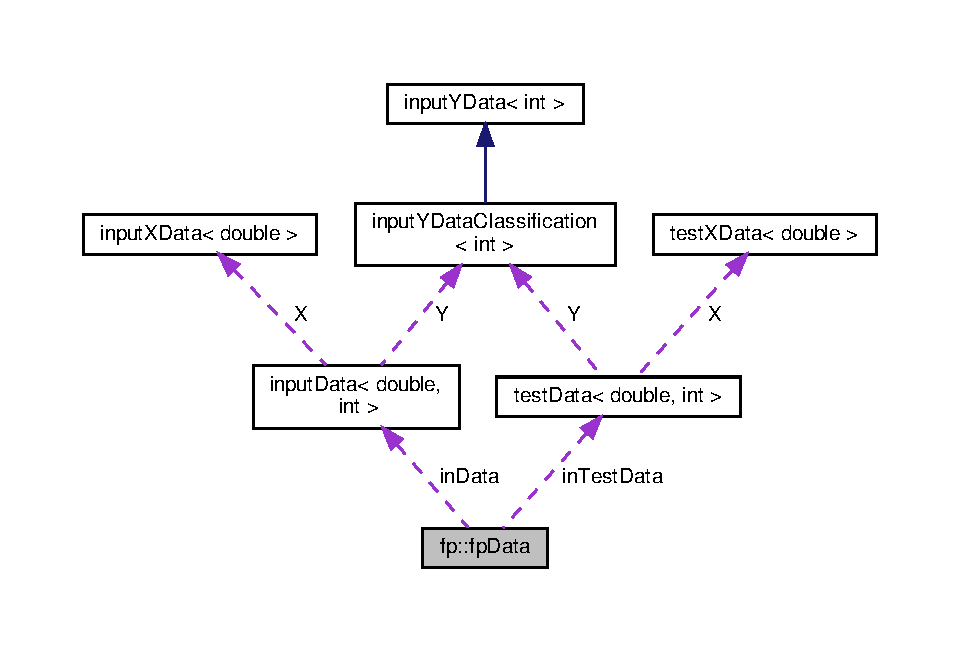
\includegraphics[width=350pt]{classfp_1_1fpData__coll__graph}
\end{center}
\end{figure}
\subsection*{Public Member Functions}
\begin{DoxyCompactItemize}
\item 
\hyperlink{classfp_1_1fpData_a0e111a379a969d2ff0b3e8c5911cf78a}{fp\+Data} ()
\item 
\hyperlink{classfp_1_1fpData_a62998c12f30ea88e6b3ea30b17d1a3e0}{$\sim$fp\+Data} ()
\item 
bool \hyperlink{classfp_1_1fpData_a2b4d9be328aaa7acf9a2561150da0402}{load\+Data\+From\+C\+SV} (\hyperlink{classfp_1_1fpInfo}{fp\+Info} \&settings)
\item 
void \hyperlink{classfp_1_1fpData_a91c727b1475eca340ca14c241b25c959}{fp\+Load\+Data} (\hyperlink{classfp_1_1fpInfo}{fp\+Info} \&settings)
\item 
void \hyperlink{classfp_1_1fpData_a44df119acad6c339966d67f2c634a369}{fp\+Delete\+Data} ()
\item 
int \hyperlink{classfp_1_1fpData_a7abfc93af30b7262d59b6d304796a09d}{return\+Num\+Classes} ()
\item 
int \hyperlink{classfp_1_1fpData_a95088e33b280e5c82b3543033d8852e1}{return\+Num\+Features} ()
\item 
int \hyperlink{classfp_1_1fpData_a9056a8c0e7e48fe9aa591269064ecc43}{return\+Num\+Observations} ()
\item 
int \hyperlink{classfp_1_1fpData_aac722f51424cb7f6ab7d89525f82cc72}{return\+Label} (int observation\+Number)
\item 
double \hyperlink{classfp_1_1fpData_a6b359086ec1e5c534095600e2ed5575f}{return\+Feature\+Val} (const int feature\+Number, const int observation\+Number)
\item 
void \hyperlink{classfp_1_1fpData_a3f9645ca93e9b64a788b3042e9e41fcc}{prefetch\+Feature\+Val} (const int feature\+Number, const int observation\+Number)
\item 
void \hyperlink{classfp_1_1fpData_ab48923d57206e17b88f0d89833051b43}{set\+Data\+Related\+Parameters} (\hyperlink{classfp_1_1fpInfo}{fp\+Info} \&settings)
\item 
int \hyperlink{classfp_1_1fpData_a9a115d29fafb6e5b941f4e0c860e65e7}{return\+Num\+Test\+Observations} ()
\item 
void \hyperlink{classfp_1_1fpData_ab60d2098334e253a0bf3115f029c1996}{set\+Test\+Data\+Related\+Parameters} (\hyperlink{classfp_1_1fpInfo}{fp\+Info} \&settings)
\item 
void \hyperlink{classfp_1_1fpData_a4b527bc84762c4708992b7fdce3d0602}{fp\+Load\+Test\+Data} (\hyperlink{classfp_1_1fpInfo}{fp\+Info} \&settings)
\item 
void \hyperlink{classfp_1_1fpData_a996eedfc5ffe559ce1f6061af1efc1db}{fp\+Delete\+Test\+Data} ()
\item 
int \hyperlink{classfp_1_1fpData_a50b6343c52560d1992de50e8cd6b1206}{return\+Test\+Label} (int observation\+Number)
\item 
double \hyperlink{classfp_1_1fpData_a42f76961f1649e329d654e9e1bb13fc6}{return\+Test\+Feature\+Val} (const int feature\+Number, const int observation\+Number)
\end{DoxyCompactItemize}
\subsection*{Protected Attributes}
\begin{DoxyCompactItemize}
\item 
\hyperlink{classfp_1_1inputData}{input\+Data}$<$ double, int $>$ $\ast$ \hyperlink{classfp_1_1fpData_a49d7c3f58bcf88843c25b1b0c9714ebe}{in\+Data}
\item 
\hyperlink{classfp_1_1testData}{test\+Data}$<$ double, int $>$ $\ast$ \hyperlink{classfp_1_1fpData_ad4f4dd3a8d15633b7f983932fa60bbad}{in\+Test\+Data}
\end{DoxyCompactItemize}


\subsection{Detailed Description}
\hyperlink{classfp_1_1fpData}{fp\+Data} holds both the training and test data. This data gets loaded from fp\+Dataset.

T\+O\+DO\+: This is not a good way to do this. There is nothing different from training data and test data. This is wrong. test data should be stored by observation whereas training data is stored by feature. 

Definition at line 19 of file fp\+Data.\+h.



\subsection{Constructor \& Destructor Documentation}
\mbox{\Hypertarget{classfp_1_1fpData_a0e111a379a969d2ff0b3e8c5911cf78a}\label{classfp_1_1fpData_a0e111a379a969d2ff0b3e8c5911cf78a}} 
\index{fp\+::fp\+Data@{fp\+::fp\+Data}!fp\+Data@{fp\+Data}}
\index{fp\+Data@{fp\+Data}!fp\+::fp\+Data@{fp\+::fp\+Data}}
\subsubsection{\texorpdfstring{fp\+Data()}{fpData()}}
{\footnotesize\ttfamily fp\+::fp\+Data\+::fp\+Data (\begin{DoxyParamCaption}{ }\end{DoxyParamCaption})\hspace{0.3cm}{\ttfamily [inline]}}



Definition at line 27 of file fp\+Data.\+h.


\begin{DoxyCode}
27                     \{
28             \}
\end{DoxyCode}
\mbox{\Hypertarget{classfp_1_1fpData_a62998c12f30ea88e6b3ea30b17d1a3e0}\label{classfp_1_1fpData_a62998c12f30ea88e6b3ea30b17d1a3e0}} 
\index{fp\+::fp\+Data@{fp\+::fp\+Data}!````~fp\+Data@{$\sim$fp\+Data}}
\index{````~fp\+Data@{$\sim$fp\+Data}!fp\+::fp\+Data@{fp\+::fp\+Data}}
\subsubsection{\texorpdfstring{$\sim$fp\+Data()}{~fpData()}}
{\footnotesize\ttfamily fp\+::fp\+Data\+::$\sim$fp\+Data (\begin{DoxyParamCaption}{ }\end{DoxyParamCaption})\hspace{0.3cm}{\ttfamily [inline]}}



Definition at line 30 of file fp\+Data.\+h.


\begin{DoxyCode}
30                      \{
31                 \textcolor{keywordflow}{if}(\hyperlink{classfp_1_1fpData_a49d7c3f58bcf88843c25b1b0c9714ebe}{inData} != NULL)\{
32                     \textcolor{keyword}{delete} \hyperlink{classfp_1_1fpData_a49d7c3f58bcf88843c25b1b0c9714ebe}{inData};
33                     \hyperlink{classfp_1_1fpData_a49d7c3f58bcf88843c25b1b0c9714ebe}{inData} = NULL;
34                 \}
35                 \textcolor{keywordflow}{if}(\hyperlink{classfp_1_1fpData_ad4f4dd3a8d15633b7f983932fa60bbad}{inTestData} != NULL)\{
36                     \textcolor{keyword}{delete} \hyperlink{classfp_1_1fpData_ad4f4dd3a8d15633b7f983932fa60bbad}{inTestData};
37                     \hyperlink{classfp_1_1fpData_ad4f4dd3a8d15633b7f983932fa60bbad}{inTestData} = NULL;
38                 \}
39             \}
\end{DoxyCode}


\subsection{Member Function Documentation}
\mbox{\Hypertarget{classfp_1_1fpData_a44df119acad6c339966d67f2c634a369}\label{classfp_1_1fpData_a44df119acad6c339966d67f2c634a369}} 
\index{fp\+::fp\+Data@{fp\+::fp\+Data}!fp\+Delete\+Data@{fp\+Delete\+Data}}
\index{fp\+Delete\+Data@{fp\+Delete\+Data}!fp\+::fp\+Data@{fp\+::fp\+Data}}
\subsubsection{\texorpdfstring{fp\+Delete\+Data()}{fpDeleteData()}}
{\footnotesize\ttfamily void fp\+::fp\+Data\+::fp\+Delete\+Data (\begin{DoxyParamCaption}{ }\end{DoxyParamCaption})\hspace{0.3cm}{\ttfamily [inline]}}



Definition at line 57 of file fp\+Data.\+h.


\begin{DoxyCode}
57                                \{
58                 \textcolor{keywordflow}{if}(\hyperlink{classfp_1_1fpData_a49d7c3f58bcf88843c25b1b0c9714ebe}{inData} != NULL)\{
59                     \textcolor{keyword}{delete} \hyperlink{classfp_1_1fpData_a49d7c3f58bcf88843c25b1b0c9714ebe}{inData};
60                     \hyperlink{classfp_1_1fpData_a49d7c3f58bcf88843c25b1b0c9714ebe}{inData} = NULL;
61                 \}\textcolor{keywordflow}{else} \{
62                     \textcolor{keywordflow}{throw} std::runtime\_error(\textcolor{stringliteral}{"Unable to delete data.  Data does not exist."} );
63                 \}
64             \}
\end{DoxyCode}
\mbox{\Hypertarget{classfp_1_1fpData_a996eedfc5ffe559ce1f6061af1efc1db}\label{classfp_1_1fpData_a996eedfc5ffe559ce1f6061af1efc1db}} 
\index{fp\+::fp\+Data@{fp\+::fp\+Data}!fp\+Delete\+Test\+Data@{fp\+Delete\+Test\+Data}}
\index{fp\+Delete\+Test\+Data@{fp\+Delete\+Test\+Data}!fp\+::fp\+Data@{fp\+::fp\+Data}}
\subsubsection{\texorpdfstring{fp\+Delete\+Test\+Data()}{fpDeleteTestData()}}
{\footnotesize\ttfamily void fp\+::fp\+Data\+::fp\+Delete\+Test\+Data (\begin{DoxyParamCaption}{ }\end{DoxyParamCaption})\hspace{0.3cm}{\ttfamily [inline]}}



Definition at line 119 of file fp\+Data.\+h.


\begin{DoxyCode}
119                                    \{
120                 \textcolor{keywordflow}{if}(\hyperlink{classfp_1_1fpData_ad4f4dd3a8d15633b7f983932fa60bbad}{inTestData} != NULL)\{
121                     \textcolor{keyword}{delete} \hyperlink{classfp_1_1fpData_ad4f4dd3a8d15633b7f983932fa60bbad}{inTestData};
122                     \hyperlink{classfp_1_1fpData_ad4f4dd3a8d15633b7f983932fa60bbad}{inTestData} = NULL;
123                 \}\textcolor{keywordflow}{else} \{
124                     \textcolor{keywordflow}{throw} std::runtime\_error(\textcolor{stringliteral}{"Unable to delete test data.  Test data does not exist."} );
125                 \}
126             \}
\end{DoxyCode}
\mbox{\Hypertarget{classfp_1_1fpData_a91c727b1475eca340ca14c241b25c959}\label{classfp_1_1fpData_a91c727b1475eca340ca14c241b25c959}} 
\index{fp\+::fp\+Data@{fp\+::fp\+Data}!fp\+Load\+Data@{fp\+Load\+Data}}
\index{fp\+Load\+Data@{fp\+Load\+Data}!fp\+::fp\+Data@{fp\+::fp\+Data}}
\subsubsection{\texorpdfstring{fp\+Load\+Data()}{fpLoadData()}}
{\footnotesize\ttfamily void fp\+::fp\+Data\+::fp\+Load\+Data (\begin{DoxyParamCaption}\item[{\hyperlink{classfp_1_1fpInfo}{fp\+Info} \&}]{settings }\end{DoxyParamCaption})\hspace{0.3cm}{\ttfamily [inline]}}



Definition at line 47 of file fp\+Data.\+h.


\begin{DoxyCode}
47                                              \{
48                 \textcolor{keywordflow}{if}(\hyperlink{classfp_1_1fpData_a2b4d9be328aaa7acf9a2561150da0402}{loadDataFromCSV}(settings))\{
49                     \hyperlink{classfp_1_1fpData_a49d7c3f58bcf88843c25b1b0c9714ebe}{inData} = \textcolor{keyword}{new} inputData<double,int>(settings.returnCSVFileName(), settings.
      returnColumnWithY());
50                 \}\textcolor{keywordflow}{else} \{
51                     \textcolor{keywordflow}{throw} std::runtime\_error(\textcolor{stringliteral}{"Unable to read data."} );
52                 \}
53                 \hyperlink{classfp_1_1fpData_ab48923d57206e17b88f0d89833051b43}{setDataRelatedParameters}(settings);
54             \}
\end{DoxyCode}
Here is the call graph for this function\+:
\nopagebreak
\begin{figure}[H]
\begin{center}
\leavevmode
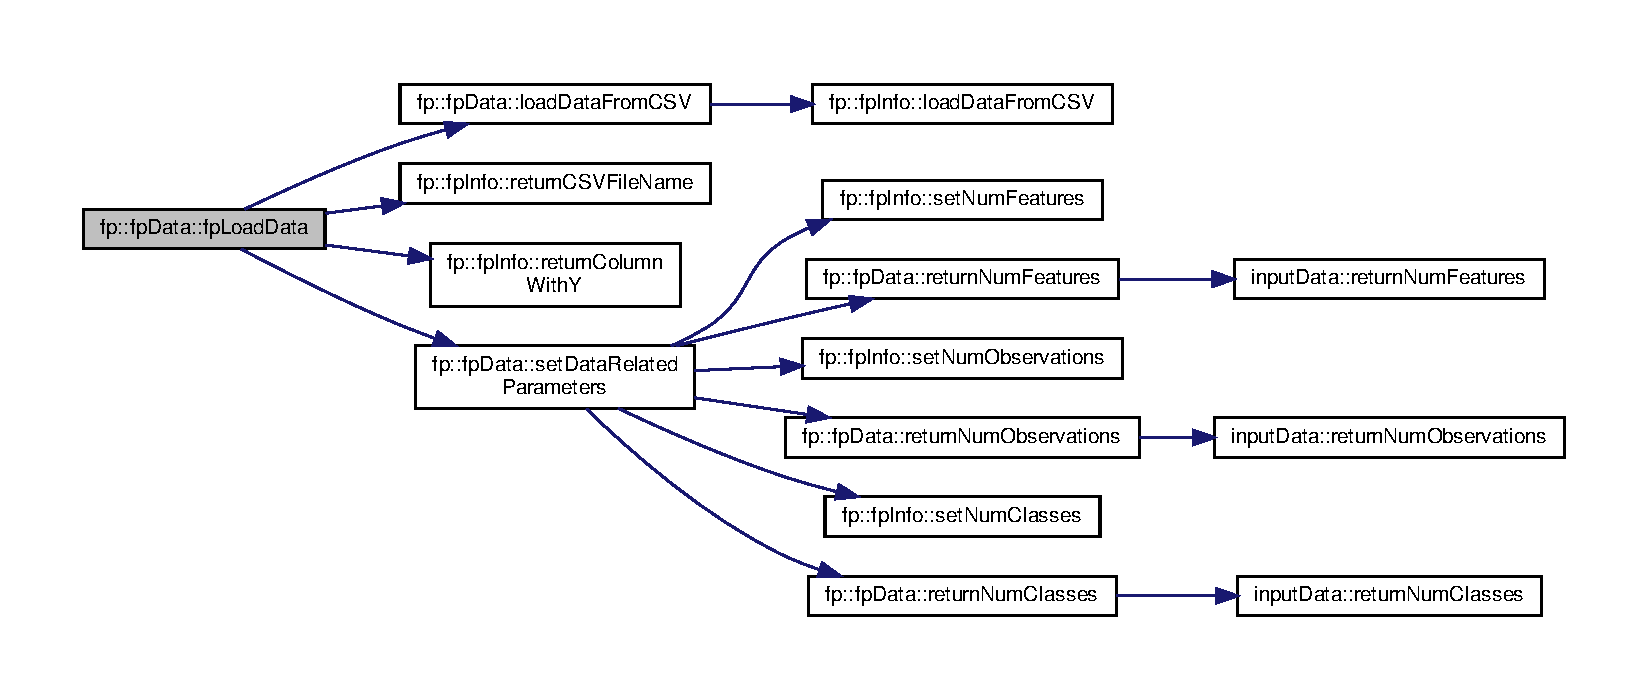
\includegraphics[width=350pt]{classfp_1_1fpData_a91c727b1475eca340ca14c241b25c959_cgraph}
\end{center}
\end{figure}
\mbox{\Hypertarget{classfp_1_1fpData_a4b527bc84762c4708992b7fdce3d0602}\label{classfp_1_1fpData_a4b527bc84762c4708992b7fdce3d0602}} 
\index{fp\+::fp\+Data@{fp\+::fp\+Data}!fp\+Load\+Test\+Data@{fp\+Load\+Test\+Data}}
\index{fp\+Load\+Test\+Data@{fp\+Load\+Test\+Data}!fp\+::fp\+Data@{fp\+::fp\+Data}}
\subsubsection{\texorpdfstring{fp\+Load\+Test\+Data()}{fpLoadTestData()}}
{\footnotesize\ttfamily void fp\+::fp\+Data\+::fp\+Load\+Test\+Data (\begin{DoxyParamCaption}\item[{\hyperlink{classfp_1_1fpInfo}{fp\+Info} \&}]{settings }\end{DoxyParamCaption})\hspace{0.3cm}{\ttfamily [inline]}}



Definition at line 109 of file fp\+Data.\+h.


\begin{DoxyCode}
109                                                  \{
110                 \textcolor{keywordflow}{if}(\hyperlink{classfp_1_1fpData_a2b4d9be328aaa7acf9a2561150da0402}{loadDataFromCSV}(settings))\{
111                     \hyperlink{classfp_1_1fpData_ad4f4dd3a8d15633b7f983932fa60bbad}{inTestData} = \textcolor{keyword}{new} testData<double,int>(settings.returnCSVFileName(), settings.
      returnColumnWithY());
112                 \}\textcolor{keywordflow}{else} \{
113                     \textcolor{keywordflow}{throw} std::runtime\_error(\textcolor{stringliteral}{"Unable to read test data."} );
114                 \}
115                 \hyperlink{classfp_1_1fpData_ab60d2098334e253a0bf3115f029c1996}{setTestDataRelatedParameters}(settings);
116             \}
\end{DoxyCode}
Here is the call graph for this function\+:
\nopagebreak
\begin{figure}[H]
\begin{center}
\leavevmode
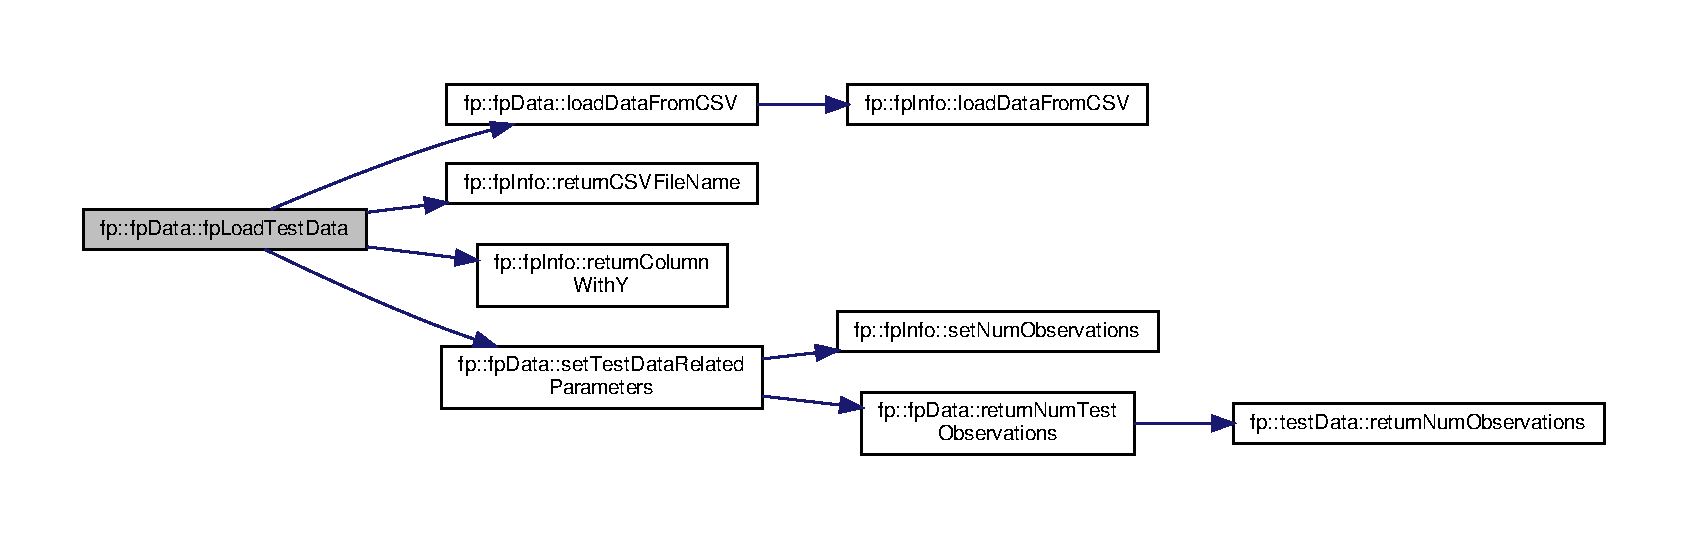
\includegraphics[width=350pt]{classfp_1_1fpData_a4b527bc84762c4708992b7fdce3d0602_cgraph}
\end{center}
\end{figure}
\mbox{\Hypertarget{classfp_1_1fpData_a2b4d9be328aaa7acf9a2561150da0402}\label{classfp_1_1fpData_a2b4d9be328aaa7acf9a2561150da0402}} 
\index{fp\+::fp\+Data@{fp\+::fp\+Data}!load\+Data\+From\+C\+SV@{load\+Data\+From\+C\+SV}}
\index{load\+Data\+From\+C\+SV@{load\+Data\+From\+C\+SV}!fp\+::fp\+Data@{fp\+::fp\+Data}}
\subsubsection{\texorpdfstring{load\+Data\+From\+C\+S\+V()}{loadDataFromCSV()}}
{\footnotesize\ttfamily bool fp\+::fp\+Data\+::load\+Data\+From\+C\+SV (\begin{DoxyParamCaption}\item[{\hyperlink{classfp_1_1fpInfo}{fp\+Info} \&}]{settings }\end{DoxyParamCaption})\hspace{0.3cm}{\ttfamily [inline]}}



Definition at line 42 of file fp\+Data.\+h.


\begin{DoxyCode}
42                                                          \{
43                 \textcolor{keywordflow}{return} settings.loadDataFromCSV();
44             \}
\end{DoxyCode}
Here is the call graph for this function\+:\nopagebreak
\begin{figure}[H]
\begin{center}
\leavevmode
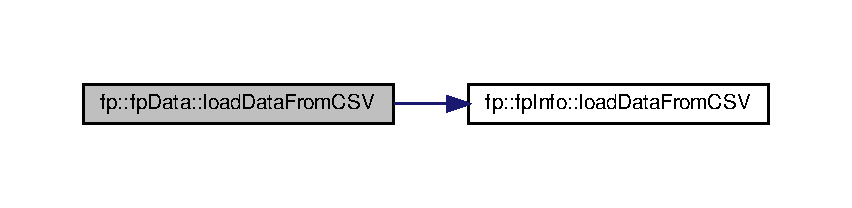
\includegraphics[width=350pt]{classfp_1_1fpData_a2b4d9be328aaa7acf9a2561150da0402_cgraph}
\end{center}
\end{figure}
\mbox{\Hypertarget{classfp_1_1fpData_a3f9645ca93e9b64a788b3042e9e41fcc}\label{classfp_1_1fpData_a3f9645ca93e9b64a788b3042e9e41fcc}} 
\index{fp\+::fp\+Data@{fp\+::fp\+Data}!prefetch\+Feature\+Val@{prefetch\+Feature\+Val}}
\index{prefetch\+Feature\+Val@{prefetch\+Feature\+Val}!fp\+::fp\+Data@{fp\+::fp\+Data}}
\subsubsection{\texorpdfstring{prefetch\+Feature\+Val()}{prefetchFeatureVal()}}
{\footnotesize\ttfamily void fp\+::fp\+Data\+::prefetch\+Feature\+Val (\begin{DoxyParamCaption}\item[{const int}]{feature\+Number,  }\item[{const int}]{observation\+Number }\end{DoxyParamCaption})\hspace{0.3cm}{\ttfamily [inline]}}



Definition at line 88 of file fp\+Data.\+h.


\begin{DoxyCode}
88                                                                                                 \{
89                 \hyperlink{classfp_1_1fpData_a49d7c3f58bcf88843c25b1b0c9714ebe}{inData}->\hyperlink{classfp_1_1inputData_a348baff7c24d263bb24185dbaa19d455}{prefetchFeatureValue}(featureNumber, observationNumber);
90             \}
\end{DoxyCode}
Here is the call graph for this function\+:
\nopagebreak
\begin{figure}[H]
\begin{center}
\leavevmode
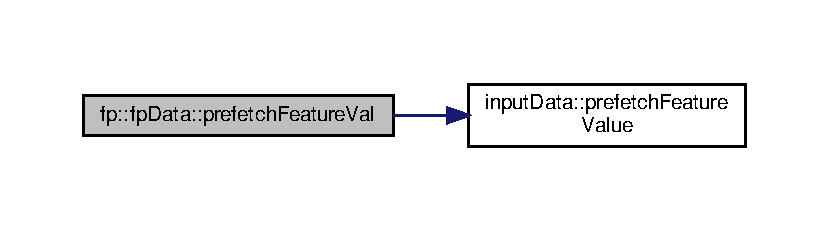
\includegraphics[width=350pt]{classfp_1_1fpData_a3f9645ca93e9b64a788b3042e9e41fcc_cgraph}
\end{center}
\end{figure}
\mbox{\Hypertarget{classfp_1_1fpData_a6b359086ec1e5c534095600e2ed5575f}\label{classfp_1_1fpData_a6b359086ec1e5c534095600e2ed5575f}} 
\index{fp\+::fp\+Data@{fp\+::fp\+Data}!return\+Feature\+Val@{return\+Feature\+Val}}
\index{return\+Feature\+Val@{return\+Feature\+Val}!fp\+::fp\+Data@{fp\+::fp\+Data}}
\subsubsection{\texorpdfstring{return\+Feature\+Val()}{returnFeatureVal()}}
{\footnotesize\ttfamily double fp\+::fp\+Data\+::return\+Feature\+Val (\begin{DoxyParamCaption}\item[{const int}]{feature\+Number,  }\item[{const int}]{observation\+Number }\end{DoxyParamCaption})\hspace{0.3cm}{\ttfamily [inline]}}



Definition at line 84 of file fp\+Data.\+h.


\begin{DoxyCode}
84                                                                                                 \{
85                 \textcolor{keywordflow}{return} \hyperlink{classfp_1_1fpData_a49d7c3f58bcf88843c25b1b0c9714ebe}{inData}->\hyperlink{classfp_1_1inputData_af52ac3512ee8f6e973799e024ddbf629}{returnFeatureValue}(featureNumber, observationNumber)
      ;
86             \}
\end{DoxyCode}
Here is the call graph for this function\+:
\nopagebreak
\begin{figure}[H]
\begin{center}
\leavevmode
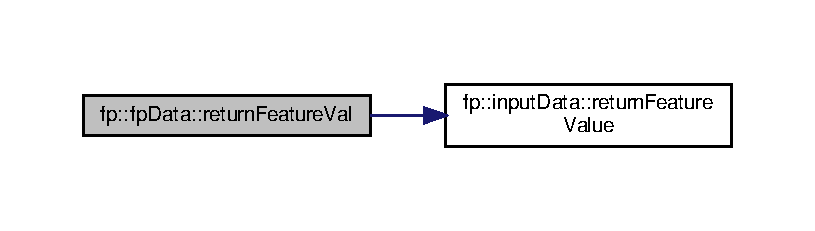
\includegraphics[width=350pt]{classfp_1_1fpData_a6b359086ec1e5c534095600e2ed5575f_cgraph}
\end{center}
\end{figure}
\mbox{\Hypertarget{classfp_1_1fpData_aac722f51424cb7f6ab7d89525f82cc72}\label{classfp_1_1fpData_aac722f51424cb7f6ab7d89525f82cc72}} 
\index{fp\+::fp\+Data@{fp\+::fp\+Data}!return\+Label@{return\+Label}}
\index{return\+Label@{return\+Label}!fp\+::fp\+Data@{fp\+::fp\+Data}}
\subsubsection{\texorpdfstring{return\+Label()}{returnLabel()}}
{\footnotesize\ttfamily int fp\+::fp\+Data\+::return\+Label (\begin{DoxyParamCaption}\item[{int}]{observation\+Number }\end{DoxyParamCaption})\hspace{0.3cm}{\ttfamily [inline]}}



Definition at line 80 of file fp\+Data.\+h.


\begin{DoxyCode}
80                                                          \{
81                 \textcolor{keywordflow}{return} \hyperlink{classfp_1_1fpData_a49d7c3f58bcf88843c25b1b0c9714ebe}{inData}->\hyperlink{classfp_1_1inputData_a0a767252e950159110d3f2a0c74064ec}{returnClassOfObservation}(observationNumber);
82             \}
\end{DoxyCode}
Here is the call graph for this function\+:
\nopagebreak
\begin{figure}[H]
\begin{center}
\leavevmode
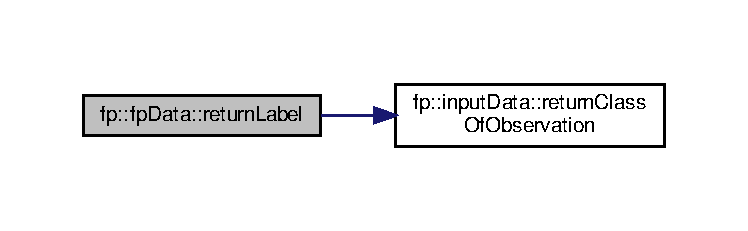
\includegraphics[width=350pt]{classfp_1_1fpData_aac722f51424cb7f6ab7d89525f82cc72_cgraph}
\end{center}
\end{figure}
\mbox{\Hypertarget{classfp_1_1fpData_a7abfc93af30b7262d59b6d304796a09d}\label{classfp_1_1fpData_a7abfc93af30b7262d59b6d304796a09d}} 
\index{fp\+::fp\+Data@{fp\+::fp\+Data}!return\+Num\+Classes@{return\+Num\+Classes}}
\index{return\+Num\+Classes@{return\+Num\+Classes}!fp\+::fp\+Data@{fp\+::fp\+Data}}
\subsubsection{\texorpdfstring{return\+Num\+Classes()}{returnNumClasses()}}
{\footnotesize\ttfamily int fp\+::fp\+Data\+::return\+Num\+Classes (\begin{DoxyParamCaption}{ }\end{DoxyParamCaption})\hspace{0.3cm}{\ttfamily [inline]}}



Definition at line 67 of file fp\+Data.\+h.


\begin{DoxyCode}
67                                          \{
68                 \textcolor{keywordflow}{return} \hyperlink{classfp_1_1fpData_a49d7c3f58bcf88843c25b1b0c9714ebe}{inData}->\hyperlink{classfp_1_1inputData_a1e775e3744cb3bacb1a6776054aabe4f}{returnNumClasses}();
69             \}
\end{DoxyCode}
Here is the call graph for this function\+:
\nopagebreak
\begin{figure}[H]
\begin{center}
\leavevmode
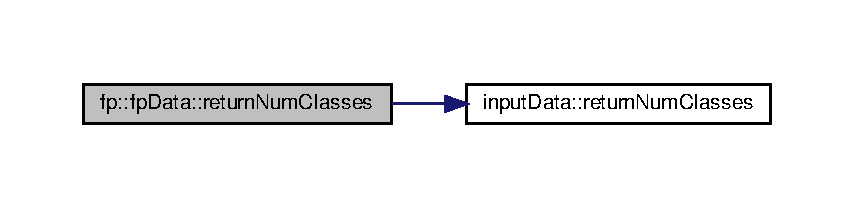
\includegraphics[width=350pt]{classfp_1_1fpData_a7abfc93af30b7262d59b6d304796a09d_cgraph}
\end{center}
\end{figure}
\mbox{\Hypertarget{classfp_1_1fpData_a95088e33b280e5c82b3543033d8852e1}\label{classfp_1_1fpData_a95088e33b280e5c82b3543033d8852e1}} 
\index{fp\+::fp\+Data@{fp\+::fp\+Data}!return\+Num\+Features@{return\+Num\+Features}}
\index{return\+Num\+Features@{return\+Num\+Features}!fp\+::fp\+Data@{fp\+::fp\+Data}}
\subsubsection{\texorpdfstring{return\+Num\+Features()}{returnNumFeatures()}}
{\footnotesize\ttfamily int fp\+::fp\+Data\+::return\+Num\+Features (\begin{DoxyParamCaption}{ }\end{DoxyParamCaption})\hspace{0.3cm}{\ttfamily [inline]}}



Definition at line 72 of file fp\+Data.\+h.


\begin{DoxyCode}
72                                           \{
73                 \textcolor{keywordflow}{return} \hyperlink{classfp_1_1fpData_a49d7c3f58bcf88843c25b1b0c9714ebe}{inData}->\hyperlink{classfp_1_1inputData_ae9362286ea7706a8b0d91ba96e9ad478}{returnNumFeatures}();
74             \}
\end{DoxyCode}
Here is the call graph for this function\+:
\nopagebreak
\begin{figure}[H]
\begin{center}
\leavevmode
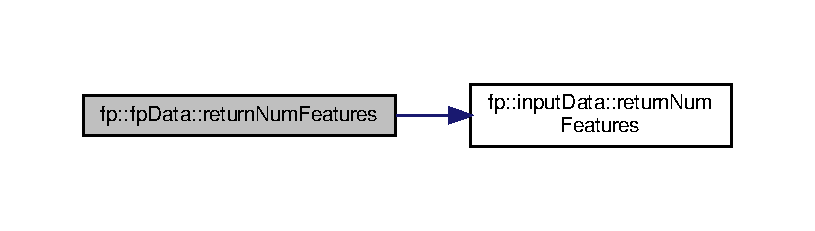
\includegraphics[width=350pt]{classfp_1_1fpData_a95088e33b280e5c82b3543033d8852e1_cgraph}
\end{center}
\end{figure}
\mbox{\Hypertarget{classfp_1_1fpData_a9056a8c0e7e48fe9aa591269064ecc43}\label{classfp_1_1fpData_a9056a8c0e7e48fe9aa591269064ecc43}} 
\index{fp\+::fp\+Data@{fp\+::fp\+Data}!return\+Num\+Observations@{return\+Num\+Observations}}
\index{return\+Num\+Observations@{return\+Num\+Observations}!fp\+::fp\+Data@{fp\+::fp\+Data}}
\subsubsection{\texorpdfstring{return\+Num\+Observations()}{returnNumObservations()}}
{\footnotesize\ttfamily int fp\+::fp\+Data\+::return\+Num\+Observations (\begin{DoxyParamCaption}{ }\end{DoxyParamCaption})\hspace{0.3cm}{\ttfamily [inline]}}



Definition at line 76 of file fp\+Data.\+h.


\begin{DoxyCode}
76                                               \{
77                 \textcolor{keywordflow}{return} \hyperlink{classfp_1_1fpData_a49d7c3f58bcf88843c25b1b0c9714ebe}{inData}->\hyperlink{classfp_1_1inputData_af7dc02941195e025d1d89c882096027d}{returnNumObservations}();
78             \}
\end{DoxyCode}
Here is the call graph for this function\+:
\nopagebreak
\begin{figure}[H]
\begin{center}
\leavevmode
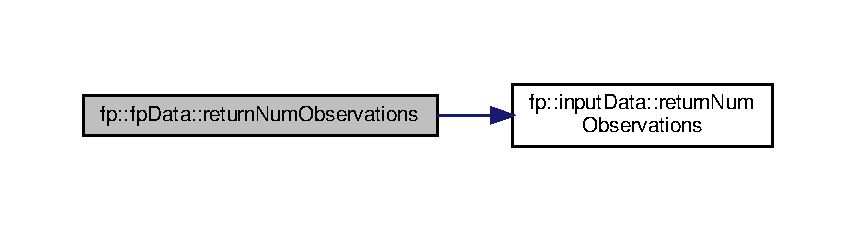
\includegraphics[width=350pt]{classfp_1_1fpData_a9056a8c0e7e48fe9aa591269064ecc43_cgraph}
\end{center}
\end{figure}
\mbox{\Hypertarget{classfp_1_1fpData_a9a115d29fafb6e5b941f4e0c860e65e7}\label{classfp_1_1fpData_a9a115d29fafb6e5b941f4e0c860e65e7}} 
\index{fp\+::fp\+Data@{fp\+::fp\+Data}!return\+Num\+Test\+Observations@{return\+Num\+Test\+Observations}}
\index{return\+Num\+Test\+Observations@{return\+Num\+Test\+Observations}!fp\+::fp\+Data@{fp\+::fp\+Data}}
\subsubsection{\texorpdfstring{return\+Num\+Test\+Observations()}{returnNumTestObservations()}}
{\footnotesize\ttfamily int fp\+::fp\+Data\+::return\+Num\+Test\+Observations (\begin{DoxyParamCaption}{ }\end{DoxyParamCaption})\hspace{0.3cm}{\ttfamily [inline]}}



Definition at line 101 of file fp\+Data.\+h.


\begin{DoxyCode}
101                                                   \{
102                 \textcolor{keywordflow}{return} \hyperlink{classfp_1_1fpData_ad4f4dd3a8d15633b7f983932fa60bbad}{inTestData}->\hyperlink{classfp_1_1testData_af9dd7a4aa116d99a11838a02f2154c08}{returnNumObservations}();
103             \}
\end{DoxyCode}
Here is the call graph for this function\+:
\nopagebreak
\begin{figure}[H]
\begin{center}
\leavevmode
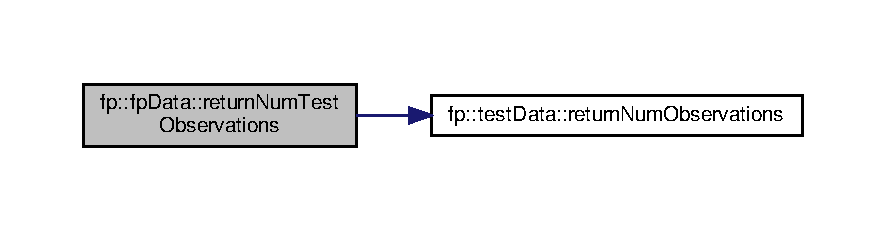
\includegraphics[width=350pt]{classfp_1_1fpData_a9a115d29fafb6e5b941f4e0c860e65e7_cgraph}
\end{center}
\end{figure}
\mbox{\Hypertarget{classfp_1_1fpData_a42f76961f1649e329d654e9e1bb13fc6}\label{classfp_1_1fpData_a42f76961f1649e329d654e9e1bb13fc6}} 
\index{fp\+::fp\+Data@{fp\+::fp\+Data}!return\+Test\+Feature\+Val@{return\+Test\+Feature\+Val}}
\index{return\+Test\+Feature\+Val@{return\+Test\+Feature\+Val}!fp\+::fp\+Data@{fp\+::fp\+Data}}
\subsubsection{\texorpdfstring{return\+Test\+Feature\+Val()}{returnTestFeatureVal()}}
{\footnotesize\ttfamily double fp\+::fp\+Data\+::return\+Test\+Feature\+Val (\begin{DoxyParamCaption}\item[{const int}]{feature\+Number,  }\item[{const int}]{observation\+Number }\end{DoxyParamCaption})\hspace{0.3cm}{\ttfamily [inline]}}



Definition at line 132 of file fp\+Data.\+h.


\begin{DoxyCode}
132                                                                                                     \{
133                 \textcolor{keywordflow}{return} \hyperlink{classfp_1_1fpData_ad4f4dd3a8d15633b7f983932fa60bbad}{inTestData}->\hyperlink{classfp_1_1testData_a0c49c5fc2f1bf3fc39c7d55413cddabf}{returnFeatureValue}(featureNumber, 
      observationNumber);
134             \}
\end{DoxyCode}
Here is the call graph for this function\+:
\nopagebreak
\begin{figure}[H]
\begin{center}
\leavevmode
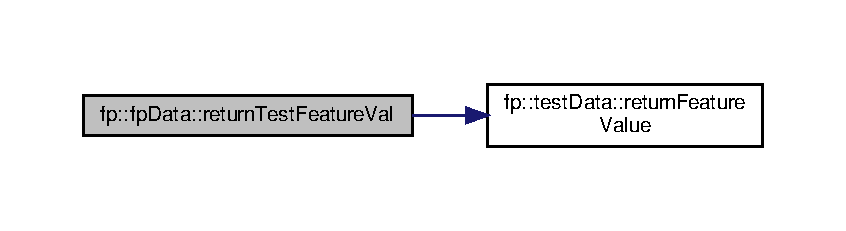
\includegraphics[width=350pt]{classfp_1_1fpData_a42f76961f1649e329d654e9e1bb13fc6_cgraph}
\end{center}
\end{figure}
\mbox{\Hypertarget{classfp_1_1fpData_a50b6343c52560d1992de50e8cd6b1206}\label{classfp_1_1fpData_a50b6343c52560d1992de50e8cd6b1206}} 
\index{fp\+::fp\+Data@{fp\+::fp\+Data}!return\+Test\+Label@{return\+Test\+Label}}
\index{return\+Test\+Label@{return\+Test\+Label}!fp\+::fp\+Data@{fp\+::fp\+Data}}
\subsubsection{\texorpdfstring{return\+Test\+Label()}{returnTestLabel()}}
{\footnotesize\ttfamily int fp\+::fp\+Data\+::return\+Test\+Label (\begin{DoxyParamCaption}\item[{int}]{observation\+Number }\end{DoxyParamCaption})\hspace{0.3cm}{\ttfamily [inline]}}



Definition at line 129 of file fp\+Data.\+h.


\begin{DoxyCode}
129                                                              \{
130                 \textcolor{keywordflow}{return} \hyperlink{classfp_1_1fpData_ad4f4dd3a8d15633b7f983932fa60bbad}{inTestData}->\hyperlink{classfp_1_1testData_a3a964b20b07dd4b49e958fdde93ebc59}{returnClassOfObservation}(
      observationNumber);
131             \}
\end{DoxyCode}
Here is the call graph for this function\+:
\nopagebreak
\begin{figure}[H]
\begin{center}
\leavevmode
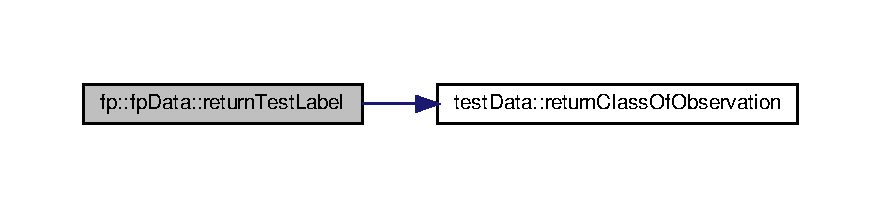
\includegraphics[width=350pt]{classfp_1_1fpData_a50b6343c52560d1992de50e8cd6b1206_cgraph}
\end{center}
\end{figure}
\mbox{\Hypertarget{classfp_1_1fpData_ab48923d57206e17b88f0d89833051b43}\label{classfp_1_1fpData_ab48923d57206e17b88f0d89833051b43}} 
\index{fp\+::fp\+Data@{fp\+::fp\+Data}!set\+Data\+Related\+Parameters@{set\+Data\+Related\+Parameters}}
\index{set\+Data\+Related\+Parameters@{set\+Data\+Related\+Parameters}!fp\+::fp\+Data@{fp\+::fp\+Data}}
\subsubsection{\texorpdfstring{set\+Data\+Related\+Parameters()}{setDataRelatedParameters()}}
{\footnotesize\ttfamily void fp\+::fp\+Data\+::set\+Data\+Related\+Parameters (\begin{DoxyParamCaption}\item[{\hyperlink{classfp_1_1fpInfo}{fp\+Info} \&}]{settings }\end{DoxyParamCaption})\hspace{0.3cm}{\ttfamily [inline]}}



Definition at line 94 of file fp\+Data.\+h.


\begin{DoxyCode}
94                                                                   \{
95                 settings.setNumFeatures(this->\hyperlink{classfp_1_1fpData_a95088e33b280e5c82b3543033d8852e1}{returnNumFeatures}());
96                 settings.setNumObservations(this->\hyperlink{classfp_1_1fpData_a9056a8c0e7e48fe9aa591269064ecc43}{returnNumObservations}());
97                 settings.setNumClasses(this->\hyperlink{classfp_1_1fpData_a7abfc93af30b7262d59b6d304796a09d}{returnNumClasses}());
98             \}
\end{DoxyCode}
Here is the call graph for this function\+:
\nopagebreak
\begin{figure}[H]
\begin{center}
\leavevmode
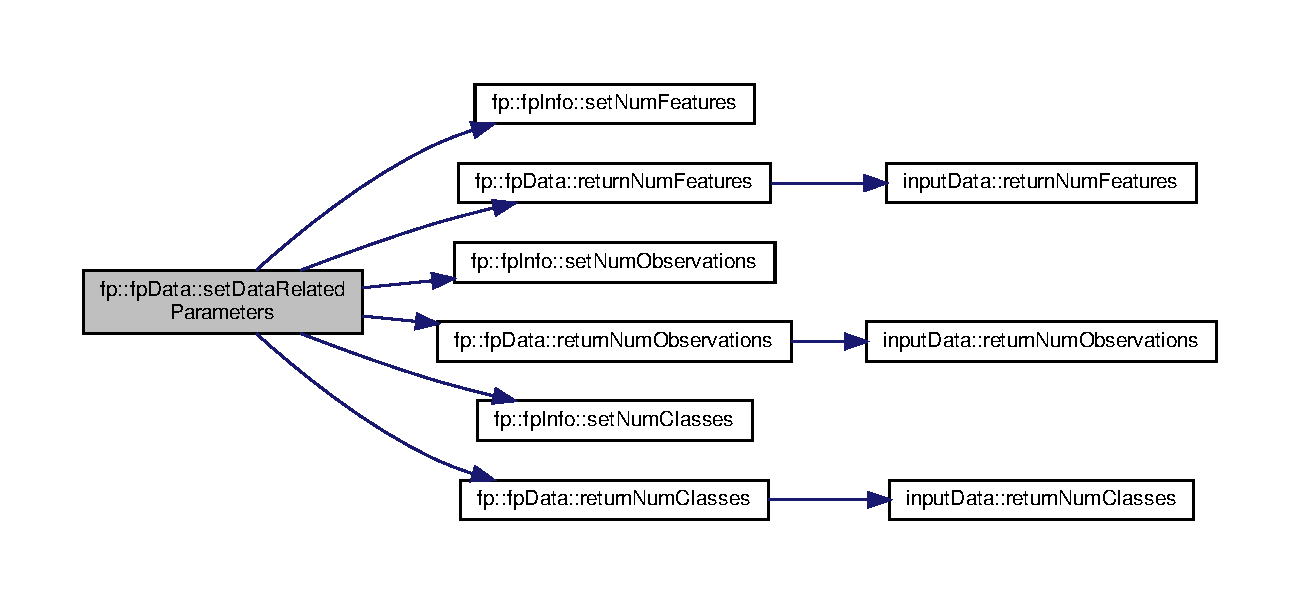
\includegraphics[width=350pt]{classfp_1_1fpData_ab48923d57206e17b88f0d89833051b43_cgraph}
\end{center}
\end{figure}
\mbox{\Hypertarget{classfp_1_1fpData_ab60d2098334e253a0bf3115f029c1996}\label{classfp_1_1fpData_ab60d2098334e253a0bf3115f029c1996}} 
\index{fp\+::fp\+Data@{fp\+::fp\+Data}!set\+Test\+Data\+Related\+Parameters@{set\+Test\+Data\+Related\+Parameters}}
\index{set\+Test\+Data\+Related\+Parameters@{set\+Test\+Data\+Related\+Parameters}!fp\+::fp\+Data@{fp\+::fp\+Data}}
\subsubsection{\texorpdfstring{set\+Test\+Data\+Related\+Parameters()}{setTestDataRelatedParameters()}}
{\footnotesize\ttfamily void fp\+::fp\+Data\+::set\+Test\+Data\+Related\+Parameters (\begin{DoxyParamCaption}\item[{\hyperlink{classfp_1_1fpInfo}{fp\+Info} \&}]{settings }\end{DoxyParamCaption})\hspace{0.3cm}{\ttfamily [inline]}}



Definition at line 105 of file fp\+Data.\+h.


\begin{DoxyCode}
105                                                                       \{
106                 settings.setNumObservations(this->\hyperlink{classfp_1_1fpData_a9a115d29fafb6e5b941f4e0c860e65e7}{returnNumTestObservations}());
107             \}
\end{DoxyCode}
Here is the call graph for this function\+:
\nopagebreak
\begin{figure}[H]
\begin{center}
\leavevmode
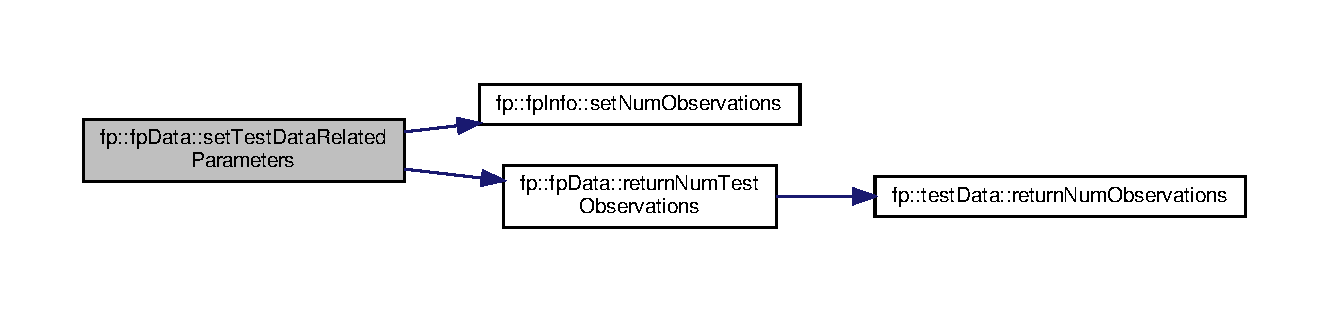
\includegraphics[width=350pt]{classfp_1_1fpData_ab60d2098334e253a0bf3115f029c1996_cgraph}
\end{center}
\end{figure}


\subsection{Member Data Documentation}
\mbox{\Hypertarget{classfp_1_1fpData_a49d7c3f58bcf88843c25b1b0c9714ebe}\label{classfp_1_1fpData_a49d7c3f58bcf88843c25b1b0c9714ebe}} 
\index{fp\+::fp\+Data@{fp\+::fp\+Data}!in\+Data@{in\+Data}}
\index{in\+Data@{in\+Data}!fp\+::fp\+Data@{fp\+::fp\+Data}}
\subsubsection{\texorpdfstring{in\+Data}{inData}}
{\footnotesize\ttfamily \hyperlink{classfp_1_1inputData}{input\+Data}$<$double, int$>$$\ast$ fp\+::fp\+Data\+::in\+Data\hspace{0.3cm}{\ttfamily [protected]}}



Definition at line 22 of file fp\+Data.\+h.

\mbox{\Hypertarget{classfp_1_1fpData_ad4f4dd3a8d15633b7f983932fa60bbad}\label{classfp_1_1fpData_ad4f4dd3a8d15633b7f983932fa60bbad}} 
\index{fp\+::fp\+Data@{fp\+::fp\+Data}!in\+Test\+Data@{in\+Test\+Data}}
\index{in\+Test\+Data@{in\+Test\+Data}!fp\+::fp\+Data@{fp\+::fp\+Data}}
\subsubsection{\texorpdfstring{in\+Test\+Data}{inTestData}}
{\footnotesize\ttfamily \hyperlink{classfp_1_1testData}{test\+Data}$<$double, int$>$$\ast$ fp\+::fp\+Data\+::in\+Test\+Data\hspace{0.3cm}{\ttfamily [protected]}}



Definition at line 23 of file fp\+Data.\+h.



The documentation for this class was generated from the following file\+:\begin{DoxyCompactItemize}
\item 
src/fp\+Singleton/\hyperlink{fpData_8h}{fp\+Data.\+h}\end{DoxyCompactItemize}

\hypertarget{classfp_1_1fpDisplayProgress}{}\section{fp\+:\+:fp\+Display\+Progress Class Reference}
\label{classfp_1_1fpDisplayProgress}\index{fp\+::fp\+Display\+Progress@{fp\+::fp\+Display\+Progress}}


{\ttfamily \#include $<$display\+Progress.\+h$>$}

\subsection*{Public Member Functions}
\begin{DoxyCompactItemize}
\item 
void \hyperlink{classfp_1_1fpDisplayProgress_adf5b2e390618d63eccb6de3b00eb857b}{display\+Progress} (int tree\+Num)
\end{DoxyCompactItemize}


\subsection{Detailed Description}


Definition at line 35 of file display\+Progress.\+h.



\subsection{Member Function Documentation}
\mbox{\Hypertarget{classfp_1_1fpDisplayProgress_adf5b2e390618d63eccb6de3b00eb857b}\label{classfp_1_1fpDisplayProgress_adf5b2e390618d63eccb6de3b00eb857b}} 
\index{fp\+::fp\+Display\+Progress@{fp\+::fp\+Display\+Progress}!display\+Progress@{display\+Progress}}
\index{display\+Progress@{display\+Progress}!fp\+::fp\+Display\+Progress@{fp\+::fp\+Display\+Progress}}
\subsubsection{\texorpdfstring{display\+Progress()}{displayProgress()}}
{\footnotesize\ttfamily void fp\+::fp\+Display\+Progress\+::display\+Progress (\begin{DoxyParamCaption}\item[{int}]{tree\+Num }\end{DoxyParamCaption})\hspace{0.3cm}{\ttfamily [inline]}}



Definition at line 37 of file display\+Progress.\+h.


\begin{DoxyCode}
37                                                  \{ 
38             \textcolor{keyword}{static} fpDisplayProgressStaticStore staticPrint;
39             staticPrint.print(treeNum); \} 
\end{DoxyCode}
Here is the call graph for this function\+:
\nopagebreak
\begin{figure}[H]
\begin{center}
\leavevmode
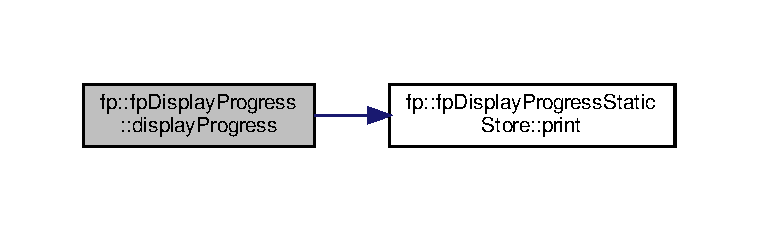
\includegraphics[width=350pt]{classfp_1_1fpDisplayProgress_adf5b2e390618d63eccb6de3b00eb857b_cgraph}
\end{center}
\end{figure}


The documentation for this class was generated from the following file\+:\begin{DoxyCompactItemize}
\item 
src/base\+Functions/\hyperlink{displayProgress_8h}{display\+Progress.\+h}\end{DoxyCompactItemize}

\hypertarget{classfp_1_1fpDisplayProgressStaticStore}{}\section{fp\+:\+:fp\+Display\+Progress\+Static\+Store Class Reference}
\label{classfp_1_1fpDisplayProgressStaticStore}\index{fp\+::fp\+Display\+Progress\+Static\+Store@{fp\+::fp\+Display\+Progress\+Static\+Store}}


{\ttfamily \#include $<$display\+Progress.\+h$>$}

\subsection*{Public Member Functions}
\begin{DoxyCompactItemize}
\item 
\hyperlink{classfp_1_1fpDisplayProgressStaticStore_a31330f7f864dff5ba94f5c59439b016f}{fp\+Display\+Progress\+Static\+Store} ()
\item 
void \hyperlink{classfp_1_1fpDisplayProgressStaticStore_a9b2ab53929032183e681157515cf5313}{print} (int i)
\end{DoxyCompactItemize}
\subsection*{Private Attributes}
\begin{DoxyCompactItemize}
\item 
std\+::chrono\+::time\+\_\+point$<$ system\+\_\+clock $>$ \hyperlink{classfp_1_1fpDisplayProgressStaticStore_aa602428554cc8543ec40617ffacd531d}{start\+Time}
\item 
std\+::chrono\+::time\+\_\+point$<$ system\+\_\+clock $>$ \hyperlink{classfp_1_1fpDisplayProgressStaticStore_a7af621498c605e7955b9f1bb2abdb5a4}{stop\+Time}
\item 
std\+::chrono\+::seconds \hyperlink{classfp_1_1fpDisplayProgressStaticStore_a9765e1784e83522a0b842d342e479816}{diff\+Seconds}
\end{DoxyCompactItemize}


\subsection{Detailed Description}


Definition at line 10 of file display\+Progress.\+h.



\subsection{Constructor \& Destructor Documentation}
\mbox{\Hypertarget{classfp_1_1fpDisplayProgressStaticStore_a31330f7f864dff5ba94f5c59439b016f}\label{classfp_1_1fpDisplayProgressStaticStore_a31330f7f864dff5ba94f5c59439b016f}} 
\index{fp\+::fp\+Display\+Progress\+Static\+Store@{fp\+::fp\+Display\+Progress\+Static\+Store}!fp\+Display\+Progress\+Static\+Store@{fp\+Display\+Progress\+Static\+Store}}
\index{fp\+Display\+Progress\+Static\+Store@{fp\+Display\+Progress\+Static\+Store}!fp\+::fp\+Display\+Progress\+Static\+Store@{fp\+::fp\+Display\+Progress\+Static\+Store}}
\subsubsection{\texorpdfstring{fp\+Display\+Progress\+Static\+Store()}{fpDisplayProgressStaticStore()}}
{\footnotesize\ttfamily fp\+::fp\+Display\+Progress\+Static\+Store\+::fp\+Display\+Progress\+Static\+Store (\begin{DoxyParamCaption}{ }\end{DoxyParamCaption})\hspace{0.3cm}{\ttfamily [inline]}}



Definition at line 18 of file display\+Progress.\+h.


\begin{DoxyCode}
18                                           \{
19                 \hyperlink{classfp_1_1fpDisplayProgressStaticStore_aa602428554cc8543ec40617ffacd531d}{startTime} = std::chrono::system\_clock::now();
20                 std::cout << \textcolor{stringliteral}{"starting tree 1"} << std::flush;
21             \}
\end{DoxyCode}


\subsection{Member Function Documentation}
\mbox{\Hypertarget{classfp_1_1fpDisplayProgressStaticStore_a9b2ab53929032183e681157515cf5313}\label{classfp_1_1fpDisplayProgressStaticStore_a9b2ab53929032183e681157515cf5313}} 
\index{fp\+::fp\+Display\+Progress\+Static\+Store@{fp\+::fp\+Display\+Progress\+Static\+Store}!print@{print}}
\index{print@{print}!fp\+::fp\+Display\+Progress\+Static\+Store@{fp\+::fp\+Display\+Progress\+Static\+Store}}
\subsubsection{\texorpdfstring{print()}{print()}}
{\footnotesize\ttfamily void fp\+::fp\+Display\+Progress\+Static\+Store\+::print (\begin{DoxyParamCaption}\item[{int}]{i }\end{DoxyParamCaption})\hspace{0.3cm}{\ttfamily [inline]}}



Definition at line 23 of file display\+Progress.\+h.


\begin{DoxyCode}
23                                     \{
24             std::chrono::seconds updateTime(10);
25                 \hyperlink{classfp_1_1fpDisplayProgressStaticStore_a7af621498c605e7955b9f1bb2abdb5a4}{stopTime} = std::chrono::high\_resolution\_clock::now();
26                 \hyperlink{classfp_1_1fpDisplayProgressStaticStore_a9765e1784e83522a0b842d342e479816}{diffSeconds} =    std::chrono::duration\_cast<std::chrono::seconds>(
      \hyperlink{classfp_1_1fpDisplayProgressStaticStore_a7af621498c605e7955b9f1bb2abdb5a4}{stopTime} - \hyperlink{classfp_1_1fpDisplayProgressStaticStore_aa602428554cc8543ec40617ffacd531d}{startTime});
27                 \textcolor{keywordflow}{if}(\hyperlink{classfp_1_1fpDisplayProgressStaticStore_a9765e1784e83522a0b842d342e479816}{diffSeconds} > updateTime)\{
28                     std::cout << \textcolor{stringliteral}{"..."} << i << std::flush;
29                     \hyperlink{classfp_1_1fpDisplayProgressStaticStore_aa602428554cc8543ec40617ffacd531d}{startTime} = std::chrono::high\_resolution\_clock::now();
30                 \}
31             \}
\end{DoxyCode}


\subsection{Member Data Documentation}
\mbox{\Hypertarget{classfp_1_1fpDisplayProgressStaticStore_a9765e1784e83522a0b842d342e479816}\label{classfp_1_1fpDisplayProgressStaticStore_a9765e1784e83522a0b842d342e479816}} 
\index{fp\+::fp\+Display\+Progress\+Static\+Store@{fp\+::fp\+Display\+Progress\+Static\+Store}!diff\+Seconds@{diff\+Seconds}}
\index{diff\+Seconds@{diff\+Seconds}!fp\+::fp\+Display\+Progress\+Static\+Store@{fp\+::fp\+Display\+Progress\+Static\+Store}}
\subsubsection{\texorpdfstring{diff\+Seconds}{diffSeconds}}
{\footnotesize\ttfamily std\+::chrono\+::seconds fp\+::fp\+Display\+Progress\+Static\+Store\+::diff\+Seconds\hspace{0.3cm}{\ttfamily [private]}}



Definition at line 15 of file display\+Progress.\+h.

\mbox{\Hypertarget{classfp_1_1fpDisplayProgressStaticStore_aa602428554cc8543ec40617ffacd531d}\label{classfp_1_1fpDisplayProgressStaticStore_aa602428554cc8543ec40617ffacd531d}} 
\index{fp\+::fp\+Display\+Progress\+Static\+Store@{fp\+::fp\+Display\+Progress\+Static\+Store}!start\+Time@{start\+Time}}
\index{start\+Time@{start\+Time}!fp\+::fp\+Display\+Progress\+Static\+Store@{fp\+::fp\+Display\+Progress\+Static\+Store}}
\subsubsection{\texorpdfstring{start\+Time}{startTime}}
{\footnotesize\ttfamily std\+::chrono\+::time\+\_\+point$<$system\+\_\+clock$>$ fp\+::fp\+Display\+Progress\+Static\+Store\+::start\+Time\hspace{0.3cm}{\ttfamily [private]}}



Definition at line 13 of file display\+Progress.\+h.

\mbox{\Hypertarget{classfp_1_1fpDisplayProgressStaticStore_a7af621498c605e7955b9f1bb2abdb5a4}\label{classfp_1_1fpDisplayProgressStaticStore_a7af621498c605e7955b9f1bb2abdb5a4}} 
\index{fp\+::fp\+Display\+Progress\+Static\+Store@{fp\+::fp\+Display\+Progress\+Static\+Store}!stop\+Time@{stop\+Time}}
\index{stop\+Time@{stop\+Time}!fp\+::fp\+Display\+Progress\+Static\+Store@{fp\+::fp\+Display\+Progress\+Static\+Store}}
\subsubsection{\texorpdfstring{stop\+Time}{stopTime}}
{\footnotesize\ttfamily std\+::chrono\+::time\+\_\+point$<$system\+\_\+clock$>$ fp\+::fp\+Display\+Progress\+Static\+Store\+::stop\+Time\hspace{0.3cm}{\ttfamily [private]}}



Definition at line 14 of file display\+Progress.\+h.



The documentation for this class was generated from the following file\+:\begin{DoxyCompactItemize}
\item 
src/base\+Functions/\hyperlink{displayProgress_8h}{display\+Progress.\+h}\end{DoxyCompactItemize}

\hypertarget{classfp_1_1fpForest}{}\section{fp\+:\+:fp\+Forest Class Reference}
\label{classfp_1_1fpForest}\index{fp\+::fp\+Forest@{fp\+::fp\+Forest}}


{\ttfamily \#include $<$fp\+Forest.\+h$>$}

\subsection*{Public Member Functions}
\begin{DoxyCompactItemize}
\item 
\hyperlink{classfp_1_1fpForest_a24525268a1b59f78f687db1e0f609a59}{fp\+Forest} ()
\item 
void \hyperlink{classfp_1_1fpForest_ad13bbbd33291ef5f523691eccc23aece}{set\+Parameter} (const std\+::string \&parameter\+Name, const std\+::string \&parameter\+Value)
\item 
void \hyperlink{classfp_1_1fpForest_afc7a14e083aaae0dbd90ef0a30c48c21}{set\+Parameter} (const std\+::string \&parameter\+Name, const double parameter\+Value)
\item 
void \hyperlink{classfp_1_1fpForest_a8a083cc4cd4110dee2b6627d53529965}{set\+Parameter} (const std\+::string \&parameter\+Name, const int parameter\+Value)
\item 
void \hyperlink{classfp_1_1fpForest_ae096def0ca26f0771b27341d7b218066}{print\+Parameters} ()
\item 
void \hyperlink{classfp_1_1fpForest_a4a7ffa92224570d6a97eff8bd5e9b0fa}{print\+Forest\+Type} ()
\item 
void \hyperlink{classfp_1_1fpForest_ac617e33890e96ee5e96e286a45d245fe}{grow\+Forest} ()
\item 
float \hyperlink{classfp_1_1fpForest_a2ecaa11b48f37781f5fb4607ed6a490f}{test\+Accuracy} ()
\end{DoxyCompactItemize}
\subsection*{Protected Member Functions}
\begin{DoxyCompactItemize}
\item 
void \hyperlink{classfp_1_1fpForest_a01631065f4909f10cea4b690084a345a}{load\+Data} ()
\item 
void \hyperlink{classfp_1_1fpForest_abdcf008b65b6af7be5428d838b33be32}{load\+Test\+Data} ()
\item 
void \hyperlink{classfp_1_1fpForest_a598d32c816dfe5f9793973dcdff2f76e}{delete\+Data} ()
\item 
void \hyperlink{classfp_1_1fpForest_a3eb78e4e61b289853cc45021f2cf3de0}{delete\+Test\+Data} ()
\item 
void \hyperlink{classfp_1_1fpForest_ab25fdbad494f8bd358ccb3a1fdbcb51d}{set\+Function\+Pointers} ()
\item 
void \hyperlink{classfp_1_1fpForest_a776ae408ea6c9af459e6ebba7e363d57}{initialize\+Forest\+Type} ()
\item 
void \hyperlink{classfp_1_1fpForest_a846818c46a4423f668f19d3493864192}{set\+Data\+Dependent\+Parameters} ()
\end{DoxyCompactItemize}
\subsection*{Protected Attributes}
\begin{DoxyCompactItemize}
\item 
std\+::unique\+\_\+ptr$<$ \hyperlink{classfp_1_1fpForestBase}{fp\+Forest\+Base} $>$ \hyperlink{classfp_1_1fpForest_a4ce6af867d36c8d62c860db8982235c4}{forest}
\end{DoxyCompactItemize}


\subsection{Detailed Description}


Definition at line 10 of file fp\+Forest.\+h.



\subsection{Constructor \& Destructor Documentation}
\mbox{\Hypertarget{classfp_1_1fpForest_a24525268a1b59f78f687db1e0f609a59}\label{classfp_1_1fpForest_a24525268a1b59f78f687db1e0f609a59}} 
\index{fp\+::fp\+Forest@{fp\+::fp\+Forest}!fp\+Forest@{fp\+Forest}}
\index{fp\+Forest@{fp\+Forest}!fp\+::fp\+Forest@{fp\+::fp\+Forest}}
\subsubsection{\texorpdfstring{fp\+Forest()}{fpForest()}}
{\footnotesize\ttfamily fp\+::fp\+Forest\+::fp\+Forest (\begin{DoxyParamCaption}{ }\end{DoxyParamCaption})\hspace{0.3cm}{\ttfamily [inline]}}



Definition at line 47 of file fp\+Forest.\+h.


\begin{DoxyCode}
47 \{\}
\end{DoxyCode}


\subsection{Member Function Documentation}
\mbox{\Hypertarget{classfp_1_1fpForest_a598d32c816dfe5f9793973dcdff2f76e}\label{classfp_1_1fpForest_a598d32c816dfe5f9793973dcdff2f76e}} 
\index{fp\+::fp\+Forest@{fp\+::fp\+Forest}!delete\+Data@{delete\+Data}}
\index{delete\+Data@{delete\+Data}!fp\+::fp\+Forest@{fp\+::fp\+Forest}}
\subsubsection{\texorpdfstring{delete\+Data()}{deleteData()}}
{\footnotesize\ttfamily void fp\+::fp\+Forest\+::delete\+Data (\begin{DoxyParamCaption}{ }\end{DoxyParamCaption})\hspace{0.3cm}{\ttfamily [inline]}, {\ttfamily [protected]}}



Definition at line 23 of file fp\+Forest.\+h.


\begin{DoxyCode}
23                              \{
24                 \hyperlink{classfp_1_1fpSingleton_a8bdae77b68521003e3fc630edec2e240}{fpSingleton::getSingleton}().\hyperlink{classfp_1_1fpSingleton_a204b85f9d08ca711ca6620b5e020cc1c}{deleteData}();
25             \}
\end{DoxyCode}
Here is the call graph for this function\+:\nopagebreak
\begin{figure}[H]
\begin{center}
\leavevmode
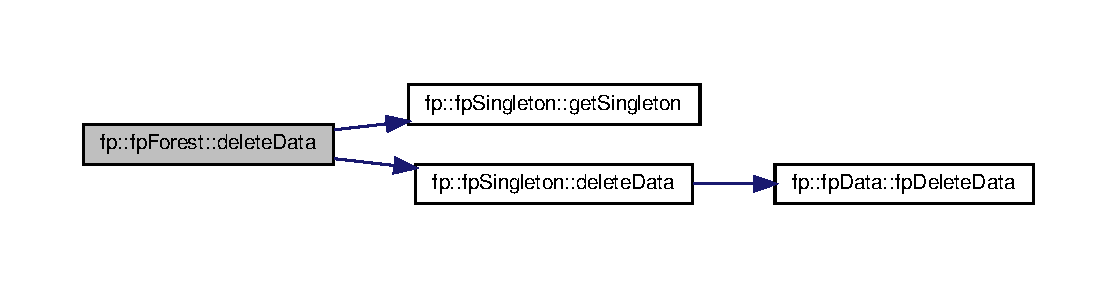
\includegraphics[width=350pt]{classfp_1_1fpForest_a598d32c816dfe5f9793973dcdff2f76e_cgraph}
\end{center}
\end{figure}
\mbox{\Hypertarget{classfp_1_1fpForest_a3eb78e4e61b289853cc45021f2cf3de0}\label{classfp_1_1fpForest_a3eb78e4e61b289853cc45021f2cf3de0}} 
\index{fp\+::fp\+Forest@{fp\+::fp\+Forest}!delete\+Test\+Data@{delete\+Test\+Data}}
\index{delete\+Test\+Data@{delete\+Test\+Data}!fp\+::fp\+Forest@{fp\+::fp\+Forest}}
\subsubsection{\texorpdfstring{delete\+Test\+Data()}{deleteTestData()}}
{\footnotesize\ttfamily void fp\+::fp\+Forest\+::delete\+Test\+Data (\begin{DoxyParamCaption}{ }\end{DoxyParamCaption})\hspace{0.3cm}{\ttfamily [inline]}, {\ttfamily [protected]}}



Definition at line 27 of file fp\+Forest.\+h.


\begin{DoxyCode}
27                                  \{
28                 \hyperlink{classfp_1_1fpSingleton_a8bdae77b68521003e3fc630edec2e240}{fpSingleton::getSingleton}().
      \hyperlink{classfp_1_1fpSingleton_aa4ac02c580b06ba16ed0160ec694438d}{deleteTestData}();
29             \}
\end{DoxyCode}
Here is the call graph for this function\+:\nopagebreak
\begin{figure}[H]
\begin{center}
\leavevmode
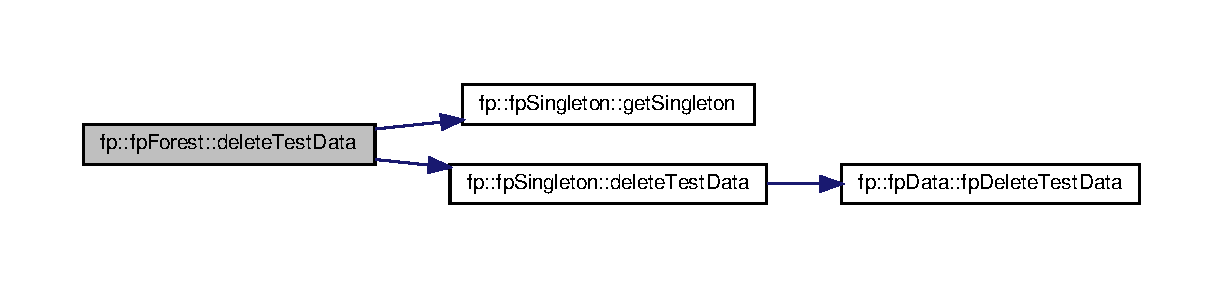
\includegraphics[width=350pt]{classfp_1_1fpForest_a3eb78e4e61b289853cc45021f2cf3de0_cgraph}
\end{center}
\end{figure}
\mbox{\Hypertarget{classfp_1_1fpForest_ac617e33890e96ee5e96e286a45d245fe}\label{classfp_1_1fpForest_ac617e33890e96ee5e96e286a45d245fe}} 
\index{fp\+::fp\+Forest@{fp\+::fp\+Forest}!grow\+Forest@{grow\+Forest}}
\index{grow\+Forest@{grow\+Forest}!fp\+::fp\+Forest@{fp\+::fp\+Forest}}
\subsubsection{\texorpdfstring{grow\+Forest()}{growForest()}}
{\footnotesize\ttfamily void fp\+::fp\+Forest\+::grow\+Forest (\begin{DoxyParamCaption}{ }\end{DoxyParamCaption})\hspace{0.3cm}{\ttfamily [inline]}}



Definition at line 71 of file fp\+Forest.\+h.


\begin{DoxyCode}
71                              \{
72                 \hyperlink{classfp_1_1fpForest_a01631065f4909f10cea4b690084a345a}{loadData}();
73                 \hyperlink{classfp_1_1fpForest_a776ae408ea6c9af459e6ebba7e363d57}{initializeForestType}();
74                 \hyperlink{classfp_1_1fpForest_a846818c46a4423f668f19d3493864192}{setDataDependentParameters}();
75                 \textcolor{comment}{//timeLogger x;}
76                 \textcolor{comment}{//x.startGrowTimer();}
77                 \hyperlink{classfp_1_1fpForest_a4ce6af867d36c8d62c860db8982235c4}{forest}->growForest();
78                 \textcolor{comment}{//x.stopGrowTimer();}
79                 \textcolor{comment}{//x.printGrowTime();}
80                 \hyperlink{classfp_1_1fpForest_a598d32c816dfe5f9793973dcdff2f76e}{deleteData}();
81             \}
\end{DoxyCode}
Here is the call graph for this function\+:
\nopagebreak
\begin{figure}[H]
\begin{center}
\leavevmode
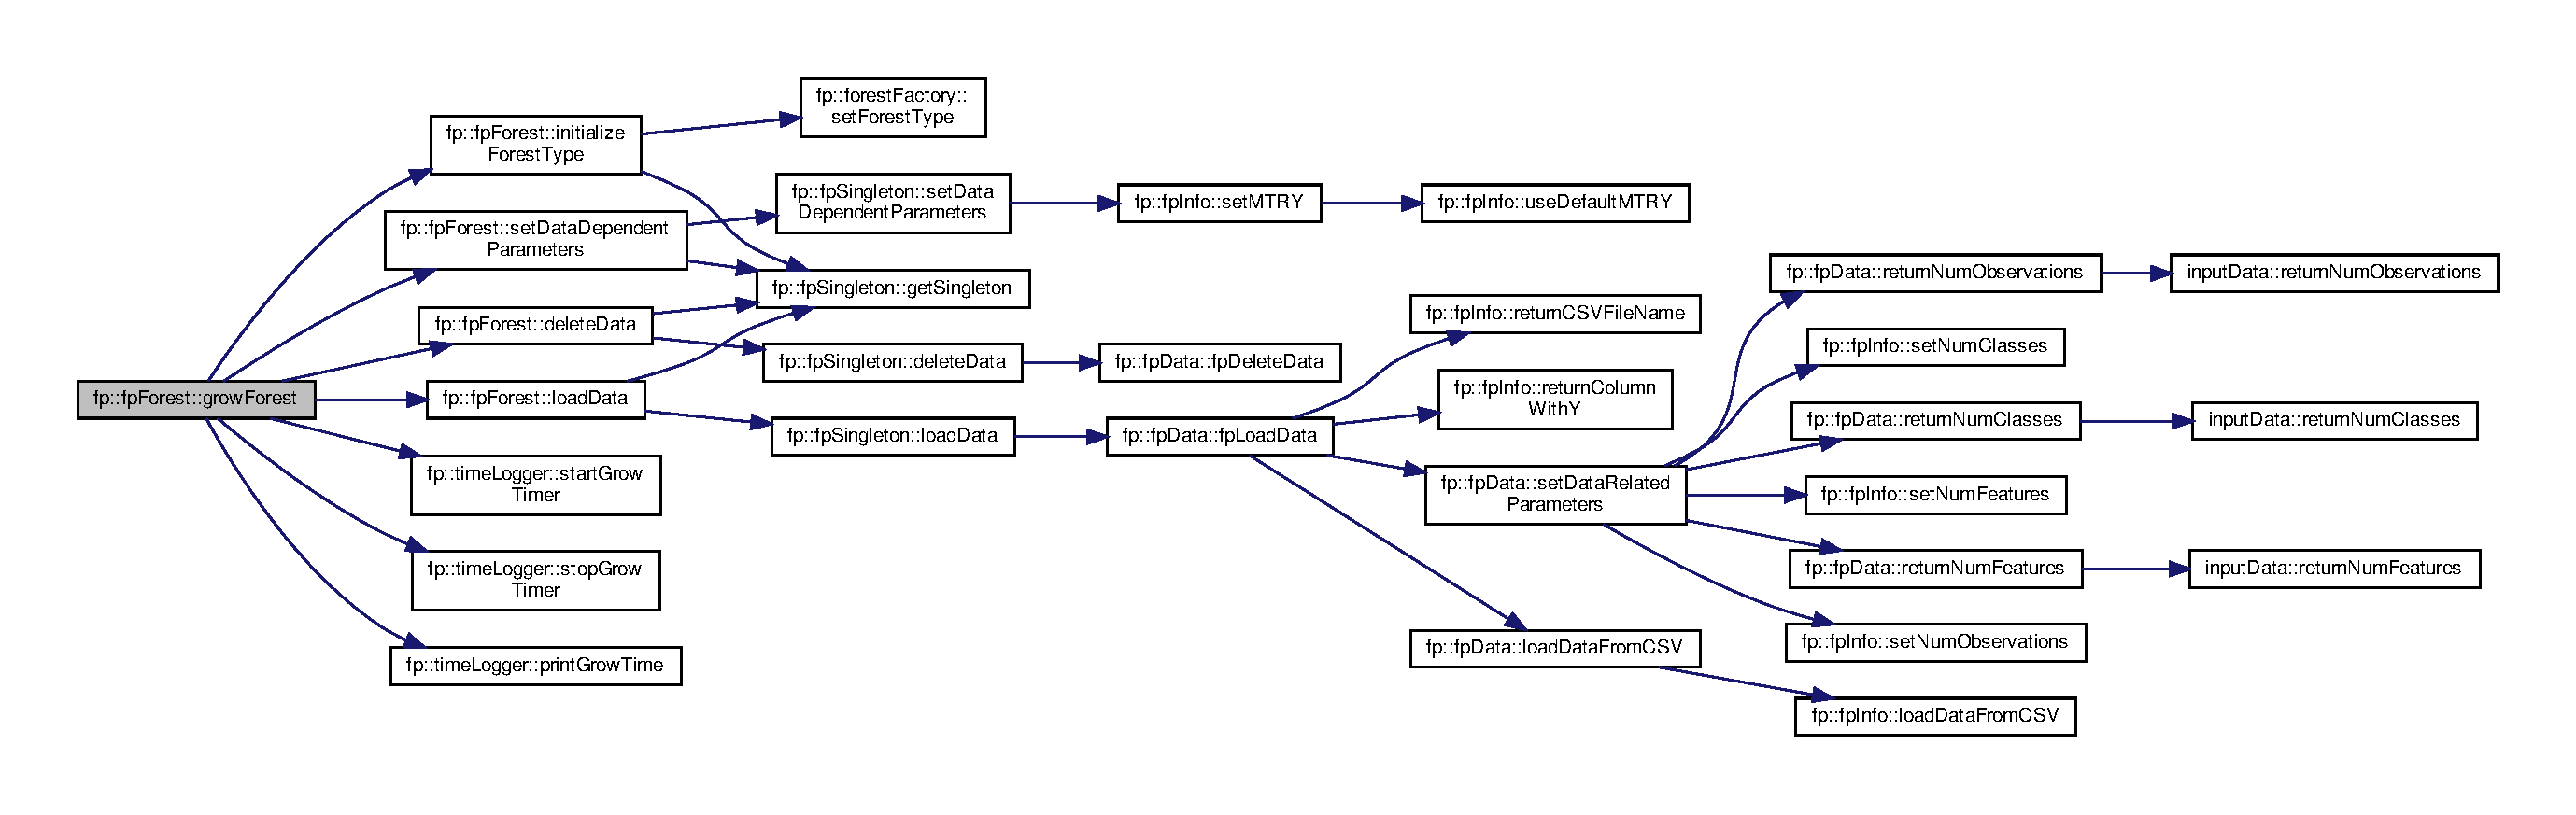
\includegraphics[width=350pt]{classfp_1_1fpForest_ac617e33890e96ee5e96e286a45d245fe_cgraph}
\end{center}
\end{figure}
\mbox{\Hypertarget{classfp_1_1fpForest_a776ae408ea6c9af459e6ebba7e363d57}\label{classfp_1_1fpForest_a776ae408ea6c9af459e6ebba7e363d57}} 
\index{fp\+::fp\+Forest@{fp\+::fp\+Forest}!initialize\+Forest\+Type@{initialize\+Forest\+Type}}
\index{initialize\+Forest\+Type@{initialize\+Forest\+Type}!fp\+::fp\+Forest@{fp\+::fp\+Forest}}
\subsubsection{\texorpdfstring{initialize\+Forest\+Type()}{initializeForestType()}}
{\footnotesize\ttfamily void fp\+::fp\+Forest\+::initialize\+Forest\+Type (\begin{DoxyParamCaption}{ }\end{DoxyParamCaption})\hspace{0.3cm}{\ttfamily [inline]}, {\ttfamily [protected]}}



Definition at line 36 of file fp\+Forest.\+h.


\begin{DoxyCode}
36                                               \{
37                 \hyperlink{classfp_1_1fpForest_a4ce6af867d36c8d62c860db8982235c4}{forest} = \hyperlink{classfp_1_1forestFactory_a856050d77f96dd155d41b95684552c20}{forestFactory::setForestType}(
      \hyperlink{classfp_1_1fpSingleton_a8bdae77b68521003e3fc630edec2e240}{fpSingleton::getSingleton}().returnForestType());
38             \}
\end{DoxyCode}
Here is the call graph for this function\+:
\nopagebreak
\begin{figure}[H]
\begin{center}
\leavevmode
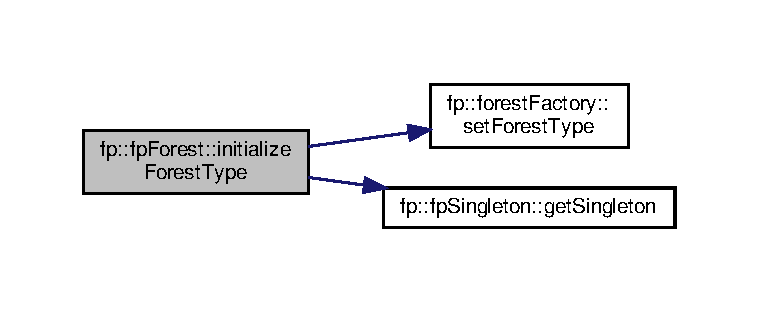
\includegraphics[width=350pt]{classfp_1_1fpForest_a776ae408ea6c9af459e6ebba7e363d57_cgraph}
\end{center}
\end{figure}
\mbox{\Hypertarget{classfp_1_1fpForest_a01631065f4909f10cea4b690084a345a}\label{classfp_1_1fpForest_a01631065f4909f10cea4b690084a345a}} 
\index{fp\+::fp\+Forest@{fp\+::fp\+Forest}!load\+Data@{load\+Data}}
\index{load\+Data@{load\+Data}!fp\+::fp\+Forest@{fp\+::fp\+Forest}}
\subsubsection{\texorpdfstring{load\+Data()}{loadData()}}
{\footnotesize\ttfamily void fp\+::fp\+Forest\+::load\+Data (\begin{DoxyParamCaption}{ }\end{DoxyParamCaption})\hspace{0.3cm}{\ttfamily [inline]}, {\ttfamily [protected]}}



Definition at line 15 of file fp\+Forest.\+h.


\begin{DoxyCode}
15                            \{
16                 \hyperlink{classfp_1_1fpSingleton_a8bdae77b68521003e3fc630edec2e240}{fpSingleton::getSingleton}().\hyperlink{classfp_1_1fpSingleton_a86042ae6be6f59dfb90232678350011a}{loadData}();
17             \}
\end{DoxyCode}
Here is the call graph for this function\+:
\nopagebreak
\begin{figure}[H]
\begin{center}
\leavevmode
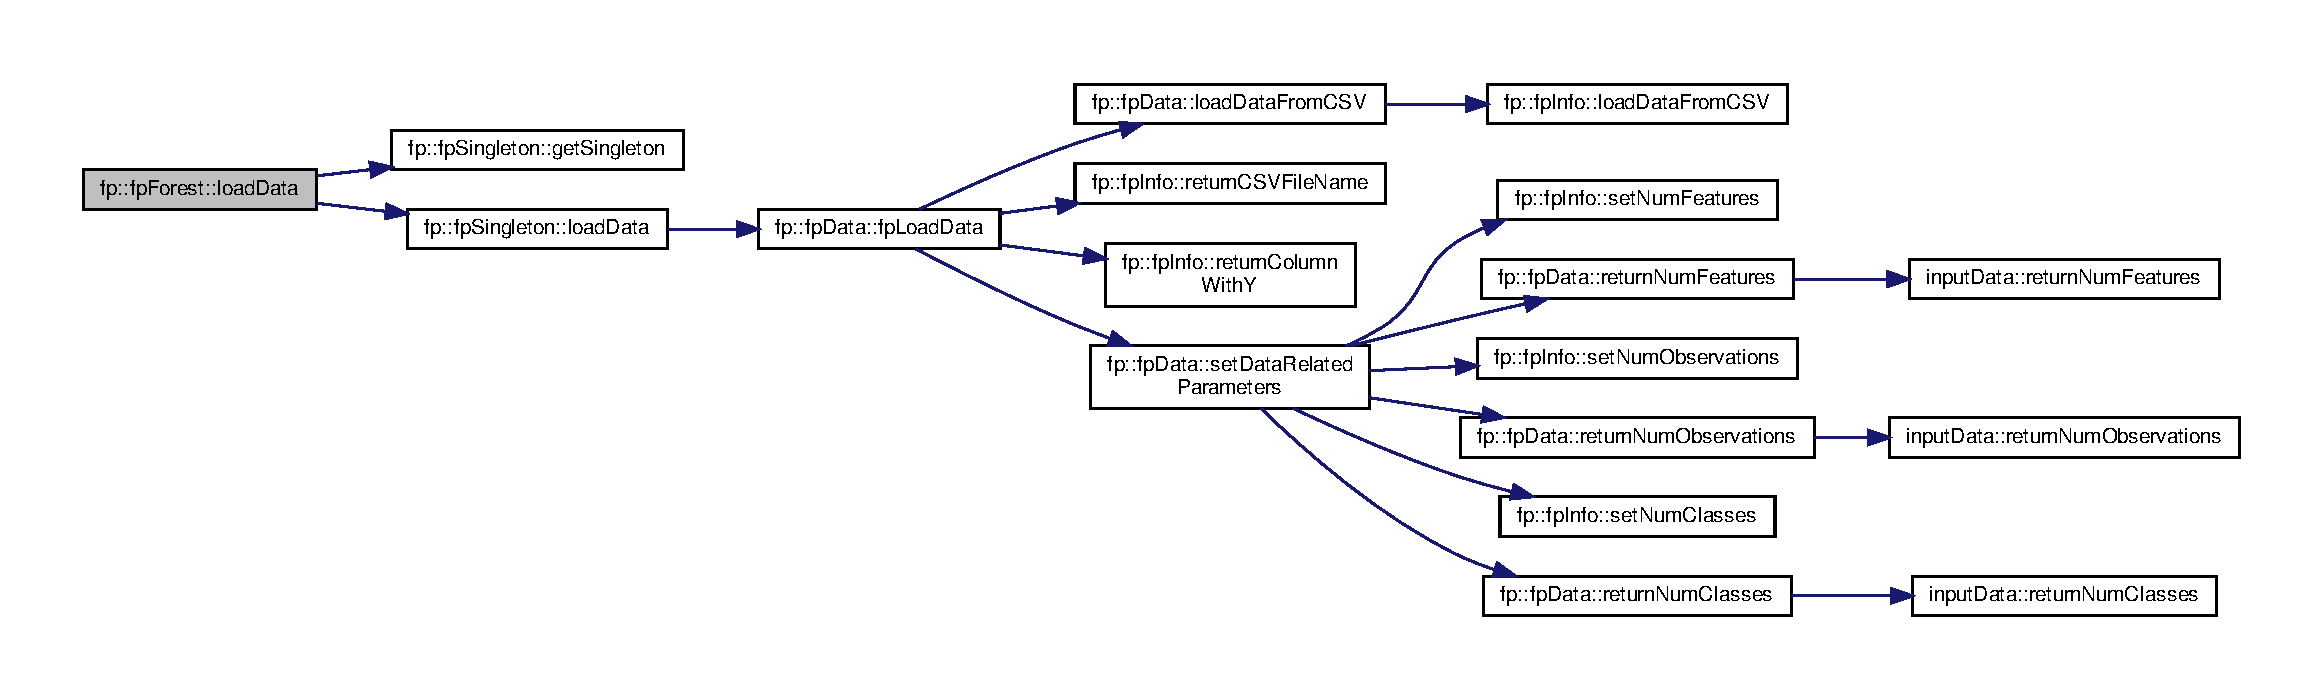
\includegraphics[width=350pt]{classfp_1_1fpForest_a01631065f4909f10cea4b690084a345a_cgraph}
\end{center}
\end{figure}
\mbox{\Hypertarget{classfp_1_1fpForest_abdcf008b65b6af7be5428d838b33be32}\label{classfp_1_1fpForest_abdcf008b65b6af7be5428d838b33be32}} 
\index{fp\+::fp\+Forest@{fp\+::fp\+Forest}!load\+Test\+Data@{load\+Test\+Data}}
\index{load\+Test\+Data@{load\+Test\+Data}!fp\+::fp\+Forest@{fp\+::fp\+Forest}}
\subsubsection{\texorpdfstring{load\+Test\+Data()}{loadTestData()}}
{\footnotesize\ttfamily void fp\+::fp\+Forest\+::load\+Test\+Data (\begin{DoxyParamCaption}{ }\end{DoxyParamCaption})\hspace{0.3cm}{\ttfamily [inline]}, {\ttfamily [protected]}}



Definition at line 19 of file fp\+Forest.\+h.


\begin{DoxyCode}
19                                \{
20                 \hyperlink{classfp_1_1fpSingleton_a8bdae77b68521003e3fc630edec2e240}{fpSingleton::getSingleton}().
      \hyperlink{classfp_1_1fpSingleton_aea7c3b65ded387322d7d5ce48ab96215}{loadTestData}();
21             \}
\end{DoxyCode}
Here is the call graph for this function\+:
\nopagebreak
\begin{figure}[H]
\begin{center}
\leavevmode
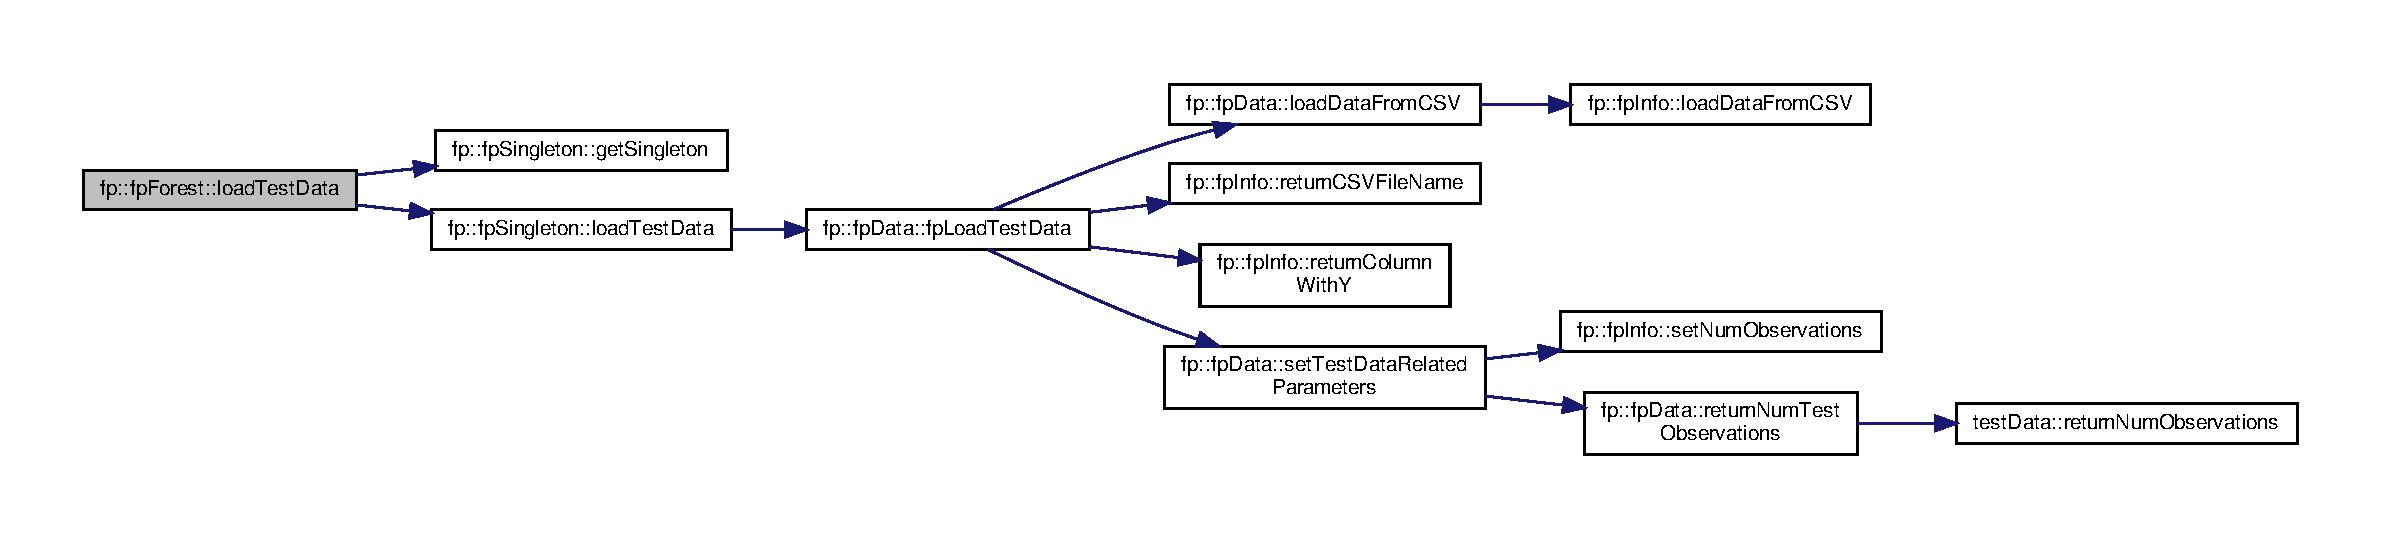
\includegraphics[width=350pt]{classfp_1_1fpForest_abdcf008b65b6af7be5428d838b33be32_cgraph}
\end{center}
\end{figure}
\mbox{\Hypertarget{classfp_1_1fpForest_a4a7ffa92224570d6a97eff8bd5e9b0fa}\label{classfp_1_1fpForest_a4a7ffa92224570d6a97eff8bd5e9b0fa}} 
\index{fp\+::fp\+Forest@{fp\+::fp\+Forest}!print\+Forest\+Type@{print\+Forest\+Type}}
\index{print\+Forest\+Type@{print\+Forest\+Type}!fp\+::fp\+Forest@{fp\+::fp\+Forest}}
\subsubsection{\texorpdfstring{print\+Forest\+Type()}{printForestType()}}
{\footnotesize\ttfamily void fp\+::fp\+Forest\+::print\+Forest\+Type (\begin{DoxyParamCaption}{ }\end{DoxyParamCaption})\hspace{0.3cm}{\ttfamily [inline]}}



Definition at line 66 of file fp\+Forest.\+h.


\begin{DoxyCode}
66                                          \{
67                 \hyperlink{classfp_1_1fpSingleton_a8bdae77b68521003e3fc630edec2e240}{fpSingleton::getSingleton}().
      \hyperlink{classfp_1_1fpSingleton_ad9696336521f72c7c6a021608799871e}{printForestType}();
68             \}
\end{DoxyCode}
Here is the call graph for this function\+:
\nopagebreak
\begin{figure}[H]
\begin{center}
\leavevmode
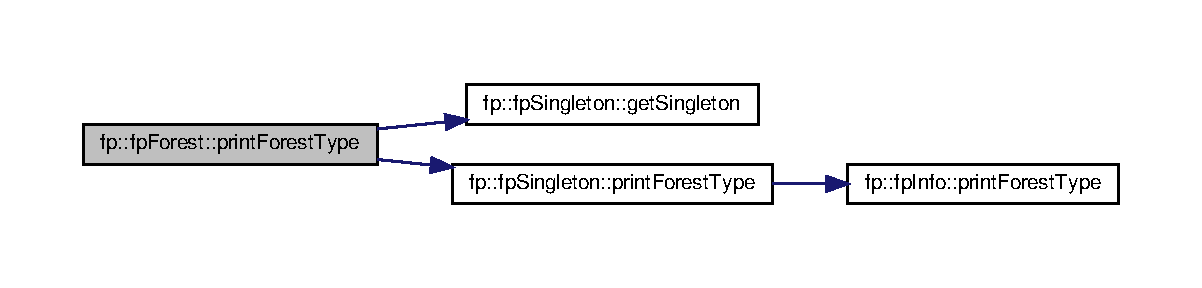
\includegraphics[width=350pt]{classfp_1_1fpForest_a4a7ffa92224570d6a97eff8bd5e9b0fa_cgraph}
\end{center}
\end{figure}
\mbox{\Hypertarget{classfp_1_1fpForest_ae096def0ca26f0771b27341d7b218066}\label{classfp_1_1fpForest_ae096def0ca26f0771b27341d7b218066}} 
\index{fp\+::fp\+Forest@{fp\+::fp\+Forest}!print\+Parameters@{print\+Parameters}}
\index{print\+Parameters@{print\+Parameters}!fp\+::fp\+Forest@{fp\+::fp\+Forest}}
\subsubsection{\texorpdfstring{print\+Parameters()}{printParameters()}}
{\footnotesize\ttfamily void fp\+::fp\+Forest\+::print\+Parameters (\begin{DoxyParamCaption}{ }\end{DoxyParamCaption})\hspace{0.3cm}{\ttfamily [inline]}}



Definition at line 62 of file fp\+Forest.\+h.


\begin{DoxyCode}
62                                          \{
63                 \hyperlink{classfp_1_1fpSingleton_a8bdae77b68521003e3fc630edec2e240}{fpSingleton::getSingleton}().
      \hyperlink{classfp_1_1fpSingleton_a0d769b6652e4c74c2734cdc811eeab5a}{printAllParameters}();
64             \}
\end{DoxyCode}
Here is the call graph for this function\+:
\nopagebreak
\begin{figure}[H]
\begin{center}
\leavevmode
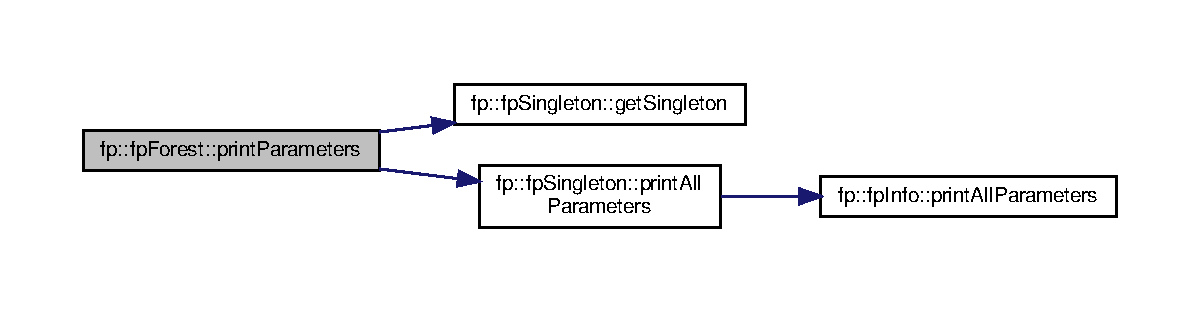
\includegraphics[width=350pt]{classfp_1_1fpForest_ae096def0ca26f0771b27341d7b218066_cgraph}
\end{center}
\end{figure}
\mbox{\Hypertarget{classfp_1_1fpForest_a846818c46a4423f668f19d3493864192}\label{classfp_1_1fpForest_a846818c46a4423f668f19d3493864192}} 
\index{fp\+::fp\+Forest@{fp\+::fp\+Forest}!set\+Data\+Dependent\+Parameters@{set\+Data\+Dependent\+Parameters}}
\index{set\+Data\+Dependent\+Parameters@{set\+Data\+Dependent\+Parameters}!fp\+::fp\+Forest@{fp\+::fp\+Forest}}
\subsubsection{\texorpdfstring{set\+Data\+Dependent\+Parameters()}{setDataDependentParameters()}}
{\footnotesize\ttfamily void fp\+::fp\+Forest\+::set\+Data\+Dependent\+Parameters (\begin{DoxyParamCaption}{ }\end{DoxyParamCaption})\hspace{0.3cm}{\ttfamily [inline]}, {\ttfamily [protected]}}



Definition at line 40 of file fp\+Forest.\+h.


\begin{DoxyCode}
40                                                     \{
41                 \hyperlink{classfp_1_1fpSingleton_a8bdae77b68521003e3fc630edec2e240}{fpSingleton::getSingleton}().
      \hyperlink{classfp_1_1fpSingleton_a3edf17209500e72c76ef816e32666eb2}{setDataDependentParameters}();
42             \}
\end{DoxyCode}
Here is the call graph for this function\+:
\nopagebreak
\begin{figure}[H]
\begin{center}
\leavevmode
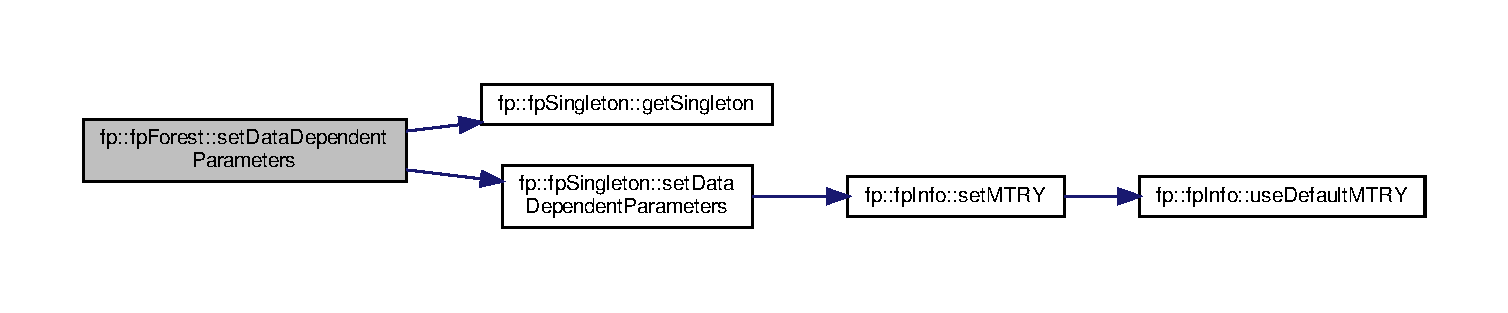
\includegraphics[width=350pt]{classfp_1_1fpForest_a846818c46a4423f668f19d3493864192_cgraph}
\end{center}
\end{figure}
\mbox{\Hypertarget{classfp_1_1fpForest_ab25fdbad494f8bd358ccb3a1fdbcb51d}\label{classfp_1_1fpForest_ab25fdbad494f8bd358ccb3a1fdbcb51d}} 
\index{fp\+::fp\+Forest@{fp\+::fp\+Forest}!set\+Function\+Pointers@{set\+Function\+Pointers}}
\index{set\+Function\+Pointers@{set\+Function\+Pointers}!fp\+::fp\+Forest@{fp\+::fp\+Forest}}
\subsubsection{\texorpdfstring{set\+Function\+Pointers()}{setFunctionPointers()}}
{\footnotesize\ttfamily void fp\+::fp\+Forest\+::set\+Function\+Pointers (\begin{DoxyParamCaption}{ }\end{DoxyParamCaption})\hspace{0.3cm}{\ttfamily [inline]}, {\ttfamily [protected]}}



Definition at line 32 of file fp\+Forest.\+h.


\begin{DoxyCode}
32                                              \{
33                 ;\textcolor{comment}{//fpSingleton::getSingleton().setFunctionPointers();}
34             \}
\end{DoxyCode}
\mbox{\Hypertarget{classfp_1_1fpForest_ad13bbbd33291ef5f523691eccc23aece}\label{classfp_1_1fpForest_ad13bbbd33291ef5f523691eccc23aece}} 
\index{fp\+::fp\+Forest@{fp\+::fp\+Forest}!set\+Parameter@{set\+Parameter}}
\index{set\+Parameter@{set\+Parameter}!fp\+::fp\+Forest@{fp\+::fp\+Forest}}
\subsubsection{\texorpdfstring{set\+Parameter()}{setParameter()}\hspace{0.1cm}{\footnotesize\ttfamily [1/3]}}
{\footnotesize\ttfamily void fp\+::fp\+Forest\+::set\+Parameter (\begin{DoxyParamCaption}\item[{const std\+::string \&}]{parameter\+Name,  }\item[{const std\+::string \&}]{parameter\+Value }\end{DoxyParamCaption})\hspace{0.3cm}{\ttfamily [inline]}}



Definition at line 49 of file fp\+Forest.\+h.


\begin{DoxyCode}
49                                                                                                      \{
50                 \hyperlink{classfp_1_1fpSingleton_a8bdae77b68521003e3fc630edec2e240}{fpSingleton::getSingleton}().
      \hyperlink{classfp_1_1fpSingleton_a90f275b256694ea7b16577d547a33044}{setParameter}(parameterName, parameterValue);    
51             \}
\end{DoxyCode}
Here is the call graph for this function\+:
\nopagebreak
\begin{figure}[H]
\begin{center}
\leavevmode
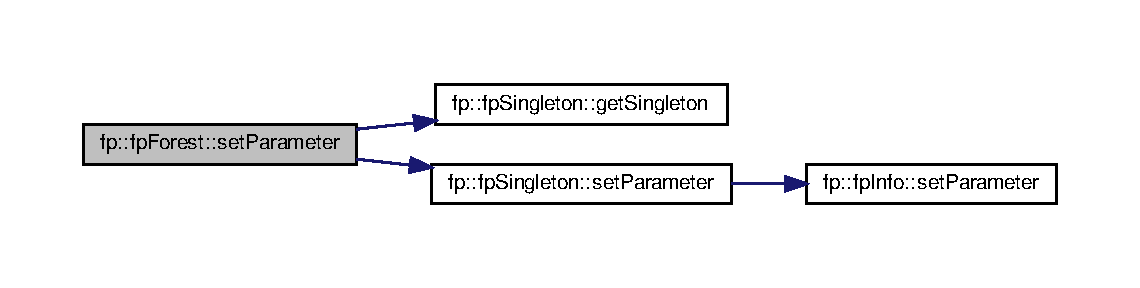
\includegraphics[width=350pt]{classfp_1_1fpForest_ad13bbbd33291ef5f523691eccc23aece_cgraph}
\end{center}
\end{figure}
\mbox{\Hypertarget{classfp_1_1fpForest_afc7a14e083aaae0dbd90ef0a30c48c21}\label{classfp_1_1fpForest_afc7a14e083aaae0dbd90ef0a30c48c21}} 
\index{fp\+::fp\+Forest@{fp\+::fp\+Forest}!set\+Parameter@{set\+Parameter}}
\index{set\+Parameter@{set\+Parameter}!fp\+::fp\+Forest@{fp\+::fp\+Forest}}
\subsubsection{\texorpdfstring{set\+Parameter()}{setParameter()}\hspace{0.1cm}{\footnotesize\ttfamily [2/3]}}
{\footnotesize\ttfamily void fp\+::fp\+Forest\+::set\+Parameter (\begin{DoxyParamCaption}\item[{const std\+::string \&}]{parameter\+Name,  }\item[{const double}]{parameter\+Value }\end{DoxyParamCaption})\hspace{0.3cm}{\ttfamily [inline]}}



Definition at line 54 of file fp\+Forest.\+h.


\begin{DoxyCode}
54                                                                                                  \{
55                 \hyperlink{classfp_1_1fpSingleton_a8bdae77b68521003e3fc630edec2e240}{fpSingleton::getSingleton}().
      \hyperlink{classfp_1_1fpSingleton_a90f275b256694ea7b16577d547a33044}{setParameter}(parameterName, parameterValue);    
56             \}
\end{DoxyCode}
Here is the call graph for this function\+:
\nopagebreak
\begin{figure}[H]
\begin{center}
\leavevmode
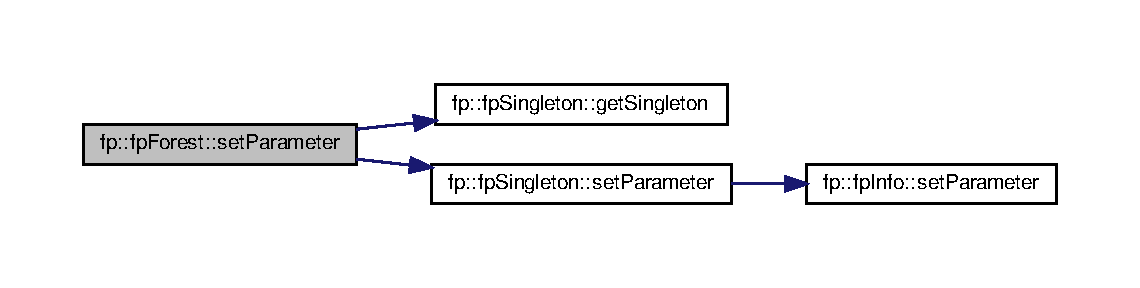
\includegraphics[width=350pt]{classfp_1_1fpForest_afc7a14e083aaae0dbd90ef0a30c48c21_cgraph}
\end{center}
\end{figure}
\mbox{\Hypertarget{classfp_1_1fpForest_a8a083cc4cd4110dee2b6627d53529965}\label{classfp_1_1fpForest_a8a083cc4cd4110dee2b6627d53529965}} 
\index{fp\+::fp\+Forest@{fp\+::fp\+Forest}!set\+Parameter@{set\+Parameter}}
\index{set\+Parameter@{set\+Parameter}!fp\+::fp\+Forest@{fp\+::fp\+Forest}}
\subsubsection{\texorpdfstring{set\+Parameter()}{setParameter()}\hspace{0.1cm}{\footnotesize\ttfamily [3/3]}}
{\footnotesize\ttfamily void fp\+::fp\+Forest\+::set\+Parameter (\begin{DoxyParamCaption}\item[{const std\+::string \&}]{parameter\+Name,  }\item[{const int}]{parameter\+Value }\end{DoxyParamCaption})\hspace{0.3cm}{\ttfamily [inline]}}



Definition at line 58 of file fp\+Forest.\+h.


\begin{DoxyCode}
58                                                                                               \{
59                 \hyperlink{classfp_1_1fpSingleton_a8bdae77b68521003e3fc630edec2e240}{fpSingleton::getSingleton}().
      \hyperlink{classfp_1_1fpSingleton_a90f275b256694ea7b16577d547a33044}{setParameter}(parameterName, parameterValue);    
60             \}
\end{DoxyCode}
Here is the call graph for this function\+:
\nopagebreak
\begin{figure}[H]
\begin{center}
\leavevmode
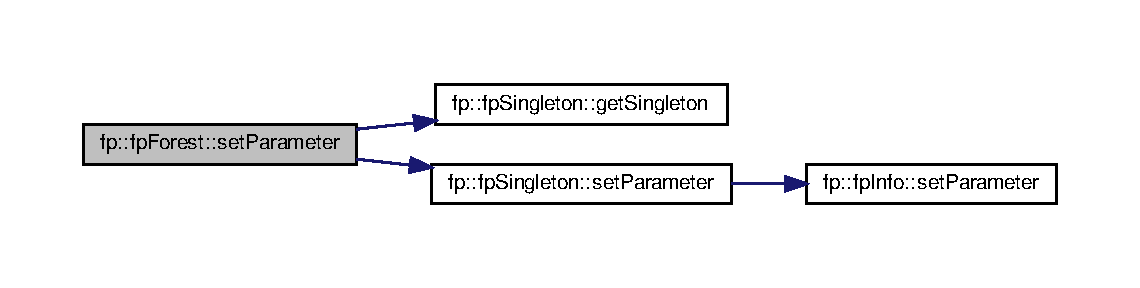
\includegraphics[width=350pt]{classfp_1_1fpForest_a8a083cc4cd4110dee2b6627d53529965_cgraph}
\end{center}
\end{figure}
\mbox{\Hypertarget{classfp_1_1fpForest_a2ecaa11b48f37781f5fb4607ed6a490f}\label{classfp_1_1fpForest_a2ecaa11b48f37781f5fb4607ed6a490f}} 
\index{fp\+::fp\+Forest@{fp\+::fp\+Forest}!test\+Accuracy@{test\+Accuracy}}
\index{test\+Accuracy@{test\+Accuracy}!fp\+::fp\+Forest@{fp\+::fp\+Forest}}
\subsubsection{\texorpdfstring{test\+Accuracy()}{testAccuracy()}}
{\footnotesize\ttfamily float fp\+::fp\+Forest\+::test\+Accuracy (\begin{DoxyParamCaption}{ }\end{DoxyParamCaption})\hspace{0.3cm}{\ttfamily [inline]}}



Definition at line 84 of file fp\+Forest.\+h.


\begin{DoxyCode}
84                                 \{
85                 \textcolor{keywordtype}{float} testError;
86                 \hyperlink{classfp_1_1fpForest_abdcf008b65b6af7be5428d838b33be32}{loadTestData}();
87                 testError = \hyperlink{classfp_1_1fpForest_a4ce6af867d36c8d62c860db8982235c4}{forest}->testForest();
88                 \hyperlink{classfp_1_1fpForest_a3eb78e4e61b289853cc45021f2cf3de0}{deleteTestData}();
89                 \textcolor{keywordflow}{return} testError;
90             \}
\end{DoxyCode}
Here is the call graph for this function\+:
\nopagebreak
\begin{figure}[H]
\begin{center}
\leavevmode
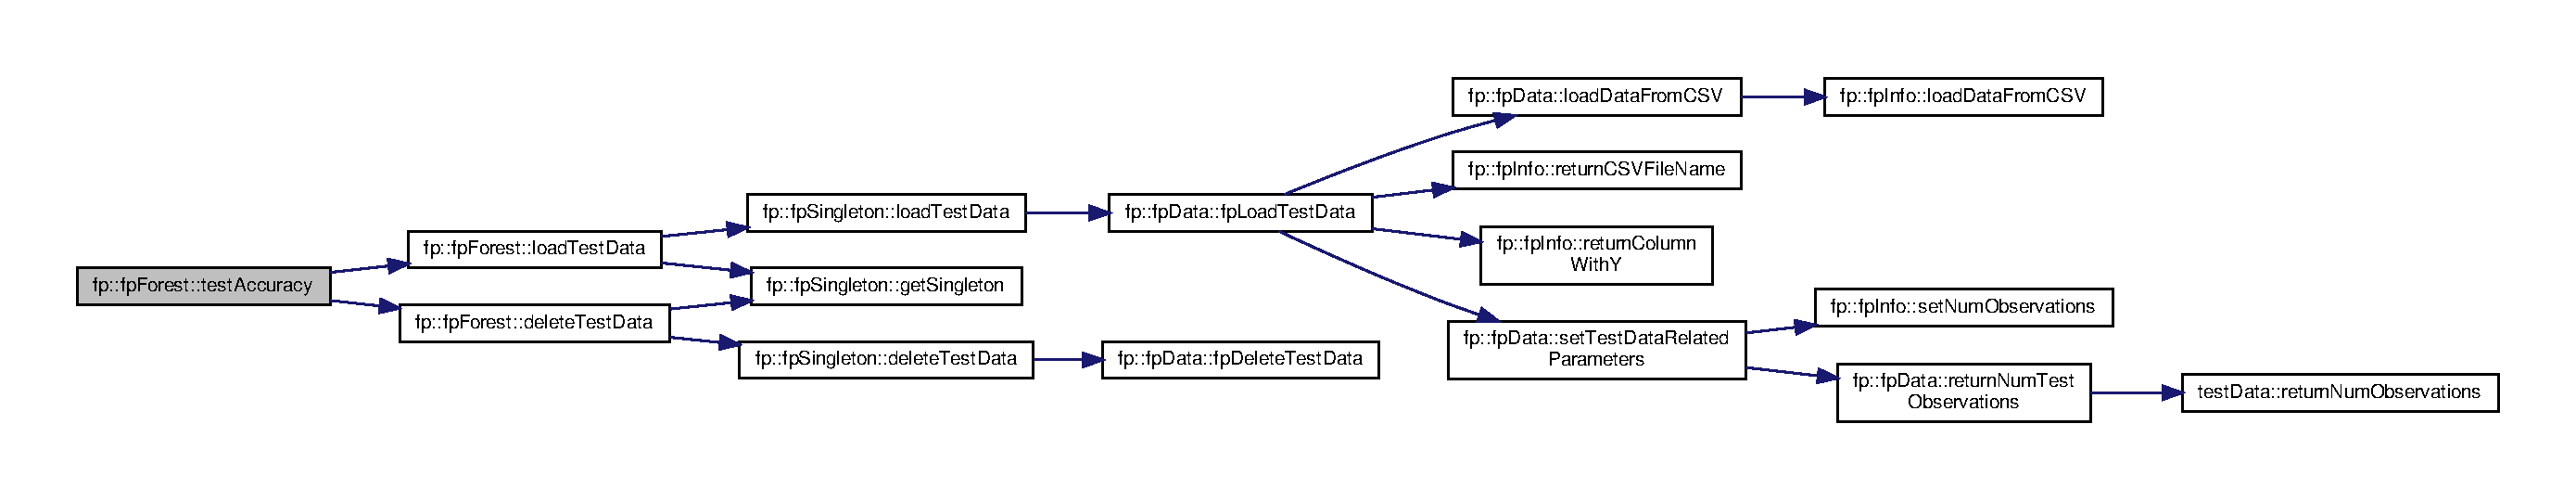
\includegraphics[width=350pt]{classfp_1_1fpForest_a2ecaa11b48f37781f5fb4607ed6a490f_cgraph}
\end{center}
\end{figure}


\subsection{Member Data Documentation}
\mbox{\Hypertarget{classfp_1_1fpForest_a4ce6af867d36c8d62c860db8982235c4}\label{classfp_1_1fpForest_a4ce6af867d36c8d62c860db8982235c4}} 
\index{fp\+::fp\+Forest@{fp\+::fp\+Forest}!forest@{forest}}
\index{forest@{forest}!fp\+::fp\+Forest@{fp\+::fp\+Forest}}
\subsubsection{\texorpdfstring{forest}{forest}}
{\footnotesize\ttfamily std\+::unique\+\_\+ptr$<$\hyperlink{classfp_1_1fpForestBase}{fp\+Forest\+Base}$>$ fp\+::fp\+Forest\+::forest\hspace{0.3cm}{\ttfamily [protected]}}



Definition at line 13 of file fp\+Forest.\+h.



The documentation for this class was generated from the following file\+:\begin{DoxyCompactItemize}
\item 
src/base\+Functions/\hyperlink{fpForest_8h}{fp\+Forest.\+h}\end{DoxyCompactItemize}

\hypertarget{classfp_1_1fpForestBase}{}\section{fp\+:\+:fp\+Forest\+Base Class Reference}
\label{classfp_1_1fpForestBase}\index{fp\+::fp\+Forest\+Base@{fp\+::fp\+Forest\+Base}}


{\ttfamily \#include $<$fp\+Forest\+Base.\+h$>$}



Inheritance diagram for fp\+:\+:fp\+Forest\+Base\+:\nopagebreak
\begin{figure}[H]
\begin{center}
\leavevmode
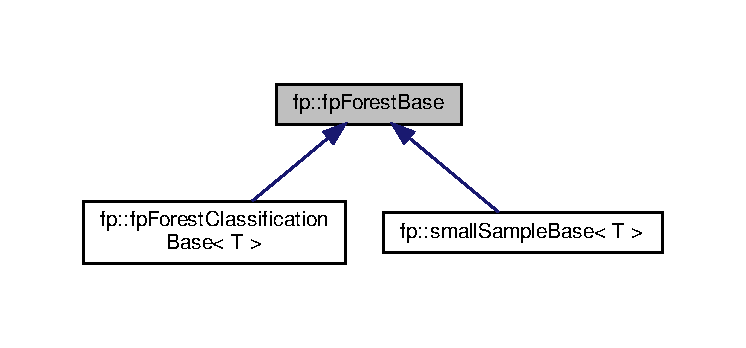
\includegraphics[width=350pt]{classfp_1_1fpForestBase__inherit__graph}
\end{center}
\end{figure}
\subsection*{Public Member Functions}
\begin{DoxyCompactItemize}
\item 
virtual void \hyperlink{classfp_1_1fpForestBase_a5e200f603cca94bb5d9f357489f07e97}{print\+Forest\+Type} ()=0
\item 
virtual void \hyperlink{classfp_1_1fpForestBase_a05b1d924a559536083ee7a8cf3ea542d}{grow\+Forest} ()=0
\item 
virtual float \hyperlink{classfp_1_1fpForestBase_af7becba028a198f650841b718d16ed16}{test\+Forest} ()=0
\end{DoxyCompactItemize}


\subsection{Detailed Description}


Definition at line 7 of file fp\+Forest\+Base.\+h.



\subsection{Member Function Documentation}
\mbox{\Hypertarget{classfp_1_1fpForestBase_a05b1d924a559536083ee7a8cf3ea542d}\label{classfp_1_1fpForestBase_a05b1d924a559536083ee7a8cf3ea542d}} 
\index{fp\+::fp\+Forest\+Base@{fp\+::fp\+Forest\+Base}!grow\+Forest@{grow\+Forest}}
\index{grow\+Forest@{grow\+Forest}!fp\+::fp\+Forest\+Base@{fp\+::fp\+Forest\+Base}}
\subsubsection{\texorpdfstring{grow\+Forest()}{growForest()}}
{\footnotesize\ttfamily virtual void fp\+::fp\+Forest\+Base\+::grow\+Forest (\begin{DoxyParamCaption}{ }\end{DoxyParamCaption})\hspace{0.3cm}{\ttfamily [pure virtual]}}



Implemented in \hyperlink{classfp_1_1fpForestClassificationBase_a706225fdbef8c71fb022f4c3446b388d}{fp\+::fp\+Forest\+Classification\+Base$<$ T $>$}, and \hyperlink{classfp_1_1smallSampleBase_a8c5b6a0f2c8aeb32a322cc5e237c60af}{fp\+::small\+Sample\+Base$<$ T $>$}.

\mbox{\Hypertarget{classfp_1_1fpForestBase_a5e200f603cca94bb5d9f357489f07e97}\label{classfp_1_1fpForestBase_a5e200f603cca94bb5d9f357489f07e97}} 
\index{fp\+::fp\+Forest\+Base@{fp\+::fp\+Forest\+Base}!print\+Forest\+Type@{print\+Forest\+Type}}
\index{print\+Forest\+Type@{print\+Forest\+Type}!fp\+::fp\+Forest\+Base@{fp\+::fp\+Forest\+Base}}
\subsubsection{\texorpdfstring{print\+Forest\+Type()}{printForestType()}}
{\footnotesize\ttfamily virtual void fp\+::fp\+Forest\+Base\+::print\+Forest\+Type (\begin{DoxyParamCaption}{ }\end{DoxyParamCaption})\hspace{0.3cm}{\ttfamily [pure virtual]}}



Implemented in \hyperlink{classfp_1_1fpForestClassificationBase_a6b5243d32b468308a4f013ad5a9df2dd}{fp\+::fp\+Forest\+Classification\+Base$<$ T $>$}, and \hyperlink{classfp_1_1smallSampleBase_a1e3244a9a15d53d38e6c9ca78d8d062e}{fp\+::small\+Sample\+Base$<$ T $>$}.

\mbox{\Hypertarget{classfp_1_1fpForestBase_af7becba028a198f650841b718d16ed16}\label{classfp_1_1fpForestBase_af7becba028a198f650841b718d16ed16}} 
\index{fp\+::fp\+Forest\+Base@{fp\+::fp\+Forest\+Base}!test\+Forest@{test\+Forest}}
\index{test\+Forest@{test\+Forest}!fp\+::fp\+Forest\+Base@{fp\+::fp\+Forest\+Base}}
\subsubsection{\texorpdfstring{test\+Forest()}{testForest()}}
{\footnotesize\ttfamily virtual float fp\+::fp\+Forest\+Base\+::test\+Forest (\begin{DoxyParamCaption}{ }\end{DoxyParamCaption})\hspace{0.3cm}{\ttfamily [pure virtual]}}



Implemented in \hyperlink{classfp_1_1fpForestClassificationBase_a3f1ad5a5cfb3633713d0a81bd1c356e8}{fp\+::fp\+Forest\+Classification\+Base$<$ T $>$}, and \hyperlink{classfp_1_1smallSampleBase_a02b01949b6ed9cc6644b045a468609cc}{fp\+::small\+Sample\+Base$<$ T $>$}.



The documentation for this class was generated from the following file\+:\begin{DoxyCompactItemize}
\item 
src/base\+Functions/\hyperlink{fpForestBase_8h}{fp\+Forest\+Base.\+h}\end{DoxyCompactItemize}

\hypertarget{classfp_1_1fpForestClassificationBase}{}\section{fp\+:\+:fp\+Forest\+Classification\+Base$<$ T $>$ Class Template Reference}
\label{classfp_1_1fpForestClassificationBase}\index{fp\+::fp\+Forest\+Classification\+Base$<$ T $>$@{fp\+::fp\+Forest\+Classification\+Base$<$ T $>$}}


{\ttfamily \#include $<$fp\+Forest\+Classification\+Base.\+h$>$}



Inheritance diagram for fp\+:\+:fp\+Forest\+Classification\+Base$<$ T $>$\+:\nopagebreak
\begin{figure}[H]
\begin{center}
\leavevmode
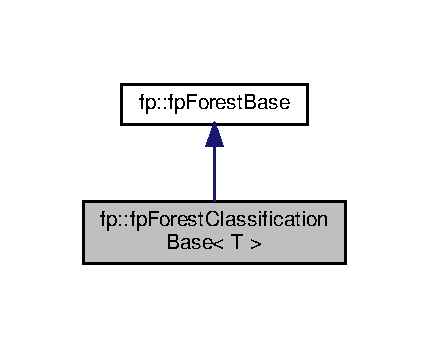
\includegraphics[width=206pt]{classfp_1_1fpForestClassificationBase__inherit__graph}
\end{center}
\end{figure}


Collaboration diagram for fp\+:\+:fp\+Forest\+Classification\+Base$<$ T $>$\+:
\nopagebreak
\begin{figure}[H]
\begin{center}
\leavevmode
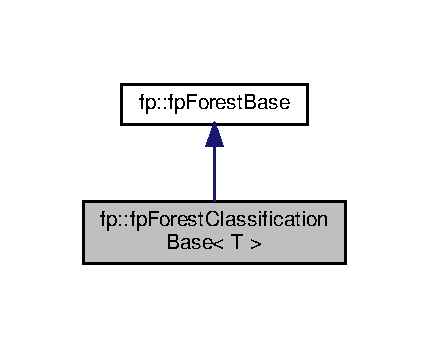
\includegraphics[width=298pt]{classfp_1_1fpForestClassificationBase__coll__graph}
\end{center}
\end{figure}
\subsection*{Public Member Functions}
\begin{DoxyCompactItemize}
\item 
\hyperlink{classfp_1_1fpForestClassificationBase_a788f11473d1b7c86928d021617a92f2a}{fp\+Forest\+Classification\+Base} ()
\item 
void \hyperlink{classfp_1_1fpForestClassificationBase_a6b5243d32b468308a4f013ad5a9df2dd}{print\+Forest\+Type} ()
\item 
void \hyperlink{classfp_1_1fpForestClassificationBase_a696b361df0a1c9aa36687333e2d8111b}{change\+Forest\+Size} ()
\item 
void \hyperlink{classfp_1_1fpForestClassificationBase_aea9db2571269f0f627226aa75ec4a694}{grow\+Trees} ()
\item 
void \hyperlink{classfp_1_1fpForestClassificationBase_a3186e3b6471f82df3f69172f67aa7d19}{check\+Parameters} ()
\item 
void \hyperlink{classfp_1_1fpForestClassificationBase_a48567d379434daeccb1540c84674d286}{tree\+Stats} ()
\item 
void \hyperlink{classfp_1_1fpForestClassificationBase_a1989f90fbd27ac90232b7a1071c96a00}{print\+Tree0} ()
\item 
void \hyperlink{classfp_1_1fpForestClassificationBase_a706225fdbef8c71fb022f4c3446b388d}{grow\+Forest} ()
\item 
int \hyperlink{classfp_1_1fpForestClassificationBase_ad0c690fff971fab681467fbcd8762b5f}{predict\+Class} (int observation\+Number)
\item 
float \hyperlink{classfp_1_1fpForestClassificationBase_a3f1ad5a5cfb3633713d0a81bd1c356e8}{test\+Forest} ()
\end{DoxyCompactItemize}
\subsection*{Public Attributes}
\begin{DoxyCompactItemize}
\item 
\hyperlink{classfp_1_1fpDisplayProgress}{fp\+Display\+Progress} \hyperlink{classfp_1_1fpForestClassificationBase_a21148775a113092d6929e0d28e351a2c}{print\+Progress}
\end{DoxyCompactItemize}
\subsection*{Protected Attributes}
\begin{DoxyCompactItemize}
\item 
std\+::vector$<$ \hyperlink{classfp_1_1rfTree}{rf\+Tree}$<$ T $>$ $>$ \hyperlink{classfp_1_1fpForestClassificationBase_a51482a6c95c4b3cb42627f029c2d4662}{trees}
\end{DoxyCompactItemize}


\subsection{Detailed Description}
\subsubsection*{template$<$typename T$>$\newline
class fp\+::fp\+Forest\+Classification\+Base$<$ T $>$}



Definition at line 16 of file fp\+Forest\+Classification\+Base.\+h.



\subsection{Constructor \& Destructor Documentation}
\mbox{\Hypertarget{classfp_1_1fpForestClassificationBase_a788f11473d1b7c86928d021617a92f2a}\label{classfp_1_1fpForestClassificationBase_a788f11473d1b7c86928d021617a92f2a}} 
\index{fp\+::fp\+Forest\+Classification\+Base@{fp\+::fp\+Forest\+Classification\+Base}!fp\+Forest\+Classification\+Base@{fp\+Forest\+Classification\+Base}}
\index{fp\+Forest\+Classification\+Base@{fp\+Forest\+Classification\+Base}!fp\+::fp\+Forest\+Classification\+Base@{fp\+::fp\+Forest\+Classification\+Base}}
\subsubsection{\texorpdfstring{fp\+Forest\+Classification\+Base()}{fpForestClassificationBase()}}
{\footnotesize\ttfamily template$<$typename T $>$ \\
\hyperlink{classfp_1_1fpForestClassificationBase}{fp\+::fp\+Forest\+Classification\+Base}$<$ T $>$\+::\hyperlink{classfp_1_1fpForestClassificationBase}{fp\+Forest\+Classification\+Base} (\begin{DoxyParamCaption}{ }\end{DoxyParamCaption})\hspace{0.3cm}{\ttfamily [inline]}}



Definition at line 24 of file fp\+Forest\+Classification\+Base.\+h.


\begin{DoxyCode}
24                                         \{
25                 std::srand(\textcolor{keywordtype}{unsigned}(std::time(0)));
26             \}
\end{DoxyCode}


\subsection{Member Function Documentation}
\mbox{\Hypertarget{classfp_1_1fpForestClassificationBase_a696b361df0a1c9aa36687333e2d8111b}\label{classfp_1_1fpForestClassificationBase_a696b361df0a1c9aa36687333e2d8111b}} 
\index{fp\+::fp\+Forest\+Classification\+Base@{fp\+::fp\+Forest\+Classification\+Base}!change\+Forest\+Size@{change\+Forest\+Size}}
\index{change\+Forest\+Size@{change\+Forest\+Size}!fp\+::fp\+Forest\+Classification\+Base@{fp\+::fp\+Forest\+Classification\+Base}}
\subsubsection{\texorpdfstring{change\+Forest\+Size()}{changeForestSize()}}
{\footnotesize\ttfamily template$<$typename T $>$ \\
void \hyperlink{classfp_1_1fpForestClassificationBase}{fp\+::fp\+Forest\+Classification\+Base}$<$ T $>$\+::change\+Forest\+Size (\begin{DoxyParamCaption}{ }\end{DoxyParamCaption})\hspace{0.3cm}{\ttfamily [inline]}}



Definition at line 32 of file fp\+Forest\+Classification\+Base.\+h.


\begin{DoxyCode}
32                                    \{
33                 \hyperlink{classfp_1_1fpForestClassificationBase_a51482a6c95c4b3cb42627f029c2d4662}{trees}.resize(\hyperlink{classfp_1_1fpSingleton_a8bdae77b68521003e3fc630edec2e240}{fpSingleton::getSingleton}().returnNumTrees());
34             \}
\end{DoxyCode}
Here is the call graph for this function\+:\nopagebreak
\begin{figure}[H]
\begin{center}
\leavevmode
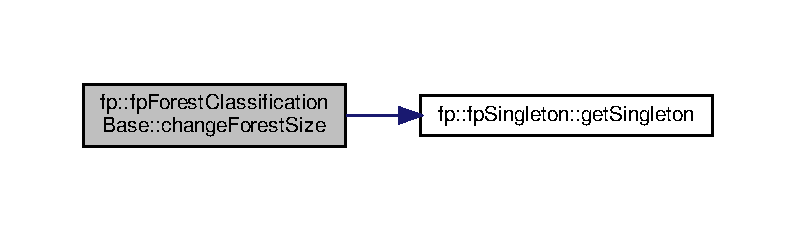
\includegraphics[width=350pt]{classfp_1_1fpForestClassificationBase_a696b361df0a1c9aa36687333e2d8111b_cgraph}
\end{center}
\end{figure}
\mbox{\Hypertarget{classfp_1_1fpForestClassificationBase_a3186e3b6471f82df3f69172f67aa7d19}\label{classfp_1_1fpForestClassificationBase_a3186e3b6471f82df3f69172f67aa7d19}} 
\index{fp\+::fp\+Forest\+Classification\+Base@{fp\+::fp\+Forest\+Classification\+Base}!check\+Parameters@{check\+Parameters}}
\index{check\+Parameters@{check\+Parameters}!fp\+::fp\+Forest\+Classification\+Base@{fp\+::fp\+Forest\+Classification\+Base}}
\subsubsection{\texorpdfstring{check\+Parameters()}{checkParameters()}}
{\footnotesize\ttfamily template$<$typename T $>$ \\
void \hyperlink{classfp_1_1fpForestClassificationBase}{fp\+::fp\+Forest\+Classification\+Base}$<$ T $>$\+::check\+Parameters (\begin{DoxyParamCaption}{ }\end{DoxyParamCaption})\hspace{0.3cm}{\ttfamily [inline]}}



Definition at line 45 of file fp\+Forest\+Classification\+Base.\+h.


\begin{DoxyCode}
45                                          \{
46                 \textcolor{comment}{//TODO: check parameters to make sure they make sense for this forest type.}
47                 ;
48             \}
\end{DoxyCode}
\mbox{\Hypertarget{classfp_1_1fpForestClassificationBase_a706225fdbef8c71fb022f4c3446b388d}\label{classfp_1_1fpForestClassificationBase_a706225fdbef8c71fb022f4c3446b388d}} 
\index{fp\+::fp\+Forest\+Classification\+Base@{fp\+::fp\+Forest\+Classification\+Base}!grow\+Forest@{grow\+Forest}}
\index{grow\+Forest@{grow\+Forest}!fp\+::fp\+Forest\+Classification\+Base@{fp\+::fp\+Forest\+Classification\+Base}}
\subsubsection{\texorpdfstring{grow\+Forest()}{growForest()}}
{\footnotesize\ttfamily template$<$typename T $>$ \\
void \hyperlink{classfp_1_1fpForestClassificationBase}{fp\+::fp\+Forest\+Classification\+Base}$<$ T $>$\+::grow\+Forest (\begin{DoxyParamCaption}{ }\end{DoxyParamCaption})\hspace{0.3cm}{\ttfamily [inline]}, {\ttfamily [virtual]}}



Implements \hyperlink{classfp_1_1fpForestBase_a05b1d924a559536083ee7a8cf3ea542d}{fp\+::fp\+Forest\+Base}.



Definition at line 73 of file fp\+Forest\+Classification\+Base.\+h.


\begin{DoxyCode}
73                              \{
74                 \textcolor{comment}{//  checkParameters();}
75                 \hyperlink{classfp_1_1fpForestClassificationBase_a696b361df0a1c9aa36687333e2d8111b}{changeForestSize}();
76                 \hyperlink{classfp_1_1fpForestClassificationBase_aea9db2571269f0f627226aa75ec4a694}{growTrees}();
77                 \hyperlink{classfp_1_1fpForestClassificationBase_a48567d379434daeccb1540c84674d286}{treeStats}();
78             \}
\end{DoxyCode}
Here is the call graph for this function\+:
\nopagebreak
\begin{figure}[H]
\begin{center}
\leavevmode
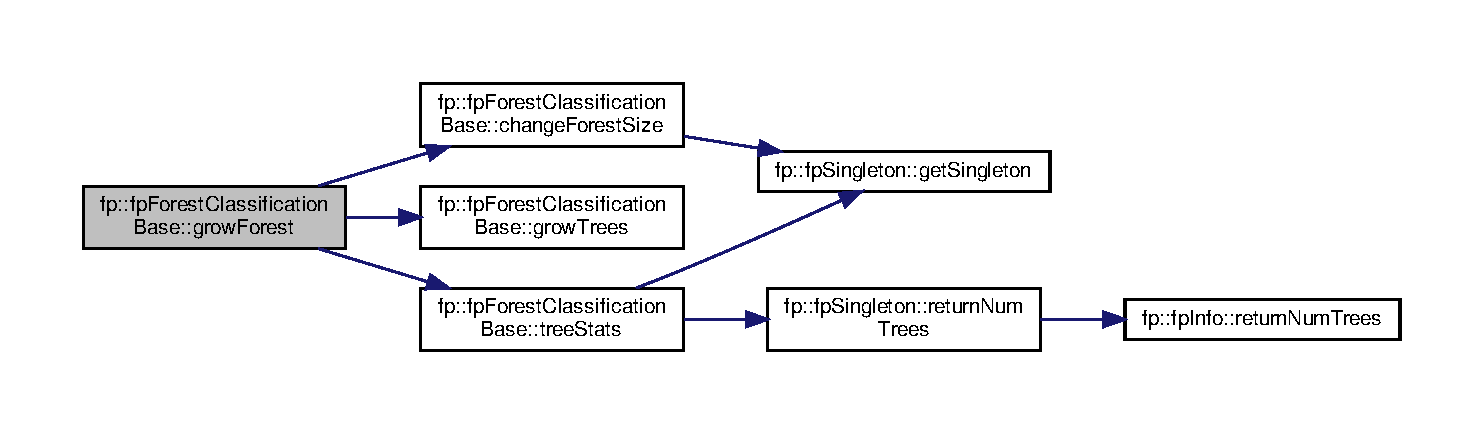
\includegraphics[width=350pt]{classfp_1_1fpForestClassificationBase_a706225fdbef8c71fb022f4c3446b388d_cgraph}
\end{center}
\end{figure}
\mbox{\Hypertarget{classfp_1_1fpForestClassificationBase_aea9db2571269f0f627226aa75ec4a694}\label{classfp_1_1fpForestClassificationBase_aea9db2571269f0f627226aa75ec4a694}} 
\index{fp\+::fp\+Forest\+Classification\+Base@{fp\+::fp\+Forest\+Classification\+Base}!grow\+Trees@{grow\+Trees}}
\index{grow\+Trees@{grow\+Trees}!fp\+::fp\+Forest\+Classification\+Base@{fp\+::fp\+Forest\+Classification\+Base}}
\subsubsection{\texorpdfstring{grow\+Trees()}{growTrees()}}
{\footnotesize\ttfamily template$<$typename T $>$ \\
void \hyperlink{classfp_1_1fpForestClassificationBase}{fp\+::fp\+Forest\+Classification\+Base}$<$ T $>$\+::grow\+Trees (\begin{DoxyParamCaption}{ }\end{DoxyParamCaption})\hspace{0.3cm}{\ttfamily [inline]}}



Definition at line 36 of file fp\+Forest\+Classification\+Base.\+h.


\begin{DoxyCode}
36                             \{
37 
38                 \textcolor{keywordflow}{for}(\textcolor{keywordtype}{unsigned} \textcolor{keywordtype}{int} i = 0; i < \hyperlink{classfp_1_1fpForestClassificationBase_a51482a6c95c4b3cb42627f029c2d4662}{trees}.size(); ++i)\{
39                     \hyperlink{classfp_1_1fpForestClassificationBase_a21148775a113092d6929e0d28e351a2c}{printProgress}.\hyperlink{classfp_1_1fpDisplayProgress_adf5b2e390618d63eccb6de3b00eb857b}{displayProgress}(i);
40                     \hyperlink{classfp_1_1fpForestClassificationBase_a51482a6c95c4b3cb42627f029c2d4662}{trees}[i].growTree();
41                 \}
42                 std::cout << \textcolor{stringliteral}{"\(\backslash\)n"}<< std::flush;
43             \}
\end{DoxyCode}
Here is the call graph for this function\+:
\nopagebreak
\begin{figure}[H]
\begin{center}
\leavevmode
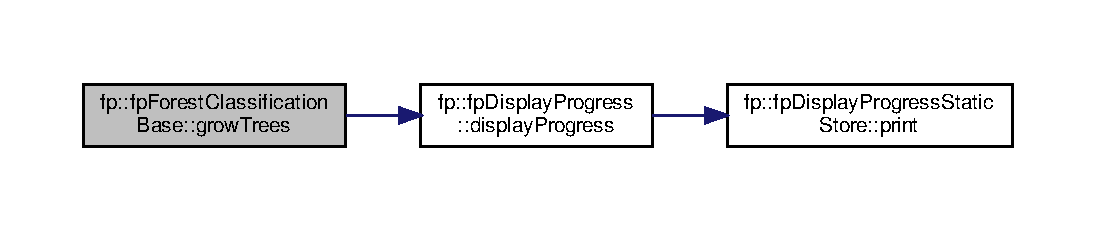
\includegraphics[width=350pt]{classfp_1_1fpForestClassificationBase_aea9db2571269f0f627226aa75ec4a694_cgraph}
\end{center}
\end{figure}
\mbox{\Hypertarget{classfp_1_1fpForestClassificationBase_ad0c690fff971fab681467fbcd8762b5f}\label{classfp_1_1fpForestClassificationBase_ad0c690fff971fab681467fbcd8762b5f}} 
\index{fp\+::fp\+Forest\+Classification\+Base@{fp\+::fp\+Forest\+Classification\+Base}!predict\+Class@{predict\+Class}}
\index{predict\+Class@{predict\+Class}!fp\+::fp\+Forest\+Classification\+Base@{fp\+::fp\+Forest\+Classification\+Base}}
\subsubsection{\texorpdfstring{predict\+Class()}{predictClass()}}
{\footnotesize\ttfamily template$<$typename T $>$ \\
int \hyperlink{classfp_1_1fpForestClassificationBase}{fp\+::fp\+Forest\+Classification\+Base}$<$ T $>$\+::predict\+Class (\begin{DoxyParamCaption}\item[{int}]{observation\+Number }\end{DoxyParamCaption})\hspace{0.3cm}{\ttfamily [inline]}}



Definition at line 80 of file fp\+Forest\+Classification\+Base.\+h.


\begin{DoxyCode}
80                                                    \{
81                 std::vector<int> classTally(\hyperlink{classfp_1_1fpSingleton_a8bdae77b68521003e3fc630edec2e240}{fpSingleton::getSingleton}().
      returnNumClasses(),0);
82                 \textcolor{keywordflow}{for}(\textcolor{keywordtype}{int} i = 0; i < \hyperlink{classfp_1_1fpSingleton_a8bdae77b68521003e3fc630edec2e240}{fpSingleton::getSingleton}().
      \hyperlink{classfp_1_1fpSingleton_a8be36616345b6b77ce4c60b99cc2b91c}{returnNumTrees}(); ++i)\{
83                     ++classTally[\hyperlink{classfp_1_1fpForestClassificationBase_a51482a6c95c4b3cb42627f029c2d4662}{trees}[i].predictObservation(observationNumber)];
84                 \}
85 
86                 \textcolor{keywordtype}{int} bestClass = 0;
87                 \textcolor{keywordflow}{for}(\textcolor{keywordtype}{int} j = 1; j < \hyperlink{classfp_1_1fpSingleton_a8bdae77b68521003e3fc630edec2e240}{fpSingleton::getSingleton}().
      \hyperlink{classfp_1_1fpSingleton_a5602580110329a6b25602b1789e4e2c2}{returnNumClasses}(); ++j)\{
88                     \textcolor{keywordflow}{if}(classTally[bestClass] < classTally[j])\{
89                         bestClass = j;
90                     \}
91                 \}
92                 \textcolor{keywordflow}{return} bestClass;
93             \}
\end{DoxyCode}
Here is the call graph for this function\+:
\nopagebreak
\begin{figure}[H]
\begin{center}
\leavevmode
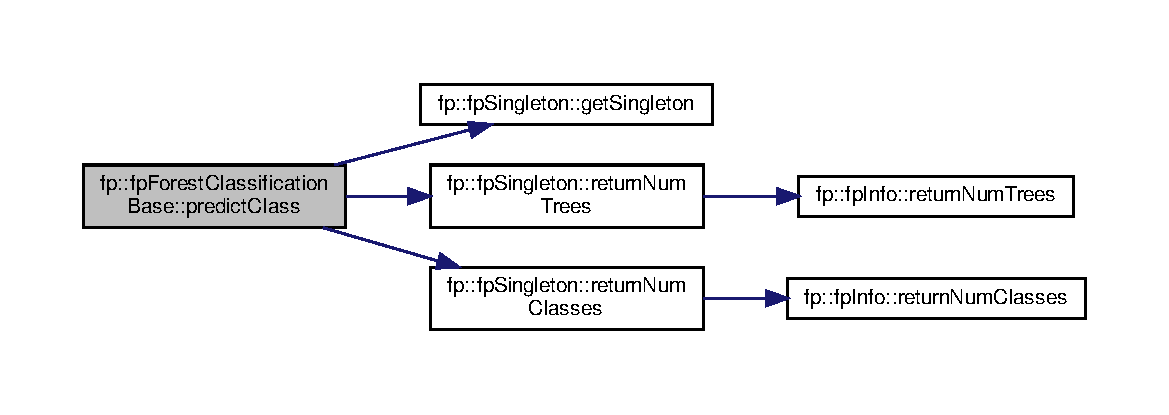
\includegraphics[width=350pt]{classfp_1_1fpForestClassificationBase_ad0c690fff971fab681467fbcd8762b5f_cgraph}
\end{center}
\end{figure}
\mbox{\Hypertarget{classfp_1_1fpForestClassificationBase_a6b5243d32b468308a4f013ad5a9df2dd}\label{classfp_1_1fpForestClassificationBase_a6b5243d32b468308a4f013ad5a9df2dd}} 
\index{fp\+::fp\+Forest\+Classification\+Base@{fp\+::fp\+Forest\+Classification\+Base}!print\+Forest\+Type@{print\+Forest\+Type}}
\index{print\+Forest\+Type@{print\+Forest\+Type}!fp\+::fp\+Forest\+Classification\+Base@{fp\+::fp\+Forest\+Classification\+Base}}
\subsubsection{\texorpdfstring{print\+Forest\+Type()}{printForestType()}}
{\footnotesize\ttfamily template$<$typename T $>$ \\
void \hyperlink{classfp_1_1fpForestClassificationBase}{fp\+::fp\+Forest\+Classification\+Base}$<$ T $>$\+::print\+Forest\+Type (\begin{DoxyParamCaption}{ }\end{DoxyParamCaption})\hspace{0.3cm}{\ttfamily [inline]}, {\ttfamily [virtual]}}



Implements \hyperlink{classfp_1_1fpForestBase_a5e200f603cca94bb5d9f357489f07e97}{fp\+::fp\+Forest\+Base}.



Definition at line 28 of file fp\+Forest\+Classification\+Base.\+h.


\begin{DoxyCode}
28                                   \{
29                 std::cout << \textcolor{stringliteral}{"This is a basic classification forest.\(\backslash\)n"};
30             \}
\end{DoxyCode}
\mbox{\Hypertarget{classfp_1_1fpForestClassificationBase_a1989f90fbd27ac90232b7a1071c96a00}\label{classfp_1_1fpForestClassificationBase_a1989f90fbd27ac90232b7a1071c96a00}} 
\index{fp\+::fp\+Forest\+Classification\+Base@{fp\+::fp\+Forest\+Classification\+Base}!print\+Tree0@{print\+Tree0}}
\index{print\+Tree0@{print\+Tree0}!fp\+::fp\+Forest\+Classification\+Base@{fp\+::fp\+Forest\+Classification\+Base}}
\subsubsection{\texorpdfstring{print\+Tree0()}{printTree0()}}
{\footnotesize\ttfamily template$<$typename T $>$ \\
void \hyperlink{classfp_1_1fpForestClassificationBase}{fp\+::fp\+Forest\+Classification\+Base}$<$ T $>$\+::print\+Tree0 (\begin{DoxyParamCaption}{ }\end{DoxyParamCaption})\hspace{0.3cm}{\ttfamily [inline]}}



Definition at line 69 of file fp\+Forest\+Classification\+Base.\+h.


\begin{DoxyCode}
69                              \{
70                 \hyperlink{classfp_1_1fpForestClassificationBase_a51482a6c95c4b3cb42627f029c2d4662}{trees}[0].printTree();
71             \}
\end{DoxyCode}
\mbox{\Hypertarget{classfp_1_1fpForestClassificationBase_a3f1ad5a5cfb3633713d0a81bd1c356e8}\label{classfp_1_1fpForestClassificationBase_a3f1ad5a5cfb3633713d0a81bd1c356e8}} 
\index{fp\+::fp\+Forest\+Classification\+Base@{fp\+::fp\+Forest\+Classification\+Base}!test\+Forest@{test\+Forest}}
\index{test\+Forest@{test\+Forest}!fp\+::fp\+Forest\+Classification\+Base@{fp\+::fp\+Forest\+Classification\+Base}}
\subsubsection{\texorpdfstring{test\+Forest()}{testForest()}}
{\footnotesize\ttfamily template$<$typename T $>$ \\
float \hyperlink{classfp_1_1fpForestClassificationBase}{fp\+::fp\+Forest\+Classification\+Base}$<$ T $>$\+::test\+Forest (\begin{DoxyParamCaption}{ }\end{DoxyParamCaption})\hspace{0.3cm}{\ttfamily [inline]}, {\ttfamily [virtual]}}



Implements \hyperlink{classfp_1_1fpForestBase_af7becba028a198f650841b718d16ed16}{fp\+::fp\+Forest\+Base}.



Definition at line 96 of file fp\+Forest\+Classification\+Base.\+h.


\begin{DoxyCode}
96                               \{
97                 \textcolor{keywordtype}{float} numTried = 0;
98                 \textcolor{keywordtype}{float} numWrong = 0;
99 
100                 \textcolor{keywordflow}{for} (\textcolor{keywordtype}{int} i = 0; i <\hyperlink{classfp_1_1fpSingleton_a8bdae77b68521003e3fc630edec2e240}{fpSingleton::getSingleton}().
      \hyperlink{classfp_1_1fpSingleton_ae0a2963feb07b809b8740218f1048b67}{returnNumObservations}();i++)\{
101                     ++numTried;
102                     \textcolor{keywordtype}{int} predClass = \hyperlink{classfp_1_1fpForestClassificationBase_ad0c690fff971fab681467fbcd8762b5f}{predictClass}(i);
103 
104                     \textcolor{keywordflow}{if}(predClass != \hyperlink{classfp_1_1fpSingleton_a8bdae77b68521003e3fc630edec2e240}{fpSingleton::getSingleton}().returnTestLabel(i)
      )\{
105                         ++numWrong;
106                     \}
107                 \}
108                 std::cout << \textcolor{stringliteral}{"\(\backslash\)nnumWrong= "} << numWrong << \textcolor{stringliteral}{"\(\backslash\)n"};
109 
110                 \textcolor{keywordflow}{return} numWrong/numTried;
111             \}
\end{DoxyCode}
Here is the call graph for this function\+:
\nopagebreak
\begin{figure}[H]
\begin{center}
\leavevmode
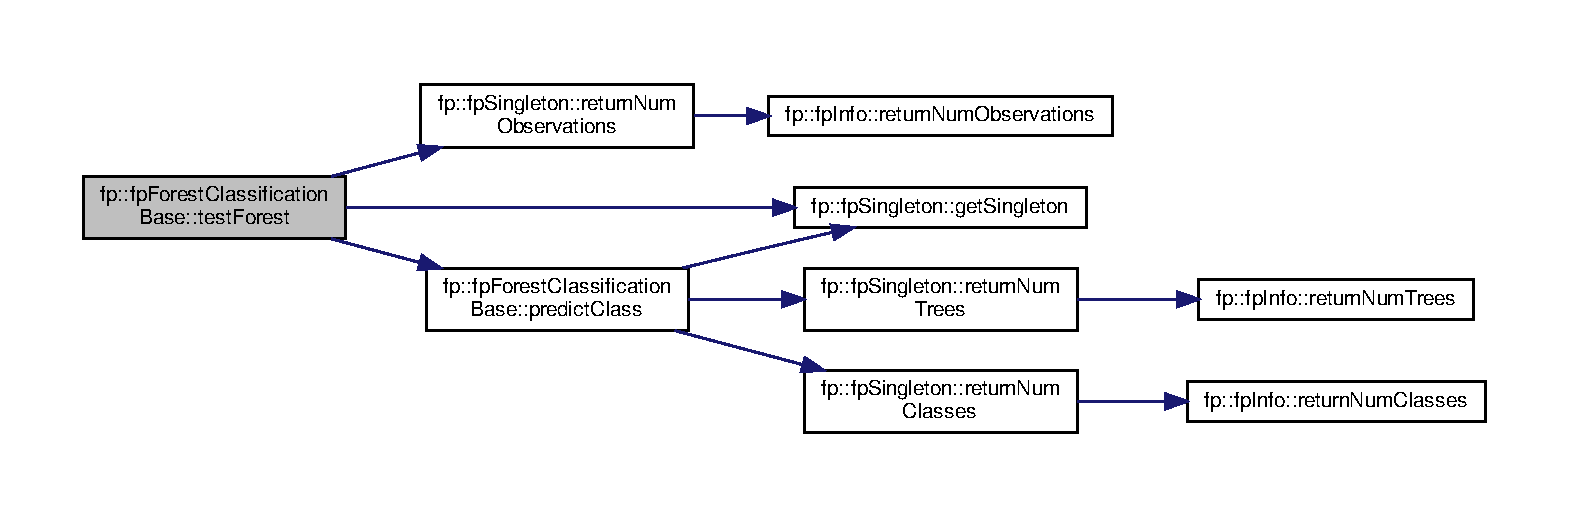
\includegraphics[width=350pt]{classfp_1_1fpForestClassificationBase_a3f1ad5a5cfb3633713d0a81bd1c356e8_cgraph}
\end{center}
\end{figure}
\mbox{\Hypertarget{classfp_1_1fpForestClassificationBase_a48567d379434daeccb1540c84674d286}\label{classfp_1_1fpForestClassificationBase_a48567d379434daeccb1540c84674d286}} 
\index{fp\+::fp\+Forest\+Classification\+Base@{fp\+::fp\+Forest\+Classification\+Base}!tree\+Stats@{tree\+Stats}}
\index{tree\+Stats@{tree\+Stats}!fp\+::fp\+Forest\+Classification\+Base@{fp\+::fp\+Forest\+Classification\+Base}}
\subsubsection{\texorpdfstring{tree\+Stats()}{treeStats()}}
{\footnotesize\ttfamily template$<$typename T $>$ \\
void \hyperlink{classfp_1_1fpForestClassificationBase}{fp\+::fp\+Forest\+Classification\+Base}$<$ T $>$\+::tree\+Stats (\begin{DoxyParamCaption}{ }\end{DoxyParamCaption})\hspace{0.3cm}{\ttfamily [inline]}}



Definition at line 50 of file fp\+Forest\+Classification\+Base.\+h.


\begin{DoxyCode}
50                             \{
51                 \textcolor{keywordtype}{int} maxDepth=0;
52                 \textcolor{keywordtype}{int} totalLeafNodes=0;
53                 \textcolor{keywordtype}{int} totalLeafDepth=0;
54 
55                 \textcolor{keywordtype}{int} tempMaxDepth;
56                 \textcolor{keywordflow}{for}(\textcolor{keywordtype}{int} i = 0; i < \hyperlink{classfp_1_1fpSingleton_a8bdae77b68521003e3fc630edec2e240}{fpSingleton::getSingleton}().
      \hyperlink{classfp_1_1fpSingleton_a8be36616345b6b77ce4c60b99cc2b91c}{returnNumTrees}(); ++i)\{
57                     tempMaxDepth = \hyperlink{classfp_1_1fpForestClassificationBase_a51482a6c95c4b3cb42627f029c2d4662}{trees}[i].returnMaxDepth();
58                     maxDepth = ((maxDepth < tempMaxDepth) ? tempMaxDepth : maxDepth);
59 
60                     totalLeafNodes += \hyperlink{classfp_1_1fpForestClassificationBase_a51482a6c95c4b3cb42627f029c2d4662}{trees}[i].returnNumLeafNodes();
61                     totalLeafDepth += \hyperlink{classfp_1_1fpForestClassificationBase_a51482a6c95c4b3cb42627f029c2d4662}{trees}[i].returnLeafDepthSum();
62                 \}
63 
64                 std::cout << \textcolor{stringliteral}{"max depth: "} << maxDepth << \textcolor{stringliteral}{"\(\backslash\)n"};
65                 std::cout << \textcolor{stringliteral}{"avg depth: "} << float(totalLeafDepth)/float(totalLeafNodes) << \textcolor{stringliteral}{"\(\backslash\)n"};
66                 std::cout << \textcolor{stringliteral}{"num leaf nodes: "} << totalLeafNodes << \textcolor{stringliteral}{"\(\backslash\)n"};
67             \}
\end{DoxyCode}
Here is the call graph for this function\+:
\nopagebreak
\begin{figure}[H]
\begin{center}
\leavevmode
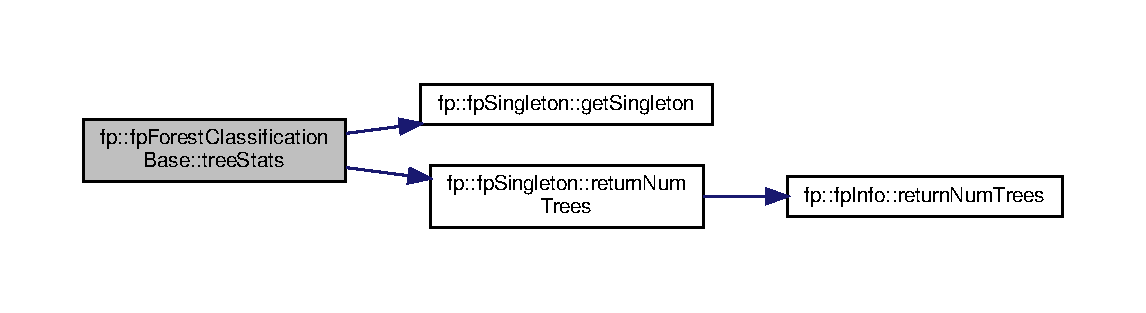
\includegraphics[width=350pt]{classfp_1_1fpForestClassificationBase_a48567d379434daeccb1540c84674d286_cgraph}
\end{center}
\end{figure}


\subsection{Member Data Documentation}
\mbox{\Hypertarget{classfp_1_1fpForestClassificationBase_a21148775a113092d6929e0d28e351a2c}\label{classfp_1_1fpForestClassificationBase_a21148775a113092d6929e0d28e351a2c}} 
\index{fp\+::fp\+Forest\+Classification\+Base@{fp\+::fp\+Forest\+Classification\+Base}!print\+Progress@{print\+Progress}}
\index{print\+Progress@{print\+Progress}!fp\+::fp\+Forest\+Classification\+Base@{fp\+::fp\+Forest\+Classification\+Base}}
\subsubsection{\texorpdfstring{print\+Progress}{printProgress}}
{\footnotesize\ttfamily template$<$typename T $>$ \\
\hyperlink{classfp_1_1fpDisplayProgress}{fp\+Display\+Progress} \hyperlink{classfp_1_1fpForestClassificationBase}{fp\+::fp\+Forest\+Classification\+Base}$<$ T $>$\+::print\+Progress}



Definition at line 22 of file fp\+Forest\+Classification\+Base.\+h.

\mbox{\Hypertarget{classfp_1_1fpForestClassificationBase_a51482a6c95c4b3cb42627f029c2d4662}\label{classfp_1_1fpForestClassificationBase_a51482a6c95c4b3cb42627f029c2d4662}} 
\index{fp\+::fp\+Forest\+Classification\+Base@{fp\+::fp\+Forest\+Classification\+Base}!trees@{trees}}
\index{trees@{trees}!fp\+::fp\+Forest\+Classification\+Base@{fp\+::fp\+Forest\+Classification\+Base}}
\subsubsection{\texorpdfstring{trees}{trees}}
{\footnotesize\ttfamily template$<$typename T $>$ \\
std\+::vector$<$\hyperlink{classfp_1_1rfTree}{rf\+Tree}$<$T$>$ $>$ \hyperlink{classfp_1_1fpForestClassificationBase}{fp\+::fp\+Forest\+Classification\+Base}$<$ T $>$\+::trees\hspace{0.3cm}{\ttfamily [protected]}}



Definition at line 19 of file fp\+Forest\+Classification\+Base.\+h.



The documentation for this class was generated from the following file\+:\begin{DoxyCompactItemize}
\item 
src/forest\+Types/rf\+Classification/\hyperlink{fpForestClassificationBase_8h}{fp\+Forest\+Classification\+Base.\+h}\end{DoxyCompactItemize}

\hypertarget{classfp_1_1fpGrowingTree}{}\section{fp\+:\+:fp\+Growing\+Tree$<$ T $>$ Class Template Reference}
\label{classfp_1_1fpGrowingTree}\index{fp\+::fp\+Growing\+Tree$<$ T $>$@{fp\+::fp\+Growing\+Tree$<$ T $>$}}


{\ttfamily \#include $<$fp\+Growing\+Tree.\+h$>$}

\subsection*{Public Member Functions}
\begin{DoxyCompactItemize}
\item 
\hyperlink{classfp_1_1fpGrowingTree_a7704cdb870c23913b5247de052f2c635}{fp\+Growing\+Tree} ()
\item 
\hyperlink{classfp_1_1fpGrowingTree_a5762c272db68e2e28c767053f752418f}{initialize\+Root\+Of\+Tree} (int growing\+Tree\+Number)
\end{DoxyCompactItemize}
\subsection*{Protected Attributes}
\begin{DoxyCompactItemize}
\item 
std\+::vector$<$ \hyperlink{classfp_1_1growingTreeElement}{growing\+Tree\+Element}$<$ T $>$ $>$ \hyperlink{classfp_1_1fpGrowingTree_ad729a18d4cd23d38a5bcab4bdd1ed58b}{node\+Index\+Holder}
\item 
std\+::vector$<$ int $>$ \hyperlink{classfp_1_1fpGrowingTree_afdd5b18a4e4f282e3c5aba30caf918c0}{O\+O\+B\+Holder}
\end{DoxyCompactItemize}


\subsection{Detailed Description}
\subsubsection*{template$<$typename T$>$\newline
class fp\+::fp\+Growing\+Tree$<$ T $>$}



Definition at line 11 of file fp\+Growing\+Tree.\+h.



\subsection{Constructor \& Destructor Documentation}
\mbox{\Hypertarget{classfp_1_1fpGrowingTree_a7704cdb870c23913b5247de052f2c635}\label{classfp_1_1fpGrowingTree_a7704cdb870c23913b5247de052f2c635}} 
\index{fp\+::fp\+Growing\+Tree@{fp\+::fp\+Growing\+Tree}!fp\+Growing\+Tree@{fp\+Growing\+Tree}}
\index{fp\+Growing\+Tree@{fp\+Growing\+Tree}!fp\+::fp\+Growing\+Tree@{fp\+::fp\+Growing\+Tree}}
\subsubsection{\texorpdfstring{fp\+Growing\+Tree()}{fpGrowingTree()}}
{\footnotesize\ttfamily template$<$typename T $>$ \\
\hyperlink{classfp_1_1fpGrowingTree}{fp\+::fp\+Growing\+Tree}$<$ T $>$\+::\hyperlink{classfp_1_1fpGrowingTree}{fp\+Growing\+Tree} (\begin{DoxyParamCaption}{ }\end{DoxyParamCaption})\hspace{0.3cm}{\ttfamily [inline]}}



Definition at line 18 of file fp\+Growing\+Tree.\+h.


\begin{DoxyCode}
18                                \{
19             \hyperlink{classfp_1_1fpGrowingTree_ad729a18d4cd23d38a5bcab4bdd1ed58b}{nodeIndexHolder}.resize(\hyperlink{classfp_1_1fpSingleton_a8bdae77b68521003e3fc630edec2e240}{fpSingleton::getSingleton}().
      returnNumObservations());    
20             \hyperlink{classfp_1_1fpGrowingTree_afdd5b18a4e4f282e3c5aba30caf918c0}{OOBHolder}.resize(\hyperlink{classfp_1_1fpSingleton_a8bdae77b68521003e3fc630edec2e240}{fpSingleton::getSingleton}().
      returnNumObservations()/2);  
21                 \}
\end{DoxyCode}
Here is the call graph for this function\+:
\nopagebreak
\begin{figure}[H]
\begin{center}
\leavevmode
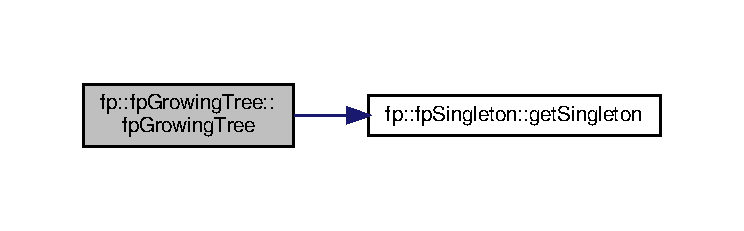
\includegraphics[width=350pt]{classfp_1_1fpGrowingTree_a7704cdb870c23913b5247de052f2c635_cgraph}
\end{center}
\end{figure}


\subsection{Member Function Documentation}
\mbox{\Hypertarget{classfp_1_1fpGrowingTree_a5762c272db68e2e28c767053f752418f}\label{classfp_1_1fpGrowingTree_a5762c272db68e2e28c767053f752418f}} 
\index{fp\+::fp\+Growing\+Tree@{fp\+::fp\+Growing\+Tree}!initialize\+Root\+Of\+Tree@{initialize\+Root\+Of\+Tree}}
\index{initialize\+Root\+Of\+Tree@{initialize\+Root\+Of\+Tree}!fp\+::fp\+Growing\+Tree@{fp\+::fp\+Growing\+Tree}}
\subsubsection{\texorpdfstring{initialize\+Root\+Of\+Tree()}{initializeRootOfTree()}}
{\footnotesize\ttfamily template$<$typename T $>$ \\
\hyperlink{classfp_1_1fpGrowingTree}{fp\+::fp\+Growing\+Tree}$<$ T $>$\+::initialize\+Root\+Of\+Tree (\begin{DoxyParamCaption}\item[{int}]{growing\+Tree\+Number }\end{DoxyParamCaption})\hspace{0.3cm}{\ttfamily [inline]}}



Definition at line 23 of file fp\+Growing\+Tree.\+h.


\begin{DoxyCode}
23                                                                   \{
24 
25 
26                 \}
\end{DoxyCode}


\subsection{Member Data Documentation}
\mbox{\Hypertarget{classfp_1_1fpGrowingTree_ad729a18d4cd23d38a5bcab4bdd1ed58b}\label{classfp_1_1fpGrowingTree_ad729a18d4cd23d38a5bcab4bdd1ed58b}} 
\index{fp\+::fp\+Growing\+Tree@{fp\+::fp\+Growing\+Tree}!node\+Index\+Holder@{node\+Index\+Holder}}
\index{node\+Index\+Holder@{node\+Index\+Holder}!fp\+::fp\+Growing\+Tree@{fp\+::fp\+Growing\+Tree}}
\subsubsection{\texorpdfstring{node\+Index\+Holder}{nodeIndexHolder}}
{\footnotesize\ttfamily template$<$typename T $>$ \\
std\+::vector$<$\hyperlink{classfp_1_1growingTreeElement}{growing\+Tree\+Element}$<$T$>$ $>$ \hyperlink{classfp_1_1fpGrowingTree}{fp\+::fp\+Growing\+Tree}$<$ T $>$\+::node\+Index\+Holder\hspace{0.3cm}{\ttfamily [protected]}}



Definition at line 14 of file fp\+Growing\+Tree.\+h.

\mbox{\Hypertarget{classfp_1_1fpGrowingTree_afdd5b18a4e4f282e3c5aba30caf918c0}\label{classfp_1_1fpGrowingTree_afdd5b18a4e4f282e3c5aba30caf918c0}} 
\index{fp\+::fp\+Growing\+Tree@{fp\+::fp\+Growing\+Tree}!O\+O\+B\+Holder@{O\+O\+B\+Holder}}
\index{O\+O\+B\+Holder@{O\+O\+B\+Holder}!fp\+::fp\+Growing\+Tree@{fp\+::fp\+Growing\+Tree}}
\subsubsection{\texorpdfstring{O\+O\+B\+Holder}{OOBHolder}}
{\footnotesize\ttfamily template$<$typename T $>$ \\
std\+::vector$<$int$>$ \hyperlink{classfp_1_1fpGrowingTree}{fp\+::fp\+Growing\+Tree}$<$ T $>$\+::O\+O\+B\+Holder\hspace{0.3cm}{\ttfamily [protected]}}



Definition at line 15 of file fp\+Growing\+Tree.\+h.



The documentation for this class was generated from the following file\+:\begin{DoxyCompactItemize}
\item 
src/base\+Functions/fp\+Growing\+Tree\+Helpers/\hyperlink{fpGrowingTree_8h}{fp\+Growing\+Tree.\+h}\end{DoxyCompactItemize}

\hypertarget{classfp_1_1fpInfo}{}\section{fp\+:\+:fp\+Info Class Reference}
\label{classfp_1_1fpInfo}\index{fp\+::fp\+Info@{fp\+::fp\+Info}}


{\ttfamily \#include $<$fp\+Info.\+h$>$}

\subsection*{Public Member Functions}
\begin{DoxyCompactItemize}
\item 
\hyperlink{classfp_1_1fpInfo_a2a0f7c8215dd138b690efe8a03484aef}{fp\+Info} ()
\item 
void \hyperlink{classfp_1_1fpInfo_ae4c749c466e983cb312cc08d38b2796e}{set\+Parameter} (const std\+::string \&parameter\+Name, const std\+::string \&parameter\+Value)
\item 
void \hyperlink{classfp_1_1fpInfo_a8ef4332ee98a1724ffd8614c4f80af91}{set\+Parameter} (const std\+::string \&parameter\+Name, const double parameter\+Value)
\item 
void \hyperlink{classfp_1_1fpInfo_aa2dd574c5a3764c250f1ccb1b11de1e0}{set\+Parameter} (const std\+::string \&parameter\+Name, const int parameter\+Value)
\item 
void \hyperlink{classfp_1_1fpInfo_a471bd46c828547d5b556f6f4e9fca70f}{print\+All\+Parameters} ()
\item 
void \hyperlink{classfp_1_1fpInfo_a1acfffe3b13e5cad548f92cd09ff7f46}{print\+Forest\+Type} ()
\item 
std\+::string \& \hyperlink{classfp_1_1fpInfo_a78c57a1955263d343c794f2156cd0a76}{return\+C\+S\+V\+File\+Name} ()
\item 
std\+::string \& \hyperlink{classfp_1_1fpInfo_a97280e7e3cadc5e653d8ef256eb2c82d}{return\+Forest\+Type} ()
\item 
int \hyperlink{classfp_1_1fpInfo_a52ef3c184d39133dae472bb51e1287e7}{return\+Column\+WithY} ()
\item 
int \hyperlink{classfp_1_1fpInfo_a641516fa21a5d6170f74426cf9e2b255}{return\+Num\+Classes} ()
\item 
int \hyperlink{classfp_1_1fpInfo_ad1af845e85cb6e807694c5106baca230}{return\+Min\+Parent} ()
\item 
int \hyperlink{classfp_1_1fpInfo_abf1e1bfc3e7daa178f3d68bed6311edb}{return\+Num\+Features} ()
\item 
int \hyperlink{classfp_1_1fpInfo_a5d70dfbd1f8dc26dbd8f066e210cf165}{return\+Num\+Observations} ()
\item 
void \hyperlink{classfp_1_1fpInfo_a3598d1ab13bf05b53858b1ca8c44fa68}{set\+Num\+Classes} (int numC)
\item 
void \hyperlink{classfp_1_1fpInfo_a69ef99f2ec9ef74dd3787bc33ffb05d0}{set\+Num\+Features} (int numF)
\item 
void \hyperlink{classfp_1_1fpInfo_ad17492e79df7bca55d98438fec2f004b}{set\+Num\+Observations} (int numO)
\item 
int \hyperlink{classfp_1_1fpInfo_a12d3d4b2216f37daf6555f07148c4f85}{return\+Num\+Trees} ()
\item 
bool \hyperlink{classfp_1_1fpInfo_a2a6ac3cfea5db5842baa1789468492ad}{load\+Data\+From\+C\+SV} ()
\item 
int \hyperlink{classfp_1_1fpInfo_a058477c4f05818c220efa469b7b630bb}{return\+Mtry} ()
\item 
bool \hyperlink{classfp_1_1fpInfo_a0a00d3d54cef667000249202a2d768bf}{use\+Default\+M\+T\+RY} ()
\item 
void \hyperlink{classfp_1_1fpInfo_a6b2a54fb9b3672e7b1bab3474a0ca33f}{set\+M\+T\+RY} ()
\end{DoxyCompactItemize}
\subsection*{Protected Attributes}
\begin{DoxyCompactItemize}
\item 
int \hyperlink{classfp_1_1fpInfo_a8dbd62dca5c972c29d29a69d90ca2632}{num\+Trees\+In\+Forest}
\item 
int \hyperlink{classfp_1_1fpInfo_a128fab7ba6da0fc76da00b48bb1bd7d5}{min\+Parent} = 1
\item 
int \hyperlink{classfp_1_1fpInfo_a1c98a9ced12230f21003f78d742625a3}{num\+Classes} = -\/1
\item 
int \hyperlink{classfp_1_1fpInfo_a1b35cd17d4ddb35e232246a6549d7a74}{num\+Observations} = -\/1
\item 
int \hyperlink{classfp_1_1fpInfo_a6ed8deabebae772fc213730cd29a2e61}{num\+Features} = -\/1
\item 
int \hyperlink{classfp_1_1fpInfo_a62cccc1eb5641ebec2a6cc86cf03eedf}{mtry} = -\/1
\item 
int \hyperlink{classfp_1_1fpInfo_ac29e135cd84cdef547b678e7ea37f92d}{column\+WithY} = -\/1
\item 
int \hyperlink{classfp_1_1fpInfo_a9404de3ad49dc78e3d5c8e3ef8b04fba}{number\+Of\+Nodes}
\item 
int \hyperlink{classfp_1_1fpInfo_a95c744fa049788dd61fa0fccdec4565d}{max\+Depth}
\item 
int \hyperlink{classfp_1_1fpInfo_a13afa17097728f059e8525ea382b71cd}{sum\+Leaf\+Node\+Depths}
\item 
double \hyperlink{classfp_1_1fpInfo_ab949cb97523283367e9b120fd78e3c3b}{fraction\+Of\+Features\+To\+Test} = -\/1.\+0
\item 
std\+::string \hyperlink{classfp_1_1fpInfo_a3001fbf80d86022e53578d6adf133b90}{forest\+Type}
\item 
std\+::string \hyperlink{classfp_1_1fpInfo_aac01e5ddb27bc333e172a0422066af1c}{C\+S\+V\+File\+Name}
\end{DoxyCompactItemize}


\subsection{Detailed Description}


Definition at line 11 of file fp\+Info.\+h.



\subsection{Constructor \& Destructor Documentation}
\mbox{\Hypertarget{classfp_1_1fpInfo_a2a0f7c8215dd138b690efe8a03484aef}\label{classfp_1_1fpInfo_a2a0f7c8215dd138b690efe8a03484aef}} 
\index{fp\+::fp\+Info@{fp\+::fp\+Info}!fp\+Info@{fp\+Info}}
\index{fp\+Info@{fp\+Info}!fp\+::fp\+Info@{fp\+::fp\+Info}}
\subsubsection{\texorpdfstring{fp\+Info()}{fpInfo()}}
{\footnotesize\ttfamily fp\+::fp\+Info\+::fp\+Info (\begin{DoxyParamCaption}{ }\end{DoxyParamCaption})}



Definition at line 7 of file fp\+Info.\+cpp.


\begin{DoxyCode}
7                   : \hyperlink{classfp_1_1fpInfo_a8dbd62dca5c972c29d29a69d90ca2632}{numTreesInForest}(100),
8     \hyperlink{classfp_1_1fpInfo_a128fab7ba6da0fc76da00b48bb1bd7d5}{minParent}(1),  \hyperlink{classfp_1_1fpInfo_a1c98a9ced12230f21003f78d742625a3}{numClasses}(-1), \hyperlink{classfp_1_1fpInfo_a6ed8deabebae772fc213730cd29a2e61}{numFeatures}(-1),
9     \hyperlink{classfp_1_1fpInfo_a62cccc1eb5641ebec2a6cc86cf03eedf}{mtry}(-1), 
10     \hyperlink{classfp_1_1fpInfo_a9404de3ad49dc78e3d5c8e3ef8b04fba}{numberOfNodes}(0), \hyperlink{classfp_1_1fpInfo_a95c744fa049788dd61fa0fccdec4565d}{maxDepth}(0),\hyperlink{classfp_1_1fpInfo_a13afa17097728f059e8525ea382b71cd}{sumLeafNodeDepths}(0), 
      \hyperlink{classfp_1_1fpInfo_ab949cb97523283367e9b120fd78e3c3b}{fractionOfFeaturesToTest}(-1.0)\{\}
\end{DoxyCode}


\subsection{Member Function Documentation}
\mbox{\Hypertarget{classfp_1_1fpInfo_a2a6ac3cfea5db5842baa1789468492ad}\label{classfp_1_1fpInfo_a2a6ac3cfea5db5842baa1789468492ad}} 
\index{fp\+::fp\+Info@{fp\+::fp\+Info}!load\+Data\+From\+C\+SV@{load\+Data\+From\+C\+SV}}
\index{load\+Data\+From\+C\+SV@{load\+Data\+From\+C\+SV}!fp\+::fp\+Info@{fp\+::fp\+Info}}
\subsubsection{\texorpdfstring{load\+Data\+From\+C\+S\+V()}{loadDataFromCSV()}}
{\footnotesize\ttfamily bool fp\+::fp\+Info\+::load\+Data\+From\+C\+SV (\begin{DoxyParamCaption}{ }\end{DoxyParamCaption})\hspace{0.3cm}{\ttfamily [inline]}}



Definition at line 89 of file fp\+Info.\+h.


\begin{DoxyCode}
89                                          \{
90                 \textcolor{keywordflow}{if}(!\hyperlink{classfp_1_1fpInfo_aac01e5ddb27bc333e172a0422066af1c}{CSVFileName}.empty() || \hyperlink{classfp_1_1fpInfo_ac29e135cd84cdef547b678e7ea37f92d}{columnWithY} != -1)\{
91                     \textcolor{keywordflow}{return} \textcolor{keyword}{true};
92                 \}
93                 \textcolor{keywordflow}{return} \textcolor{keyword}{false};
94             \}
\end{DoxyCode}
\mbox{\Hypertarget{classfp_1_1fpInfo_a471bd46c828547d5b556f6f4e9fca70f}\label{classfp_1_1fpInfo_a471bd46c828547d5b556f6f4e9fca70f}} 
\index{fp\+::fp\+Info@{fp\+::fp\+Info}!print\+All\+Parameters@{print\+All\+Parameters}}
\index{print\+All\+Parameters@{print\+All\+Parameters}!fp\+::fp\+Info@{fp\+::fp\+Info}}
\subsubsection{\texorpdfstring{print\+All\+Parameters()}{printAllParameters()}}
{\footnotesize\ttfamily void fp\+::fp\+Info\+::print\+All\+Parameters (\begin{DoxyParamCaption}{ }\end{DoxyParamCaption})}



Definition at line 61 of file fp\+Info.\+cpp.


\begin{DoxyCode}
61                                    \{
62         std::cout << \textcolor{stringliteral}{"numTreesInForest -> "} << \hyperlink{classfp_1_1fpInfo_a8dbd62dca5c972c29d29a69d90ca2632}{numTreesInForest} << \textcolor{stringliteral}{"\(\backslash\)n"};
63         std::cout << \textcolor{stringliteral}{"minParent -> "} << \hyperlink{classfp_1_1fpInfo_a128fab7ba6da0fc76da00b48bb1bd7d5}{minParent} << \textcolor{stringliteral}{"\(\backslash\)n"};
64         std::cout << \textcolor{stringliteral}{"numClasses -> "} << \hyperlink{classfp_1_1fpInfo_a1c98a9ced12230f21003f78d742625a3}{numClasses} << \textcolor{stringliteral}{"\(\backslash\)n"};
65         std::cout << \textcolor{stringliteral}{"numObservations -> "} << \hyperlink{classfp_1_1fpInfo_a1b35cd17d4ddb35e232246a6549d7a74}{numObservations} << \textcolor{stringliteral}{"\(\backslash\)n"};
66         std::cout << \textcolor{stringliteral}{"numFeatures -> "} << \hyperlink{classfp_1_1fpInfo_a6ed8deabebae772fc213730cd29a2e61}{numFeatures} << \textcolor{stringliteral}{"\(\backslash\)n"};
67         std::cout << \textcolor{stringliteral}{"mtry -> "} << \hyperlink{classfp_1_1fpInfo_a62cccc1eb5641ebec2a6cc86cf03eedf}{mtry} << \textcolor{stringliteral}{"\(\backslash\)n"};
68         std::cout << \textcolor{stringliteral}{"fractionOfFeaturesToTest -> "} << \hyperlink{classfp_1_1fpInfo_ab949cb97523283367e9b120fd78e3c3b}{fractionOfFeaturesToTest} << \textcolor{stringliteral}{
      "\(\backslash\)n"};
69         std::cout << \textcolor{stringliteral}{"CSV file name -> "} <<  \hyperlink{classfp_1_1fpInfo_aac01e5ddb27bc333e172a0422066af1c}{CSVFileName} << \textcolor{stringliteral}{"\(\backslash\)n"};
70         std::cout << \textcolor{stringliteral}{"columnWithY -> "} << \hyperlink{classfp_1_1fpInfo_ac29e135cd84cdef547b678e7ea37f92d}{columnWithY} << \textcolor{stringliteral}{"\(\backslash\)n"};
71         std::cout << \textcolor{stringliteral}{"Type of Forest -> "} << \hyperlink{classfp_1_1fpInfo_a3001fbf80d86022e53578d6adf133b90}{forestType} << \textcolor{stringliteral}{"\(\backslash\)n"};
72     \}
\end{DoxyCode}
\mbox{\Hypertarget{classfp_1_1fpInfo_a1acfffe3b13e5cad548f92cd09ff7f46}\label{classfp_1_1fpInfo_a1acfffe3b13e5cad548f92cd09ff7f46}} 
\index{fp\+::fp\+Info@{fp\+::fp\+Info}!print\+Forest\+Type@{print\+Forest\+Type}}
\index{print\+Forest\+Type@{print\+Forest\+Type}!fp\+::fp\+Info@{fp\+::fp\+Info}}
\subsubsection{\texorpdfstring{print\+Forest\+Type()}{printForestType()}}
{\footnotesize\ttfamily void fp\+::fp\+Info\+::print\+Forest\+Type (\begin{DoxyParamCaption}{ }\end{DoxyParamCaption})}



Definition at line 75 of file fp\+Info.\+cpp.


\begin{DoxyCode}
75                                 \{
76         std::cout << \hyperlink{classfp_1_1fpInfo_a3001fbf80d86022e53578d6adf133b90}{forestType};
77     \}
\end{DoxyCode}
\mbox{\Hypertarget{classfp_1_1fpInfo_a52ef3c184d39133dae472bb51e1287e7}\label{classfp_1_1fpInfo_a52ef3c184d39133dae472bb51e1287e7}} 
\index{fp\+::fp\+Info@{fp\+::fp\+Info}!return\+Column\+WithY@{return\+Column\+WithY}}
\index{return\+Column\+WithY@{return\+Column\+WithY}!fp\+::fp\+Info@{fp\+::fp\+Info}}
\subsubsection{\texorpdfstring{return\+Column\+With\+Y()}{returnColumnWithY()}}
{\footnotesize\ttfamily int fp\+::fp\+Info\+::return\+Column\+WithY (\begin{DoxyParamCaption}{ }\end{DoxyParamCaption})\hspace{0.3cm}{\ttfamily [inline]}}



Definition at line 54 of file fp\+Info.\+h.


\begin{DoxyCode}
54                                           \{
55                 \textcolor{keywordflow}{return} \hyperlink{classfp_1_1fpInfo_ac29e135cd84cdef547b678e7ea37f92d}{columnWithY};
56             \}
\end{DoxyCode}
\mbox{\Hypertarget{classfp_1_1fpInfo_a78c57a1955263d343c794f2156cd0a76}\label{classfp_1_1fpInfo_a78c57a1955263d343c794f2156cd0a76}} 
\index{fp\+::fp\+Info@{fp\+::fp\+Info}!return\+C\+S\+V\+File\+Name@{return\+C\+S\+V\+File\+Name}}
\index{return\+C\+S\+V\+File\+Name@{return\+C\+S\+V\+File\+Name}!fp\+::fp\+Info@{fp\+::fp\+Info}}
\subsubsection{\texorpdfstring{return\+C\+S\+V\+File\+Name()}{returnCSVFileName()}}
{\footnotesize\ttfamily std\+::string\& fp\+::fp\+Info\+::return\+C\+S\+V\+File\+Name (\begin{DoxyParamCaption}{ }\end{DoxyParamCaption})\hspace{0.3cm}{\ttfamily [inline]}}



Definition at line 46 of file fp\+Info.\+h.


\begin{DoxyCode}
46                                                  \{
47                 \textcolor{keywordflow}{return} \hyperlink{classfp_1_1fpInfo_aac01e5ddb27bc333e172a0422066af1c}{CSVFileName};
48             \}
\end{DoxyCode}
\mbox{\Hypertarget{classfp_1_1fpInfo_a97280e7e3cadc5e653d8ef256eb2c82d}\label{classfp_1_1fpInfo_a97280e7e3cadc5e653d8ef256eb2c82d}} 
\index{fp\+::fp\+Info@{fp\+::fp\+Info}!return\+Forest\+Type@{return\+Forest\+Type}}
\index{return\+Forest\+Type@{return\+Forest\+Type}!fp\+::fp\+Info@{fp\+::fp\+Info}}
\subsubsection{\texorpdfstring{return\+Forest\+Type()}{returnForestType()}}
{\footnotesize\ttfamily std\+::string\& fp\+::fp\+Info\+::return\+Forest\+Type (\begin{DoxyParamCaption}{ }\end{DoxyParamCaption})\hspace{0.3cm}{\ttfamily [inline]}}



Definition at line 50 of file fp\+Info.\+h.


\begin{DoxyCode}
50                                                 \{
51                 \textcolor{keywordflow}{return} \hyperlink{classfp_1_1fpInfo_a3001fbf80d86022e53578d6adf133b90}{forestType};
52             \}
\end{DoxyCode}
\mbox{\Hypertarget{classfp_1_1fpInfo_ad1af845e85cb6e807694c5106baca230}\label{classfp_1_1fpInfo_ad1af845e85cb6e807694c5106baca230}} 
\index{fp\+::fp\+Info@{fp\+::fp\+Info}!return\+Min\+Parent@{return\+Min\+Parent}}
\index{return\+Min\+Parent@{return\+Min\+Parent}!fp\+::fp\+Info@{fp\+::fp\+Info}}
\subsubsection{\texorpdfstring{return\+Min\+Parent()}{returnMinParent()}}
{\footnotesize\ttfamily int fp\+::fp\+Info\+::return\+Min\+Parent (\begin{DoxyParamCaption}{ }\end{DoxyParamCaption})\hspace{0.3cm}{\ttfamily [inline]}}



Definition at line 62 of file fp\+Info.\+h.


\begin{DoxyCode}
62                                         \{
63                 \textcolor{keywordflow}{return} \hyperlink{classfp_1_1fpInfo_a128fab7ba6da0fc76da00b48bb1bd7d5}{minParent};
64             \}
\end{DoxyCode}
\mbox{\Hypertarget{classfp_1_1fpInfo_a058477c4f05818c220efa469b7b630bb}\label{classfp_1_1fpInfo_a058477c4f05818c220efa469b7b630bb}} 
\index{fp\+::fp\+Info@{fp\+::fp\+Info}!return\+Mtry@{return\+Mtry}}
\index{return\+Mtry@{return\+Mtry}!fp\+::fp\+Info@{fp\+::fp\+Info}}
\subsubsection{\texorpdfstring{return\+Mtry()}{returnMtry()}}
{\footnotesize\ttfamily int fp\+::fp\+Info\+::return\+Mtry (\begin{DoxyParamCaption}{ }\end{DoxyParamCaption})\hspace{0.3cm}{\ttfamily [inline]}}



Definition at line 96 of file fp\+Info.\+h.


\begin{DoxyCode}
96                                    \{
97                 \textcolor{keywordflow}{return} \hyperlink{classfp_1_1fpInfo_a62cccc1eb5641ebec2a6cc86cf03eedf}{mtry};
98             \}
\end{DoxyCode}
\mbox{\Hypertarget{classfp_1_1fpInfo_a641516fa21a5d6170f74426cf9e2b255}\label{classfp_1_1fpInfo_a641516fa21a5d6170f74426cf9e2b255}} 
\index{fp\+::fp\+Info@{fp\+::fp\+Info}!return\+Num\+Classes@{return\+Num\+Classes}}
\index{return\+Num\+Classes@{return\+Num\+Classes}!fp\+::fp\+Info@{fp\+::fp\+Info}}
\subsubsection{\texorpdfstring{return\+Num\+Classes()}{returnNumClasses()}}
{\footnotesize\ttfamily int fp\+::fp\+Info\+::return\+Num\+Classes (\begin{DoxyParamCaption}{ }\end{DoxyParamCaption})\hspace{0.3cm}{\ttfamily [inline]}}



Definition at line 58 of file fp\+Info.\+h.


\begin{DoxyCode}
58                                          \{
59                 \textcolor{keywordflow}{return} \hyperlink{classfp_1_1fpInfo_a1c98a9ced12230f21003f78d742625a3}{numClasses};
60             \}
\end{DoxyCode}
\mbox{\Hypertarget{classfp_1_1fpInfo_abf1e1bfc3e7daa178f3d68bed6311edb}\label{classfp_1_1fpInfo_abf1e1bfc3e7daa178f3d68bed6311edb}} 
\index{fp\+::fp\+Info@{fp\+::fp\+Info}!return\+Num\+Features@{return\+Num\+Features}}
\index{return\+Num\+Features@{return\+Num\+Features}!fp\+::fp\+Info@{fp\+::fp\+Info}}
\subsubsection{\texorpdfstring{return\+Num\+Features()}{returnNumFeatures()}}
{\footnotesize\ttfamily int fp\+::fp\+Info\+::return\+Num\+Features (\begin{DoxyParamCaption}{ }\end{DoxyParamCaption})\hspace{0.3cm}{\ttfamily [inline]}}



Definition at line 66 of file fp\+Info.\+h.


\begin{DoxyCode}
66                                           \{
67                 \textcolor{keywordflow}{return} \hyperlink{classfp_1_1fpInfo_a6ed8deabebae772fc213730cd29a2e61}{numFeatures};
68             \}
\end{DoxyCode}
\mbox{\Hypertarget{classfp_1_1fpInfo_a5d70dfbd1f8dc26dbd8f066e210cf165}\label{classfp_1_1fpInfo_a5d70dfbd1f8dc26dbd8f066e210cf165}} 
\index{fp\+::fp\+Info@{fp\+::fp\+Info}!return\+Num\+Observations@{return\+Num\+Observations}}
\index{return\+Num\+Observations@{return\+Num\+Observations}!fp\+::fp\+Info@{fp\+::fp\+Info}}
\subsubsection{\texorpdfstring{return\+Num\+Observations()}{returnNumObservations()}}
{\footnotesize\ttfamily int fp\+::fp\+Info\+::return\+Num\+Observations (\begin{DoxyParamCaption}{ }\end{DoxyParamCaption})\hspace{0.3cm}{\ttfamily [inline]}}



Definition at line 69 of file fp\+Info.\+h.


\begin{DoxyCode}
69                                               \{
70                 \textcolor{keywordflow}{return} \hyperlink{classfp_1_1fpInfo_a1b35cd17d4ddb35e232246a6549d7a74}{numObservations};
71             \}
\end{DoxyCode}
\mbox{\Hypertarget{classfp_1_1fpInfo_a12d3d4b2216f37daf6555f07148c4f85}\label{classfp_1_1fpInfo_a12d3d4b2216f37daf6555f07148c4f85}} 
\index{fp\+::fp\+Info@{fp\+::fp\+Info}!return\+Num\+Trees@{return\+Num\+Trees}}
\index{return\+Num\+Trees@{return\+Num\+Trees}!fp\+::fp\+Info@{fp\+::fp\+Info}}
\subsubsection{\texorpdfstring{return\+Num\+Trees()}{returnNumTrees()}}
{\footnotesize\ttfamily int fp\+::fp\+Info\+::return\+Num\+Trees (\begin{DoxyParamCaption}{ }\end{DoxyParamCaption})\hspace{0.3cm}{\ttfamily [inline]}}



Definition at line 85 of file fp\+Info.\+h.


\begin{DoxyCode}
85                                        \{
86                 \textcolor{keywordflow}{return} \hyperlink{classfp_1_1fpInfo_a8dbd62dca5c972c29d29a69d90ca2632}{numTreesInForest};
87             \}
\end{DoxyCode}
\mbox{\Hypertarget{classfp_1_1fpInfo_a6b2a54fb9b3672e7b1bab3474a0ca33f}\label{classfp_1_1fpInfo_a6b2a54fb9b3672e7b1bab3474a0ca33f}} 
\index{fp\+::fp\+Info@{fp\+::fp\+Info}!set\+M\+T\+RY@{set\+M\+T\+RY}}
\index{set\+M\+T\+RY@{set\+M\+T\+RY}!fp\+::fp\+Info@{fp\+::fp\+Info}}
\subsubsection{\texorpdfstring{set\+M\+T\+R\+Y()}{setMTRY()}}
{\footnotesize\ttfamily void fp\+::fp\+Info\+::set\+M\+T\+RY (\begin{DoxyParamCaption}{ }\end{DoxyParamCaption})\hspace{0.3cm}{\ttfamily [inline]}}



Definition at line 103 of file fp\+Info.\+h.


\begin{DoxyCode}
103                                  \{
104                 \textcolor{keywordflow}{if}(\hyperlink{classfp_1_1fpInfo_a62cccc1eb5641ebec2a6cc86cf03eedf}{mtry} == -1)\{
105                     \textcolor{keywordflow}{if}(\hyperlink{classfp_1_1fpInfo_a0a00d3d54cef667000249202a2d768bf}{useDefaultMTRY}())\{
106                         \hyperlink{classfp_1_1fpInfo_a62cccc1eb5641ebec2a6cc86cf03eedf}{mtry} = sqrt(\hyperlink{classfp_1_1fpInfo_a6ed8deabebae772fc213730cd29a2e61}{numFeatures});
107                     \}\textcolor{keywordflow}{else}\{
108                         \hyperlink{classfp_1_1fpInfo_a62cccc1eb5641ebec2a6cc86cf03eedf}{mtry} = \hyperlink{classfp_1_1fpInfo_ab949cb97523283367e9b120fd78e3c3b}{fractionOfFeaturesToTest} * 
      \hyperlink{classfp_1_1fpInfo_a6ed8deabebae772fc213730cd29a2e61}{numFeatures};
109                     \}
110                 \}
111             \}
\end{DoxyCode}
Here is the call graph for this function\+:\nopagebreak
\begin{figure}[H]
\begin{center}
\leavevmode
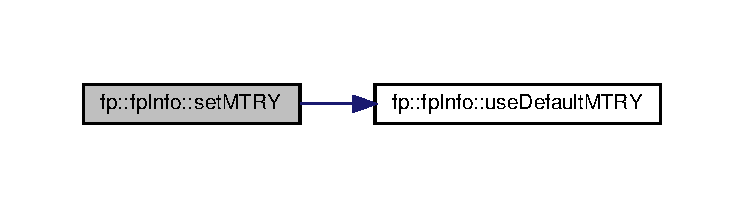
\includegraphics[width=350pt]{classfp_1_1fpInfo_a6b2a54fb9b3672e7b1bab3474a0ca33f_cgraph}
\end{center}
\end{figure}
\mbox{\Hypertarget{classfp_1_1fpInfo_a3598d1ab13bf05b53858b1ca8c44fa68}\label{classfp_1_1fpInfo_a3598d1ab13bf05b53858b1ca8c44fa68}} 
\index{fp\+::fp\+Info@{fp\+::fp\+Info}!set\+Num\+Classes@{set\+Num\+Classes}}
\index{set\+Num\+Classes@{set\+Num\+Classes}!fp\+::fp\+Info@{fp\+::fp\+Info}}
\subsubsection{\texorpdfstring{set\+Num\+Classes()}{setNumClasses()}}
{\footnotesize\ttfamily void fp\+::fp\+Info\+::set\+Num\+Classes (\begin{DoxyParamCaption}\item[{int}]{numC }\end{DoxyParamCaption})\hspace{0.3cm}{\ttfamily [inline]}}



Definition at line 73 of file fp\+Info.\+h.


\begin{DoxyCode}
73                                                \{
74                 \hyperlink{classfp_1_1fpInfo_a1c98a9ced12230f21003f78d742625a3}{numClasses} = numC;
75             \}
\end{DoxyCode}
\mbox{\Hypertarget{classfp_1_1fpInfo_a69ef99f2ec9ef74dd3787bc33ffb05d0}\label{classfp_1_1fpInfo_a69ef99f2ec9ef74dd3787bc33ffb05d0}} 
\index{fp\+::fp\+Info@{fp\+::fp\+Info}!set\+Num\+Features@{set\+Num\+Features}}
\index{set\+Num\+Features@{set\+Num\+Features}!fp\+::fp\+Info@{fp\+::fp\+Info}}
\subsubsection{\texorpdfstring{set\+Num\+Features()}{setNumFeatures()}}
{\footnotesize\ttfamily void fp\+::fp\+Info\+::set\+Num\+Features (\begin{DoxyParamCaption}\item[{int}]{numF }\end{DoxyParamCaption})\hspace{0.3cm}{\ttfamily [inline]}}



Definition at line 77 of file fp\+Info.\+h.


\begin{DoxyCode}
77                                                 \{
78                 \hyperlink{classfp_1_1fpInfo_a6ed8deabebae772fc213730cd29a2e61}{numFeatures} = numF;
79             \}
\end{DoxyCode}
\mbox{\Hypertarget{classfp_1_1fpInfo_ad17492e79df7bca55d98438fec2f004b}\label{classfp_1_1fpInfo_ad17492e79df7bca55d98438fec2f004b}} 
\index{fp\+::fp\+Info@{fp\+::fp\+Info}!set\+Num\+Observations@{set\+Num\+Observations}}
\index{set\+Num\+Observations@{set\+Num\+Observations}!fp\+::fp\+Info@{fp\+::fp\+Info}}
\subsubsection{\texorpdfstring{set\+Num\+Observations()}{setNumObservations()}}
{\footnotesize\ttfamily void fp\+::fp\+Info\+::set\+Num\+Observations (\begin{DoxyParamCaption}\item[{int}]{numO }\end{DoxyParamCaption})\hspace{0.3cm}{\ttfamily [inline]}}



Definition at line 81 of file fp\+Info.\+h.


\begin{DoxyCode}
81                                                     \{
82                 \hyperlink{classfp_1_1fpInfo_a1b35cd17d4ddb35e232246a6549d7a74}{numObservations} = numO;
83             \}
\end{DoxyCode}
\mbox{\Hypertarget{classfp_1_1fpInfo_ae4c749c466e983cb312cc08d38b2796e}\label{classfp_1_1fpInfo_ae4c749c466e983cb312cc08d38b2796e}} 
\index{fp\+::fp\+Info@{fp\+::fp\+Info}!set\+Parameter@{set\+Parameter}}
\index{set\+Parameter@{set\+Parameter}!fp\+::fp\+Info@{fp\+::fp\+Info}}
\subsubsection{\texorpdfstring{set\+Parameter()}{setParameter()}\hspace{0.1cm}{\footnotesize\ttfamily [1/3]}}
{\footnotesize\ttfamily void fp\+::fp\+Info\+::set\+Parameter (\begin{DoxyParamCaption}\item[{const std\+::string \&}]{parameter\+Name,  }\item[{const std\+::string \&}]{parameter\+Value }\end{DoxyParamCaption})}



Definition at line 13 of file fp\+Info.\+cpp.


\begin{DoxyCode}
13                                                                                             \{
14         \textcolor{keywordflow}{if}(parameterName == \textcolor{stringliteral}{"forestType"})\{
15             \hyperlink{classfp_1_1fpInfo_a3001fbf80d86022e53578d6adf133b90}{forestType} = parameterValue;
16         \}\textcolor{keywordflow}{else} \textcolor{keywordflow}{if}(parameterName == \textcolor{stringliteral}{"CSVFileName"})\{
17             \hyperlink{classfp_1_1fpInfo_aac01e5ddb27bc333e172a0422066af1c}{CSVFileName} = parameterValue;
18         \}\textcolor{keywordflow}{else}\{
19             \textcolor{keywordflow}{throw} std::runtime\_error(\textcolor{stringliteral}{"Unknown parameter type.(string)"});
20         \}
21     \}
\end{DoxyCode}
\mbox{\Hypertarget{classfp_1_1fpInfo_a8ef4332ee98a1724ffd8614c4f80af91}\label{classfp_1_1fpInfo_a8ef4332ee98a1724ffd8614c4f80af91}} 
\index{fp\+::fp\+Info@{fp\+::fp\+Info}!set\+Parameter@{set\+Parameter}}
\index{set\+Parameter@{set\+Parameter}!fp\+::fp\+Info@{fp\+::fp\+Info}}
\subsubsection{\texorpdfstring{set\+Parameter()}{setParameter()}\hspace{0.1cm}{\footnotesize\ttfamily [2/3]}}
{\footnotesize\ttfamily void fp\+::fp\+Info\+::set\+Parameter (\begin{DoxyParamCaption}\item[{const std\+::string \&}]{parameter\+Name,  }\item[{const double}]{parameter\+Value }\end{DoxyParamCaption})}



Definition at line 24 of file fp\+Info.\+cpp.


\begin{DoxyCode}
24                                                                                         \{
25         \textcolor{keywordflow}{if}(parameterName == \textcolor{stringliteral}{"numTreesInForest"})\{
26             \hyperlink{classfp_1_1fpInfo_a8dbd62dca5c972c29d29a69d90ca2632}{numTreesInForest} = (int)parameterValue;
27         \}\textcolor{keywordflow}{else} \textcolor{keywordflow}{if}(parameterName == \textcolor{stringliteral}{"minParent"})\{
28             \hyperlink{classfp_1_1fpInfo_a128fab7ba6da0fc76da00b48bb1bd7d5}{minParent} = (int)parameterValue;
29         \}\textcolor{keywordflow}{else} \textcolor{keywordflow}{if}(parameterName == \textcolor{stringliteral}{"numClasses"})\{
30             \hyperlink{classfp_1_1fpInfo_a1c98a9ced12230f21003f78d742625a3}{numClasses} = (int)parameterValue;
31         \}\textcolor{keywordflow}{else} \textcolor{keywordflow}{if}(parameterName == \textcolor{stringliteral}{"mtry"})\{
32             \hyperlink{classfp_1_1fpInfo_a62cccc1eb5641ebec2a6cc86cf03eedf}{mtry} = (int)parameterValue;
33         \}\textcolor{keywordflow}{else} \textcolor{keywordflow}{if}(parameterName == \textcolor{stringliteral}{"fractionOfFeaturesToTest"})\{
34             \hyperlink{classfp_1_1fpInfo_ab949cb97523283367e9b120fd78e3c3b}{fractionOfFeaturesToTest} = parameterValue;
35         \}\textcolor{keywordflow}{else} \textcolor{keywordflow}{if}(parameterName == \textcolor{stringliteral}{"columnWithY"})\{
36             \hyperlink{classfp_1_1fpInfo_ac29e135cd84cdef547b678e7ea37f92d}{columnWithY} = parameterValue;
37         \}\textcolor{keywordflow}{else} \{
38             \textcolor{keywordflow}{throw} std::runtime\_error(\textcolor{stringliteral}{"Unknown parameter type.(double)"});
39         \}
40     \}
\end{DoxyCode}
\mbox{\Hypertarget{classfp_1_1fpInfo_aa2dd574c5a3764c250f1ccb1b11de1e0}\label{classfp_1_1fpInfo_aa2dd574c5a3764c250f1ccb1b11de1e0}} 
\index{fp\+::fp\+Info@{fp\+::fp\+Info}!set\+Parameter@{set\+Parameter}}
\index{set\+Parameter@{set\+Parameter}!fp\+::fp\+Info@{fp\+::fp\+Info}}
\subsubsection{\texorpdfstring{set\+Parameter()}{setParameter()}\hspace{0.1cm}{\footnotesize\ttfamily [3/3]}}
{\footnotesize\ttfamily void fp\+::fp\+Info\+::set\+Parameter (\begin{DoxyParamCaption}\item[{const std\+::string \&}]{parameter\+Name,  }\item[{const int}]{parameter\+Value }\end{DoxyParamCaption})}



Definition at line 43 of file fp\+Info.\+cpp.


\begin{DoxyCode}
43                                                                                      \{
44         \textcolor{keywordflow}{if}(parameterName == \textcolor{stringliteral}{"numTreesInForest"})\{
45             \hyperlink{classfp_1_1fpInfo_a8dbd62dca5c972c29d29a69d90ca2632}{numTreesInForest} = parameterValue;
46         \}\textcolor{keywordflow}{else} \textcolor{keywordflow}{if}(parameterName == \textcolor{stringliteral}{"minParent"})\{
47             \hyperlink{classfp_1_1fpInfo_a128fab7ba6da0fc76da00b48bb1bd7d5}{minParent} = parameterValue;
48         \}\textcolor{keywordflow}{else} \textcolor{keywordflow}{if}(parameterName == \textcolor{stringliteral}{"numClasses"})\{
49             \hyperlink{classfp_1_1fpInfo_a1c98a9ced12230f21003f78d742625a3}{numClasses} = parameterValue;
50         \}\textcolor{keywordflow}{else} \textcolor{keywordflow}{if}(parameterName == \textcolor{stringliteral}{"mtry"})\{
51             \hyperlink{classfp_1_1fpInfo_a62cccc1eb5641ebec2a6cc86cf03eedf}{mtry} = parameterValue;
52         \}\textcolor{keywordflow}{else} \textcolor{keywordflow}{if}(parameterName == \textcolor{stringliteral}{"fractionOfFeaturesToTest"})\{
53             \hyperlink{classfp_1_1fpInfo_ab949cb97523283367e9b120fd78e3c3b}{fractionOfFeaturesToTest} = (double)parameterValue;
54         \}\textcolor{keywordflow}{else} \textcolor{keywordflow}{if}(parameterName == \textcolor{stringliteral}{"columnWithY"})\{
55             \hyperlink{classfp_1_1fpInfo_ac29e135cd84cdef547b678e7ea37f92d}{columnWithY} = parameterValue;
56         \}\textcolor{keywordflow}{else} \{
57             \textcolor{keywordflow}{throw} std::runtime\_error(\textcolor{stringliteral}{"Unknown parameter type.(int)"});
58         \}
59     \}
\end{DoxyCode}
\mbox{\Hypertarget{classfp_1_1fpInfo_a0a00d3d54cef667000249202a2d768bf}\label{classfp_1_1fpInfo_a0a00d3d54cef667000249202a2d768bf}} 
\index{fp\+::fp\+Info@{fp\+::fp\+Info}!use\+Default\+M\+T\+RY@{use\+Default\+M\+T\+RY}}
\index{use\+Default\+M\+T\+RY@{use\+Default\+M\+T\+RY}!fp\+::fp\+Info@{fp\+::fp\+Info}}
\subsubsection{\texorpdfstring{use\+Default\+M\+T\+R\+Y()}{useDefaultMTRY()}}
{\footnotesize\ttfamily bool fp\+::fp\+Info\+::use\+Default\+M\+T\+RY (\begin{DoxyParamCaption}{ }\end{DoxyParamCaption})\hspace{0.3cm}{\ttfamily [inline]}}



Definition at line 99 of file fp\+Info.\+h.


\begin{DoxyCode}
99                                         \{
100                 \textcolor{keywordflow}{return} \hyperlink{classfp_1_1fpInfo_ab949cb97523283367e9b120fd78e3c3b}{fractionOfFeaturesToTest} < 0;
101             \}
\end{DoxyCode}


\subsection{Member Data Documentation}
\mbox{\Hypertarget{classfp_1_1fpInfo_ac29e135cd84cdef547b678e7ea37f92d}\label{classfp_1_1fpInfo_ac29e135cd84cdef547b678e7ea37f92d}} 
\index{fp\+::fp\+Info@{fp\+::fp\+Info}!column\+WithY@{column\+WithY}}
\index{column\+WithY@{column\+WithY}!fp\+::fp\+Info@{fp\+::fp\+Info}}
\subsubsection{\texorpdfstring{column\+WithY}{columnWithY}}
{\footnotesize\ttfamily int fp\+::fp\+Info\+::column\+WithY = -\/1\hspace{0.3cm}{\ttfamily [protected]}}



Definition at line 20 of file fp\+Info.\+h.

\mbox{\Hypertarget{classfp_1_1fpInfo_aac01e5ddb27bc333e172a0422066af1c}\label{classfp_1_1fpInfo_aac01e5ddb27bc333e172a0422066af1c}} 
\index{fp\+::fp\+Info@{fp\+::fp\+Info}!C\+S\+V\+File\+Name@{C\+S\+V\+File\+Name}}
\index{C\+S\+V\+File\+Name@{C\+S\+V\+File\+Name}!fp\+::fp\+Info@{fp\+::fp\+Info}}
\subsubsection{\texorpdfstring{C\+S\+V\+File\+Name}{CSVFileName}}
{\footnotesize\ttfamily std\+::string fp\+::fp\+Info\+::\+C\+S\+V\+File\+Name\hspace{0.3cm}{\ttfamily [protected]}}



Definition at line 29 of file fp\+Info.\+h.

\mbox{\Hypertarget{classfp_1_1fpInfo_a3001fbf80d86022e53578d6adf133b90}\label{classfp_1_1fpInfo_a3001fbf80d86022e53578d6adf133b90}} 
\index{fp\+::fp\+Info@{fp\+::fp\+Info}!forest\+Type@{forest\+Type}}
\index{forest\+Type@{forest\+Type}!fp\+::fp\+Info@{fp\+::fp\+Info}}
\subsubsection{\texorpdfstring{forest\+Type}{forestType}}
{\footnotesize\ttfamily std\+::string fp\+::fp\+Info\+::forest\+Type\hspace{0.3cm}{\ttfamily [protected]}}



Definition at line 28 of file fp\+Info.\+h.

\mbox{\Hypertarget{classfp_1_1fpInfo_ab949cb97523283367e9b120fd78e3c3b}\label{classfp_1_1fpInfo_ab949cb97523283367e9b120fd78e3c3b}} 
\index{fp\+::fp\+Info@{fp\+::fp\+Info}!fraction\+Of\+Features\+To\+Test@{fraction\+Of\+Features\+To\+Test}}
\index{fraction\+Of\+Features\+To\+Test@{fraction\+Of\+Features\+To\+Test}!fp\+::fp\+Info@{fp\+::fp\+Info}}
\subsubsection{\texorpdfstring{fraction\+Of\+Features\+To\+Test}{fractionOfFeaturesToTest}}
{\footnotesize\ttfamily double fp\+::fp\+Info\+::fraction\+Of\+Features\+To\+Test = -\/1.\+0\hspace{0.3cm}{\ttfamily [protected]}}



Definition at line 26 of file fp\+Info.\+h.

\mbox{\Hypertarget{classfp_1_1fpInfo_a95c744fa049788dd61fa0fccdec4565d}\label{classfp_1_1fpInfo_a95c744fa049788dd61fa0fccdec4565d}} 
\index{fp\+::fp\+Info@{fp\+::fp\+Info}!max\+Depth@{max\+Depth}}
\index{max\+Depth@{max\+Depth}!fp\+::fp\+Info@{fp\+::fp\+Info}}
\subsubsection{\texorpdfstring{max\+Depth}{maxDepth}}
{\footnotesize\ttfamily int fp\+::fp\+Info\+::max\+Depth\hspace{0.3cm}{\ttfamily [protected]}}



Definition at line 23 of file fp\+Info.\+h.

\mbox{\Hypertarget{classfp_1_1fpInfo_a128fab7ba6da0fc76da00b48bb1bd7d5}\label{classfp_1_1fpInfo_a128fab7ba6da0fc76da00b48bb1bd7d5}} 
\index{fp\+::fp\+Info@{fp\+::fp\+Info}!min\+Parent@{min\+Parent}}
\index{min\+Parent@{min\+Parent}!fp\+::fp\+Info@{fp\+::fp\+Info}}
\subsubsection{\texorpdfstring{min\+Parent}{minParent}}
{\footnotesize\ttfamily int fp\+::fp\+Info\+::min\+Parent = 1\hspace{0.3cm}{\ttfamily [protected]}}



Definition at line 15 of file fp\+Info.\+h.

\mbox{\Hypertarget{classfp_1_1fpInfo_a62cccc1eb5641ebec2a6cc86cf03eedf}\label{classfp_1_1fpInfo_a62cccc1eb5641ebec2a6cc86cf03eedf}} 
\index{fp\+::fp\+Info@{fp\+::fp\+Info}!mtry@{mtry}}
\index{mtry@{mtry}!fp\+::fp\+Info@{fp\+::fp\+Info}}
\subsubsection{\texorpdfstring{mtry}{mtry}}
{\footnotesize\ttfamily int fp\+::fp\+Info\+::mtry = -\/1\hspace{0.3cm}{\ttfamily [protected]}}



Definition at line 19 of file fp\+Info.\+h.

\mbox{\Hypertarget{classfp_1_1fpInfo_a9404de3ad49dc78e3d5c8e3ef8b04fba}\label{classfp_1_1fpInfo_a9404de3ad49dc78e3d5c8e3ef8b04fba}} 
\index{fp\+::fp\+Info@{fp\+::fp\+Info}!number\+Of\+Nodes@{number\+Of\+Nodes}}
\index{number\+Of\+Nodes@{number\+Of\+Nodes}!fp\+::fp\+Info@{fp\+::fp\+Info}}
\subsubsection{\texorpdfstring{number\+Of\+Nodes}{numberOfNodes}}
{\footnotesize\ttfamily int fp\+::fp\+Info\+::number\+Of\+Nodes\hspace{0.3cm}{\ttfamily [protected]}}



Definition at line 22 of file fp\+Info.\+h.

\mbox{\Hypertarget{classfp_1_1fpInfo_a1c98a9ced12230f21003f78d742625a3}\label{classfp_1_1fpInfo_a1c98a9ced12230f21003f78d742625a3}} 
\index{fp\+::fp\+Info@{fp\+::fp\+Info}!num\+Classes@{num\+Classes}}
\index{num\+Classes@{num\+Classes}!fp\+::fp\+Info@{fp\+::fp\+Info}}
\subsubsection{\texorpdfstring{num\+Classes}{numClasses}}
{\footnotesize\ttfamily int fp\+::fp\+Info\+::num\+Classes = -\/1\hspace{0.3cm}{\ttfamily [protected]}}



Definition at line 16 of file fp\+Info.\+h.

\mbox{\Hypertarget{classfp_1_1fpInfo_a6ed8deabebae772fc213730cd29a2e61}\label{classfp_1_1fpInfo_a6ed8deabebae772fc213730cd29a2e61}} 
\index{fp\+::fp\+Info@{fp\+::fp\+Info}!num\+Features@{num\+Features}}
\index{num\+Features@{num\+Features}!fp\+::fp\+Info@{fp\+::fp\+Info}}
\subsubsection{\texorpdfstring{num\+Features}{numFeatures}}
{\footnotesize\ttfamily int fp\+::fp\+Info\+::num\+Features = -\/1\hspace{0.3cm}{\ttfamily [protected]}}



Definition at line 18 of file fp\+Info.\+h.

\mbox{\Hypertarget{classfp_1_1fpInfo_a1b35cd17d4ddb35e232246a6549d7a74}\label{classfp_1_1fpInfo_a1b35cd17d4ddb35e232246a6549d7a74}} 
\index{fp\+::fp\+Info@{fp\+::fp\+Info}!num\+Observations@{num\+Observations}}
\index{num\+Observations@{num\+Observations}!fp\+::fp\+Info@{fp\+::fp\+Info}}
\subsubsection{\texorpdfstring{num\+Observations}{numObservations}}
{\footnotesize\ttfamily int fp\+::fp\+Info\+::num\+Observations = -\/1\hspace{0.3cm}{\ttfamily [protected]}}



Definition at line 17 of file fp\+Info.\+h.

\mbox{\Hypertarget{classfp_1_1fpInfo_a8dbd62dca5c972c29d29a69d90ca2632}\label{classfp_1_1fpInfo_a8dbd62dca5c972c29d29a69d90ca2632}} 
\index{fp\+::fp\+Info@{fp\+::fp\+Info}!num\+Trees\+In\+Forest@{num\+Trees\+In\+Forest}}
\index{num\+Trees\+In\+Forest@{num\+Trees\+In\+Forest}!fp\+::fp\+Info@{fp\+::fp\+Info}}
\subsubsection{\texorpdfstring{num\+Trees\+In\+Forest}{numTreesInForest}}
{\footnotesize\ttfamily int fp\+::fp\+Info\+::num\+Trees\+In\+Forest\hspace{0.3cm}{\ttfamily [protected]}}



Definition at line 14 of file fp\+Info.\+h.

\mbox{\Hypertarget{classfp_1_1fpInfo_a13afa17097728f059e8525ea382b71cd}\label{classfp_1_1fpInfo_a13afa17097728f059e8525ea382b71cd}} 
\index{fp\+::fp\+Info@{fp\+::fp\+Info}!sum\+Leaf\+Node\+Depths@{sum\+Leaf\+Node\+Depths}}
\index{sum\+Leaf\+Node\+Depths@{sum\+Leaf\+Node\+Depths}!fp\+::fp\+Info@{fp\+::fp\+Info}}
\subsubsection{\texorpdfstring{sum\+Leaf\+Node\+Depths}{sumLeafNodeDepths}}
{\footnotesize\ttfamily int fp\+::fp\+Info\+::sum\+Leaf\+Node\+Depths\hspace{0.3cm}{\ttfamily [protected]}}



Definition at line 24 of file fp\+Info.\+h.



The documentation for this class was generated from the following files\+:\begin{DoxyCompactItemize}
\item 
src/fp\+Singleton/\hyperlink{fpInfo_8h}{fp\+Info.\+h}\item 
src/fp\+Singleton/\hyperlink{fpInfo_8cpp}{fp\+Info.\+cpp}\end{DoxyCompactItemize}

\hypertarget{classfp_1_1fpRerFBase}{}\section{fp\+:\+:fp\+Rer\+F\+Base$<$ T $>$ Class Template Reference}
\label{classfp_1_1fpRerFBase}\index{fp\+::fp\+Rer\+F\+Base$<$ T $>$@{fp\+::fp\+Rer\+F\+Base$<$ T $>$}}


{\ttfamily \#include $<$fp\+Rer\+F\+Base.\+h$>$}



Inheritance diagram for fp\+:\+:fp\+Rer\+F\+Base$<$ T $>$\+:
\nopagebreak
\begin{figure}[H]
\begin{center}
\leavevmode
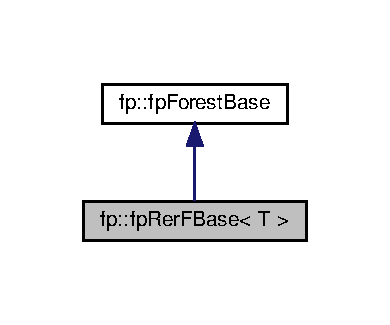
\includegraphics[width=187pt]{classfp_1_1fpRerFBase__inherit__graph}
\end{center}
\end{figure}


Collaboration diagram for fp\+:\+:fp\+Rer\+F\+Base$<$ T $>$\+:
\nopagebreak
\begin{figure}[H]
\begin{center}
\leavevmode
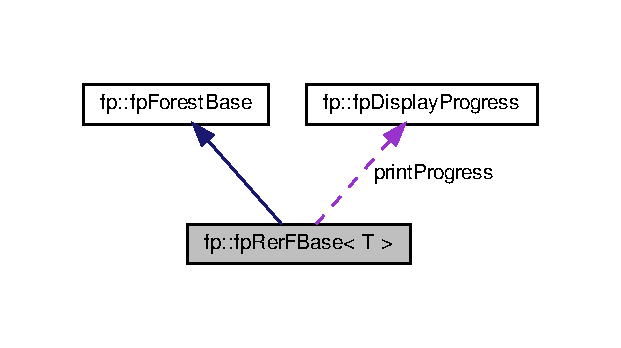
\includegraphics[width=298pt]{classfp_1_1fpRerFBase__coll__graph}
\end{center}
\end{figure}
\subsection*{Public Member Functions}
\begin{DoxyCompactItemize}
\item 
\hyperlink{classfp_1_1fpRerFBase_a3c48a1913e8affa4a4a3b2373207dbd4}{fp\+Rer\+F\+Base} ()
\item 
void \hyperlink{classfp_1_1fpRerFBase_ade8132388aa51aca41c80986003070e4}{print\+Forest\+Type} ()
\item 
void \hyperlink{classfp_1_1fpRerFBase_a4aa9be48cadab132857ea9d9da18fe8a}{change\+Forest\+Size} ()
\item 
void \hyperlink{classfp_1_1fpRerFBase_a5faf8bb9221d903880e0bd6660ea4d0d}{grow\+Trees} ()
\item 
void \hyperlink{classfp_1_1fpRerFBase_ae458c0b2743862b693ded729bf00b218}{check\+Parameters} ()
\item 
void \hyperlink{classfp_1_1fpRerFBase_ad9983abf38c0cb799ed490129508d42e}{tree\+Stats} ()
\item 
void \hyperlink{classfp_1_1fpRerFBase_af55265f8a05b0dd1aab826738cefd628}{print\+Tree0} ()
\item 
void \hyperlink{classfp_1_1fpRerFBase_a0205440403a691b7644a6af0ef796d7a}{grow\+Forest} ()
\item 
int \hyperlink{classfp_1_1fpRerFBase_a73ece66e774ad5f1a450f1422626947f}{predict\+Class} (int observation\+Number)
\item 
float \hyperlink{classfp_1_1fpRerFBase_a0ea48ea24a8213e49e18b6f24ab45508}{test\+Forest} ()
\end{DoxyCompactItemize}
\subsection*{Public Attributes}
\begin{DoxyCompactItemize}
\item 
\hyperlink{classfp_1_1fpDisplayProgress}{fp\+Display\+Progress} \hyperlink{classfp_1_1fpRerFBase_a539e79a960846182fc49420d79896ba1}{print\+Progress}
\end{DoxyCompactItemize}
\subsection*{Protected Attributes}
\begin{DoxyCompactItemize}
\item 
std\+::vector$<$ \hyperlink{classfp_1_1rerfTree}{rerf\+Tree}$<$ T $>$ $>$ \hyperlink{classfp_1_1fpRerFBase_a6c2f12312e64e5234fc53741f1bfbe96}{trees}
\end{DoxyCompactItemize}


\subsection{Detailed Description}
\subsubsection*{template$<$typename T$>$\newline
class fp\+::fp\+Rer\+F\+Base$<$ T $>$}



Definition at line 16 of file fp\+Rer\+F\+Base.\+h.



\subsection{Constructor \& Destructor Documentation}
\mbox{\Hypertarget{classfp_1_1fpRerFBase_a3c48a1913e8affa4a4a3b2373207dbd4}\label{classfp_1_1fpRerFBase_a3c48a1913e8affa4a4a3b2373207dbd4}} 
\index{fp\+::fp\+Rer\+F\+Base@{fp\+::fp\+Rer\+F\+Base}!fp\+Rer\+F\+Base@{fp\+Rer\+F\+Base}}
\index{fp\+Rer\+F\+Base@{fp\+Rer\+F\+Base}!fp\+::fp\+Rer\+F\+Base@{fp\+::fp\+Rer\+F\+Base}}
\subsubsection{\texorpdfstring{fp\+Rer\+F\+Base()}{fpRerFBase()}}
{\footnotesize\ttfamily template$<$typename T $>$ \\
\hyperlink{classfp_1_1fpRerFBase}{fp\+::fp\+Rer\+F\+Base}$<$ T $>$\+::\hyperlink{classfp_1_1fpRerFBase}{fp\+Rer\+F\+Base} (\begin{DoxyParamCaption}{ }\end{DoxyParamCaption})\hspace{0.3cm}{\ttfamily [inline]}}



Definition at line 23 of file fp\+Rer\+F\+Base.\+h.


\begin{DoxyCode}
23                         \{
24                 std::srand(\textcolor{keywordtype}{unsigned}(std::time(0)));
25             \}
\end{DoxyCode}


\subsection{Member Function Documentation}
\mbox{\Hypertarget{classfp_1_1fpRerFBase_a4aa9be48cadab132857ea9d9da18fe8a}\label{classfp_1_1fpRerFBase_a4aa9be48cadab132857ea9d9da18fe8a}} 
\index{fp\+::fp\+Rer\+F\+Base@{fp\+::fp\+Rer\+F\+Base}!change\+Forest\+Size@{change\+Forest\+Size}}
\index{change\+Forest\+Size@{change\+Forest\+Size}!fp\+::fp\+Rer\+F\+Base@{fp\+::fp\+Rer\+F\+Base}}
\subsubsection{\texorpdfstring{change\+Forest\+Size()}{changeForestSize()}}
{\footnotesize\ttfamily template$<$typename T $>$ \\
void \hyperlink{classfp_1_1fpRerFBase}{fp\+::fp\+Rer\+F\+Base}$<$ T $>$\+::change\+Forest\+Size (\begin{DoxyParamCaption}{ }\end{DoxyParamCaption})\hspace{0.3cm}{\ttfamily [inline]}}



Definition at line 32 of file fp\+Rer\+F\+Base.\+h.


\begin{DoxyCode}
32                                    \{
33                 \hyperlink{classfp_1_1fpRerFBase_a6c2f12312e64e5234fc53741f1bfbe96}{trees}.resize(\hyperlink{classfp_1_1fpSingleton_a8bdae77b68521003e3fc630edec2e240}{fpSingleton::getSingleton}().returnNumTrees());
34             \}
\end{DoxyCode}
Here is the call graph for this function\+:
\nopagebreak
\begin{figure}[H]
\begin{center}
\leavevmode
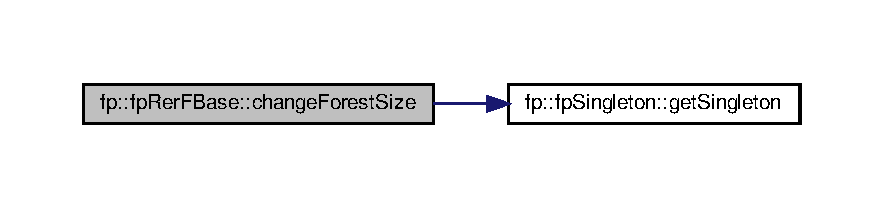
\includegraphics[width=350pt]{classfp_1_1fpRerFBase_a4aa9be48cadab132857ea9d9da18fe8a_cgraph}
\end{center}
\end{figure}
\mbox{\Hypertarget{classfp_1_1fpRerFBase_ae458c0b2743862b693ded729bf00b218}\label{classfp_1_1fpRerFBase_ae458c0b2743862b693ded729bf00b218}} 
\index{fp\+::fp\+Rer\+F\+Base@{fp\+::fp\+Rer\+F\+Base}!check\+Parameters@{check\+Parameters}}
\index{check\+Parameters@{check\+Parameters}!fp\+::fp\+Rer\+F\+Base@{fp\+::fp\+Rer\+F\+Base}}
\subsubsection{\texorpdfstring{check\+Parameters()}{checkParameters()}}
{\footnotesize\ttfamily template$<$typename T $>$ \\
void \hyperlink{classfp_1_1fpRerFBase}{fp\+::fp\+Rer\+F\+Base}$<$ T $>$\+::check\+Parameters (\begin{DoxyParamCaption}{ }\end{DoxyParamCaption})\hspace{0.3cm}{\ttfamily [inline]}}



Definition at line 45 of file fp\+Rer\+F\+Base.\+h.


\begin{DoxyCode}
45                                          \{
46                 \textcolor{comment}{//TODO: check parameters to make sure they make sense for this forest type.}
47                 ;
48             \}
\end{DoxyCode}
\mbox{\Hypertarget{classfp_1_1fpRerFBase_a0205440403a691b7644a6af0ef796d7a}\label{classfp_1_1fpRerFBase_a0205440403a691b7644a6af0ef796d7a}} 
\index{fp\+::fp\+Rer\+F\+Base@{fp\+::fp\+Rer\+F\+Base}!grow\+Forest@{grow\+Forest}}
\index{grow\+Forest@{grow\+Forest}!fp\+::fp\+Rer\+F\+Base@{fp\+::fp\+Rer\+F\+Base}}
\subsubsection{\texorpdfstring{grow\+Forest()}{growForest()}}
{\footnotesize\ttfamily template$<$typename T $>$ \\
void \hyperlink{classfp_1_1fpRerFBase}{fp\+::fp\+Rer\+F\+Base}$<$ T $>$\+::grow\+Forest (\begin{DoxyParamCaption}{ }\end{DoxyParamCaption})\hspace{0.3cm}{\ttfamily [inline]}, {\ttfamily [virtual]}}



Implements \hyperlink{classfp_1_1fpForestBase_a05b1d924a559536083ee7a8cf3ea542d}{fp\+::fp\+Forest\+Base}.



Definition at line 73 of file fp\+Rer\+F\+Base.\+h.


\begin{DoxyCode}
73                              \{
74                 \textcolor{comment}{//  checkParameters();}
75                 \hyperlink{classfp_1_1fpRerFBase_a4aa9be48cadab132857ea9d9da18fe8a}{changeForestSize}();
76                 \hyperlink{classfp_1_1fpRerFBase_a5faf8bb9221d903880e0bd6660ea4d0d}{growTrees}();
77                 \hyperlink{classfp_1_1fpRerFBase_ad9983abf38c0cb799ed490129508d42e}{treeStats}();
78             \}
\end{DoxyCode}
Here is the call graph for this function\+:
\nopagebreak
\begin{figure}[H]
\begin{center}
\leavevmode
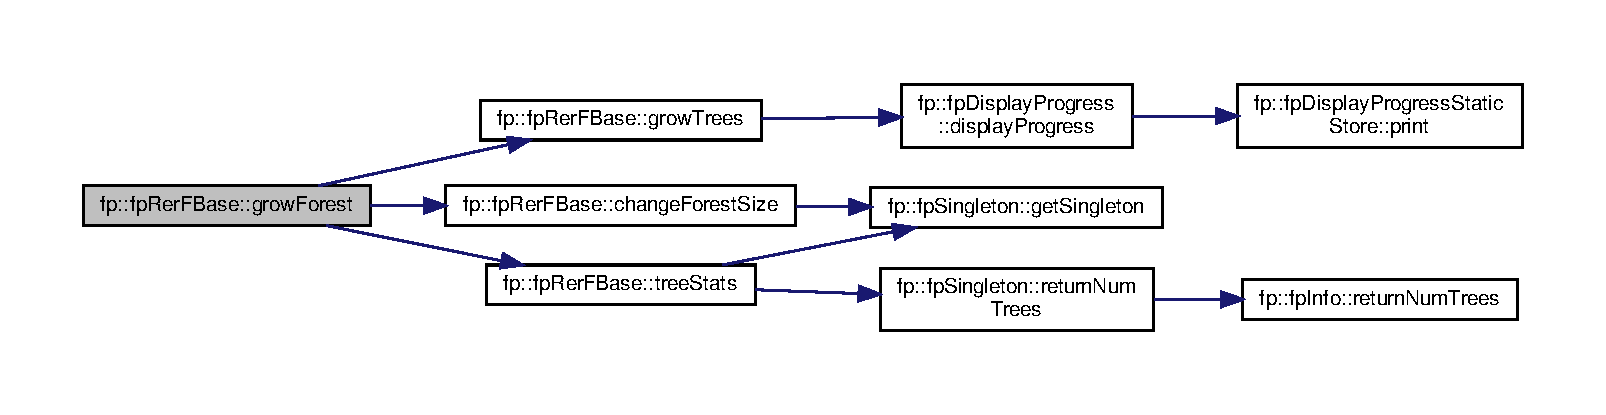
\includegraphics[width=350pt]{classfp_1_1fpRerFBase_a0205440403a691b7644a6af0ef796d7a_cgraph}
\end{center}
\end{figure}
\mbox{\Hypertarget{classfp_1_1fpRerFBase_a5faf8bb9221d903880e0bd6660ea4d0d}\label{classfp_1_1fpRerFBase_a5faf8bb9221d903880e0bd6660ea4d0d}} 
\index{fp\+::fp\+Rer\+F\+Base@{fp\+::fp\+Rer\+F\+Base}!grow\+Trees@{grow\+Trees}}
\index{grow\+Trees@{grow\+Trees}!fp\+::fp\+Rer\+F\+Base@{fp\+::fp\+Rer\+F\+Base}}
\subsubsection{\texorpdfstring{grow\+Trees()}{growTrees()}}
{\footnotesize\ttfamily template$<$typename T $>$ \\
void \hyperlink{classfp_1_1fpRerFBase}{fp\+::fp\+Rer\+F\+Base}$<$ T $>$\+::grow\+Trees (\begin{DoxyParamCaption}{ }\end{DoxyParamCaption})\hspace{0.3cm}{\ttfamily [inline]}}



Definition at line 36 of file fp\+Rer\+F\+Base.\+h.


\begin{DoxyCode}
36                             \{
37 
38                 \textcolor{keywordflow}{for}(\textcolor{keywordtype}{unsigned} \textcolor{keywordtype}{int} i = 0; i < \hyperlink{classfp_1_1fpRerFBase_a6c2f12312e64e5234fc53741f1bfbe96}{trees}.size(); ++i)\{
39                     \hyperlink{classfp_1_1fpRerFBase_a539e79a960846182fc49420d79896ba1}{printProgress}.\hyperlink{classfp_1_1fpDisplayProgress_adf5b2e390618d63eccb6de3b00eb857b}{displayProgress}(i);
40                     \hyperlink{classfp_1_1fpRerFBase_a6c2f12312e64e5234fc53741f1bfbe96}{trees}[i].growTree();
41                 \}
42                 std::cout << \textcolor{stringliteral}{"\(\backslash\)n"}<< std::flush;
43             \}
\end{DoxyCode}
Here is the call graph for this function\+:
\nopagebreak
\begin{figure}[H]
\begin{center}
\leavevmode
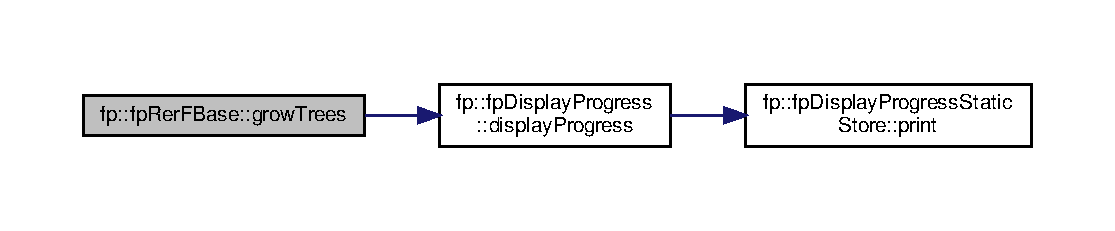
\includegraphics[width=350pt]{classfp_1_1fpRerFBase_a5faf8bb9221d903880e0bd6660ea4d0d_cgraph}
\end{center}
\end{figure}
\mbox{\Hypertarget{classfp_1_1fpRerFBase_a73ece66e774ad5f1a450f1422626947f}\label{classfp_1_1fpRerFBase_a73ece66e774ad5f1a450f1422626947f}} 
\index{fp\+::fp\+Rer\+F\+Base@{fp\+::fp\+Rer\+F\+Base}!predict\+Class@{predict\+Class}}
\index{predict\+Class@{predict\+Class}!fp\+::fp\+Rer\+F\+Base@{fp\+::fp\+Rer\+F\+Base}}
\subsubsection{\texorpdfstring{predict\+Class()}{predictClass()}}
{\footnotesize\ttfamily template$<$typename T $>$ \\
int \hyperlink{classfp_1_1fpRerFBase}{fp\+::fp\+Rer\+F\+Base}$<$ T $>$\+::predict\+Class (\begin{DoxyParamCaption}\item[{int}]{observation\+Number }\end{DoxyParamCaption})\hspace{0.3cm}{\ttfamily [inline]}}



Definition at line 80 of file fp\+Rer\+F\+Base.\+h.


\begin{DoxyCode}
80                                                           \{
81                 std::vector<int> classTally(\hyperlink{classfp_1_1fpSingleton_a8bdae77b68521003e3fc630edec2e240}{fpSingleton::getSingleton}().
      returnNumClasses(),0);
82                 \textcolor{keywordflow}{for}(\textcolor{keywordtype}{int} i = 0; i < \hyperlink{classfp_1_1fpSingleton_a8bdae77b68521003e3fc630edec2e240}{fpSingleton::getSingleton}().
      \hyperlink{classfp_1_1fpSingleton_a8be36616345b6b77ce4c60b99cc2b91c}{returnNumTrees}(); ++i)\{
83                     ++classTally[\hyperlink{classfp_1_1fpRerFBase_a6c2f12312e64e5234fc53741f1bfbe96}{trees}[i].predictObservation(observationNumber)];
84                 \}
85                 \textcolor{keywordtype}{int} bestClass = 0;
86                 \textcolor{keywordflow}{for}(\textcolor{keywordtype}{int} j = 1; j < \hyperlink{classfp_1_1fpSingleton_a8bdae77b68521003e3fc630edec2e240}{fpSingleton::getSingleton}().
      \hyperlink{classfp_1_1fpSingleton_a5602580110329a6b25602b1789e4e2c2}{returnNumClasses}(); ++j)\{
87                     \textcolor{keywordflow}{if}(classTally[bestClass] < classTally[j])\{
88                         bestClass = j;
89                     \}
90                 \}
91                 \textcolor{keywordflow}{return} bestClass;
92             \}
\end{DoxyCode}
Here is the call graph for this function\+:
\nopagebreak
\begin{figure}[H]
\begin{center}
\leavevmode
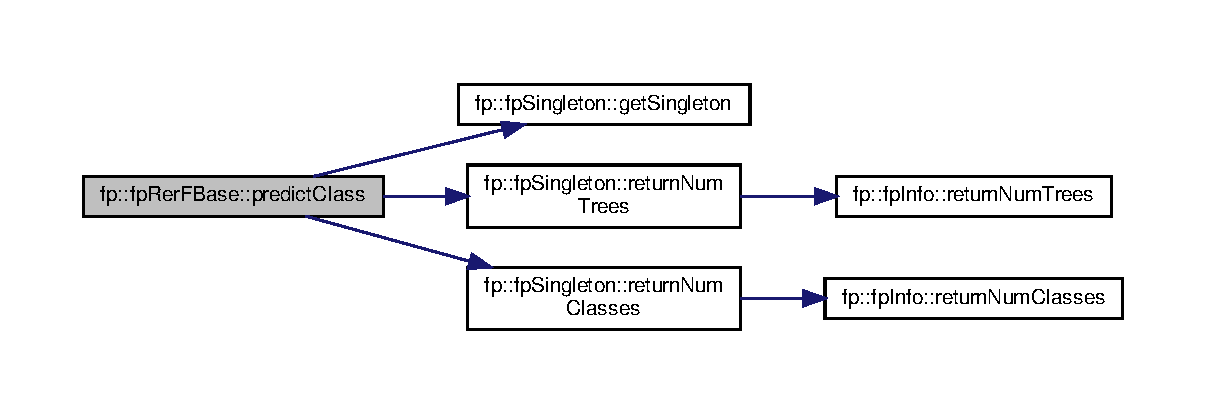
\includegraphics[width=350pt]{classfp_1_1fpRerFBase_a73ece66e774ad5f1a450f1422626947f_cgraph}
\end{center}
\end{figure}
\mbox{\Hypertarget{classfp_1_1fpRerFBase_ade8132388aa51aca41c80986003070e4}\label{classfp_1_1fpRerFBase_ade8132388aa51aca41c80986003070e4}} 
\index{fp\+::fp\+Rer\+F\+Base@{fp\+::fp\+Rer\+F\+Base}!print\+Forest\+Type@{print\+Forest\+Type}}
\index{print\+Forest\+Type@{print\+Forest\+Type}!fp\+::fp\+Rer\+F\+Base@{fp\+::fp\+Rer\+F\+Base}}
\subsubsection{\texorpdfstring{print\+Forest\+Type()}{printForestType()}}
{\footnotesize\ttfamily template$<$typename T $>$ \\
void \hyperlink{classfp_1_1fpRerFBase}{fp\+::fp\+Rer\+F\+Base}$<$ T $>$\+::print\+Forest\+Type (\begin{DoxyParamCaption}{ }\end{DoxyParamCaption})\hspace{0.3cm}{\ttfamily [inline]}, {\ttfamily [virtual]}}



Implements \hyperlink{classfp_1_1fpForestBase_a5e200f603cca94bb5d9f357489f07e97}{fp\+::fp\+Forest\+Base}.



Definition at line 28 of file fp\+Rer\+F\+Base.\+h.


\begin{DoxyCode}
28                                   \{
29                 std::cout << \textcolor{stringliteral}{"This is a rerf forest.\(\backslash\)n"};
30             \}
\end{DoxyCode}
\mbox{\Hypertarget{classfp_1_1fpRerFBase_af55265f8a05b0dd1aab826738cefd628}\label{classfp_1_1fpRerFBase_af55265f8a05b0dd1aab826738cefd628}} 
\index{fp\+::fp\+Rer\+F\+Base@{fp\+::fp\+Rer\+F\+Base}!print\+Tree0@{print\+Tree0}}
\index{print\+Tree0@{print\+Tree0}!fp\+::fp\+Rer\+F\+Base@{fp\+::fp\+Rer\+F\+Base}}
\subsubsection{\texorpdfstring{print\+Tree0()}{printTree0()}}
{\footnotesize\ttfamily template$<$typename T $>$ \\
void \hyperlink{classfp_1_1fpRerFBase}{fp\+::fp\+Rer\+F\+Base}$<$ T $>$\+::print\+Tree0 (\begin{DoxyParamCaption}{ }\end{DoxyParamCaption})\hspace{0.3cm}{\ttfamily [inline]}}



Definition at line 69 of file fp\+Rer\+F\+Base.\+h.


\begin{DoxyCode}
69                              \{
70                 \hyperlink{classfp_1_1fpRerFBase_a6c2f12312e64e5234fc53741f1bfbe96}{trees}[0].printTree();
71             \}
\end{DoxyCode}
\mbox{\Hypertarget{classfp_1_1fpRerFBase_a0ea48ea24a8213e49e18b6f24ab45508}\label{classfp_1_1fpRerFBase_a0ea48ea24a8213e49e18b6f24ab45508}} 
\index{fp\+::fp\+Rer\+F\+Base@{fp\+::fp\+Rer\+F\+Base}!test\+Forest@{test\+Forest}}
\index{test\+Forest@{test\+Forest}!fp\+::fp\+Rer\+F\+Base@{fp\+::fp\+Rer\+F\+Base}}
\subsubsection{\texorpdfstring{test\+Forest()}{testForest()}}
{\footnotesize\ttfamily template$<$typename T $>$ \\
float \hyperlink{classfp_1_1fpRerFBase}{fp\+::fp\+Rer\+F\+Base}$<$ T $>$\+::test\+Forest (\begin{DoxyParamCaption}{ }\end{DoxyParamCaption})\hspace{0.3cm}{\ttfamily [inline]}, {\ttfamily [virtual]}}



Implements \hyperlink{classfp_1_1fpForestBase_af7becba028a198f650841b718d16ed16}{fp\+::fp\+Forest\+Base}.



Definition at line 95 of file fp\+Rer\+F\+Base.\+h.


\begin{DoxyCode}
95                               \{
96                 \textcolor{keywordtype}{float} numTried = 0;
97                 \textcolor{keywordtype}{float} numWrong = 0;
98 
99                 \textcolor{keywordflow}{for} (\textcolor{keywordtype}{int} i = 0; i <\hyperlink{classfp_1_1fpSingleton_a8bdae77b68521003e3fc630edec2e240}{fpSingleton::getSingleton}().
      \hyperlink{classfp_1_1fpSingleton_ae0a2963feb07b809b8740218f1048b67}{returnNumObservations}();i++)\{
100                     ++numTried;
101                     \textcolor{keywordtype}{int} predClass = \hyperlink{classfp_1_1fpRerFBase_a73ece66e774ad5f1a450f1422626947f}{predictClass}(i);
102 
103                     \textcolor{keywordflow}{if}(predClass != \hyperlink{classfp_1_1fpSingleton_a8bdae77b68521003e3fc630edec2e240}{fpSingleton::getSingleton}().returnTestLabel(i)
      )\{
104                         ++numWrong;
105                     \}
106                 \}
107                 std::cout << \textcolor{stringliteral}{"\(\backslash\)nnumWrong= "} << numWrong << \textcolor{stringliteral}{"\(\backslash\)n"};
108 
109                 \textcolor{keywordflow}{return} numWrong/numTried;
110             \}
\end{DoxyCode}
Here is the call graph for this function\+:
\nopagebreak
\begin{figure}[H]
\begin{center}
\leavevmode
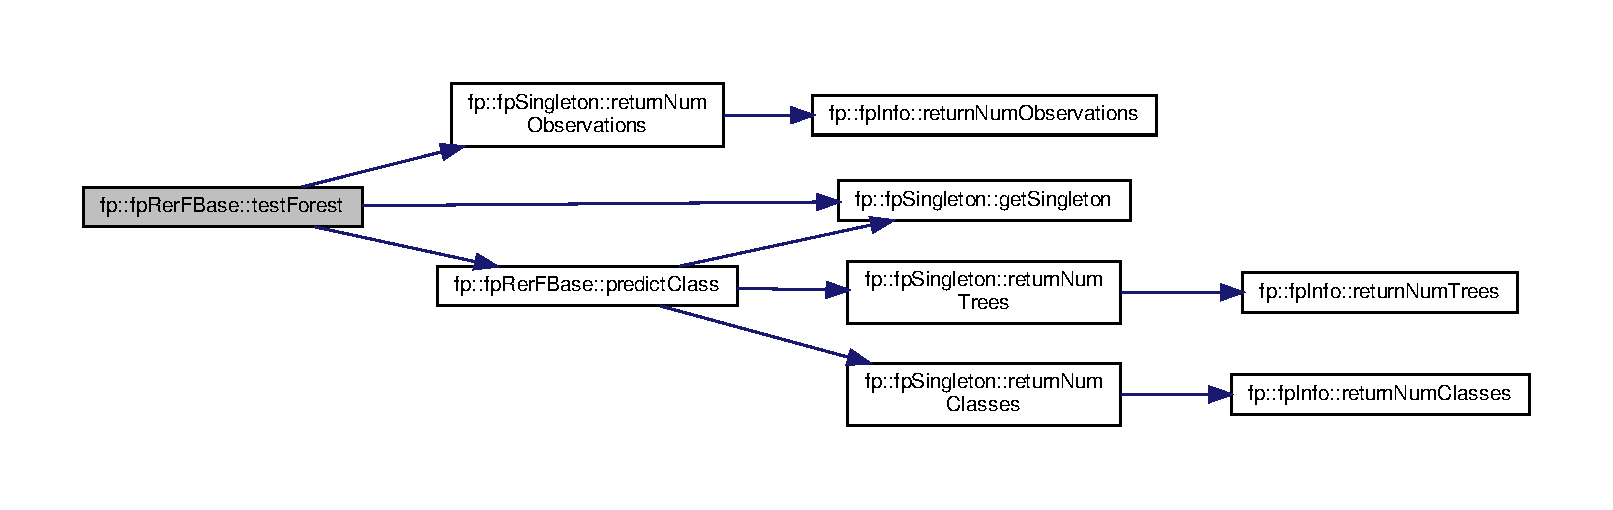
\includegraphics[width=350pt]{classfp_1_1fpRerFBase_a0ea48ea24a8213e49e18b6f24ab45508_cgraph}
\end{center}
\end{figure}
\mbox{\Hypertarget{classfp_1_1fpRerFBase_ad9983abf38c0cb799ed490129508d42e}\label{classfp_1_1fpRerFBase_ad9983abf38c0cb799ed490129508d42e}} 
\index{fp\+::fp\+Rer\+F\+Base@{fp\+::fp\+Rer\+F\+Base}!tree\+Stats@{tree\+Stats}}
\index{tree\+Stats@{tree\+Stats}!fp\+::fp\+Rer\+F\+Base@{fp\+::fp\+Rer\+F\+Base}}
\subsubsection{\texorpdfstring{tree\+Stats()}{treeStats()}}
{\footnotesize\ttfamily template$<$typename T $>$ \\
void \hyperlink{classfp_1_1fpRerFBase}{fp\+::fp\+Rer\+F\+Base}$<$ T $>$\+::tree\+Stats (\begin{DoxyParamCaption}{ }\end{DoxyParamCaption})\hspace{0.3cm}{\ttfamily [inline]}}



Definition at line 50 of file fp\+Rer\+F\+Base.\+h.


\begin{DoxyCode}
50                             \{
51                 \textcolor{keywordtype}{int} maxDepth=0;
52                 \textcolor{keywordtype}{int} totalLeafNodes=0;
53                 \textcolor{keywordtype}{int} totalLeafDepth=0;
54 
55                 \textcolor{keywordtype}{int} tempMaxDepth;
56                 \textcolor{keywordflow}{for}(\textcolor{keywordtype}{int} i = 0; i < \hyperlink{classfp_1_1fpSingleton_a8bdae77b68521003e3fc630edec2e240}{fpSingleton::getSingleton}().
      \hyperlink{classfp_1_1fpSingleton_a8be36616345b6b77ce4c60b99cc2b91c}{returnNumTrees}(); ++i)\{
57                     tempMaxDepth = \hyperlink{classfp_1_1fpRerFBase_a6c2f12312e64e5234fc53741f1bfbe96}{trees}[i].returnMaxDepth();
58                     maxDepth = ((maxDepth < tempMaxDepth) ? tempMaxDepth : maxDepth);
59 
60                     totalLeafNodes += \hyperlink{classfp_1_1fpRerFBase_a6c2f12312e64e5234fc53741f1bfbe96}{trees}[i].returnNumLeafNodes();
61                     totalLeafDepth += \hyperlink{classfp_1_1fpRerFBase_a6c2f12312e64e5234fc53741f1bfbe96}{trees}[i].returnLeafDepthSum();
62                 \}
63 
64                 std::cout << \textcolor{stringliteral}{"max depth: "} << maxDepth << \textcolor{stringliteral}{"\(\backslash\)n"};
65                 std::cout << \textcolor{stringliteral}{"avg depth: "} << float(totalLeafDepth)/float(totalLeafNodes) << \textcolor{stringliteral}{"\(\backslash\)n"};
66                 std::cout << \textcolor{stringliteral}{"num leaf nodes: "} << totalLeafNodes << \textcolor{stringliteral}{"\(\backslash\)n"};
67             \}
\end{DoxyCode}
Here is the call graph for this function\+:
\nopagebreak
\begin{figure}[H]
\begin{center}
\leavevmode
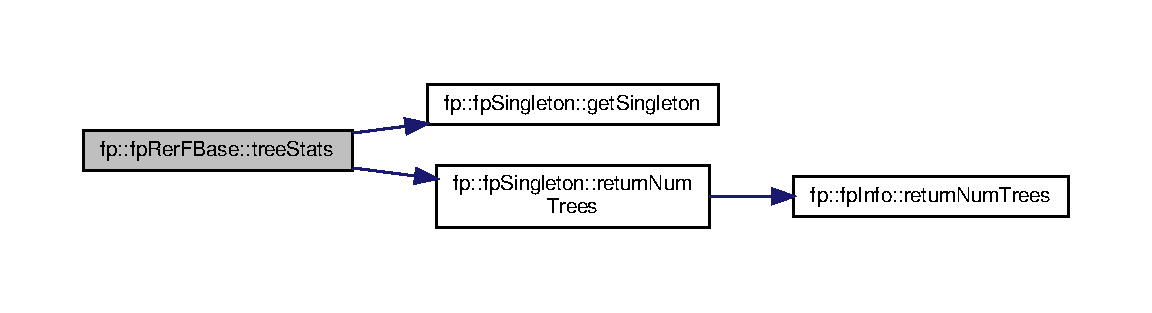
\includegraphics[width=350pt]{classfp_1_1fpRerFBase_ad9983abf38c0cb799ed490129508d42e_cgraph}
\end{center}
\end{figure}


\subsection{Member Data Documentation}
\mbox{\Hypertarget{classfp_1_1fpRerFBase_a539e79a960846182fc49420d79896ba1}\label{classfp_1_1fpRerFBase_a539e79a960846182fc49420d79896ba1}} 
\index{fp\+::fp\+Rer\+F\+Base@{fp\+::fp\+Rer\+F\+Base}!print\+Progress@{print\+Progress}}
\index{print\+Progress@{print\+Progress}!fp\+::fp\+Rer\+F\+Base@{fp\+::fp\+Rer\+F\+Base}}
\subsubsection{\texorpdfstring{print\+Progress}{printProgress}}
{\footnotesize\ttfamily template$<$typename T $>$ \\
\hyperlink{classfp_1_1fpDisplayProgress}{fp\+Display\+Progress} \hyperlink{classfp_1_1fpRerFBase}{fp\+::fp\+Rer\+F\+Base}$<$ T $>$\+::print\+Progress}



Definition at line 27 of file fp\+Rer\+F\+Base.\+h.

\mbox{\Hypertarget{classfp_1_1fpRerFBase_a6c2f12312e64e5234fc53741f1bfbe96}\label{classfp_1_1fpRerFBase_a6c2f12312e64e5234fc53741f1bfbe96}} 
\index{fp\+::fp\+Rer\+F\+Base@{fp\+::fp\+Rer\+F\+Base}!trees@{trees}}
\index{trees@{trees}!fp\+::fp\+Rer\+F\+Base@{fp\+::fp\+Rer\+F\+Base}}
\subsubsection{\texorpdfstring{trees}{trees}}
{\footnotesize\ttfamily template$<$typename T $>$ \\
std\+::vector$<$\hyperlink{classfp_1_1rerfTree}{rerf\+Tree}$<$T$>$ $>$ \hyperlink{classfp_1_1fpRerFBase}{fp\+::fp\+Rer\+F\+Base}$<$ T $>$\+::trees\hspace{0.3cm}{\ttfamily [protected]}}



Definition at line 19 of file fp\+Rer\+F\+Base.\+h.



The documentation for this class was generated from the following file\+:\begin{DoxyCompactItemize}
\item 
src/forest\+Types/rerf/\hyperlink{fpRerFBase_8h}{fp\+Rer\+F\+Base.\+h}\end{DoxyCompactItemize}

\hypertarget{classfp_1_1fpSingleton}{}\section{fp\+:\+:fp\+Singleton Class Reference}
\label{classfp_1_1fpSingleton}\index{fp\+::fp\+Singleton@{fp\+::fp\+Singleton}}


{\ttfamily \#include $<$fp\+Singleton.\+h$>$}



Collaboration diagram for fp\+:\+:fp\+Singleton\+:\nopagebreak
\begin{figure}[H]
\begin{center}
\leavevmode
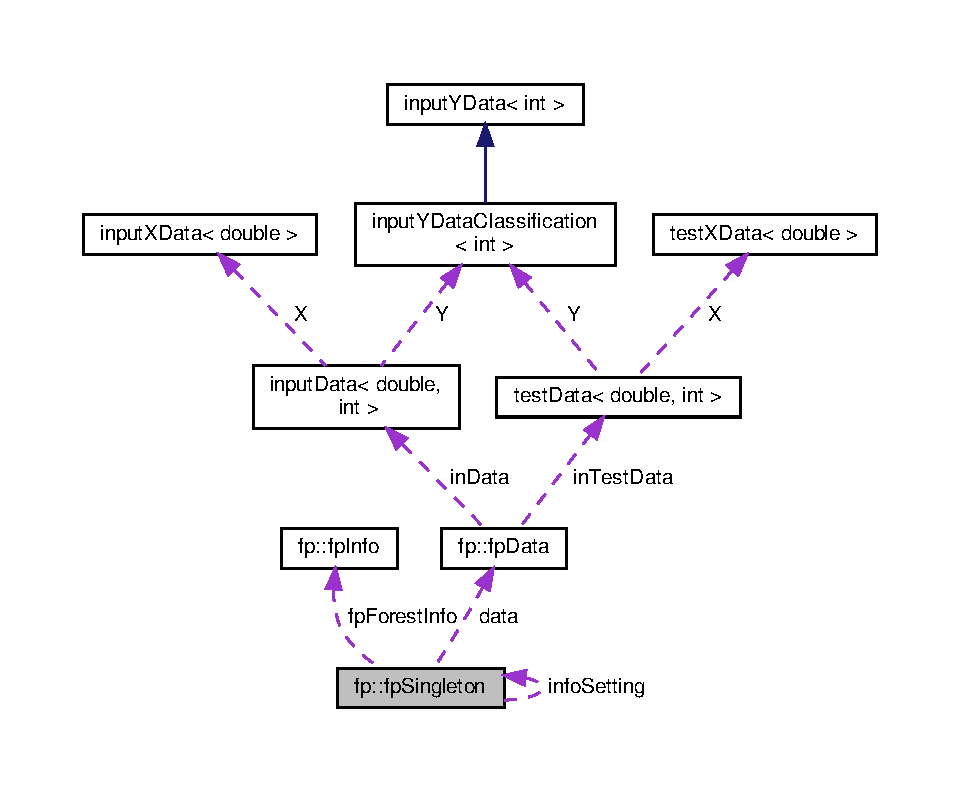
\includegraphics[width=350pt]{classfp_1_1fpSingleton__coll__graph}
\end{center}
\end{figure}
\subsection*{Public Member Functions}
\begin{DoxyCompactItemize}
\item 
void \hyperlink{classfp_1_1fpSingleton_a90f275b256694ea7b16577d547a33044}{set\+Parameter} (const std\+::string \&parameter\+Name, const std\+::string \&parameter\+Value)
\item 
void \hyperlink{classfp_1_1fpSingleton_a19dd80e98acb4dd3e82be5e744840d1f}{set\+Parameter} (const std\+::string \&parameter\+Name, const double parameter\+Value)
\item 
void \hyperlink{classfp_1_1fpSingleton_a3465c3ff9376fae2933d9267c32761ca}{set\+Parameter} (const std\+::string \&parameter\+Name, const int parameter\+Value)
\item 
void \hyperlink{classfp_1_1fpSingleton_a0d769b6652e4c74c2734cdc811eeab5a}{print\+All\+Parameters} ()
\item 
void \hyperlink{classfp_1_1fpSingleton_ad9696336521f72c7c6a021608799871e}{print\+Forest\+Type} ()
\item 
void \hyperlink{classfp_1_1fpSingleton_a86042ae6be6f59dfb90232678350011a}{load\+Data} ()
\item 
void \hyperlink{classfp_1_1fpSingleton_aea7c3b65ded387322d7d5ce48ab96215}{load\+Test\+Data} ()
\item 
void \hyperlink{classfp_1_1fpSingleton_a204b85f9d08ca711ca6620b5e020cc1c}{delete\+Data} ()
\item 
void \hyperlink{classfp_1_1fpSingleton_aa4ac02c580b06ba16ed0160ec694438d}{delete\+Test\+Data} ()
\item 
void \hyperlink{classfp_1_1fpSingleton_a5a35867349f6d172f77af7026fdaecbe}{set\+Num\+Features} (int numF)
\item 
void \hyperlink{classfp_1_1fpSingleton_acf821a8fda9d3296cde7dc33b9c1ddb5}{set\+Num\+Observations} (int numO)
\item 
void \hyperlink{classfp_1_1fpSingleton_a499e7cef6b463cc24590d05a0d0e6e1c}{set\+Num\+Classes} (int numC)
\item 
int \hyperlink{classfp_1_1fpSingleton_a5602580110329a6b25602b1789e4e2c2}{return\+Num\+Classes} ()
\item 
int \hyperlink{classfp_1_1fpSingleton_a45ae68ceb91880ddbc0e049a47c371eb}{return\+Mtry} ()
\item 
std\+::string \& \hyperlink{classfp_1_1fpSingleton_af7582b20b48b7eb8c0a6b89fbdf170ab}{return\+Forest\+Type} ()
\item 
int \hyperlink{classfp_1_1fpSingleton_a97cbcad5ae9daa8c747fd4db84928c20}{return\+Num\+Features} ()
\item 
int \hyperlink{classfp_1_1fpSingleton_ae12f22ad096ff0d419fce47df710bf78}{return\+Num\+Observations} ()
\item 
int \hyperlink{classfp_1_1fpSingleton_aa2f644b1521948fb994f4087ddfaea14}{return\+Label} (int observation\+Number)
\item 
int \hyperlink{classfp_1_1fpSingleton_ac0d2a2fd5ed471c8d507dfd544c12e6d}{return\+Test\+Label} (int observation\+Number)
\item 
double \hyperlink{classfp_1_1fpSingleton_aacc2eb894a219e2fe234743b51fa1a76}{return\+Feature\+Val} (const int feature\+Number, const int observation\+Number)
\item 
void \hyperlink{classfp_1_1fpSingleton_ab789c4e4bfb3248711a5857015008f8d}{prefetch\+Feature\+Val} (const int feature\+Number, const int observation\+Number)
\item 
double \hyperlink{classfp_1_1fpSingleton_ad74b421d65b17ba924244bff31fc9db6}{return\+Test\+Feature\+Val} (const int feature\+Number, const int observation\+Number)
\item 
int \hyperlink{classfp_1_1fpSingleton_a8be36616345b6b77ce4c60b99cc2b91c}{return\+Num\+Trees} ()
\item 
int \hyperlink{classfp_1_1fpSingleton_a2d06406b6462099e0adb393218090420}{return\+Min\+Parent} ()
\item 
void \hyperlink{classfp_1_1fpSingleton_a3edf17209500e72c76ef816e32666eb2}{set\+Data\+Dependent\+Parameters} ()
\item 
bool \hyperlink{classfp_1_1fpSingleton_a12178de58f19494062efe5255d937171}{load\+Data\+From\+C\+SV} ()
\end{DoxyCompactItemize}
\subsection*{Static Public Member Functions}
\begin{DoxyCompactItemize}
\item 
static \hyperlink{classfp_1_1fpSingleton}{fp\+Singleton} \& \hyperlink{classfp_1_1fpSingleton_a8bdae77b68521003e3fc630edec2e240}{get\+Singleton} ()
\end{DoxyCompactItemize}
\subsection*{Private Member Functions}
\begin{DoxyCompactItemize}
\item 
\hyperlink{classfp_1_1fpSingleton_a049e41d4468d9b9f1e08788592c5f4cd}{fp\+Singleton} ()
\item 
\hyperlink{classfp_1_1fpSingleton_a5ea4d9f5a5811e9d9a64581dea9f561a}{$\sim$fp\+Singleton} ()
\item 
\hyperlink{classfp_1_1fpSingleton_afa7b24ca92c18b7e0f444592c9d8ba30}{fp\+Singleton} (const \hyperlink{classfp_1_1fpSingleton}{fp\+Singleton} \&old)
\item 
const \hyperlink{classfp_1_1fpSingleton}{fp\+Singleton} \& \hyperlink{classfp_1_1fpSingleton_a342b8b19aa98af5b2f56210cf0b164b0}{operator=} (const \hyperlink{classfp_1_1fpSingleton}{fp\+Singleton} \&old)
\end{DoxyCompactItemize}
\subsection*{Private Attributes}
\begin{DoxyCompactItemize}
\item 
\hyperlink{classfp_1_1fpInfo}{fp\+Info} \hyperlink{classfp_1_1fpSingleton_a85965009befa72a749ae498fa5b6ccfa}{fp\+Forest\+Info}
\item 
\hyperlink{classfp_1_1fpData}{fp\+Data} \hyperlink{classfp_1_1fpSingleton_a2fa16ac6a0f66641749032eeee61b8e9}{data}
\end{DoxyCompactItemize}
\subsection*{Static Private Attributes}
\begin{DoxyCompactItemize}
\item 
static \hyperlink{classfp_1_1fpSingleton}{fp\+Singleton} $\ast$ \hyperlink{classfp_1_1fpSingleton_a0e2c02e7e7f730f59e5c1f10005d581c}{info\+Setting} = nullptr
\end{DoxyCompactItemize}


\subsection{Detailed Description}


Definition at line 11 of file fp\+Singleton.\+h.



\subsection{Constructor \& Destructor Documentation}
\mbox{\Hypertarget{classfp_1_1fpSingleton_a049e41d4468d9b9f1e08788592c5f4cd}\label{classfp_1_1fpSingleton_a049e41d4468d9b9f1e08788592c5f4cd}} 
\index{fp\+::fp\+Singleton@{fp\+::fp\+Singleton}!fp\+Singleton@{fp\+Singleton}}
\index{fp\+Singleton@{fp\+Singleton}!fp\+::fp\+Singleton@{fp\+::fp\+Singleton}}
\subsubsection{\texorpdfstring{fp\+Singleton()}{fpSingleton()}\hspace{0.1cm}{\footnotesize\ttfamily [1/2]}}
{\footnotesize\ttfamily fp\+::fp\+Singleton\+::fp\+Singleton (\begin{DoxyParamCaption}{ }\end{DoxyParamCaption})\hspace{0.3cm}{\ttfamily [inline]}, {\ttfamily [private]}}



Definition at line 130 of file fp\+Singleton.\+h.


\begin{DoxyCode}
130 \{\}
\end{DoxyCode}
Here is the call graph for this function\+:\nopagebreak
\begin{figure}[H]
\begin{center}
\leavevmode
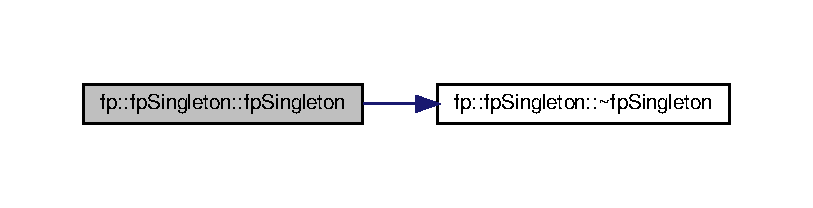
\includegraphics[width=350pt]{classfp_1_1fpSingleton_a049e41d4468d9b9f1e08788592c5f4cd_cgraph}
\end{center}
\end{figure}
\mbox{\Hypertarget{classfp_1_1fpSingleton_a5ea4d9f5a5811e9d9a64581dea9f561a}\label{classfp_1_1fpSingleton_a5ea4d9f5a5811e9d9a64581dea9f561a}} 
\index{fp\+::fp\+Singleton@{fp\+::fp\+Singleton}!````~fp\+Singleton@{$\sim$fp\+Singleton}}
\index{````~fp\+Singleton@{$\sim$fp\+Singleton}!fp\+::fp\+Singleton@{fp\+::fp\+Singleton}}
\subsubsection{\texorpdfstring{$\sim$fp\+Singleton()}{~fpSingleton()}}
{\footnotesize\ttfamily fp\+::fp\+Singleton\+::$\sim$fp\+Singleton (\begin{DoxyParamCaption}{ }\end{DoxyParamCaption})\hspace{0.3cm}{\ttfamily [private]}}

\mbox{\Hypertarget{classfp_1_1fpSingleton_afa7b24ca92c18b7e0f444592c9d8ba30}\label{classfp_1_1fpSingleton_afa7b24ca92c18b7e0f444592c9d8ba30}} 
\index{fp\+::fp\+Singleton@{fp\+::fp\+Singleton}!fp\+Singleton@{fp\+Singleton}}
\index{fp\+Singleton@{fp\+Singleton}!fp\+::fp\+Singleton@{fp\+::fp\+Singleton}}
\subsubsection{\texorpdfstring{fp\+Singleton()}{fpSingleton()}\hspace{0.1cm}{\footnotesize\ttfamily [2/2]}}
{\footnotesize\ttfamily fp\+::fp\+Singleton\+::fp\+Singleton (\begin{DoxyParamCaption}\item[{const \hyperlink{classfp_1_1fpSingleton}{fp\+Singleton} \&}]{old }\end{DoxyParamCaption})\hspace{0.3cm}{\ttfamily [inline]}, {\ttfamily [private]}}



Definition at line 132 of file fp\+Singleton.\+h.


\begin{DoxyCode}
132                                                \{
133                 \textcolor{keywordflow}{if}(\textcolor{keyword}{this} != &old)\{
134                     \hyperlink{classfp_1_1fpSingleton_a0e2c02e7e7f730f59e5c1f10005d581c}{infoSetting}= old.\hyperlink{classfp_1_1fpSingleton_a0e2c02e7e7f730f59e5c1f10005d581c}{infoSetting};
135                 \}
136             \}
\end{DoxyCode}


\subsection{Member Function Documentation}
\mbox{\Hypertarget{classfp_1_1fpSingleton_a204b85f9d08ca711ca6620b5e020cc1c}\label{classfp_1_1fpSingleton_a204b85f9d08ca711ca6620b5e020cc1c}} 
\index{fp\+::fp\+Singleton@{fp\+::fp\+Singleton}!delete\+Data@{delete\+Data}}
\index{delete\+Data@{delete\+Data}!fp\+::fp\+Singleton@{fp\+::fp\+Singleton}}
\subsubsection{\texorpdfstring{delete\+Data()}{deleteData()}}
{\footnotesize\ttfamily void fp\+::fp\+Singleton\+::delete\+Data (\begin{DoxyParamCaption}{ }\end{DoxyParamCaption})\hspace{0.3cm}{\ttfamily [inline]}}



Definition at line 52 of file fp\+Singleton.\+h.


\begin{DoxyCode}
52                                     \{
53                 \hyperlink{classfp_1_1fpSingleton_a2fa16ac6a0f66641749032eeee61b8e9}{data}.\hyperlink{classfp_1_1fpData_a44df119acad6c339966d67f2c634a369}{fpDeleteData}();
54             \}
\end{DoxyCode}
Here is the call graph for this function\+:\nopagebreak
\begin{figure}[H]
\begin{center}
\leavevmode
\includegraphics[width=350pt]{classfp_1_1fpSingleton_a204b85f9d08ca711ca6620b5e020cc1c_cgraph}
\end{center}
\end{figure}
\mbox{\Hypertarget{classfp_1_1fpSingleton_aa4ac02c580b06ba16ed0160ec694438d}\label{classfp_1_1fpSingleton_aa4ac02c580b06ba16ed0160ec694438d}} 
\index{fp\+::fp\+Singleton@{fp\+::fp\+Singleton}!delete\+Test\+Data@{delete\+Test\+Data}}
\index{delete\+Test\+Data@{delete\+Test\+Data}!fp\+::fp\+Singleton@{fp\+::fp\+Singleton}}
\subsubsection{\texorpdfstring{delete\+Test\+Data()}{deleteTestData()}}
{\footnotesize\ttfamily void fp\+::fp\+Singleton\+::delete\+Test\+Data (\begin{DoxyParamCaption}{ }\end{DoxyParamCaption})\hspace{0.3cm}{\ttfamily [inline]}}



Definition at line 56 of file fp\+Singleton.\+h.


\begin{DoxyCode}
56                                         \{
57                 \hyperlink{classfp_1_1fpSingleton_a2fa16ac6a0f66641749032eeee61b8e9}{data}.\hyperlink{classfp_1_1fpData_a996eedfc5ffe559ce1f6061af1efc1db}{fpDeleteTestData}();
58             \}
\end{DoxyCode}
Here is the call graph for this function\+:\nopagebreak
\begin{figure}[H]
\begin{center}
\leavevmode
\includegraphics[width=350pt]{classfp_1_1fpSingleton_aa4ac02c580b06ba16ed0160ec694438d_cgraph}
\end{center}
\end{figure}
\mbox{\Hypertarget{classfp_1_1fpSingleton_a8bdae77b68521003e3fc630edec2e240}\label{classfp_1_1fpSingleton_a8bdae77b68521003e3fc630edec2e240}} 
\index{fp\+::fp\+Singleton@{fp\+::fp\+Singleton}!get\+Singleton@{get\+Singleton}}
\index{get\+Singleton@{get\+Singleton}!fp\+::fp\+Singleton@{fp\+::fp\+Singleton}}
\subsubsection{\texorpdfstring{get\+Singleton()}{getSingleton()}}
{\footnotesize\ttfamily static \hyperlink{classfp_1_1fpSingleton}{fp\+Singleton}\& fp\+::fp\+Singleton\+::get\+Singleton (\begin{DoxyParamCaption}{ }\end{DoxyParamCaption})\hspace{0.3cm}{\ttfamily [inline]}, {\ttfamily [static]}}



Definition at line 19 of file fp\+Singleton.\+h.


\begin{DoxyCode}
19                                               \{
20                 \textcolor{keyword}{static} \hyperlink{classfp_1_1fpSingleton_a049e41d4468d9b9f1e08788592c5f4cd}{fpSingleton}* \hyperlink{classfp_1_1fpSingleton_a0e2c02e7e7f730f59e5c1f10005d581c}{infoSetting}(\textcolor{keyword}{new} 
      \hyperlink{classfp_1_1fpSingleton_a049e41d4468d9b9f1e08788592c5f4cd}{fpSingleton});
21                 \textcolor{keywordflow}{return} *\hyperlink{classfp_1_1fpSingleton_a0e2c02e7e7f730f59e5c1f10005d581c}{infoSetting};
22             \}
\end{DoxyCode}
\mbox{\Hypertarget{classfp_1_1fpSingleton_a86042ae6be6f59dfb90232678350011a}\label{classfp_1_1fpSingleton_a86042ae6be6f59dfb90232678350011a}} 
\index{fp\+::fp\+Singleton@{fp\+::fp\+Singleton}!load\+Data@{load\+Data}}
\index{load\+Data@{load\+Data}!fp\+::fp\+Singleton@{fp\+::fp\+Singleton}}
\subsubsection{\texorpdfstring{load\+Data()}{loadData()}}
{\footnotesize\ttfamily void fp\+::fp\+Singleton\+::load\+Data (\begin{DoxyParamCaption}{ }\end{DoxyParamCaption})\hspace{0.3cm}{\ttfamily [inline]}}



Definition at line 44 of file fp\+Singleton.\+h.


\begin{DoxyCode}
44                                   \{
45                 \hyperlink{classfp_1_1fpSingleton_a2fa16ac6a0f66641749032eeee61b8e9}{data}.\hyperlink{classfp_1_1fpData_a91c727b1475eca340ca14c241b25c959}{fpLoadData}(\hyperlink{classfp_1_1fpSingleton_a85965009befa72a749ae498fa5b6ccfa}{fpForestInfo});
46             \}
\end{DoxyCode}
Here is the call graph for this function\+:\nopagebreak
\begin{figure}[H]
\begin{center}
\leavevmode
\includegraphics[width=350pt]{classfp_1_1fpSingleton_a86042ae6be6f59dfb90232678350011a_cgraph}
\end{center}
\end{figure}
\mbox{\Hypertarget{classfp_1_1fpSingleton_a12178de58f19494062efe5255d937171}\label{classfp_1_1fpSingleton_a12178de58f19494062efe5255d937171}} 
\index{fp\+::fp\+Singleton@{fp\+::fp\+Singleton}!load\+Data\+From\+C\+SV@{load\+Data\+From\+C\+SV}}
\index{load\+Data\+From\+C\+SV@{load\+Data\+From\+C\+SV}!fp\+::fp\+Singleton@{fp\+::fp\+Singleton}}
\subsubsection{\texorpdfstring{load\+Data\+From\+C\+S\+V()}{loadDataFromCSV()}}
{\footnotesize\ttfamily bool fp\+::fp\+Singleton\+::load\+Data\+From\+C\+SV (\begin{DoxyParamCaption}{ }\end{DoxyParamCaption})\hspace{0.3cm}{\ttfamily [inline]}}



Definition at line 125 of file fp\+Singleton.\+h.


\begin{DoxyCode}
125                                          \{
126                 \textcolor{keywordflow}{return} \hyperlink{classfp_1_1fpSingleton_a2fa16ac6a0f66641749032eeee61b8e9}{data}.\hyperlink{classfp_1_1fpData_a2b4d9be328aaa7acf9a2561150da0402}{loadDataFromCSV}(\hyperlink{classfp_1_1fpSingleton_a85965009befa72a749ae498fa5b6ccfa}{fpForestInfo});
127             \}
\end{DoxyCode}
Here is the call graph for this function\+:\nopagebreak
\begin{figure}[H]
\begin{center}
\leavevmode
\includegraphics[width=350pt]{classfp_1_1fpSingleton_a12178de58f19494062efe5255d937171_cgraph}
\end{center}
\end{figure}
\mbox{\Hypertarget{classfp_1_1fpSingleton_aea7c3b65ded387322d7d5ce48ab96215}\label{classfp_1_1fpSingleton_aea7c3b65ded387322d7d5ce48ab96215}} 
\index{fp\+::fp\+Singleton@{fp\+::fp\+Singleton}!load\+Test\+Data@{load\+Test\+Data}}
\index{load\+Test\+Data@{load\+Test\+Data}!fp\+::fp\+Singleton@{fp\+::fp\+Singleton}}
\subsubsection{\texorpdfstring{load\+Test\+Data()}{loadTestData()}}
{\footnotesize\ttfamily void fp\+::fp\+Singleton\+::load\+Test\+Data (\begin{DoxyParamCaption}{ }\end{DoxyParamCaption})\hspace{0.3cm}{\ttfamily [inline]}}



Definition at line 48 of file fp\+Singleton.\+h.


\begin{DoxyCode}
48                                       \{
49                 \hyperlink{classfp_1_1fpSingleton_a2fa16ac6a0f66641749032eeee61b8e9}{data}.\hyperlink{classfp_1_1fpData_a4b527bc84762c4708992b7fdce3d0602}{fpLoadTestData}(\hyperlink{classfp_1_1fpSingleton_a85965009befa72a749ae498fa5b6ccfa}{fpForestInfo});
50             \}
\end{DoxyCode}
Here is the call graph for this function\+:\nopagebreak
\begin{figure}[H]
\begin{center}
\leavevmode
\includegraphics[width=350pt]{classfp_1_1fpSingleton_aea7c3b65ded387322d7d5ce48ab96215_cgraph}
\end{center}
\end{figure}
\mbox{\Hypertarget{classfp_1_1fpSingleton_a342b8b19aa98af5b2f56210cf0b164b0}\label{classfp_1_1fpSingleton_a342b8b19aa98af5b2f56210cf0b164b0}} 
\index{fp\+::fp\+Singleton@{fp\+::fp\+Singleton}!operator=@{operator=}}
\index{operator=@{operator=}!fp\+::fp\+Singleton@{fp\+::fp\+Singleton}}
\subsubsection{\texorpdfstring{operator=()}{operator=()}}
{\footnotesize\ttfamily const \hyperlink{classfp_1_1fpSingleton}{fp\+Singleton}\& fp\+::fp\+Singleton\+::operator= (\begin{DoxyParamCaption}\item[{const \hyperlink{classfp_1_1fpSingleton}{fp\+Singleton} \&}]{old }\end{DoxyParamCaption})\hspace{0.3cm}{\ttfamily [inline]}, {\ttfamily [private]}}



Definition at line 137 of file fp\+Singleton.\+h.


\begin{DoxyCode}
137                                                                 \{
138                 \textcolor{keywordflow}{if}(\textcolor{keyword}{this} !=&old)\{
139                     \hyperlink{classfp_1_1fpSingleton_a0e2c02e7e7f730f59e5c1f10005d581c}{infoSetting}=old.\hyperlink{classfp_1_1fpSingleton_a0e2c02e7e7f730f59e5c1f10005d581c}{infoSetting};
140                 \}
141                 \textcolor{keywordflow}{return} *\textcolor{keyword}{this};
142             \}
\end{DoxyCode}
\mbox{\Hypertarget{classfp_1_1fpSingleton_ab789c4e4bfb3248711a5857015008f8d}\label{classfp_1_1fpSingleton_ab789c4e4bfb3248711a5857015008f8d}} 
\index{fp\+::fp\+Singleton@{fp\+::fp\+Singleton}!prefetch\+Feature\+Val@{prefetch\+Feature\+Val}}
\index{prefetch\+Feature\+Val@{prefetch\+Feature\+Val}!fp\+::fp\+Singleton@{fp\+::fp\+Singleton}}
\subsubsection{\texorpdfstring{prefetch\+Feature\+Val()}{prefetchFeatureVal()}}
{\footnotesize\ttfamily void fp\+::fp\+Singleton\+::prefetch\+Feature\+Val (\begin{DoxyParamCaption}\item[{const int}]{feature\+Number,  }\item[{const int}]{observation\+Number }\end{DoxyParamCaption})\hspace{0.3cm}{\ttfamily [inline]}}



Definition at line 105 of file fp\+Singleton.\+h.


\begin{DoxyCode}
105                                                                                     \{
106                 \hyperlink{classfp_1_1fpSingleton_a2fa16ac6a0f66641749032eeee61b8e9}{data}.\hyperlink{classfp_1_1fpData_a3f9645ca93e9b64a788b3042e9e41fcc}{prefetchFeatureVal}(featureNumber, observationNumber);
107             \}
\end{DoxyCode}
Here is the call graph for this function\+:\nopagebreak
\begin{figure}[H]
\begin{center}
\leavevmode
\includegraphics[width=350pt]{classfp_1_1fpSingleton_ab789c4e4bfb3248711a5857015008f8d_cgraph}
\end{center}
\end{figure}
\mbox{\Hypertarget{classfp_1_1fpSingleton_a0d769b6652e4c74c2734cdc811eeab5a}\label{classfp_1_1fpSingleton_a0d769b6652e4c74c2734cdc811eeab5a}} 
\index{fp\+::fp\+Singleton@{fp\+::fp\+Singleton}!print\+All\+Parameters@{print\+All\+Parameters}}
\index{print\+All\+Parameters@{print\+All\+Parameters}!fp\+::fp\+Singleton@{fp\+::fp\+Singleton}}
\subsubsection{\texorpdfstring{print\+All\+Parameters()}{printAllParameters()}}
{\footnotesize\ttfamily void fp\+::fp\+Singleton\+::print\+All\+Parameters (\begin{DoxyParamCaption}{ }\end{DoxyParamCaption})\hspace{0.3cm}{\ttfamily [inline]}}



Definition at line 36 of file fp\+Singleton.\+h.


\begin{DoxyCode}
36                                             \{
37                 \hyperlink{classfp_1_1fpSingleton_a85965009befa72a749ae498fa5b6ccfa}{fpForestInfo}.\hyperlink{classfp_1_1fpInfo_a471bd46c828547d5b556f6f4e9fca70f}{printAllParameters}();
38             \}
\end{DoxyCode}
Here is the call graph for this function\+:\nopagebreak
\begin{figure}[H]
\begin{center}
\leavevmode
\includegraphics[width=350pt]{classfp_1_1fpSingleton_a0d769b6652e4c74c2734cdc811eeab5a_cgraph}
\end{center}
\end{figure}
\mbox{\Hypertarget{classfp_1_1fpSingleton_ad9696336521f72c7c6a021608799871e}\label{classfp_1_1fpSingleton_ad9696336521f72c7c6a021608799871e}} 
\index{fp\+::fp\+Singleton@{fp\+::fp\+Singleton}!print\+Forest\+Type@{print\+Forest\+Type}}
\index{print\+Forest\+Type@{print\+Forest\+Type}!fp\+::fp\+Singleton@{fp\+::fp\+Singleton}}
\subsubsection{\texorpdfstring{print\+Forest\+Type()}{printForestType()}}
{\footnotesize\ttfamily void fp\+::fp\+Singleton\+::print\+Forest\+Type (\begin{DoxyParamCaption}{ }\end{DoxyParamCaption})\hspace{0.3cm}{\ttfamily [inline]}}



Definition at line 40 of file fp\+Singleton.\+h.


\begin{DoxyCode}
40                                          \{
41                 \hyperlink{classfp_1_1fpSingleton_a85965009befa72a749ae498fa5b6ccfa}{fpForestInfo}.\hyperlink{classfp_1_1fpInfo_a1acfffe3b13e5cad548f92cd09ff7f46}{printForestType}();
42             \}
\end{DoxyCode}
Here is the call graph for this function\+:\nopagebreak
\begin{figure}[H]
\begin{center}
\leavevmode
\includegraphics[width=350pt]{classfp_1_1fpSingleton_ad9696336521f72c7c6a021608799871e_cgraph}
\end{center}
\end{figure}
\mbox{\Hypertarget{classfp_1_1fpSingleton_aacc2eb894a219e2fe234743b51fa1a76}\label{classfp_1_1fpSingleton_aacc2eb894a219e2fe234743b51fa1a76}} 
\index{fp\+::fp\+Singleton@{fp\+::fp\+Singleton}!return\+Feature\+Val@{return\+Feature\+Val}}
\index{return\+Feature\+Val@{return\+Feature\+Val}!fp\+::fp\+Singleton@{fp\+::fp\+Singleton}}
\subsubsection{\texorpdfstring{return\+Feature\+Val()}{returnFeatureVal()}}
{\footnotesize\ttfamily double fp\+::fp\+Singleton\+::return\+Feature\+Val (\begin{DoxyParamCaption}\item[{const int}]{feature\+Number,  }\item[{const int}]{observation\+Number }\end{DoxyParamCaption})\hspace{0.3cm}{\ttfamily [inline]}}



Definition at line 101 of file fp\+Singleton.\+h.


\begin{DoxyCode}
101                                                                                                 \{
102                 \textcolor{keywordflow}{return} \hyperlink{classfp_1_1fpSingleton_a2fa16ac6a0f66641749032eeee61b8e9}{data}.\hyperlink{classfp_1_1fpData_a6b359086ec1e5c534095600e2ed5575f}{returnFeatureVal}(featureNumber, observationNumber);
103             \}
\end{DoxyCode}
Here is the call graph for this function\+:\nopagebreak
\begin{figure}[H]
\begin{center}
\leavevmode
\includegraphics[width=350pt]{classfp_1_1fpSingleton_aacc2eb894a219e2fe234743b51fa1a76_cgraph}
\end{center}
\end{figure}
\mbox{\Hypertarget{classfp_1_1fpSingleton_af7582b20b48b7eb8c0a6b89fbdf170ab}\label{classfp_1_1fpSingleton_af7582b20b48b7eb8c0a6b89fbdf170ab}} 
\index{fp\+::fp\+Singleton@{fp\+::fp\+Singleton}!return\+Forest\+Type@{return\+Forest\+Type}}
\index{return\+Forest\+Type@{return\+Forest\+Type}!fp\+::fp\+Singleton@{fp\+::fp\+Singleton}}
\subsubsection{\texorpdfstring{return\+Forest\+Type()}{returnForestType()}}
{\footnotesize\ttfamily std\+::string\& fp\+::fp\+Singleton\+::return\+Forest\+Type (\begin{DoxyParamCaption}{ }\end{DoxyParamCaption})\hspace{0.3cm}{\ttfamily [inline]}}



Definition at line 81 of file fp\+Singleton.\+h.


\begin{DoxyCode}
81                                                 \{
82                 \textcolor{keywordflow}{return} \hyperlink{classfp_1_1fpSingleton_a85965009befa72a749ae498fa5b6ccfa}{fpForestInfo}.\hyperlink{classfp_1_1fpInfo_a97280e7e3cadc5e653d8ef256eb2c82d}{returnForestType}();
83             \}
\end{DoxyCode}
Here is the call graph for this function\+:\nopagebreak
\begin{figure}[H]
\begin{center}
\leavevmode
\includegraphics[width=350pt]{classfp_1_1fpSingleton_af7582b20b48b7eb8c0a6b89fbdf170ab_cgraph}
\end{center}
\end{figure}
\mbox{\Hypertarget{classfp_1_1fpSingleton_aa2f644b1521948fb994f4087ddfaea14}\label{classfp_1_1fpSingleton_aa2f644b1521948fb994f4087ddfaea14}} 
\index{fp\+::fp\+Singleton@{fp\+::fp\+Singleton}!return\+Label@{return\+Label}}
\index{return\+Label@{return\+Label}!fp\+::fp\+Singleton@{fp\+::fp\+Singleton}}
\subsubsection{\texorpdfstring{return\+Label()}{returnLabel()}}
{\footnotesize\ttfamily int fp\+::fp\+Singleton\+::return\+Label (\begin{DoxyParamCaption}\item[{int}]{observation\+Number }\end{DoxyParamCaption})\hspace{0.3cm}{\ttfamily [inline]}}



Definition at line 93 of file fp\+Singleton.\+h.


\begin{DoxyCode}
93                                                          \{
94                 \textcolor{keywordflow}{return} \hyperlink{classfp_1_1fpSingleton_a2fa16ac6a0f66641749032eeee61b8e9}{data}.\hyperlink{classfp_1_1fpData_aac722f51424cb7f6ab7d89525f82cc72}{returnLabel}(observationNumber);
95             \}
\end{DoxyCode}
Here is the call graph for this function\+:\nopagebreak
\begin{figure}[H]
\begin{center}
\leavevmode
\includegraphics[width=350pt]{classfp_1_1fpSingleton_aa2f644b1521948fb994f4087ddfaea14_cgraph}
\end{center}
\end{figure}
\mbox{\Hypertarget{classfp_1_1fpSingleton_a2d06406b6462099e0adb393218090420}\label{classfp_1_1fpSingleton_a2d06406b6462099e0adb393218090420}} 
\index{fp\+::fp\+Singleton@{fp\+::fp\+Singleton}!return\+Min\+Parent@{return\+Min\+Parent}}
\index{return\+Min\+Parent@{return\+Min\+Parent}!fp\+::fp\+Singleton@{fp\+::fp\+Singleton}}
\subsubsection{\texorpdfstring{return\+Min\+Parent()}{returnMinParent()}}
{\footnotesize\ttfamily int fp\+::fp\+Singleton\+::return\+Min\+Parent (\begin{DoxyParamCaption}{ }\end{DoxyParamCaption})\hspace{0.3cm}{\ttfamily [inline]}}



Definition at line 117 of file fp\+Singleton.\+h.


\begin{DoxyCode}
117                                         \{
118                 \textcolor{keywordflow}{return} \hyperlink{classfp_1_1fpSingleton_a85965009befa72a749ae498fa5b6ccfa}{fpForestInfo}.\hyperlink{classfp_1_1fpInfo_ad1af845e85cb6e807694c5106baca230}{returnMinParent}();
119             \}
\end{DoxyCode}
Here is the call graph for this function\+:\nopagebreak
\begin{figure}[H]
\begin{center}
\leavevmode
\includegraphics[width=350pt]{classfp_1_1fpSingleton_a2d06406b6462099e0adb393218090420_cgraph}
\end{center}
\end{figure}
\mbox{\Hypertarget{classfp_1_1fpSingleton_a45ae68ceb91880ddbc0e049a47c371eb}\label{classfp_1_1fpSingleton_a45ae68ceb91880ddbc0e049a47c371eb}} 
\index{fp\+::fp\+Singleton@{fp\+::fp\+Singleton}!return\+Mtry@{return\+Mtry}}
\index{return\+Mtry@{return\+Mtry}!fp\+::fp\+Singleton@{fp\+::fp\+Singleton}}
\subsubsection{\texorpdfstring{return\+Mtry()}{returnMtry()}}
{\footnotesize\ttfamily int fp\+::fp\+Singleton\+::return\+Mtry (\begin{DoxyParamCaption}{ }\end{DoxyParamCaption})\hspace{0.3cm}{\ttfamily [inline]}}



Definition at line 77 of file fp\+Singleton.\+h.


\begin{DoxyCode}
77                                    \{
78                 \textcolor{keywordflow}{return} \hyperlink{classfp_1_1fpSingleton_a85965009befa72a749ae498fa5b6ccfa}{fpForestInfo}.\hyperlink{classfp_1_1fpInfo_a058477c4f05818c220efa469b7b630bb}{returnMtry}();
79             \}
\end{DoxyCode}
Here is the call graph for this function\+:\nopagebreak
\begin{figure}[H]
\begin{center}
\leavevmode
\includegraphics[width=350pt]{classfp_1_1fpSingleton_a45ae68ceb91880ddbc0e049a47c371eb_cgraph}
\end{center}
\end{figure}
\mbox{\Hypertarget{classfp_1_1fpSingleton_a5602580110329a6b25602b1789e4e2c2}\label{classfp_1_1fpSingleton_a5602580110329a6b25602b1789e4e2c2}} 
\index{fp\+::fp\+Singleton@{fp\+::fp\+Singleton}!return\+Num\+Classes@{return\+Num\+Classes}}
\index{return\+Num\+Classes@{return\+Num\+Classes}!fp\+::fp\+Singleton@{fp\+::fp\+Singleton}}
\subsubsection{\texorpdfstring{return\+Num\+Classes()}{returnNumClasses()}}
{\footnotesize\ttfamily int fp\+::fp\+Singleton\+::return\+Num\+Classes (\begin{DoxyParamCaption}{ }\end{DoxyParamCaption})\hspace{0.3cm}{\ttfamily [inline]}}



Definition at line 73 of file fp\+Singleton.\+h.


\begin{DoxyCode}
73                                          \{
74                 \textcolor{keywordflow}{return} \hyperlink{classfp_1_1fpSingleton_a85965009befa72a749ae498fa5b6ccfa}{fpForestInfo}.\hyperlink{classfp_1_1fpInfo_a641516fa21a5d6170f74426cf9e2b255}{returnNumClasses}();
75             \}
\end{DoxyCode}
Here is the call graph for this function\+:\nopagebreak
\begin{figure}[H]
\begin{center}
\leavevmode
\includegraphics[width=350pt]{classfp_1_1fpSingleton_a5602580110329a6b25602b1789e4e2c2_cgraph}
\end{center}
\end{figure}
\mbox{\Hypertarget{classfp_1_1fpSingleton_a97cbcad5ae9daa8c747fd4db84928c20}\label{classfp_1_1fpSingleton_a97cbcad5ae9daa8c747fd4db84928c20}} 
\index{fp\+::fp\+Singleton@{fp\+::fp\+Singleton}!return\+Num\+Features@{return\+Num\+Features}}
\index{return\+Num\+Features@{return\+Num\+Features}!fp\+::fp\+Singleton@{fp\+::fp\+Singleton}}
\subsubsection{\texorpdfstring{return\+Num\+Features()}{returnNumFeatures()}}
{\footnotesize\ttfamily int fp\+::fp\+Singleton\+::return\+Num\+Features (\begin{DoxyParamCaption}{ }\end{DoxyParamCaption})\hspace{0.3cm}{\ttfamily [inline]}}



Definition at line 85 of file fp\+Singleton.\+h.


\begin{DoxyCode}
85                                           \{
86                 \textcolor{keywordflow}{return} \hyperlink{classfp_1_1fpSingleton_a85965009befa72a749ae498fa5b6ccfa}{fpForestInfo}.\hyperlink{classfp_1_1fpInfo_abf1e1bfc3e7daa178f3d68bed6311edb}{returnNumFeatures}();
87             \}
\end{DoxyCode}
Here is the call graph for this function\+:\nopagebreak
\begin{figure}[H]
\begin{center}
\leavevmode
\includegraphics[width=350pt]{classfp_1_1fpSingleton_a97cbcad5ae9daa8c747fd4db84928c20_cgraph}
\end{center}
\end{figure}
\mbox{\Hypertarget{classfp_1_1fpSingleton_ae12f22ad096ff0d419fce47df710bf78}\label{classfp_1_1fpSingleton_ae12f22ad096ff0d419fce47df710bf78}} 
\index{fp\+::fp\+Singleton@{fp\+::fp\+Singleton}!return\+Num\+Observations@{return\+Num\+Observations}}
\index{return\+Num\+Observations@{return\+Num\+Observations}!fp\+::fp\+Singleton@{fp\+::fp\+Singleton}}
\subsubsection{\texorpdfstring{return\+Num\+Observations()}{returnNumObservations()}}
{\footnotesize\ttfamily int fp\+::fp\+Singleton\+::return\+Num\+Observations (\begin{DoxyParamCaption}{ }\end{DoxyParamCaption})\hspace{0.3cm}{\ttfamily [inline]}}



Definition at line 89 of file fp\+Singleton.\+h.


\begin{DoxyCode}
89                                               \{
90                 \textcolor{keywordflow}{return} \hyperlink{classfp_1_1fpSingleton_a85965009befa72a749ae498fa5b6ccfa}{fpForestInfo}.\hyperlink{classfp_1_1fpInfo_a5d70dfbd1f8dc26dbd8f066e210cf165}{returnNumObservations}();
91             \}
\end{DoxyCode}
Here is the call graph for this function\+:\nopagebreak
\begin{figure}[H]
\begin{center}
\leavevmode
\includegraphics[width=350pt]{classfp_1_1fpSingleton_ae12f22ad096ff0d419fce47df710bf78_cgraph}
\end{center}
\end{figure}
\mbox{\Hypertarget{classfp_1_1fpSingleton_a8be36616345b6b77ce4c60b99cc2b91c}\label{classfp_1_1fpSingleton_a8be36616345b6b77ce4c60b99cc2b91c}} 
\index{fp\+::fp\+Singleton@{fp\+::fp\+Singleton}!return\+Num\+Trees@{return\+Num\+Trees}}
\index{return\+Num\+Trees@{return\+Num\+Trees}!fp\+::fp\+Singleton@{fp\+::fp\+Singleton}}
\subsubsection{\texorpdfstring{return\+Num\+Trees()}{returnNumTrees()}}
{\footnotesize\ttfamily int fp\+::fp\+Singleton\+::return\+Num\+Trees (\begin{DoxyParamCaption}{ }\end{DoxyParamCaption})\hspace{0.3cm}{\ttfamily [inline]}}



Definition at line 113 of file fp\+Singleton.\+h.


\begin{DoxyCode}
113                                        \{
114                 \textcolor{keywordflow}{return} \hyperlink{classfp_1_1fpSingleton_a85965009befa72a749ae498fa5b6ccfa}{fpForestInfo}.\hyperlink{classfp_1_1fpInfo_a12d3d4b2216f37daf6555f07148c4f85}{returnNumTrees}();
115             \}
\end{DoxyCode}
Here is the call graph for this function\+:\nopagebreak
\begin{figure}[H]
\begin{center}
\leavevmode
\includegraphics[width=350pt]{classfp_1_1fpSingleton_a8be36616345b6b77ce4c60b99cc2b91c_cgraph}
\end{center}
\end{figure}
\mbox{\Hypertarget{classfp_1_1fpSingleton_ad74b421d65b17ba924244bff31fc9db6}\label{classfp_1_1fpSingleton_ad74b421d65b17ba924244bff31fc9db6}} 
\index{fp\+::fp\+Singleton@{fp\+::fp\+Singleton}!return\+Test\+Feature\+Val@{return\+Test\+Feature\+Val}}
\index{return\+Test\+Feature\+Val@{return\+Test\+Feature\+Val}!fp\+::fp\+Singleton@{fp\+::fp\+Singleton}}
\subsubsection{\texorpdfstring{return\+Test\+Feature\+Val()}{returnTestFeatureVal()}}
{\footnotesize\ttfamily double fp\+::fp\+Singleton\+::return\+Test\+Feature\+Val (\begin{DoxyParamCaption}\item[{const int}]{feature\+Number,  }\item[{const int}]{observation\+Number }\end{DoxyParamCaption})\hspace{0.3cm}{\ttfamily [inline]}}



Definition at line 109 of file fp\+Singleton.\+h.


\begin{DoxyCode}
109                                                                                                     \{
110                 \textcolor{keywordflow}{return} \hyperlink{classfp_1_1fpSingleton_a2fa16ac6a0f66641749032eeee61b8e9}{data}.\hyperlink{classfp_1_1fpData_a42f76961f1649e329d654e9e1bb13fc6}{returnTestFeatureVal}(featureNumber, observationNumber);
111             \}
\end{DoxyCode}
Here is the call graph for this function\+:\nopagebreak
\begin{figure}[H]
\begin{center}
\leavevmode
\includegraphics[width=350pt]{classfp_1_1fpSingleton_ad74b421d65b17ba924244bff31fc9db6_cgraph}
\end{center}
\end{figure}
\mbox{\Hypertarget{classfp_1_1fpSingleton_ac0d2a2fd5ed471c8d507dfd544c12e6d}\label{classfp_1_1fpSingleton_ac0d2a2fd5ed471c8d507dfd544c12e6d}} 
\index{fp\+::fp\+Singleton@{fp\+::fp\+Singleton}!return\+Test\+Label@{return\+Test\+Label}}
\index{return\+Test\+Label@{return\+Test\+Label}!fp\+::fp\+Singleton@{fp\+::fp\+Singleton}}
\subsubsection{\texorpdfstring{return\+Test\+Label()}{returnTestLabel()}}
{\footnotesize\ttfamily int fp\+::fp\+Singleton\+::return\+Test\+Label (\begin{DoxyParamCaption}\item[{int}]{observation\+Number }\end{DoxyParamCaption})\hspace{0.3cm}{\ttfamily [inline]}}



Definition at line 97 of file fp\+Singleton.\+h.


\begin{DoxyCode}
97                                                              \{
98                 \textcolor{keywordflow}{return} \hyperlink{classfp_1_1fpSingleton_a2fa16ac6a0f66641749032eeee61b8e9}{data}.\hyperlink{classfp_1_1fpData_a50b6343c52560d1992de50e8cd6b1206}{returnTestLabel}(observationNumber);
99             \}
\end{DoxyCode}
Here is the call graph for this function\+:\nopagebreak
\begin{figure}[H]
\begin{center}
\leavevmode
\includegraphics[width=350pt]{classfp_1_1fpSingleton_ac0d2a2fd5ed471c8d507dfd544c12e6d_cgraph}
\end{center}
\end{figure}
\mbox{\Hypertarget{classfp_1_1fpSingleton_a3edf17209500e72c76ef816e32666eb2}\label{classfp_1_1fpSingleton_a3edf17209500e72c76ef816e32666eb2}} 
\index{fp\+::fp\+Singleton@{fp\+::fp\+Singleton}!set\+Data\+Dependent\+Parameters@{set\+Data\+Dependent\+Parameters}}
\index{set\+Data\+Dependent\+Parameters@{set\+Data\+Dependent\+Parameters}!fp\+::fp\+Singleton@{fp\+::fp\+Singleton}}
\subsubsection{\texorpdfstring{set\+Data\+Dependent\+Parameters()}{setDataDependentParameters()}}
{\footnotesize\ttfamily void fp\+::fp\+Singleton\+::set\+Data\+Dependent\+Parameters (\begin{DoxyParamCaption}{ }\end{DoxyParamCaption})\hspace{0.3cm}{\ttfamily [inline]}}



Definition at line 121 of file fp\+Singleton.\+h.


\begin{DoxyCode}
121                                                     \{
122                 \hyperlink{classfp_1_1fpSingleton_a85965009befa72a749ae498fa5b6ccfa}{fpForestInfo}.\hyperlink{classfp_1_1fpInfo_a6b2a54fb9b3672e7b1bab3474a0ca33f}{setMTRY}();
123             \}
\end{DoxyCode}
Here is the call graph for this function\+:\nopagebreak
\begin{figure}[H]
\begin{center}
\leavevmode
\includegraphics[width=350pt]{classfp_1_1fpSingleton_a3edf17209500e72c76ef816e32666eb2_cgraph}
\end{center}
\end{figure}
\mbox{\Hypertarget{classfp_1_1fpSingleton_a499e7cef6b463cc24590d05a0d0e6e1c}\label{classfp_1_1fpSingleton_a499e7cef6b463cc24590d05a0d0e6e1c}} 
\index{fp\+::fp\+Singleton@{fp\+::fp\+Singleton}!set\+Num\+Classes@{set\+Num\+Classes}}
\index{set\+Num\+Classes@{set\+Num\+Classes}!fp\+::fp\+Singleton@{fp\+::fp\+Singleton}}
\subsubsection{\texorpdfstring{set\+Num\+Classes()}{setNumClasses()}}
{\footnotesize\ttfamily void fp\+::fp\+Singleton\+::set\+Num\+Classes (\begin{DoxyParamCaption}\item[{int}]{numC }\end{DoxyParamCaption})\hspace{0.3cm}{\ttfamily [inline]}}



Definition at line 69 of file fp\+Singleton.\+h.


\begin{DoxyCode}
69                                                \{
70                 \hyperlink{classfp_1_1fpSingleton_a85965009befa72a749ae498fa5b6ccfa}{fpForestInfo}.\hyperlink{classfp_1_1fpInfo_a3598d1ab13bf05b53858b1ca8c44fa68}{setNumClasses}(numC);
71             \}
\end{DoxyCode}
Here is the call graph for this function\+:\nopagebreak
\begin{figure}[H]
\begin{center}
\leavevmode
\includegraphics[width=350pt]{classfp_1_1fpSingleton_a499e7cef6b463cc24590d05a0d0e6e1c_cgraph}
\end{center}
\end{figure}
\mbox{\Hypertarget{classfp_1_1fpSingleton_a5a35867349f6d172f77af7026fdaecbe}\label{classfp_1_1fpSingleton_a5a35867349f6d172f77af7026fdaecbe}} 
\index{fp\+::fp\+Singleton@{fp\+::fp\+Singleton}!set\+Num\+Features@{set\+Num\+Features}}
\index{set\+Num\+Features@{set\+Num\+Features}!fp\+::fp\+Singleton@{fp\+::fp\+Singleton}}
\subsubsection{\texorpdfstring{set\+Num\+Features()}{setNumFeatures()}}
{\footnotesize\ttfamily void fp\+::fp\+Singleton\+::set\+Num\+Features (\begin{DoxyParamCaption}\item[{int}]{numF }\end{DoxyParamCaption})\hspace{0.3cm}{\ttfamily [inline]}}



Definition at line 61 of file fp\+Singleton.\+h.


\begin{DoxyCode}
61                                                 \{
62                 \hyperlink{classfp_1_1fpSingleton_a85965009befa72a749ae498fa5b6ccfa}{fpForestInfo}.\hyperlink{classfp_1_1fpInfo_a69ef99f2ec9ef74dd3787bc33ffb05d0}{setNumFeatures}(numF);
63             \}
\end{DoxyCode}
Here is the call graph for this function\+:\nopagebreak
\begin{figure}[H]
\begin{center}
\leavevmode
\includegraphics[width=350pt]{classfp_1_1fpSingleton_a5a35867349f6d172f77af7026fdaecbe_cgraph}
\end{center}
\end{figure}
\mbox{\Hypertarget{classfp_1_1fpSingleton_acf821a8fda9d3296cde7dc33b9c1ddb5}\label{classfp_1_1fpSingleton_acf821a8fda9d3296cde7dc33b9c1ddb5}} 
\index{fp\+::fp\+Singleton@{fp\+::fp\+Singleton}!set\+Num\+Observations@{set\+Num\+Observations}}
\index{set\+Num\+Observations@{set\+Num\+Observations}!fp\+::fp\+Singleton@{fp\+::fp\+Singleton}}
\subsubsection{\texorpdfstring{set\+Num\+Observations()}{setNumObservations()}}
{\footnotesize\ttfamily void fp\+::fp\+Singleton\+::set\+Num\+Observations (\begin{DoxyParamCaption}\item[{int}]{numO }\end{DoxyParamCaption})\hspace{0.3cm}{\ttfamily [inline]}}



Definition at line 65 of file fp\+Singleton.\+h.


\begin{DoxyCode}
65                                                     \{
66                 \hyperlink{classfp_1_1fpSingleton_a85965009befa72a749ae498fa5b6ccfa}{fpForestInfo}.\hyperlink{classfp_1_1fpInfo_ad17492e79df7bca55d98438fec2f004b}{setNumObservations}(numO);
67             \}
\end{DoxyCode}
Here is the call graph for this function\+:\nopagebreak
\begin{figure}[H]
\begin{center}
\leavevmode
\includegraphics[width=350pt]{classfp_1_1fpSingleton_acf821a8fda9d3296cde7dc33b9c1ddb5_cgraph}
\end{center}
\end{figure}
\mbox{\Hypertarget{classfp_1_1fpSingleton_a90f275b256694ea7b16577d547a33044}\label{classfp_1_1fpSingleton_a90f275b256694ea7b16577d547a33044}} 
\index{fp\+::fp\+Singleton@{fp\+::fp\+Singleton}!set\+Parameter@{set\+Parameter}}
\index{set\+Parameter@{set\+Parameter}!fp\+::fp\+Singleton@{fp\+::fp\+Singleton}}
\subsubsection{\texorpdfstring{set\+Parameter()}{setParameter()}\hspace{0.1cm}{\footnotesize\ttfamily [1/3]}}
{\footnotesize\ttfamily void fp\+::fp\+Singleton\+::set\+Parameter (\begin{DoxyParamCaption}\item[{const std\+::string \&}]{parameter\+Name,  }\item[{const std\+::string \&}]{parameter\+Value }\end{DoxyParamCaption})\hspace{0.3cm}{\ttfamily [inline]}}



Definition at line 24 of file fp\+Singleton.\+h.


\begin{DoxyCode}
24                                                                                                      \{
25                 \hyperlink{classfp_1_1fpSingleton_a85965009befa72a749ae498fa5b6ccfa}{fpForestInfo}.\hyperlink{classfp_1_1fpInfo_ae4c749c466e983cb312cc08d38b2796e}{setParameter}(parameterName, parameterValue);
26             \}
\end{DoxyCode}
Here is the call graph for this function\+:\nopagebreak
\begin{figure}[H]
\begin{center}
\leavevmode
\includegraphics[width=350pt]{classfp_1_1fpSingleton_a90f275b256694ea7b16577d547a33044_cgraph}
\end{center}
\end{figure}
\mbox{\Hypertarget{classfp_1_1fpSingleton_a19dd80e98acb4dd3e82be5e744840d1f}\label{classfp_1_1fpSingleton_a19dd80e98acb4dd3e82be5e744840d1f}} 
\index{fp\+::fp\+Singleton@{fp\+::fp\+Singleton}!set\+Parameter@{set\+Parameter}}
\index{set\+Parameter@{set\+Parameter}!fp\+::fp\+Singleton@{fp\+::fp\+Singleton}}
\subsubsection{\texorpdfstring{set\+Parameter()}{setParameter()}\hspace{0.1cm}{\footnotesize\ttfamily [2/3]}}
{\footnotesize\ttfamily void fp\+::fp\+Singleton\+::set\+Parameter (\begin{DoxyParamCaption}\item[{const std\+::string \&}]{parameter\+Name,  }\item[{const double}]{parameter\+Value }\end{DoxyParamCaption})\hspace{0.3cm}{\ttfamily [inline]}}



Definition at line 28 of file fp\+Singleton.\+h.


\begin{DoxyCode}
28                                                                                                  \{
29                 \hyperlink{classfp_1_1fpSingleton_a85965009befa72a749ae498fa5b6ccfa}{fpForestInfo}.\hyperlink{classfp_1_1fpInfo_ae4c749c466e983cb312cc08d38b2796e}{setParameter}(parameterName, parameterValue);
30             \}
\end{DoxyCode}
Here is the call graph for this function\+:\nopagebreak
\begin{figure}[H]
\begin{center}
\leavevmode
\includegraphics[width=350pt]{classfp_1_1fpSingleton_a19dd80e98acb4dd3e82be5e744840d1f_cgraph}
\end{center}
\end{figure}
\mbox{\Hypertarget{classfp_1_1fpSingleton_a3465c3ff9376fae2933d9267c32761ca}\label{classfp_1_1fpSingleton_a3465c3ff9376fae2933d9267c32761ca}} 
\index{fp\+::fp\+Singleton@{fp\+::fp\+Singleton}!set\+Parameter@{set\+Parameter}}
\index{set\+Parameter@{set\+Parameter}!fp\+::fp\+Singleton@{fp\+::fp\+Singleton}}
\subsubsection{\texorpdfstring{set\+Parameter()}{setParameter()}\hspace{0.1cm}{\footnotesize\ttfamily [3/3]}}
{\footnotesize\ttfamily void fp\+::fp\+Singleton\+::set\+Parameter (\begin{DoxyParamCaption}\item[{const std\+::string \&}]{parameter\+Name,  }\item[{const int}]{parameter\+Value }\end{DoxyParamCaption})\hspace{0.3cm}{\ttfamily [inline]}}



Definition at line 32 of file fp\+Singleton.\+h.


\begin{DoxyCode}
32                                                                                               \{
33                 \hyperlink{classfp_1_1fpSingleton_a85965009befa72a749ae498fa5b6ccfa}{fpForestInfo}.\hyperlink{classfp_1_1fpInfo_ae4c749c466e983cb312cc08d38b2796e}{setParameter}(parameterName, parameterValue);
34             \}
\end{DoxyCode}
Here is the call graph for this function\+:\nopagebreak
\begin{figure}[H]
\begin{center}
\leavevmode
\includegraphics[width=350pt]{classfp_1_1fpSingleton_a3465c3ff9376fae2933d9267c32761ca_cgraph}
\end{center}
\end{figure}


\subsection{Member Data Documentation}
\mbox{\Hypertarget{classfp_1_1fpSingleton_a2fa16ac6a0f66641749032eeee61b8e9}\label{classfp_1_1fpSingleton_a2fa16ac6a0f66641749032eeee61b8e9}} 
\index{fp\+::fp\+Singleton@{fp\+::fp\+Singleton}!data@{data}}
\index{data@{data}!fp\+::fp\+Singleton@{fp\+::fp\+Singleton}}
\subsubsection{\texorpdfstring{data}{data}}
{\footnotesize\ttfamily \hyperlink{classfp_1_1fpData}{fp\+Data} fp\+::fp\+Singleton\+::data\hspace{0.3cm}{\ttfamily [private]}}



Definition at line 16 of file fp\+Singleton.\+h.

\mbox{\Hypertarget{classfp_1_1fpSingleton_a85965009befa72a749ae498fa5b6ccfa}\label{classfp_1_1fpSingleton_a85965009befa72a749ae498fa5b6ccfa}} 
\index{fp\+::fp\+Singleton@{fp\+::fp\+Singleton}!fp\+Forest\+Info@{fp\+Forest\+Info}}
\index{fp\+Forest\+Info@{fp\+Forest\+Info}!fp\+::fp\+Singleton@{fp\+::fp\+Singleton}}
\subsubsection{\texorpdfstring{fp\+Forest\+Info}{fpForestInfo}}
{\footnotesize\ttfamily \hyperlink{classfp_1_1fpInfo}{fp\+Info} fp\+::fp\+Singleton\+::fp\+Forest\+Info\hspace{0.3cm}{\ttfamily [private]}}



Definition at line 15 of file fp\+Singleton.\+h.

\mbox{\Hypertarget{classfp_1_1fpSingleton_a0e2c02e7e7f730f59e5c1f10005d581c}\label{classfp_1_1fpSingleton_a0e2c02e7e7f730f59e5c1f10005d581c}} 
\index{fp\+::fp\+Singleton@{fp\+::fp\+Singleton}!info\+Setting@{info\+Setting}}
\index{info\+Setting@{info\+Setting}!fp\+::fp\+Singleton@{fp\+::fp\+Singleton}}
\subsubsection{\texorpdfstring{info\+Setting}{infoSetting}}
{\footnotesize\ttfamily \hyperlink{classfp_1_1fpSingleton}{fp\+Singleton} $\ast$ fp\+::fp\+Singleton\+::info\+Setting = nullptr\hspace{0.3cm}{\ttfamily [static]}, {\ttfamily [private]}}



Definition at line 14 of file fp\+Singleton.\+h.



The documentation for this class was generated from the following file\+:\begin{DoxyCompactItemize}
\item 
src/fp\+Singleton/\hyperlink{fpSingleton_8h}{fp\+Singleton.\+h}\end{DoxyCompactItemize}

\hypertarget{classfp_1_1growingTreeElement}{}\section{fp\+:\+:growing\+Tree\+Element$<$ T $>$ Class Template Reference}
\label{classfp_1_1growingTreeElement}\index{fp\+::growing\+Tree\+Element$<$ T $>$@{fp\+::growing\+Tree\+Element$<$ T $>$}}


{\ttfamily \#include $<$growing\+Tree\+Element.\+h$>$}

\subsection*{Public Member Functions}
\begin{DoxyCompactItemize}
\item 
bool \hyperlink{classfp_1_1growingTreeElement_ada6dd34623e1db4f83711eaa6ebdb44a}{operator$<$} (const \hyperlink{classfp_1_1labeledData}{labeled\+Data}$<$ T $>$ \&other\+Data) const
\item 
int \hyperlink{classfp_1_1growingTreeElement_a9c18aa94771185dbd8b8bf12dde0070d}{return\+Data\+Index} ()
\item 
T \hyperlink{classfp_1_1growingTreeElement_af928932ccf63dd846c014750d3a7d020}{return\+Data\+Element} ()
\item 
T \hyperlink{classfp_1_1growingTreeElement_a60d0647dff7d4a92d3851209dc15c75f}{mid\+Val} (const \hyperlink{classfp_1_1labeledData}{labeled\+Data}$<$ T $>$ \&other\+Data) const
\item 
bool \hyperlink{classfp_1_1growingTreeElement_a4d94211c8127a82719ac33dd40edf6aa}{check\+Inequality} (const \hyperlink{classfp_1_1labeledData}{labeled\+Data}$<$ T $>$ \&other\+Data)
\item 
void \hyperlink{classfp_1_1growingTreeElement_af343b7265672cf507c5f834c9e005952}{set\+Index} (int d\+Lab)
\item 
void \hyperlink{classfp_1_1growingTreeElement_aa7d20a6d37bef8bbd573a946f664a5c2}{set\+Data\+Element} (T d\+Element)
\end{DoxyCompactItemize}
\subsection*{Protected Attributes}
\begin{DoxyCompactItemize}
\item 
int \hyperlink{classfp_1_1growingTreeElement_a8ba52aff2a9d11fa59a2544fd05c7d45}{data\+Index}
\item 
T \hyperlink{classfp_1_1growingTreeElement_ae56213ef46269673e10a4046d7cfc7e4}{data\+Element}
\end{DoxyCompactItemize}


\subsection{Detailed Description}
\subsubsection*{template$<$typename T$>$\newline
class fp\+::growing\+Tree\+Element$<$ T $>$}



Definition at line 8 of file growing\+Tree\+Element.\+h.



\subsection{Member Function Documentation}
\mbox{\Hypertarget{classfp_1_1growingTreeElement_a4d94211c8127a82719ac33dd40edf6aa}\label{classfp_1_1growingTreeElement_a4d94211c8127a82719ac33dd40edf6aa}} 
\index{fp\+::growing\+Tree\+Element@{fp\+::growing\+Tree\+Element}!check\+Inequality@{check\+Inequality}}
\index{check\+Inequality@{check\+Inequality}!fp\+::growing\+Tree\+Element@{fp\+::growing\+Tree\+Element}}
\subsubsection{\texorpdfstring{check\+Inequality()}{checkInequality()}}
{\footnotesize\ttfamily template$<$typename T $>$ \\
bool \hyperlink{classfp_1_1growingTreeElement}{fp\+::growing\+Tree\+Element}$<$ T $>$\+::check\+Inequality (\begin{DoxyParamCaption}\item[{const \hyperlink{classfp_1_1labeledData}{labeled\+Data}$<$ T $>$ \&}]{other\+Data }\end{DoxyParamCaption})\hspace{0.3cm}{\ttfamily [inline]}}



Definition at line 34 of file growing\+Tree\+Element.\+h.


\begin{DoxyCode}
34                                                                             \{
35                     \textcolor{keywordflow}{return} \hyperlink{classfp_1_1growingTreeElement_ae56213ef46269673e10a4046d7cfc7e4}{dataElement} != otherData.dataElement;
36                 \}
\end{DoxyCode}
\mbox{\Hypertarget{classfp_1_1growingTreeElement_a60d0647dff7d4a92d3851209dc15c75f}\label{classfp_1_1growingTreeElement_a60d0647dff7d4a92d3851209dc15c75f}} 
\index{fp\+::growing\+Tree\+Element@{fp\+::growing\+Tree\+Element}!mid\+Val@{mid\+Val}}
\index{mid\+Val@{mid\+Val}!fp\+::growing\+Tree\+Element@{fp\+::growing\+Tree\+Element}}
\subsubsection{\texorpdfstring{mid\+Val()}{midVal()}}
{\footnotesize\ttfamily template$<$typename T $>$ \\
T \hyperlink{classfp_1_1growingTreeElement}{fp\+::growing\+Tree\+Element}$<$ T $>$\+::mid\+Val (\begin{DoxyParamCaption}\item[{const \hyperlink{classfp_1_1labeledData}{labeled\+Data}$<$ T $>$ \&}]{other\+Data }\end{DoxyParamCaption}) const\hspace{0.3cm}{\ttfamily [inline]}}



Definition at line 29 of file growing\+Tree\+Element.\+h.


\begin{DoxyCode}
30                 \{
31                     \textcolor{keywordflow}{return} (\hyperlink{classfp_1_1growingTreeElement_ae56213ef46269673e10a4046d7cfc7e4}{dataElement} + otherData.dataElement)/2.0;
32                 \}
\end{DoxyCode}
\mbox{\Hypertarget{classfp_1_1growingTreeElement_ada6dd34623e1db4f83711eaa6ebdb44a}\label{classfp_1_1growingTreeElement_ada6dd34623e1db4f83711eaa6ebdb44a}} 
\index{fp\+::growing\+Tree\+Element@{fp\+::growing\+Tree\+Element}!operator$<$@{operator$<$}}
\index{operator$<$@{operator$<$}!fp\+::growing\+Tree\+Element@{fp\+::growing\+Tree\+Element}}
\subsubsection{\texorpdfstring{operator$<$()}{operator<()}}
{\footnotesize\ttfamily template$<$typename T $>$ \\
bool \hyperlink{classfp_1_1growingTreeElement}{fp\+::growing\+Tree\+Element}$<$ T $>$\+::operator$<$ (\begin{DoxyParamCaption}\item[{const \hyperlink{classfp_1_1labeledData}{labeled\+Data}$<$ T $>$ \&}]{other\+Data }\end{DoxyParamCaption}) const\hspace{0.3cm}{\ttfamily [inline]}}



Definition at line 16 of file growing\+Tree\+Element.\+h.


\begin{DoxyCode}
17                 \{
18                     \textcolor{keywordflow}{return} \hyperlink{classfp_1_1growingTreeElement_ae56213ef46269673e10a4046d7cfc7e4}{dataElement} < otherData.dataElement;
19                 \}
\end{DoxyCode}
\mbox{\Hypertarget{classfp_1_1growingTreeElement_af928932ccf63dd846c014750d3a7d020}\label{classfp_1_1growingTreeElement_af928932ccf63dd846c014750d3a7d020}} 
\index{fp\+::growing\+Tree\+Element@{fp\+::growing\+Tree\+Element}!return\+Data\+Element@{return\+Data\+Element}}
\index{return\+Data\+Element@{return\+Data\+Element}!fp\+::growing\+Tree\+Element@{fp\+::growing\+Tree\+Element}}
\subsubsection{\texorpdfstring{return\+Data\+Element()}{returnDataElement()}}
{\footnotesize\ttfamily template$<$typename T $>$ \\
T \hyperlink{classfp_1_1growingTreeElement}{fp\+::growing\+Tree\+Element}$<$ T $>$\+::return\+Data\+Element (\begin{DoxyParamCaption}{ }\end{DoxyParamCaption})\hspace{0.3cm}{\ttfamily [inline]}}



Definition at line 25 of file growing\+Tree\+Element.\+h.


\begin{DoxyCode}
25                                             \{
26                     \textcolor{keywordflow}{return} \hyperlink{classfp_1_1growingTreeElement_ae56213ef46269673e10a4046d7cfc7e4}{dataElement};
27                 \}
\end{DoxyCode}
\mbox{\Hypertarget{classfp_1_1growingTreeElement_a9c18aa94771185dbd8b8bf12dde0070d}\label{classfp_1_1growingTreeElement_a9c18aa94771185dbd8b8bf12dde0070d}} 
\index{fp\+::growing\+Tree\+Element@{fp\+::growing\+Tree\+Element}!return\+Data\+Index@{return\+Data\+Index}}
\index{return\+Data\+Index@{return\+Data\+Index}!fp\+::growing\+Tree\+Element@{fp\+::growing\+Tree\+Element}}
\subsubsection{\texorpdfstring{return\+Data\+Index()}{returnDataIndex()}}
{\footnotesize\ttfamily template$<$typename T $>$ \\
int \hyperlink{classfp_1_1growingTreeElement}{fp\+::growing\+Tree\+Element}$<$ T $>$\+::return\+Data\+Index (\begin{DoxyParamCaption}{ }\end{DoxyParamCaption})\hspace{0.3cm}{\ttfamily [inline]}}



Definition at line 21 of file growing\+Tree\+Element.\+h.


\begin{DoxyCode}
21                                             \{
22                     \textcolor{keywordflow}{return} \hyperlink{classfp_1_1growingTreeElement_a8ba52aff2a9d11fa59a2544fd05c7d45}{dataIndex};
23                 \}
\end{DoxyCode}
\mbox{\Hypertarget{classfp_1_1growingTreeElement_aa7d20a6d37bef8bbd573a946f664a5c2}\label{classfp_1_1growingTreeElement_aa7d20a6d37bef8bbd573a946f664a5c2}} 
\index{fp\+::growing\+Tree\+Element@{fp\+::growing\+Tree\+Element}!set\+Data\+Element@{set\+Data\+Element}}
\index{set\+Data\+Element@{set\+Data\+Element}!fp\+::growing\+Tree\+Element@{fp\+::growing\+Tree\+Element}}
\subsubsection{\texorpdfstring{set\+Data\+Element()}{setDataElement()}}
{\footnotesize\ttfamily template$<$typename T $>$ \\
void \hyperlink{classfp_1_1growingTreeElement}{fp\+::growing\+Tree\+Element}$<$ T $>$\+::set\+Data\+Element (\begin{DoxyParamCaption}\item[{T}]{d\+Element }\end{DoxyParamCaption})\hspace{0.3cm}{\ttfamily [inline]}}



Definition at line 42 of file growing\+Tree\+Element.\+h.


\begin{DoxyCode}
42                                                       \{
43                     \hyperlink{classfp_1_1growingTreeElement_ae56213ef46269673e10a4046d7cfc7e4}{dataElement} = dElement;
44                 \}
\end{DoxyCode}
\mbox{\Hypertarget{classfp_1_1growingTreeElement_af343b7265672cf507c5f834c9e005952}\label{classfp_1_1growingTreeElement_af343b7265672cf507c5f834c9e005952}} 
\index{fp\+::growing\+Tree\+Element@{fp\+::growing\+Tree\+Element}!set\+Index@{set\+Index}}
\index{set\+Index@{set\+Index}!fp\+::growing\+Tree\+Element@{fp\+::growing\+Tree\+Element}}
\subsubsection{\texorpdfstring{set\+Index()}{setIndex()}}
{\footnotesize\ttfamily template$<$typename T $>$ \\
void \hyperlink{classfp_1_1growingTreeElement}{fp\+::growing\+Tree\+Element}$<$ T $>$\+::set\+Index (\begin{DoxyParamCaption}\item[{int}]{d\+Lab }\end{DoxyParamCaption})\hspace{0.3cm}{\ttfamily [inline]}}



Definition at line 38 of file growing\+Tree\+Element.\+h.


\begin{DoxyCode}
38                                               \{
39                     \hyperlink{classfp_1_1growingTreeElement_a8ba52aff2a9d11fa59a2544fd05c7d45}{dataIndex} = dLab;
40                 \}
\end{DoxyCode}


\subsection{Member Data Documentation}
\mbox{\Hypertarget{classfp_1_1growingTreeElement_ae56213ef46269673e10a4046d7cfc7e4}\label{classfp_1_1growingTreeElement_ae56213ef46269673e10a4046d7cfc7e4}} 
\index{fp\+::growing\+Tree\+Element@{fp\+::growing\+Tree\+Element}!data\+Element@{data\+Element}}
\index{data\+Element@{data\+Element}!fp\+::growing\+Tree\+Element@{fp\+::growing\+Tree\+Element}}
\subsubsection{\texorpdfstring{data\+Element}{dataElement}}
{\footnotesize\ttfamily template$<$typename T $>$ \\
T \hyperlink{classfp_1_1growingTreeElement}{fp\+::growing\+Tree\+Element}$<$ T $>$\+::data\+Element\hspace{0.3cm}{\ttfamily [protected]}}



Definition at line 12 of file growing\+Tree\+Element.\+h.

\mbox{\Hypertarget{classfp_1_1growingTreeElement_a8ba52aff2a9d11fa59a2544fd05c7d45}\label{classfp_1_1growingTreeElement_a8ba52aff2a9d11fa59a2544fd05c7d45}} 
\index{fp\+::growing\+Tree\+Element@{fp\+::growing\+Tree\+Element}!data\+Index@{data\+Index}}
\index{data\+Index@{data\+Index}!fp\+::growing\+Tree\+Element@{fp\+::growing\+Tree\+Element}}
\subsubsection{\texorpdfstring{data\+Index}{dataIndex}}
{\footnotesize\ttfamily template$<$typename T $>$ \\
int \hyperlink{classfp_1_1growingTreeElement}{fp\+::growing\+Tree\+Element}$<$ T $>$\+::data\+Index\hspace{0.3cm}{\ttfamily [protected]}}



Definition at line 11 of file growing\+Tree\+Element.\+h.



The documentation for this class was generated from the following file\+:\begin{DoxyCompactItemize}
\item 
src/base\+Functions/fp\+Growing\+Tree\+Helpers/\hyperlink{growingTreeElement_8h}{growing\+Tree\+Element.\+h}\end{DoxyCompactItemize}

\hypertarget{classfp_1_1inputData}{}\section{fp\+:\+:input\+Data$<$ T, Q $>$ Class Template Reference}
\label{classfp_1_1inputData}\index{fp\+::input\+Data$<$ T, Q $>$@{fp\+::input\+Data$<$ T, Q $>$}}


{\ttfamily \#include $<$fp\+Data\+Set.\+h$>$}



Collaboration diagram for fp\+:\+:input\+Data$<$ T, Q $>$\+:
\nopagebreak
\begin{figure}[H]
\begin{center}
\leavevmode
\includegraphics[width=244pt]{classfp_1_1inputData__coll__graph}
\end{center}
\end{figure}
\subsection*{Public Member Functions}
\begin{DoxyCompactItemize}
\item 
\hyperlink{classfp_1_1inputData_a1d1a4a8abfd9b4ef7f85cb48a0a017e4}{input\+Data} (const std\+::string \&forest\+C\+S\+V\+File\+Name, const int \&column\+WithY)
\item 
Q \hyperlink{classfp_1_1inputData_a0a767252e950159110d3f2a0c74064ec}{return\+Class\+Of\+Observation} (const int \&observation\+Num)
\item 
T \hyperlink{classfp_1_1inputData_af52ac3512ee8f6e973799e024ddbf629}{return\+Feature\+Value} (const int \&feature\+Num, const int \&observation\+Num)
\item 
void \hyperlink{classfp_1_1inputData_a348baff7c24d263bb24185dbaa19d455}{prefetch\+Feature\+Value} (const int \&feature\+Num, const int \&observation\+Num)
\item 
int \hyperlink{classfp_1_1inputData_ae9362286ea7706a8b0d91ba96e9ad478}{return\+Num\+Features} ()
\item 
int \hyperlink{classfp_1_1inputData_af7dc02941195e025d1d89c882096027d}{return\+Num\+Observations} ()
\item 
int \hyperlink{classfp_1_1inputData_a1e775e3744cb3bacb1a6776054aabe4f}{return\+Num\+Classes} ()
\item 
void \hyperlink{classfp_1_1inputData_a75ee69b1a4e16a5ceb54064c4f6f2d47}{checkY} ()
\item 
void \hyperlink{classfp_1_1inputData_a1311eef0523910e3b69ad828b55bf19b}{print\+Data\+Stats} ()
\item 
void \hyperlink{classfp_1_1inputData_aad488107f77249e42b75b66a4aea49f1}{print\+X\+Values} ()
\item 
void \hyperlink{classfp_1_1inputData_aa529afe056caade620ad93f9494980c6}{print\+Y\+Values} ()
\end{DoxyCompactItemize}
\subsection*{Private Attributes}
\begin{DoxyCompactItemize}
\item 
\hyperlink{classfp_1_1inputXData}{input\+X\+Data}$<$ T $>$ \hyperlink{classfp_1_1inputData_ad19581a60d2af60ebd3c8be5ac5ad95e}{X}
\item 
\hyperlink{classfp_1_1inputYDataClassification}{input\+Y\+Data\+Classification}$<$ Q $>$ \hyperlink{classfp_1_1inputData_a2ec8c0c7b9a8e114673c703edea4283d}{Y}
\end{DoxyCompactItemize}


\subsection{Detailed Description}
\subsubsection*{template$<$typename T, typename Q$>$\newline
class fp\+::input\+Data$<$ T, Q $>$}



Definition at line 105 of file fp\+Data\+Set.\+h.



\subsection{Constructor \& Destructor Documentation}
\mbox{\Hypertarget{classfp_1_1inputData_a1d1a4a8abfd9b4ef7f85cb48a0a017e4}\label{classfp_1_1inputData_a1d1a4a8abfd9b4ef7f85cb48a0a017e4}} 
\index{fp\+::input\+Data@{fp\+::input\+Data}!input\+Data@{input\+Data}}
\index{input\+Data@{input\+Data}!fp\+::input\+Data@{fp\+::input\+Data}}
\subsubsection{\texorpdfstring{input\+Data()}{inputData()}}
{\footnotesize\ttfamily template$<$typename T, typename Q$>$ \\
\hyperlink{classfp_1_1inputData}{fp\+::input\+Data}$<$ T, Q $>$\+::\hyperlink{classfp_1_1inputData}{input\+Data} (\begin{DoxyParamCaption}\item[{const std\+::string \&}]{forest\+C\+S\+V\+File\+Name,  }\item[{const int \&}]{column\+WithY }\end{DoxyParamCaption})\hspace{0.3cm}{\ttfamily [inline]}}



Definition at line 112 of file fp\+Data\+Set.\+h.


\begin{DoxyCode}
113         \{
114             csvHandle csvH(forestCSVFileName);
115             \textcolor{keywordflow}{if}(columnWithY >= csvH.returnNumColumns())\{
116                 \textcolor{keywordflow}{throw} std::runtime\_error(\textcolor{stringliteral}{"column with class labels does not exist."} );
117                 \textcolor{keywordflow}{return};
118             \}
119 
120             \hyperlink{classfp_1_1inputData_ad19581a60d2af60ebd3c8be5ac5ad95e}{X}.initializeXData(csvH.returnNumColumns()-1, csvH.returnNumRows());
121             \hyperlink{classfp_1_1inputData_a2ec8c0c7b9a8e114673c703edea4283d}{Y}.\hyperlink{classfp_1_1inputYData_a9bb60b2b0070ae39ad53088f1bcf9e87}{initializeYData}(csvH.returnNumRows());
122 
123             \textcolor{keywordflow}{for}(\textcolor{keywordtype}{int} i=0; i<csvH.returnNumRows(); i++)\{
124                 \textcolor{keywordflow}{for}(\textcolor{keywordtype}{int} j=0; j<csvH.returnNumColumns(); j++)\{
125                     \textcolor{keywordflow}{if}(j < columnWithY)\{
126                         \hyperlink{classfp_1_1inputData_ad19581a60d2af60ebd3c8be5ac5ad95e}{X}.setXElement(j,i, csvH.returnNextElement<T>());
127                     \}\textcolor{keywordflow}{else} \textcolor{keywordflow}{if}(j == columnWithY)\{
128                         \hyperlink{classfp_1_1inputData_a2ec8c0c7b9a8e114673c703edea4283d}{Y}.\hyperlink{classfp_1_1inputYDataClassification_a421b4107615668eebf7bf447fb99ecc5}{setYElement}(i, csvH.returnNextElement<Q>());
129                     \}\textcolor{keywordflow}{else}\{
130                         \hyperlink{classfp_1_1inputData_ad19581a60d2af60ebd3c8be5ac5ad95e}{X}.setXElement(j-1,i, csvH.returnNextElement<T>());
131                     \}
132                 \}
133             \}
134 
135         \}
\end{DoxyCode}


\subsection{Member Function Documentation}
\mbox{\Hypertarget{classfp_1_1inputData_a75ee69b1a4e16a5ceb54064c4f6f2d47}\label{classfp_1_1inputData_a75ee69b1a4e16a5ceb54064c4f6f2d47}} 
\index{fp\+::input\+Data@{fp\+::input\+Data}!checkY@{checkY}}
\index{checkY@{checkY}!fp\+::input\+Data@{fp\+::input\+Data}}
\subsubsection{\texorpdfstring{check\+Y()}{checkY()}}
{\footnotesize\ttfamily template$<$typename T, typename Q$>$ \\
void \hyperlink{classfp_1_1inputData}{fp\+::input\+Data}$<$ T, Q $>$\+::checkY (\begin{DoxyParamCaption}{ }\end{DoxyParamCaption})\hspace{0.3cm}{\ttfamily [inline]}}



Definition at line 161 of file fp\+Data\+Set.\+h.


\begin{DoxyCode}
161                             \{
162             \textcolor{keywordflow}{return} \hyperlink{classfp_1_1inputData_a2ec8c0c7b9a8e114673c703edea4283d}{Y}.\hyperlink{classfp_1_1inputYDataClassification_a3d75b2eec77611b51722018637b8c7e1}{checkClassRepresentation}();
163         \}
\end{DoxyCode}
\mbox{\Hypertarget{classfp_1_1inputData_a348baff7c24d263bb24185dbaa19d455}\label{classfp_1_1inputData_a348baff7c24d263bb24185dbaa19d455}} 
\index{fp\+::input\+Data@{fp\+::input\+Data}!prefetch\+Feature\+Value@{prefetch\+Feature\+Value}}
\index{prefetch\+Feature\+Value@{prefetch\+Feature\+Value}!fp\+::input\+Data@{fp\+::input\+Data}}
\subsubsection{\texorpdfstring{prefetch\+Feature\+Value()}{prefetchFeatureValue()}}
{\footnotesize\ttfamily template$<$typename T, typename Q$>$ \\
void \hyperlink{classfp_1_1inputData}{fp\+::input\+Data}$<$ T, Q $>$\+::prefetch\+Feature\+Value (\begin{DoxyParamCaption}\item[{const int \&}]{feature\+Num,  }\item[{const int \&}]{observation\+Num }\end{DoxyParamCaption})\hspace{0.3cm}{\ttfamily [inline]}}



Definition at line 145 of file fp\+Data\+Set.\+h.


\begin{DoxyCode}
145                                                                                           \{
146             \hyperlink{classfp_1_1inputData_ad19581a60d2af60ebd3c8be5ac5ad95e}{X}.prefetchElement(featureNum, observationNum);
147         \}
\end{DoxyCode}
\mbox{\Hypertarget{classfp_1_1inputData_a1311eef0523910e3b69ad828b55bf19b}\label{classfp_1_1inputData_a1311eef0523910e3b69ad828b55bf19b}} 
\index{fp\+::input\+Data@{fp\+::input\+Data}!print\+Data\+Stats@{print\+Data\+Stats}}
\index{print\+Data\+Stats@{print\+Data\+Stats}!fp\+::input\+Data@{fp\+::input\+Data}}
\subsubsection{\texorpdfstring{print\+Data\+Stats()}{printDataStats()}}
{\footnotesize\ttfamily template$<$typename T, typename Q$>$ \\
void \hyperlink{classfp_1_1inputData}{fp\+::input\+Data}$<$ T, Q $>$\+::print\+Data\+Stats (\begin{DoxyParamCaption}{ }\end{DoxyParamCaption})\hspace{0.3cm}{\ttfamily [inline]}}



Definition at line 165 of file fp\+Data\+Set.\+h.


\begin{DoxyCode}
165                              \{
166             std::cout << \textcolor{stringliteral}{"there are "} << this.\hyperlink{classfp_1_1inputData_ae9362286ea7706a8b0d91ba96e9ad478}{returnNumFeatures}() << \textcolor{stringliteral}{" features.\(\backslash\)n"};
167             std::cout << \textcolor{stringliteral}{"there are "} << this.\hyperlink{classfp_1_1inputData_af7dc02941195e025d1d89c882096027d}{returnNumObservations}() << \textcolor{stringliteral}{"
       observations.\(\backslash\)n"};
168         \}
\end{DoxyCode}
\mbox{\Hypertarget{classfp_1_1inputData_aad488107f77249e42b75b66a4aea49f1}\label{classfp_1_1inputData_aad488107f77249e42b75b66a4aea49f1}} 
\index{fp\+::input\+Data@{fp\+::input\+Data}!print\+X\+Values@{print\+X\+Values}}
\index{print\+X\+Values@{print\+X\+Values}!fp\+::input\+Data@{fp\+::input\+Data}}
\subsubsection{\texorpdfstring{print\+X\+Values()}{printXValues()}}
{\footnotesize\ttfamily template$<$typename T, typename Q$>$ \\
void \hyperlink{classfp_1_1inputData}{fp\+::input\+Data}$<$ T, Q $>$\+::print\+X\+Values (\begin{DoxyParamCaption}{ }\end{DoxyParamCaption})\hspace{0.3cm}{\ttfamily [inline]}}



Definition at line 170 of file fp\+Data\+Set.\+h.


\begin{DoxyCode}
170                            \{
171             \textcolor{keywordflow}{for}(\textcolor{keywordtype}{int} i = 0; i < this->\hyperlink{classfp_1_1inputData_ae9362286ea7706a8b0d91ba96e9ad478}{returnNumFeatures}(); i++)\{
172                 \textcolor{keywordflow}{for}(\textcolor{keywordtype}{int} j = 0; j < this->\hyperlink{classfp_1_1inputData_af7dc02941195e025d1d89c882096027d}{returnNumObservations}(); j++)\{
173                     std::cout << this->\hyperlink{classfp_1_1inputData_af52ac3512ee8f6e973799e024ddbf629}{returnFeatureValue}(i,j) << \textcolor{stringliteral}{" "};
174                 \}
175                 std::cout << \textcolor{stringliteral}{"\(\backslash\)n"};
176             \}
177         \}
\end{DoxyCode}
\mbox{\Hypertarget{classfp_1_1inputData_aa529afe056caade620ad93f9494980c6}\label{classfp_1_1inputData_aa529afe056caade620ad93f9494980c6}} 
\index{fp\+::input\+Data@{fp\+::input\+Data}!print\+Y\+Values@{print\+Y\+Values}}
\index{print\+Y\+Values@{print\+Y\+Values}!fp\+::input\+Data@{fp\+::input\+Data}}
\subsubsection{\texorpdfstring{print\+Y\+Values()}{printYValues()}}
{\footnotesize\ttfamily template$<$typename T, typename Q$>$ \\
void \hyperlink{classfp_1_1inputData}{fp\+::input\+Data}$<$ T, Q $>$\+::print\+Y\+Values (\begin{DoxyParamCaption}{ }\end{DoxyParamCaption})\hspace{0.3cm}{\ttfamily [inline]}}



Definition at line 179 of file fp\+Data\+Set.\+h.


\begin{DoxyCode}
179                            \{
180             \textcolor{keywordflow}{for}(\textcolor{keywordtype}{int} j = 0; j < this->\hyperlink{classfp_1_1inputData_af7dc02941195e025d1d89c882096027d}{returnNumObservations}(); j++)\{
181                 std::cout << this->\hyperlink{classfp_1_1inputData_a0a767252e950159110d3f2a0c74064ec}{returnClassOfObservation}(j) << \textcolor{stringliteral}{" "};
182             \}
183             std::cout << \textcolor{stringliteral}{"\(\backslash\)n"};
184         \}
\end{DoxyCode}
\mbox{\Hypertarget{classfp_1_1inputData_a0a767252e950159110d3f2a0c74064ec}\label{classfp_1_1inputData_a0a767252e950159110d3f2a0c74064ec}} 
\index{fp\+::input\+Data@{fp\+::input\+Data}!return\+Class\+Of\+Observation@{return\+Class\+Of\+Observation}}
\index{return\+Class\+Of\+Observation@{return\+Class\+Of\+Observation}!fp\+::input\+Data@{fp\+::input\+Data}}
\subsubsection{\texorpdfstring{return\+Class\+Of\+Observation()}{returnClassOfObservation()}}
{\footnotesize\ttfamily template$<$typename T, typename Q$>$ \\
Q \hyperlink{classfp_1_1inputData}{fp\+::input\+Data}$<$ T, Q $>$\+::return\+Class\+Of\+Observation (\begin{DoxyParamCaption}\item[{const int \&}]{observation\+Num }\end{DoxyParamCaption})\hspace{0.3cm}{\ttfamily [inline]}}



Definition at line 137 of file fp\+Data\+Set.\+h.


\begin{DoxyCode}
137                                                                     \{
138             \textcolor{keywordflow}{return} \hyperlink{classfp_1_1inputData_a2ec8c0c7b9a8e114673c703edea4283d}{Y}.\hyperlink{classfp_1_1inputYData_a974ab138d49f7e5b3fded09f02486710}{returnYElement}(observationNum);
139         \}
\end{DoxyCode}
\mbox{\Hypertarget{classfp_1_1inputData_af52ac3512ee8f6e973799e024ddbf629}\label{classfp_1_1inputData_af52ac3512ee8f6e973799e024ddbf629}} 
\index{fp\+::input\+Data@{fp\+::input\+Data}!return\+Feature\+Value@{return\+Feature\+Value}}
\index{return\+Feature\+Value@{return\+Feature\+Value}!fp\+::input\+Data@{fp\+::input\+Data}}
\subsubsection{\texorpdfstring{return\+Feature\+Value()}{returnFeatureValue()}}
{\footnotesize\ttfamily template$<$typename T, typename Q$>$ \\
T \hyperlink{classfp_1_1inputData}{fp\+::input\+Data}$<$ T, Q $>$\+::return\+Feature\+Value (\begin{DoxyParamCaption}\item[{const int \&}]{feature\+Num,  }\item[{const int \&}]{observation\+Num }\end{DoxyParamCaption})\hspace{0.3cm}{\ttfamily [inline]}}



Definition at line 141 of file fp\+Data\+Set.\+h.


\begin{DoxyCode}
141                                                                                      \{
142             \textcolor{keywordflow}{return} \hyperlink{classfp_1_1inputData_ad19581a60d2af60ebd3c8be5ac5ad95e}{X}.returnElement(featureNum, observationNum);
143         \}
\end{DoxyCode}
\mbox{\Hypertarget{classfp_1_1inputData_a1e775e3744cb3bacb1a6776054aabe4f}\label{classfp_1_1inputData_a1e775e3744cb3bacb1a6776054aabe4f}} 
\index{fp\+::input\+Data@{fp\+::input\+Data}!return\+Num\+Classes@{return\+Num\+Classes}}
\index{return\+Num\+Classes@{return\+Num\+Classes}!fp\+::input\+Data@{fp\+::input\+Data}}
\subsubsection{\texorpdfstring{return\+Num\+Classes()}{returnNumClasses()}}
{\footnotesize\ttfamily template$<$typename T, typename Q$>$ \\
int \hyperlink{classfp_1_1inputData}{fp\+::input\+Data}$<$ T, Q $>$\+::return\+Num\+Classes (\begin{DoxyParamCaption}{ }\end{DoxyParamCaption})\hspace{0.3cm}{\ttfamily [inline]}}



Definition at line 157 of file fp\+Data\+Set.\+h.


\begin{DoxyCode}
157                                      \{
158             \textcolor{keywordflow}{return} \hyperlink{classfp_1_1inputData_a2ec8c0c7b9a8e114673c703edea4283d}{Y}.\hyperlink{classfp_1_1inputYDataClassification_ade4b45e3da55233214135b6de8976297}{numClasses}();
159         \}
\end{DoxyCode}
\mbox{\Hypertarget{classfp_1_1inputData_ae9362286ea7706a8b0d91ba96e9ad478}\label{classfp_1_1inputData_ae9362286ea7706a8b0d91ba96e9ad478}} 
\index{fp\+::input\+Data@{fp\+::input\+Data}!return\+Num\+Features@{return\+Num\+Features}}
\index{return\+Num\+Features@{return\+Num\+Features}!fp\+::input\+Data@{fp\+::input\+Data}}
\subsubsection{\texorpdfstring{return\+Num\+Features()}{returnNumFeatures()}}
{\footnotesize\ttfamily template$<$typename T, typename Q$>$ \\
int \hyperlink{classfp_1_1inputData}{fp\+::input\+Data}$<$ T, Q $>$\+::return\+Num\+Features (\begin{DoxyParamCaption}{ }\end{DoxyParamCaption})\hspace{0.3cm}{\ttfamily [inline]}}



Definition at line 149 of file fp\+Data\+Set.\+h.


\begin{DoxyCode}
149                                       \{
150             \textcolor{keywordflow}{return} \hyperlink{classfp_1_1inputData_ad19581a60d2af60ebd3c8be5ac5ad95e}{X}.returnNumFeatures();
151         \}
\end{DoxyCode}
\mbox{\Hypertarget{classfp_1_1inputData_af7dc02941195e025d1d89c882096027d}\label{classfp_1_1inputData_af7dc02941195e025d1d89c882096027d}} 
\index{fp\+::input\+Data@{fp\+::input\+Data}!return\+Num\+Observations@{return\+Num\+Observations}}
\index{return\+Num\+Observations@{return\+Num\+Observations}!fp\+::input\+Data@{fp\+::input\+Data}}
\subsubsection{\texorpdfstring{return\+Num\+Observations()}{returnNumObservations()}}
{\footnotesize\ttfamily template$<$typename T, typename Q$>$ \\
int \hyperlink{classfp_1_1inputData}{fp\+::input\+Data}$<$ T, Q $>$\+::return\+Num\+Observations (\begin{DoxyParamCaption}{ }\end{DoxyParamCaption})\hspace{0.3cm}{\ttfamily [inline]}}



Definition at line 153 of file fp\+Data\+Set.\+h.


\begin{DoxyCode}
153                                           \{
154             \textcolor{keywordflow}{return} \hyperlink{classfp_1_1inputData_a2ec8c0c7b9a8e114673c703edea4283d}{Y}.\hyperlink{classfp_1_1inputYData_a6f6c2742745fd59daafef4e51d76400a}{returnNumObservations}();
155         \}
\end{DoxyCode}


\subsection{Member Data Documentation}
\mbox{\Hypertarget{classfp_1_1inputData_ad19581a60d2af60ebd3c8be5ac5ad95e}\label{classfp_1_1inputData_ad19581a60d2af60ebd3c8be5ac5ad95e}} 
\index{fp\+::input\+Data@{fp\+::input\+Data}!X@{X}}
\index{X@{X}!fp\+::input\+Data@{fp\+::input\+Data}}
\subsubsection{\texorpdfstring{X}{X}}
{\footnotesize\ttfamily template$<$typename T, typename Q$>$ \\
\hyperlink{classfp_1_1inputXData}{input\+X\+Data}$<$T$>$ \hyperlink{classfp_1_1inputData}{fp\+::input\+Data}$<$ T, Q $>$\+::X\hspace{0.3cm}{\ttfamily [private]}}



Definition at line 108 of file fp\+Data\+Set.\+h.

\mbox{\Hypertarget{classfp_1_1inputData_a2ec8c0c7b9a8e114673c703edea4283d}\label{classfp_1_1inputData_a2ec8c0c7b9a8e114673c703edea4283d}} 
\index{fp\+::input\+Data@{fp\+::input\+Data}!Y@{Y}}
\index{Y@{Y}!fp\+::input\+Data@{fp\+::input\+Data}}
\subsubsection{\texorpdfstring{Y}{Y}}
{\footnotesize\ttfamily template$<$typename T, typename Q$>$ \\
\hyperlink{classfp_1_1inputYDataClassification}{input\+Y\+Data\+Classification}$<$Q$>$ \hyperlink{classfp_1_1inputData}{fp\+::input\+Data}$<$ T, Q $>$\+::Y\hspace{0.3cm}{\ttfamily [private]}}



Definition at line 109 of file fp\+Data\+Set.\+h.



The documentation for this class was generated from the following file\+:\begin{DoxyCompactItemize}
\item 
src/fp\+Singleton/\hyperlink{fpDataSet_8h}{fp\+Data\+Set.\+h}\end{DoxyCompactItemize}

\hypertarget{classfp_1_1inputXData}{}\section{fp\+:\+:input\+X\+Data$<$ T $>$ Class Template Reference}
\label{classfp_1_1inputXData}\index{fp\+::input\+X\+Data$<$ T $>$@{fp\+::input\+X\+Data$<$ T $>$}}


{\ttfamily \#include $<$fp\+Data\+Set.\+h$>$}

\subsection*{Public Member Functions}
\begin{DoxyCompactItemize}
\item 
void \hyperlink{classfp_1_1inputXData_a2f49e8681655a35252b8c666a4ae826a}{initialize\+X\+Data} (const int \&num\+Features, const int \&num\+Observations)
\item 
T \hyperlink{classfp_1_1inputXData_a61344d139f038c857587e224620e48fe}{return\+Element} (const int \&feature, const int \&observation)
\item 
void \hyperlink{classfp_1_1inputXData_a2be81a23267dce73e72f8f9458427862}{prefetch\+Element} (const int \&feature, const int \&observation)
\item 
void \hyperlink{classfp_1_1inputXData_a91f24b99ba2cc2c9b518b17783e349a8}{set\+X\+Element} (const int \&feature, const int \&observation, const T \&value)
\item 
int \hyperlink{classfp_1_1inputXData_a8049555a9f1c77fbeba9f8ed63dca39f}{return\+Num\+Features} ()
\item 
int \hyperlink{classfp_1_1inputXData_a6608b9fdb8eddab4b391e7c3cc2b0f21}{return\+Num\+Observations} ()
\end{DoxyCompactItemize}
\subsection*{Private Attributes}
\begin{DoxyCompactItemize}
\item 
std\+::vector$<$ std\+::vector$<$ T $>$ $>$ \hyperlink{classfp_1_1inputXData_ad08f8c44df38fb88799cda53cc50eaa5}{X\+Data}
\end{DoxyCompactItemize}


\subsection{Detailed Description}
\subsubsection*{template$<$typename T$>$\newline
class fp\+::input\+X\+Data$<$ T $>$}



Definition at line 69 of file fp\+Data\+Set.\+h.



\subsection{Member Function Documentation}
\mbox{\Hypertarget{classfp_1_1inputXData_a2f49e8681655a35252b8c666a4ae826a}\label{classfp_1_1inputXData_a2f49e8681655a35252b8c666a4ae826a}} 
\index{fp\+::input\+X\+Data@{fp\+::input\+X\+Data}!initialize\+X\+Data@{initialize\+X\+Data}}
\index{initialize\+X\+Data@{initialize\+X\+Data}!fp\+::input\+X\+Data@{fp\+::input\+X\+Data}}
\subsubsection{\texorpdfstring{initialize\+X\+Data()}{initializeXData()}}
{\footnotesize\ttfamily template$<$typename T$>$ \\
void \hyperlink{classfp_1_1inputXData}{fp\+::input\+X\+Data}$<$ T $>$\+::initialize\+X\+Data (\begin{DoxyParamCaption}\item[{const int \&}]{num\+Features,  }\item[{const int \&}]{num\+Observations }\end{DoxyParamCaption})\hspace{0.3cm}{\ttfamily [inline]}}



Definition at line 75 of file fp\+Data\+Set.\+h.


\begin{DoxyCode}
75                                                                                  \{
76             \hyperlink{classfp_1_1inputXData_ad08f8c44df38fb88799cda53cc50eaa5}{XData}.resize(numFeatures);
77             \textcolor{keywordflow}{for} (\textcolor{keywordtype}{int} i=0; i<numFeatures; i++)\{
78                 \hyperlink{classfp_1_1inputXData_ad08f8c44df38fb88799cda53cc50eaa5}{XData}[i].resize(numObservations);
79             \}
80         \}
\end{DoxyCode}
\mbox{\Hypertarget{classfp_1_1inputXData_a2be81a23267dce73e72f8f9458427862}\label{classfp_1_1inputXData_a2be81a23267dce73e72f8f9458427862}} 
\index{fp\+::input\+X\+Data@{fp\+::input\+X\+Data}!prefetch\+Element@{prefetch\+Element}}
\index{prefetch\+Element@{prefetch\+Element}!fp\+::input\+X\+Data@{fp\+::input\+X\+Data}}
\subsubsection{\texorpdfstring{prefetch\+Element()}{prefetchElement()}}
{\footnotesize\ttfamily template$<$typename T$>$ \\
void \hyperlink{classfp_1_1inputXData}{fp\+::input\+X\+Data}$<$ T $>$\+::prefetch\+Element (\begin{DoxyParamCaption}\item[{const int \&}]{feature,  }\item[{const int \&}]{observation }\end{DoxyParamCaption})\hspace{0.3cm}{\ttfamily [inline]}}



Definition at line 86 of file fp\+Data\+Set.\+h.


\begin{DoxyCode}
86                                                                                \{
87             \_\_builtin\_prefetch(&\hyperlink{classfp_1_1inputXData_ad08f8c44df38fb88799cda53cc50eaa5}{XData}[feature][observation], 0, 2);
88         \}
\end{DoxyCode}
\mbox{\Hypertarget{classfp_1_1inputXData_a61344d139f038c857587e224620e48fe}\label{classfp_1_1inputXData_a61344d139f038c857587e224620e48fe}} 
\index{fp\+::input\+X\+Data@{fp\+::input\+X\+Data}!return\+Element@{return\+Element}}
\index{return\+Element@{return\+Element}!fp\+::input\+X\+Data@{fp\+::input\+X\+Data}}
\subsubsection{\texorpdfstring{return\+Element()}{returnElement()}}
{\footnotesize\ttfamily template$<$typename T$>$ \\
T \hyperlink{classfp_1_1inputXData}{fp\+::input\+X\+Data}$<$ T $>$\+::return\+Element (\begin{DoxyParamCaption}\item[{const int \&}]{feature,  }\item[{const int \&}]{observation }\end{DoxyParamCaption})\hspace{0.3cm}{\ttfamily [inline]}}



Definition at line 82 of file fp\+Data\+Set.\+h.


\begin{DoxyCode}
82                                                                           \{
83             \textcolor{keywordflow}{return} \hyperlink{classfp_1_1inputXData_ad08f8c44df38fb88799cda53cc50eaa5}{XData}[feature][observation];
84         \}
\end{DoxyCode}
\mbox{\Hypertarget{classfp_1_1inputXData_a8049555a9f1c77fbeba9f8ed63dca39f}\label{classfp_1_1inputXData_a8049555a9f1c77fbeba9f8ed63dca39f}} 
\index{fp\+::input\+X\+Data@{fp\+::input\+X\+Data}!return\+Num\+Features@{return\+Num\+Features}}
\index{return\+Num\+Features@{return\+Num\+Features}!fp\+::input\+X\+Data@{fp\+::input\+X\+Data}}
\subsubsection{\texorpdfstring{return\+Num\+Features()}{returnNumFeatures()}}
{\footnotesize\ttfamily template$<$typename T$>$ \\
int \hyperlink{classfp_1_1inputXData}{fp\+::input\+X\+Data}$<$ T $>$\+::return\+Num\+Features (\begin{DoxyParamCaption}{ }\end{DoxyParamCaption})\hspace{0.3cm}{\ttfamily [inline]}}



Definition at line 94 of file fp\+Data\+Set.\+h.


\begin{DoxyCode}
94                                       \{
95             \textcolor{keywordflow}{return} \hyperlink{classfp_1_1inputXData_ad08f8c44df38fb88799cda53cc50eaa5}{XData}.size();
96         \}
\end{DoxyCode}
\mbox{\Hypertarget{classfp_1_1inputXData_a6608b9fdb8eddab4b391e7c3cc2b0f21}\label{classfp_1_1inputXData_a6608b9fdb8eddab4b391e7c3cc2b0f21}} 
\index{fp\+::input\+X\+Data@{fp\+::input\+X\+Data}!return\+Num\+Observations@{return\+Num\+Observations}}
\index{return\+Num\+Observations@{return\+Num\+Observations}!fp\+::input\+X\+Data@{fp\+::input\+X\+Data}}
\subsubsection{\texorpdfstring{return\+Num\+Observations()}{returnNumObservations()}}
{\footnotesize\ttfamily template$<$typename T$>$ \\
int \hyperlink{classfp_1_1inputXData}{fp\+::input\+X\+Data}$<$ T $>$\+::return\+Num\+Observations (\begin{DoxyParamCaption}{ }\end{DoxyParamCaption})\hspace{0.3cm}{\ttfamily [inline]}}



Definition at line 98 of file fp\+Data\+Set.\+h.


\begin{DoxyCode}
98                                           \{
99             \textcolor{keywordflow}{return} \hyperlink{classfp_1_1inputXData_ad08f8c44df38fb88799cda53cc50eaa5}{XData}[0].size();
100         \}
\end{DoxyCode}
\mbox{\Hypertarget{classfp_1_1inputXData_a91f24b99ba2cc2c9b518b17783e349a8}\label{classfp_1_1inputXData_a91f24b99ba2cc2c9b518b17783e349a8}} 
\index{fp\+::input\+X\+Data@{fp\+::input\+X\+Data}!set\+X\+Element@{set\+X\+Element}}
\index{set\+X\+Element@{set\+X\+Element}!fp\+::input\+X\+Data@{fp\+::input\+X\+Data}}
\subsubsection{\texorpdfstring{set\+X\+Element()}{setXElement()}}
{\footnotesize\ttfamily template$<$typename T$>$ \\
void \hyperlink{classfp_1_1inputXData}{fp\+::input\+X\+Data}$<$ T $>$\+::set\+X\+Element (\begin{DoxyParamCaption}\item[{const int \&}]{feature,  }\item[{const int \&}]{observation,  }\item[{const T \&}]{value }\end{DoxyParamCaption})\hspace{0.3cm}{\ttfamily [inline]}}



Definition at line 90 of file fp\+Data\+Set.\+h.


\begin{DoxyCode}
90                                                                                             \{
91             \hyperlink{classfp_1_1inputXData_ad08f8c44df38fb88799cda53cc50eaa5}{XData}[feature][observation] = value;
92         \}
\end{DoxyCode}


\subsection{Member Data Documentation}
\mbox{\Hypertarget{classfp_1_1inputXData_ad08f8c44df38fb88799cda53cc50eaa5}\label{classfp_1_1inputXData_ad08f8c44df38fb88799cda53cc50eaa5}} 
\index{fp\+::input\+X\+Data@{fp\+::input\+X\+Data}!X\+Data@{X\+Data}}
\index{X\+Data@{X\+Data}!fp\+::input\+X\+Data@{fp\+::input\+X\+Data}}
\subsubsection{\texorpdfstring{X\+Data}{XData}}
{\footnotesize\ttfamily template$<$typename T$>$ \\
std\+::vector$<$ std\+::vector$<$T$>$ $>$ \hyperlink{classfp_1_1inputXData}{fp\+::input\+X\+Data}$<$ T $>$\+::X\+Data\hspace{0.3cm}{\ttfamily [private]}}



Definition at line 72 of file fp\+Data\+Set.\+h.



The documentation for this class was generated from the following file\+:\begin{DoxyCompactItemize}
\item 
src/fp\+Singleton/\hyperlink{fpDataSet_8h}{fp\+Data\+Set.\+h}\end{DoxyCompactItemize}

\hypertarget{classfp_1_1inputYData}{}\section{fp\+:\+:input\+Y\+Data$<$ T $>$ Class Template Reference}
\label{classfp_1_1inputYData}\index{fp\+::input\+Y\+Data$<$ T $>$@{fp\+::input\+Y\+Data$<$ T $>$}}


{\ttfamily \#include $<$fp\+Data\+Set.\+h$>$}



Inheritance diagram for fp\+:\+:input\+Y\+Data$<$ T $>$\+:
\nopagebreak
\begin{figure}[H]
\begin{center}
\leavevmode
\includegraphics[width=243pt]{classfp_1_1inputYData__inherit__graph}
\end{center}
\end{figure}
\subsection*{Public Member Functions}
\begin{DoxyCompactItemize}
\item 
void \hyperlink{classfp_1_1inputYData_a9bb60b2b0070ae39ad53088f1bcf9e87}{initialize\+Y\+Data} (const int \&num\+Obs)
\item 
void \hyperlink{classfp_1_1inputYData_a5830f9e71d181554f498feaa297885ee}{set\+Y\+Element} (const int \&element\+Number, const T \&value)
\item 
T \hyperlink{classfp_1_1inputYData_a974ab138d49f7e5b3fded09f02486710}{return\+Y\+Element} (const int \&element\+Number)
\item 
int \hyperlink{classfp_1_1inputYData_a6f6c2742745fd59daafef4e51d76400a}{return\+Num\+Observations} ()
\end{DoxyCompactItemize}
\subsection*{Protected Attributes}
\begin{DoxyCompactItemize}
\item 
std\+::vector$<$ T $>$ \hyperlink{classfp_1_1inputYData_af9a5f5190739918b5b5b209ef3b18de3}{Y\+Data}
\end{DoxyCompactItemize}


\subsection{Detailed Description}
\subsubsection*{template$<$typename T$>$\newline
class fp\+::input\+Y\+Data$<$ T $>$}



Definition at line 11 of file fp\+Data\+Set.\+h.



\subsection{Member Function Documentation}
\mbox{\Hypertarget{classfp_1_1inputYData_a9bb60b2b0070ae39ad53088f1bcf9e87}\label{classfp_1_1inputYData_a9bb60b2b0070ae39ad53088f1bcf9e87}} 
\index{fp\+::input\+Y\+Data@{fp\+::input\+Y\+Data}!initialize\+Y\+Data@{initialize\+Y\+Data}}
\index{initialize\+Y\+Data@{initialize\+Y\+Data}!fp\+::input\+Y\+Data@{fp\+::input\+Y\+Data}}
\subsubsection{\texorpdfstring{initialize\+Y\+Data()}{initializeYData()}}
{\footnotesize\ttfamily template$<$typename T$>$ \\
void \hyperlink{classfp_1_1inputYData}{fp\+::input\+Y\+Data}$<$ T $>$\+::initialize\+Y\+Data (\begin{DoxyParamCaption}\item[{const int \&}]{num\+Obs }\end{DoxyParamCaption})\hspace{0.3cm}{\ttfamily [inline]}}



Definition at line 17 of file fp\+Data\+Set.\+h.


\begin{DoxyCode}
17                                                \{
18             \hyperlink{classfp_1_1inputYData_af9a5f5190739918b5b5b209ef3b18de3}{YData}.resize(numObs);
19         \}
\end{DoxyCode}
\mbox{\Hypertarget{classfp_1_1inputYData_a6f6c2742745fd59daafef4e51d76400a}\label{classfp_1_1inputYData_a6f6c2742745fd59daafef4e51d76400a}} 
\index{fp\+::input\+Y\+Data@{fp\+::input\+Y\+Data}!return\+Num\+Observations@{return\+Num\+Observations}}
\index{return\+Num\+Observations@{return\+Num\+Observations}!fp\+::input\+Y\+Data@{fp\+::input\+Y\+Data}}
\subsubsection{\texorpdfstring{return\+Num\+Observations()}{returnNumObservations()}}
{\footnotesize\ttfamily template$<$typename T$>$ \\
int \hyperlink{classfp_1_1inputYData}{fp\+::input\+Y\+Data}$<$ T $>$\+::return\+Num\+Observations (\begin{DoxyParamCaption}{ }\end{DoxyParamCaption})\hspace{0.3cm}{\ttfamily [inline]}}



Definition at line 29 of file fp\+Data\+Set.\+h.


\begin{DoxyCode}
29                                           \{
30             \textcolor{keywordflow}{return} \hyperlink{classfp_1_1inputYData_af9a5f5190739918b5b5b209ef3b18de3}{YData}.size();
31         \}
\end{DoxyCode}
\mbox{\Hypertarget{classfp_1_1inputYData_a974ab138d49f7e5b3fded09f02486710}\label{classfp_1_1inputYData_a974ab138d49f7e5b3fded09f02486710}} 
\index{fp\+::input\+Y\+Data@{fp\+::input\+Y\+Data}!return\+Y\+Element@{return\+Y\+Element}}
\index{return\+Y\+Element@{return\+Y\+Element}!fp\+::input\+Y\+Data@{fp\+::input\+Y\+Data}}
\subsubsection{\texorpdfstring{return\+Y\+Element()}{returnYElement()}}
{\footnotesize\ttfamily template$<$typename T$>$ \\
T \hyperlink{classfp_1_1inputYData}{fp\+::input\+Y\+Data}$<$ T $>$\+::return\+Y\+Element (\begin{DoxyParamCaption}\item[{const int \&}]{element\+Number }\end{DoxyParamCaption})\hspace{0.3cm}{\ttfamily [inline]}}



Definition at line 25 of file fp\+Data\+Set.\+h.


\begin{DoxyCode}
25                                                          \{
26             \textcolor{keywordflow}{return} \hyperlink{classfp_1_1inputYData_af9a5f5190739918b5b5b209ef3b18de3}{YData}[elementNumber];
27         \}
\end{DoxyCode}
\mbox{\Hypertarget{classfp_1_1inputYData_a5830f9e71d181554f498feaa297885ee}\label{classfp_1_1inputYData_a5830f9e71d181554f498feaa297885ee}} 
\index{fp\+::input\+Y\+Data@{fp\+::input\+Y\+Data}!set\+Y\+Element@{set\+Y\+Element}}
\index{set\+Y\+Element@{set\+Y\+Element}!fp\+::input\+Y\+Data@{fp\+::input\+Y\+Data}}
\subsubsection{\texorpdfstring{set\+Y\+Element()}{setYElement()}}
{\footnotesize\ttfamily template$<$typename T$>$ \\
void \hyperlink{classfp_1_1inputYData}{fp\+::input\+Y\+Data}$<$ T $>$\+::set\+Y\+Element (\begin{DoxyParamCaption}\item[{const int \&}]{element\+Number,  }\item[{const T \&}]{value }\end{DoxyParamCaption})\hspace{0.3cm}{\ttfamily [inline]}}



Definition at line 21 of file fp\+Data\+Set.\+h.


\begin{DoxyCode}
21                                                                          \{
22             \hyperlink{classfp_1_1inputYData_af9a5f5190739918b5b5b209ef3b18de3}{YData}[elementNumber] = value;
23         \}
\end{DoxyCode}


\subsection{Member Data Documentation}
\mbox{\Hypertarget{classfp_1_1inputYData_af9a5f5190739918b5b5b209ef3b18de3}\label{classfp_1_1inputYData_af9a5f5190739918b5b5b209ef3b18de3}} 
\index{fp\+::input\+Y\+Data@{fp\+::input\+Y\+Data}!Y\+Data@{Y\+Data}}
\index{Y\+Data@{Y\+Data}!fp\+::input\+Y\+Data@{fp\+::input\+Y\+Data}}
\subsubsection{\texorpdfstring{Y\+Data}{YData}}
{\footnotesize\ttfamily template$<$typename T$>$ \\
std\+::vector$<$ T $>$ \hyperlink{classfp_1_1inputYData}{fp\+::input\+Y\+Data}$<$ T $>$\+::Y\+Data\hspace{0.3cm}{\ttfamily [protected]}}



Definition at line 14 of file fp\+Data\+Set.\+h.



The documentation for this class was generated from the following file\+:\begin{DoxyCompactItemize}
\item 
src/fp\+Singleton/\hyperlink{fpDataSet_8h}{fp\+Data\+Set.\+h}\end{DoxyCompactItemize}

\hypertarget{classfp_1_1inputYDataClassification}{}\section{fp\+:\+:input\+Y\+Data\+Classification$<$ T $>$ Class Template Reference}
\label{classfp_1_1inputYDataClassification}\index{fp\+::input\+Y\+Data\+Classification$<$ T $>$@{fp\+::input\+Y\+Data\+Classification$<$ T $>$}}


{\ttfamily \#include $<$fp\+Data\+Set.\+h$>$}



Inheritance diagram for fp\+:\+:input\+Y\+Data\+Classification$<$ T $>$\+:
\nopagebreak
\begin{figure}[H]
\begin{center}
\leavevmode
\includegraphics[width=243pt]{classfp_1_1inputYDataClassification__inherit__graph}
\end{center}
\end{figure}


Collaboration diagram for fp\+:\+:input\+Y\+Data\+Classification$<$ T $>$\+:
\nopagebreak
\begin{figure}[H]
\begin{center}
\leavevmode
\includegraphics[width=243pt]{classfp_1_1inputYDataClassification__coll__graph}
\end{center}
\end{figure}
\subsection*{Public Member Functions}
\begin{DoxyCompactItemize}
\item 
\hyperlink{classfp_1_1inputYDataClassification_ab61978051d41e7a91fc778c7997a5db2}{input\+Y\+Data\+Classification} ()
\item 
void \hyperlink{classfp_1_1inputYDataClassification_a421b4107615668eebf7bf447fb99ecc5}{set\+Y\+Element} (const int \&element\+Number, const T \&value)
\item 
int \hyperlink{classfp_1_1inputYDataClassification_ade4b45e3da55233214135b6de8976297}{num\+Classes} ()
\item 
void \hyperlink{classfp_1_1inputYDataClassification_a3d75b2eec77611b51722018637b8c7e1}{check\+Class\+Representation} ()
\end{DoxyCompactItemize}
\subsection*{Private Attributes}
\begin{DoxyCompactItemize}
\item 
int \hyperlink{classfp_1_1inputYDataClassification_a5edb210f521aebaaf8d73b5c9ef68cf1}{max\+Class}
\item 
std\+::vector$<$ short $>$ \hyperlink{classfp_1_1inputYDataClassification_ad204a3c72d6b85884552f262ba9cf7fc}{classes\+Used}
\end{DoxyCompactItemize}
\subsection*{Additional Inherited Members}


\subsection{Detailed Description}
\subsubsection*{template$<$typename T$>$\newline
class fp\+::input\+Y\+Data\+Classification$<$ T $>$}



Definition at line 37 of file fp\+Data\+Set.\+h.



\subsection{Constructor \& Destructor Documentation}
\mbox{\Hypertarget{classfp_1_1inputYDataClassification_ab61978051d41e7a91fc778c7997a5db2}\label{classfp_1_1inputYDataClassification_ab61978051d41e7a91fc778c7997a5db2}} 
\index{fp\+::input\+Y\+Data\+Classification@{fp\+::input\+Y\+Data\+Classification}!input\+Y\+Data\+Classification@{input\+Y\+Data\+Classification}}
\index{input\+Y\+Data\+Classification@{input\+Y\+Data\+Classification}!fp\+::input\+Y\+Data\+Classification@{fp\+::input\+Y\+Data\+Classification}}
\subsubsection{\texorpdfstring{input\+Y\+Data\+Classification()}{inputYDataClassification()}}
{\footnotesize\ttfamily template$<$typename T$>$ \\
\hyperlink{classfp_1_1inputYDataClassification}{fp\+::input\+Y\+Data\+Classification}$<$ T $>$\+::\hyperlink{classfp_1_1inputYDataClassification}{input\+Y\+Data\+Classification} (\begin{DoxyParamCaption}{ }\end{DoxyParamCaption})\hspace{0.3cm}{\ttfamily [inline]}}



Definition at line 44 of file fp\+Data\+Set.\+h.


\begin{DoxyCode}
44 : \hyperlink{classfp_1_1inputYDataClassification_a5edb210f521aebaaf8d73b5c9ef68cf1}{maxClass}(-1)\{\}
\end{DoxyCode}


\subsection{Member Function Documentation}
\mbox{\Hypertarget{classfp_1_1inputYDataClassification_a3d75b2eec77611b51722018637b8c7e1}\label{classfp_1_1inputYDataClassification_a3d75b2eec77611b51722018637b8c7e1}} 
\index{fp\+::input\+Y\+Data\+Classification@{fp\+::input\+Y\+Data\+Classification}!check\+Class\+Representation@{check\+Class\+Representation}}
\index{check\+Class\+Representation@{check\+Class\+Representation}!fp\+::input\+Y\+Data\+Classification@{fp\+::input\+Y\+Data\+Classification}}
\subsubsection{\texorpdfstring{check\+Class\+Representation()}{checkClassRepresentation()}}
{\footnotesize\ttfamily template$<$typename T$>$ \\
void \hyperlink{classfp_1_1inputYDataClassification}{fp\+::input\+Y\+Data\+Classification}$<$ T $>$\+::check\+Class\+Representation (\begin{DoxyParamCaption}{ }\end{DoxyParamCaption})\hspace{0.3cm}{\ttfamily [inline]}}



Definition at line 58 of file fp\+Data\+Set.\+h.


\begin{DoxyCode}
58                                        \{
59             \textcolor{keywordflow}{for}(\textcolor{keywordtype}{int} i=0; i<\hyperlink{classfp_1_1inputYDataClassification_a5edb210f521aebaaf8d73b5c9ef68cf1}{maxClass}; i++)\{
60                 \textcolor{keywordflow}{if}(\hyperlink{classfp_1_1inputYDataClassification_ad204a3c72d6b85884552f262ba9cf7fc}{classesUsed}[i]==0)\{
61                     \textcolor{keywordflow}{throw} std::runtime\_error(\textcolor{stringliteral}{"Not all classes represented in input."} );
62                 \}
63             \}
64         \}
\end{DoxyCode}
\mbox{\Hypertarget{classfp_1_1inputYDataClassification_ade4b45e3da55233214135b6de8976297}\label{classfp_1_1inputYDataClassification_ade4b45e3da55233214135b6de8976297}} 
\index{fp\+::input\+Y\+Data\+Classification@{fp\+::input\+Y\+Data\+Classification}!num\+Classes@{num\+Classes}}
\index{num\+Classes@{num\+Classes}!fp\+::input\+Y\+Data\+Classification@{fp\+::input\+Y\+Data\+Classification}}
\subsubsection{\texorpdfstring{num\+Classes()}{numClasses()}}
{\footnotesize\ttfamily template$<$typename T$>$ \\
int \hyperlink{classfp_1_1inputYDataClassification}{fp\+::input\+Y\+Data\+Classification}$<$ T $>$\+::num\+Classes (\begin{DoxyParamCaption}{ }\end{DoxyParamCaption})\hspace{0.3cm}{\ttfamily [inline]}}



Definition at line 54 of file fp\+Data\+Set.\+h.


\begin{DoxyCode}
54                                \{
55             \textcolor{keywordflow}{return} \hyperlink{classfp_1_1inputYDataClassification_a5edb210f521aebaaf8d73b5c9ef68cf1}{maxClass}+1;
56         \}
\end{DoxyCode}
\mbox{\Hypertarget{classfp_1_1inputYDataClassification_a421b4107615668eebf7bf447fb99ecc5}\label{classfp_1_1inputYDataClassification_a421b4107615668eebf7bf447fb99ecc5}} 
\index{fp\+::input\+Y\+Data\+Classification@{fp\+::input\+Y\+Data\+Classification}!set\+Y\+Element@{set\+Y\+Element}}
\index{set\+Y\+Element@{set\+Y\+Element}!fp\+::input\+Y\+Data\+Classification@{fp\+::input\+Y\+Data\+Classification}}
\subsubsection{\texorpdfstring{set\+Y\+Element()}{setYElement()}}
{\footnotesize\ttfamily template$<$typename T$>$ \\
void \hyperlink{classfp_1_1inputYDataClassification}{fp\+::input\+Y\+Data\+Classification}$<$ T $>$\+::set\+Y\+Element (\begin{DoxyParamCaption}\item[{const int \&}]{element\+Number,  }\item[{const T \&}]{value }\end{DoxyParamCaption})\hspace{0.3cm}{\ttfamily [inline]}}



Definition at line 45 of file fp\+Data\+Set.\+h.


\begin{DoxyCode}
45                                                                          \{
46             \hyperlink{classfp_1_1inputYData_af9a5f5190739918b5b5b209ef3b18de3}{inputYData<T>::YData}[elementNumber] = value;
47             \textcolor{keywordflow}{if}(value > \hyperlink{classfp_1_1inputYDataClassification_a5edb210f521aebaaf8d73b5c9ef68cf1}{maxClass})\{
48                 \hyperlink{classfp_1_1inputYDataClassification_a5edb210f521aebaaf8d73b5c9ef68cf1}{maxClass} = value;
49                 \hyperlink{classfp_1_1inputYDataClassification_ad204a3c72d6b85884552f262ba9cf7fc}{classesUsed}.resize(\hyperlink{classfp_1_1inputYDataClassification_a5edb210f521aebaaf8d73b5c9ef68cf1}{maxClass}+1,0);
50             \}
51             \hyperlink{classfp_1_1inputYDataClassification_ad204a3c72d6b85884552f262ba9cf7fc}{classesUsed}[value]=1;
52         \}
\end{DoxyCode}


\subsection{Member Data Documentation}
\mbox{\Hypertarget{classfp_1_1inputYDataClassification_ad204a3c72d6b85884552f262ba9cf7fc}\label{classfp_1_1inputYDataClassification_ad204a3c72d6b85884552f262ba9cf7fc}} 
\index{fp\+::input\+Y\+Data\+Classification@{fp\+::input\+Y\+Data\+Classification}!classes\+Used@{classes\+Used}}
\index{classes\+Used@{classes\+Used}!fp\+::input\+Y\+Data\+Classification@{fp\+::input\+Y\+Data\+Classification}}
\subsubsection{\texorpdfstring{classes\+Used}{classesUsed}}
{\footnotesize\ttfamily template$<$typename T$>$ \\
std\+::vector$<$short$>$ \hyperlink{classfp_1_1inputYDataClassification}{fp\+::input\+Y\+Data\+Classification}$<$ T $>$\+::classes\+Used\hspace{0.3cm}{\ttfamily [private]}}



Definition at line 41 of file fp\+Data\+Set.\+h.

\mbox{\Hypertarget{classfp_1_1inputYDataClassification_a5edb210f521aebaaf8d73b5c9ef68cf1}\label{classfp_1_1inputYDataClassification_a5edb210f521aebaaf8d73b5c9ef68cf1}} 
\index{fp\+::input\+Y\+Data\+Classification@{fp\+::input\+Y\+Data\+Classification}!max\+Class@{max\+Class}}
\index{max\+Class@{max\+Class}!fp\+::input\+Y\+Data\+Classification@{fp\+::input\+Y\+Data\+Classification}}
\subsubsection{\texorpdfstring{max\+Class}{maxClass}}
{\footnotesize\ttfamily template$<$typename T$>$ \\
int \hyperlink{classfp_1_1inputYDataClassification}{fp\+::input\+Y\+Data\+Classification}$<$ T $>$\+::max\+Class\hspace{0.3cm}{\ttfamily [private]}}



Definition at line 40 of file fp\+Data\+Set.\+h.



The documentation for this class was generated from the following file\+:\begin{DoxyCompactItemize}
\item 
src/fp\+Singleton/\hyperlink{fpDataSet_8h}{fp\+Data\+Set.\+h}\end{DoxyCompactItemize}

\hypertarget{classfp_1_1labeledData}{}\section{fp\+:\+:labeled\+Data$<$ T $>$ Class Template Reference}
\label{classfp_1_1labeledData}\index{fp\+::labeled\+Data$<$ T $>$@{fp\+::labeled\+Data$<$ T $>$}}


{\ttfamily \#include $<$fp\+Split.\+h$>$}

\subsection*{Public Member Functions}
\begin{DoxyCompactItemize}
\item 
bool \hyperlink{classfp_1_1labeledData_a18a9d8880e5789ae4674ce2c675d74b3}{operator$<$} (const \hyperlink{classfp_1_1labeledData}{labeled\+Data}$<$ T $>$ \&other\+Data) const
\item 
int \hyperlink{classfp_1_1labeledData_a8e58e52ea65c0406455e62a67c7bbd0e}{return\+Data\+Label} ()
\item 
T \hyperlink{classfp_1_1labeledData_a63eca05703f41a3f747c0cfe1b89731e}{return\+Data\+Element} ()
\item 
T \hyperlink{classfp_1_1labeledData_ae55f357a65fd80b3ebf50a2e9467c5ad}{mid\+Val} (const \hyperlink{classfp_1_1labeledData}{labeled\+Data}$<$ T $>$ \&other\+Data) const
\item 
bool \hyperlink{classfp_1_1labeledData_af0ac4ee41fe9b5d4d50fd58b2839027a}{check\+Inequality} (const \hyperlink{classfp_1_1labeledData}{labeled\+Data}$<$ T $>$ \&other\+Data)
\item 
void \hyperlink{classfp_1_1labeledData_aea8710b6f8eb99fe23d8ac05eab51980}{set\+Pair} (T d\+Element, int d\+Lab)
\end{DoxyCompactItemize}
\subsection*{Protected Attributes}
\begin{DoxyCompactItemize}
\item 
T \hyperlink{classfp_1_1labeledData_a02564fc812e8a1f4d4ca6edab114d246}{data\+Element}
\item 
int \hyperlink{classfp_1_1labeledData_a833f4ca245e8c17b8d28c50dc3922eef}{data\+Label}
\end{DoxyCompactItemize}


\subsection{Detailed Description}
\subsubsection*{template$<$typename T$>$\newline
class fp\+::labeled\+Data$<$ T $>$}



Definition at line 66 of file fp\+Split.\+h.



\subsection{Member Function Documentation}
\mbox{\Hypertarget{classfp_1_1labeledData_af0ac4ee41fe9b5d4d50fd58b2839027a}\label{classfp_1_1labeledData_af0ac4ee41fe9b5d4d50fd58b2839027a}} 
\index{fp\+::labeled\+Data@{fp\+::labeled\+Data}!check\+Inequality@{check\+Inequality}}
\index{check\+Inequality@{check\+Inequality}!fp\+::labeled\+Data@{fp\+::labeled\+Data}}
\subsubsection{\texorpdfstring{check\+Inequality()}{checkInequality()}}
{\footnotesize\ttfamily template$<$typename T$>$ \\
bool \hyperlink{classfp_1_1labeledData}{fp\+::labeled\+Data}$<$ T $>$\+::check\+Inequality (\begin{DoxyParamCaption}\item[{const \hyperlink{classfp_1_1labeledData}{labeled\+Data}$<$ T $>$ \&}]{other\+Data }\end{DoxyParamCaption})\hspace{0.3cm}{\ttfamily [inline]}}



Definition at line 92 of file fp\+Split.\+h.


\begin{DoxyCode}
92                                                                             \{
93                     \textcolor{keywordflow}{return} \hyperlink{classfp_1_1labeledData_a02564fc812e8a1f4d4ca6edab114d246}{dataElement} != otherData.dataElement;
94                 \}
\end{DoxyCode}
\mbox{\Hypertarget{classfp_1_1labeledData_ae55f357a65fd80b3ebf50a2e9467c5ad}\label{classfp_1_1labeledData_ae55f357a65fd80b3ebf50a2e9467c5ad}} 
\index{fp\+::labeled\+Data@{fp\+::labeled\+Data}!mid\+Val@{mid\+Val}}
\index{mid\+Val@{mid\+Val}!fp\+::labeled\+Data@{fp\+::labeled\+Data}}
\subsubsection{\texorpdfstring{mid\+Val()}{midVal()}}
{\footnotesize\ttfamily template$<$typename T$>$ \\
T \hyperlink{classfp_1_1labeledData}{fp\+::labeled\+Data}$<$ T $>$\+::mid\+Val (\begin{DoxyParamCaption}\item[{const \hyperlink{classfp_1_1labeledData}{labeled\+Data}$<$ T $>$ \&}]{other\+Data }\end{DoxyParamCaption}) const\hspace{0.3cm}{\ttfamily [inline]}}



Definition at line 87 of file fp\+Split.\+h.


\begin{DoxyCode}
88                 \{
89                     \textcolor{keywordflow}{return} (\hyperlink{classfp_1_1labeledData_a02564fc812e8a1f4d4ca6edab114d246}{dataElement} + otherData.dataElement)/2.0;
90                 \}
\end{DoxyCode}
\mbox{\Hypertarget{classfp_1_1labeledData_a18a9d8880e5789ae4674ce2c675d74b3}\label{classfp_1_1labeledData_a18a9d8880e5789ae4674ce2c675d74b3}} 
\index{fp\+::labeled\+Data@{fp\+::labeled\+Data}!operator$<$@{operator$<$}}
\index{operator$<$@{operator$<$}!fp\+::labeled\+Data@{fp\+::labeled\+Data}}
\subsubsection{\texorpdfstring{operator$<$()}{operator<()}}
{\footnotesize\ttfamily template$<$typename T$>$ \\
bool \hyperlink{classfp_1_1labeledData}{fp\+::labeled\+Data}$<$ T $>$\+::operator$<$ (\begin{DoxyParamCaption}\item[{const \hyperlink{classfp_1_1labeledData}{labeled\+Data}$<$ T $>$ \&}]{other\+Data }\end{DoxyParamCaption}) const\hspace{0.3cm}{\ttfamily [inline]}}



Definition at line 74 of file fp\+Split.\+h.


\begin{DoxyCode}
75                 \{
76                     \textcolor{keywordflow}{return} \hyperlink{classfp_1_1labeledData_a02564fc812e8a1f4d4ca6edab114d246}{dataElement} < otherData.dataElement;
77                 \}
\end{DoxyCode}
\mbox{\Hypertarget{classfp_1_1labeledData_a63eca05703f41a3f747c0cfe1b89731e}\label{classfp_1_1labeledData_a63eca05703f41a3f747c0cfe1b89731e}} 
\index{fp\+::labeled\+Data@{fp\+::labeled\+Data}!return\+Data\+Element@{return\+Data\+Element}}
\index{return\+Data\+Element@{return\+Data\+Element}!fp\+::labeled\+Data@{fp\+::labeled\+Data}}
\subsubsection{\texorpdfstring{return\+Data\+Element()}{returnDataElement()}}
{\footnotesize\ttfamily template$<$typename T$>$ \\
T \hyperlink{classfp_1_1labeledData}{fp\+::labeled\+Data}$<$ T $>$\+::return\+Data\+Element (\begin{DoxyParamCaption}{ }\end{DoxyParamCaption})\hspace{0.3cm}{\ttfamily [inline]}}



Definition at line 83 of file fp\+Split.\+h.


\begin{DoxyCode}
83                                             \{
84                     \textcolor{keywordflow}{return} \hyperlink{classfp_1_1labeledData_a02564fc812e8a1f4d4ca6edab114d246}{dataElement};
85                 \}
\end{DoxyCode}
\mbox{\Hypertarget{classfp_1_1labeledData_a8e58e52ea65c0406455e62a67c7bbd0e}\label{classfp_1_1labeledData_a8e58e52ea65c0406455e62a67c7bbd0e}} 
\index{fp\+::labeled\+Data@{fp\+::labeled\+Data}!return\+Data\+Label@{return\+Data\+Label}}
\index{return\+Data\+Label@{return\+Data\+Label}!fp\+::labeled\+Data@{fp\+::labeled\+Data}}
\subsubsection{\texorpdfstring{return\+Data\+Label()}{returnDataLabel()}}
{\footnotesize\ttfamily template$<$typename T$>$ \\
int \hyperlink{classfp_1_1labeledData}{fp\+::labeled\+Data}$<$ T $>$\+::return\+Data\+Label (\begin{DoxyParamCaption}{ }\end{DoxyParamCaption})\hspace{0.3cm}{\ttfamily [inline]}}



Definition at line 79 of file fp\+Split.\+h.


\begin{DoxyCode}
79                                             \{
80                     \textcolor{keywordflow}{return} \hyperlink{classfp_1_1labeledData_a833f4ca245e8c17b8d28c50dc3922eef}{dataLabel};
81                 \}
\end{DoxyCode}
\mbox{\Hypertarget{classfp_1_1labeledData_aea8710b6f8eb99fe23d8ac05eab51980}\label{classfp_1_1labeledData_aea8710b6f8eb99fe23d8ac05eab51980}} 
\index{fp\+::labeled\+Data@{fp\+::labeled\+Data}!set\+Pair@{set\+Pair}}
\index{set\+Pair@{set\+Pair}!fp\+::labeled\+Data@{fp\+::labeled\+Data}}
\subsubsection{\texorpdfstring{set\+Pair()}{setPair()}}
{\footnotesize\ttfamily template$<$typename T$>$ \\
void \hyperlink{classfp_1_1labeledData}{fp\+::labeled\+Data}$<$ T $>$\+::set\+Pair (\begin{DoxyParamCaption}\item[{T}]{d\+Element,  }\item[{int}]{d\+Lab }\end{DoxyParamCaption})\hspace{0.3cm}{\ttfamily [inline]}}



Definition at line 96 of file fp\+Split.\+h.


\begin{DoxyCode}
96                                                   \{
97                     \hyperlink{classfp_1_1labeledData_a02564fc812e8a1f4d4ca6edab114d246}{dataElement} = dElement;
98                     \hyperlink{classfp_1_1labeledData_a833f4ca245e8c17b8d28c50dc3922eef}{dataLabel} = dLab;
99                 \}
\end{DoxyCode}


\subsection{Member Data Documentation}
\mbox{\Hypertarget{classfp_1_1labeledData_a02564fc812e8a1f4d4ca6edab114d246}\label{classfp_1_1labeledData_a02564fc812e8a1f4d4ca6edab114d246}} 
\index{fp\+::labeled\+Data@{fp\+::labeled\+Data}!data\+Element@{data\+Element}}
\index{data\+Element@{data\+Element}!fp\+::labeled\+Data@{fp\+::labeled\+Data}}
\subsubsection{\texorpdfstring{data\+Element}{dataElement}}
{\footnotesize\ttfamily template$<$typename T$>$ \\
T \hyperlink{classfp_1_1labeledData}{fp\+::labeled\+Data}$<$ T $>$\+::data\+Element\hspace{0.3cm}{\ttfamily [protected]}}



Definition at line 69 of file fp\+Split.\+h.

\mbox{\Hypertarget{classfp_1_1labeledData_a833f4ca245e8c17b8d28c50dc3922eef}\label{classfp_1_1labeledData_a833f4ca245e8c17b8d28c50dc3922eef}} 
\index{fp\+::labeled\+Data@{fp\+::labeled\+Data}!data\+Label@{data\+Label}}
\index{data\+Label@{data\+Label}!fp\+::labeled\+Data@{fp\+::labeled\+Data}}
\subsubsection{\texorpdfstring{data\+Label}{dataLabel}}
{\footnotesize\ttfamily template$<$typename T$>$ \\
int \hyperlink{classfp_1_1labeledData}{fp\+::labeled\+Data}$<$ T $>$\+::data\+Label\hspace{0.3cm}{\ttfamily [protected]}}



Definition at line 70 of file fp\+Split.\+h.



The documentation for this class was generated from the following file\+:\begin{DoxyCompactItemize}
\item 
src/base\+Functions/\hyperlink{fpSplit_8h}{fp\+Split.\+h}\end{DoxyCompactItemize}

\hypertarget{classfp_1_1labeledRerFData}{}\section{fp\+:\+:labeled\+Rer\+F\+Data$<$ T $>$ Class Template Reference}
\label{classfp_1_1labeledRerFData}\index{fp\+::labeled\+Rer\+F\+Data$<$ T $>$@{fp\+::labeled\+Rer\+F\+Data$<$ T $>$}}


{\ttfamily \#include $<$fp\+Rer\+F\+Split.\+h$>$}

\subsection*{Public Member Functions}
\begin{DoxyCompactItemize}
\item 
bool \hyperlink{classfp_1_1labeledRerFData_a1df20c9fe02d55ba60210ec2a32721f1}{operator$<$} (const \hyperlink{classfp_1_1labeledRerFData}{labeled\+Rer\+F\+Data}$<$ T $>$ \&other\+Data) const
\item 
int \hyperlink{classfp_1_1labeledRerFData_a00837188cd3075180409f30490a3ccaa}{return\+Data\+Label} ()
\item 
T \hyperlink{classfp_1_1labeledRerFData_adb2f827456257e754cb1ab2a497a1d6e}{return\+Data\+Element} ()
\item 
T \hyperlink{classfp_1_1labeledRerFData_a8e5d0268a82f465278f58e5f1d9c79b5}{mid\+Val} (const \hyperlink{classfp_1_1labeledRerFData}{labeled\+Rer\+F\+Data}$<$ T $>$ \&other\+Data) const
\item 
bool \hyperlink{classfp_1_1labeledRerFData_a4f7bdd5ff9931f899ed534e3d15a6a1a}{check\+Inequality} (const \hyperlink{classfp_1_1labeledRerFData}{labeled\+Rer\+F\+Data}$<$ T $>$ \&other\+Data)
\item 
void \hyperlink{classfp_1_1labeledRerFData_a6442c552436874cc3e4ec2760153d4e7}{set\+Pair} (T d\+Element, int d\+Lab)
\end{DoxyCompactItemize}
\subsection*{Protected Attributes}
\begin{DoxyCompactItemize}
\item 
T \hyperlink{classfp_1_1labeledRerFData_ace341f012e4e282c5a926ccb62246e84}{data\+Element}
\item 
int \hyperlink{classfp_1_1labeledRerFData_a0129409ac4957e14ac1095c9df035b6d}{data\+Label}
\end{DoxyCompactItemize}


\subsection{Detailed Description}
\subsubsection*{template$<$typename T$>$\newline
class fp\+::labeled\+Rer\+F\+Data$<$ T $>$}



Definition at line 66 of file fp\+Rer\+F\+Split.\+h.



\subsection{Member Function Documentation}
\mbox{\Hypertarget{classfp_1_1labeledRerFData_a4f7bdd5ff9931f899ed534e3d15a6a1a}\label{classfp_1_1labeledRerFData_a4f7bdd5ff9931f899ed534e3d15a6a1a}} 
\index{fp\+::labeled\+Rer\+F\+Data@{fp\+::labeled\+Rer\+F\+Data}!check\+Inequality@{check\+Inequality}}
\index{check\+Inequality@{check\+Inequality}!fp\+::labeled\+Rer\+F\+Data@{fp\+::labeled\+Rer\+F\+Data}}
\subsubsection{\texorpdfstring{check\+Inequality()}{checkInequality()}}
{\footnotesize\ttfamily template$<$typename T$>$ \\
bool \hyperlink{classfp_1_1labeledRerFData}{fp\+::labeled\+Rer\+F\+Data}$<$ T $>$\+::check\+Inequality (\begin{DoxyParamCaption}\item[{const \hyperlink{classfp_1_1labeledRerFData}{labeled\+Rer\+F\+Data}$<$ T $>$ \&}]{other\+Data }\end{DoxyParamCaption})\hspace{0.3cm}{\ttfamily [inline]}}



Definition at line 92 of file fp\+Rer\+F\+Split.\+h.


\begin{DoxyCode}
92                                                                                 \{
93                     \textcolor{keywordflow}{return} \hyperlink{classfp_1_1labeledRerFData_ace341f012e4e282c5a926ccb62246e84}{dataElement} != otherData.dataElement;
94                 \}
\end{DoxyCode}
\mbox{\Hypertarget{classfp_1_1labeledRerFData_a8e5d0268a82f465278f58e5f1d9c79b5}\label{classfp_1_1labeledRerFData_a8e5d0268a82f465278f58e5f1d9c79b5}} 
\index{fp\+::labeled\+Rer\+F\+Data@{fp\+::labeled\+Rer\+F\+Data}!mid\+Val@{mid\+Val}}
\index{mid\+Val@{mid\+Val}!fp\+::labeled\+Rer\+F\+Data@{fp\+::labeled\+Rer\+F\+Data}}
\subsubsection{\texorpdfstring{mid\+Val()}{midVal()}}
{\footnotesize\ttfamily template$<$typename T$>$ \\
T \hyperlink{classfp_1_1labeledRerFData}{fp\+::labeled\+Rer\+F\+Data}$<$ T $>$\+::mid\+Val (\begin{DoxyParamCaption}\item[{const \hyperlink{classfp_1_1labeledRerFData}{labeled\+Rer\+F\+Data}$<$ T $>$ \&}]{other\+Data }\end{DoxyParamCaption}) const\hspace{0.3cm}{\ttfamily [inline]}}



Definition at line 87 of file fp\+Rer\+F\+Split.\+h.


\begin{DoxyCode}
88                 \{
89                     \textcolor{keywordflow}{return} (\hyperlink{classfp_1_1labeledRerFData_ace341f012e4e282c5a926ccb62246e84}{dataElement} + otherData.dataElement)/2.0;
90                 \}
\end{DoxyCode}
\mbox{\Hypertarget{classfp_1_1labeledRerFData_a1df20c9fe02d55ba60210ec2a32721f1}\label{classfp_1_1labeledRerFData_a1df20c9fe02d55ba60210ec2a32721f1}} 
\index{fp\+::labeled\+Rer\+F\+Data@{fp\+::labeled\+Rer\+F\+Data}!operator$<$@{operator$<$}}
\index{operator$<$@{operator$<$}!fp\+::labeled\+Rer\+F\+Data@{fp\+::labeled\+Rer\+F\+Data}}
\subsubsection{\texorpdfstring{operator$<$()}{operator<()}}
{\footnotesize\ttfamily template$<$typename T$>$ \\
bool \hyperlink{classfp_1_1labeledRerFData}{fp\+::labeled\+Rer\+F\+Data}$<$ T $>$\+::operator$<$ (\begin{DoxyParamCaption}\item[{const \hyperlink{classfp_1_1labeledRerFData}{labeled\+Rer\+F\+Data}$<$ T $>$ \&}]{other\+Data }\end{DoxyParamCaption}) const\hspace{0.3cm}{\ttfamily [inline]}}



Definition at line 74 of file fp\+Rer\+F\+Split.\+h.


\begin{DoxyCode}
75                 \{
76                     \textcolor{keywordflow}{return} \hyperlink{classfp_1_1labeledRerFData_ace341f012e4e282c5a926ccb62246e84}{dataElement} < otherData.dataElement;
77                 \}
\end{DoxyCode}
\mbox{\Hypertarget{classfp_1_1labeledRerFData_adb2f827456257e754cb1ab2a497a1d6e}\label{classfp_1_1labeledRerFData_adb2f827456257e754cb1ab2a497a1d6e}} 
\index{fp\+::labeled\+Rer\+F\+Data@{fp\+::labeled\+Rer\+F\+Data}!return\+Data\+Element@{return\+Data\+Element}}
\index{return\+Data\+Element@{return\+Data\+Element}!fp\+::labeled\+Rer\+F\+Data@{fp\+::labeled\+Rer\+F\+Data}}
\subsubsection{\texorpdfstring{return\+Data\+Element()}{returnDataElement()}}
{\footnotesize\ttfamily template$<$typename T$>$ \\
T \hyperlink{classfp_1_1labeledRerFData}{fp\+::labeled\+Rer\+F\+Data}$<$ T $>$\+::return\+Data\+Element (\begin{DoxyParamCaption}{ }\end{DoxyParamCaption})\hspace{0.3cm}{\ttfamily [inline]}}



Definition at line 83 of file fp\+Rer\+F\+Split.\+h.


\begin{DoxyCode}
83                                             \{
84                     \textcolor{keywordflow}{return} \hyperlink{classfp_1_1labeledRerFData_ace341f012e4e282c5a926ccb62246e84}{dataElement};
85                 \}
\end{DoxyCode}
\mbox{\Hypertarget{classfp_1_1labeledRerFData_a00837188cd3075180409f30490a3ccaa}\label{classfp_1_1labeledRerFData_a00837188cd3075180409f30490a3ccaa}} 
\index{fp\+::labeled\+Rer\+F\+Data@{fp\+::labeled\+Rer\+F\+Data}!return\+Data\+Label@{return\+Data\+Label}}
\index{return\+Data\+Label@{return\+Data\+Label}!fp\+::labeled\+Rer\+F\+Data@{fp\+::labeled\+Rer\+F\+Data}}
\subsubsection{\texorpdfstring{return\+Data\+Label()}{returnDataLabel()}}
{\footnotesize\ttfamily template$<$typename T$>$ \\
int \hyperlink{classfp_1_1labeledRerFData}{fp\+::labeled\+Rer\+F\+Data}$<$ T $>$\+::return\+Data\+Label (\begin{DoxyParamCaption}{ }\end{DoxyParamCaption})\hspace{0.3cm}{\ttfamily [inline]}}



Definition at line 79 of file fp\+Rer\+F\+Split.\+h.


\begin{DoxyCode}
79                                             \{
80                     \textcolor{keywordflow}{return} \hyperlink{classfp_1_1labeledRerFData_a0129409ac4957e14ac1095c9df035b6d}{dataLabel};
81                 \}
\end{DoxyCode}
\mbox{\Hypertarget{classfp_1_1labeledRerFData_a6442c552436874cc3e4ec2760153d4e7}\label{classfp_1_1labeledRerFData_a6442c552436874cc3e4ec2760153d4e7}} 
\index{fp\+::labeled\+Rer\+F\+Data@{fp\+::labeled\+Rer\+F\+Data}!set\+Pair@{set\+Pair}}
\index{set\+Pair@{set\+Pair}!fp\+::labeled\+Rer\+F\+Data@{fp\+::labeled\+Rer\+F\+Data}}
\subsubsection{\texorpdfstring{set\+Pair()}{setPair()}}
{\footnotesize\ttfamily template$<$typename T$>$ \\
void \hyperlink{classfp_1_1labeledRerFData}{fp\+::labeled\+Rer\+F\+Data}$<$ T $>$\+::set\+Pair (\begin{DoxyParamCaption}\item[{T}]{d\+Element,  }\item[{int}]{d\+Lab }\end{DoxyParamCaption})\hspace{0.3cm}{\ttfamily [inline]}}



Definition at line 96 of file fp\+Rer\+F\+Split.\+h.


\begin{DoxyCode}
96                                                   \{
97                     \hyperlink{classfp_1_1labeledRerFData_ace341f012e4e282c5a926ccb62246e84}{dataElement} = dElement;
98                     \hyperlink{classfp_1_1labeledRerFData_a0129409ac4957e14ac1095c9df035b6d}{dataLabel} = dLab;
99                 \}
\end{DoxyCode}


\subsection{Member Data Documentation}
\mbox{\Hypertarget{classfp_1_1labeledRerFData_ace341f012e4e282c5a926ccb62246e84}\label{classfp_1_1labeledRerFData_ace341f012e4e282c5a926ccb62246e84}} 
\index{fp\+::labeled\+Rer\+F\+Data@{fp\+::labeled\+Rer\+F\+Data}!data\+Element@{data\+Element}}
\index{data\+Element@{data\+Element}!fp\+::labeled\+Rer\+F\+Data@{fp\+::labeled\+Rer\+F\+Data}}
\subsubsection{\texorpdfstring{data\+Element}{dataElement}}
{\footnotesize\ttfamily template$<$typename T$>$ \\
T \hyperlink{classfp_1_1labeledRerFData}{fp\+::labeled\+Rer\+F\+Data}$<$ T $>$\+::data\+Element\hspace{0.3cm}{\ttfamily [protected]}}



Definition at line 69 of file fp\+Rer\+F\+Split.\+h.

\mbox{\Hypertarget{classfp_1_1labeledRerFData_a0129409ac4957e14ac1095c9df035b6d}\label{classfp_1_1labeledRerFData_a0129409ac4957e14ac1095c9df035b6d}} 
\index{fp\+::labeled\+Rer\+F\+Data@{fp\+::labeled\+Rer\+F\+Data}!data\+Label@{data\+Label}}
\index{data\+Label@{data\+Label}!fp\+::labeled\+Rer\+F\+Data@{fp\+::labeled\+Rer\+F\+Data}}
\subsubsection{\texorpdfstring{data\+Label}{dataLabel}}
{\footnotesize\ttfamily template$<$typename T$>$ \\
int \hyperlink{classfp_1_1labeledRerFData}{fp\+::labeled\+Rer\+F\+Data}$<$ T $>$\+::data\+Label\hspace{0.3cm}{\ttfamily [protected]}}



Definition at line 70 of file fp\+Rer\+F\+Split.\+h.



The documentation for this class was generated from the following file\+:\begin{DoxyCompactItemize}
\item 
src/forest\+Types/rerf/\hyperlink{fpRerFSplit_8h}{fp\+Rer\+F\+Split.\+h}\end{DoxyCompactItemize}

\hypertarget{classrerfNode}{}\section{rerf\+Node$<$ T $>$ Class Template Reference}
\label{classrerfNode}\index{rerf\+Node$<$ T $>$@{rerf\+Node$<$ T $>$}}


{\ttfamily \#include $<$rerf\+Node.\+h$>$}

\subsection*{Public Member Functions}
\begin{DoxyCompactItemize}
\item 
\hyperlink{classrerfNode_a22e89eb08a352567b5880f40b167ced8}{rerf\+Node} ()
\item 
bool \hyperlink{classrerfNode_ace2de533e796bc163c5da0b183746e69}{is\+Internal\+Node} ()
\item 
int \hyperlink{classrerfNode_a6b6d6f3a3e754e680b1a8801ed7d10c8}{return\+Depth} ()
\item 
void \hyperlink{classrerfNode_a5fe73086780accca796a8e2b2465ac39}{set\+Depth} (int dep)
\item 
T \hyperlink{classrerfNode_a24e784c2f3b958ca6f48be08b2d4a0de}{return\+Cut\+Value} ()
\item 
void \hyperlink{classrerfNode_a0cdc84a6c6cc7544e0a71525b8688c8d}{set\+Cut\+Value} (T c\+Val)
\item 
void \hyperlink{classrerfNode_a118ca4701cbeaefe6059d26df05bb912}{add\+Feature\+Value} (int f\+Val)
\item 
void \hyperlink{classrerfNode_aa3253da3948adeffa9a908caa339f396}{set\+Feature\+Value} (std\+::vector$<$ int $>$ f\+Val)
\item 
std\+::vector$<$ int $>$ \& \hyperlink{classrerfNode_aa51d1f5df455856bda7af94f1799760f}{return\+Feature\+Number} ()
\item 
int \hyperlink{classrerfNode_ad6ff2fef3621b52280f1bb2b3e9f23d5}{return\+Left\+Node\+ID} ()
\item 
int \hyperlink{classrerfNode_a0f183e7683ebd7683f003db3eaa9a4a6}{return\+Right\+Node\+ID} ()
\item 
int \hyperlink{classrerfNode_a48a5c0d5ae3fd5f59791065f5bc54367}{return\+Class} ()
\item 
void \hyperlink{classrerfNode_af150e653daddcde22261e3e12ebc2986}{set\+Class} (int class\+Num)
\item 
void \hyperlink{classrerfNode_a1de908ea051d4845ca00296d42c7ae80}{set\+Left\+Value} (int L\+Val)
\item 
void \hyperlink{classrerfNode_a9561bbd59f5aa7b2beef6d520d89d4ad}{set\+Right\+Value} (int R\+Val)
\item 
bool \hyperlink{classrerfNode_a69984008dbb0c64dc8553c45b1d85d2d}{go\+Left} (T feature\+Value)
\item 
int \hyperlink{classrerfNode_aa2a1f7dceca7652d28a60c872b3351cf}{next\+Node} (T feature\+Value)
\item 
virtual void \hyperlink{classrerfNode_afc097136492957d5cd96269addcfb413}{print\+Node} ()
\end{DoxyCompactItemize}
\subsection*{Protected Attributes}
\begin{DoxyCompactItemize}
\item 
int \hyperlink{classrerfNode_a0ffbd4e13914bfdd0d35e2e737b0a959}{left}
\item 
int \hyperlink{classrerfNode_ae04521c833fe33f2b1cde19bb3cb615f}{right}
\item 
int \hyperlink{classrerfNode_a85845e08b7db33d241ddc3ff6b63799f}{depth}
\item 
T \hyperlink{classrerfNode_afbb93d044e16d18d7502e5d58fa345bf}{cut\+Value}
\item 
std\+::vector$<$ int $>$ \hyperlink{classrerfNode_af41edc70aae781312c3b20311430a89a}{feature}
\end{DoxyCompactItemize}


\subsection{Detailed Description}
\subsubsection*{template$<$typename T$>$\newline
class rerf\+Node$<$ T $>$}



Definition at line 8 of file rerf\+Node.\+h.



\subsection{Constructor \& Destructor Documentation}
\mbox{\Hypertarget{classrerfNode_a22e89eb08a352567b5880f40b167ced8}\label{classrerfNode_a22e89eb08a352567b5880f40b167ced8}} 
\index{rerf\+Node@{rerf\+Node}!rerf\+Node@{rerf\+Node}}
\index{rerf\+Node@{rerf\+Node}!rerf\+Node@{rerf\+Node}}
\subsubsection{\texorpdfstring{rerf\+Node()}{rerfNode()}}
{\footnotesize\ttfamily template$<$typename T $>$ \\
\hyperlink{classrerfNode}{rerf\+Node}$<$ T $>$\+::\hyperlink{classrerfNode}{rerf\+Node} (\begin{DoxyParamCaption}{ }\end{DoxyParamCaption})\hspace{0.3cm}{\ttfamily [inline]}}



Definition at line 18 of file rerf\+Node.\+h.


\begin{DoxyCode}
18 :\hyperlink{classrerfNode_a0ffbd4e13914bfdd0d35e2e737b0a959}{left}(0), \hyperlink{classrerfNode_ae04521c833fe33f2b1cde19bb3cb615f}{right}(0), \hyperlink{classrerfNode_a85845e08b7db33d241ddc3ff6b63799f}{depth}(0)\{\}
\end{DoxyCode}


\subsection{Member Function Documentation}
\mbox{\Hypertarget{classrerfNode_a118ca4701cbeaefe6059d26df05bb912}\label{classrerfNode_a118ca4701cbeaefe6059d26df05bb912}} 
\index{rerf\+Node@{rerf\+Node}!add\+Feature\+Value@{add\+Feature\+Value}}
\index{add\+Feature\+Value@{add\+Feature\+Value}!rerf\+Node@{rerf\+Node}}
\subsubsection{\texorpdfstring{add\+Feature\+Value()}{addFeatureValue()}}
{\footnotesize\ttfamily template$<$typename T $>$ \\
void \hyperlink{classrerfNode}{rerf\+Node}$<$ T $>$\+::add\+Feature\+Value (\begin{DoxyParamCaption}\item[{int}]{f\+Val }\end{DoxyParamCaption})\hspace{0.3cm}{\ttfamily [inline]}}



Definition at line 38 of file rerf\+Node.\+h.


\begin{DoxyCode}
38                                              \{
39             \hyperlink{classrerfNode_af41edc70aae781312c3b20311430a89a}{feature}.push\_back(fVal);
40         \}
\end{DoxyCode}
\mbox{\Hypertarget{classrerfNode_a69984008dbb0c64dc8553c45b1d85d2d}\label{classrerfNode_a69984008dbb0c64dc8553c45b1d85d2d}} 
\index{rerf\+Node@{rerf\+Node}!go\+Left@{go\+Left}}
\index{go\+Left@{go\+Left}!rerf\+Node@{rerf\+Node}}
\subsubsection{\texorpdfstring{go\+Left()}{goLeft()}}
{\footnotesize\ttfamily template$<$typename T $>$ \\
bool \hyperlink{classrerfNode}{rerf\+Node}$<$ T $>$\+::go\+Left (\begin{DoxyParamCaption}\item[{T}]{feature\+Value }\end{DoxyParamCaption})\hspace{0.3cm}{\ttfamily [inline]}}



Definition at line 75 of file rerf\+Node.\+h.


\begin{DoxyCode}
75                                           \{
76             \textcolor{keywordflow}{return} featureValue < \hyperlink{classrerfNode_afbb93d044e16d18d7502e5d58fa345bf}{cutValue};
77         \}
\end{DoxyCode}
\mbox{\Hypertarget{classrerfNode_ace2de533e796bc163c5da0b183746e69}\label{classrerfNode_ace2de533e796bc163c5da0b183746e69}} 
\index{rerf\+Node@{rerf\+Node}!is\+Internal\+Node@{is\+Internal\+Node}}
\index{is\+Internal\+Node@{is\+Internal\+Node}!rerf\+Node@{rerf\+Node}}
\subsubsection{\texorpdfstring{is\+Internal\+Node()}{isInternalNode()}}
{\footnotesize\ttfamily template$<$typename T $>$ \\
bool \hyperlink{classrerfNode}{rerf\+Node}$<$ T $>$\+::is\+Internal\+Node (\begin{DoxyParamCaption}{ }\end{DoxyParamCaption})\hspace{0.3cm}{\ttfamily [inline]}}



Definition at line 19 of file rerf\+Node.\+h.


\begin{DoxyCode}
19                                     \{
20             \textcolor{keywordflow}{return} \hyperlink{classrerfNode_a0ffbd4e13914bfdd0d35e2e737b0a959}{left};
21         \}
\end{DoxyCode}
\mbox{\Hypertarget{classrerfNode_aa2a1f7dceca7652d28a60c872b3351cf}\label{classrerfNode_aa2a1f7dceca7652d28a60c872b3351cf}} 
\index{rerf\+Node@{rerf\+Node}!next\+Node@{next\+Node}}
\index{next\+Node@{next\+Node}!rerf\+Node@{rerf\+Node}}
\subsubsection{\texorpdfstring{next\+Node()}{nextNode()}}
{\footnotesize\ttfamily template$<$typename T $>$ \\
int \hyperlink{classrerfNode}{rerf\+Node}$<$ T $>$\+::next\+Node (\begin{DoxyParamCaption}\item[{T}]{feature\+Value }\end{DoxyParamCaption})\hspace{0.3cm}{\ttfamily [inline]}}



Definition at line 79 of file rerf\+Node.\+h.


\begin{DoxyCode}
79                                            \{
80             \textcolor{keywordflow}{return} (featureValue < \hyperlink{classrerfNode_afbb93d044e16d18d7502e5d58fa345bf}{cutValue}) ? \hyperlink{classrerfNode_a0ffbd4e13914bfdd0d35e2e737b0a959}{left} : \hyperlink{classrerfNode_ae04521c833fe33f2b1cde19bb3cb615f}{right};
81         \}
\end{DoxyCode}
\mbox{\Hypertarget{classrerfNode_afc097136492957d5cd96269addcfb413}\label{classrerfNode_afc097136492957d5cd96269addcfb413}} 
\index{rerf\+Node@{rerf\+Node}!print\+Node@{print\+Node}}
\index{print\+Node@{print\+Node}!rerf\+Node@{rerf\+Node}}
\subsubsection{\texorpdfstring{print\+Node()}{printNode()}}
{\footnotesize\ttfamily template$<$typename T $>$ \\
virtual void \hyperlink{classrerfNode}{rerf\+Node}$<$ T $>$\+::print\+Node (\begin{DoxyParamCaption}{ }\end{DoxyParamCaption})\hspace{0.3cm}{\ttfamily [inline]}, {\ttfamily [virtual]}}



Definition at line 83 of file rerf\+Node.\+h.


\begin{DoxyCode}
83                                 \{
84             \textcolor{keywordflow}{if}(\hyperlink{classrerfNode_ace2de533e796bc163c5da0b183746e69}{isInternalNode}())\{
85                 std::cout << \textcolor{stringliteral}{"internal "};
86             \}\textcolor{keywordflow}{else}\{
87                 std::cout << \textcolor{stringliteral}{"leaf "};
88             \}
89             std::cout << \textcolor{stringliteral}{"cutValue "} << \hyperlink{classrerfNode_afbb93d044e16d18d7502e5d58fa345bf}{cutValue} << \textcolor{stringliteral}{", left "} << \hyperlink{classrerfNode_a0ffbd4e13914bfdd0d35e2e737b0a959}{left} << \textcolor{stringliteral}{", right "} << 
      \hyperlink{classrerfNode_ae04521c833fe33f2b1cde19bb3cb615f}{right} << \textcolor{stringliteral}{", depth "} << \hyperlink{classrerfNode_a85845e08b7db33d241ddc3ff6b63799f}{depth} << \textcolor{stringliteral}{"\(\backslash\)n"};
90             \textcolor{comment}{//std::cout << "cutValue " << cutValue <<", feature " << feature << ", left " << left << ",
       right " << right << ", depth " << depth << "\(\backslash\)n";}
91         \}
\end{DoxyCode}
Here is the call graph for this function\+:
\nopagebreak
\begin{figure}[H]
\begin{center}
\leavevmode
\includegraphics[width=341pt]{classrerfNode_afc097136492957d5cd96269addcfb413_cgraph}
\end{center}
\end{figure}
\mbox{\Hypertarget{classrerfNode_a48a5c0d5ae3fd5f59791065f5bc54367}\label{classrerfNode_a48a5c0d5ae3fd5f59791065f5bc54367}} 
\index{rerf\+Node@{rerf\+Node}!return\+Class@{return\+Class}}
\index{return\+Class@{return\+Class}!rerf\+Node@{rerf\+Node}}
\subsubsection{\texorpdfstring{return\+Class()}{returnClass()}}
{\footnotesize\ttfamily template$<$typename T $>$ \\
int \hyperlink{classrerfNode}{rerf\+Node}$<$ T $>$\+::return\+Class (\begin{DoxyParamCaption}{ }\end{DoxyParamCaption})\hspace{0.3cm}{\ttfamily [inline]}}



Definition at line 58 of file rerf\+Node.\+h.


\begin{DoxyCode}
58                                 \{
59             \textcolor{keywordflow}{return} \hyperlink{classrerfNode_ae04521c833fe33f2b1cde19bb3cb615f}{right};  
60         \}
\end{DoxyCode}
\mbox{\Hypertarget{classrerfNode_a24e784c2f3b958ca6f48be08b2d4a0de}\label{classrerfNode_a24e784c2f3b958ca6f48be08b2d4a0de}} 
\index{rerf\+Node@{rerf\+Node}!return\+Cut\+Value@{return\+Cut\+Value}}
\index{return\+Cut\+Value@{return\+Cut\+Value}!rerf\+Node@{rerf\+Node}}
\subsubsection{\texorpdfstring{return\+Cut\+Value()}{returnCutValue()}}
{\footnotesize\ttfamily template$<$typename T $>$ \\
T \hyperlink{classrerfNode}{rerf\+Node}$<$ T $>$\+::return\+Cut\+Value (\begin{DoxyParamCaption}{ }\end{DoxyParamCaption})\hspace{0.3cm}{\ttfamily [inline]}}



Definition at line 31 of file rerf\+Node.\+h.


\begin{DoxyCode}
31                                  \{
32             \textcolor{keywordflow}{return} \hyperlink{classrerfNode_afbb93d044e16d18d7502e5d58fa345bf}{cutValue};
33         \}
\end{DoxyCode}
\mbox{\Hypertarget{classrerfNode_a6b6d6f3a3e754e680b1a8801ed7d10c8}\label{classrerfNode_a6b6d6f3a3e754e680b1a8801ed7d10c8}} 
\index{rerf\+Node@{rerf\+Node}!return\+Depth@{return\+Depth}}
\index{return\+Depth@{return\+Depth}!rerf\+Node@{rerf\+Node}}
\subsubsection{\texorpdfstring{return\+Depth()}{returnDepth()}}
{\footnotesize\ttfamily template$<$typename T $>$ \\
int \hyperlink{classrerfNode}{rerf\+Node}$<$ T $>$\+::return\+Depth (\begin{DoxyParamCaption}{ }\end{DoxyParamCaption})\hspace{0.3cm}{\ttfamily [inline]}}



Definition at line 23 of file rerf\+Node.\+h.


\begin{DoxyCode}
23                                 \{
24             \textcolor{keywordflow}{return} \hyperlink{classrerfNode_a85845e08b7db33d241ddc3ff6b63799f}{depth};
25         \}
\end{DoxyCode}
\mbox{\Hypertarget{classrerfNode_aa51d1f5df455856bda7af94f1799760f}\label{classrerfNode_aa51d1f5df455856bda7af94f1799760f}} 
\index{rerf\+Node@{rerf\+Node}!return\+Feature\+Number@{return\+Feature\+Number}}
\index{return\+Feature\+Number@{return\+Feature\+Number}!rerf\+Node@{rerf\+Node}}
\subsubsection{\texorpdfstring{return\+Feature\+Number()}{returnFeatureNumber()}}
{\footnotesize\ttfamily template$<$typename T $>$ \\
std\+::vector$<$int$>$\& \hyperlink{classrerfNode}{rerf\+Node}$<$ T $>$\+::return\+Feature\+Number (\begin{DoxyParamCaption}{ }\end{DoxyParamCaption})\hspace{0.3cm}{\ttfamily [inline]}}



Definition at line 46 of file rerf\+Node.\+h.


\begin{DoxyCode}
46                                                     \{
47             \textcolor{keywordflow}{return} \hyperlink{classrerfNode_af41edc70aae781312c3b20311430a89a}{feature};
48         \}
\end{DoxyCode}
\mbox{\Hypertarget{classrerfNode_ad6ff2fef3621b52280f1bb2b3e9f23d5}\label{classrerfNode_ad6ff2fef3621b52280f1bb2b3e9f23d5}} 
\index{rerf\+Node@{rerf\+Node}!return\+Left\+Node\+ID@{return\+Left\+Node\+ID}}
\index{return\+Left\+Node\+ID@{return\+Left\+Node\+ID}!rerf\+Node@{rerf\+Node}}
\subsubsection{\texorpdfstring{return\+Left\+Node\+I\+D()}{returnLeftNodeID()}}
{\footnotesize\ttfamily template$<$typename T $>$ \\
int \hyperlink{classrerfNode}{rerf\+Node}$<$ T $>$\+::return\+Left\+Node\+ID (\begin{DoxyParamCaption}{ }\end{DoxyParamCaption})\hspace{0.3cm}{\ttfamily [inline]}}



Definition at line 50 of file rerf\+Node.\+h.


\begin{DoxyCode}
50                                      \{
51             \textcolor{keywordflow}{return} \hyperlink{classrerfNode_a0ffbd4e13914bfdd0d35e2e737b0a959}{left};    
52         \}
\end{DoxyCode}
\mbox{\Hypertarget{classrerfNode_a0f183e7683ebd7683f003db3eaa9a4a6}\label{classrerfNode_a0f183e7683ebd7683f003db3eaa9a4a6}} 
\index{rerf\+Node@{rerf\+Node}!return\+Right\+Node\+ID@{return\+Right\+Node\+ID}}
\index{return\+Right\+Node\+ID@{return\+Right\+Node\+ID}!rerf\+Node@{rerf\+Node}}
\subsubsection{\texorpdfstring{return\+Right\+Node\+I\+D()}{returnRightNodeID()}}
{\footnotesize\ttfamily template$<$typename T $>$ \\
int \hyperlink{classrerfNode}{rerf\+Node}$<$ T $>$\+::return\+Right\+Node\+ID (\begin{DoxyParamCaption}{ }\end{DoxyParamCaption})\hspace{0.3cm}{\ttfamily [inline]}}



Definition at line 54 of file rerf\+Node.\+h.


\begin{DoxyCode}
54                                       \{
55             \textcolor{keywordflow}{return} \hyperlink{classrerfNode_ae04521c833fe33f2b1cde19bb3cb615f}{right};
56         \}
\end{DoxyCode}
\mbox{\Hypertarget{classrerfNode_af150e653daddcde22261e3e12ebc2986}\label{classrerfNode_af150e653daddcde22261e3e12ebc2986}} 
\index{rerf\+Node@{rerf\+Node}!set\+Class@{set\+Class}}
\index{set\+Class@{set\+Class}!rerf\+Node@{rerf\+Node}}
\subsubsection{\texorpdfstring{set\+Class()}{setClass()}}
{\footnotesize\ttfamily template$<$typename T $>$ \\
void \hyperlink{classrerfNode}{rerf\+Node}$<$ T $>$\+::set\+Class (\begin{DoxyParamCaption}\item[{int}]{class\+Num }\end{DoxyParamCaption})\hspace{0.3cm}{\ttfamily [inline]}}



Definition at line 62 of file rerf\+Node.\+h.


\begin{DoxyCode}
62                                           \{
63             \hyperlink{classrerfNode_ae04521c833fe33f2b1cde19bb3cb615f}{right} = classNum;
64             \hyperlink{classrerfNode_a0ffbd4e13914bfdd0d35e2e737b0a959}{left} = 0;
65         \}
\end{DoxyCode}
\mbox{\Hypertarget{classrerfNode_a0cdc84a6c6cc7544e0a71525b8688c8d}\label{classrerfNode_a0cdc84a6c6cc7544e0a71525b8688c8d}} 
\index{rerf\+Node@{rerf\+Node}!set\+Cut\+Value@{set\+Cut\+Value}}
\index{set\+Cut\+Value@{set\+Cut\+Value}!rerf\+Node@{rerf\+Node}}
\subsubsection{\texorpdfstring{set\+Cut\+Value()}{setCutValue()}}
{\footnotesize\ttfamily template$<$typename T $>$ \\
void \hyperlink{classrerfNode}{rerf\+Node}$<$ T $>$\+::set\+Cut\+Value (\begin{DoxyParamCaption}\item[{T}]{c\+Val }\end{DoxyParamCaption})\hspace{0.3cm}{\ttfamily [inline]}}



Definition at line 34 of file rerf\+Node.\+h.


\begin{DoxyCode}
34                                        \{
35             \hyperlink{classrerfNode_afbb93d044e16d18d7502e5d58fa345bf}{cutValue} = cVal;
36         \}
\end{DoxyCode}
\mbox{\Hypertarget{classrerfNode_a5fe73086780accca796a8e2b2465ac39}\label{classrerfNode_a5fe73086780accca796a8e2b2465ac39}} 
\index{rerf\+Node@{rerf\+Node}!set\+Depth@{set\+Depth}}
\index{set\+Depth@{set\+Depth}!rerf\+Node@{rerf\+Node}}
\subsubsection{\texorpdfstring{set\+Depth()}{setDepth()}}
{\footnotesize\ttfamily template$<$typename T $>$ \\
void \hyperlink{classrerfNode}{rerf\+Node}$<$ T $>$\+::set\+Depth (\begin{DoxyParamCaption}\item[{int}]{dep }\end{DoxyParamCaption})\hspace{0.3cm}{\ttfamily [inline]}}



Definition at line 27 of file rerf\+Node.\+h.


\begin{DoxyCode}
27                                      \{
28             \hyperlink{classrerfNode_a85845e08b7db33d241ddc3ff6b63799f}{depth} = dep;
29         \}
\end{DoxyCode}
\mbox{\Hypertarget{classrerfNode_aa3253da3948adeffa9a908caa339f396}\label{classrerfNode_aa3253da3948adeffa9a908caa339f396}} 
\index{rerf\+Node@{rerf\+Node}!set\+Feature\+Value@{set\+Feature\+Value}}
\index{set\+Feature\+Value@{set\+Feature\+Value}!rerf\+Node@{rerf\+Node}}
\subsubsection{\texorpdfstring{set\+Feature\+Value()}{setFeatureValue()}}
{\footnotesize\ttfamily template$<$typename T $>$ \\
void \hyperlink{classrerfNode}{rerf\+Node}$<$ T $>$\+::set\+Feature\+Value (\begin{DoxyParamCaption}\item[{std\+::vector$<$ int $>$}]{f\+Val }\end{DoxyParamCaption})\hspace{0.3cm}{\ttfamily [inline]}}



Definition at line 42 of file rerf\+Node.\+h.


\begin{DoxyCode}
42                                                         \{
43             \hyperlink{classrerfNode_af41edc70aae781312c3b20311430a89a}{feature} = fVal;
44         \}
\end{DoxyCode}
\mbox{\Hypertarget{classrerfNode_a1de908ea051d4845ca00296d42c7ae80}\label{classrerfNode_a1de908ea051d4845ca00296d42c7ae80}} 
\index{rerf\+Node@{rerf\+Node}!set\+Left\+Value@{set\+Left\+Value}}
\index{set\+Left\+Value@{set\+Left\+Value}!rerf\+Node@{rerf\+Node}}
\subsubsection{\texorpdfstring{set\+Left\+Value()}{setLeftValue()}}
{\footnotesize\ttfamily template$<$typename T $>$ \\
void \hyperlink{classrerfNode}{rerf\+Node}$<$ T $>$\+::set\+Left\+Value (\begin{DoxyParamCaption}\item[{int}]{L\+Val }\end{DoxyParamCaption})\hspace{0.3cm}{\ttfamily [inline]}}



Definition at line 67 of file rerf\+Node.\+h.


\begin{DoxyCode}
67                                           \{
68             \hyperlink{classrerfNode_a0ffbd4e13914bfdd0d35e2e737b0a959}{left} = LVal;    
69         \}
\end{DoxyCode}
\mbox{\Hypertarget{classrerfNode_a9561bbd59f5aa7b2beef6d520d89d4ad}\label{classrerfNode_a9561bbd59f5aa7b2beef6d520d89d4ad}} 
\index{rerf\+Node@{rerf\+Node}!set\+Right\+Value@{set\+Right\+Value}}
\index{set\+Right\+Value@{set\+Right\+Value}!rerf\+Node@{rerf\+Node}}
\subsubsection{\texorpdfstring{set\+Right\+Value()}{setRightValue()}}
{\footnotesize\ttfamily template$<$typename T $>$ \\
void \hyperlink{classrerfNode}{rerf\+Node}$<$ T $>$\+::set\+Right\+Value (\begin{DoxyParamCaption}\item[{int}]{R\+Val }\end{DoxyParamCaption})\hspace{0.3cm}{\ttfamily [inline]}}



Definition at line 71 of file rerf\+Node.\+h.


\begin{DoxyCode}
71                                            \{
72             \hyperlink{classrerfNode_ae04521c833fe33f2b1cde19bb3cb615f}{right} = RVal;
73         \}
\end{DoxyCode}


\subsection{Member Data Documentation}
\mbox{\Hypertarget{classrerfNode_afbb93d044e16d18d7502e5d58fa345bf}\label{classrerfNode_afbb93d044e16d18d7502e5d58fa345bf}} 
\index{rerf\+Node@{rerf\+Node}!cut\+Value@{cut\+Value}}
\index{cut\+Value@{cut\+Value}!rerf\+Node@{rerf\+Node}}
\subsubsection{\texorpdfstring{cut\+Value}{cutValue}}
{\footnotesize\ttfamily template$<$typename T $>$ \\
T \hyperlink{classrerfNode}{rerf\+Node}$<$ T $>$\+::cut\+Value\hspace{0.3cm}{\ttfamily [protected]}}



Definition at line 14 of file rerf\+Node.\+h.

\mbox{\Hypertarget{classrerfNode_a85845e08b7db33d241ddc3ff6b63799f}\label{classrerfNode_a85845e08b7db33d241ddc3ff6b63799f}} 
\index{rerf\+Node@{rerf\+Node}!depth@{depth}}
\index{depth@{depth}!rerf\+Node@{rerf\+Node}}
\subsubsection{\texorpdfstring{depth}{depth}}
{\footnotesize\ttfamily template$<$typename T $>$ \\
int \hyperlink{classrerfNode}{rerf\+Node}$<$ T $>$\+::depth\hspace{0.3cm}{\ttfamily [protected]}}



Definition at line 13 of file rerf\+Node.\+h.

\mbox{\Hypertarget{classrerfNode_af41edc70aae781312c3b20311430a89a}\label{classrerfNode_af41edc70aae781312c3b20311430a89a}} 
\index{rerf\+Node@{rerf\+Node}!feature@{feature}}
\index{feature@{feature}!rerf\+Node@{rerf\+Node}}
\subsubsection{\texorpdfstring{feature}{feature}}
{\footnotesize\ttfamily template$<$typename T $>$ \\
std\+::vector$<$int$>$ \hyperlink{classrerfNode}{rerf\+Node}$<$ T $>$\+::feature\hspace{0.3cm}{\ttfamily [protected]}}



Definition at line 15 of file rerf\+Node.\+h.

\mbox{\Hypertarget{classrerfNode_a0ffbd4e13914bfdd0d35e2e737b0a959}\label{classrerfNode_a0ffbd4e13914bfdd0d35e2e737b0a959}} 
\index{rerf\+Node@{rerf\+Node}!left@{left}}
\index{left@{left}!rerf\+Node@{rerf\+Node}}
\subsubsection{\texorpdfstring{left}{left}}
{\footnotesize\ttfamily template$<$typename T $>$ \\
int \hyperlink{classrerfNode}{rerf\+Node}$<$ T $>$\+::left\hspace{0.3cm}{\ttfamily [protected]}}



Definition at line 11 of file rerf\+Node.\+h.

\mbox{\Hypertarget{classrerfNode_ae04521c833fe33f2b1cde19bb3cb615f}\label{classrerfNode_ae04521c833fe33f2b1cde19bb3cb615f}} 
\index{rerf\+Node@{rerf\+Node}!right@{right}}
\index{right@{right}!rerf\+Node@{rerf\+Node}}
\subsubsection{\texorpdfstring{right}{right}}
{\footnotesize\ttfamily template$<$typename T $>$ \\
int \hyperlink{classrerfNode}{rerf\+Node}$<$ T $>$\+::right\hspace{0.3cm}{\ttfamily [protected]}}



Definition at line 12 of file rerf\+Node.\+h.



The documentation for this class was generated from the following file\+:\begin{DoxyCompactItemize}
\item 
src/forest\+Types/rerf/\hyperlink{rerfNode_8h}{rerf\+Node.\+h}\end{DoxyCompactItemize}

\hypertarget{classfp_1_1rerfTree}{}\section{fp\+:\+:rerf\+Tree$<$ T $>$ Class Template Reference}
\label{classfp_1_1rerfTree}\index{fp\+::rerf\+Tree$<$ T $>$@{fp\+::rerf\+Tree$<$ T $>$}}


{\ttfamily \#include $<$rerf\+Tree.\+h$>$}

\subsection*{Public Member Functions}
\begin{DoxyCompactItemize}
\item 
\hyperlink{classfp_1_1rerfTree_a74790abf9a1287184e1874623a3e97bf}{rerf\+Tree} ()
\item 
void \hyperlink{classfp_1_1rerfTree_a00b09f0d455acaae7ae2d11db5d82478}{load\+First\+Node} ()
\item 
bool \hyperlink{classfp_1_1rerfTree_ae8c63628698cd29fb24cfecf0c2e302e}{should\+Process\+Node} ()
\item 
float \hyperlink{classfp_1_1rerfTree_aafda414eef799af60a01fb2a45cc81f8}{return\+O\+OB} ()
\item 
int \hyperlink{classfp_1_1rerfTree_a99ed99d742ffd7f6f38487434a14b9ff}{return\+Last\+Node\+ID} ()
\item 
void \hyperlink{classfp_1_1rerfTree_a7750b048cb8beaada5279f3a702f6cc2}{link\+Parent\+To\+Child} ()
\item 
int \hyperlink{classfp_1_1rerfTree_ac46ff8e95b8154fc3bfc492f4eb1c1c5}{return\+Max\+Depth} ()
\item 
int \hyperlink{classfp_1_1rerfTree_ad5ff10663021ec1abfd6cc0dfb7f9408}{return\+Num\+Leaf\+Nodes} ()
\item 
int \hyperlink{classfp_1_1rerfTree_a206939d3e501ed273f07c211fa57e997}{return\+Leaf\+Depth\+Sum} ()
\item 
void \hyperlink{classfp_1_1rerfTree_a85c0f3ee590d5cd8524b0a7e80cffcaf}{set\+As\+Leaf} ()
\item 
void \hyperlink{classfp_1_1rerfTree_a57086b38168e07aaf9cd9e9f1842058d}{check\+O\+OB} ()
\item 
void \hyperlink{classfp_1_1rerfTree_a2cc428162305a46d79268addda902688}{make\+Whole\+Node\+A\+Leaf} ()
\item 
void \hyperlink{classfp_1_1rerfTree_a25a1fa35e8ad02bfb1d390679152e798}{print\+Tree} ()
\item 
void \hyperlink{classfp_1_1rerfTree_a44f22d50d958ac20c12cf6714811e67c}{create\+Node\+In\+Tree} ()
\item 
void \hyperlink{classfp_1_1rerfTree_adc3c8f338accaa401098a63d826390d3}{make\+Node\+Internal} ()
\item 
void \hyperlink{classfp_1_1rerfTree_a75ebcd9e258fdb49094e008e121bfe0a}{create\+Children} ()
\item 
void \hyperlink{classfp_1_1rerfTree_acd1bd04959e0537502a6abbd31bda7da}{find\+The\+Best\+Split} ()
\item 
bool \hyperlink{classfp_1_1rerfTree_aa266b3629b914f4ad01d8b1933a85ee2}{no\+Good\+Split\+Found} ()
\item 
void \hyperlink{classfp_1_1rerfTree_a69c175640d930d630504875e60b3b780}{process\+A\+Node} ()
\item 
void \hyperlink{classfp_1_1rerfTree_aa8281a45487868e4cf8e3dad9d9be8d3}{process\+Nodes} ()
\item 
void \hyperlink{classfp_1_1rerfTree_ae352b72e40a7f16c0042a0ff10564b6b}{grow\+Tree} ()
\item 
int \hyperlink{classfp_1_1rerfTree_a254ba4e644b4ad419809868ac34f6a44}{predict\+Observation} (int observation\+Num)
\end{DoxyCompactItemize}
\subsection*{Protected Attributes}
\begin{DoxyCompactItemize}
\item 
float \hyperlink{classfp_1_1rerfTree_a95ef33dc19b2956bb2320e3f89e966b0}{O\+O\+B\+Accuracy}
\item 
float \hyperlink{classfp_1_1rerfTree_a07330eb1a89870eb8d3c07d0c1af0ec9}{correct\+O\+OB}
\item 
float \hyperlink{classfp_1_1rerfTree_aaac789925d8100bf33cdbb440df8e593}{total\+O\+OB}
\item 
std\+::vector$<$ \hyperlink{classrerfNode}{rerf\+Node}$<$ T $>$ $>$ \hyperlink{classfp_1_1rerfTree_afc9392154cb4d1dde02e26a9ec31e356}{tree}
\item 
std\+::vector$<$ \hyperlink{classfp_1_1unprocessedRerFNode}{unprocessed\+Rer\+F\+Node}$<$ T $>$ $>$ \hyperlink{classfp_1_1rerfTree_a59b3bdcba86acbe93fd46658132218a8}{node\+Queue}
\end{DoxyCompactItemize}


\subsection{Detailed Description}
\subsubsection*{template$<$typename T$>$\newline
class fp\+::rerf\+Tree$<$ T $>$}



Definition at line 11 of file rerf\+Tree.\+h.



\subsection{Constructor \& Destructor Documentation}
\mbox{\Hypertarget{classfp_1_1rerfTree_a74790abf9a1287184e1874623a3e97bf}\label{classfp_1_1rerfTree_a74790abf9a1287184e1874623a3e97bf}} 
\index{fp\+::rerf\+Tree@{fp\+::rerf\+Tree}!rerf\+Tree@{rerf\+Tree}}
\index{rerf\+Tree@{rerf\+Tree}!fp\+::rerf\+Tree@{fp\+::rerf\+Tree}}
\subsubsection{\texorpdfstring{rerf\+Tree()}{rerfTree()}}
{\footnotesize\ttfamily template$<$typename T $>$ \\
\hyperlink{classfp_1_1rerfTree}{fp\+::rerf\+Tree}$<$ T $>$\+::\hyperlink{classfp_1_1rerfTree}{rerf\+Tree} (\begin{DoxyParamCaption}{ }\end{DoxyParamCaption})\hspace{0.3cm}{\ttfamily [inline]}}



Definition at line 21 of file rerf\+Tree.\+h.


\begin{DoxyCode}
21 : \hyperlink{classfp_1_1rerfTree_a95ef33dc19b2956bb2320e3f89e966b0}{OOBAccuracy}(-1.0),\hyperlink{classfp_1_1rerfTree_a07330eb1a89870eb8d3c07d0c1af0ec9}{correctOOB}(0),\hyperlink{classfp_1_1rerfTree_aaac789925d8100bf33cdbb440df8e593}{totalOOB}(0)\{\}
\end{DoxyCode}


\subsection{Member Function Documentation}
\mbox{\Hypertarget{classfp_1_1rerfTree_a57086b38168e07aaf9cd9e9f1842058d}\label{classfp_1_1rerfTree_a57086b38168e07aaf9cd9e9f1842058d}} 
\index{fp\+::rerf\+Tree@{fp\+::rerf\+Tree}!check\+O\+OB@{check\+O\+OB}}
\index{check\+O\+OB@{check\+O\+OB}!fp\+::rerf\+Tree@{fp\+::rerf\+Tree}}
\subsubsection{\texorpdfstring{check\+O\+O\+B()}{checkOOB()}}
{\footnotesize\ttfamily template$<$typename T $>$ \\
void \hyperlink{classfp_1_1rerfTree}{fp\+::rerf\+Tree}$<$ T $>$\+::check\+O\+OB (\begin{DoxyParamCaption}{ }\end{DoxyParamCaption})\hspace{0.3cm}{\ttfamily [inline]}}



Definition at line 93 of file rerf\+Tree.\+h.


\begin{DoxyCode}
93                                       \{
94                     \hyperlink{classfp_1_1rerfTree_aaac789925d8100bf33cdbb440df8e593}{totalOOB} += \hyperlink{classfp_1_1rerfTree_a59b3bdcba86acbe93fd46658132218a8}{nodeQueue}.back().returnOutSampleSize();
95                     \hyperlink{classfp_1_1rerfTree_a07330eb1a89870eb8d3c07d0c1af0ec9}{correctOOB} += \hyperlink{classfp_1_1rerfTree_a59b3bdcba86acbe93fd46658132218a8}{nodeQueue}.back().returnOutSampleError(
      \hyperlink{classfp_1_1rerfTree_afc9392154cb4d1dde02e26a9ec31e356}{tree}.back().returnClass());
96                 \}
\end{DoxyCode}
\mbox{\Hypertarget{classfp_1_1rerfTree_a75ebcd9e258fdb49094e008e121bfe0a}\label{classfp_1_1rerfTree_a75ebcd9e258fdb49094e008e121bfe0a}} 
\index{fp\+::rerf\+Tree@{fp\+::rerf\+Tree}!create\+Children@{create\+Children}}
\index{create\+Children@{create\+Children}!fp\+::rerf\+Tree@{fp\+::rerf\+Tree}}
\subsubsection{\texorpdfstring{create\+Children()}{createChildren()}}
{\footnotesize\ttfamily template$<$typename T $>$ \\
void \hyperlink{classfp_1_1rerfTree}{fp\+::rerf\+Tree}$<$ T $>$\+::create\+Children (\begin{DoxyParamCaption}{ }\end{DoxyParamCaption})\hspace{0.3cm}{\ttfamily [inline]}}



Definition at line 128 of file rerf\+Tree.\+h.


\begin{DoxyCode}
128                                             \{
129                     \textcolor{keywordtype}{bool} isLeftNode = \textcolor{keyword}{true};
130 
131                     \hyperlink{classfp_1_1rerfTree_a59b3bdcba86acbe93fd46658132218a8}{nodeQueue}.back().moveDataLeftOrRight();
132 
133                     stratifiedInNodeClassIndices* leftIndices = \hyperlink{classfp_1_1rerfTree_a59b3bdcba86acbe93fd46658132218a8}{nodeQueue}.back().returnLeftIndices
      ();
134                     stratifiedInNodeClassIndices* rightIndices = \hyperlink{classfp_1_1rerfTree_a59b3bdcba86acbe93fd46658132218a8}{nodeQueue}.back().
      returnRightIndices();
135 
136                     \textcolor{keywordtype}{int} childDepth = \hyperlink{classfp_1_1rerfTree_a59b3bdcba86acbe93fd46658132218a8}{nodeQueue}.back().returnDepth()+1;
137 
138                     \hyperlink{classfp_1_1rerfTree_a59b3bdcba86acbe93fd46658132218a8}{nodeQueue}.pop\_back();
139 
140                     \hyperlink{classfp_1_1rerfTree_a59b3bdcba86acbe93fd46658132218a8}{nodeQueue}.emplace\_back(\hyperlink{classfp_1_1rerfTree_a99ed99d742ffd7f6f38487434a14b9ff}{returnLastNodeID}(),childDepth, 
      isLeftNode);
141                     \hyperlink{classfp_1_1rerfTree_a59b3bdcba86acbe93fd46658132218a8}{nodeQueue}.back().loadIndices(leftIndices);
142 
143                     \hyperlink{classfp_1_1rerfTree_a59b3bdcba86acbe93fd46658132218a8}{nodeQueue}.emplace\_back(\hyperlink{classfp_1_1rerfTree_a99ed99d742ffd7f6f38487434a14b9ff}{returnLastNodeID}(),childDepth, !
      isLeftNode);
144                     \hyperlink{classfp_1_1rerfTree_a59b3bdcba86acbe93fd46658132218a8}{nodeQueue}.back().loadIndices(rightIndices);
145                 \}
\end{DoxyCode}
Here is the call graph for this function\+:
\nopagebreak
\begin{figure}[H]
\begin{center}
\leavevmode
\includegraphics[width=350pt]{classfp_1_1rerfTree_a75ebcd9e258fdb49094e008e121bfe0a_cgraph}
\end{center}
\end{figure}
\mbox{\Hypertarget{classfp_1_1rerfTree_a44f22d50d958ac20c12cf6714811e67c}\label{classfp_1_1rerfTree_a44f22d50d958ac20c12cf6714811e67c}} 
\index{fp\+::rerf\+Tree@{fp\+::rerf\+Tree}!create\+Node\+In\+Tree@{create\+Node\+In\+Tree}}
\index{create\+Node\+In\+Tree@{create\+Node\+In\+Tree}!fp\+::rerf\+Tree@{fp\+::rerf\+Tree}}
\subsubsection{\texorpdfstring{create\+Node\+In\+Tree()}{createNodeInTree()}}
{\footnotesize\ttfamily template$<$typename T $>$ \\
void \hyperlink{classfp_1_1rerfTree}{fp\+::rerf\+Tree}$<$ T $>$\+::create\+Node\+In\+Tree (\begin{DoxyParamCaption}{ }\end{DoxyParamCaption})\hspace{0.3cm}{\ttfamily [inline]}}



Definition at line 113 of file rerf\+Tree.\+h.


\begin{DoxyCode}
113                                               \{
114                     \hyperlink{classfp_1_1rerfTree_afc9392154cb4d1dde02e26a9ec31e356}{tree}.emplace\_back();
115                     \hyperlink{classfp_1_1rerfTree_a7750b048cb8beaada5279f3a702f6cc2}{linkParentToChild}();
116                     \hyperlink{classfp_1_1rerfTree_afc9392154cb4d1dde02e26a9ec31e356}{tree}.back().setCutValue(\hyperlink{classfp_1_1rerfTree_a59b3bdcba86acbe93fd46658132218a8}{nodeQueue}.back().returnBestCutValue());
117                     \hyperlink{classfp_1_1rerfTree_afc9392154cb4d1dde02e26a9ec31e356}{tree}.back().setFeatureValue(\hyperlink{classfp_1_1rerfTree_a59b3bdcba86acbe93fd46658132218a8}{nodeQueue}.back().returnBestFeature());
118                     \hyperlink{classfp_1_1rerfTree_afc9392154cb4d1dde02e26a9ec31e356}{tree}.back().setDepth(\hyperlink{classfp_1_1rerfTree_a59b3bdcba86acbe93fd46658132218a8}{nodeQueue}.back().returnDepth());
119                 \}
\end{DoxyCode}
Here is the call graph for this function\+:
\nopagebreak
\begin{figure}[H]
\begin{center}
\leavevmode
\includegraphics[width=350pt]{classfp_1_1rerfTree_a44f22d50d958ac20c12cf6714811e67c_cgraph}
\end{center}
\end{figure}
\mbox{\Hypertarget{classfp_1_1rerfTree_acd1bd04959e0537502a6abbd31bda7da}\label{classfp_1_1rerfTree_acd1bd04959e0537502a6abbd31bda7da}} 
\index{fp\+::rerf\+Tree@{fp\+::rerf\+Tree}!find\+The\+Best\+Split@{find\+The\+Best\+Split}}
\index{find\+The\+Best\+Split@{find\+The\+Best\+Split}!fp\+::rerf\+Tree@{fp\+::rerf\+Tree}}
\subsubsection{\texorpdfstring{find\+The\+Best\+Split()}{findTheBestSplit()}}
{\footnotesize\ttfamily template$<$typename T $>$ \\
void \hyperlink{classfp_1_1rerfTree}{fp\+::rerf\+Tree}$<$ T $>$\+::find\+The\+Best\+Split (\begin{DoxyParamCaption}{ }\end{DoxyParamCaption})\hspace{0.3cm}{\ttfamily [inline]}}



Definition at line 148 of file rerf\+Tree.\+h.


\begin{DoxyCode}
148                                               \{
149                     \hyperlink{classfp_1_1rerfTree_a59b3bdcba86acbe93fd46658132218a8}{nodeQueue}.back().findBestSplit();
150                 \}
\end{DoxyCode}
\mbox{\Hypertarget{classfp_1_1rerfTree_ae352b72e40a7f16c0042a0ff10564b6b}\label{classfp_1_1rerfTree_ae352b72e40a7f16c0042a0ff10564b6b}} 
\index{fp\+::rerf\+Tree@{fp\+::rerf\+Tree}!grow\+Tree@{grow\+Tree}}
\index{grow\+Tree@{grow\+Tree}!fp\+::rerf\+Tree@{fp\+::rerf\+Tree}}
\subsubsection{\texorpdfstring{grow\+Tree()}{growTree()}}
{\footnotesize\ttfamily template$<$typename T $>$ \\
void \hyperlink{classfp_1_1rerfTree}{fp\+::rerf\+Tree}$<$ T $>$\+::grow\+Tree (\begin{DoxyParamCaption}{ }\end{DoxyParamCaption})\hspace{0.3cm}{\ttfamily [inline]}}



Definition at line 185 of file rerf\+Tree.\+h.


\begin{DoxyCode}
185                                \{
186                     \hyperlink{classfp_1_1rerfTree_a00b09f0d455acaae7ae2d11db5d82478}{loadFirstNode}();
187                     \hyperlink{classfp_1_1rerfTree_aa8281a45487868e4cf8e3dad9d9be8d3}{processNodes}();
188                 \}
\end{DoxyCode}
Here is the call graph for this function\+:
\nopagebreak
\begin{figure}[H]
\begin{center}
\leavevmode
\includegraphics[width=350pt]{classfp_1_1rerfTree_ae352b72e40a7f16c0042a0ff10564b6b_cgraph}
\end{center}
\end{figure}
\mbox{\Hypertarget{classfp_1_1rerfTree_a7750b048cb8beaada5279f3a702f6cc2}\label{classfp_1_1rerfTree_a7750b048cb8beaada5279f3a702f6cc2}} 
\index{fp\+::rerf\+Tree@{fp\+::rerf\+Tree}!link\+Parent\+To\+Child@{link\+Parent\+To\+Child}}
\index{link\+Parent\+To\+Child@{link\+Parent\+To\+Child}!fp\+::rerf\+Tree@{fp\+::rerf\+Tree}}
\subsubsection{\texorpdfstring{link\+Parent\+To\+Child()}{linkParentToChild()}}
{\footnotesize\ttfamily template$<$typename T $>$ \\
void \hyperlink{classfp_1_1rerfTree}{fp\+::rerf\+Tree}$<$ T $>$\+::link\+Parent\+To\+Child (\begin{DoxyParamCaption}{ }\end{DoxyParamCaption})\hspace{0.3cm}{\ttfamily [inline]}}



Definition at line 45 of file rerf\+Tree.\+h.


\begin{DoxyCode}
45                                                \{
46                     \textcolor{keywordflow}{if}(\hyperlink{classfp_1_1rerfTree_a59b3bdcba86acbe93fd46658132218a8}{nodeQueue}.back().returnIsLeftNode())\{
47                         \hyperlink{classfp_1_1rerfTree_afc9392154cb4d1dde02e26a9ec31e356}{tree}[\hyperlink{classfp_1_1rerfTree_a59b3bdcba86acbe93fd46658132218a8}{nodeQueue}.back().returnParentID()].setLeftValue(
      \hyperlink{classfp_1_1rerfTree_a99ed99d742ffd7f6f38487434a14b9ff}{returnLastNodeID}());
48                     \}\textcolor{keywordflow}{else}\{
49                         \hyperlink{classfp_1_1rerfTree_afc9392154cb4d1dde02e26a9ec31e356}{tree}[\hyperlink{classfp_1_1rerfTree_a59b3bdcba86acbe93fd46658132218a8}{nodeQueue}.back().returnParentID()].setRightValue(
      \hyperlink{classfp_1_1rerfTree_a99ed99d742ffd7f6f38487434a14b9ff}{returnLastNodeID}());
50                     \}
51                 \}
\end{DoxyCode}
Here is the call graph for this function\+:
\nopagebreak
\begin{figure}[H]
\begin{center}
\leavevmode
\includegraphics[width=344pt]{classfp_1_1rerfTree_a7750b048cb8beaada5279f3a702f6cc2_cgraph}
\end{center}
\end{figure}
\mbox{\Hypertarget{classfp_1_1rerfTree_a00b09f0d455acaae7ae2d11db5d82478}\label{classfp_1_1rerfTree_a00b09f0d455acaae7ae2d11db5d82478}} 
\index{fp\+::rerf\+Tree@{fp\+::rerf\+Tree}!load\+First\+Node@{load\+First\+Node}}
\index{load\+First\+Node@{load\+First\+Node}!fp\+::rerf\+Tree@{fp\+::rerf\+Tree}}
\subsubsection{\texorpdfstring{load\+First\+Node()}{loadFirstNode()}}
{\footnotesize\ttfamily template$<$typename T $>$ \\
void \hyperlink{classfp_1_1rerfTree}{fp\+::rerf\+Tree}$<$ T $>$\+::load\+First\+Node (\begin{DoxyParamCaption}{ }\end{DoxyParamCaption})\hspace{0.3cm}{\ttfamily [inline]}}



Definition at line 23 of file rerf\+Tree.\+h.


\begin{DoxyCode}
23                                     \{
24                     \hyperlink{classfp_1_1rerfTree_a59b3bdcba86acbe93fd46658132218a8}{nodeQueue}.emplace\_back(\hyperlink{classfp_1_1fpSingleton_a8bdae77b68521003e3fc630edec2e240}{fpSingleton::getSingleton}().
      returnNumObservations());
25                 \}
\end{DoxyCode}
Here is the call graph for this function\+:
\nopagebreak
\begin{figure}[H]
\begin{center}
\leavevmode
\includegraphics[width=350pt]{classfp_1_1rerfTree_a00b09f0d455acaae7ae2d11db5d82478_cgraph}
\end{center}
\end{figure}
\mbox{\Hypertarget{classfp_1_1rerfTree_adc3c8f338accaa401098a63d826390d3}\label{classfp_1_1rerfTree_adc3c8f338accaa401098a63d826390d3}} 
\index{fp\+::rerf\+Tree@{fp\+::rerf\+Tree}!make\+Node\+Internal@{make\+Node\+Internal}}
\index{make\+Node\+Internal@{make\+Node\+Internal}!fp\+::rerf\+Tree@{fp\+::rerf\+Tree}}
\subsubsection{\texorpdfstring{make\+Node\+Internal()}{makeNodeInternal()}}
{\footnotesize\ttfamily template$<$typename T $>$ \\
void \hyperlink{classfp_1_1rerfTree}{fp\+::rerf\+Tree}$<$ T $>$\+::make\+Node\+Internal (\begin{DoxyParamCaption}{ }\end{DoxyParamCaption})\hspace{0.3cm}{\ttfamily [inline]}}



Definition at line 122 of file rerf\+Tree.\+h.


\begin{DoxyCode}
122                                               \{
123                     \hyperlink{classfp_1_1rerfTree_a44f22d50d958ac20c12cf6714811e67c}{createNodeInTree}();
124                     \hyperlink{classfp_1_1rerfTree_a75ebcd9e258fdb49094e008e121bfe0a}{createChildren}();
125                 \}
\end{DoxyCode}
Here is the call graph for this function\+:
\nopagebreak
\begin{figure}[H]
\begin{center}
\leavevmode
\includegraphics[width=350pt]{classfp_1_1rerfTree_adc3c8f338accaa401098a63d826390d3_cgraph}
\end{center}
\end{figure}
\mbox{\Hypertarget{classfp_1_1rerfTree_a2cc428162305a46d79268addda902688}\label{classfp_1_1rerfTree_a2cc428162305a46d79268addda902688}} 
\index{fp\+::rerf\+Tree@{fp\+::rerf\+Tree}!make\+Whole\+Node\+A\+Leaf@{make\+Whole\+Node\+A\+Leaf}}
\index{make\+Whole\+Node\+A\+Leaf@{make\+Whole\+Node\+A\+Leaf}!fp\+::rerf\+Tree@{fp\+::rerf\+Tree}}
\subsubsection{\texorpdfstring{make\+Whole\+Node\+A\+Leaf()}{makeWholeNodeALeaf()}}
{\footnotesize\ttfamily template$<$typename T $>$ \\
void \hyperlink{classfp_1_1rerfTree}{fp\+::rerf\+Tree}$<$ T $>$\+::make\+Whole\+Node\+A\+Leaf (\begin{DoxyParamCaption}{ }\end{DoxyParamCaption})\hspace{0.3cm}{\ttfamily [inline]}}



Definition at line 99 of file rerf\+Tree.\+h.


\begin{DoxyCode}
99                                                 \{
100                     \hyperlink{classfp_1_1rerfTree_afc9392154cb4d1dde02e26a9ec31e356}{tree}.emplace\_back();
101                     \hyperlink{classfp_1_1rerfTree_a7750b048cb8beaada5279f3a702f6cc2}{linkParentToChild}();
102                     \hyperlink{classfp_1_1rerfTree_a85c0f3ee590d5cd8524b0a7e80cffcaf}{setAsLeaf}();
103                     \hyperlink{classfp_1_1rerfTree_a57086b38168e07aaf9cd9e9f1842058d}{checkOOB}();
104                     \hyperlink{classfp_1_1rerfTree_a59b3bdcba86acbe93fd46658132218a8}{nodeQueue}.pop\_back();
105                 \}
\end{DoxyCode}
Here is the call graph for this function\+:
\nopagebreak
\begin{figure}[H]
\begin{center}
\leavevmode
\includegraphics[width=350pt]{classfp_1_1rerfTree_a2cc428162305a46d79268addda902688_cgraph}
\end{center}
\end{figure}
\mbox{\Hypertarget{classfp_1_1rerfTree_aa266b3629b914f4ad01d8b1933a85ee2}\label{classfp_1_1rerfTree_aa266b3629b914f4ad01d8b1933a85ee2}} 
\index{fp\+::rerf\+Tree@{fp\+::rerf\+Tree}!no\+Good\+Split\+Found@{no\+Good\+Split\+Found}}
\index{no\+Good\+Split\+Found@{no\+Good\+Split\+Found}!fp\+::rerf\+Tree@{fp\+::rerf\+Tree}}
\subsubsection{\texorpdfstring{no\+Good\+Split\+Found()}{noGoodSplitFound()}}
{\footnotesize\ttfamily template$<$typename T $>$ \\
bool \hyperlink{classfp_1_1rerfTree}{fp\+::rerf\+Tree}$<$ T $>$\+::no\+Good\+Split\+Found (\begin{DoxyParamCaption}{ }\end{DoxyParamCaption})\hspace{0.3cm}{\ttfamily [inline]}}



Definition at line 153 of file rerf\+Tree.\+h.


\begin{DoxyCode}
153                                               \{
154                     \textcolor{keywordflow}{return} \hyperlink{classfp_1_1rerfTree_a59b3bdcba86acbe93fd46658132218a8}{nodeQueue}.back().returnBestFeature().empty();
155                 \}
\end{DoxyCode}
\mbox{\Hypertarget{classfp_1_1rerfTree_a254ba4e644b4ad419809868ac34f6a44}\label{classfp_1_1rerfTree_a254ba4e644b4ad419809868ac34f6a44}} 
\index{fp\+::rerf\+Tree@{fp\+::rerf\+Tree}!predict\+Observation@{predict\+Observation}}
\index{predict\+Observation@{predict\+Observation}!fp\+::rerf\+Tree@{fp\+::rerf\+Tree}}
\subsubsection{\texorpdfstring{predict\+Observation()}{predictObservation()}}
{\footnotesize\ttfamily template$<$typename T $>$ \\
int \hyperlink{classfp_1_1rerfTree}{fp\+::rerf\+Tree}$<$ T $>$\+::predict\+Observation (\begin{DoxyParamCaption}\item[{int}]{observation\+Num }\end{DoxyParamCaption})\hspace{0.3cm}{\ttfamily [inline]}}



Definition at line 191 of file rerf\+Tree.\+h.


\begin{DoxyCode}
191                                                                  \{
192                     \textcolor{keywordtype}{int} currNode = 0;
193                     \textcolor{comment}{//std::vector<int> featureNum;}
194                     \textcolor{keywordtype}{int} featureNum = 0;
195                     T featureVal;
196                     \textcolor{keywordflow}{while}(\hyperlink{classfp_1_1rerfTree_afc9392154cb4d1dde02e26a9ec31e356}{tree}[currNode].isInternalNode())\{
197                         featureNum = \hyperlink{classfp_1_1rerfTree_afc9392154cb4d1dde02e26a9ec31e356}{tree}[currNode].returnFeatureNumber()[0];
198                         featureVal = \hyperlink{classfp_1_1fpSingleton_a8bdae77b68521003e3fc630edec2e240}{fpSingleton::getSingleton}().
      \hyperlink{classfp_1_1fpSingleton_ad74b421d65b17ba924244bff31fc9db6}{returnTestFeatureVal}(featureNum,observationNum);
199                         \textcolor{comment}{//featureVal =
       fpSingleton::getSingleton().returnTestFeatureVal(featureNum[0],observationNum);}
200                         \textcolor{keywordflow}{if}(\hyperlink{classfp_1_1rerfTree_afc9392154cb4d1dde02e26a9ec31e356}{tree}[currNode].returnFeatureNumber().size()>1)\{
201                             \textcolor{keywordflow}{for}(\textcolor{keywordtype}{unsigned} \textcolor{keywordtype}{int} j =1; j < \hyperlink{classfp_1_1rerfTree_afc9392154cb4d1dde02e26a9ec31e356}{tree}[currNode].returnFeatureNumber().size(); ++j
      )\{
202                         featureNum = \hyperlink{classfp_1_1rerfTree_afc9392154cb4d1dde02e26a9ec31e356}{tree}[currNode].returnFeatureNumber()[j];
203                                 featureVal += \hyperlink{classfp_1_1fpSingleton_a8bdae77b68521003e3fc630edec2e240}{fpSingleton::getSingleton}().
      \hyperlink{classfp_1_1fpSingleton_ad74b421d65b17ba924244bff31fc9db6}{returnTestFeatureVal}(featureNum,observationNum);
204                             \}
205                         \}
206                         
207                         currNode = \hyperlink{classfp_1_1rerfTree_afc9392154cb4d1dde02e26a9ec31e356}{tree}[currNode].nextNode(featureVal);
208                     \}
209                     \textcolor{keywordflow}{return} \hyperlink{classfp_1_1rerfTree_afc9392154cb4d1dde02e26a9ec31e356}{tree}[currNode].returnClass();
210                 \}
\end{DoxyCode}
Here is the call graph for this function\+:
\nopagebreak
\begin{figure}[H]
\begin{center}
\leavevmode
\includegraphics[width=350pt]{classfp_1_1rerfTree_a254ba4e644b4ad419809868ac34f6a44_cgraph}
\end{center}
\end{figure}
\mbox{\Hypertarget{classfp_1_1rerfTree_a25a1fa35e8ad02bfb1d390679152e798}\label{classfp_1_1rerfTree_a25a1fa35e8ad02bfb1d390679152e798}} 
\index{fp\+::rerf\+Tree@{fp\+::rerf\+Tree}!print\+Tree@{print\+Tree}}
\index{print\+Tree@{print\+Tree}!fp\+::rerf\+Tree@{fp\+::rerf\+Tree}}
\subsubsection{\texorpdfstring{print\+Tree()}{printTree()}}
{\footnotesize\ttfamily template$<$typename T $>$ \\
void \hyperlink{classfp_1_1rerfTree}{fp\+::rerf\+Tree}$<$ T $>$\+::print\+Tree (\begin{DoxyParamCaption}{ }\end{DoxyParamCaption})\hspace{0.3cm}{\ttfamily [inline]}}



Definition at line 107 of file rerf\+Tree.\+h.


\begin{DoxyCode}
107                                 \{
108                     \textcolor{keywordflow}{for}(\textcolor{keyword}{auto} nd : \hyperlink{classfp_1_1rerfTree_afc9392154cb4d1dde02e26a9ec31e356}{tree})\{
109                         nd.printNode();
110                     \}
111                 \}
\end{DoxyCode}
\mbox{\Hypertarget{classfp_1_1rerfTree_a69c175640d930d630504875e60b3b780}\label{classfp_1_1rerfTree_a69c175640d930d630504875e60b3b780}} 
\index{fp\+::rerf\+Tree@{fp\+::rerf\+Tree}!process\+A\+Node@{process\+A\+Node}}
\index{process\+A\+Node@{process\+A\+Node}!fp\+::rerf\+Tree@{fp\+::rerf\+Tree}}
\subsubsection{\texorpdfstring{process\+A\+Node()}{processANode()}}
{\footnotesize\ttfamily template$<$typename T $>$ \\
void \hyperlink{classfp_1_1rerfTree}{fp\+::rerf\+Tree}$<$ T $>$\+::process\+A\+Node (\begin{DoxyParamCaption}{ }\end{DoxyParamCaption})\hspace{0.3cm}{\ttfamily [inline]}}



Definition at line 158 of file rerf\+Tree.\+h.


\begin{DoxyCode}
158                                           \{
159                     \textcolor{comment}{//  timeLogger logTime;}
160                     \textcolor{comment}{//  logTime.startSortTimer();}
161                     \hyperlink{classfp_1_1rerfTree_a59b3bdcba86acbe93fd46658132218a8}{nodeQueue}.back().setupNode();
162                     \textcolor{comment}{//  logTime.stopSortTimer();}
163                     \textcolor{comment}{//  logTime.startGiniTimer();}
164                     \textcolor{keywordflow}{if}(\hyperlink{classfp_1_1rerfTree_ae8c63628698cd29fb24cfecf0c2e302e}{shouldProcessNode}())\{
165                         \hyperlink{classfp_1_1rerfTree_acd1bd04959e0537502a6abbd31bda7da}{findTheBestSplit}();
166                         \textcolor{keywordflow}{if}(\hyperlink{classfp_1_1rerfTree_aa266b3629b914f4ad01d8b1933a85ee2}{noGoodSplitFound}())\{
167                             \hyperlink{classfp_1_1rerfTree_a2cc428162305a46d79268addda902688}{makeWholeNodeALeaf}();
168                         \}\textcolor{keywordflow}{else}\{
169                             \hyperlink{classfp_1_1rerfTree_adc3c8f338accaa401098a63d826390d3}{makeNodeInternal}();
170                         \}
171                     \}\textcolor{keywordflow}{else}\{
172                         \hyperlink{classfp_1_1rerfTree_a2cc428162305a46d79268addda902688}{makeWholeNodeALeaf}();
173                     \}
174                     \textcolor{comment}{//  logTime.stopGiniTimer();}
175                 \}
\end{DoxyCode}
Here is the call graph for this function\+:
\nopagebreak
\begin{figure}[H]
\begin{center}
\leavevmode
\includegraphics[width=350pt]{classfp_1_1rerfTree_a69c175640d930d630504875e60b3b780_cgraph}
\end{center}
\end{figure}
\mbox{\Hypertarget{classfp_1_1rerfTree_aa8281a45487868e4cf8e3dad9d9be8d3}\label{classfp_1_1rerfTree_aa8281a45487868e4cf8e3dad9d9be8d3}} 
\index{fp\+::rerf\+Tree@{fp\+::rerf\+Tree}!process\+Nodes@{process\+Nodes}}
\index{process\+Nodes@{process\+Nodes}!fp\+::rerf\+Tree@{fp\+::rerf\+Tree}}
\subsubsection{\texorpdfstring{process\+Nodes()}{processNodes()}}
{\footnotesize\ttfamily template$<$typename T $>$ \\
void \hyperlink{classfp_1_1rerfTree}{fp\+::rerf\+Tree}$<$ T $>$\+::process\+Nodes (\begin{DoxyParamCaption}{ }\end{DoxyParamCaption})\hspace{0.3cm}{\ttfamily [inline]}}



Definition at line 178 of file rerf\+Tree.\+h.


\begin{DoxyCode}
178                                    \{
179                     \textcolor{keywordflow}{while}(!\hyperlink{classfp_1_1rerfTree_a59b3bdcba86acbe93fd46658132218a8}{nodeQueue}.empty())\{
180                         \hyperlink{classfp_1_1rerfTree_a69c175640d930d630504875e60b3b780}{processANode}();
181                     \}
182                 \}
\end{DoxyCode}
Here is the call graph for this function\+:
\nopagebreak
\begin{figure}[H]
\begin{center}
\leavevmode
\includegraphics[width=350pt]{classfp_1_1rerfTree_aa8281a45487868e4cf8e3dad9d9be8d3_cgraph}
\end{center}
\end{figure}
\mbox{\Hypertarget{classfp_1_1rerfTree_a99ed99d742ffd7f6f38487434a14b9ff}\label{classfp_1_1rerfTree_a99ed99d742ffd7f6f38487434a14b9ff}} 
\index{fp\+::rerf\+Tree@{fp\+::rerf\+Tree}!return\+Last\+Node\+ID@{return\+Last\+Node\+ID}}
\index{return\+Last\+Node\+ID@{return\+Last\+Node\+ID}!fp\+::rerf\+Tree@{fp\+::rerf\+Tree}}
\subsubsection{\texorpdfstring{return\+Last\+Node\+I\+D()}{returnLastNodeID()}}
{\footnotesize\ttfamily template$<$typename T $>$ \\
int \hyperlink{classfp_1_1rerfTree}{fp\+::rerf\+Tree}$<$ T $>$\+::return\+Last\+Node\+ID (\begin{DoxyParamCaption}{ }\end{DoxyParamCaption})\hspace{0.3cm}{\ttfamily [inline]}}



Definition at line 41 of file rerf\+Tree.\+h.


\begin{DoxyCode}
41                                              \{
42                     \textcolor{keywordflow}{return} \hyperlink{classfp_1_1rerfTree_afc9392154cb4d1dde02e26a9ec31e356}{tree}.size()-1;
43                 \}
\end{DoxyCode}
\mbox{\Hypertarget{classfp_1_1rerfTree_a206939d3e501ed273f07c211fa57e997}\label{classfp_1_1rerfTree_a206939d3e501ed273f07c211fa57e997}} 
\index{fp\+::rerf\+Tree@{fp\+::rerf\+Tree}!return\+Leaf\+Depth\+Sum@{return\+Leaf\+Depth\+Sum}}
\index{return\+Leaf\+Depth\+Sum@{return\+Leaf\+Depth\+Sum}!fp\+::rerf\+Tree@{fp\+::rerf\+Tree}}
\subsubsection{\texorpdfstring{return\+Leaf\+Depth\+Sum()}{returnLeafDepthSum()}}
{\footnotesize\ttfamily template$<$typename T $>$ \\
int \hyperlink{classfp_1_1rerfTree}{fp\+::rerf\+Tree}$<$ T $>$\+::return\+Leaf\+Depth\+Sum (\begin{DoxyParamCaption}{ }\end{DoxyParamCaption})\hspace{0.3cm}{\ttfamily [inline]}}



Definition at line 76 of file rerf\+Tree.\+h.


\begin{DoxyCode}
76                                                \{
77                     \textcolor{keywordtype}{int} leafDepthSums=0;
78                     \textcolor{keywordflow}{for}(\textcolor{keyword}{auto} nodes : \hyperlink{classfp_1_1rerfTree_afc9392154cb4d1dde02e26a9ec31e356}{tree})\{
79                         \textcolor{keywordflow}{if}(!nodes.isInternalNode())\{
80                             leafDepthSums += nodes.returnDepth();
81                         \}
82                     \}
83                     \textcolor{keywordflow}{return} leafDepthSums;
84                 \}
\end{DoxyCode}
\mbox{\Hypertarget{classfp_1_1rerfTree_ac46ff8e95b8154fc3bfc492f4eb1c1c5}\label{classfp_1_1rerfTree_ac46ff8e95b8154fc3bfc492f4eb1c1c5}} 
\index{fp\+::rerf\+Tree@{fp\+::rerf\+Tree}!return\+Max\+Depth@{return\+Max\+Depth}}
\index{return\+Max\+Depth@{return\+Max\+Depth}!fp\+::rerf\+Tree@{fp\+::rerf\+Tree}}
\subsubsection{\texorpdfstring{return\+Max\+Depth()}{returnMaxDepth()}}
{\footnotesize\ttfamily template$<$typename T $>$ \\
int \hyperlink{classfp_1_1rerfTree}{fp\+::rerf\+Tree}$<$ T $>$\+::return\+Max\+Depth (\begin{DoxyParamCaption}{ }\end{DoxyParamCaption})\hspace{0.3cm}{\ttfamily [inline]}}



Definition at line 54 of file rerf\+Tree.\+h.


\begin{DoxyCode}
54                                            \{
55                     \textcolor{keywordtype}{int} maxDepth=0;
56                     \textcolor{keywordflow}{for}(\textcolor{keyword}{auto} nodes : \hyperlink{classfp_1_1rerfTree_afc9392154cb4d1dde02e26a9ec31e356}{tree})\{
57                         \textcolor{keywordflow}{if}(maxDepth < nodes.returnDepth())\{
58                             maxDepth = nodes.returnDepth();
59                         \}
60                     \}
61                     \textcolor{keywordflow}{return} maxDepth;
62                 \}
\end{DoxyCode}
\mbox{\Hypertarget{classfp_1_1rerfTree_ad5ff10663021ec1abfd6cc0dfb7f9408}\label{classfp_1_1rerfTree_ad5ff10663021ec1abfd6cc0dfb7f9408}} 
\index{fp\+::rerf\+Tree@{fp\+::rerf\+Tree}!return\+Num\+Leaf\+Nodes@{return\+Num\+Leaf\+Nodes}}
\index{return\+Num\+Leaf\+Nodes@{return\+Num\+Leaf\+Nodes}!fp\+::rerf\+Tree@{fp\+::rerf\+Tree}}
\subsubsection{\texorpdfstring{return\+Num\+Leaf\+Nodes()}{returnNumLeafNodes()}}
{\footnotesize\ttfamily template$<$typename T $>$ \\
int \hyperlink{classfp_1_1rerfTree}{fp\+::rerf\+Tree}$<$ T $>$\+::return\+Num\+Leaf\+Nodes (\begin{DoxyParamCaption}{ }\end{DoxyParamCaption})\hspace{0.3cm}{\ttfamily [inline]}}



Definition at line 65 of file rerf\+Tree.\+h.


\begin{DoxyCode}
65                                                \{
66                     \textcolor{keywordtype}{int} numLeafNodes=0;
67                     \textcolor{keywordflow}{for}(\textcolor{keyword}{auto} nodes : \hyperlink{classfp_1_1rerfTree_afc9392154cb4d1dde02e26a9ec31e356}{tree})\{
68                         \textcolor{keywordflow}{if}(!nodes.isInternalNode())\{
69                             ++numLeafNodes;
70                         \}
71                     \}
72                     \textcolor{keywordflow}{return} numLeafNodes;
73                 \}
\end{DoxyCode}
\mbox{\Hypertarget{classfp_1_1rerfTree_aafda414eef799af60a01fb2a45cc81f8}\label{classfp_1_1rerfTree_aafda414eef799af60a01fb2a45cc81f8}} 
\index{fp\+::rerf\+Tree@{fp\+::rerf\+Tree}!return\+O\+OB@{return\+O\+OB}}
\index{return\+O\+OB@{return\+O\+OB}!fp\+::rerf\+Tree@{fp\+::rerf\+Tree}}
\subsubsection{\texorpdfstring{return\+O\+O\+B()}{returnOOB()}}
{\footnotesize\ttfamily template$<$typename T $>$ \\
float \hyperlink{classfp_1_1rerfTree}{fp\+::rerf\+Tree}$<$ T $>$\+::return\+O\+OB (\begin{DoxyParamCaption}{ }\end{DoxyParamCaption})\hspace{0.3cm}{\ttfamily [inline]}}



Definition at line 37 of file rerf\+Tree.\+h.


\begin{DoxyCode}
37                                         \{
38                     \textcolor{keywordflow}{return} \hyperlink{classfp_1_1rerfTree_a07330eb1a89870eb8d3c07d0c1af0ec9}{correctOOB}/\hyperlink{classfp_1_1rerfTree_aaac789925d8100bf33cdbb440df8e593}{totalOOB};
39                 \}
\end{DoxyCode}
\mbox{\Hypertarget{classfp_1_1rerfTree_a85c0f3ee590d5cd8524b0a7e80cffcaf}\label{classfp_1_1rerfTree_a85c0f3ee590d5cd8524b0a7e80cffcaf}} 
\index{fp\+::rerf\+Tree@{fp\+::rerf\+Tree}!set\+As\+Leaf@{set\+As\+Leaf}}
\index{set\+As\+Leaf@{set\+As\+Leaf}!fp\+::rerf\+Tree@{fp\+::rerf\+Tree}}
\subsubsection{\texorpdfstring{set\+As\+Leaf()}{setAsLeaf()}}
{\footnotesize\ttfamily template$<$typename T $>$ \\
void \hyperlink{classfp_1_1rerfTree}{fp\+::rerf\+Tree}$<$ T $>$\+::set\+As\+Leaf (\begin{DoxyParamCaption}{ }\end{DoxyParamCaption})\hspace{0.3cm}{\ttfamily [inline]}}



Definition at line 87 of file rerf\+Tree.\+h.


\begin{DoxyCode}
87                                        \{
88                     \hyperlink{classfp_1_1rerfTree_afc9392154cb4d1dde02e26a9ec31e356}{tree}.back().setClass(\hyperlink{classfp_1_1rerfTree_a59b3bdcba86acbe93fd46658132218a8}{nodeQueue}.back().returnMaxClass());
89                     \hyperlink{classfp_1_1rerfTree_afc9392154cb4d1dde02e26a9ec31e356}{tree}.back().setDepth(\hyperlink{classfp_1_1rerfTree_a59b3bdcba86acbe93fd46658132218a8}{nodeQueue}.back().returnDepth());
90                 \}
\end{DoxyCode}
\mbox{\Hypertarget{classfp_1_1rerfTree_ae8c63628698cd29fb24cfecf0c2e302e}\label{classfp_1_1rerfTree_ae8c63628698cd29fb24cfecf0c2e302e}} 
\index{fp\+::rerf\+Tree@{fp\+::rerf\+Tree}!should\+Process\+Node@{should\+Process\+Node}}
\index{should\+Process\+Node@{should\+Process\+Node}!fp\+::rerf\+Tree@{fp\+::rerf\+Tree}}
\subsubsection{\texorpdfstring{should\+Process\+Node()}{shouldProcessNode()}}
{\footnotesize\ttfamily template$<$typename T $>$ \\
bool \hyperlink{classfp_1_1rerfTree}{fp\+::rerf\+Tree}$<$ T $>$\+::should\+Process\+Node (\begin{DoxyParamCaption}{ }\end{DoxyParamCaption})\hspace{0.3cm}{\ttfamily [inline]}}



Definition at line 27 of file rerf\+Tree.\+h.


\begin{DoxyCode}
27                                                \{
28                     \textcolor{keywordflow}{if}(\hyperlink{classfp_1_1rerfTree_a59b3bdcba86acbe93fd46658132218a8}{nodeQueue}.back().returnNodeImpurity()==0)\{
29                         \textcolor{keywordflow}{return} \textcolor{keyword}{false};
30                     \}
31                     \textcolor{keywordflow}{if}(\hyperlink{classfp_1_1rerfTree_a59b3bdcba86acbe93fd46658132218a8}{nodeQueue}.back().returnInSampleSize() <= 
      \hyperlink{classfp_1_1fpSingleton_a8bdae77b68521003e3fc630edec2e240}{fpSingleton::getSingleton}().\hyperlink{classfp_1_1fpSingleton_a2d06406b6462099e0adb393218090420}{returnMinParent}())\{
32                         \textcolor{keywordflow}{return} \textcolor{keyword}{false};
33                     \}
34                     \textcolor{keywordflow}{return} \textcolor{keyword}{true};
35                 \}
\end{DoxyCode}
Here is the call graph for this function\+:
\nopagebreak
\begin{figure}[H]
\begin{center}
\leavevmode
\includegraphics[width=350pt]{classfp_1_1rerfTree_ae8c63628698cd29fb24cfecf0c2e302e_cgraph}
\end{center}
\end{figure}


\subsection{Member Data Documentation}
\mbox{\Hypertarget{classfp_1_1rerfTree_a07330eb1a89870eb8d3c07d0c1af0ec9}\label{classfp_1_1rerfTree_a07330eb1a89870eb8d3c07d0c1af0ec9}} 
\index{fp\+::rerf\+Tree@{fp\+::rerf\+Tree}!correct\+O\+OB@{correct\+O\+OB}}
\index{correct\+O\+OB@{correct\+O\+OB}!fp\+::rerf\+Tree@{fp\+::rerf\+Tree}}
\subsubsection{\texorpdfstring{correct\+O\+OB}{correctOOB}}
{\footnotesize\ttfamily template$<$typename T $>$ \\
float \hyperlink{classfp_1_1rerfTree}{fp\+::rerf\+Tree}$<$ T $>$\+::correct\+O\+OB\hspace{0.3cm}{\ttfamily [protected]}}



Definition at line 15 of file rerf\+Tree.\+h.

\mbox{\Hypertarget{classfp_1_1rerfTree_a59b3bdcba86acbe93fd46658132218a8}\label{classfp_1_1rerfTree_a59b3bdcba86acbe93fd46658132218a8}} 
\index{fp\+::rerf\+Tree@{fp\+::rerf\+Tree}!node\+Queue@{node\+Queue}}
\index{node\+Queue@{node\+Queue}!fp\+::rerf\+Tree@{fp\+::rerf\+Tree}}
\subsubsection{\texorpdfstring{node\+Queue}{nodeQueue}}
{\footnotesize\ttfamily template$<$typename T $>$ \\
std\+::vector$<$ \hyperlink{classfp_1_1unprocessedRerFNode}{unprocessed\+Rer\+F\+Node}$<$T$>$ $>$ \hyperlink{classfp_1_1rerfTree}{fp\+::rerf\+Tree}$<$ T $>$\+::node\+Queue\hspace{0.3cm}{\ttfamily [protected]}}



Definition at line 18 of file rerf\+Tree.\+h.

\mbox{\Hypertarget{classfp_1_1rerfTree_a95ef33dc19b2956bb2320e3f89e966b0}\label{classfp_1_1rerfTree_a95ef33dc19b2956bb2320e3f89e966b0}} 
\index{fp\+::rerf\+Tree@{fp\+::rerf\+Tree}!O\+O\+B\+Accuracy@{O\+O\+B\+Accuracy}}
\index{O\+O\+B\+Accuracy@{O\+O\+B\+Accuracy}!fp\+::rerf\+Tree@{fp\+::rerf\+Tree}}
\subsubsection{\texorpdfstring{O\+O\+B\+Accuracy}{OOBAccuracy}}
{\footnotesize\ttfamily template$<$typename T $>$ \\
float \hyperlink{classfp_1_1rerfTree}{fp\+::rerf\+Tree}$<$ T $>$\+::O\+O\+B\+Accuracy\hspace{0.3cm}{\ttfamily [protected]}}



Definition at line 14 of file rerf\+Tree.\+h.

\mbox{\Hypertarget{classfp_1_1rerfTree_aaac789925d8100bf33cdbb440df8e593}\label{classfp_1_1rerfTree_aaac789925d8100bf33cdbb440df8e593}} 
\index{fp\+::rerf\+Tree@{fp\+::rerf\+Tree}!total\+O\+OB@{total\+O\+OB}}
\index{total\+O\+OB@{total\+O\+OB}!fp\+::rerf\+Tree@{fp\+::rerf\+Tree}}
\subsubsection{\texorpdfstring{total\+O\+OB}{totalOOB}}
{\footnotesize\ttfamily template$<$typename T $>$ \\
float \hyperlink{classfp_1_1rerfTree}{fp\+::rerf\+Tree}$<$ T $>$\+::total\+O\+OB\hspace{0.3cm}{\ttfamily [protected]}}



Definition at line 16 of file rerf\+Tree.\+h.

\mbox{\Hypertarget{classfp_1_1rerfTree_afc9392154cb4d1dde02e26a9ec31e356}\label{classfp_1_1rerfTree_afc9392154cb4d1dde02e26a9ec31e356}} 
\index{fp\+::rerf\+Tree@{fp\+::rerf\+Tree}!tree@{tree}}
\index{tree@{tree}!fp\+::rerf\+Tree@{fp\+::rerf\+Tree}}
\subsubsection{\texorpdfstring{tree}{tree}}
{\footnotesize\ttfamily template$<$typename T $>$ \\
std\+::vector$<$ \hyperlink{classrerfNode}{rerf\+Node}$<$T$>$ $>$ \hyperlink{classfp_1_1rerfTree}{fp\+::rerf\+Tree}$<$ T $>$\+::tree\hspace{0.3cm}{\ttfamily [protected]}}



Definition at line 17 of file rerf\+Tree.\+h.



The documentation for this class was generated from the following file\+:\begin{DoxyCompactItemize}
\item 
src/forest\+Types/rerf/\hyperlink{rerfTree_8h}{rerf\+Tree.\+h}\end{DoxyCompactItemize}

\hypertarget{classrfNode}{}\section{rf\+Node$<$ T $>$ Class Template Reference}
\label{classrfNode}\index{rf\+Node$<$ T $>$@{rf\+Node$<$ T $>$}}


{\ttfamily \#include $<$rf\+Node.\+h$>$}

\subsection*{Public Member Functions}
\begin{DoxyCompactItemize}
\item 
\hyperlink{classrfNode_afdc668c17dc9190635c088b54f251732}{rf\+Node} ()
\item 
bool \hyperlink{classrfNode_a1df9f7bc841c6df1ef5aa67a72c6d09c}{is\+Internal\+Node} ()
\item 
int \hyperlink{classrfNode_a0e95db0d0008bf347f53343cbcd5a38e}{return\+Depth} ()
\item 
void \hyperlink{classrfNode_a3de3a667502b31a45f90e92a7ae767e8}{set\+Depth} (int dep)
\item 
T \hyperlink{classrfNode_a8d51a6acaff3d3dca74881b55743884f}{return\+Cut\+Value} ()
\item 
void \hyperlink{classrfNode_aa37983f12ed98b25ff306313b93bb249}{set\+Cut\+Value} (T c\+Val)
\item 
void \hyperlink{classrfNode_a6a713bccdf5e59978075b0171bdaae73}{set\+Feature\+Value} (int f\+Val)
\item 
int \hyperlink{classrfNode_a060b06548e267392449252e14e9edab1}{return\+Feature\+Number} ()
\item 
int \hyperlink{classrfNode_a97148e8fd84a37471ab7ad5e7bdc12a4}{return\+Left\+Node\+ID} ()
\item 
int \hyperlink{classrfNode_aef5c965bd9810b3573057d611dcca7f5}{return\+Right\+Node\+ID} ()
\item 
int \hyperlink{classrfNode_aa43edab3527a456028116928e83b123d}{return\+Class} ()
\item 
void \hyperlink{classrfNode_a61c8f87f97999e0123a1f4655ffedd15}{set\+Class} (int class\+Num)
\item 
void \hyperlink{classrfNode_a959c72aff3d20ca0552d2369e7d88188}{set\+Left\+Value} (int L\+Val)
\item 
void \hyperlink{classrfNode_a473dc8da457727bc50dea408320e6993}{set\+Right\+Value} (int R\+Val)
\item 
bool \hyperlink{classrfNode_a973b8c555b2b07873b588dd4bc307605}{go\+Left} (T feature\+Value)
\item 
int \hyperlink{classrfNode_a1be14784687b46395585c9513748143d}{next\+Node} (T feature\+Value)
\item 
virtual void \hyperlink{classrfNode_afaa1b6e358070f895504f4faaefe5f37}{print\+Node} ()
\item 
\hyperlink{classrfNode_afdc668c17dc9190635c088b54f251732}{rf\+Node} ()
\item 
bool \hyperlink{classrfNode_a1df9f7bc841c6df1ef5aa67a72c6d09c}{is\+Internal\+Node} ()
\item 
int \hyperlink{classrfNode_a0e95db0d0008bf347f53343cbcd5a38e}{return\+Depth} ()
\item 
void \hyperlink{classrfNode_a3de3a667502b31a45f90e92a7ae767e8}{set\+Depth} (int dep)
\item 
T \hyperlink{classrfNode_a8d51a6acaff3d3dca74881b55743884f}{return\+Cut\+Value} ()
\item 
void \hyperlink{classrfNode_aa37983f12ed98b25ff306313b93bb249}{set\+Cut\+Value} (T c\+Val)
\item 
void \hyperlink{classrfNode_a6a713bccdf5e59978075b0171bdaae73}{set\+Feature\+Value} (int f\+Val)
\item 
int \hyperlink{classrfNode_a060b06548e267392449252e14e9edab1}{return\+Feature\+Number} ()
\item 
int \hyperlink{classrfNode_a97148e8fd84a37471ab7ad5e7bdc12a4}{return\+Left\+Node\+ID} ()
\item 
int \hyperlink{classrfNode_aef5c965bd9810b3573057d611dcca7f5}{return\+Right\+Node\+ID} ()
\item 
int \hyperlink{classrfNode_aa43edab3527a456028116928e83b123d}{return\+Class} ()
\item 
void \hyperlink{classrfNode_a61c8f87f97999e0123a1f4655ffedd15}{set\+Class} (int class\+Num)
\item 
void \hyperlink{classrfNode_a959c72aff3d20ca0552d2369e7d88188}{set\+Left\+Value} (int L\+Val)
\item 
void \hyperlink{classrfNode_a473dc8da457727bc50dea408320e6993}{set\+Right\+Value} (int R\+Val)
\item 
bool \hyperlink{classrfNode_a973b8c555b2b07873b588dd4bc307605}{go\+Left} (T feature\+Value)
\item 
int \hyperlink{classrfNode_a1be14784687b46395585c9513748143d}{next\+Node} (T feature\+Value)
\item 
virtual void \hyperlink{classrfNode_afaa1b6e358070f895504f4faaefe5f37}{print\+Node} ()
\end{DoxyCompactItemize}
\subsection*{Protected Attributes}
\begin{DoxyCompactItemize}
\item 
int \hyperlink{classrfNode_ac8e195fc3d8a9647f10a42153d76119f}{left}
\item 
int \hyperlink{classrfNode_ac8c0dd14a4e53f9b831f326f5d197e0e}{feature}
\item 
T \hyperlink{classrfNode_a49b9c55f11f1f3898eb7811f78f68796}{cut\+Value}
\item 
int \hyperlink{classrfNode_a01e57d43ac8af60d16880544e99ed965}{right}
\item 
int \hyperlink{classrfNode_a7cb8fb854d8ec90635bd7207d8b8c31e}{depth}
\end{DoxyCompactItemize}


\subsection{Detailed Description}
\subsubsection*{template$<$typename T$>$\newline
class rf\+Node$<$ T $>$}



Definition at line 7 of file rf\+Node.\+h.



\subsection{Constructor \& Destructor Documentation}
\mbox{\Hypertarget{classrfNode_afdc668c17dc9190635c088b54f251732}\label{classrfNode_afdc668c17dc9190635c088b54f251732}} 
\index{rf\+Node@{rf\+Node}!rf\+Node@{rf\+Node}}
\index{rf\+Node@{rf\+Node}!rf\+Node@{rf\+Node}}
\subsubsection{\texorpdfstring{rf\+Node()}{rfNode()}\hspace{0.1cm}{\footnotesize\ttfamily [1/2]}}
{\footnotesize\ttfamily template$<$typename T $>$ \\
\hyperlink{classrfNode}{rf\+Node}$<$ T $>$\+::\hyperlink{classrfNode}{rf\+Node} (\begin{DoxyParamCaption}{ }\end{DoxyParamCaption})\hspace{0.3cm}{\ttfamily [inline]}}



Definition at line 17 of file rf\+Node.\+h.


\begin{DoxyCode}
17 :\hyperlink{classrfNode_ac8e195fc3d8a9647f10a42153d76119f}{left}(0), \hyperlink{classrfNode_ac8c0dd14a4e53f9b831f326f5d197e0e}{feature}(0), \hyperlink{classrfNode_a01e57d43ac8af60d16880544e99ed965}{right}(0), \hyperlink{classrfNode_a7cb8fb854d8ec90635bd7207d8b8c31e}{depth}(0)\{\}
\end{DoxyCode}
\mbox{\Hypertarget{classrfNode_afdc668c17dc9190635c088b54f251732}\label{classrfNode_afdc668c17dc9190635c088b54f251732}} 
\index{rf\+Node@{rf\+Node}!rf\+Node@{rf\+Node}}
\index{rf\+Node@{rf\+Node}!rf\+Node@{rf\+Node}}
\subsubsection{\texorpdfstring{rf\+Node()}{rfNode()}\hspace{0.1cm}{\footnotesize\ttfamily [2/2]}}
{\footnotesize\ttfamily template$<$typename T $>$ \\
\hyperlink{classrfNode}{rf\+Node}$<$ T $>$\+::\hyperlink{classrfNode}{rf\+Node} (\begin{DoxyParamCaption}{ }\end{DoxyParamCaption})\hspace{0.3cm}{\ttfamily [inline]}}



Definition at line 17 of file small\+Sample\+Node.\+h.


\begin{DoxyCode}
17 :\hyperlink{classrfNode_ac8e195fc3d8a9647f10a42153d76119f}{left}(0), \hyperlink{classrfNode_ac8c0dd14a4e53f9b831f326f5d197e0e}{feature}(0), \hyperlink{classrfNode_a01e57d43ac8af60d16880544e99ed965}{right}(0), \hyperlink{classrfNode_a7cb8fb854d8ec90635bd7207d8b8c31e}{depth}(0)\{\}
\end{DoxyCode}


\subsection{Member Function Documentation}
\mbox{\Hypertarget{classrfNode_a973b8c555b2b07873b588dd4bc307605}\label{classrfNode_a973b8c555b2b07873b588dd4bc307605}} 
\index{rf\+Node@{rf\+Node}!go\+Left@{go\+Left}}
\index{go\+Left@{go\+Left}!rf\+Node@{rf\+Node}}
\subsubsection{\texorpdfstring{go\+Left()}{goLeft()}\hspace{0.1cm}{\footnotesize\ttfamily [1/2]}}
{\footnotesize\ttfamily template$<$typename T $>$ \\
bool \hyperlink{classrfNode}{rf\+Node}$<$ T $>$\+::go\+Left (\begin{DoxyParamCaption}\item[{T}]{feature\+Value }\end{DoxyParamCaption})\hspace{0.3cm}{\ttfamily [inline]}}



Definition at line 70 of file rf\+Node.\+h.


\begin{DoxyCode}
70                                           \{
71             \textcolor{keywordflow}{return} featureValue < \hyperlink{classrfNode_a49b9c55f11f1f3898eb7811f78f68796}{cutValue};
72         \}
\end{DoxyCode}
\mbox{\Hypertarget{classrfNode_a973b8c555b2b07873b588dd4bc307605}\label{classrfNode_a973b8c555b2b07873b588dd4bc307605}} 
\index{rf\+Node@{rf\+Node}!go\+Left@{go\+Left}}
\index{go\+Left@{go\+Left}!rf\+Node@{rf\+Node}}
\subsubsection{\texorpdfstring{go\+Left()}{goLeft()}\hspace{0.1cm}{\footnotesize\ttfamily [2/2]}}
{\footnotesize\ttfamily template$<$typename T $>$ \\
bool \hyperlink{classrfNode}{rf\+Node}$<$ T $>$\+::go\+Left (\begin{DoxyParamCaption}\item[{T}]{feature\+Value }\end{DoxyParamCaption})\hspace{0.3cm}{\ttfamily [inline]}}



Definition at line 70 of file small\+Sample\+Node.\+h.


\begin{DoxyCode}
70                                           \{
71             \textcolor{keywordflow}{return} featureValue < \hyperlink{classrfNode_a49b9c55f11f1f3898eb7811f78f68796}{cutValue};
72         \}
\end{DoxyCode}
\mbox{\Hypertarget{classrfNode_a1df9f7bc841c6df1ef5aa67a72c6d09c}\label{classrfNode_a1df9f7bc841c6df1ef5aa67a72c6d09c}} 
\index{rf\+Node@{rf\+Node}!is\+Internal\+Node@{is\+Internal\+Node}}
\index{is\+Internal\+Node@{is\+Internal\+Node}!rf\+Node@{rf\+Node}}
\subsubsection{\texorpdfstring{is\+Internal\+Node()}{isInternalNode()}\hspace{0.1cm}{\footnotesize\ttfamily [1/2]}}
{\footnotesize\ttfamily template$<$typename T $>$ \\
bool \hyperlink{classrfNode}{rf\+Node}$<$ T $>$\+::is\+Internal\+Node (\begin{DoxyParamCaption}{ }\end{DoxyParamCaption})\hspace{0.3cm}{\ttfamily [inline]}}



Definition at line 18 of file small\+Sample\+Node.\+h.


\begin{DoxyCode}
18                                     \{
19             \textcolor{keywordflow}{return} \hyperlink{classrfNode_ac8e195fc3d8a9647f10a42153d76119f}{left};
20         \}
\end{DoxyCode}
\mbox{\Hypertarget{classrfNode_a1df9f7bc841c6df1ef5aa67a72c6d09c}\label{classrfNode_a1df9f7bc841c6df1ef5aa67a72c6d09c}} 
\index{rf\+Node@{rf\+Node}!is\+Internal\+Node@{is\+Internal\+Node}}
\index{is\+Internal\+Node@{is\+Internal\+Node}!rf\+Node@{rf\+Node}}
\subsubsection{\texorpdfstring{is\+Internal\+Node()}{isInternalNode()}\hspace{0.1cm}{\footnotesize\ttfamily [2/2]}}
{\footnotesize\ttfamily template$<$typename T $>$ \\
bool \hyperlink{classrfNode}{rf\+Node}$<$ T $>$\+::is\+Internal\+Node (\begin{DoxyParamCaption}{ }\end{DoxyParamCaption})\hspace{0.3cm}{\ttfamily [inline]}}



Definition at line 18 of file rf\+Node.\+h.


\begin{DoxyCode}
18                                     \{
19             \textcolor{keywordflow}{return} \hyperlink{classrfNode_ac8e195fc3d8a9647f10a42153d76119f}{left};
20         \}
\end{DoxyCode}
\mbox{\Hypertarget{classrfNode_a1be14784687b46395585c9513748143d}\label{classrfNode_a1be14784687b46395585c9513748143d}} 
\index{rf\+Node@{rf\+Node}!next\+Node@{next\+Node}}
\index{next\+Node@{next\+Node}!rf\+Node@{rf\+Node}}
\subsubsection{\texorpdfstring{next\+Node()}{nextNode()}\hspace{0.1cm}{\footnotesize\ttfamily [1/2]}}
{\footnotesize\ttfamily template$<$typename T $>$ \\
int \hyperlink{classrfNode}{rf\+Node}$<$ T $>$\+::next\+Node (\begin{DoxyParamCaption}\item[{T}]{feature\+Value }\end{DoxyParamCaption})\hspace{0.3cm}{\ttfamily [inline]}}



Definition at line 74 of file rf\+Node.\+h.


\begin{DoxyCode}
74                                            \{
75             \textcolor{keywordflow}{return} (featureValue < \hyperlink{classrfNode_a49b9c55f11f1f3898eb7811f78f68796}{cutValue}) ? \hyperlink{classrfNode_ac8e195fc3d8a9647f10a42153d76119f}{left} : \hyperlink{classrfNode_a01e57d43ac8af60d16880544e99ed965}{right};
76         \}
\end{DoxyCode}
\mbox{\Hypertarget{classrfNode_a1be14784687b46395585c9513748143d}\label{classrfNode_a1be14784687b46395585c9513748143d}} 
\index{rf\+Node@{rf\+Node}!next\+Node@{next\+Node}}
\index{next\+Node@{next\+Node}!rf\+Node@{rf\+Node}}
\subsubsection{\texorpdfstring{next\+Node()}{nextNode()}\hspace{0.1cm}{\footnotesize\ttfamily [2/2]}}
{\footnotesize\ttfamily template$<$typename T $>$ \\
int \hyperlink{classrfNode}{rf\+Node}$<$ T $>$\+::next\+Node (\begin{DoxyParamCaption}\item[{T}]{feature\+Value }\end{DoxyParamCaption})\hspace{0.3cm}{\ttfamily [inline]}}



Definition at line 74 of file small\+Sample\+Node.\+h.


\begin{DoxyCode}
74                                            \{
75             \textcolor{keywordflow}{return} (featureValue < \hyperlink{classrfNode_a49b9c55f11f1f3898eb7811f78f68796}{cutValue}) ? \hyperlink{classrfNode_ac8e195fc3d8a9647f10a42153d76119f}{left} : \hyperlink{classrfNode_a01e57d43ac8af60d16880544e99ed965}{right};
76         \}
\end{DoxyCode}
\mbox{\Hypertarget{classrfNode_afaa1b6e358070f895504f4faaefe5f37}\label{classrfNode_afaa1b6e358070f895504f4faaefe5f37}} 
\index{rf\+Node@{rf\+Node}!print\+Node@{print\+Node}}
\index{print\+Node@{print\+Node}!rf\+Node@{rf\+Node}}
\subsubsection{\texorpdfstring{print\+Node()}{printNode()}\hspace{0.1cm}{\footnotesize\ttfamily [1/2]}}
{\footnotesize\ttfamily template$<$typename T $>$ \\
virtual void \hyperlink{classrfNode}{rf\+Node}$<$ T $>$\+::print\+Node (\begin{DoxyParamCaption}{ }\end{DoxyParamCaption})\hspace{0.3cm}{\ttfamily [inline]}, {\ttfamily [virtual]}}



Definition at line 78 of file rf\+Node.\+h.


\begin{DoxyCode}
78                                 \{
79             \textcolor{keywordflow}{if}(\hyperlink{classrfNode_a1df9f7bc841c6df1ef5aa67a72c6d09c}{isInternalNode}())\{
80                 std::cout << \textcolor{stringliteral}{"internal "};
81             \}\textcolor{keywordflow}{else}\{
82                 std::cout << \textcolor{stringliteral}{"leaf "};
83             \}
84             std::cout << \textcolor{stringliteral}{"cutValue "} << \hyperlink{classrfNode_a49b9c55f11f1f3898eb7811f78f68796}{cutValue} <<\textcolor{stringliteral}{", feature "} << 
      \hyperlink{classrfNode_ac8c0dd14a4e53f9b831f326f5d197e0e}{feature} << \textcolor{stringliteral}{", left "} << \hyperlink{classrfNode_ac8e195fc3d8a9647f10a42153d76119f}{left} << \textcolor{stringliteral}{", right "} << \hyperlink{classrfNode_a01e57d43ac8af60d16880544e99ed965}{right} << \textcolor{stringliteral}{", depth "} << 
      \hyperlink{classrfNode_a7cb8fb854d8ec90635bd7207d8b8c31e}{depth} << \textcolor{stringliteral}{"\(\backslash\)n"};
85         \}
\end{DoxyCode}
Here is the call graph for this function\+:
\nopagebreak
\begin{figure}[H]
\begin{center}
\leavevmode
\includegraphics[width=325pt]{classrfNode_afaa1b6e358070f895504f4faaefe5f37_cgraph}
\end{center}
\end{figure}
\mbox{\Hypertarget{classrfNode_afaa1b6e358070f895504f4faaefe5f37}\label{classrfNode_afaa1b6e358070f895504f4faaefe5f37}} 
\index{rf\+Node@{rf\+Node}!print\+Node@{print\+Node}}
\index{print\+Node@{print\+Node}!rf\+Node@{rf\+Node}}
\subsubsection{\texorpdfstring{print\+Node()}{printNode()}\hspace{0.1cm}{\footnotesize\ttfamily [2/2]}}
{\footnotesize\ttfamily template$<$typename T $>$ \\
virtual void \hyperlink{classrfNode}{rf\+Node}$<$ T $>$\+::print\+Node (\begin{DoxyParamCaption}{ }\end{DoxyParamCaption})\hspace{0.3cm}{\ttfamily [inline]}, {\ttfamily [virtual]}}



Definition at line 78 of file small\+Sample\+Node.\+h.


\begin{DoxyCode}
78                                 \{
79             \textcolor{keywordflow}{if}(\hyperlink{classrfNode_a1df9f7bc841c6df1ef5aa67a72c6d09c}{isInternalNode}())\{
80                 std::cout << \textcolor{stringliteral}{"internal "};
81             \}\textcolor{keywordflow}{else}\{
82                 std::cout << \textcolor{stringliteral}{"leaf "};
83             \}
84             std::cout << \textcolor{stringliteral}{"cutValue "} << \hyperlink{classrfNode_a49b9c55f11f1f3898eb7811f78f68796}{cutValue} <<\textcolor{stringliteral}{", feature "} << 
      \hyperlink{classrfNode_ac8c0dd14a4e53f9b831f326f5d197e0e}{feature} << \textcolor{stringliteral}{", left "} << \hyperlink{classrfNode_ac8e195fc3d8a9647f10a42153d76119f}{left} << \textcolor{stringliteral}{", right "} << \hyperlink{classrfNode_a01e57d43ac8af60d16880544e99ed965}{right} << \textcolor{stringliteral}{", depth "} << 
      \hyperlink{classrfNode_a7cb8fb854d8ec90635bd7207d8b8c31e}{depth} << \textcolor{stringliteral}{"\(\backslash\)n"};
85         \}
\end{DoxyCode}
Here is the call graph for this function\+:
\nopagebreak
\begin{figure}[H]
\begin{center}
\leavevmode
\includegraphics[width=325pt]{classrfNode_afaa1b6e358070f895504f4faaefe5f37_cgraph}
\end{center}
\end{figure}
\mbox{\Hypertarget{classrfNode_aa43edab3527a456028116928e83b123d}\label{classrfNode_aa43edab3527a456028116928e83b123d}} 
\index{rf\+Node@{rf\+Node}!return\+Class@{return\+Class}}
\index{return\+Class@{return\+Class}!rf\+Node@{rf\+Node}}
\subsubsection{\texorpdfstring{return\+Class()}{returnClass()}\hspace{0.1cm}{\footnotesize\ttfamily [1/2]}}
{\footnotesize\ttfamily template$<$typename T $>$ \\
int \hyperlink{classrfNode}{rf\+Node}$<$ T $>$\+::return\+Class (\begin{DoxyParamCaption}{ }\end{DoxyParamCaption})\hspace{0.3cm}{\ttfamily [inline]}}



Definition at line 53 of file rf\+Node.\+h.


\begin{DoxyCode}
53                                 \{
54             \textcolor{keywordflow}{return} \hyperlink{classrfNode_a01e57d43ac8af60d16880544e99ed965}{right};  
55         \}
\end{DoxyCode}
\mbox{\Hypertarget{classrfNode_aa43edab3527a456028116928e83b123d}\label{classrfNode_aa43edab3527a456028116928e83b123d}} 
\index{rf\+Node@{rf\+Node}!return\+Class@{return\+Class}}
\index{return\+Class@{return\+Class}!rf\+Node@{rf\+Node}}
\subsubsection{\texorpdfstring{return\+Class()}{returnClass()}\hspace{0.1cm}{\footnotesize\ttfamily [2/2]}}
{\footnotesize\ttfamily template$<$typename T $>$ \\
int \hyperlink{classrfNode}{rf\+Node}$<$ T $>$\+::return\+Class (\begin{DoxyParamCaption}{ }\end{DoxyParamCaption})\hspace{0.3cm}{\ttfamily [inline]}}



Definition at line 53 of file small\+Sample\+Node.\+h.


\begin{DoxyCode}
53                                 \{
54             \textcolor{keywordflow}{return} \hyperlink{classrfNode_a01e57d43ac8af60d16880544e99ed965}{right};  
55         \}
\end{DoxyCode}
\mbox{\Hypertarget{classrfNode_a8d51a6acaff3d3dca74881b55743884f}\label{classrfNode_a8d51a6acaff3d3dca74881b55743884f}} 
\index{rf\+Node@{rf\+Node}!return\+Cut\+Value@{return\+Cut\+Value}}
\index{return\+Cut\+Value@{return\+Cut\+Value}!rf\+Node@{rf\+Node}}
\subsubsection{\texorpdfstring{return\+Cut\+Value()}{returnCutValue()}\hspace{0.1cm}{\footnotesize\ttfamily [1/2]}}
{\footnotesize\ttfamily template$<$typename T $>$ \\
T \hyperlink{classrfNode}{rf\+Node}$<$ T $>$\+::return\+Cut\+Value (\begin{DoxyParamCaption}{ }\end{DoxyParamCaption})\hspace{0.3cm}{\ttfamily [inline]}}



Definition at line 30 of file rf\+Node.\+h.


\begin{DoxyCode}
30                                  \{
31             \textcolor{keywordflow}{return} \hyperlink{classrfNode_a49b9c55f11f1f3898eb7811f78f68796}{cutValue};
32         \}
\end{DoxyCode}
\mbox{\Hypertarget{classrfNode_a8d51a6acaff3d3dca74881b55743884f}\label{classrfNode_a8d51a6acaff3d3dca74881b55743884f}} 
\index{rf\+Node@{rf\+Node}!return\+Cut\+Value@{return\+Cut\+Value}}
\index{return\+Cut\+Value@{return\+Cut\+Value}!rf\+Node@{rf\+Node}}
\subsubsection{\texorpdfstring{return\+Cut\+Value()}{returnCutValue()}\hspace{0.1cm}{\footnotesize\ttfamily [2/2]}}
{\footnotesize\ttfamily template$<$typename T $>$ \\
T \hyperlink{classrfNode}{rf\+Node}$<$ T $>$\+::return\+Cut\+Value (\begin{DoxyParamCaption}{ }\end{DoxyParamCaption})\hspace{0.3cm}{\ttfamily [inline]}}



Definition at line 30 of file small\+Sample\+Node.\+h.


\begin{DoxyCode}
30                                  \{
31             \textcolor{keywordflow}{return} \hyperlink{classrfNode_a49b9c55f11f1f3898eb7811f78f68796}{cutValue};
32         \}
\end{DoxyCode}
\mbox{\Hypertarget{classrfNode_a0e95db0d0008bf347f53343cbcd5a38e}\label{classrfNode_a0e95db0d0008bf347f53343cbcd5a38e}} 
\index{rf\+Node@{rf\+Node}!return\+Depth@{return\+Depth}}
\index{return\+Depth@{return\+Depth}!rf\+Node@{rf\+Node}}
\subsubsection{\texorpdfstring{return\+Depth()}{returnDepth()}\hspace{0.1cm}{\footnotesize\ttfamily [1/2]}}
{\footnotesize\ttfamily template$<$typename T $>$ \\
int \hyperlink{classrfNode}{rf\+Node}$<$ T $>$\+::return\+Depth (\begin{DoxyParamCaption}{ }\end{DoxyParamCaption})\hspace{0.3cm}{\ttfamily [inline]}}



Definition at line 22 of file rf\+Node.\+h.


\begin{DoxyCode}
22                                 \{
23             \textcolor{keywordflow}{return} \hyperlink{classrfNode_a7cb8fb854d8ec90635bd7207d8b8c31e}{depth};
24         \}
\end{DoxyCode}
\mbox{\Hypertarget{classrfNode_a0e95db0d0008bf347f53343cbcd5a38e}\label{classrfNode_a0e95db0d0008bf347f53343cbcd5a38e}} 
\index{rf\+Node@{rf\+Node}!return\+Depth@{return\+Depth}}
\index{return\+Depth@{return\+Depth}!rf\+Node@{rf\+Node}}
\subsubsection{\texorpdfstring{return\+Depth()}{returnDepth()}\hspace{0.1cm}{\footnotesize\ttfamily [2/2]}}
{\footnotesize\ttfamily template$<$typename T $>$ \\
int \hyperlink{classrfNode}{rf\+Node}$<$ T $>$\+::return\+Depth (\begin{DoxyParamCaption}{ }\end{DoxyParamCaption})\hspace{0.3cm}{\ttfamily [inline]}}



Definition at line 22 of file small\+Sample\+Node.\+h.


\begin{DoxyCode}
22                                 \{
23             \textcolor{keywordflow}{return} \hyperlink{classrfNode_a7cb8fb854d8ec90635bd7207d8b8c31e}{depth};
24         \}
\end{DoxyCode}
\mbox{\Hypertarget{classrfNode_a060b06548e267392449252e14e9edab1}\label{classrfNode_a060b06548e267392449252e14e9edab1}} 
\index{rf\+Node@{rf\+Node}!return\+Feature\+Number@{return\+Feature\+Number}}
\index{return\+Feature\+Number@{return\+Feature\+Number}!rf\+Node@{rf\+Node}}
\subsubsection{\texorpdfstring{return\+Feature\+Number()}{returnFeatureNumber()}\hspace{0.1cm}{\footnotesize\ttfamily [1/2]}}
{\footnotesize\ttfamily template$<$typename T $>$ \\
int \hyperlink{classrfNode}{rf\+Node}$<$ T $>$\+::return\+Feature\+Number (\begin{DoxyParamCaption}{ }\end{DoxyParamCaption})\hspace{0.3cm}{\ttfamily [inline]}}



Definition at line 41 of file small\+Sample\+Node.\+h.


\begin{DoxyCode}
41                                         \{
42             \textcolor{keywordflow}{return} \hyperlink{classrfNode_ac8c0dd14a4e53f9b831f326f5d197e0e}{feature};
43         \}
\end{DoxyCode}
\mbox{\Hypertarget{classrfNode_a060b06548e267392449252e14e9edab1}\label{classrfNode_a060b06548e267392449252e14e9edab1}} 
\index{rf\+Node@{rf\+Node}!return\+Feature\+Number@{return\+Feature\+Number}}
\index{return\+Feature\+Number@{return\+Feature\+Number}!rf\+Node@{rf\+Node}}
\subsubsection{\texorpdfstring{return\+Feature\+Number()}{returnFeatureNumber()}\hspace{0.1cm}{\footnotesize\ttfamily [2/2]}}
{\footnotesize\ttfamily template$<$typename T $>$ \\
int \hyperlink{classrfNode}{rf\+Node}$<$ T $>$\+::return\+Feature\+Number (\begin{DoxyParamCaption}{ }\end{DoxyParamCaption})\hspace{0.3cm}{\ttfamily [inline]}}



Definition at line 41 of file rf\+Node.\+h.


\begin{DoxyCode}
41                                         \{
42             \textcolor{keywordflow}{return} \hyperlink{classrfNode_ac8c0dd14a4e53f9b831f326f5d197e0e}{feature};
43         \}
\end{DoxyCode}
\mbox{\Hypertarget{classrfNode_a97148e8fd84a37471ab7ad5e7bdc12a4}\label{classrfNode_a97148e8fd84a37471ab7ad5e7bdc12a4}} 
\index{rf\+Node@{rf\+Node}!return\+Left\+Node\+ID@{return\+Left\+Node\+ID}}
\index{return\+Left\+Node\+ID@{return\+Left\+Node\+ID}!rf\+Node@{rf\+Node}}
\subsubsection{\texorpdfstring{return\+Left\+Node\+I\+D()}{returnLeftNodeID()}\hspace{0.1cm}{\footnotesize\ttfamily [1/2]}}
{\footnotesize\ttfamily template$<$typename T $>$ \\
int \hyperlink{classrfNode}{rf\+Node}$<$ T $>$\+::return\+Left\+Node\+ID (\begin{DoxyParamCaption}{ }\end{DoxyParamCaption})\hspace{0.3cm}{\ttfamily [inline]}}



Definition at line 45 of file rf\+Node.\+h.


\begin{DoxyCode}
45                                      \{
46             \textcolor{keywordflow}{return} \hyperlink{classrfNode_ac8e195fc3d8a9647f10a42153d76119f}{left};    
47         \}
\end{DoxyCode}
\mbox{\Hypertarget{classrfNode_a97148e8fd84a37471ab7ad5e7bdc12a4}\label{classrfNode_a97148e8fd84a37471ab7ad5e7bdc12a4}} 
\index{rf\+Node@{rf\+Node}!return\+Left\+Node\+ID@{return\+Left\+Node\+ID}}
\index{return\+Left\+Node\+ID@{return\+Left\+Node\+ID}!rf\+Node@{rf\+Node}}
\subsubsection{\texorpdfstring{return\+Left\+Node\+I\+D()}{returnLeftNodeID()}\hspace{0.1cm}{\footnotesize\ttfamily [2/2]}}
{\footnotesize\ttfamily template$<$typename T $>$ \\
int \hyperlink{classrfNode}{rf\+Node}$<$ T $>$\+::return\+Left\+Node\+ID (\begin{DoxyParamCaption}{ }\end{DoxyParamCaption})\hspace{0.3cm}{\ttfamily [inline]}}



Definition at line 45 of file small\+Sample\+Node.\+h.


\begin{DoxyCode}
45                                      \{
46             \textcolor{keywordflow}{return} \hyperlink{classrfNode_ac8e195fc3d8a9647f10a42153d76119f}{left};    
47         \}
\end{DoxyCode}
\mbox{\Hypertarget{classrfNode_aef5c965bd9810b3573057d611dcca7f5}\label{classrfNode_aef5c965bd9810b3573057d611dcca7f5}} 
\index{rf\+Node@{rf\+Node}!return\+Right\+Node\+ID@{return\+Right\+Node\+ID}}
\index{return\+Right\+Node\+ID@{return\+Right\+Node\+ID}!rf\+Node@{rf\+Node}}
\subsubsection{\texorpdfstring{return\+Right\+Node\+I\+D()}{returnRightNodeID()}\hspace{0.1cm}{\footnotesize\ttfamily [1/2]}}
{\footnotesize\ttfamily template$<$typename T $>$ \\
int \hyperlink{classrfNode}{rf\+Node}$<$ T $>$\+::return\+Right\+Node\+ID (\begin{DoxyParamCaption}{ }\end{DoxyParamCaption})\hspace{0.3cm}{\ttfamily [inline]}}



Definition at line 49 of file rf\+Node.\+h.


\begin{DoxyCode}
49                                       \{
50             \textcolor{keywordflow}{return} \hyperlink{classrfNode_a01e57d43ac8af60d16880544e99ed965}{right};
51         \}
\end{DoxyCode}
\mbox{\Hypertarget{classrfNode_aef5c965bd9810b3573057d611dcca7f5}\label{classrfNode_aef5c965bd9810b3573057d611dcca7f5}} 
\index{rf\+Node@{rf\+Node}!return\+Right\+Node\+ID@{return\+Right\+Node\+ID}}
\index{return\+Right\+Node\+ID@{return\+Right\+Node\+ID}!rf\+Node@{rf\+Node}}
\subsubsection{\texorpdfstring{return\+Right\+Node\+I\+D()}{returnRightNodeID()}\hspace{0.1cm}{\footnotesize\ttfamily [2/2]}}
{\footnotesize\ttfamily template$<$typename T $>$ \\
int \hyperlink{classrfNode}{rf\+Node}$<$ T $>$\+::return\+Right\+Node\+ID (\begin{DoxyParamCaption}{ }\end{DoxyParamCaption})\hspace{0.3cm}{\ttfamily [inline]}}



Definition at line 49 of file small\+Sample\+Node.\+h.


\begin{DoxyCode}
49                                       \{
50             \textcolor{keywordflow}{return} \hyperlink{classrfNode_a01e57d43ac8af60d16880544e99ed965}{right};
51         \}
\end{DoxyCode}
\mbox{\Hypertarget{classrfNode_a61c8f87f97999e0123a1f4655ffedd15}\label{classrfNode_a61c8f87f97999e0123a1f4655ffedd15}} 
\index{rf\+Node@{rf\+Node}!set\+Class@{set\+Class}}
\index{set\+Class@{set\+Class}!rf\+Node@{rf\+Node}}
\subsubsection{\texorpdfstring{set\+Class()}{setClass()}\hspace{0.1cm}{\footnotesize\ttfamily [1/2]}}
{\footnotesize\ttfamily template$<$typename T $>$ \\
void \hyperlink{classrfNode}{rf\+Node}$<$ T $>$\+::set\+Class (\begin{DoxyParamCaption}\item[{int}]{class\+Num }\end{DoxyParamCaption})\hspace{0.3cm}{\ttfamily [inline]}}



Definition at line 57 of file rf\+Node.\+h.


\begin{DoxyCode}
57                                           \{
58             \hyperlink{classrfNode_a01e57d43ac8af60d16880544e99ed965}{right} = classNum;
59             \hyperlink{classrfNode_ac8e195fc3d8a9647f10a42153d76119f}{left} = 0;
60         \}
\end{DoxyCode}
\mbox{\Hypertarget{classrfNode_a61c8f87f97999e0123a1f4655ffedd15}\label{classrfNode_a61c8f87f97999e0123a1f4655ffedd15}} 
\index{rf\+Node@{rf\+Node}!set\+Class@{set\+Class}}
\index{set\+Class@{set\+Class}!rf\+Node@{rf\+Node}}
\subsubsection{\texorpdfstring{set\+Class()}{setClass()}\hspace{0.1cm}{\footnotesize\ttfamily [2/2]}}
{\footnotesize\ttfamily template$<$typename T $>$ \\
void \hyperlink{classrfNode}{rf\+Node}$<$ T $>$\+::set\+Class (\begin{DoxyParamCaption}\item[{int}]{class\+Num }\end{DoxyParamCaption})\hspace{0.3cm}{\ttfamily [inline]}}



Definition at line 57 of file small\+Sample\+Node.\+h.


\begin{DoxyCode}
57                                           \{
58             \hyperlink{classrfNode_a01e57d43ac8af60d16880544e99ed965}{right} = classNum;
59             \hyperlink{classrfNode_ac8e195fc3d8a9647f10a42153d76119f}{left} = 0;
60         \}
\end{DoxyCode}
\mbox{\Hypertarget{classrfNode_aa37983f12ed98b25ff306313b93bb249}\label{classrfNode_aa37983f12ed98b25ff306313b93bb249}} 
\index{rf\+Node@{rf\+Node}!set\+Cut\+Value@{set\+Cut\+Value}}
\index{set\+Cut\+Value@{set\+Cut\+Value}!rf\+Node@{rf\+Node}}
\subsubsection{\texorpdfstring{set\+Cut\+Value()}{setCutValue()}\hspace{0.1cm}{\footnotesize\ttfamily [1/2]}}
{\footnotesize\ttfamily template$<$typename T $>$ \\
void \hyperlink{classrfNode}{rf\+Node}$<$ T $>$\+::set\+Cut\+Value (\begin{DoxyParamCaption}\item[{T}]{c\+Val }\end{DoxyParamCaption})\hspace{0.3cm}{\ttfamily [inline]}}



Definition at line 33 of file small\+Sample\+Node.\+h.


\begin{DoxyCode}
33                                        \{
34             \hyperlink{classrfNode_a49b9c55f11f1f3898eb7811f78f68796}{cutValue} = cVal;
35         \}
\end{DoxyCode}
\mbox{\Hypertarget{classrfNode_aa37983f12ed98b25ff306313b93bb249}\label{classrfNode_aa37983f12ed98b25ff306313b93bb249}} 
\index{rf\+Node@{rf\+Node}!set\+Cut\+Value@{set\+Cut\+Value}}
\index{set\+Cut\+Value@{set\+Cut\+Value}!rf\+Node@{rf\+Node}}
\subsubsection{\texorpdfstring{set\+Cut\+Value()}{setCutValue()}\hspace{0.1cm}{\footnotesize\ttfamily [2/2]}}
{\footnotesize\ttfamily template$<$typename T $>$ \\
void \hyperlink{classrfNode}{rf\+Node}$<$ T $>$\+::set\+Cut\+Value (\begin{DoxyParamCaption}\item[{T}]{c\+Val }\end{DoxyParamCaption})\hspace{0.3cm}{\ttfamily [inline]}}



Definition at line 33 of file rf\+Node.\+h.


\begin{DoxyCode}
33                                        \{
34             \hyperlink{classrfNode_a49b9c55f11f1f3898eb7811f78f68796}{cutValue} = cVal;
35         \}
\end{DoxyCode}
\mbox{\Hypertarget{classrfNode_a3de3a667502b31a45f90e92a7ae767e8}\label{classrfNode_a3de3a667502b31a45f90e92a7ae767e8}} 
\index{rf\+Node@{rf\+Node}!set\+Depth@{set\+Depth}}
\index{set\+Depth@{set\+Depth}!rf\+Node@{rf\+Node}}
\subsubsection{\texorpdfstring{set\+Depth()}{setDepth()}\hspace{0.1cm}{\footnotesize\ttfamily [1/2]}}
{\footnotesize\ttfamily template$<$typename T $>$ \\
void \hyperlink{classrfNode}{rf\+Node}$<$ T $>$\+::set\+Depth (\begin{DoxyParamCaption}\item[{int}]{dep }\end{DoxyParamCaption})\hspace{0.3cm}{\ttfamily [inline]}}



Definition at line 26 of file small\+Sample\+Node.\+h.


\begin{DoxyCode}
26                              \{
27             \hyperlink{classrfNode_a7cb8fb854d8ec90635bd7207d8b8c31e}{depth} = dep;
28         \}
\end{DoxyCode}
\mbox{\Hypertarget{classrfNode_a3de3a667502b31a45f90e92a7ae767e8}\label{classrfNode_a3de3a667502b31a45f90e92a7ae767e8}} 
\index{rf\+Node@{rf\+Node}!set\+Depth@{set\+Depth}}
\index{set\+Depth@{set\+Depth}!rf\+Node@{rf\+Node}}
\subsubsection{\texorpdfstring{set\+Depth()}{setDepth()}\hspace{0.1cm}{\footnotesize\ttfamily [2/2]}}
{\footnotesize\ttfamily template$<$typename T $>$ \\
void \hyperlink{classrfNode}{rf\+Node}$<$ T $>$\+::set\+Depth (\begin{DoxyParamCaption}\item[{int}]{dep }\end{DoxyParamCaption})\hspace{0.3cm}{\ttfamily [inline]}}



Definition at line 26 of file rf\+Node.\+h.


\begin{DoxyCode}
26                              \{
27             \hyperlink{classrfNode_a7cb8fb854d8ec90635bd7207d8b8c31e}{depth} = dep;
28         \}
\end{DoxyCode}
\mbox{\Hypertarget{classrfNode_a6a713bccdf5e59978075b0171bdaae73}\label{classrfNode_a6a713bccdf5e59978075b0171bdaae73}} 
\index{rf\+Node@{rf\+Node}!set\+Feature\+Value@{set\+Feature\+Value}}
\index{set\+Feature\+Value@{set\+Feature\+Value}!rf\+Node@{rf\+Node}}
\subsubsection{\texorpdfstring{set\+Feature\+Value()}{setFeatureValue()}\hspace{0.1cm}{\footnotesize\ttfamily [1/2]}}
{\footnotesize\ttfamily template$<$typename T $>$ \\
void \hyperlink{classrfNode}{rf\+Node}$<$ T $>$\+::set\+Feature\+Value (\begin{DoxyParamCaption}\item[{int}]{f\+Val }\end{DoxyParamCaption})\hspace{0.3cm}{\ttfamily [inline]}}



Definition at line 37 of file rf\+Node.\+h.


\begin{DoxyCode}
37                                              \{
38             \hyperlink{classrfNode_ac8c0dd14a4e53f9b831f326f5d197e0e}{feature} = fVal;
39         \}
\end{DoxyCode}
\mbox{\Hypertarget{classrfNode_a6a713bccdf5e59978075b0171bdaae73}\label{classrfNode_a6a713bccdf5e59978075b0171bdaae73}} 
\index{rf\+Node@{rf\+Node}!set\+Feature\+Value@{set\+Feature\+Value}}
\index{set\+Feature\+Value@{set\+Feature\+Value}!rf\+Node@{rf\+Node}}
\subsubsection{\texorpdfstring{set\+Feature\+Value()}{setFeatureValue()}\hspace{0.1cm}{\footnotesize\ttfamily [2/2]}}
{\footnotesize\ttfamily template$<$typename T $>$ \\
void \hyperlink{classrfNode}{rf\+Node}$<$ T $>$\+::set\+Feature\+Value (\begin{DoxyParamCaption}\item[{int}]{f\+Val }\end{DoxyParamCaption})\hspace{0.3cm}{\ttfamily [inline]}}



Definition at line 37 of file small\+Sample\+Node.\+h.


\begin{DoxyCode}
37                                              \{
38             \hyperlink{classrfNode_ac8c0dd14a4e53f9b831f326f5d197e0e}{feature} = fVal;
39         \}
\end{DoxyCode}
\mbox{\Hypertarget{classrfNode_a959c72aff3d20ca0552d2369e7d88188}\label{classrfNode_a959c72aff3d20ca0552d2369e7d88188}} 
\index{rf\+Node@{rf\+Node}!set\+Left\+Value@{set\+Left\+Value}}
\index{set\+Left\+Value@{set\+Left\+Value}!rf\+Node@{rf\+Node}}
\subsubsection{\texorpdfstring{set\+Left\+Value()}{setLeftValue()}\hspace{0.1cm}{\footnotesize\ttfamily [1/2]}}
{\footnotesize\ttfamily template$<$typename T $>$ \\
void \hyperlink{classrfNode}{rf\+Node}$<$ T $>$\+::set\+Left\+Value (\begin{DoxyParamCaption}\item[{int}]{L\+Val }\end{DoxyParamCaption})\hspace{0.3cm}{\ttfamily [inline]}}



Definition at line 62 of file rf\+Node.\+h.


\begin{DoxyCode}
62                                           \{
63             \hyperlink{classrfNode_ac8e195fc3d8a9647f10a42153d76119f}{left} = LVal;    
64         \}
\end{DoxyCode}
\mbox{\Hypertarget{classrfNode_a959c72aff3d20ca0552d2369e7d88188}\label{classrfNode_a959c72aff3d20ca0552d2369e7d88188}} 
\index{rf\+Node@{rf\+Node}!set\+Left\+Value@{set\+Left\+Value}}
\index{set\+Left\+Value@{set\+Left\+Value}!rf\+Node@{rf\+Node}}
\subsubsection{\texorpdfstring{set\+Left\+Value()}{setLeftValue()}\hspace{0.1cm}{\footnotesize\ttfamily [2/2]}}
{\footnotesize\ttfamily template$<$typename T $>$ \\
void \hyperlink{classrfNode}{rf\+Node}$<$ T $>$\+::set\+Left\+Value (\begin{DoxyParamCaption}\item[{int}]{L\+Val }\end{DoxyParamCaption})\hspace{0.3cm}{\ttfamily [inline]}}



Definition at line 62 of file small\+Sample\+Node.\+h.


\begin{DoxyCode}
62                                           \{
63             \hyperlink{classrfNode_ac8e195fc3d8a9647f10a42153d76119f}{left} = LVal;    
64         \}
\end{DoxyCode}
\mbox{\Hypertarget{classrfNode_a473dc8da457727bc50dea408320e6993}\label{classrfNode_a473dc8da457727bc50dea408320e6993}} 
\index{rf\+Node@{rf\+Node}!set\+Right\+Value@{set\+Right\+Value}}
\index{set\+Right\+Value@{set\+Right\+Value}!rf\+Node@{rf\+Node}}
\subsubsection{\texorpdfstring{set\+Right\+Value()}{setRightValue()}\hspace{0.1cm}{\footnotesize\ttfamily [1/2]}}
{\footnotesize\ttfamily template$<$typename T $>$ \\
void \hyperlink{classrfNode}{rf\+Node}$<$ T $>$\+::set\+Right\+Value (\begin{DoxyParamCaption}\item[{int}]{R\+Val }\end{DoxyParamCaption})\hspace{0.3cm}{\ttfamily [inline]}}



Definition at line 66 of file small\+Sample\+Node.\+h.


\begin{DoxyCode}
66                                            \{
67             \hyperlink{classrfNode_a01e57d43ac8af60d16880544e99ed965}{right} = RVal;
68         \}
\end{DoxyCode}
\mbox{\Hypertarget{classrfNode_a473dc8da457727bc50dea408320e6993}\label{classrfNode_a473dc8da457727bc50dea408320e6993}} 
\index{rf\+Node@{rf\+Node}!set\+Right\+Value@{set\+Right\+Value}}
\index{set\+Right\+Value@{set\+Right\+Value}!rf\+Node@{rf\+Node}}
\subsubsection{\texorpdfstring{set\+Right\+Value()}{setRightValue()}\hspace{0.1cm}{\footnotesize\ttfamily [2/2]}}
{\footnotesize\ttfamily template$<$typename T $>$ \\
void \hyperlink{classrfNode}{rf\+Node}$<$ T $>$\+::set\+Right\+Value (\begin{DoxyParamCaption}\item[{int}]{R\+Val }\end{DoxyParamCaption})\hspace{0.3cm}{\ttfamily [inline]}}



Definition at line 66 of file rf\+Node.\+h.


\begin{DoxyCode}
66                                            \{
67             \hyperlink{classrfNode_a01e57d43ac8af60d16880544e99ed965}{right} = RVal;
68         \}
\end{DoxyCode}


\subsection{Member Data Documentation}
\mbox{\Hypertarget{classrfNode_a49b9c55f11f1f3898eb7811f78f68796}\label{classrfNode_a49b9c55f11f1f3898eb7811f78f68796}} 
\index{rf\+Node@{rf\+Node}!cut\+Value@{cut\+Value}}
\index{cut\+Value@{cut\+Value}!rf\+Node@{rf\+Node}}
\subsubsection{\texorpdfstring{cut\+Value}{cutValue}}
{\footnotesize\ttfamily template$<$typename T $>$ \\
T \hyperlink{classrfNode}{rf\+Node}$<$ T $>$\+::cut\+Value\hspace{0.3cm}{\ttfamily [protected]}}



Definition at line 12 of file rf\+Node.\+h.

\mbox{\Hypertarget{classrfNode_a7cb8fb854d8ec90635bd7207d8b8c31e}\label{classrfNode_a7cb8fb854d8ec90635bd7207d8b8c31e}} 
\index{rf\+Node@{rf\+Node}!depth@{depth}}
\index{depth@{depth}!rf\+Node@{rf\+Node}}
\subsubsection{\texorpdfstring{depth}{depth}}
{\footnotesize\ttfamily template$<$typename T $>$ \\
int \hyperlink{classrfNode}{rf\+Node}$<$ T $>$\+::depth\hspace{0.3cm}{\ttfamily [protected]}}



Definition at line 14 of file rf\+Node.\+h.

\mbox{\Hypertarget{classrfNode_ac8c0dd14a4e53f9b831f326f5d197e0e}\label{classrfNode_ac8c0dd14a4e53f9b831f326f5d197e0e}} 
\index{rf\+Node@{rf\+Node}!feature@{feature}}
\index{feature@{feature}!rf\+Node@{rf\+Node}}
\subsubsection{\texorpdfstring{feature}{feature}}
{\footnotesize\ttfamily template$<$typename T $>$ \\
int \hyperlink{classrfNode}{rf\+Node}$<$ T $>$\+::feature\hspace{0.3cm}{\ttfamily [protected]}}



Definition at line 11 of file rf\+Node.\+h.

\mbox{\Hypertarget{classrfNode_ac8e195fc3d8a9647f10a42153d76119f}\label{classrfNode_ac8e195fc3d8a9647f10a42153d76119f}} 
\index{rf\+Node@{rf\+Node}!left@{left}}
\index{left@{left}!rf\+Node@{rf\+Node}}
\subsubsection{\texorpdfstring{left}{left}}
{\footnotesize\ttfamily template$<$typename T $>$ \\
int \hyperlink{classrfNode}{rf\+Node}$<$ T $>$\+::left\hspace{0.3cm}{\ttfamily [protected]}}



Definition at line 10 of file rf\+Node.\+h.

\mbox{\Hypertarget{classrfNode_a01e57d43ac8af60d16880544e99ed965}\label{classrfNode_a01e57d43ac8af60d16880544e99ed965}} 
\index{rf\+Node@{rf\+Node}!right@{right}}
\index{right@{right}!rf\+Node@{rf\+Node}}
\subsubsection{\texorpdfstring{right}{right}}
{\footnotesize\ttfamily template$<$typename T $>$ \\
int \hyperlink{classrfNode}{rf\+Node}$<$ T $>$\+::right\hspace{0.3cm}{\ttfamily [protected]}}



Definition at line 13 of file rf\+Node.\+h.



The documentation for this class was generated from the following files\+:\begin{DoxyCompactItemize}
\item 
src/forest\+Types/rf\+Classification/\hyperlink{rfNode_8h}{rf\+Node.\+h}\item 
src/forest\+Types/small\+Sample/\hyperlink{smallSampleNode_8h}{small\+Sample\+Node.\+h}\end{DoxyCompactItemize}

\hypertarget{classfp_1_1rfTree}{}\section{fp\+:\+:rf\+Tree$<$ T $>$ Class Template Reference}
\label{classfp_1_1rfTree}\index{fp\+::rf\+Tree$<$ T $>$@{fp\+::rf\+Tree$<$ T $>$}}


{\ttfamily \#include $<$rf\+Tree.\+h$>$}

\subsection*{Public Member Functions}
\begin{DoxyCompactItemize}
\item 
\hyperlink{classfp_1_1rfTree_aace007592f5b94dd9c045207354ea7a6}{rf\+Tree} ()
\item 
void \hyperlink{classfp_1_1rfTree_a8757adc28b68d0a99f95b8bc5d6a38db}{load\+First\+Node} ()
\item 
bool \hyperlink{classfp_1_1rfTree_a36abf82d31ca57670b09da16525dce0d}{should\+Process\+Node} ()
\item 
float \hyperlink{classfp_1_1rfTree_aee6bf6e8e695392880f1cc9ac0102ba6}{return\+O\+OB} ()
\item 
int \hyperlink{classfp_1_1rfTree_a1b8c04f3f3ce362d9627c2ca66d10efd}{return\+Last\+Node\+ID} ()
\item 
void \hyperlink{classfp_1_1rfTree_aceaedc5d54bb429c1a3539f164a93d45}{link\+Parent\+To\+Child} ()
\item 
int \hyperlink{classfp_1_1rfTree_ab439134c1e24059fe74f84ac8eff78dd}{return\+Max\+Depth} ()
\item 
int \hyperlink{classfp_1_1rfTree_a6474edd1b84d70be1712326f9a845139}{return\+Num\+Leaf\+Nodes} ()
\item 
int \hyperlink{classfp_1_1rfTree_a7e0126c03547b4e6ed25b1c452255bbe}{return\+Leaf\+Depth\+Sum} ()
\item 
void \hyperlink{classfp_1_1rfTree_a3583e1f1659ba9a9013a4891709bacb9}{set\+As\+Leaf} ()
\item 
void \hyperlink{classfp_1_1rfTree_a45e47b318c90a1359840ab6161f20ab1}{check\+O\+OB} ()
\item 
void \hyperlink{classfp_1_1rfTree_a2b2a47186c0784415609f1c9b005e702}{make\+Whole\+Node\+A\+Leaf} ()
\item 
void \hyperlink{classfp_1_1rfTree_a89d982d5df6e068079d2fff5f6c15f58}{print\+Tree} ()
\item 
void \hyperlink{classfp_1_1rfTree_aaf9d8cdfbb1d10da53a375ea8204e393}{create\+Node\+In\+Tree} ()
\item 
void \hyperlink{classfp_1_1rfTree_aaf7bbdde5f7313c3e84853bbf5fdf792}{make\+Node\+Internal} ()
\item 
void \hyperlink{classfp_1_1rfTree_ad226037e7f93c0fa2a1a960e19a87bed}{create\+Children} ()
\item 
void \hyperlink{classfp_1_1rfTree_a51da8e4a46582b26643a4ae392230e77}{find\+The\+Best\+Split} ()
\item 
bool \hyperlink{classfp_1_1rfTree_a618bdc2d22267b4bb4f5e1881b1788f6}{no\+Good\+Split\+Found} ()
\item 
void \hyperlink{classfp_1_1rfTree_ab7760333f6857ab7ce2ee29a7bc16e65}{process\+A\+Node} ()
\item 
void \hyperlink{classfp_1_1rfTree_a7997df3477bc9f73163384c8cd0bcec9}{process\+Nodes} ()
\item 
void \hyperlink{classfp_1_1rfTree_a196d6006e7e2ee0575fa40d7d4621712}{grow\+Tree} ()
\item 
int \hyperlink{classfp_1_1rfTree_aad66c44e2062c163b1560f9bf1bd759f}{predict\+Observation} (int observation\+Num)
\item 
\hyperlink{classfp_1_1rfTree_aace007592f5b94dd9c045207354ea7a6}{rf\+Tree} ()
\item 
void \hyperlink{classfp_1_1rfTree_a8757adc28b68d0a99f95b8bc5d6a38db}{load\+First\+Node} ()
\item 
bool \hyperlink{classfp_1_1rfTree_a36abf82d31ca57670b09da16525dce0d}{should\+Process\+Node} ()
\item 
float \hyperlink{classfp_1_1rfTree_aee6bf6e8e695392880f1cc9ac0102ba6}{return\+O\+OB} ()
\item 
int \hyperlink{classfp_1_1rfTree_a1b8c04f3f3ce362d9627c2ca66d10efd}{return\+Last\+Node\+ID} ()
\item 
void \hyperlink{classfp_1_1rfTree_aceaedc5d54bb429c1a3539f164a93d45}{link\+Parent\+To\+Child} ()
\item 
int \hyperlink{classfp_1_1rfTree_ab439134c1e24059fe74f84ac8eff78dd}{return\+Max\+Depth} ()
\item 
int \hyperlink{classfp_1_1rfTree_a6474edd1b84d70be1712326f9a845139}{return\+Num\+Leaf\+Nodes} ()
\item 
int \hyperlink{classfp_1_1rfTree_a7e0126c03547b4e6ed25b1c452255bbe}{return\+Leaf\+Depth\+Sum} ()
\item 
void \hyperlink{classfp_1_1rfTree_a3583e1f1659ba9a9013a4891709bacb9}{set\+As\+Leaf} ()
\item 
void \hyperlink{classfp_1_1rfTree_a45e47b318c90a1359840ab6161f20ab1}{check\+O\+OB} ()
\item 
void \hyperlink{classfp_1_1rfTree_a2b2a47186c0784415609f1c9b005e702}{make\+Whole\+Node\+A\+Leaf} ()
\item 
void \hyperlink{classfp_1_1rfTree_a89d982d5df6e068079d2fff5f6c15f58}{print\+Tree} ()
\item 
void \hyperlink{classfp_1_1rfTree_aaf9d8cdfbb1d10da53a375ea8204e393}{create\+Node\+In\+Tree} ()
\item 
void \hyperlink{classfp_1_1rfTree_aaf7bbdde5f7313c3e84853bbf5fdf792}{make\+Node\+Internal} ()
\item 
void \hyperlink{classfp_1_1rfTree_ad226037e7f93c0fa2a1a960e19a87bed}{create\+Children} ()
\item 
void \hyperlink{classfp_1_1rfTree_a51da8e4a46582b26643a4ae392230e77}{find\+The\+Best\+Split} ()
\item 
bool \hyperlink{classfp_1_1rfTree_a618bdc2d22267b4bb4f5e1881b1788f6}{no\+Good\+Split\+Found} ()
\item 
void \hyperlink{classfp_1_1rfTree_ab7760333f6857ab7ce2ee29a7bc16e65}{process\+A\+Node} ()
\item 
void \hyperlink{classfp_1_1rfTree_a7997df3477bc9f73163384c8cd0bcec9}{process\+Nodes} ()
\item 
void \hyperlink{classfp_1_1rfTree_a196d6006e7e2ee0575fa40d7d4621712}{grow\+Tree} ()
\item 
int \hyperlink{classfp_1_1rfTree_aad66c44e2062c163b1560f9bf1bd759f}{predict\+Observation} (int observation\+Num)
\end{DoxyCompactItemize}
\subsection*{Protected Attributes}
\begin{DoxyCompactItemize}
\item 
float \hyperlink{classfp_1_1rfTree_a673f85d4df6f292a1819351c092a07e1}{O\+O\+B\+Accuracy}
\item 
float \hyperlink{classfp_1_1rfTree_a83832650bcea8d63cdcd480d9ddc6e6e}{correct\+O\+OB}
\item 
float \hyperlink{classfp_1_1rfTree_aa200dc228adc20c12e514364d2b674df}{total\+O\+OB}
\item 
std\+::vector$<$ \hyperlink{classrfNode}{rf\+Node}$<$ T $>$ $>$ \hyperlink{classfp_1_1rfTree_a1d5c209715f4044a85878c17e2b3ee53}{tree}
\item 
std\+::vector$<$ \hyperlink{classfp_1_1unprocessedNode}{unprocessed\+Node}$<$ T $>$ $>$ \hyperlink{classfp_1_1rfTree_af72d0a2f930fd480dfb4858885c2df23}{node\+Queue}
\end{DoxyCompactItemize}


\subsection{Detailed Description}
\subsubsection*{template$<$typename T$>$\newline
class fp\+::rf\+Tree$<$ T $>$}



Definition at line 12 of file rf\+Tree.\+h.



\subsection{Constructor \& Destructor Documentation}
\mbox{\Hypertarget{classfp_1_1rfTree_aace007592f5b94dd9c045207354ea7a6}\label{classfp_1_1rfTree_aace007592f5b94dd9c045207354ea7a6}} 
\index{fp\+::rf\+Tree@{fp\+::rf\+Tree}!rf\+Tree@{rf\+Tree}}
\index{rf\+Tree@{rf\+Tree}!fp\+::rf\+Tree@{fp\+::rf\+Tree}}
\subsubsection{\texorpdfstring{rf\+Tree()}{rfTree()}\hspace{0.1cm}{\footnotesize\ttfamily [1/2]}}
{\footnotesize\ttfamily template$<$typename T $>$ \\
\hyperlink{classfp_1_1rfTree}{fp\+::rf\+Tree}$<$ T $>$\+::\hyperlink{classfp_1_1rfTree}{rf\+Tree} (\begin{DoxyParamCaption}{ }\end{DoxyParamCaption})\hspace{0.3cm}{\ttfamily [inline]}}



Definition at line 22 of file rf\+Tree.\+h.


\begin{DoxyCode}
22 : \hyperlink{classfp_1_1rfTree_a673f85d4df6f292a1819351c092a07e1}{OOBAccuracy}(-1.0),\hyperlink{classfp_1_1rfTree_a83832650bcea8d63cdcd480d9ddc6e6e}{correctOOB}(0),\hyperlink{classfp_1_1rfTree_aa200dc228adc20c12e514364d2b674df}{totalOOB}(0)\{\}
\end{DoxyCode}
\mbox{\Hypertarget{classfp_1_1rfTree_aace007592f5b94dd9c045207354ea7a6}\label{classfp_1_1rfTree_aace007592f5b94dd9c045207354ea7a6}} 
\index{fp\+::rf\+Tree@{fp\+::rf\+Tree}!rf\+Tree@{rf\+Tree}}
\index{rf\+Tree@{rf\+Tree}!fp\+::rf\+Tree@{fp\+::rf\+Tree}}
\subsubsection{\texorpdfstring{rf\+Tree()}{rfTree()}\hspace{0.1cm}{\footnotesize\ttfamily [2/2]}}
{\footnotesize\ttfamily template$<$typename T $>$ \\
\hyperlink{classfp_1_1rfTree}{fp\+::rf\+Tree}$<$ T $>$\+::\hyperlink{classfp_1_1rfTree}{rf\+Tree} (\begin{DoxyParamCaption}{ }\end{DoxyParamCaption})\hspace{0.3cm}{\ttfamily [inline]}}



Definition at line 22 of file small\+Sample\+Tree.\+h.


\begin{DoxyCode}
22 : \hyperlink{classfp_1_1rfTree_a673f85d4df6f292a1819351c092a07e1}{OOBAccuracy}(-1.0),\hyperlink{classfp_1_1rfTree_a83832650bcea8d63cdcd480d9ddc6e6e}{correctOOB}(0),\hyperlink{classfp_1_1rfTree_aa200dc228adc20c12e514364d2b674df}{totalOOB}(0)\{\}
\end{DoxyCode}


\subsection{Member Function Documentation}
\mbox{\Hypertarget{classfp_1_1rfTree_a45e47b318c90a1359840ab6161f20ab1}\label{classfp_1_1rfTree_a45e47b318c90a1359840ab6161f20ab1}} 
\index{fp\+::rf\+Tree@{fp\+::rf\+Tree}!check\+O\+OB@{check\+O\+OB}}
\index{check\+O\+OB@{check\+O\+OB}!fp\+::rf\+Tree@{fp\+::rf\+Tree}}
\subsubsection{\texorpdfstring{check\+O\+O\+B()}{checkOOB()}\hspace{0.1cm}{\footnotesize\ttfamily [1/2]}}
{\footnotesize\ttfamily template$<$typename T $>$ \\
void \hyperlink{classfp_1_1rfTree}{fp\+::rf\+Tree}$<$ T $>$\+::check\+O\+OB (\begin{DoxyParamCaption}{ }\end{DoxyParamCaption})\hspace{0.3cm}{\ttfamily [inline]}}



Definition at line 99 of file rf\+Tree.\+h.


\begin{DoxyCode}
99                                       \{
100                     \hyperlink{classfp_1_1rfTree_aa200dc228adc20c12e514364d2b674df}{totalOOB} += \hyperlink{classfp_1_1rfTree_af72d0a2f930fd480dfb4858885c2df23}{nodeQueue}.back().returnOutSampleSize();
101                     \hyperlink{classfp_1_1rfTree_a83832650bcea8d63cdcd480d9ddc6e6e}{correctOOB} += \hyperlink{classfp_1_1rfTree_af72d0a2f930fd480dfb4858885c2df23}{nodeQueue}.back().returnOutSampleError(
      \hyperlink{classtree}{tree}.back().returnClass());
102                 \}
\end{DoxyCode}
\mbox{\Hypertarget{classfp_1_1rfTree_a45e47b318c90a1359840ab6161f20ab1}\label{classfp_1_1rfTree_a45e47b318c90a1359840ab6161f20ab1}} 
\index{fp\+::rf\+Tree@{fp\+::rf\+Tree}!check\+O\+OB@{check\+O\+OB}}
\index{check\+O\+OB@{check\+O\+OB}!fp\+::rf\+Tree@{fp\+::rf\+Tree}}
\subsubsection{\texorpdfstring{check\+O\+O\+B()}{checkOOB()}\hspace{0.1cm}{\footnotesize\ttfamily [2/2]}}
{\footnotesize\ttfamily template$<$typename T $>$ \\
void \hyperlink{classfp_1_1rfTree}{fp\+::rf\+Tree}$<$ T $>$\+::check\+O\+OB (\begin{DoxyParamCaption}{ }\end{DoxyParamCaption})\hspace{0.3cm}{\ttfamily [inline]}}



Definition at line 99 of file small\+Sample\+Tree.\+h.


\begin{DoxyCode}
99                                       \{
100                     \hyperlink{classfp_1_1rfTree_aa200dc228adc20c12e514364d2b674df}{totalOOB} += \hyperlink{classfp_1_1rfTree_af72d0a2f930fd480dfb4858885c2df23}{nodeQueue}.back().returnOutSampleSize();
101                     \hyperlink{classfp_1_1rfTree_a83832650bcea8d63cdcd480d9ddc6e6e}{correctOOB} += \hyperlink{classfp_1_1rfTree_af72d0a2f930fd480dfb4858885c2df23}{nodeQueue}.back().returnOutSampleError(
      \hyperlink{classtree}{tree}.back().returnClass());
102                 \}
\end{DoxyCode}
\mbox{\Hypertarget{classfp_1_1rfTree_ad226037e7f93c0fa2a1a960e19a87bed}\label{classfp_1_1rfTree_ad226037e7f93c0fa2a1a960e19a87bed}} 
\index{fp\+::rf\+Tree@{fp\+::rf\+Tree}!create\+Children@{create\+Children}}
\index{create\+Children@{create\+Children}!fp\+::rf\+Tree@{fp\+::rf\+Tree}}
\subsubsection{\texorpdfstring{create\+Children()}{createChildren()}\hspace{0.1cm}{\footnotesize\ttfamily [1/2]}}
{\footnotesize\ttfamily template$<$typename T $>$ \\
void \hyperlink{classfp_1_1rfTree}{fp\+::rf\+Tree}$<$ T $>$\+::create\+Children (\begin{DoxyParamCaption}{ }\end{DoxyParamCaption})\hspace{0.3cm}{\ttfamily [inline]}}



Definition at line 134 of file small\+Sample\+Tree.\+h.


\begin{DoxyCode}
134                                             \{
135                     \textcolor{keywordtype}{bool} isLeftNode = \textcolor{keyword}{true};
136 
137                         \hyperlink{classfp_1_1rfTree_af72d0a2f930fd480dfb4858885c2df23}{nodeQueue}.back().moveDataLeftOrRight();
138 
139                     stratifiedInNodeClassIndices* leftIndices = \hyperlink{classfp_1_1rfTree_af72d0a2f930fd480dfb4858885c2df23}{nodeQueue}.back().returnLeftIndices
      ();
140                     stratifiedInNodeClassIndices* rightIndices = \hyperlink{classfp_1_1rfTree_af72d0a2f930fd480dfb4858885c2df23}{nodeQueue}.back().
      returnRightIndices();
141 
142                     \textcolor{keywordtype}{int} childDepth = \hyperlink{classfp_1_1rfTree_af72d0a2f930fd480dfb4858885c2df23}{nodeQueue}.back().returnDepth()+1;
143 
144                     \hyperlink{classfp_1_1rfTree_af72d0a2f930fd480dfb4858885c2df23}{nodeQueue}.pop\_back();
145 
146                     \hyperlink{classfp_1_1rfTree_af72d0a2f930fd480dfb4858885c2df23}{nodeQueue}.emplace\_back(\hyperlink{classfp_1_1rfTree_a1b8c04f3f3ce362d9627c2ca66d10efd}{returnLastNodeID}(),childDepth, 
      isLeftNode);
147                     \hyperlink{classfp_1_1rfTree_af72d0a2f930fd480dfb4858885c2df23}{nodeQueue}.back().loadIndices(leftIndices);
148 
149                     \hyperlink{classfp_1_1rfTree_af72d0a2f930fd480dfb4858885c2df23}{nodeQueue}.emplace\_back(\hyperlink{classfp_1_1rfTree_a1b8c04f3f3ce362d9627c2ca66d10efd}{returnLastNodeID}(),childDepth, !
      isLeftNode);
150                     \hyperlink{classfp_1_1rfTree_af72d0a2f930fd480dfb4858885c2df23}{nodeQueue}.back().loadIndices(rightIndices);
151                 \}
\end{DoxyCode}
Here is the call graph for this function\+:
\nopagebreak
\begin{figure}[H]
\begin{center}
\leavevmode
\includegraphics[width=350pt]{classfp_1_1rfTree_ad226037e7f93c0fa2a1a960e19a87bed_cgraph}
\end{center}
\end{figure}
\mbox{\Hypertarget{classfp_1_1rfTree_ad226037e7f93c0fa2a1a960e19a87bed}\label{classfp_1_1rfTree_ad226037e7f93c0fa2a1a960e19a87bed}} 
\index{fp\+::rf\+Tree@{fp\+::rf\+Tree}!create\+Children@{create\+Children}}
\index{create\+Children@{create\+Children}!fp\+::rf\+Tree@{fp\+::rf\+Tree}}
\subsubsection{\texorpdfstring{create\+Children()}{createChildren()}\hspace{0.1cm}{\footnotesize\ttfamily [2/2]}}
{\footnotesize\ttfamily template$<$typename T $>$ \\
void \hyperlink{classfp_1_1rfTree}{fp\+::rf\+Tree}$<$ T $>$\+::create\+Children (\begin{DoxyParamCaption}{ }\end{DoxyParamCaption})\hspace{0.3cm}{\ttfamily [inline]}}



Definition at line 134 of file rf\+Tree.\+h.


\begin{DoxyCode}
134                                             \{
135                     \textcolor{keywordtype}{bool} isLeftNode = \textcolor{keyword}{true};
136 
137                         \hyperlink{classfp_1_1rfTree_af72d0a2f930fd480dfb4858885c2df23}{nodeQueue}.back().moveDataLeftOrRight();
138 
139                     stratifiedInNodeClassIndices* leftIndices = \hyperlink{classfp_1_1rfTree_af72d0a2f930fd480dfb4858885c2df23}{nodeQueue}.back().returnLeftIndices
      ();
140                     stratifiedInNodeClassIndices* rightIndices = \hyperlink{classfp_1_1rfTree_af72d0a2f930fd480dfb4858885c2df23}{nodeQueue}.back().
      returnRightIndices();
141 
142                     \textcolor{keywordtype}{int} childDepth = \hyperlink{classfp_1_1rfTree_af72d0a2f930fd480dfb4858885c2df23}{nodeQueue}.back().returnDepth()+1;
143 
144                     \hyperlink{classfp_1_1rfTree_af72d0a2f930fd480dfb4858885c2df23}{nodeQueue}.pop\_back();
145 
146                     \hyperlink{classfp_1_1rfTree_af72d0a2f930fd480dfb4858885c2df23}{nodeQueue}.emplace\_back(\hyperlink{classfp_1_1rfTree_a1b8c04f3f3ce362d9627c2ca66d10efd}{returnLastNodeID}(),childDepth, 
      isLeftNode);
147                     \hyperlink{classfp_1_1rfTree_af72d0a2f930fd480dfb4858885c2df23}{nodeQueue}.back().loadIndices(leftIndices);
148 
149                     \hyperlink{classfp_1_1rfTree_af72d0a2f930fd480dfb4858885c2df23}{nodeQueue}.emplace\_back(\hyperlink{classfp_1_1rfTree_a1b8c04f3f3ce362d9627c2ca66d10efd}{returnLastNodeID}(),childDepth, !
      isLeftNode);
150                     \hyperlink{classfp_1_1rfTree_af72d0a2f930fd480dfb4858885c2df23}{nodeQueue}.back().loadIndices(rightIndices);
151                 \}
\end{DoxyCode}
Here is the call graph for this function\+:
\nopagebreak
\begin{figure}[H]
\begin{center}
\leavevmode
\includegraphics[width=350pt]{classfp_1_1rfTree_ad226037e7f93c0fa2a1a960e19a87bed_cgraph}
\end{center}
\end{figure}
\mbox{\Hypertarget{classfp_1_1rfTree_aaf9d8cdfbb1d10da53a375ea8204e393}\label{classfp_1_1rfTree_aaf9d8cdfbb1d10da53a375ea8204e393}} 
\index{fp\+::rf\+Tree@{fp\+::rf\+Tree}!create\+Node\+In\+Tree@{create\+Node\+In\+Tree}}
\index{create\+Node\+In\+Tree@{create\+Node\+In\+Tree}!fp\+::rf\+Tree@{fp\+::rf\+Tree}}
\subsubsection{\texorpdfstring{create\+Node\+In\+Tree()}{createNodeInTree()}\hspace{0.1cm}{\footnotesize\ttfamily [1/2]}}
{\footnotesize\ttfamily template$<$typename T $>$ \\
void \hyperlink{classfp_1_1rfTree}{fp\+::rf\+Tree}$<$ T $>$\+::create\+Node\+In\+Tree (\begin{DoxyParamCaption}{ }\end{DoxyParamCaption})\hspace{0.3cm}{\ttfamily [inline]}}



Definition at line 119 of file small\+Sample\+Tree.\+h.


\begin{DoxyCode}
119                                               \{
120                     \hyperlink{classtree}{tree}.emplace\_back();
121                     \hyperlink{classfp_1_1rfTree_aceaedc5d54bb429c1a3539f164a93d45}{linkParentToChild}();
122                     \hyperlink{classtree}{tree}.back().setCutValue(\hyperlink{classfp_1_1rfTree_af72d0a2f930fd480dfb4858885c2df23}{nodeQueue}.back().returnBestCutValue());
123                     \hyperlink{classtree}{tree}.back().setFeatureValue(\hyperlink{classfp_1_1rfTree_af72d0a2f930fd480dfb4858885c2df23}{nodeQueue}.back().returnBestFeature());
124                     \hyperlink{classtree}{tree}.back().setDepth(\hyperlink{classfp_1_1rfTree_af72d0a2f930fd480dfb4858885c2df23}{nodeQueue}.back().returnDepth());
125                 \}
\end{DoxyCode}
Here is the call graph for this function\+:
\nopagebreak
\begin{figure}[H]
\begin{center}
\leavevmode
\includegraphics[width=350pt]{classfp_1_1rfTree_aaf9d8cdfbb1d10da53a375ea8204e393_cgraph}
\end{center}
\end{figure}
\mbox{\Hypertarget{classfp_1_1rfTree_aaf9d8cdfbb1d10da53a375ea8204e393}\label{classfp_1_1rfTree_aaf9d8cdfbb1d10da53a375ea8204e393}} 
\index{fp\+::rf\+Tree@{fp\+::rf\+Tree}!create\+Node\+In\+Tree@{create\+Node\+In\+Tree}}
\index{create\+Node\+In\+Tree@{create\+Node\+In\+Tree}!fp\+::rf\+Tree@{fp\+::rf\+Tree}}
\subsubsection{\texorpdfstring{create\+Node\+In\+Tree()}{createNodeInTree()}\hspace{0.1cm}{\footnotesize\ttfamily [2/2]}}
{\footnotesize\ttfamily template$<$typename T $>$ \\
void \hyperlink{classfp_1_1rfTree}{fp\+::rf\+Tree}$<$ T $>$\+::create\+Node\+In\+Tree (\begin{DoxyParamCaption}{ }\end{DoxyParamCaption})\hspace{0.3cm}{\ttfamily [inline]}}



Definition at line 119 of file rf\+Tree.\+h.


\begin{DoxyCode}
119                                               \{
120                     \hyperlink{classtree}{tree}.emplace\_back();
121                     \hyperlink{classfp_1_1rfTree_aceaedc5d54bb429c1a3539f164a93d45}{linkParentToChild}();
122                     \hyperlink{classtree}{tree}.back().setCutValue(\hyperlink{classfp_1_1rfTree_af72d0a2f930fd480dfb4858885c2df23}{nodeQueue}.back().returnBestCutValue());
123                     \hyperlink{classtree}{tree}.back().setFeatureValue(\hyperlink{classfp_1_1rfTree_af72d0a2f930fd480dfb4858885c2df23}{nodeQueue}.back().returnBestFeature());
124                     \hyperlink{classtree}{tree}.back().setDepth(\hyperlink{classfp_1_1rfTree_af72d0a2f930fd480dfb4858885c2df23}{nodeQueue}.back().returnDepth());
125                 \}
\end{DoxyCode}
Here is the call graph for this function\+:
\nopagebreak
\begin{figure}[H]
\begin{center}
\leavevmode
\includegraphics[width=350pt]{classfp_1_1rfTree_aaf9d8cdfbb1d10da53a375ea8204e393_cgraph}
\end{center}
\end{figure}
\mbox{\Hypertarget{classfp_1_1rfTree_a51da8e4a46582b26643a4ae392230e77}\label{classfp_1_1rfTree_a51da8e4a46582b26643a4ae392230e77}} 
\index{fp\+::rf\+Tree@{fp\+::rf\+Tree}!find\+The\+Best\+Split@{find\+The\+Best\+Split}}
\index{find\+The\+Best\+Split@{find\+The\+Best\+Split}!fp\+::rf\+Tree@{fp\+::rf\+Tree}}
\subsubsection{\texorpdfstring{find\+The\+Best\+Split()}{findTheBestSplit()}\hspace{0.1cm}{\footnotesize\ttfamily [1/2]}}
{\footnotesize\ttfamily template$<$typename T $>$ \\
void \hyperlink{classfp_1_1rfTree}{fp\+::rf\+Tree}$<$ T $>$\+::find\+The\+Best\+Split (\begin{DoxyParamCaption}{ }\end{DoxyParamCaption})\hspace{0.3cm}{\ttfamily [inline]}}



Definition at line 154 of file rf\+Tree.\+h.


\begin{DoxyCode}
154                                               \{
155                     \hyperlink{classfp_1_1rfTree_af72d0a2f930fd480dfb4858885c2df23}{nodeQueue}.back().findBestSplit();
156                 \}
\end{DoxyCode}
\mbox{\Hypertarget{classfp_1_1rfTree_a51da8e4a46582b26643a4ae392230e77}\label{classfp_1_1rfTree_a51da8e4a46582b26643a4ae392230e77}} 
\index{fp\+::rf\+Tree@{fp\+::rf\+Tree}!find\+The\+Best\+Split@{find\+The\+Best\+Split}}
\index{find\+The\+Best\+Split@{find\+The\+Best\+Split}!fp\+::rf\+Tree@{fp\+::rf\+Tree}}
\subsubsection{\texorpdfstring{find\+The\+Best\+Split()}{findTheBestSplit()}\hspace{0.1cm}{\footnotesize\ttfamily [2/2]}}
{\footnotesize\ttfamily template$<$typename T $>$ \\
void \hyperlink{classfp_1_1rfTree}{fp\+::rf\+Tree}$<$ T $>$\+::find\+The\+Best\+Split (\begin{DoxyParamCaption}{ }\end{DoxyParamCaption})\hspace{0.3cm}{\ttfamily [inline]}}



Definition at line 154 of file small\+Sample\+Tree.\+h.


\begin{DoxyCode}
154                                               \{
155                     \hyperlink{classfp_1_1rfTree_af72d0a2f930fd480dfb4858885c2df23}{nodeQueue}.back().findBestSplit();
156                 \}
\end{DoxyCode}
\mbox{\Hypertarget{classfp_1_1rfTree_a196d6006e7e2ee0575fa40d7d4621712}\label{classfp_1_1rfTree_a196d6006e7e2ee0575fa40d7d4621712}} 
\index{fp\+::rf\+Tree@{fp\+::rf\+Tree}!grow\+Tree@{grow\+Tree}}
\index{grow\+Tree@{grow\+Tree}!fp\+::rf\+Tree@{fp\+::rf\+Tree}}
\subsubsection{\texorpdfstring{grow\+Tree()}{growTree()}\hspace{0.1cm}{\footnotesize\ttfamily [1/2]}}
{\footnotesize\ttfamily template$<$typename T $>$ \\
void \hyperlink{classfp_1_1rfTree}{fp\+::rf\+Tree}$<$ T $>$\+::grow\+Tree (\begin{DoxyParamCaption}{ }\end{DoxyParamCaption})\hspace{0.3cm}{\ttfamily [inline]}}



Definition at line 192 of file rf\+Tree.\+h.


\begin{DoxyCode}
192                                \{
193                     \hyperlink{classfp_1_1rfTree_a8757adc28b68d0a99f95b8bc5d6a38db}{loadFirstNode}();
194                     \hyperlink{classfp_1_1rfTree_a7997df3477bc9f73163384c8cd0bcec9}{processNodes}();
195                 \}
\end{DoxyCode}
Here is the call graph for this function\+:
\nopagebreak
\begin{figure}[H]
\begin{center}
\leavevmode
\includegraphics[width=350pt]{classfp_1_1rfTree_a196d6006e7e2ee0575fa40d7d4621712_cgraph}
\end{center}
\end{figure}
\mbox{\Hypertarget{classfp_1_1rfTree_a196d6006e7e2ee0575fa40d7d4621712}\label{classfp_1_1rfTree_a196d6006e7e2ee0575fa40d7d4621712}} 
\index{fp\+::rf\+Tree@{fp\+::rf\+Tree}!grow\+Tree@{grow\+Tree}}
\index{grow\+Tree@{grow\+Tree}!fp\+::rf\+Tree@{fp\+::rf\+Tree}}
\subsubsection{\texorpdfstring{grow\+Tree()}{growTree()}\hspace{0.1cm}{\footnotesize\ttfamily [2/2]}}
{\footnotesize\ttfamily template$<$typename T $>$ \\
void \hyperlink{classfp_1_1rfTree}{fp\+::rf\+Tree}$<$ T $>$\+::grow\+Tree (\begin{DoxyParamCaption}{ }\end{DoxyParamCaption})\hspace{0.3cm}{\ttfamily [inline]}}



Definition at line 192 of file small\+Sample\+Tree.\+h.


\begin{DoxyCode}
192                                \{
193                     \hyperlink{classfp_1_1rfTree_a8757adc28b68d0a99f95b8bc5d6a38db}{loadFirstNode}();
194                     \hyperlink{classfp_1_1rfTree_a7997df3477bc9f73163384c8cd0bcec9}{processNodes}();
195                 \}
\end{DoxyCode}
Here is the call graph for this function\+:
\nopagebreak
\begin{figure}[H]
\begin{center}
\leavevmode
\includegraphics[width=350pt]{classfp_1_1rfTree_a196d6006e7e2ee0575fa40d7d4621712_cgraph}
\end{center}
\end{figure}
\mbox{\Hypertarget{classfp_1_1rfTree_aceaedc5d54bb429c1a3539f164a93d45}\label{classfp_1_1rfTree_aceaedc5d54bb429c1a3539f164a93d45}} 
\index{fp\+::rf\+Tree@{fp\+::rf\+Tree}!link\+Parent\+To\+Child@{link\+Parent\+To\+Child}}
\index{link\+Parent\+To\+Child@{link\+Parent\+To\+Child}!fp\+::rf\+Tree@{fp\+::rf\+Tree}}
\subsubsection{\texorpdfstring{link\+Parent\+To\+Child()}{linkParentToChild()}\hspace{0.1cm}{\footnotesize\ttfamily [1/2]}}
{\footnotesize\ttfamily template$<$typename T $>$ \\
void \hyperlink{classfp_1_1rfTree}{fp\+::rf\+Tree}$<$ T $>$\+::link\+Parent\+To\+Child (\begin{DoxyParamCaption}{ }\end{DoxyParamCaption})\hspace{0.3cm}{\ttfamily [inline]}}



Definition at line 51 of file rf\+Tree.\+h.


\begin{DoxyCode}
51                                                \{
52                     \textcolor{keywordflow}{if}(\hyperlink{classfp_1_1rfTree_af72d0a2f930fd480dfb4858885c2df23}{nodeQueue}.back().returnIsLeftNode())\{
53                         \hyperlink{classtree}{tree}[\hyperlink{classfp_1_1rfTree_af72d0a2f930fd480dfb4858885c2df23}{nodeQueue}.back().returnParentID()].setLeftValue(
      \hyperlink{classfp_1_1rfTree_a1b8c04f3f3ce362d9627c2ca66d10efd}{returnLastNodeID}());
54                     \}\textcolor{keywordflow}{else}\{
55                         \hyperlink{classtree}{tree}[\hyperlink{classfp_1_1rfTree_af72d0a2f930fd480dfb4858885c2df23}{nodeQueue}.back().returnParentID()].setRightValue(
      \hyperlink{classfp_1_1rfTree_a1b8c04f3f3ce362d9627c2ca66d10efd}{returnLastNodeID}());
56                     \}
57                 \}
\end{DoxyCode}
Here is the call graph for this function\+:
\nopagebreak
\begin{figure}[H]
\begin{center}
\leavevmode
\includegraphics[width=350pt]{classfp_1_1rfTree_aceaedc5d54bb429c1a3539f164a93d45_cgraph}
\end{center}
\end{figure}
\mbox{\Hypertarget{classfp_1_1rfTree_aceaedc5d54bb429c1a3539f164a93d45}\label{classfp_1_1rfTree_aceaedc5d54bb429c1a3539f164a93d45}} 
\index{fp\+::rf\+Tree@{fp\+::rf\+Tree}!link\+Parent\+To\+Child@{link\+Parent\+To\+Child}}
\index{link\+Parent\+To\+Child@{link\+Parent\+To\+Child}!fp\+::rf\+Tree@{fp\+::rf\+Tree}}
\subsubsection{\texorpdfstring{link\+Parent\+To\+Child()}{linkParentToChild()}\hspace{0.1cm}{\footnotesize\ttfamily [2/2]}}
{\footnotesize\ttfamily template$<$typename T $>$ \\
void \hyperlink{classfp_1_1rfTree}{fp\+::rf\+Tree}$<$ T $>$\+::link\+Parent\+To\+Child (\begin{DoxyParamCaption}{ }\end{DoxyParamCaption})\hspace{0.3cm}{\ttfamily [inline]}}



Definition at line 51 of file small\+Sample\+Tree.\+h.


\begin{DoxyCode}
51                                                \{
52                     \textcolor{keywordflow}{if}(\hyperlink{classfp_1_1rfTree_af72d0a2f930fd480dfb4858885c2df23}{nodeQueue}.back().returnIsLeftNode())\{
53                         \hyperlink{classtree}{tree}[\hyperlink{classfp_1_1rfTree_af72d0a2f930fd480dfb4858885c2df23}{nodeQueue}.back().returnParentID()].setLeftValue(
      \hyperlink{classfp_1_1rfTree_a1b8c04f3f3ce362d9627c2ca66d10efd}{returnLastNodeID}());
54                     \}\textcolor{keywordflow}{else}\{
55                         \hyperlink{classtree}{tree}[\hyperlink{classfp_1_1rfTree_af72d0a2f930fd480dfb4858885c2df23}{nodeQueue}.back().returnParentID()].setRightValue(
      \hyperlink{classfp_1_1rfTree_a1b8c04f3f3ce362d9627c2ca66d10efd}{returnLastNodeID}());
56                     \}
57                 \}
\end{DoxyCode}
Here is the call graph for this function\+:
\nopagebreak
\begin{figure}[H]
\begin{center}
\leavevmode
\includegraphics[width=350pt]{classfp_1_1rfTree_aceaedc5d54bb429c1a3539f164a93d45_cgraph}
\end{center}
\end{figure}
\mbox{\Hypertarget{classfp_1_1rfTree_a8757adc28b68d0a99f95b8bc5d6a38db}\label{classfp_1_1rfTree_a8757adc28b68d0a99f95b8bc5d6a38db}} 
\index{fp\+::rf\+Tree@{fp\+::rf\+Tree}!load\+First\+Node@{load\+First\+Node}}
\index{load\+First\+Node@{load\+First\+Node}!fp\+::rf\+Tree@{fp\+::rf\+Tree}}
\subsubsection{\texorpdfstring{load\+First\+Node()}{loadFirstNode()}\hspace{0.1cm}{\footnotesize\ttfamily [1/2]}}
{\footnotesize\ttfamily template$<$typename T $>$ \\
void \hyperlink{classfp_1_1rfTree}{fp\+::rf\+Tree}$<$ T $>$\+::load\+First\+Node (\begin{DoxyParamCaption}{ }\end{DoxyParamCaption})\hspace{0.3cm}{\ttfamily [inline]}}



Definition at line 24 of file rf\+Tree.\+h.


\begin{DoxyCode}
24                                     \{
25                     \hyperlink{classfp_1_1rfTree_af72d0a2f930fd480dfb4858885c2df23}{nodeQueue}.emplace\_back(\hyperlink{classfp_1_1fpSingleton_a8bdae77b68521003e3fc630edec2e240}{fpSingleton::getSingleton}().
      returnNumObservations());
26                 \}
\end{DoxyCode}
Here is the call graph for this function\+:
\nopagebreak
\begin{figure}[H]
\begin{center}
\leavevmode
\includegraphics[width=350pt]{classfp_1_1rfTree_a8757adc28b68d0a99f95b8bc5d6a38db_cgraph}
\end{center}
\end{figure}
\mbox{\Hypertarget{classfp_1_1rfTree_a8757adc28b68d0a99f95b8bc5d6a38db}\label{classfp_1_1rfTree_a8757adc28b68d0a99f95b8bc5d6a38db}} 
\index{fp\+::rf\+Tree@{fp\+::rf\+Tree}!load\+First\+Node@{load\+First\+Node}}
\index{load\+First\+Node@{load\+First\+Node}!fp\+::rf\+Tree@{fp\+::rf\+Tree}}
\subsubsection{\texorpdfstring{load\+First\+Node()}{loadFirstNode()}\hspace{0.1cm}{\footnotesize\ttfamily [2/2]}}
{\footnotesize\ttfamily template$<$typename T $>$ \\
void \hyperlink{classfp_1_1rfTree}{fp\+::rf\+Tree}$<$ T $>$\+::load\+First\+Node (\begin{DoxyParamCaption}{ }\end{DoxyParamCaption})\hspace{0.3cm}{\ttfamily [inline]}}



Definition at line 24 of file small\+Sample\+Tree.\+h.


\begin{DoxyCode}
24                                     \{
25                     \hyperlink{classfp_1_1rfTree_af72d0a2f930fd480dfb4858885c2df23}{nodeQueue}.emplace\_back(\hyperlink{classfp_1_1fpSingleton_a8bdae77b68521003e3fc630edec2e240}{fpSingleton::getSingleton}().
      returnNumObservations());
26                 \}
\end{DoxyCode}
Here is the call graph for this function\+:
\nopagebreak
\begin{figure}[H]
\begin{center}
\leavevmode
\includegraphics[width=350pt]{classfp_1_1rfTree_a8757adc28b68d0a99f95b8bc5d6a38db_cgraph}
\end{center}
\end{figure}
\mbox{\Hypertarget{classfp_1_1rfTree_aaf7bbdde5f7313c3e84853bbf5fdf792}\label{classfp_1_1rfTree_aaf7bbdde5f7313c3e84853bbf5fdf792}} 
\index{fp\+::rf\+Tree@{fp\+::rf\+Tree}!make\+Node\+Internal@{make\+Node\+Internal}}
\index{make\+Node\+Internal@{make\+Node\+Internal}!fp\+::rf\+Tree@{fp\+::rf\+Tree}}
\subsubsection{\texorpdfstring{make\+Node\+Internal()}{makeNodeInternal()}\hspace{0.1cm}{\footnotesize\ttfamily [1/2]}}
{\footnotesize\ttfamily template$<$typename T $>$ \\
void \hyperlink{classfp_1_1rfTree}{fp\+::rf\+Tree}$<$ T $>$\+::make\+Node\+Internal (\begin{DoxyParamCaption}{ }\end{DoxyParamCaption})\hspace{0.3cm}{\ttfamily [inline]}}



Definition at line 128 of file small\+Sample\+Tree.\+h.


\begin{DoxyCode}
128                                               \{
129                     \hyperlink{classfp_1_1rfTree_aaf9d8cdfbb1d10da53a375ea8204e393}{createNodeInTree}();
130                     \hyperlink{classfp_1_1rfTree_ad226037e7f93c0fa2a1a960e19a87bed}{createChildren}();
131                 \}
\end{DoxyCode}
Here is the call graph for this function\+:
\nopagebreak
\begin{figure}[H]
\begin{center}
\leavevmode
\includegraphics[width=350pt]{classfp_1_1rfTree_aaf7bbdde5f7313c3e84853bbf5fdf792_cgraph}
\end{center}
\end{figure}
\mbox{\Hypertarget{classfp_1_1rfTree_aaf7bbdde5f7313c3e84853bbf5fdf792}\label{classfp_1_1rfTree_aaf7bbdde5f7313c3e84853bbf5fdf792}} 
\index{fp\+::rf\+Tree@{fp\+::rf\+Tree}!make\+Node\+Internal@{make\+Node\+Internal}}
\index{make\+Node\+Internal@{make\+Node\+Internal}!fp\+::rf\+Tree@{fp\+::rf\+Tree}}
\subsubsection{\texorpdfstring{make\+Node\+Internal()}{makeNodeInternal()}\hspace{0.1cm}{\footnotesize\ttfamily [2/2]}}
{\footnotesize\ttfamily template$<$typename T $>$ \\
void \hyperlink{classfp_1_1rfTree}{fp\+::rf\+Tree}$<$ T $>$\+::make\+Node\+Internal (\begin{DoxyParamCaption}{ }\end{DoxyParamCaption})\hspace{0.3cm}{\ttfamily [inline]}}



Definition at line 128 of file rf\+Tree.\+h.


\begin{DoxyCode}
128                                               \{
129                     \hyperlink{classfp_1_1rfTree_aaf9d8cdfbb1d10da53a375ea8204e393}{createNodeInTree}();
130                     \hyperlink{classfp_1_1rfTree_ad226037e7f93c0fa2a1a960e19a87bed}{createChildren}();
131                 \}
\end{DoxyCode}
Here is the call graph for this function\+:
\nopagebreak
\begin{figure}[H]
\begin{center}
\leavevmode
\includegraphics[width=350pt]{classfp_1_1rfTree_aaf7bbdde5f7313c3e84853bbf5fdf792_cgraph}
\end{center}
\end{figure}
\mbox{\Hypertarget{classfp_1_1rfTree_a2b2a47186c0784415609f1c9b005e702}\label{classfp_1_1rfTree_a2b2a47186c0784415609f1c9b005e702}} 
\index{fp\+::rf\+Tree@{fp\+::rf\+Tree}!make\+Whole\+Node\+A\+Leaf@{make\+Whole\+Node\+A\+Leaf}}
\index{make\+Whole\+Node\+A\+Leaf@{make\+Whole\+Node\+A\+Leaf}!fp\+::rf\+Tree@{fp\+::rf\+Tree}}
\subsubsection{\texorpdfstring{make\+Whole\+Node\+A\+Leaf()}{makeWholeNodeALeaf()}\hspace{0.1cm}{\footnotesize\ttfamily [1/2]}}
{\footnotesize\ttfamily template$<$typename T $>$ \\
void \hyperlink{classfp_1_1rfTree}{fp\+::rf\+Tree}$<$ T $>$\+::make\+Whole\+Node\+A\+Leaf (\begin{DoxyParamCaption}{ }\end{DoxyParamCaption})\hspace{0.3cm}{\ttfamily [inline]}}



Definition at line 105 of file small\+Sample\+Tree.\+h.


\begin{DoxyCode}
105                                                 \{
106                     \hyperlink{classtree}{tree}.emplace\_back();
107                     \hyperlink{classfp_1_1rfTree_aceaedc5d54bb429c1a3539f164a93d45}{linkParentToChild}();
108                     \hyperlink{classfp_1_1rfTree_a3583e1f1659ba9a9013a4891709bacb9}{setAsLeaf}();
109                     \hyperlink{classfp_1_1rfTree_a45e47b318c90a1359840ab6161f20ab1}{checkOOB}();
110                     \hyperlink{classfp_1_1rfTree_af72d0a2f930fd480dfb4858885c2df23}{nodeQueue}.pop\_back();
111                 \}
\end{DoxyCode}
Here is the call graph for this function\+:
\nopagebreak
\begin{figure}[H]
\begin{center}
\leavevmode
\includegraphics[width=350pt]{classfp_1_1rfTree_a2b2a47186c0784415609f1c9b005e702_cgraph}
\end{center}
\end{figure}
\mbox{\Hypertarget{classfp_1_1rfTree_a2b2a47186c0784415609f1c9b005e702}\label{classfp_1_1rfTree_a2b2a47186c0784415609f1c9b005e702}} 
\index{fp\+::rf\+Tree@{fp\+::rf\+Tree}!make\+Whole\+Node\+A\+Leaf@{make\+Whole\+Node\+A\+Leaf}}
\index{make\+Whole\+Node\+A\+Leaf@{make\+Whole\+Node\+A\+Leaf}!fp\+::rf\+Tree@{fp\+::rf\+Tree}}
\subsubsection{\texorpdfstring{make\+Whole\+Node\+A\+Leaf()}{makeWholeNodeALeaf()}\hspace{0.1cm}{\footnotesize\ttfamily [2/2]}}
{\footnotesize\ttfamily template$<$typename T $>$ \\
void \hyperlink{classfp_1_1rfTree}{fp\+::rf\+Tree}$<$ T $>$\+::make\+Whole\+Node\+A\+Leaf (\begin{DoxyParamCaption}{ }\end{DoxyParamCaption})\hspace{0.3cm}{\ttfamily [inline]}}



Definition at line 105 of file rf\+Tree.\+h.


\begin{DoxyCode}
105                                                 \{
106                     \hyperlink{classtree}{tree}.emplace\_back();
107                     \hyperlink{classfp_1_1rfTree_aceaedc5d54bb429c1a3539f164a93d45}{linkParentToChild}();
108                     \hyperlink{classfp_1_1rfTree_a3583e1f1659ba9a9013a4891709bacb9}{setAsLeaf}();
109                     \hyperlink{classfp_1_1rfTree_a45e47b318c90a1359840ab6161f20ab1}{checkOOB}();
110                     \hyperlink{classfp_1_1rfTree_af72d0a2f930fd480dfb4858885c2df23}{nodeQueue}.pop\_back();
111                 \}
\end{DoxyCode}
Here is the call graph for this function\+:
\nopagebreak
\begin{figure}[H]
\begin{center}
\leavevmode
\includegraphics[width=350pt]{classfp_1_1rfTree_a2b2a47186c0784415609f1c9b005e702_cgraph}
\end{center}
\end{figure}
\mbox{\Hypertarget{classfp_1_1rfTree_a618bdc2d22267b4bb4f5e1881b1788f6}\label{classfp_1_1rfTree_a618bdc2d22267b4bb4f5e1881b1788f6}} 
\index{fp\+::rf\+Tree@{fp\+::rf\+Tree}!no\+Good\+Split\+Found@{no\+Good\+Split\+Found}}
\index{no\+Good\+Split\+Found@{no\+Good\+Split\+Found}!fp\+::rf\+Tree@{fp\+::rf\+Tree}}
\subsubsection{\texorpdfstring{no\+Good\+Split\+Found()}{noGoodSplitFound()}\hspace{0.1cm}{\footnotesize\ttfamily [1/2]}}
{\footnotesize\ttfamily template$<$typename T $>$ \\
bool \hyperlink{classfp_1_1rfTree}{fp\+::rf\+Tree}$<$ T $>$\+::no\+Good\+Split\+Found (\begin{DoxyParamCaption}{ }\end{DoxyParamCaption})\hspace{0.3cm}{\ttfamily [inline]}}



Definition at line 159 of file rf\+Tree.\+h.


\begin{DoxyCode}
159                                               \{
160                     \textcolor{comment}{//return nodeQueue.back().returnBestImpurity() < 0;}
161                     \textcolor{keywordflow}{return} \hyperlink{classfp_1_1rfTree_af72d0a2f930fd480dfb4858885c2df23}{nodeQueue}.back().returnBestFeature() == -1;
162                 \}
\end{DoxyCode}
\mbox{\Hypertarget{classfp_1_1rfTree_a618bdc2d22267b4bb4f5e1881b1788f6}\label{classfp_1_1rfTree_a618bdc2d22267b4bb4f5e1881b1788f6}} 
\index{fp\+::rf\+Tree@{fp\+::rf\+Tree}!no\+Good\+Split\+Found@{no\+Good\+Split\+Found}}
\index{no\+Good\+Split\+Found@{no\+Good\+Split\+Found}!fp\+::rf\+Tree@{fp\+::rf\+Tree}}
\subsubsection{\texorpdfstring{no\+Good\+Split\+Found()}{noGoodSplitFound()}\hspace{0.1cm}{\footnotesize\ttfamily [2/2]}}
{\footnotesize\ttfamily template$<$typename T $>$ \\
bool \hyperlink{classfp_1_1rfTree}{fp\+::rf\+Tree}$<$ T $>$\+::no\+Good\+Split\+Found (\begin{DoxyParamCaption}{ }\end{DoxyParamCaption})\hspace{0.3cm}{\ttfamily [inline]}}



Definition at line 159 of file small\+Sample\+Tree.\+h.


\begin{DoxyCode}
159                                               \{
160                     \textcolor{comment}{//return nodeQueue.back().returnBestImpurity() < 0;}
161                     \textcolor{keywordflow}{return} \hyperlink{classfp_1_1rfTree_af72d0a2f930fd480dfb4858885c2df23}{nodeQueue}.back().returnBestFeature() == -1;
162                 \}
\end{DoxyCode}
\mbox{\Hypertarget{classfp_1_1rfTree_aad66c44e2062c163b1560f9bf1bd759f}\label{classfp_1_1rfTree_aad66c44e2062c163b1560f9bf1bd759f}} 
\index{fp\+::rf\+Tree@{fp\+::rf\+Tree}!predict\+Observation@{predict\+Observation}}
\index{predict\+Observation@{predict\+Observation}!fp\+::rf\+Tree@{fp\+::rf\+Tree}}
\subsubsection{\texorpdfstring{predict\+Observation()}{predictObservation()}\hspace{0.1cm}{\footnotesize\ttfamily [1/2]}}
{\footnotesize\ttfamily template$<$typename T $>$ \\
int \hyperlink{classfp_1_1rfTree}{fp\+::rf\+Tree}$<$ T $>$\+::predict\+Observation (\begin{DoxyParamCaption}\item[{int}]{observation\+Num }\end{DoxyParamCaption})\hspace{0.3cm}{\ttfamily [inline]}}



Definition at line 198 of file rf\+Tree.\+h.


\begin{DoxyCode}
198                                                           \{
199                     \textcolor{keywordtype}{int} currNode = 0;
200                     \textcolor{keywordtype}{int} featureNum = 0;
201                     T featureVal;
202                     \textcolor{keywordflow}{while}(\hyperlink{classtree}{tree}[currNode].isInternalNode())\{
203                         featureNum = \hyperlink{classtree}{tree}[currNode].returnFeatureNumber();
204                         featureVal =\hyperlink{classfp_1_1fpSingleton_a8bdae77b68521003e3fc630edec2e240}{fpSingleton::getSingleton}().
      \hyperlink{classfp_1_1fpSingleton_ad74b421d65b17ba924244bff31fc9db6}{returnTestFeatureVal}(featureNum,observationNum);
205                         currNode = \hyperlink{classtree}{tree}[currNode].nextNode(featureVal);
206                     \}
207                     \textcolor{keywordflow}{return} \hyperlink{classtree}{tree}[currNode].returnClass();
208                 \}
\end{DoxyCode}
Here is the call graph for this function\+:
\nopagebreak
\begin{figure}[H]
\begin{center}
\leavevmode
\includegraphics[width=350pt]{classfp_1_1rfTree_aad66c44e2062c163b1560f9bf1bd759f_cgraph}
\end{center}
\end{figure}
\mbox{\Hypertarget{classfp_1_1rfTree_aad66c44e2062c163b1560f9bf1bd759f}\label{classfp_1_1rfTree_aad66c44e2062c163b1560f9bf1bd759f}} 
\index{fp\+::rf\+Tree@{fp\+::rf\+Tree}!predict\+Observation@{predict\+Observation}}
\index{predict\+Observation@{predict\+Observation}!fp\+::rf\+Tree@{fp\+::rf\+Tree}}
\subsubsection{\texorpdfstring{predict\+Observation()}{predictObservation()}\hspace{0.1cm}{\footnotesize\ttfamily [2/2]}}
{\footnotesize\ttfamily template$<$typename T $>$ \\
int \hyperlink{classfp_1_1rfTree}{fp\+::rf\+Tree}$<$ T $>$\+::predict\+Observation (\begin{DoxyParamCaption}\item[{int}]{observation\+Num }\end{DoxyParamCaption})\hspace{0.3cm}{\ttfamily [inline]}}



Definition at line 198 of file small\+Sample\+Tree.\+h.


\begin{DoxyCode}
198                                                           \{
199                     \textcolor{keywordtype}{int} currNode = 0;
200                     \textcolor{keywordtype}{int} featureNum = 0;
201                     T featureVal;
202                     \textcolor{keywordflow}{while}(\hyperlink{classtree}{tree}[currNode].isInternalNode())\{
203                         featureNum = \hyperlink{classtree}{tree}[currNode].returnFeatureNumber();
204                         featureVal =\hyperlink{classfp_1_1fpSingleton_a8bdae77b68521003e3fc630edec2e240}{fpSingleton::getSingleton}().
      \hyperlink{classfp_1_1fpSingleton_ad74b421d65b17ba924244bff31fc9db6}{returnTestFeatureVal}(featureNum,observationNum);
205                         currNode = \hyperlink{classtree}{tree}[currNode].nextNode(featureVal);
206                     \}
207                     \textcolor{keywordflow}{return} \hyperlink{classtree}{tree}[currNode].returnClass();
208                 \}
\end{DoxyCode}
Here is the call graph for this function\+:
\nopagebreak
\begin{figure}[H]
\begin{center}
\leavevmode
\includegraphics[width=350pt]{classfp_1_1rfTree_aad66c44e2062c163b1560f9bf1bd759f_cgraph}
\end{center}
\end{figure}
\mbox{\Hypertarget{classfp_1_1rfTree_a89d982d5df6e068079d2fff5f6c15f58}\label{classfp_1_1rfTree_a89d982d5df6e068079d2fff5f6c15f58}} 
\index{fp\+::rf\+Tree@{fp\+::rf\+Tree}!print\+Tree@{print\+Tree}}
\index{print\+Tree@{print\+Tree}!fp\+::rf\+Tree@{fp\+::rf\+Tree}}
\subsubsection{\texorpdfstring{print\+Tree()}{printTree()}\hspace{0.1cm}{\footnotesize\ttfamily [1/2]}}
{\footnotesize\ttfamily template$<$typename T $>$ \\
void \hyperlink{classfp_1_1rfTree}{fp\+::rf\+Tree}$<$ T $>$\+::print\+Tree (\begin{DoxyParamCaption}{ }\end{DoxyParamCaption})\hspace{0.3cm}{\ttfamily [inline]}}



Definition at line 113 of file small\+Sample\+Tree.\+h.


\begin{DoxyCode}
113                                 \{
114                     \textcolor{keywordflow}{for}(\textcolor{keyword}{auto} nd : \hyperlink{classtree}{tree})\{
115                         nd.printNode();
116                     \}
117                 \}
\end{DoxyCode}
\mbox{\Hypertarget{classfp_1_1rfTree_a89d982d5df6e068079d2fff5f6c15f58}\label{classfp_1_1rfTree_a89d982d5df6e068079d2fff5f6c15f58}} 
\index{fp\+::rf\+Tree@{fp\+::rf\+Tree}!print\+Tree@{print\+Tree}}
\index{print\+Tree@{print\+Tree}!fp\+::rf\+Tree@{fp\+::rf\+Tree}}
\subsubsection{\texorpdfstring{print\+Tree()}{printTree()}\hspace{0.1cm}{\footnotesize\ttfamily [2/2]}}
{\footnotesize\ttfamily template$<$typename T $>$ \\
void \hyperlink{classfp_1_1rfTree}{fp\+::rf\+Tree}$<$ T $>$\+::print\+Tree (\begin{DoxyParamCaption}{ }\end{DoxyParamCaption})\hspace{0.3cm}{\ttfamily [inline]}}



Definition at line 113 of file rf\+Tree.\+h.


\begin{DoxyCode}
113                                 \{
114                     \textcolor{keywordflow}{for}(\textcolor{keyword}{auto} nd : \hyperlink{classtree}{tree})\{
115                         nd.printNode();
116                     \}
117                 \}
\end{DoxyCode}
\mbox{\Hypertarget{classfp_1_1rfTree_ab7760333f6857ab7ce2ee29a7bc16e65}\label{classfp_1_1rfTree_ab7760333f6857ab7ce2ee29a7bc16e65}} 
\index{fp\+::rf\+Tree@{fp\+::rf\+Tree}!process\+A\+Node@{process\+A\+Node}}
\index{process\+A\+Node@{process\+A\+Node}!fp\+::rf\+Tree@{fp\+::rf\+Tree}}
\subsubsection{\texorpdfstring{process\+A\+Node()}{processANode()}\hspace{0.1cm}{\footnotesize\ttfamily [1/2]}}
{\footnotesize\ttfamily template$<$typename T $>$ \\
void \hyperlink{classfp_1_1rfTree}{fp\+::rf\+Tree}$<$ T $>$\+::process\+A\+Node (\begin{DoxyParamCaption}{ }\end{DoxyParamCaption})\hspace{0.3cm}{\ttfamily [inline]}}



Definition at line 165 of file rf\+Tree.\+h.


\begin{DoxyCode}
165                                           \{
166                 \textcolor{comment}{//  timeLogger logTime;}
167                 \textcolor{comment}{//  logTime.startSortTimer();}
168                     \hyperlink{classfp_1_1rfTree_af72d0a2f930fd480dfb4858885c2df23}{nodeQueue}.back().setupNode();
169                 \textcolor{comment}{//  logTime.stopSortTimer();}
170                 \textcolor{comment}{//  logTime.startGiniTimer();}
171                     \textcolor{keywordflow}{if}(\hyperlink{classfp_1_1rfTree_a36abf82d31ca57670b09da16525dce0d}{shouldProcessNode}())\{
172                         \hyperlink{classfp_1_1rfTree_a51da8e4a46582b26643a4ae392230e77}{findTheBestSplit}();
173                         \textcolor{keywordflow}{if}(\hyperlink{classfp_1_1rfTree_a618bdc2d22267b4bb4f5e1881b1788f6}{noGoodSplitFound}())\{
174                             \hyperlink{classfp_1_1rfTree_a2b2a47186c0784415609f1c9b005e702}{makeWholeNodeALeaf}();
175                         \}\textcolor{keywordflow}{else}\{
176                             \hyperlink{classfp_1_1rfTree_aaf7bbdde5f7313c3e84853bbf5fdf792}{makeNodeInternal}();
177                         \}
178                     \}\textcolor{keywordflow}{else}\{
179                         \hyperlink{classfp_1_1rfTree_a2b2a47186c0784415609f1c9b005e702}{makeWholeNodeALeaf}();
180                     \}
181                 \textcolor{comment}{//  logTime.stopGiniTimer();}
182                 \}
\end{DoxyCode}
Here is the call graph for this function\+:
\nopagebreak
\begin{figure}[H]
\begin{center}
\leavevmode
\includegraphics[width=350pt]{classfp_1_1rfTree_ab7760333f6857ab7ce2ee29a7bc16e65_cgraph}
\end{center}
\end{figure}
\mbox{\Hypertarget{classfp_1_1rfTree_ab7760333f6857ab7ce2ee29a7bc16e65}\label{classfp_1_1rfTree_ab7760333f6857ab7ce2ee29a7bc16e65}} 
\index{fp\+::rf\+Tree@{fp\+::rf\+Tree}!process\+A\+Node@{process\+A\+Node}}
\index{process\+A\+Node@{process\+A\+Node}!fp\+::rf\+Tree@{fp\+::rf\+Tree}}
\subsubsection{\texorpdfstring{process\+A\+Node()}{processANode()}\hspace{0.1cm}{\footnotesize\ttfamily [2/2]}}
{\footnotesize\ttfamily template$<$typename T $>$ \\
void \hyperlink{classfp_1_1rfTree}{fp\+::rf\+Tree}$<$ T $>$\+::process\+A\+Node (\begin{DoxyParamCaption}{ }\end{DoxyParamCaption})\hspace{0.3cm}{\ttfamily [inline]}}



Definition at line 165 of file small\+Sample\+Tree.\+h.


\begin{DoxyCode}
165                                           \{
166                     timeLogger logTime;
167                     logTime.startSortTimer();
168                     \hyperlink{classfp_1_1rfTree_af72d0a2f930fd480dfb4858885c2df23}{nodeQueue}.back().setupNode();
169                     logTime.stopSortTimer();
170                     logTime.startGiniTimer();
171                     \textcolor{keywordflow}{if}(\hyperlink{classfp_1_1rfTree_a36abf82d31ca57670b09da16525dce0d}{shouldProcessNode}())\{
172                         \hyperlink{classfp_1_1rfTree_a51da8e4a46582b26643a4ae392230e77}{findTheBestSplit}();
173                         \textcolor{keywordflow}{if}(\hyperlink{classfp_1_1rfTree_a618bdc2d22267b4bb4f5e1881b1788f6}{noGoodSplitFound}())\{
174                             \hyperlink{classfp_1_1rfTree_a2b2a47186c0784415609f1c9b005e702}{makeWholeNodeALeaf}();
175                         \}\textcolor{keywordflow}{else}\{
176                             \hyperlink{classfp_1_1rfTree_aaf7bbdde5f7313c3e84853bbf5fdf792}{makeNodeInternal}();
177                         \}
178                     \}\textcolor{keywordflow}{else}\{
179                         \hyperlink{classfp_1_1rfTree_a2b2a47186c0784415609f1c9b005e702}{makeWholeNodeALeaf}();
180                     \}
181                     logTime.stopGiniTimer();
182                 \}
\end{DoxyCode}
Here is the call graph for this function\+:
\nopagebreak
\begin{figure}[H]
\begin{center}
\leavevmode
\includegraphics[width=350pt]{classfp_1_1rfTree_ab7760333f6857ab7ce2ee29a7bc16e65_cgraph}
\end{center}
\end{figure}
\mbox{\Hypertarget{classfp_1_1rfTree_a7997df3477bc9f73163384c8cd0bcec9}\label{classfp_1_1rfTree_a7997df3477bc9f73163384c8cd0bcec9}} 
\index{fp\+::rf\+Tree@{fp\+::rf\+Tree}!process\+Nodes@{process\+Nodes}}
\index{process\+Nodes@{process\+Nodes}!fp\+::rf\+Tree@{fp\+::rf\+Tree}}
\subsubsection{\texorpdfstring{process\+Nodes()}{processNodes()}\hspace{0.1cm}{\footnotesize\ttfamily [1/2]}}
{\footnotesize\ttfamily template$<$typename T $>$ \\
void \hyperlink{classfp_1_1rfTree}{fp\+::rf\+Tree}$<$ T $>$\+::process\+Nodes (\begin{DoxyParamCaption}{ }\end{DoxyParamCaption})\hspace{0.3cm}{\ttfamily [inline]}}



Definition at line 185 of file small\+Sample\+Tree.\+h.


\begin{DoxyCode}
185                                    \{
186                     \textcolor{keywordflow}{while}(!\hyperlink{classfp_1_1rfTree_af72d0a2f930fd480dfb4858885c2df23}{nodeQueue}.empty())\{
187                         \hyperlink{classfp_1_1rfTree_ab7760333f6857ab7ce2ee29a7bc16e65}{processANode}();
188                     \}
189                 \}
\end{DoxyCode}
Here is the call graph for this function\+:
\nopagebreak
\begin{figure}[H]
\begin{center}
\leavevmode
\includegraphics[width=350pt]{classfp_1_1rfTree_a7997df3477bc9f73163384c8cd0bcec9_cgraph}
\end{center}
\end{figure}
\mbox{\Hypertarget{classfp_1_1rfTree_a7997df3477bc9f73163384c8cd0bcec9}\label{classfp_1_1rfTree_a7997df3477bc9f73163384c8cd0bcec9}} 
\index{fp\+::rf\+Tree@{fp\+::rf\+Tree}!process\+Nodes@{process\+Nodes}}
\index{process\+Nodes@{process\+Nodes}!fp\+::rf\+Tree@{fp\+::rf\+Tree}}
\subsubsection{\texorpdfstring{process\+Nodes()}{processNodes()}\hspace{0.1cm}{\footnotesize\ttfamily [2/2]}}
{\footnotesize\ttfamily template$<$typename T $>$ \\
void \hyperlink{classfp_1_1rfTree}{fp\+::rf\+Tree}$<$ T $>$\+::process\+Nodes (\begin{DoxyParamCaption}{ }\end{DoxyParamCaption})\hspace{0.3cm}{\ttfamily [inline]}}



Definition at line 185 of file rf\+Tree.\+h.


\begin{DoxyCode}
185                                    \{
186                     \textcolor{keywordflow}{while}(!\hyperlink{classfp_1_1rfTree_af72d0a2f930fd480dfb4858885c2df23}{nodeQueue}.empty())\{
187                         \hyperlink{classfp_1_1rfTree_ab7760333f6857ab7ce2ee29a7bc16e65}{processANode}();
188                     \}
189                 \}
\end{DoxyCode}
Here is the call graph for this function\+:
\nopagebreak
\begin{figure}[H]
\begin{center}
\leavevmode
\includegraphics[width=350pt]{classfp_1_1rfTree_a7997df3477bc9f73163384c8cd0bcec9_cgraph}
\end{center}
\end{figure}
\mbox{\Hypertarget{classfp_1_1rfTree_a1b8c04f3f3ce362d9627c2ca66d10efd}\label{classfp_1_1rfTree_a1b8c04f3f3ce362d9627c2ca66d10efd}} 
\index{fp\+::rf\+Tree@{fp\+::rf\+Tree}!return\+Last\+Node\+ID@{return\+Last\+Node\+ID}}
\index{return\+Last\+Node\+ID@{return\+Last\+Node\+ID}!fp\+::rf\+Tree@{fp\+::rf\+Tree}}
\subsubsection{\texorpdfstring{return\+Last\+Node\+I\+D()}{returnLastNodeID()}\hspace{0.1cm}{\footnotesize\ttfamily [1/2]}}
{\footnotesize\ttfamily template$<$typename T $>$ \\
int \hyperlink{classfp_1_1rfTree}{fp\+::rf\+Tree}$<$ T $>$\+::return\+Last\+Node\+ID (\begin{DoxyParamCaption}{ }\end{DoxyParamCaption})\hspace{0.3cm}{\ttfamily [inline]}}



Definition at line 47 of file small\+Sample\+Tree.\+h.


\begin{DoxyCode}
47                                              \{
48                     \textcolor{keywordflow}{return} \hyperlink{classtree}{tree}.size()-1;
49                 \}
\end{DoxyCode}
\mbox{\Hypertarget{classfp_1_1rfTree_a1b8c04f3f3ce362d9627c2ca66d10efd}\label{classfp_1_1rfTree_a1b8c04f3f3ce362d9627c2ca66d10efd}} 
\index{fp\+::rf\+Tree@{fp\+::rf\+Tree}!return\+Last\+Node\+ID@{return\+Last\+Node\+ID}}
\index{return\+Last\+Node\+ID@{return\+Last\+Node\+ID}!fp\+::rf\+Tree@{fp\+::rf\+Tree}}
\subsubsection{\texorpdfstring{return\+Last\+Node\+I\+D()}{returnLastNodeID()}\hspace{0.1cm}{\footnotesize\ttfamily [2/2]}}
{\footnotesize\ttfamily template$<$typename T $>$ \\
int \hyperlink{classfp_1_1rfTree}{fp\+::rf\+Tree}$<$ T $>$\+::return\+Last\+Node\+ID (\begin{DoxyParamCaption}{ }\end{DoxyParamCaption})\hspace{0.3cm}{\ttfamily [inline]}}



Definition at line 47 of file rf\+Tree.\+h.


\begin{DoxyCode}
47                                              \{
48                     \textcolor{keywordflow}{return} \hyperlink{classtree}{tree}.size()-1;
49                 \}
\end{DoxyCode}
\mbox{\Hypertarget{classfp_1_1rfTree_a7e0126c03547b4e6ed25b1c452255bbe}\label{classfp_1_1rfTree_a7e0126c03547b4e6ed25b1c452255bbe}} 
\index{fp\+::rf\+Tree@{fp\+::rf\+Tree}!return\+Leaf\+Depth\+Sum@{return\+Leaf\+Depth\+Sum}}
\index{return\+Leaf\+Depth\+Sum@{return\+Leaf\+Depth\+Sum}!fp\+::rf\+Tree@{fp\+::rf\+Tree}}
\subsubsection{\texorpdfstring{return\+Leaf\+Depth\+Sum()}{returnLeafDepthSum()}\hspace{0.1cm}{\footnotesize\ttfamily [1/2]}}
{\footnotesize\ttfamily template$<$typename T $>$ \\
int \hyperlink{classfp_1_1rfTree}{fp\+::rf\+Tree}$<$ T $>$\+::return\+Leaf\+Depth\+Sum (\begin{DoxyParamCaption}{ }\end{DoxyParamCaption})\hspace{0.3cm}{\ttfamily [inline]}}



Definition at line 82 of file rf\+Tree.\+h.


\begin{DoxyCode}
82                                                \{
83                     \textcolor{keywordtype}{int} leafDepthSums=0;
84                     \textcolor{keywordflow}{for}(\textcolor{keyword}{auto} nodes : \hyperlink{classtree}{tree})\{
85                         \textcolor{keywordflow}{if}(!nodes.isInternalNode())\{
86                             leafDepthSums += nodes.returnDepth();
87                         \}
88                     \}
89                     \textcolor{keywordflow}{return} leafDepthSums;
90                 \}
\end{DoxyCode}
\mbox{\Hypertarget{classfp_1_1rfTree_a7e0126c03547b4e6ed25b1c452255bbe}\label{classfp_1_1rfTree_a7e0126c03547b4e6ed25b1c452255bbe}} 
\index{fp\+::rf\+Tree@{fp\+::rf\+Tree}!return\+Leaf\+Depth\+Sum@{return\+Leaf\+Depth\+Sum}}
\index{return\+Leaf\+Depth\+Sum@{return\+Leaf\+Depth\+Sum}!fp\+::rf\+Tree@{fp\+::rf\+Tree}}
\subsubsection{\texorpdfstring{return\+Leaf\+Depth\+Sum()}{returnLeafDepthSum()}\hspace{0.1cm}{\footnotesize\ttfamily [2/2]}}
{\footnotesize\ttfamily template$<$typename T $>$ \\
int \hyperlink{classfp_1_1rfTree}{fp\+::rf\+Tree}$<$ T $>$\+::return\+Leaf\+Depth\+Sum (\begin{DoxyParamCaption}{ }\end{DoxyParamCaption})\hspace{0.3cm}{\ttfamily [inline]}}



Definition at line 82 of file small\+Sample\+Tree.\+h.


\begin{DoxyCode}
82                                                \{
83                     \textcolor{keywordtype}{int} leafDepthSums=0;
84                     \textcolor{keywordflow}{for}(\textcolor{keyword}{auto} nodes : \hyperlink{classtree}{tree})\{
85                         \textcolor{keywordflow}{if}(!nodes.isInternalNode())\{
86                             leafDepthSums += nodes.returnDepth();
87                         \}
88                     \}
89                     \textcolor{keywordflow}{return} leafDepthSums;
90                 \}
\end{DoxyCode}
\mbox{\Hypertarget{classfp_1_1rfTree_ab439134c1e24059fe74f84ac8eff78dd}\label{classfp_1_1rfTree_ab439134c1e24059fe74f84ac8eff78dd}} 
\index{fp\+::rf\+Tree@{fp\+::rf\+Tree}!return\+Max\+Depth@{return\+Max\+Depth}}
\index{return\+Max\+Depth@{return\+Max\+Depth}!fp\+::rf\+Tree@{fp\+::rf\+Tree}}
\subsubsection{\texorpdfstring{return\+Max\+Depth()}{returnMaxDepth()}\hspace{0.1cm}{\footnotesize\ttfamily [1/2]}}
{\footnotesize\ttfamily template$<$typename T $>$ \\
int \hyperlink{classfp_1_1rfTree}{fp\+::rf\+Tree}$<$ T $>$\+::return\+Max\+Depth (\begin{DoxyParamCaption}{ }\end{DoxyParamCaption})\hspace{0.3cm}{\ttfamily [inline]}}



Definition at line 60 of file rf\+Tree.\+h.


\begin{DoxyCode}
60                                            \{
61                     \textcolor{keywordtype}{int} maxDepth=0;
62                     \textcolor{keywordflow}{for}(\textcolor{keyword}{auto} nodes : \hyperlink{classtree}{tree})\{
63                         \textcolor{keywordflow}{if}(maxDepth < nodes.returnDepth())\{
64                             maxDepth = nodes.returnDepth();
65                         \}
66                     \}
67                     \textcolor{keywordflow}{return} maxDepth;
68                 \}
\end{DoxyCode}
\mbox{\Hypertarget{classfp_1_1rfTree_ab439134c1e24059fe74f84ac8eff78dd}\label{classfp_1_1rfTree_ab439134c1e24059fe74f84ac8eff78dd}} 
\index{fp\+::rf\+Tree@{fp\+::rf\+Tree}!return\+Max\+Depth@{return\+Max\+Depth}}
\index{return\+Max\+Depth@{return\+Max\+Depth}!fp\+::rf\+Tree@{fp\+::rf\+Tree}}
\subsubsection{\texorpdfstring{return\+Max\+Depth()}{returnMaxDepth()}\hspace{0.1cm}{\footnotesize\ttfamily [2/2]}}
{\footnotesize\ttfamily template$<$typename T $>$ \\
int \hyperlink{classfp_1_1rfTree}{fp\+::rf\+Tree}$<$ T $>$\+::return\+Max\+Depth (\begin{DoxyParamCaption}{ }\end{DoxyParamCaption})\hspace{0.3cm}{\ttfamily [inline]}}



Definition at line 60 of file small\+Sample\+Tree.\+h.


\begin{DoxyCode}
60                                            \{
61                     \textcolor{keywordtype}{int} maxDepth=0;
62                     \textcolor{keywordflow}{for}(\textcolor{keyword}{auto} nodes : \hyperlink{classtree}{tree})\{
63                         \textcolor{keywordflow}{if}(maxDepth < nodes.returnDepth())\{
64                             maxDepth = nodes.returnDepth();
65                         \}
66                     \}
67                     \textcolor{keywordflow}{return} maxDepth;
68                 \}
\end{DoxyCode}
\mbox{\Hypertarget{classfp_1_1rfTree_a6474edd1b84d70be1712326f9a845139}\label{classfp_1_1rfTree_a6474edd1b84d70be1712326f9a845139}} 
\index{fp\+::rf\+Tree@{fp\+::rf\+Tree}!return\+Num\+Leaf\+Nodes@{return\+Num\+Leaf\+Nodes}}
\index{return\+Num\+Leaf\+Nodes@{return\+Num\+Leaf\+Nodes}!fp\+::rf\+Tree@{fp\+::rf\+Tree}}
\subsubsection{\texorpdfstring{return\+Num\+Leaf\+Nodes()}{returnNumLeafNodes()}\hspace{0.1cm}{\footnotesize\ttfamily [1/2]}}
{\footnotesize\ttfamily template$<$typename T $>$ \\
int \hyperlink{classfp_1_1rfTree}{fp\+::rf\+Tree}$<$ T $>$\+::return\+Num\+Leaf\+Nodes (\begin{DoxyParamCaption}{ }\end{DoxyParamCaption})\hspace{0.3cm}{\ttfamily [inline]}}



Definition at line 71 of file rf\+Tree.\+h.


\begin{DoxyCode}
71                                                \{
72                     \textcolor{keywordtype}{int} numLeafNodes=0;
73                     \textcolor{keywordflow}{for}(\textcolor{keyword}{auto} nodes : \hyperlink{classtree}{tree})\{
74                         \textcolor{keywordflow}{if}(!nodes.isInternalNode())\{
75                             ++numLeafNodes;
76                         \}
77                     \}
78                     \textcolor{keywordflow}{return} numLeafNodes;
79                 \}
\end{DoxyCode}
\mbox{\Hypertarget{classfp_1_1rfTree_a6474edd1b84d70be1712326f9a845139}\label{classfp_1_1rfTree_a6474edd1b84d70be1712326f9a845139}} 
\index{fp\+::rf\+Tree@{fp\+::rf\+Tree}!return\+Num\+Leaf\+Nodes@{return\+Num\+Leaf\+Nodes}}
\index{return\+Num\+Leaf\+Nodes@{return\+Num\+Leaf\+Nodes}!fp\+::rf\+Tree@{fp\+::rf\+Tree}}
\subsubsection{\texorpdfstring{return\+Num\+Leaf\+Nodes()}{returnNumLeafNodes()}\hspace{0.1cm}{\footnotesize\ttfamily [2/2]}}
{\footnotesize\ttfamily template$<$typename T $>$ \\
int \hyperlink{classfp_1_1rfTree}{fp\+::rf\+Tree}$<$ T $>$\+::return\+Num\+Leaf\+Nodes (\begin{DoxyParamCaption}{ }\end{DoxyParamCaption})\hspace{0.3cm}{\ttfamily [inline]}}



Definition at line 71 of file small\+Sample\+Tree.\+h.


\begin{DoxyCode}
71                                                \{
72                     \textcolor{keywordtype}{int} numLeafNodes=0;
73                     \textcolor{keywordflow}{for}(\textcolor{keyword}{auto} nodes : \hyperlink{classtree}{tree})\{
74                         \textcolor{keywordflow}{if}(!nodes.isInternalNode())\{
75                             ++numLeafNodes;
76                         \}
77                     \}
78                     \textcolor{keywordflow}{return} numLeafNodes;
79                 \}
\end{DoxyCode}
\mbox{\Hypertarget{classfp_1_1rfTree_aee6bf6e8e695392880f1cc9ac0102ba6}\label{classfp_1_1rfTree_aee6bf6e8e695392880f1cc9ac0102ba6}} 
\index{fp\+::rf\+Tree@{fp\+::rf\+Tree}!return\+O\+OB@{return\+O\+OB}}
\index{return\+O\+OB@{return\+O\+OB}!fp\+::rf\+Tree@{fp\+::rf\+Tree}}
\subsubsection{\texorpdfstring{return\+O\+O\+B()}{returnOOB()}\hspace{0.1cm}{\footnotesize\ttfamily [1/2]}}
{\footnotesize\ttfamily template$<$typename T $>$ \\
float \hyperlink{classfp_1_1rfTree}{fp\+::rf\+Tree}$<$ T $>$\+::return\+O\+OB (\begin{DoxyParamCaption}{ }\end{DoxyParamCaption})\hspace{0.3cm}{\ttfamily [inline]}}



Definition at line 43 of file rf\+Tree.\+h.


\begin{DoxyCode}
43                                         \{
44                     \textcolor{keywordflow}{return} \hyperlink{classfp_1_1rfTree_a83832650bcea8d63cdcd480d9ddc6e6e}{correctOOB}/\hyperlink{classfp_1_1rfTree_aa200dc228adc20c12e514364d2b674df}{totalOOB};
45                 \}
\end{DoxyCode}
\mbox{\Hypertarget{classfp_1_1rfTree_aee6bf6e8e695392880f1cc9ac0102ba6}\label{classfp_1_1rfTree_aee6bf6e8e695392880f1cc9ac0102ba6}} 
\index{fp\+::rf\+Tree@{fp\+::rf\+Tree}!return\+O\+OB@{return\+O\+OB}}
\index{return\+O\+OB@{return\+O\+OB}!fp\+::rf\+Tree@{fp\+::rf\+Tree}}
\subsubsection{\texorpdfstring{return\+O\+O\+B()}{returnOOB()}\hspace{0.1cm}{\footnotesize\ttfamily [2/2]}}
{\footnotesize\ttfamily template$<$typename T $>$ \\
float \hyperlink{classfp_1_1rfTree}{fp\+::rf\+Tree}$<$ T $>$\+::return\+O\+OB (\begin{DoxyParamCaption}{ }\end{DoxyParamCaption})\hspace{0.3cm}{\ttfamily [inline]}}



Definition at line 43 of file small\+Sample\+Tree.\+h.


\begin{DoxyCode}
43                                         \{
44                     \textcolor{keywordflow}{return} \hyperlink{classfp_1_1rfTree_a83832650bcea8d63cdcd480d9ddc6e6e}{correctOOB}/\hyperlink{classfp_1_1rfTree_aa200dc228adc20c12e514364d2b674df}{totalOOB};
45                 \}
\end{DoxyCode}
\mbox{\Hypertarget{classfp_1_1rfTree_a3583e1f1659ba9a9013a4891709bacb9}\label{classfp_1_1rfTree_a3583e1f1659ba9a9013a4891709bacb9}} 
\index{fp\+::rf\+Tree@{fp\+::rf\+Tree}!set\+As\+Leaf@{set\+As\+Leaf}}
\index{set\+As\+Leaf@{set\+As\+Leaf}!fp\+::rf\+Tree@{fp\+::rf\+Tree}}
\subsubsection{\texorpdfstring{set\+As\+Leaf()}{setAsLeaf()}\hspace{0.1cm}{\footnotesize\ttfamily [1/2]}}
{\footnotesize\ttfamily template$<$typename T $>$ \\
void \hyperlink{classfp_1_1rfTree}{fp\+::rf\+Tree}$<$ T $>$\+::set\+As\+Leaf (\begin{DoxyParamCaption}{ }\end{DoxyParamCaption})\hspace{0.3cm}{\ttfamily [inline]}}



Definition at line 93 of file rf\+Tree.\+h.


\begin{DoxyCode}
93                                        \{
94                     \hyperlink{classtree}{tree}.back().setClass(\hyperlink{classfp_1_1rfTree_af72d0a2f930fd480dfb4858885c2df23}{nodeQueue}.back().returnMaxClass());
95                     \hyperlink{classtree}{tree}.back().setDepth(\hyperlink{classfp_1_1rfTree_af72d0a2f930fd480dfb4858885c2df23}{nodeQueue}.back().returnDepth());
96                 \}
\end{DoxyCode}
\mbox{\Hypertarget{classfp_1_1rfTree_a3583e1f1659ba9a9013a4891709bacb9}\label{classfp_1_1rfTree_a3583e1f1659ba9a9013a4891709bacb9}} 
\index{fp\+::rf\+Tree@{fp\+::rf\+Tree}!set\+As\+Leaf@{set\+As\+Leaf}}
\index{set\+As\+Leaf@{set\+As\+Leaf}!fp\+::rf\+Tree@{fp\+::rf\+Tree}}
\subsubsection{\texorpdfstring{set\+As\+Leaf()}{setAsLeaf()}\hspace{0.1cm}{\footnotesize\ttfamily [2/2]}}
{\footnotesize\ttfamily template$<$typename T $>$ \\
void \hyperlink{classfp_1_1rfTree}{fp\+::rf\+Tree}$<$ T $>$\+::set\+As\+Leaf (\begin{DoxyParamCaption}{ }\end{DoxyParamCaption})\hspace{0.3cm}{\ttfamily [inline]}}



Definition at line 93 of file small\+Sample\+Tree.\+h.


\begin{DoxyCode}
93                                        \{
94                     \hyperlink{classtree}{tree}.back().setClass(\hyperlink{classfp_1_1rfTree_af72d0a2f930fd480dfb4858885c2df23}{nodeQueue}.back().returnMaxClass());
95                     \hyperlink{classtree}{tree}.back().setDepth(\hyperlink{classfp_1_1rfTree_af72d0a2f930fd480dfb4858885c2df23}{nodeQueue}.back().returnDepth());
96                 \}
\end{DoxyCode}
\mbox{\Hypertarget{classfp_1_1rfTree_a36abf82d31ca57670b09da16525dce0d}\label{classfp_1_1rfTree_a36abf82d31ca57670b09da16525dce0d}} 
\index{fp\+::rf\+Tree@{fp\+::rf\+Tree}!should\+Process\+Node@{should\+Process\+Node}}
\index{should\+Process\+Node@{should\+Process\+Node}!fp\+::rf\+Tree@{fp\+::rf\+Tree}}
\subsubsection{\texorpdfstring{should\+Process\+Node()}{shouldProcessNode()}\hspace{0.1cm}{\footnotesize\ttfamily [1/2]}}
{\footnotesize\ttfamily template$<$typename T $>$ \\
bool \hyperlink{classfp_1_1rfTree}{fp\+::rf\+Tree}$<$ T $>$\+::should\+Process\+Node (\begin{DoxyParamCaption}{ }\end{DoxyParamCaption})\hspace{0.3cm}{\ttfamily [inline]}}



Definition at line 28 of file small\+Sample\+Tree.\+h.


\begin{DoxyCode}
28                                                \{
29                     \textcolor{keywordflow}{if}(\hyperlink{classfp_1_1rfTree_af72d0a2f930fd480dfb4858885c2df23}{nodeQueue}.back().returnNodeImpurity()==0)\{
30                         \textcolor{keywordflow}{return} \textcolor{keyword}{false};
31                     \}
32                     \textcolor{keywordflow}{if}(\hyperlink{classfp_1_1rfTree_af72d0a2f930fd480dfb4858885c2df23}{nodeQueue}.back().returnInSampleSize() <= 
      \hyperlink{classfp_1_1fpSingleton_a8bdae77b68521003e3fc630edec2e240}{fpSingleton::getSingleton}().\hyperlink{classfp_1_1fpSingleton_a2d06406b6462099e0adb393218090420}{returnMinParent}())\{
33                         \textcolor{keywordflow}{return} \textcolor{keyword}{false};
34                     \}
35                     \textcolor{comment}{/*}
36 \textcolor{comment}{                         if(nodeQueue.back().returnDepth() >
       fpSingleton::getSingleton().returnMinParent())\{}
37 \textcolor{comment}{                         return false;}
38 \textcolor{comment}{                         \}}
39 \textcolor{comment}{                         */}
40                     \textcolor{keywordflow}{return} \textcolor{keyword}{true};
41                 \}
\end{DoxyCode}
Here is the call graph for this function\+:
\nopagebreak
\begin{figure}[H]
\begin{center}
\leavevmode
\includegraphics[width=350pt]{classfp_1_1rfTree_a36abf82d31ca57670b09da16525dce0d_cgraph}
\end{center}
\end{figure}
\mbox{\Hypertarget{classfp_1_1rfTree_a36abf82d31ca57670b09da16525dce0d}\label{classfp_1_1rfTree_a36abf82d31ca57670b09da16525dce0d}} 
\index{fp\+::rf\+Tree@{fp\+::rf\+Tree}!should\+Process\+Node@{should\+Process\+Node}}
\index{should\+Process\+Node@{should\+Process\+Node}!fp\+::rf\+Tree@{fp\+::rf\+Tree}}
\subsubsection{\texorpdfstring{should\+Process\+Node()}{shouldProcessNode()}\hspace{0.1cm}{\footnotesize\ttfamily [2/2]}}
{\footnotesize\ttfamily template$<$typename T $>$ \\
bool \hyperlink{classfp_1_1rfTree}{fp\+::rf\+Tree}$<$ T $>$\+::should\+Process\+Node (\begin{DoxyParamCaption}{ }\end{DoxyParamCaption})\hspace{0.3cm}{\ttfamily [inline]}}



Definition at line 28 of file rf\+Tree.\+h.


\begin{DoxyCode}
28                                                \{
29                     \textcolor{keywordflow}{if}(\hyperlink{classfp_1_1rfTree_af72d0a2f930fd480dfb4858885c2df23}{nodeQueue}.back().returnNodeImpurity()==0)\{
30                         \textcolor{keywordflow}{return} \textcolor{keyword}{false};
31                     \}
32                     \textcolor{keywordflow}{if}(\hyperlink{classfp_1_1rfTree_af72d0a2f930fd480dfb4858885c2df23}{nodeQueue}.back().returnInSampleSize() <= 
      \hyperlink{classfp_1_1fpSingleton_a8bdae77b68521003e3fc630edec2e240}{fpSingleton::getSingleton}().\hyperlink{classfp_1_1fpSingleton_a2d06406b6462099e0adb393218090420}{returnMinParent}())\{
33                         \textcolor{keywordflow}{return} \textcolor{keyword}{false};
34                     \}
35                     \textcolor{comment}{/*}
36 \textcolor{comment}{                         if(nodeQueue.back().returnDepth() >
       fpSingleton::getSingleton().returnMinParent())\{}
37 \textcolor{comment}{                         return false;}
38 \textcolor{comment}{                         \}}
39 \textcolor{comment}{                         */}
40                     \textcolor{keywordflow}{return} \textcolor{keyword}{true};
41                 \}
\end{DoxyCode}
Here is the call graph for this function\+:
\nopagebreak
\begin{figure}[H]
\begin{center}
\leavevmode
\includegraphics[width=350pt]{classfp_1_1rfTree_a36abf82d31ca57670b09da16525dce0d_cgraph}
\end{center}
\end{figure}


\subsection{Member Data Documentation}
\mbox{\Hypertarget{classfp_1_1rfTree_a83832650bcea8d63cdcd480d9ddc6e6e}\label{classfp_1_1rfTree_a83832650bcea8d63cdcd480d9ddc6e6e}} 
\index{fp\+::rf\+Tree@{fp\+::rf\+Tree}!correct\+O\+OB@{correct\+O\+OB}}
\index{correct\+O\+OB@{correct\+O\+OB}!fp\+::rf\+Tree@{fp\+::rf\+Tree}}
\subsubsection{\texorpdfstring{correct\+O\+OB}{correctOOB}}
{\footnotesize\ttfamily template$<$typename T $>$ \\
float \hyperlink{classfp_1_1rfTree}{fp\+::rf\+Tree}$<$ T $>$\+::correct\+O\+OB\hspace{0.3cm}{\ttfamily [protected]}}



Definition at line 16 of file rf\+Tree.\+h.

\mbox{\Hypertarget{classfp_1_1rfTree_af72d0a2f930fd480dfb4858885c2df23}\label{classfp_1_1rfTree_af72d0a2f930fd480dfb4858885c2df23}} 
\index{fp\+::rf\+Tree@{fp\+::rf\+Tree}!node\+Queue@{node\+Queue}}
\index{node\+Queue@{node\+Queue}!fp\+::rf\+Tree@{fp\+::rf\+Tree}}
\subsubsection{\texorpdfstring{node\+Queue}{nodeQueue}}
{\footnotesize\ttfamily template$<$typename T $>$ \\
std\+::vector$<$ \hyperlink{classfp_1_1unprocessedNode}{unprocessed\+Node}$<$ T $>$ $>$ \hyperlink{classfp_1_1rfTree}{fp\+::rf\+Tree}$<$ T $>$\+::node\+Queue\hspace{0.3cm}{\ttfamily [protected]}}



Definition at line 19 of file rf\+Tree.\+h.

\mbox{\Hypertarget{classfp_1_1rfTree_a673f85d4df6f292a1819351c092a07e1}\label{classfp_1_1rfTree_a673f85d4df6f292a1819351c092a07e1}} 
\index{fp\+::rf\+Tree@{fp\+::rf\+Tree}!O\+O\+B\+Accuracy@{O\+O\+B\+Accuracy}}
\index{O\+O\+B\+Accuracy@{O\+O\+B\+Accuracy}!fp\+::rf\+Tree@{fp\+::rf\+Tree}}
\subsubsection{\texorpdfstring{O\+O\+B\+Accuracy}{OOBAccuracy}}
{\footnotesize\ttfamily template$<$typename T $>$ \\
float \hyperlink{classfp_1_1rfTree}{fp\+::rf\+Tree}$<$ T $>$\+::O\+O\+B\+Accuracy\hspace{0.3cm}{\ttfamily [protected]}}



Definition at line 15 of file rf\+Tree.\+h.

\mbox{\Hypertarget{classfp_1_1rfTree_aa200dc228adc20c12e514364d2b674df}\label{classfp_1_1rfTree_aa200dc228adc20c12e514364d2b674df}} 
\index{fp\+::rf\+Tree@{fp\+::rf\+Tree}!total\+O\+OB@{total\+O\+OB}}
\index{total\+O\+OB@{total\+O\+OB}!fp\+::rf\+Tree@{fp\+::rf\+Tree}}
\subsubsection{\texorpdfstring{total\+O\+OB}{totalOOB}}
{\footnotesize\ttfamily template$<$typename T $>$ \\
float \hyperlink{classfp_1_1rfTree}{fp\+::rf\+Tree}$<$ T $>$\+::total\+O\+OB\hspace{0.3cm}{\ttfamily [protected]}}



Definition at line 17 of file rf\+Tree.\+h.

\mbox{\Hypertarget{classfp_1_1rfTree_a1d5c209715f4044a85878c17e2b3ee53}\label{classfp_1_1rfTree_a1d5c209715f4044a85878c17e2b3ee53}} 
\index{fp\+::rf\+Tree@{fp\+::rf\+Tree}!tree@{tree}}
\index{tree@{tree}!fp\+::rf\+Tree@{fp\+::rf\+Tree}}
\subsubsection{\texorpdfstring{tree}{tree}}
{\footnotesize\ttfamily template$<$typename T $>$ \\
std\+::vector$<$ \hyperlink{classrfNode}{rf\+Node}$<$ T $>$ $>$ \hyperlink{classfp_1_1rfTree}{fp\+::rf\+Tree}$<$ T $>$\+::\hyperlink{classtree}{tree}\hspace{0.3cm}{\ttfamily [protected]}}



Definition at line 18 of file rf\+Tree.\+h.



The documentation for this class was generated from the following files\+:\begin{DoxyCompactItemize}
\item 
src/forest\+Types/rf\+Classification/\hyperlink{rfTree_8h}{rf\+Tree.\+h}\item 
src/forest\+Types/small\+Sample/\hyperlink{smallSampleTree_8h}{small\+Sample\+Tree.\+h}\end{DoxyCompactItemize}

\hypertarget{classfp_1_1smallSampleBase}{}\section{fp\+:\+:small\+Sample\+Base$<$ T $>$ Class Template Reference}
\label{classfp_1_1smallSampleBase}\index{fp\+::small\+Sample\+Base$<$ T $>$@{fp\+::small\+Sample\+Base$<$ T $>$}}


{\ttfamily \#include $<$small\+Sample\+Base.\+h$>$}



Inheritance diagram for fp\+:\+:small\+Sample\+Base$<$ T $>$\+:\nopagebreak
\begin{figure}[H]
\begin{center}
\leavevmode
\includegraphics[width=214pt]{classfp_1_1smallSampleBase__inherit__graph}
\end{center}
\end{figure}


Collaboration diagram for fp\+:\+:small\+Sample\+Base$<$ T $>$\+:\nopagebreak
\begin{figure}[H]
\begin{center}
\leavevmode
\includegraphics[width=214pt]{classfp_1_1smallSampleBase__coll__graph}
\end{center}
\end{figure}
\subsection*{Public Member Functions}
\begin{DoxyCompactItemize}
\item 
\hyperlink{classfp_1_1smallSampleBase_aa461f7076060995f561c3afc32e713fa}{fp\+Forest\+Classification\+Base} ()
\item 
void \hyperlink{classfp_1_1smallSampleBase_a1e3244a9a15d53d38e6c9ca78d8d062e}{print\+Forest\+Type} ()
\item 
void \hyperlink{classfp_1_1smallSampleBase_a92cbc7c3e09718ebe0704fbb16e44653}{change\+Forest\+Size} ()
\item 
void \hyperlink{classfp_1_1smallSampleBase_a68653c8bb30ad84acc2f9c4b29c85d2e}{grow\+Trees} ()
\item 
void \hyperlink{classfp_1_1smallSampleBase_a2078ad4ad755e11dcb3d05e9e902bd70}{check\+Parameters} ()
\item 
void \hyperlink{classfp_1_1smallSampleBase_acc948b260715a190675a5d5ebedf0429}{tree\+Stats} ()
\item 
void \hyperlink{classfp_1_1smallSampleBase_a5236048d1d219a61b74a6f47e344711d}{print\+Tree0} ()
\item 
void \hyperlink{classfp_1_1smallSampleBase_a8c5b6a0f2c8aeb32a322cc5e237c60af}{grow\+Forest} ()
\item 
int \hyperlink{classfp_1_1smallSampleBase_a616b7c06887cf4a1ac919bc3846a7933}{predict\+Class} (int observation\+Number)
\item 
float \hyperlink{classfp_1_1smallSampleBase_a02b01949b6ed9cc6644b045a468609cc}{test\+Forest} ()
\end{DoxyCompactItemize}
\subsection*{Protected Attributes}
\begin{DoxyCompactItemize}
\item 
std\+::vector$<$ \hyperlink{classfp_1_1rfTree}{rf\+Tree}$<$ T $>$ $>$ \hyperlink{classfp_1_1smallSampleBase_a9a3d92948248f1809d9f025b553512b6}{trees}
\end{DoxyCompactItemize}


\subsection{Detailed Description}
\subsubsection*{template$<$typename T$>$\newline
class fp\+::small\+Sample\+Base$<$ T $>$}



Definition at line 15 of file small\+Sample\+Base.\+h.



\subsection{Member Function Documentation}
\mbox{\Hypertarget{classfp_1_1smallSampleBase_a92cbc7c3e09718ebe0704fbb16e44653}\label{classfp_1_1smallSampleBase_a92cbc7c3e09718ebe0704fbb16e44653}} 
\index{fp\+::small\+Sample\+Base@{fp\+::small\+Sample\+Base}!change\+Forest\+Size@{change\+Forest\+Size}}
\index{change\+Forest\+Size@{change\+Forest\+Size}!fp\+::small\+Sample\+Base@{fp\+::small\+Sample\+Base}}
\subsubsection{\texorpdfstring{change\+Forest\+Size()}{changeForestSize()}}
{\footnotesize\ttfamily template$<$typename T $>$ \\
void \hyperlink{classfp_1_1smallSampleBase}{fp\+::small\+Sample\+Base}$<$ T $>$\+::change\+Forest\+Size (\begin{DoxyParamCaption}{ }\end{DoxyParamCaption})\hspace{0.3cm}{\ttfamily [inline]}}



Definition at line 29 of file small\+Sample\+Base.\+h.


\begin{DoxyCode}
29                                    \{
30                 \hyperlink{classfp_1_1smallSampleBase_a9a3d92948248f1809d9f025b553512b6}{trees}.resize(\hyperlink{classfp_1_1fpSingleton_a8bdae77b68521003e3fc630edec2e240}{fpSingleton::getSingleton}().returnNumTrees());
31             \}
\end{DoxyCode}
Here is the call graph for this function\+:\nopagebreak
\begin{figure}[H]
\begin{center}
\leavevmode
\includegraphics[width=350pt]{classfp_1_1smallSampleBase_a92cbc7c3e09718ebe0704fbb16e44653_cgraph}
\end{center}
\end{figure}
\mbox{\Hypertarget{classfp_1_1smallSampleBase_a2078ad4ad755e11dcb3d05e9e902bd70}\label{classfp_1_1smallSampleBase_a2078ad4ad755e11dcb3d05e9e902bd70}} 
\index{fp\+::small\+Sample\+Base@{fp\+::small\+Sample\+Base}!check\+Parameters@{check\+Parameters}}
\index{check\+Parameters@{check\+Parameters}!fp\+::small\+Sample\+Base@{fp\+::small\+Sample\+Base}}
\subsubsection{\texorpdfstring{check\+Parameters()}{checkParameters()}}
{\footnotesize\ttfamily template$<$typename T $>$ \\
void \hyperlink{classfp_1_1smallSampleBase}{fp\+::small\+Sample\+Base}$<$ T $>$\+::check\+Parameters (\begin{DoxyParamCaption}{ }\end{DoxyParamCaption})\hspace{0.3cm}{\ttfamily [inline]}}



Definition at line 54 of file small\+Sample\+Base.\+h.


\begin{DoxyCode}
54                                          \{
55                 ;
56             \}
\end{DoxyCode}
\mbox{\Hypertarget{classfp_1_1smallSampleBase_aa461f7076060995f561c3afc32e713fa}\label{classfp_1_1smallSampleBase_aa461f7076060995f561c3afc32e713fa}} 
\index{fp\+::small\+Sample\+Base@{fp\+::small\+Sample\+Base}!fp\+Forest\+Classification\+Base@{fp\+Forest\+Classification\+Base}}
\index{fp\+Forest\+Classification\+Base@{fp\+Forest\+Classification\+Base}!fp\+::small\+Sample\+Base@{fp\+::small\+Sample\+Base}}
\subsubsection{\texorpdfstring{fp\+Forest\+Classification\+Base()}{fpForestClassificationBase()}}
{\footnotesize\ttfamily template$<$typename T $>$ \\
\hyperlink{classfp_1_1smallSampleBase}{fp\+::small\+Sample\+Base}$<$ T $>$\+::\hyperlink{classfp_1_1fpForestClassificationBase}{fp\+Forest\+Classification\+Base} (\begin{DoxyParamCaption}{ }\end{DoxyParamCaption})\hspace{0.3cm}{\ttfamily [inline]}}



Definition at line 21 of file small\+Sample\+Base.\+h.


\begin{DoxyCode}
21                                         \{
22                 std::srand(\textcolor{keywordtype}{unsigned}(std::time(0)));
23             \}
\end{DoxyCode}
\mbox{\Hypertarget{classfp_1_1smallSampleBase_a8c5b6a0f2c8aeb32a322cc5e237c60af}\label{classfp_1_1smallSampleBase_a8c5b6a0f2c8aeb32a322cc5e237c60af}} 
\index{fp\+::small\+Sample\+Base@{fp\+::small\+Sample\+Base}!grow\+Forest@{grow\+Forest}}
\index{grow\+Forest@{grow\+Forest}!fp\+::small\+Sample\+Base@{fp\+::small\+Sample\+Base}}
\subsubsection{\texorpdfstring{grow\+Forest()}{growForest()}}
{\footnotesize\ttfamily template$<$typename T $>$ \\
void \hyperlink{classfp_1_1smallSampleBase}{fp\+::small\+Sample\+Base}$<$ T $>$\+::grow\+Forest (\begin{DoxyParamCaption}{ }\end{DoxyParamCaption})\hspace{0.3cm}{\ttfamily [inline]}, {\ttfamily [virtual]}}



Implements \hyperlink{classfp_1_1fpForestBase_a05b1d924a559536083ee7a8cf3ea542d}{fp\+::fp\+Forest\+Base}.



Definition at line 81 of file small\+Sample\+Base.\+h.


\begin{DoxyCode}
81                              \{
82                 \textcolor{comment}{//  checkParameters();}
83                 \hyperlink{classfp_1_1smallSampleBase_a92cbc7c3e09718ebe0704fbb16e44653}{changeForestSize}();
84                 \hyperlink{classfp_1_1smallSampleBase_a68653c8bb30ad84acc2f9c4b29c85d2e}{growTrees}();
85                 \hyperlink{classfp_1_1smallSampleBase_acc948b260715a190675a5d5ebedf0429}{treeStats}();
86                 \textcolor{comment}{//  printTree0();}
87             \}
\end{DoxyCode}
Here is the call graph for this function\+:\nopagebreak
\begin{figure}[H]
\begin{center}
\leavevmode
\includegraphics[width=350pt]{classfp_1_1smallSampleBase_a8c5b6a0f2c8aeb32a322cc5e237c60af_cgraph}
\end{center}
\end{figure}
\mbox{\Hypertarget{classfp_1_1smallSampleBase_a68653c8bb30ad84acc2f9c4b29c85d2e}\label{classfp_1_1smallSampleBase_a68653c8bb30ad84acc2f9c4b29c85d2e}} 
\index{fp\+::small\+Sample\+Base@{fp\+::small\+Sample\+Base}!grow\+Trees@{grow\+Trees}}
\index{grow\+Trees@{grow\+Trees}!fp\+::small\+Sample\+Base@{fp\+::small\+Sample\+Base}}
\subsubsection{\texorpdfstring{grow\+Trees()}{growTrees()}}
{\footnotesize\ttfamily template$<$typename T $>$ \\
void \hyperlink{classfp_1_1smallSampleBase}{fp\+::small\+Sample\+Base}$<$ T $>$\+::grow\+Trees (\begin{DoxyParamCaption}{ }\end{DoxyParamCaption})\hspace{0.3cm}{\ttfamily [inline]}}



Definition at line 33 of file small\+Sample\+Base.\+h.


\begin{DoxyCode}
33                             \{
34                 \textcolor{keyword}{auto} startTime = std::chrono::system\_clock::now();
35                 \textcolor{keyword}{auto} stopTime = std::chrono::system\_clock::now();
36                 \textcolor{comment}{//  std::chrono::duration<double, std::chrono::seconds> diffSeconds;}
37                 std::chrono::seconds diffSeconds;
38                 std::chrono::seconds updateTime(30);
39 
40                 std::cout << \textcolor{stringliteral}{"starting tree 1"} << std::flush;
41 
42                 \textcolor{keywordflow}{for}(\textcolor{keywordtype}{unsigned} \textcolor{keywordtype}{int} i = 0; i < \hyperlink{classfp_1_1smallSampleBase_a9a3d92948248f1809d9f025b553512b6}{trees}.size(); ++i)\{
43                     stopTime = std::chrono::high\_resolution\_clock::now();
44                     diffSeconds =   std::chrono::duration\_cast<std::chrono::seconds>(stopTime - startTime);
45                     \textcolor{keywordflow}{if}(diffSeconds > updateTime)\{
46                         std::cout << \textcolor{stringliteral}{"..."} << i << std::flush;
47                         startTime = std::chrono::high\_resolution\_clock::now();
48                     \}
49                     \hyperlink{classfp_1_1smallSampleBase_a9a3d92948248f1809d9f025b553512b6}{trees}[i].growTree();
50                 \}
51                 std::cout << \textcolor{stringliteral}{"\(\backslash\)n"}<< std::flush;
52             \}
\end{DoxyCode}
\mbox{\Hypertarget{classfp_1_1smallSampleBase_a616b7c06887cf4a1ac919bc3846a7933}\label{classfp_1_1smallSampleBase_a616b7c06887cf4a1ac919bc3846a7933}} 
\index{fp\+::small\+Sample\+Base@{fp\+::small\+Sample\+Base}!predict\+Class@{predict\+Class}}
\index{predict\+Class@{predict\+Class}!fp\+::small\+Sample\+Base@{fp\+::small\+Sample\+Base}}
\subsubsection{\texorpdfstring{predict\+Class()}{predictClass()}}
{\footnotesize\ttfamily template$<$typename T $>$ \\
int \hyperlink{classfp_1_1smallSampleBase}{fp\+::small\+Sample\+Base}$<$ T $>$\+::predict\+Class (\begin{DoxyParamCaption}\item[{int}]{observation\+Number }\end{DoxyParamCaption})\hspace{0.3cm}{\ttfamily [inline]}}



Definition at line 89 of file small\+Sample\+Base.\+h.


\begin{DoxyCode}
89                                                    \{
90 
91                 std::vector<int> classTally(\hyperlink{classfp_1_1fpSingleton_a8bdae77b68521003e3fc630edec2e240}{fpSingleton::getSingleton}().
      returnNumClasses(),0);
92                 \textcolor{keywordflow}{for}(\textcolor{keywordtype}{int} i = 0; i < \hyperlink{classfp_1_1fpSingleton_a8bdae77b68521003e3fc630edec2e240}{fpSingleton::getSingleton}().
      \hyperlink{classfp_1_1fpSingleton_a8be36616345b6b77ce4c60b99cc2b91c}{returnNumTrees}(); ++i)\{
93                     ++classTally[\hyperlink{classfp_1_1smallSampleBase_a9a3d92948248f1809d9f025b553512b6}{trees}[i].predictObservation(observationNumber)];
94                 \}
95 
96                 \textcolor{keywordtype}{int} bestClass = 0;
97                 \textcolor{keywordflow}{for}(\textcolor{keywordtype}{int} j = 1; j < \hyperlink{classfp_1_1fpSingleton_a8bdae77b68521003e3fc630edec2e240}{fpSingleton::getSingleton}().
      \hyperlink{classfp_1_1fpSingleton_a5602580110329a6b25602b1789e4e2c2}{returnNumClasses}(); ++j)\{
98                     \textcolor{keywordflow}{if}(classTally[bestClass] < classTally[j])\{
99                         bestClass = j;
100                     \}
101                 \}
102                 \textcolor{keywordflow}{return} bestClass;
103             \}
\end{DoxyCode}
Here is the call graph for this function\+:\nopagebreak
\begin{figure}[H]
\begin{center}
\leavevmode
\includegraphics[width=350pt]{classfp_1_1smallSampleBase_a616b7c06887cf4a1ac919bc3846a7933_cgraph}
\end{center}
\end{figure}
\mbox{\Hypertarget{classfp_1_1smallSampleBase_a1e3244a9a15d53d38e6c9ca78d8d062e}\label{classfp_1_1smallSampleBase_a1e3244a9a15d53d38e6c9ca78d8d062e}} 
\index{fp\+::small\+Sample\+Base@{fp\+::small\+Sample\+Base}!print\+Forest\+Type@{print\+Forest\+Type}}
\index{print\+Forest\+Type@{print\+Forest\+Type}!fp\+::small\+Sample\+Base@{fp\+::small\+Sample\+Base}}
\subsubsection{\texorpdfstring{print\+Forest\+Type()}{printForestType()}}
{\footnotesize\ttfamily template$<$typename T $>$ \\
void \hyperlink{classfp_1_1smallSampleBase}{fp\+::small\+Sample\+Base}$<$ T $>$\+::print\+Forest\+Type (\begin{DoxyParamCaption}{ }\end{DoxyParamCaption})\hspace{0.3cm}{\ttfamily [inline]}, {\ttfamily [virtual]}}



Implements \hyperlink{classfp_1_1fpForestBase_a5e200f603cca94bb5d9f357489f07e97}{fp\+::fp\+Forest\+Base}.



Definition at line 25 of file small\+Sample\+Base.\+h.


\begin{DoxyCode}
25                                   \{
26                 std::cout << \textcolor{stringliteral}{"This is a basic classification forest.\(\backslash\)n"};
27             \}
\end{DoxyCode}
\mbox{\Hypertarget{classfp_1_1smallSampleBase_a5236048d1d219a61b74a6f47e344711d}\label{classfp_1_1smallSampleBase_a5236048d1d219a61b74a6f47e344711d}} 
\index{fp\+::small\+Sample\+Base@{fp\+::small\+Sample\+Base}!print\+Tree0@{print\+Tree0}}
\index{print\+Tree0@{print\+Tree0}!fp\+::small\+Sample\+Base@{fp\+::small\+Sample\+Base}}
\subsubsection{\texorpdfstring{print\+Tree0()}{printTree0()}}
{\footnotesize\ttfamily template$<$typename T $>$ \\
void \hyperlink{classfp_1_1smallSampleBase}{fp\+::small\+Sample\+Base}$<$ T $>$\+::print\+Tree0 (\begin{DoxyParamCaption}{ }\end{DoxyParamCaption})\hspace{0.3cm}{\ttfamily [inline]}}



Definition at line 77 of file small\+Sample\+Base.\+h.


\begin{DoxyCode}
77                              \{
78                 \hyperlink{classfp_1_1smallSampleBase_a9a3d92948248f1809d9f025b553512b6}{trees}[0].printTree();
79             \}
\end{DoxyCode}
\mbox{\Hypertarget{classfp_1_1smallSampleBase_a02b01949b6ed9cc6644b045a468609cc}\label{classfp_1_1smallSampleBase_a02b01949b6ed9cc6644b045a468609cc}} 
\index{fp\+::small\+Sample\+Base@{fp\+::small\+Sample\+Base}!test\+Forest@{test\+Forest}}
\index{test\+Forest@{test\+Forest}!fp\+::small\+Sample\+Base@{fp\+::small\+Sample\+Base}}
\subsubsection{\texorpdfstring{test\+Forest()}{testForest()}}
{\footnotesize\ttfamily template$<$typename T $>$ \\
float \hyperlink{classfp_1_1smallSampleBase}{fp\+::small\+Sample\+Base}$<$ T $>$\+::test\+Forest (\begin{DoxyParamCaption}{ }\end{DoxyParamCaption})\hspace{0.3cm}{\ttfamily [inline]}, {\ttfamily [virtual]}}



Implements \hyperlink{classfp_1_1fpForestBase_af7becba028a198f650841b718d16ed16}{fp\+::fp\+Forest\+Base}.



Definition at line 105 of file small\+Sample\+Base.\+h.


\begin{DoxyCode}
105                               \{
106                 \textcolor{keywordtype}{float} numTried = 0;
107                 \textcolor{keywordtype}{float} numWrong = 0;
108 
109                 \textcolor{keywordflow}{for} (\textcolor{keywordtype}{int} i = 0; i <\hyperlink{classfp_1_1fpSingleton_a8bdae77b68521003e3fc630edec2e240}{fpSingleton::getSingleton}().
      \hyperlink{classfp_1_1fpSingleton_ae12f22ad096ff0d419fce47df710bf78}{returnNumObservations}();i++)\{
110                     ++numTried;
111                     \textcolor{keywordtype}{int} predClass = \hyperlink{classfp_1_1smallSampleBase_a616b7c06887cf4a1ac919bc3846a7933}{predictClass}(i);
112 
113                     \textcolor{keywordflow}{if}(predClass != \hyperlink{classfp_1_1fpSingleton_a8bdae77b68521003e3fc630edec2e240}{fpSingleton::getSingleton}().returnTestLabel(i)
      )\{
114                         ++numWrong;
115                     \}
116                 \}
117                 std::cout << \textcolor{stringliteral}{"\(\backslash\)nnumWrong= "} << numWrong << \textcolor{stringliteral}{"\(\backslash\)n"};
118 
119                 \textcolor{keywordflow}{return} numWrong/numTried;
120             \}
\end{DoxyCode}
Here is the call graph for this function\+:\nopagebreak
\begin{figure}[H]
\begin{center}
\leavevmode
\includegraphics[width=350pt]{classfp_1_1smallSampleBase_a02b01949b6ed9cc6644b045a468609cc_cgraph}
\end{center}
\end{figure}
\mbox{\Hypertarget{classfp_1_1smallSampleBase_acc948b260715a190675a5d5ebedf0429}\label{classfp_1_1smallSampleBase_acc948b260715a190675a5d5ebedf0429}} 
\index{fp\+::small\+Sample\+Base@{fp\+::small\+Sample\+Base}!tree\+Stats@{tree\+Stats}}
\index{tree\+Stats@{tree\+Stats}!fp\+::small\+Sample\+Base@{fp\+::small\+Sample\+Base}}
\subsubsection{\texorpdfstring{tree\+Stats()}{treeStats()}}
{\footnotesize\ttfamily template$<$typename T $>$ \\
void \hyperlink{classfp_1_1smallSampleBase}{fp\+::small\+Sample\+Base}$<$ T $>$\+::tree\+Stats (\begin{DoxyParamCaption}{ }\end{DoxyParamCaption})\hspace{0.3cm}{\ttfamily [inline]}}



Definition at line 58 of file small\+Sample\+Base.\+h.


\begin{DoxyCode}
58                             \{
59                 \textcolor{keywordtype}{int} maxDepth=0;
60                 \textcolor{keywordtype}{int} totalLeafNodes=0;
61                 \textcolor{keywordtype}{int} totalLeafDepth=0;
62 
63                 \textcolor{keywordtype}{int} tempMaxDepth;
64                 \textcolor{keywordflow}{for}(\textcolor{keywordtype}{int} i = 0; i < \hyperlink{classfp_1_1fpSingleton_a8bdae77b68521003e3fc630edec2e240}{fpSingleton::getSingleton}().
      \hyperlink{classfp_1_1fpSingleton_a8be36616345b6b77ce4c60b99cc2b91c}{returnNumTrees}(); ++i)\{
65                     tempMaxDepth = \hyperlink{classfp_1_1smallSampleBase_a9a3d92948248f1809d9f025b553512b6}{trees}[i].returnMaxDepth();
66                     maxDepth = ((maxDepth < tempMaxDepth) ? tempMaxDepth : maxDepth);
67 
68                     totalLeafNodes += \hyperlink{classfp_1_1smallSampleBase_a9a3d92948248f1809d9f025b553512b6}{trees}[i].returnNumLeafNodes();
69                     totalLeafDepth += \hyperlink{classfp_1_1smallSampleBase_a9a3d92948248f1809d9f025b553512b6}{trees}[i].returnLeafDepthSum();
70                 \}
71 
72                 std::cout << \textcolor{stringliteral}{"max depth: "} << maxDepth << \textcolor{stringliteral}{"\(\backslash\)n"};
73                 std::cout << \textcolor{stringliteral}{"avg depth: "} << float(totalLeafDepth)/float(totalLeafNodes) << \textcolor{stringliteral}{"\(\backslash\)n"};
74                 std::cout << \textcolor{stringliteral}{"num leaf nodes: "} << totalLeafNodes << \textcolor{stringliteral}{"\(\backslash\)n"};
75             \}
\end{DoxyCode}
Here is the call graph for this function\+:\nopagebreak
\begin{figure}[H]
\begin{center}
\leavevmode
\includegraphics[width=350pt]{classfp_1_1smallSampleBase_acc948b260715a190675a5d5ebedf0429_cgraph}
\end{center}
\end{figure}


\subsection{Member Data Documentation}
\mbox{\Hypertarget{classfp_1_1smallSampleBase_a9a3d92948248f1809d9f025b553512b6}\label{classfp_1_1smallSampleBase_a9a3d92948248f1809d9f025b553512b6}} 
\index{fp\+::small\+Sample\+Base@{fp\+::small\+Sample\+Base}!trees@{trees}}
\index{trees@{trees}!fp\+::small\+Sample\+Base@{fp\+::small\+Sample\+Base}}
\subsubsection{\texorpdfstring{trees}{trees}}
{\footnotesize\ttfamily template$<$typename T $>$ \\
std\+::vector$<$\hyperlink{classfp_1_1rfTree}{rf\+Tree}$<$T$>$ $>$ \hyperlink{classfp_1_1smallSampleBase}{fp\+::small\+Sample\+Base}$<$ T $>$\+::trees\hspace{0.3cm}{\ttfamily [protected]}}



Definition at line 18 of file small\+Sample\+Base.\+h.



The documentation for this class was generated from the following file\+:\begin{DoxyCompactItemize}
\item 
src/forest\+Types/small\+Sample/\hyperlink{smallSampleBase_8h}{small\+Sample\+Base.\+h}\end{DoxyCompactItemize}

\hypertarget{classfp_1_1split}{}\section{fp\+:\+:split$<$ T $>$ Class Template Reference}
\label{classfp_1_1split}\index{fp\+::split$<$ T $>$@{fp\+::split$<$ T $>$}}


{\ttfamily \#include $<$fp\+Split.\+h$>$}



Collaboration diagram for fp\+:\+:split$<$ T $>$\+:\nopagebreak
\begin{figure}[H]
\begin{center}
\leavevmode
\includegraphics[width=176pt]{classfp_1_1split__coll__graph}
\end{center}
\end{figure}
\subsection*{Public Member Functions}
\begin{DoxyCompactItemize}
\item 
\hyperlink{classfp_1_1split_aa47c5cf1e4d7c99506b659df7ab75e14}{split} (const std\+::vector$<$ int $>$ \&label\+Vector)
\item 
double \hyperlink{classfp_1_1split_a8501016c02cb2c36b3d40ee120da872e}{return\+Impurity} ()
\item 
\hyperlink{classfp_1_1splitInfo}{split\+Info}$<$ T $>$ \hyperlink{classfp_1_1split_a6a98f17c8b3fc3b8047e4559f8b618b7}{gini\+Split} (const std\+::vector$<$ T $>$ \&feature\+Vals, int feature\+Num)
\end{DoxyCompactItemize}
\subsection*{Protected Member Functions}
\begin{DoxyCompactItemize}
\item 
void \hyperlink{classfp_1_1split_a9c1560ae01a536ed0245d667ee7d5fb6}{set\+Combined\+Vec\+Size} ()
\item 
void \hyperlink{classfp_1_1split_a8fc67880c45fe8a9f7ab8d0cc860597f}{zip\+Data\+Labels} (const std\+::vector$<$ T $>$ \&feature\+Vals)
\item 
T \hyperlink{classfp_1_1split_a0a8bc35b7ff78cb96332cdbda12b5fe5}{mid\+Val} (int left\+Index)
\item 
bool \hyperlink{classfp_1_1split_ac75c6034210f3c53ff3435e2d12377e1}{check\+Inequality\+With\+Next} (int left\+Index)
\item 
void \hyperlink{classfp_1_1split_a5ccfceb36e8ea567816af95bb4ae4fea}{setup\+For\+Next\+Run} ()
\end{DoxyCompactItemize}
\subsection*{Protected Attributes}
\begin{DoxyCompactItemize}
\item 
double \hyperlink{classfp_1_1split_a1eba74d8afed2852da3eb004afe76bb7}{overall\+Impurity}
\item 
\hyperlink{classfp_1_1classTotals}{class\+Totals} \hyperlink{classfp_1_1split_a3be6dcf32281715e6376e9f5f8da18f0}{left\+Classes}
\item 
\hyperlink{classfp_1_1classTotals}{class\+Totals} \hyperlink{classfp_1_1split_af5366297f7de9b8ff0911186300bab7e}{right\+Classes}
\item 
std\+::vector$<$ int $>$ \hyperlink{classfp_1_1split_a9658b163c2cd30e9900e21c3b1c3f2f9}{labels}
\item 
std\+::vector$<$ \hyperlink{classfp_1_1labeledData}{labeled\+Data}$<$ T $>$ $>$ \hyperlink{classfp_1_1split_ac8f54cf4a42335814e10e351c49e3c32}{combined\+Data\+Labels}
\end{DoxyCompactItemize}


\subsection{Detailed Description}
\subsubsection*{template$<$typename T$>$\newline
class fp\+::split$<$ T $>$}



Definition at line 193 of file fp\+Split.\+h.



\subsection{Constructor \& Destructor Documentation}
\mbox{\Hypertarget{classfp_1_1split_aa47c5cf1e4d7c99506b659df7ab75e14}\label{classfp_1_1split_aa47c5cf1e4d7c99506b659df7ab75e14}} 
\index{fp\+::split@{fp\+::split}!split@{split}}
\index{split@{split}!fp\+::split@{fp\+::split}}
\subsubsection{\texorpdfstring{split()}{split()}}
{\footnotesize\ttfamily template$<$typename T$>$ \\
\hyperlink{classfp_1_1split}{fp\+::split}$<$ T $>$\+::\hyperlink{classfp_1_1split}{split} (\begin{DoxyParamCaption}\item[{const std\+::vector$<$ int $>$ \&}]{label\+Vector }\end{DoxyParamCaption})\hspace{0.3cm}{\ttfamily [inline]}}



Definition at line 231 of file fp\+Split.\+h.


\begin{DoxyCode}
231                                                         : \hyperlink{classfp_1_1split_a9658b163c2cd30e9900e21c3b1c3f2f9}{labels}(labelVector)\{
232                     \hyperlink{classfp_1_1split_af5366297f7de9b8ff0911186300bab7e}{rightClasses}.\hyperlink{classfp_1_1classTotals_a4d042d3a31d3f03d577bd4ad02bb5e6a}{findNumClasses}(\hyperlink{classfp_1_1split_a9658b163c2cd30e9900e21c3b1c3f2f9}{labels});
233                     \hyperlink{classfp_1_1split_a3be6dcf32281715e6376e9f5f8da18f0}{leftClasses}.\hyperlink{classfp_1_1classTotals_a026ec5ce8d0ad54702891c0d6ba51fc8}{setClassVecSize}(
      \hyperlink{classfp_1_1split_af5366297f7de9b8ff0911186300bab7e}{rightClasses}.\hyperlink{classfp_1_1classTotals_a088c363e5ae669d52e4836bc900d6a73}{returnClassVecSize}());
234                     this->\hyperlink{classfp_1_1split_a9c1560ae01a536ed0245d667ee7d5fb6}{setCombinedVecSize}();
235                     \hyperlink{classfp_1_1split_a1eba74d8afed2852da3eb004afe76bb7}{overallImpurity} = \hyperlink{classfp_1_1split_af5366297f7de9b8ff0911186300bab7e}{rightClasses}.
      \hyperlink{classfp_1_1classTotals_a94eaf5d719442de6f7014b0630932bb8}{calcAndReturnImpurity}();
236                 \}
\end{DoxyCode}
Here is the call graph for this function\+:
\nopagebreak
\begin{figure}[H]
\begin{center}
\leavevmode
\includegraphics[width=326pt]{classfp_1_1split_aa47c5cf1e4d7c99506b659df7ab75e14_cgraph}
\end{center}
\end{figure}


\subsection{Member Function Documentation}
\mbox{\Hypertarget{classfp_1_1split_ac75c6034210f3c53ff3435e2d12377e1}\label{classfp_1_1split_ac75c6034210f3c53ff3435e2d12377e1}} 
\index{fp\+::split@{fp\+::split}!check\+Inequality\+With\+Next@{check\+Inequality\+With\+Next}}
\index{check\+Inequality\+With\+Next@{check\+Inequality\+With\+Next}!fp\+::split@{fp\+::split}}
\subsubsection{\texorpdfstring{check\+Inequality\+With\+Next()}{checkInequalityWithNext()}}
{\footnotesize\ttfamily template$<$typename T$>$ \\
bool \hyperlink{classfp_1_1split}{fp\+::split}$<$ T $>$\+::check\+Inequality\+With\+Next (\begin{DoxyParamCaption}\item[{int}]{left\+Index }\end{DoxyParamCaption})\hspace{0.3cm}{\ttfamily [inline]}, {\ttfamily [protected]}}



Definition at line 216 of file fp\+Split.\+h.


\begin{DoxyCode}
216                                                                   \{
217                     \textcolor{keywordflow}{return} \hyperlink{classfp_1_1split_ac8f54cf4a42335814e10e351c49e3c32}{combinedDataLabels}[leftIndex].checkInequality(
      \hyperlink{classfp_1_1split_ac8f54cf4a42335814e10e351c49e3c32}{combinedDataLabels}[leftIndex+1]);
218                 \}
\end{DoxyCode}
\mbox{\Hypertarget{classfp_1_1split_a6a98f17c8b3fc3b8047e4559f8b618b7}\label{classfp_1_1split_a6a98f17c8b3fc3b8047e4559f8b618b7}} 
\index{fp\+::split@{fp\+::split}!gini\+Split@{gini\+Split}}
\index{gini\+Split@{gini\+Split}!fp\+::split@{fp\+::split}}
\subsubsection{\texorpdfstring{gini\+Split()}{giniSplit()}}
{\footnotesize\ttfamily template$<$typename T$>$ \\
\hyperlink{classfp_1_1splitInfo}{split\+Info}$<$T$>$ \hyperlink{classfp_1_1split}{fp\+::split}$<$ T $>$\+::gini\+Split (\begin{DoxyParamCaption}\item[{const std\+::vector$<$ T $>$ \&}]{feature\+Vals,  }\item[{int}]{feature\+Num }\end{DoxyParamCaption})\hspace{0.3cm}{\ttfamily [inline]}}



Definition at line 243 of file fp\+Split.\+h.


\begin{DoxyCode}
243                                                                                        \{
244                     \textcolor{keywordtype}{double} tempImpurity;
245                     \textcolor{keywordtype}{int} numLabels = \hyperlink{classfp_1_1split_a9658b163c2cd30e9900e21c3b1c3f2f9}{labels}.size();
246                 \textcolor{comment}{//  timeLogger logTime;}
247 
248                     \textcolor{comment}{// initialize return value}
249                     splitInfo<T> currSplitInfo;
250                     currSplitInfo.setFeatureNum(featureNum);
251 
252                     \textcolor{comment}{// zip data and labels}
253                     \hyperlink{classfp_1_1split_a8fc67880c45fe8a9f7ab8d0cc860597f}{zipDataLabels}(featureVals);
254 
255                     \textcolor{comment}{// sort feature Vals}
256                     std::sort(\hyperlink{classfp_1_1split_ac8f54cf4a42335814e10e351c49e3c32}{combinedDataLabels}.begin(), 
      \hyperlink{classfp_1_1split_ac8f54cf4a42335814e10e351c49e3c32}{combinedDataLabels}.end());
257 
258                     \textcolor{comment}{// find split}
259                     \textcolor{keywordflow}{for}(\textcolor{keywordtype}{int} i=0; i<numLabels-1; ++i)\{
260                         \hyperlink{classfp_1_1split_a3be6dcf32281715e6376e9f5f8da18f0}{leftClasses}.\hyperlink{classfp_1_1classTotals_aa05c13b36638adc361d638559c43a447}{incrementClass}(
      \hyperlink{classfp_1_1split_ac8f54cf4a42335814e10e351c49e3c32}{combinedDataLabels}[i].returnDataLabel());
261                         \hyperlink{classfp_1_1split_af5366297f7de9b8ff0911186300bab7e}{rightClasses}.\hyperlink{classfp_1_1classTotals_af388dc1e664488603f7834da2f097a06}{decrementClass}(
      \hyperlink{classfp_1_1split_ac8f54cf4a42335814e10e351c49e3c32}{combinedDataLabels}[i].returnDataLabel());
262 
263                         \textcolor{keywordflow}{if}(\hyperlink{classfp_1_1split_ac75c6034210f3c53ff3435e2d12377e1}{checkInequalityWithNext}(i))\{
264                             tempImpurity = \hyperlink{classfp_1_1split_a3be6dcf32281715e6376e9f5f8da18f0}{leftClasses}.
      \hyperlink{classfp_1_1classTotals_a94eaf5d719442de6f7014b0630932bb8}{calcAndReturnImpurity}() + \hyperlink{classfp_1_1split_af5366297f7de9b8ff0911186300bab7e}{rightClasses}.
      \hyperlink{classfp_1_1classTotals_a94eaf5d719442de6f7014b0630932bb8}{calcAndReturnImpurity}();
265                             
266                             \textcolor{keywordflow}{if}(tempImpurity < currSplitInfo.returnImpurity() && tempImpurity != 
      \hyperlink{classfp_1_1split_a1eba74d8afed2852da3eb004afe76bb7}{overallImpurity})\{
267                                 currSplitInfo.setImpurity(tempImpurity);
268                                 currSplitInfo.setSplitValue(\hyperlink{classfp_1_1split_a0a8bc35b7ff78cb96332cdbda12b5fe5}{midVal}(i));
269                                 currSplitInfo.setLeftImpurity(\hyperlink{classfp_1_1split_a3be6dcf32281715e6376e9f5f8da18f0}{leftClasses}.
      \hyperlink{classfp_1_1classTotals_a82993575e2ad13f057f01050a52ef4ce}{returnImpurity}());
270                                 currSplitInfo.setRightImpurity(\hyperlink{classfp_1_1split_af5366297f7de9b8ff0911186300bab7e}{rightClasses}.
      \hyperlink{classfp_1_1classTotals_a82993575e2ad13f057f01050a52ef4ce}{returnImpurity}());
271                             \}
272                         \}
273                     \}
274 
275                     \textcolor{keywordflow}{if}(currSplitInfo.returnImpurity() == \hyperlink{classfp_1_1split_a1eba74d8afed2852da3eb004afe76bb7}{overallImpurity})\{
276                         std::cout << \textcolor{stringliteral}{"it happened\(\backslash\)n"};
277 exit(1); \textcolor{comment}{//should never happen.  Why?}
278                                 currSplitInfo.setImpurity(-1);
279                     \}
280                     \textcolor{comment}{//logTime.startFindSplitTimer();}
281                     \hyperlink{classfp_1_1split_a5ccfceb36e8ea567816af95bb4ae4fea}{setupForNextRun}();
282                     \textcolor{comment}{//logTime.stopFindSplitTimer();}
283 
284                     \textcolor{keywordflow}{return} currSplitInfo;
285                 \}
\end{DoxyCode}
Here is the call graph for this function\+:\nopagebreak
\begin{figure}[H]
\begin{center}
\leavevmode
\includegraphics[width=350pt]{classfp_1_1split_a6a98f17c8b3fc3b8047e4559f8b618b7_cgraph}
\end{center}
\end{figure}
\mbox{\Hypertarget{classfp_1_1split_a0a8bc35b7ff78cb96332cdbda12b5fe5}\label{classfp_1_1split_a0a8bc35b7ff78cb96332cdbda12b5fe5}} 
\index{fp\+::split@{fp\+::split}!mid\+Val@{mid\+Val}}
\index{mid\+Val@{mid\+Val}!fp\+::split@{fp\+::split}}
\subsubsection{\texorpdfstring{mid\+Val()}{midVal()}}
{\footnotesize\ttfamily template$<$typename T$>$ \\
T \hyperlink{classfp_1_1split}{fp\+::split}$<$ T $>$\+::mid\+Val (\begin{DoxyParamCaption}\item[{int}]{left\+Index }\end{DoxyParamCaption})\hspace{0.3cm}{\ttfamily [inline]}, {\ttfamily [protected]}}



Definition at line 212 of file fp\+Split.\+h.


\begin{DoxyCode}
212                                               \{
213                     \textcolor{keywordflow}{return} \hyperlink{classfp_1_1split_ac8f54cf4a42335814e10e351c49e3c32}{combinedDataLabels}[leftIndex].midVal(
      \hyperlink{classfp_1_1split_ac8f54cf4a42335814e10e351c49e3c32}{combinedDataLabels}[leftIndex+1]);
214                 \}
\end{DoxyCode}
\mbox{\Hypertarget{classfp_1_1split_a8501016c02cb2c36b3d40ee120da872e}\label{classfp_1_1split_a8501016c02cb2c36b3d40ee120da872e}} 
\index{fp\+::split@{fp\+::split}!return\+Impurity@{return\+Impurity}}
\index{return\+Impurity@{return\+Impurity}!fp\+::split@{fp\+::split}}
\subsubsection{\texorpdfstring{return\+Impurity()}{returnImpurity()}}
{\footnotesize\ttfamily template$<$typename T$>$ \\
double \hyperlink{classfp_1_1split}{fp\+::split}$<$ T $>$\+::return\+Impurity (\begin{DoxyParamCaption}{ }\end{DoxyParamCaption})\hspace{0.3cm}{\ttfamily [inline]}}



Definition at line 238 of file fp\+Split.\+h.


\begin{DoxyCode}
238                                               \{
239                     \textcolor{keywordflow}{return} \hyperlink{classfp_1_1split_a1eba74d8afed2852da3eb004afe76bb7}{overallImpurity};
240                 \}
\end{DoxyCode}
\mbox{\Hypertarget{classfp_1_1split_a9c1560ae01a536ed0245d667ee7d5fb6}\label{classfp_1_1split_a9c1560ae01a536ed0245d667ee7d5fb6}} 
\index{fp\+::split@{fp\+::split}!set\+Combined\+Vec\+Size@{set\+Combined\+Vec\+Size}}
\index{set\+Combined\+Vec\+Size@{set\+Combined\+Vec\+Size}!fp\+::split@{fp\+::split}}
\subsubsection{\texorpdfstring{set\+Combined\+Vec\+Size()}{setCombinedVecSize()}}
{\footnotesize\ttfamily template$<$typename T$>$ \\
void \hyperlink{classfp_1_1split}{fp\+::split}$<$ T $>$\+::set\+Combined\+Vec\+Size (\begin{DoxyParamCaption}{ }\end{DoxyParamCaption})\hspace{0.3cm}{\ttfamily [inline]}, {\ttfamily [protected]}}



Definition at line 202 of file fp\+Split.\+h.


\begin{DoxyCode}
202                                                 \{
203                     \hyperlink{classfp_1_1split_ac8f54cf4a42335814e10e351c49e3c32}{combinedDataLabels}.resize(\hyperlink{classfp_1_1split_a9658b163c2cd30e9900e21c3b1c3f2f9}{labels}.size());
204                 \}
\end{DoxyCode}
\mbox{\Hypertarget{classfp_1_1split_a5ccfceb36e8ea567816af95bb4ae4fea}\label{classfp_1_1split_a5ccfceb36e8ea567816af95bb4ae4fea}} 
\index{fp\+::split@{fp\+::split}!setup\+For\+Next\+Run@{setup\+For\+Next\+Run}}
\index{setup\+For\+Next\+Run@{setup\+For\+Next\+Run}!fp\+::split@{fp\+::split}}
\subsubsection{\texorpdfstring{setup\+For\+Next\+Run()}{setupForNextRun()}}
{\footnotesize\ttfamily template$<$typename T$>$ \\
void \hyperlink{classfp_1_1split}{fp\+::split}$<$ T $>$\+::setup\+For\+Next\+Run (\begin{DoxyParamCaption}{ }\end{DoxyParamCaption})\hspace{0.3cm}{\ttfamily [inline]}, {\ttfamily [protected]}}



Definition at line 220 of file fp\+Split.\+h.


\begin{DoxyCode}
220                                              \{
221                     \textcolor{comment}{//setup for next possible run}
222                     \hyperlink{classfp_1_1split_a3be6dcf32281715e6376e9f5f8da18f0}{leftClasses}.\hyperlink{classfp_1_1classTotals_aa05c13b36638adc361d638559c43a447}{incrementClass}(
      \hyperlink{classfp_1_1split_ac8f54cf4a42335814e10e351c49e3c32}{combinedDataLabels}.back().returnDataLabel());
223                     \hyperlink{classfp_1_1split_af5366297f7de9b8ff0911186300bab7e}{rightClasses}.\hyperlink{classfp_1_1classTotals_af388dc1e664488603f7834da2f097a06}{decrementClass}(
      \hyperlink{classfp_1_1split_ac8f54cf4a42335814e10e351c49e3c32}{combinedDataLabels}.back().returnDataLabel());
224                     \textcolor{comment}{//TODO ensure rightClasses is zero at this point.}
225 
226                     \hyperlink{classfp_1_1split_af5366297f7de9b8ff0911186300bab7e}{rightClasses} = \hyperlink{classfp_1_1split_a3be6dcf32281715e6376e9f5f8da18f0}{leftClasses};
227                     \hyperlink{classfp_1_1split_a3be6dcf32281715e6376e9f5f8da18f0}{leftClasses}.\hyperlink{classfp_1_1classTotals_ab0ad9daa63bc410ae15f344b86386f87}{resetClassTotals}();
228                 \}
\end{DoxyCode}
Here is the call graph for this function\+:\nopagebreak
\begin{figure}[H]
\begin{center}
\leavevmode
\includegraphics[width=350pt]{classfp_1_1split_a5ccfceb36e8ea567816af95bb4ae4fea_cgraph}
\end{center}
\end{figure}
\mbox{\Hypertarget{classfp_1_1split_a8fc67880c45fe8a9f7ab8d0cc860597f}\label{classfp_1_1split_a8fc67880c45fe8a9f7ab8d0cc860597f}} 
\index{fp\+::split@{fp\+::split}!zip\+Data\+Labels@{zip\+Data\+Labels}}
\index{zip\+Data\+Labels@{zip\+Data\+Labels}!fp\+::split@{fp\+::split}}
\subsubsection{\texorpdfstring{zip\+Data\+Labels()}{zipDataLabels()}}
{\footnotesize\ttfamily template$<$typename T$>$ \\
void \hyperlink{classfp_1_1split}{fp\+::split}$<$ T $>$\+::zip\+Data\+Labels (\begin{DoxyParamCaption}\item[{const std\+::vector$<$ T $>$ \&}]{feature\+Vals }\end{DoxyParamCaption})\hspace{0.3cm}{\ttfamily [inline]}, {\ttfamily [protected]}}



Definition at line 206 of file fp\+Split.\+h.


\begin{DoxyCode}
206                                                                           \{
207                     \textcolor{keywordflow}{for}(\textcolor{keywordtype}{unsigned} \textcolor{keywordtype}{int} i=0; i<\hyperlink{classfp_1_1split_a9658b163c2cd30e9900e21c3b1c3f2f9}{labels}.size(); ++i)\{
208                         \hyperlink{classfp_1_1split_ac8f54cf4a42335814e10e351c49e3c32}{combinedDataLabels}[i].setPair(featureVals[i],
      \hyperlink{classfp_1_1split_a9658b163c2cd30e9900e21c3b1c3f2f9}{labels}[i]);
209                     \}
210                 \}
\end{DoxyCode}


\subsection{Member Data Documentation}
\mbox{\Hypertarget{classfp_1_1split_ac8f54cf4a42335814e10e351c49e3c32}\label{classfp_1_1split_ac8f54cf4a42335814e10e351c49e3c32}} 
\index{fp\+::split@{fp\+::split}!combined\+Data\+Labels@{combined\+Data\+Labels}}
\index{combined\+Data\+Labels@{combined\+Data\+Labels}!fp\+::split@{fp\+::split}}
\subsubsection{\texorpdfstring{combined\+Data\+Labels}{combinedDataLabels}}
{\footnotesize\ttfamily template$<$typename T$>$ \\
std\+::vector$<$ \hyperlink{classfp_1_1labeledData}{labeled\+Data}$<$T$>$ $>$ \hyperlink{classfp_1_1split}{fp\+::split}$<$ T $>$\+::combined\+Data\+Labels\hspace{0.3cm}{\ttfamily [protected]}}



Definition at line 200 of file fp\+Split.\+h.

\mbox{\Hypertarget{classfp_1_1split_a9658b163c2cd30e9900e21c3b1c3f2f9}\label{classfp_1_1split_a9658b163c2cd30e9900e21c3b1c3f2f9}} 
\index{fp\+::split@{fp\+::split}!labels@{labels}}
\index{labels@{labels}!fp\+::split@{fp\+::split}}
\subsubsection{\texorpdfstring{labels}{labels}}
{\footnotesize\ttfamily template$<$typename T$>$ \\
std\+::vector$<$int$>$ \hyperlink{classfp_1_1split}{fp\+::split}$<$ T $>$\+::labels\hspace{0.3cm}{\ttfamily [protected]}}



Definition at line 199 of file fp\+Split.\+h.

\mbox{\Hypertarget{classfp_1_1split_a3be6dcf32281715e6376e9f5f8da18f0}\label{classfp_1_1split_a3be6dcf32281715e6376e9f5f8da18f0}} 
\index{fp\+::split@{fp\+::split}!left\+Classes@{left\+Classes}}
\index{left\+Classes@{left\+Classes}!fp\+::split@{fp\+::split}}
\subsubsection{\texorpdfstring{left\+Classes}{leftClasses}}
{\footnotesize\ttfamily template$<$typename T$>$ \\
\hyperlink{classfp_1_1classTotals}{class\+Totals} \hyperlink{classfp_1_1split}{fp\+::split}$<$ T $>$\+::left\+Classes\hspace{0.3cm}{\ttfamily [protected]}}



Definition at line 196 of file fp\+Split.\+h.

\mbox{\Hypertarget{classfp_1_1split_a1eba74d8afed2852da3eb004afe76bb7}\label{classfp_1_1split_a1eba74d8afed2852da3eb004afe76bb7}} 
\index{fp\+::split@{fp\+::split}!overall\+Impurity@{overall\+Impurity}}
\index{overall\+Impurity@{overall\+Impurity}!fp\+::split@{fp\+::split}}
\subsubsection{\texorpdfstring{overall\+Impurity}{overallImpurity}}
{\footnotesize\ttfamily template$<$typename T$>$ \\
double \hyperlink{classfp_1_1split}{fp\+::split}$<$ T $>$\+::overall\+Impurity\hspace{0.3cm}{\ttfamily [protected]}}



Definition at line 195 of file fp\+Split.\+h.

\mbox{\Hypertarget{classfp_1_1split_af5366297f7de9b8ff0911186300bab7e}\label{classfp_1_1split_af5366297f7de9b8ff0911186300bab7e}} 
\index{fp\+::split@{fp\+::split}!right\+Classes@{right\+Classes}}
\index{right\+Classes@{right\+Classes}!fp\+::split@{fp\+::split}}
\subsubsection{\texorpdfstring{right\+Classes}{rightClasses}}
{\footnotesize\ttfamily template$<$typename T$>$ \\
\hyperlink{classfp_1_1classTotals}{class\+Totals} \hyperlink{classfp_1_1split}{fp\+::split}$<$ T $>$\+::right\+Classes\hspace{0.3cm}{\ttfamily [protected]}}



Definition at line 197 of file fp\+Split.\+h.



The documentation for this class was generated from the following file\+:\begin{DoxyCompactItemize}
\item 
src/base\+Functions/\hyperlink{fpSplit_8h}{fp\+Split.\+h}\end{DoxyCompactItemize}

\hypertarget{classfp_1_1splitInfo}{}\section{fp\+:\+:split\+Info$<$ T $>$ Class Template Reference}
\label{classfp_1_1splitInfo}\index{fp\+::split\+Info$<$ T $>$@{fp\+::split\+Info$<$ T $>$}}


{\ttfamily \#include $<$fp\+Split.\+h$>$}

\subsection*{Public Member Functions}
\begin{DoxyCompactItemize}
\item 
\hyperlink{classfp_1_1splitInfo_ae6d4a528ee8ef6e3c3ab2c8d5238723f}{split\+Info} ()
\item 
void \hyperlink{classfp_1_1splitInfo_afeb499dae144aa8e8d55ef5fe206bb3c}{set\+Split\+Value} (T s\+Val)
\item 
T \hyperlink{classfp_1_1splitInfo_a7737702d3a91cca2ca82576ab4ff7b03}{return\+Split\+Value} ()
\item 
void \hyperlink{classfp_1_1splitInfo_a3e712b7887bd06f14ae87f6ab1ca25f6}{set\+Impurity} (double g\+Val)
\item 
double \hyperlink{classfp_1_1splitInfo_aa4890dfa907252fc9a669a0e328acef2}{return\+Impurity} ()
\item 
void \hyperlink{classfp_1_1splitInfo_a99e02b66f4abb2ec115181bad4e938cf}{set\+Left\+Impurity} (float g\+Val)
\item 
double \hyperlink{classfp_1_1splitInfo_afa74525821fe756dac9c71a72cddf58c}{return\+Left\+Impurity} ()
\item 
void \hyperlink{classfp_1_1splitInfo_a495129a74f5f234ab4b412eab5f929dc}{set\+Right\+Impurity} (double g\+Val)
\item 
double \hyperlink{classfp_1_1splitInfo_afe9b9329a28de129e8114d52662c3741}{return\+Right\+Impurity} ()
\item 
void \hyperlink{classfp_1_1splitInfo_a3db044a5d9500312ea1b006c3dd1387c}{set\+Feature\+Num} (int f\+Num)
\item 
int \hyperlink{classfp_1_1splitInfo_a6b0cdcf767630429747281fd31691967}{return\+Feature\+Num} ()
\end{DoxyCompactItemize}
\subsection*{Protected Attributes}
\begin{DoxyCompactItemize}
\item 
double \hyperlink{classfp_1_1splitInfo_aada04419633efd2c337ee25a654f3339}{impurity}
\item 
double \hyperlink{classfp_1_1splitInfo_a07ad3b8d248d48e3157aa44a2452bc8c}{left\+Impurity}
\item 
double \hyperlink{classfp_1_1splitInfo_ac70a7dadd873d5bb1535fb0e5bea45fc}{right\+Impurity}
\item 
int \hyperlink{classfp_1_1splitInfo_a77b83bf0d03ad4a6918a1250ddab65d2}{feature\+Num}
\item 
T \hyperlink{classfp_1_1splitInfo_a38374c82d5d58eafebb71b7aea024147}{split\+Value}
\end{DoxyCompactItemize}


\subsection{Detailed Description}
\subsubsection*{template$<$typename T$>$\newline
class fp\+::split\+Info$<$ T $>$}



Definition at line 13 of file fp\+Split.\+h.



\subsection{Constructor \& Destructor Documentation}
\mbox{\Hypertarget{classfp_1_1splitInfo_ae6d4a528ee8ef6e3c3ab2c8d5238723f}\label{classfp_1_1splitInfo_ae6d4a528ee8ef6e3c3ab2c8d5238723f}} 
\index{fp\+::split\+Info@{fp\+::split\+Info}!split\+Info@{split\+Info}}
\index{split\+Info@{split\+Info}!fp\+::split\+Info@{fp\+::split\+Info}}
\subsubsection{\texorpdfstring{split\+Info()}{splitInfo()}}
{\footnotesize\ttfamily template$<$typename T$>$ \\
\hyperlink{classfp_1_1splitInfo}{fp\+::split\+Info}$<$ T $>$\+::\hyperlink{classfp_1_1splitInfo}{split\+Info} (\begin{DoxyParamCaption}{ }\end{DoxyParamCaption})\hspace{0.3cm}{\ttfamily [inline]}}



Definition at line 23 of file fp\+Split.\+h.


\begin{DoxyCode}
23 : \hyperlink{classfp_1_1splitInfo_aada04419633efd2c337ee25a654f3339}{impurity}(std::numeric\_limits<double>::max()), \hyperlink{classfp_1_1splitInfo_a07ad3b8d248d48e3157aa44a2452bc8c}{leftImpurity}(-1), 
      \hyperlink{classfp_1_1splitInfo_ac70a7dadd873d5bb1535fb0e5bea45fc}{rightImpurity}(-1), \hyperlink{classfp_1_1splitInfo_a77b83bf0d03ad4a6918a1250ddab65d2}{featureNum}(-1), \hyperlink{classfp_1_1splitInfo_a38374c82d5d58eafebb71b7aea024147}{splitValue}(0)\{\}
\end{DoxyCode}


\subsection{Member Function Documentation}
\mbox{\Hypertarget{classfp_1_1splitInfo_a6b0cdcf767630429747281fd31691967}\label{classfp_1_1splitInfo_a6b0cdcf767630429747281fd31691967}} 
\index{fp\+::split\+Info@{fp\+::split\+Info}!return\+Feature\+Num@{return\+Feature\+Num}}
\index{return\+Feature\+Num@{return\+Feature\+Num}!fp\+::split\+Info@{fp\+::split\+Info}}
\subsubsection{\texorpdfstring{return\+Feature\+Num()}{returnFeatureNum()}}
{\footnotesize\ttfamily template$<$typename T$>$ \\
int \hyperlink{classfp_1_1splitInfo}{fp\+::split\+Info}$<$ T $>$\+::return\+Feature\+Num (\begin{DoxyParamCaption}{ }\end{DoxyParamCaption})\hspace{0.3cm}{\ttfamily [inline]}}



Definition at line 59 of file fp\+Split.\+h.


\begin{DoxyCode}
59                                              \{
60                     \textcolor{keywordflow}{return} \hyperlink{classfp_1_1splitInfo_a77b83bf0d03ad4a6918a1250ddab65d2}{featureNum};
61                 \}
\end{DoxyCode}
\mbox{\Hypertarget{classfp_1_1splitInfo_aa4890dfa907252fc9a669a0e328acef2}\label{classfp_1_1splitInfo_aa4890dfa907252fc9a669a0e328acef2}} 
\index{fp\+::split\+Info@{fp\+::split\+Info}!return\+Impurity@{return\+Impurity}}
\index{return\+Impurity@{return\+Impurity}!fp\+::split\+Info@{fp\+::split\+Info}}
\subsubsection{\texorpdfstring{return\+Impurity()}{returnImpurity()}}
{\footnotesize\ttfamily template$<$typename T$>$ \\
double \hyperlink{classfp_1_1splitInfo}{fp\+::split\+Info}$<$ T $>$\+::return\+Impurity (\begin{DoxyParamCaption}{ }\end{DoxyParamCaption})\hspace{0.3cm}{\ttfamily [inline]}}



Definition at line 36 of file fp\+Split.\+h.


\begin{DoxyCode}
36                                               \{
37                     \textcolor{keywordflow}{return} \hyperlink{classfp_1_1splitInfo_aada04419633efd2c337ee25a654f3339}{impurity};
38                 \}
\end{DoxyCode}
\mbox{\Hypertarget{classfp_1_1splitInfo_afa74525821fe756dac9c71a72cddf58c}\label{classfp_1_1splitInfo_afa74525821fe756dac9c71a72cddf58c}} 
\index{fp\+::split\+Info@{fp\+::split\+Info}!return\+Left\+Impurity@{return\+Left\+Impurity}}
\index{return\+Left\+Impurity@{return\+Left\+Impurity}!fp\+::split\+Info@{fp\+::split\+Info}}
\subsubsection{\texorpdfstring{return\+Left\+Impurity()}{returnLeftImpurity()}}
{\footnotesize\ttfamily template$<$typename T$>$ \\
double \hyperlink{classfp_1_1splitInfo}{fp\+::split\+Info}$<$ T $>$\+::return\+Left\+Impurity (\begin{DoxyParamCaption}{ }\end{DoxyParamCaption})\hspace{0.3cm}{\ttfamily [inline]}}



Definition at line 43 of file fp\+Split.\+h.


\begin{DoxyCode}
43                                                   \{
44                     \textcolor{keywordflow}{return} \hyperlink{classfp_1_1splitInfo_a07ad3b8d248d48e3157aa44a2452bc8c}{leftImpurity};
45                 \}
\end{DoxyCode}
\mbox{\Hypertarget{classfp_1_1splitInfo_afe9b9329a28de129e8114d52662c3741}\label{classfp_1_1splitInfo_afe9b9329a28de129e8114d52662c3741}} 
\index{fp\+::split\+Info@{fp\+::split\+Info}!return\+Right\+Impurity@{return\+Right\+Impurity}}
\index{return\+Right\+Impurity@{return\+Right\+Impurity}!fp\+::split\+Info@{fp\+::split\+Info}}
\subsubsection{\texorpdfstring{return\+Right\+Impurity()}{returnRightImpurity()}}
{\footnotesize\ttfamily template$<$typename T$>$ \\
double \hyperlink{classfp_1_1splitInfo}{fp\+::split\+Info}$<$ T $>$\+::return\+Right\+Impurity (\begin{DoxyParamCaption}{ }\end{DoxyParamCaption})\hspace{0.3cm}{\ttfamily [inline]}}



Definition at line 51 of file fp\+Split.\+h.


\begin{DoxyCode}
51                                                    \{
52                     \textcolor{keywordflow}{return} \hyperlink{classfp_1_1splitInfo_ac70a7dadd873d5bb1535fb0e5bea45fc}{rightImpurity};
53 \}
\end{DoxyCode}
\mbox{\Hypertarget{classfp_1_1splitInfo_a7737702d3a91cca2ca82576ab4ff7b03}\label{classfp_1_1splitInfo_a7737702d3a91cca2ca82576ab4ff7b03}} 
\index{fp\+::split\+Info@{fp\+::split\+Info}!return\+Split\+Value@{return\+Split\+Value}}
\index{return\+Split\+Value@{return\+Split\+Value}!fp\+::split\+Info@{fp\+::split\+Info}}
\subsubsection{\texorpdfstring{return\+Split\+Value()}{returnSplitValue()}}
{\footnotesize\ttfamily template$<$typename T$>$ \\
T \hyperlink{classfp_1_1splitInfo}{fp\+::split\+Info}$<$ T $>$\+::return\+Split\+Value (\begin{DoxyParamCaption}{ }\end{DoxyParamCaption})\hspace{0.3cm}{\ttfamily [inline]}}



Definition at line 29 of file fp\+Split.\+h.


\begin{DoxyCode}
29                                            \{
30                     \textcolor{keywordflow}{return} \hyperlink{classfp_1_1splitInfo_a38374c82d5d58eafebb71b7aea024147}{splitValue};
31                 \}
\end{DoxyCode}
\mbox{\Hypertarget{classfp_1_1splitInfo_a3db044a5d9500312ea1b006c3dd1387c}\label{classfp_1_1splitInfo_a3db044a5d9500312ea1b006c3dd1387c}} 
\index{fp\+::split\+Info@{fp\+::split\+Info}!set\+Feature\+Num@{set\+Feature\+Num}}
\index{set\+Feature\+Num@{set\+Feature\+Num}!fp\+::split\+Info@{fp\+::split\+Info}}
\subsubsection{\texorpdfstring{set\+Feature\+Num()}{setFeatureNum()}}
{\footnotesize\ttfamily template$<$typename T$>$ \\
void \hyperlink{classfp_1_1splitInfo}{fp\+::split\+Info}$<$ T $>$\+::set\+Feature\+Num (\begin{DoxyParamCaption}\item[{int}]{f\+Num }\end{DoxyParamCaption})\hspace{0.3cm}{\ttfamily [inline]}}



Definition at line 55 of file fp\+Split.\+h.


\begin{DoxyCode}
55                                                    \{
56                     \hyperlink{classfp_1_1splitInfo_a77b83bf0d03ad4a6918a1250ddab65d2}{featureNum} = fNum;
57                 \}
\end{DoxyCode}
\mbox{\Hypertarget{classfp_1_1splitInfo_a3e712b7887bd06f14ae87f6ab1ca25f6}\label{classfp_1_1splitInfo_a3e712b7887bd06f14ae87f6ab1ca25f6}} 
\index{fp\+::split\+Info@{fp\+::split\+Info}!set\+Impurity@{set\+Impurity}}
\index{set\+Impurity@{set\+Impurity}!fp\+::split\+Info@{fp\+::split\+Info}}
\subsubsection{\texorpdfstring{set\+Impurity()}{setImpurity()}}
{\footnotesize\ttfamily template$<$typename T$>$ \\
void \hyperlink{classfp_1_1splitInfo}{fp\+::split\+Info}$<$ T $>$\+::set\+Impurity (\begin{DoxyParamCaption}\item[{double}]{g\+Val }\end{DoxyParamCaption})\hspace{0.3cm}{\ttfamily [inline]}}



Definition at line 33 of file fp\+Split.\+h.


\begin{DoxyCode}
33                                                     \{
34                     \hyperlink{classfp_1_1splitInfo_aada04419633efd2c337ee25a654f3339}{impurity} = gVal;
35                 \}
\end{DoxyCode}
\mbox{\Hypertarget{classfp_1_1splitInfo_a99e02b66f4abb2ec115181bad4e938cf}\label{classfp_1_1splitInfo_a99e02b66f4abb2ec115181bad4e938cf}} 
\index{fp\+::split\+Info@{fp\+::split\+Info}!set\+Left\+Impurity@{set\+Left\+Impurity}}
\index{set\+Left\+Impurity@{set\+Left\+Impurity}!fp\+::split\+Info@{fp\+::split\+Info}}
\subsubsection{\texorpdfstring{set\+Left\+Impurity()}{setLeftImpurity()}}
{\footnotesize\ttfamily template$<$typename T$>$ \\
void \hyperlink{classfp_1_1splitInfo}{fp\+::split\+Info}$<$ T $>$\+::set\+Left\+Impurity (\begin{DoxyParamCaption}\item[{float}]{g\+Val }\end{DoxyParamCaption})\hspace{0.3cm}{\ttfamily [inline]}}



Definition at line 40 of file fp\+Split.\+h.


\begin{DoxyCode}
40                                                        \{
41                 \hyperlink{classfp_1_1splitInfo_a07ad3b8d248d48e3157aa44a2452bc8c}{leftImpurity} = gVal;
42                 \}
\end{DoxyCode}
\mbox{\Hypertarget{classfp_1_1splitInfo_a495129a74f5f234ab4b412eab5f929dc}\label{classfp_1_1splitInfo_a495129a74f5f234ab4b412eab5f929dc}} 
\index{fp\+::split\+Info@{fp\+::split\+Info}!set\+Right\+Impurity@{set\+Right\+Impurity}}
\index{set\+Right\+Impurity@{set\+Right\+Impurity}!fp\+::split\+Info@{fp\+::split\+Info}}
\subsubsection{\texorpdfstring{set\+Right\+Impurity()}{setRightImpurity()}}
{\footnotesize\ttfamily template$<$typename T$>$ \\
void \hyperlink{classfp_1_1splitInfo}{fp\+::split\+Info}$<$ T $>$\+::set\+Right\+Impurity (\begin{DoxyParamCaption}\item[{double}]{g\+Val }\end{DoxyParamCaption})\hspace{0.3cm}{\ttfamily [inline]}}



Definition at line 47 of file fp\+Split.\+h.


\begin{DoxyCode}
47                                                          \{
48                 \hyperlink{classfp_1_1splitInfo_ac70a7dadd873d5bb1535fb0e5bea45fc}{rightImpurity} = gVal;
49                 \}
\end{DoxyCode}
\mbox{\Hypertarget{classfp_1_1splitInfo_afeb499dae144aa8e8d55ef5fe206bb3c}\label{classfp_1_1splitInfo_afeb499dae144aa8e8d55ef5fe206bb3c}} 
\index{fp\+::split\+Info@{fp\+::split\+Info}!set\+Split\+Value@{set\+Split\+Value}}
\index{set\+Split\+Value@{set\+Split\+Value}!fp\+::split\+Info@{fp\+::split\+Info}}
\subsubsection{\texorpdfstring{set\+Split\+Value()}{setSplitValue()}}
{\footnotesize\ttfamily template$<$typename T$>$ \\
void \hyperlink{classfp_1_1splitInfo}{fp\+::split\+Info}$<$ T $>$\+::set\+Split\+Value (\begin{DoxyParamCaption}\item[{T}]{s\+Val }\end{DoxyParamCaption})\hspace{0.3cm}{\ttfamily [inline]}}



Definition at line 25 of file fp\+Split.\+h.


\begin{DoxyCode}
25                                                  \{
26                     \hyperlink{classfp_1_1splitInfo_a38374c82d5d58eafebb71b7aea024147}{splitValue} = sVal;
27                 \}
\end{DoxyCode}


\subsection{Member Data Documentation}
\mbox{\Hypertarget{classfp_1_1splitInfo_a77b83bf0d03ad4a6918a1250ddab65d2}\label{classfp_1_1splitInfo_a77b83bf0d03ad4a6918a1250ddab65d2}} 
\index{fp\+::split\+Info@{fp\+::split\+Info}!feature\+Num@{feature\+Num}}
\index{feature\+Num@{feature\+Num}!fp\+::split\+Info@{fp\+::split\+Info}}
\subsubsection{\texorpdfstring{feature\+Num}{featureNum}}
{\footnotesize\ttfamily template$<$typename T$>$ \\
int \hyperlink{classfp_1_1splitInfo}{fp\+::split\+Info}$<$ T $>$\+::feature\+Num\hspace{0.3cm}{\ttfamily [protected]}}



Definition at line 19 of file fp\+Split.\+h.

\mbox{\Hypertarget{classfp_1_1splitInfo_aada04419633efd2c337ee25a654f3339}\label{classfp_1_1splitInfo_aada04419633efd2c337ee25a654f3339}} 
\index{fp\+::split\+Info@{fp\+::split\+Info}!impurity@{impurity}}
\index{impurity@{impurity}!fp\+::split\+Info@{fp\+::split\+Info}}
\subsubsection{\texorpdfstring{impurity}{impurity}}
{\footnotesize\ttfamily template$<$typename T$>$ \\
double \hyperlink{classfp_1_1splitInfo}{fp\+::split\+Info}$<$ T $>$\+::impurity\hspace{0.3cm}{\ttfamily [protected]}}



Definition at line 16 of file fp\+Split.\+h.

\mbox{\Hypertarget{classfp_1_1splitInfo_a07ad3b8d248d48e3157aa44a2452bc8c}\label{classfp_1_1splitInfo_a07ad3b8d248d48e3157aa44a2452bc8c}} 
\index{fp\+::split\+Info@{fp\+::split\+Info}!left\+Impurity@{left\+Impurity}}
\index{left\+Impurity@{left\+Impurity}!fp\+::split\+Info@{fp\+::split\+Info}}
\subsubsection{\texorpdfstring{left\+Impurity}{leftImpurity}}
{\footnotesize\ttfamily template$<$typename T$>$ \\
double \hyperlink{classfp_1_1splitInfo}{fp\+::split\+Info}$<$ T $>$\+::left\+Impurity\hspace{0.3cm}{\ttfamily [protected]}}



Definition at line 17 of file fp\+Split.\+h.

\mbox{\Hypertarget{classfp_1_1splitInfo_ac70a7dadd873d5bb1535fb0e5bea45fc}\label{classfp_1_1splitInfo_ac70a7dadd873d5bb1535fb0e5bea45fc}} 
\index{fp\+::split\+Info@{fp\+::split\+Info}!right\+Impurity@{right\+Impurity}}
\index{right\+Impurity@{right\+Impurity}!fp\+::split\+Info@{fp\+::split\+Info}}
\subsubsection{\texorpdfstring{right\+Impurity}{rightImpurity}}
{\footnotesize\ttfamily template$<$typename T$>$ \\
double \hyperlink{classfp_1_1splitInfo}{fp\+::split\+Info}$<$ T $>$\+::right\+Impurity\hspace{0.3cm}{\ttfamily [protected]}}



Definition at line 18 of file fp\+Split.\+h.

\mbox{\Hypertarget{classfp_1_1splitInfo_a38374c82d5d58eafebb71b7aea024147}\label{classfp_1_1splitInfo_a38374c82d5d58eafebb71b7aea024147}} 
\index{fp\+::split\+Info@{fp\+::split\+Info}!split\+Value@{split\+Value}}
\index{split\+Value@{split\+Value}!fp\+::split\+Info@{fp\+::split\+Info}}
\subsubsection{\texorpdfstring{split\+Value}{splitValue}}
{\footnotesize\ttfamily template$<$typename T$>$ \\
T \hyperlink{classfp_1_1splitInfo}{fp\+::split\+Info}$<$ T $>$\+::split\+Value\hspace{0.3cm}{\ttfamily [protected]}}



Definition at line 20 of file fp\+Split.\+h.



The documentation for this class was generated from the following file\+:\begin{DoxyCompactItemize}
\item 
src/base\+Functions/\hyperlink{fpSplit_8h}{fp\+Split.\+h}\end{DoxyCompactItemize}

\hypertarget{classfp_1_1splitRerF}{}\section{fp\+:\+:split\+RerF$<$ T $>$ Class Template Reference}
\label{classfp_1_1splitRerF}\index{fp\+::split\+Rer\+F$<$ T $>$@{fp\+::split\+Rer\+F$<$ T $>$}}


{\ttfamily \#include $<$fp\+Rer\+F\+Split.\+h$>$}



Collaboration diagram for fp\+:\+:split\+RerF$<$ T $>$\+:
\nopagebreak
\begin{figure}[H]
\begin{center}
\leavevmode
\includegraphics[width=187pt]{classfp_1_1splitRerF__coll__graph}
\end{center}
\end{figure}
\subsection*{Public Member Functions}
\begin{DoxyCompactItemize}
\item 
\hyperlink{classfp_1_1splitRerF_ab1ce3680d3e353a59d3efafd1a3064c2}{split\+RerF} (const std\+::vector$<$ int $>$ \&label\+Vector)
\item 
double \hyperlink{classfp_1_1splitRerF_ab1bfbd05c673d7806dfdc2f7b948ee8d}{return\+Impurity} ()
\item 
\hyperlink{classfp_1_1splitRerFInfo}{split\+Rer\+F\+Info}$<$ T $>$ \hyperlink{classfp_1_1splitRerF_a5b727300d091166f7a0044162491b1e9}{gini\+Split} (const std\+::vector$<$ T $>$ \&feature\+Vals, const std\+::vector$<$ int $>$ \&feature\+Nums)
\end{DoxyCompactItemize}
\subsection*{Protected Member Functions}
\begin{DoxyCompactItemize}
\item 
void \hyperlink{classfp_1_1splitRerF_aa1ccd2bea54313e731cfd85d4026c53c}{set\+Combined\+Vec\+Size} ()
\item 
void \hyperlink{classfp_1_1splitRerF_a46321fe50cebbf12238e4e1be1928e0d}{zip\+Data\+Labels} (std\+::vector$<$ T $>$ feature\+Vals)
\item 
T \hyperlink{classfp_1_1splitRerF_adf7600843befe65e4a8a34a60f2b5edc}{mid\+Val} (int left\+Index)
\item 
bool \hyperlink{classfp_1_1splitRerF_aee3b2a4912c569eeb5c2aea155ab48ab}{check\+Inequality\+With\+Next} (int left\+Index)
\item 
void \hyperlink{classfp_1_1splitRerF_ac7ee17995ee82e98a092089b5803fd70}{setup\+For\+Next\+Run} ()
\end{DoxyCompactItemize}
\subsection*{Protected Attributes}
\begin{DoxyCompactItemize}
\item 
double \hyperlink{classfp_1_1splitRerF_a4b2291a2bf5d4bd6b7d45b0e7037c5cc}{overall\+Impurity}
\item 
\hyperlink{classfp_1_1classRerFTotals}{class\+Rer\+F\+Totals} \hyperlink{classfp_1_1splitRerF_aa5aa4856a4bc8e5f0852d8e6fa935cfc}{left\+Classes}
\item 
\hyperlink{classfp_1_1classRerFTotals}{class\+Rer\+F\+Totals} \hyperlink{classfp_1_1splitRerF_a8f78d6a0269d046328bead1cbf51be36}{right\+Classes}
\item 
std\+::vector$<$ int $>$ \hyperlink{classfp_1_1splitRerF_a85d708ae07bbfae5205111082e4037df}{labels}
\item 
std\+::vector$<$ \hyperlink{classfp_1_1labeledRerFData}{labeled\+Rer\+F\+Data}$<$ T $>$ $>$ \hyperlink{classfp_1_1splitRerF_a2ce4d0a7ae4ba4958ddcc1adba71b2c9}{combined\+Data\+Labels}
\end{DoxyCompactItemize}


\subsection{Detailed Description}
\subsubsection*{template$<$typename T$>$\newline
class fp\+::split\+Rer\+F$<$ T $>$}



Definition at line 193 of file fp\+Rer\+F\+Split.\+h.



\subsection{Constructor \& Destructor Documentation}
\mbox{\Hypertarget{classfp_1_1splitRerF_ab1ce3680d3e353a59d3efafd1a3064c2}\label{classfp_1_1splitRerF_ab1ce3680d3e353a59d3efafd1a3064c2}} 
\index{fp\+::split\+RerF@{fp\+::split\+RerF}!split\+RerF@{split\+RerF}}
\index{split\+RerF@{split\+RerF}!fp\+::split\+RerF@{fp\+::split\+RerF}}
\subsubsection{\texorpdfstring{split\+Rer\+F()}{splitRerF()}}
{\footnotesize\ttfamily template$<$typename T$>$ \\
\hyperlink{classfp_1_1splitRerF}{fp\+::split\+RerF}$<$ T $>$\+::\hyperlink{classfp_1_1splitRerF}{split\+RerF} (\begin{DoxyParamCaption}\item[{const std\+::vector$<$ int $>$ \&}]{label\+Vector }\end{DoxyParamCaption})\hspace{0.3cm}{\ttfamily [inline]}}



Definition at line 231 of file fp\+Rer\+F\+Split.\+h.


\begin{DoxyCode}
231                                                             : \hyperlink{classfp_1_1splitRerF_a85d708ae07bbfae5205111082e4037df}{labels}(labelVector)\{
232                     \hyperlink{classfp_1_1splitRerF_a8f78d6a0269d046328bead1cbf51be36}{rightClasses}.\hyperlink{classfp_1_1classRerFTotals_a8956cc79012353b8a56c21cf79fe83d0}{findNumClasses}(\hyperlink{classfp_1_1splitRerF_a85d708ae07bbfae5205111082e4037df}{labels});
233                     \hyperlink{classfp_1_1splitRerF_aa5aa4856a4bc8e5f0852d8e6fa935cfc}{leftClasses}.\hyperlink{classfp_1_1classRerFTotals_a51bf817a7dafd4dab98d9cfe3841a41d}{setClassVecSize}(
      \hyperlink{classfp_1_1splitRerF_a8f78d6a0269d046328bead1cbf51be36}{rightClasses}.\hyperlink{classfp_1_1classRerFTotals_a3f9028fdb2c7cc6d098a7dd565bf6e68}{returnClassVecSize}());
234                     this->\hyperlink{classfp_1_1splitRerF_aa1ccd2bea54313e731cfd85d4026c53c}{setCombinedVecSize}();
235                     \hyperlink{classfp_1_1splitRerF_a4b2291a2bf5d4bd6b7d45b0e7037c5cc}{overallImpurity} = \hyperlink{classfp_1_1splitRerF_a8f78d6a0269d046328bead1cbf51be36}{rightClasses}.
      \hyperlink{classfp_1_1classRerFTotals_acb145c7c137fecc8766b9616f80daff2}{calcAndReturnImpurity}();
236                 \}
\end{DoxyCode}
Here is the call graph for this function\+:
\nopagebreak
\begin{figure}[H]
\begin{center}
\leavevmode
\includegraphics[width=350pt]{classfp_1_1splitRerF_ab1ce3680d3e353a59d3efafd1a3064c2_cgraph}
\end{center}
\end{figure}


\subsection{Member Function Documentation}
\mbox{\Hypertarget{classfp_1_1splitRerF_aee3b2a4912c569eeb5c2aea155ab48ab}\label{classfp_1_1splitRerF_aee3b2a4912c569eeb5c2aea155ab48ab}} 
\index{fp\+::split\+RerF@{fp\+::split\+RerF}!check\+Inequality\+With\+Next@{check\+Inequality\+With\+Next}}
\index{check\+Inequality\+With\+Next@{check\+Inequality\+With\+Next}!fp\+::split\+RerF@{fp\+::split\+RerF}}
\subsubsection{\texorpdfstring{check\+Inequality\+With\+Next()}{checkInequalityWithNext()}}
{\footnotesize\ttfamily template$<$typename T$>$ \\
bool \hyperlink{classfp_1_1splitRerF}{fp\+::split\+RerF}$<$ T $>$\+::check\+Inequality\+With\+Next (\begin{DoxyParamCaption}\item[{int}]{left\+Index }\end{DoxyParamCaption})\hspace{0.3cm}{\ttfamily [inline]}, {\ttfamily [protected]}}



Definition at line 216 of file fp\+Rer\+F\+Split.\+h.


\begin{DoxyCode}
216                                                                   \{
217                     \textcolor{keywordflow}{return} \hyperlink{classfp_1_1splitRerF_a2ce4d0a7ae4ba4958ddcc1adba71b2c9}{combinedDataLabels}[leftIndex].checkInequality(
      \hyperlink{classfp_1_1splitRerF_a2ce4d0a7ae4ba4958ddcc1adba71b2c9}{combinedDataLabels}[leftIndex+1]);
218                 \}
\end{DoxyCode}
\mbox{\Hypertarget{classfp_1_1splitRerF_a5b727300d091166f7a0044162491b1e9}\label{classfp_1_1splitRerF_a5b727300d091166f7a0044162491b1e9}} 
\index{fp\+::split\+RerF@{fp\+::split\+RerF}!gini\+Split@{gini\+Split}}
\index{gini\+Split@{gini\+Split}!fp\+::split\+RerF@{fp\+::split\+RerF}}
\subsubsection{\texorpdfstring{gini\+Split()}{giniSplit()}}
{\footnotesize\ttfamily template$<$typename T$>$ \\
\hyperlink{classfp_1_1splitRerFInfo}{split\+Rer\+F\+Info}$<$T$>$ \hyperlink{classfp_1_1splitRerF}{fp\+::split\+RerF}$<$ T $>$\+::gini\+Split (\begin{DoxyParamCaption}\item[{const std\+::vector$<$ T $>$ \&}]{feature\+Vals,  }\item[{const std\+::vector$<$ int $>$ \&}]{feature\+Nums }\end{DoxyParamCaption})\hspace{0.3cm}{\ttfamily [inline]}}



Definition at line 243 of file fp\+Rer\+F\+Split.\+h.


\begin{DoxyCode}
243                                                                                                            
         \{
244                     \textcolor{keywordtype}{double} tempImpurity;
245                     \textcolor{keywordtype}{int} numLabels = \hyperlink{classfp_1_1splitRerF_a85d708ae07bbfae5205111082e4037df}{labels}.size();
246                     \textcolor{comment}{//  timeLogger logTime;}
247 
248                     \textcolor{comment}{// initialize return value}
249                     splitRerFInfo<T> currSplitInfo;
250                     currSplitInfo.addFeatureNums(featureNums);
251 
252                     \textcolor{comment}{// zip data and labels}
253                     \hyperlink{classfp_1_1splitRerF_a46321fe50cebbf12238e4e1be1928e0d}{zipDataLabels}(featureVals);
254 
255                     \textcolor{comment}{// sort feature Vals}
256                     std::sort(\hyperlink{classfp_1_1splitRerF_a2ce4d0a7ae4ba4958ddcc1adba71b2c9}{combinedDataLabels}.begin(), 
      \hyperlink{classfp_1_1splitRerF_a2ce4d0a7ae4ba4958ddcc1adba71b2c9}{combinedDataLabels}.end());
257 
258                     \textcolor{comment}{// find split}
259                     \textcolor{keywordflow}{for}(\textcolor{keywordtype}{int} i=0; i<numLabels-1; ++i)\{
260                         \hyperlink{classfp_1_1splitRerF_aa5aa4856a4bc8e5f0852d8e6fa935cfc}{leftClasses}.\hyperlink{classfp_1_1classRerFTotals_a1be2afa6bf6490104eac4c283abe62ef}{incrementClass}(
      \hyperlink{classfp_1_1splitRerF_a2ce4d0a7ae4ba4958ddcc1adba71b2c9}{combinedDataLabels}[i].returnDataLabel());
261                         \hyperlink{classfp_1_1splitRerF_a8f78d6a0269d046328bead1cbf51be36}{rightClasses}.\hyperlink{classfp_1_1classRerFTotals_aac0c0d5bc058592a51d1fceeaf38a8fd}{decrementClass}(
      \hyperlink{classfp_1_1splitRerF_a2ce4d0a7ae4ba4958ddcc1adba71b2c9}{combinedDataLabels}[i].returnDataLabel());
262 
263                         \textcolor{keywordflow}{if}(\hyperlink{classfp_1_1splitRerF_aee3b2a4912c569eeb5c2aea155ab48ab}{checkInequalityWithNext}(i))\{
264                             tempImpurity = \hyperlink{classfp_1_1splitRerF_aa5aa4856a4bc8e5f0852d8e6fa935cfc}{leftClasses}.
      \hyperlink{classfp_1_1classRerFTotals_acb145c7c137fecc8766b9616f80daff2}{calcAndReturnImpurity}() + \hyperlink{classfp_1_1splitRerF_a8f78d6a0269d046328bead1cbf51be36}{rightClasses}.
      \hyperlink{classfp_1_1classRerFTotals_acb145c7c137fecc8766b9616f80daff2}{calcAndReturnImpurity}();
265 
266                             \textcolor{keywordflow}{if}(tempImpurity < currSplitInfo.returnImpurity() && tempImpurity != 
      \hyperlink{classfp_1_1splitRerF_a4b2291a2bf5d4bd6b7d45b0e7037c5cc}{overallImpurity})\{
267                                 currSplitInfo.setImpurity(tempImpurity);
268                                 currSplitInfo.setSplitValue(\hyperlink{classfp_1_1splitRerF_adf7600843befe65e4a8a34a60f2b5edc}{midVal}(i));
269                                 currSplitInfo.setLeftImpurity(\hyperlink{classfp_1_1splitRerF_aa5aa4856a4bc8e5f0852d8e6fa935cfc}{leftClasses}.
      \hyperlink{classfp_1_1classRerFTotals_afb6ce5c3e6de1bbf33d1ebe225bcecac}{returnImpurity}());
270                                 currSplitInfo.setRightImpurity(\hyperlink{classfp_1_1splitRerF_a8f78d6a0269d046328bead1cbf51be36}{rightClasses}.
      \hyperlink{classfp_1_1classRerFTotals_afb6ce5c3e6de1bbf33d1ebe225bcecac}{returnImpurity}());
271                             \}
272                         \}
273                     \}
274 
275                     \textcolor{keywordflow}{if}(currSplitInfo.returnImpurity() == \hyperlink{classfp_1_1splitRerF_a4b2291a2bf5d4bd6b7d45b0e7037c5cc}{overallImpurity})\{
276                         std::cout << \textcolor{stringliteral}{"it happened\(\backslash\)n"};
277                         exit(1); \textcolor{comment}{//should never happen.  Why?}
278                         currSplitInfo.setImpurity(-1);
279                     \}
280                     \textcolor{comment}{//logTime.startFindSplitTimer();}
281                     \hyperlink{classfp_1_1splitRerF_ac7ee17995ee82e98a092089b5803fd70}{setupForNextRun}();
282                     \textcolor{comment}{//logTime.stopFindSplitTimer();}
283 
284                     \textcolor{keywordflow}{return} currSplitInfo;
285                 \}
\end{DoxyCode}
Here is the call graph for this function\+:
\nopagebreak
\begin{figure}[H]
\begin{center}
\leavevmode
\includegraphics[height=550pt]{classfp_1_1splitRerF_a5b727300d091166f7a0044162491b1e9_cgraph}
\end{center}
\end{figure}
\mbox{\Hypertarget{classfp_1_1splitRerF_adf7600843befe65e4a8a34a60f2b5edc}\label{classfp_1_1splitRerF_adf7600843befe65e4a8a34a60f2b5edc}} 
\index{fp\+::split\+RerF@{fp\+::split\+RerF}!mid\+Val@{mid\+Val}}
\index{mid\+Val@{mid\+Val}!fp\+::split\+RerF@{fp\+::split\+RerF}}
\subsubsection{\texorpdfstring{mid\+Val()}{midVal()}}
{\footnotesize\ttfamily template$<$typename T$>$ \\
T \hyperlink{classfp_1_1splitRerF}{fp\+::split\+RerF}$<$ T $>$\+::mid\+Val (\begin{DoxyParamCaption}\item[{int}]{left\+Index }\end{DoxyParamCaption})\hspace{0.3cm}{\ttfamily [inline]}, {\ttfamily [protected]}}



Definition at line 212 of file fp\+Rer\+F\+Split.\+h.


\begin{DoxyCode}
212                                               \{
213                     \textcolor{keywordflow}{return} \hyperlink{classfp_1_1splitRerF_a2ce4d0a7ae4ba4958ddcc1adba71b2c9}{combinedDataLabels}[leftIndex].midVal(
      \hyperlink{classfp_1_1splitRerF_a2ce4d0a7ae4ba4958ddcc1adba71b2c9}{combinedDataLabels}[leftIndex+1]);
214                 \}
\end{DoxyCode}
\mbox{\Hypertarget{classfp_1_1splitRerF_ab1bfbd05c673d7806dfdc2f7b948ee8d}\label{classfp_1_1splitRerF_ab1bfbd05c673d7806dfdc2f7b948ee8d}} 
\index{fp\+::split\+RerF@{fp\+::split\+RerF}!return\+Impurity@{return\+Impurity}}
\index{return\+Impurity@{return\+Impurity}!fp\+::split\+RerF@{fp\+::split\+RerF}}
\subsubsection{\texorpdfstring{return\+Impurity()}{returnImpurity()}}
{\footnotesize\ttfamily template$<$typename T$>$ \\
double \hyperlink{classfp_1_1splitRerF}{fp\+::split\+RerF}$<$ T $>$\+::return\+Impurity (\begin{DoxyParamCaption}{ }\end{DoxyParamCaption})\hspace{0.3cm}{\ttfamily [inline]}}



Definition at line 238 of file fp\+Rer\+F\+Split.\+h.


\begin{DoxyCode}
238                                               \{
239                     \textcolor{keywordflow}{return} \hyperlink{classfp_1_1splitRerF_a4b2291a2bf5d4bd6b7d45b0e7037c5cc}{overallImpurity};
240                 \}
\end{DoxyCode}
\mbox{\Hypertarget{classfp_1_1splitRerF_aa1ccd2bea54313e731cfd85d4026c53c}\label{classfp_1_1splitRerF_aa1ccd2bea54313e731cfd85d4026c53c}} 
\index{fp\+::split\+RerF@{fp\+::split\+RerF}!set\+Combined\+Vec\+Size@{set\+Combined\+Vec\+Size}}
\index{set\+Combined\+Vec\+Size@{set\+Combined\+Vec\+Size}!fp\+::split\+RerF@{fp\+::split\+RerF}}
\subsubsection{\texorpdfstring{set\+Combined\+Vec\+Size()}{setCombinedVecSize()}}
{\footnotesize\ttfamily template$<$typename T$>$ \\
void \hyperlink{classfp_1_1splitRerF}{fp\+::split\+RerF}$<$ T $>$\+::set\+Combined\+Vec\+Size (\begin{DoxyParamCaption}{ }\end{DoxyParamCaption})\hspace{0.3cm}{\ttfamily [inline]}, {\ttfamily [protected]}}



Definition at line 202 of file fp\+Rer\+F\+Split.\+h.


\begin{DoxyCode}
202                                                 \{
203                     \hyperlink{classfp_1_1splitRerF_a2ce4d0a7ae4ba4958ddcc1adba71b2c9}{combinedDataLabels}.resize(\hyperlink{classfp_1_1splitRerF_a85d708ae07bbfae5205111082e4037df}{labels}.size());
204                 \}
\end{DoxyCode}
\mbox{\Hypertarget{classfp_1_1splitRerF_ac7ee17995ee82e98a092089b5803fd70}\label{classfp_1_1splitRerF_ac7ee17995ee82e98a092089b5803fd70}} 
\index{fp\+::split\+RerF@{fp\+::split\+RerF}!setup\+For\+Next\+Run@{setup\+For\+Next\+Run}}
\index{setup\+For\+Next\+Run@{setup\+For\+Next\+Run}!fp\+::split\+RerF@{fp\+::split\+RerF}}
\subsubsection{\texorpdfstring{setup\+For\+Next\+Run()}{setupForNextRun()}}
{\footnotesize\ttfamily template$<$typename T$>$ \\
void \hyperlink{classfp_1_1splitRerF}{fp\+::split\+RerF}$<$ T $>$\+::setup\+For\+Next\+Run (\begin{DoxyParamCaption}{ }\end{DoxyParamCaption})\hspace{0.3cm}{\ttfamily [inline]}, {\ttfamily [protected]}}



Definition at line 220 of file fp\+Rer\+F\+Split.\+h.


\begin{DoxyCode}
220                                              \{
221                     \textcolor{comment}{//setup for next possible run}
222                     \hyperlink{classfp_1_1splitRerF_aa5aa4856a4bc8e5f0852d8e6fa935cfc}{leftClasses}.\hyperlink{classfp_1_1classRerFTotals_a1be2afa6bf6490104eac4c283abe62ef}{incrementClass}(
      \hyperlink{classfp_1_1splitRerF_a2ce4d0a7ae4ba4958ddcc1adba71b2c9}{combinedDataLabels}.back().returnDataLabel());
223                     \hyperlink{classfp_1_1splitRerF_a8f78d6a0269d046328bead1cbf51be36}{rightClasses}.\hyperlink{classfp_1_1classRerFTotals_aac0c0d5bc058592a51d1fceeaf38a8fd}{decrementClass}(
      \hyperlink{classfp_1_1splitRerF_a2ce4d0a7ae4ba4958ddcc1adba71b2c9}{combinedDataLabels}.back().returnDataLabel());
224                     \textcolor{comment}{//TODO ensure rightClasses is zero at this point.}
225 
226                     \hyperlink{classfp_1_1splitRerF_a8f78d6a0269d046328bead1cbf51be36}{rightClasses} = \hyperlink{classfp_1_1splitRerF_aa5aa4856a4bc8e5f0852d8e6fa935cfc}{leftClasses};
227                     \hyperlink{classfp_1_1splitRerF_aa5aa4856a4bc8e5f0852d8e6fa935cfc}{leftClasses}.\hyperlink{classfp_1_1classRerFTotals_a60fa9a8dab5fdbfe5c2cb8e6b1f24579}{resetClassTotals}();
228                 \}
\end{DoxyCode}
Here is the call graph for this function\+:
\nopagebreak
\begin{figure}[H]
\begin{center}
\leavevmode
\includegraphics[width=350pt]{classfp_1_1splitRerF_ac7ee17995ee82e98a092089b5803fd70_cgraph}
\end{center}
\end{figure}
\mbox{\Hypertarget{classfp_1_1splitRerF_a46321fe50cebbf12238e4e1be1928e0d}\label{classfp_1_1splitRerF_a46321fe50cebbf12238e4e1be1928e0d}} 
\index{fp\+::split\+RerF@{fp\+::split\+RerF}!zip\+Data\+Labels@{zip\+Data\+Labels}}
\index{zip\+Data\+Labels@{zip\+Data\+Labels}!fp\+::split\+RerF@{fp\+::split\+RerF}}
\subsubsection{\texorpdfstring{zip\+Data\+Labels()}{zipDataLabels()}}
{\footnotesize\ttfamily template$<$typename T$>$ \\
void \hyperlink{classfp_1_1splitRerF}{fp\+::split\+RerF}$<$ T $>$\+::zip\+Data\+Labels (\begin{DoxyParamCaption}\item[{std\+::vector$<$ T $>$}]{feature\+Vals }\end{DoxyParamCaption})\hspace{0.3cm}{\ttfamily [inline]}, {\ttfamily [protected]}}



Definition at line 206 of file fp\+Rer\+F\+Split.\+h.


\begin{DoxyCode}
206                                                                    \{
207                     \textcolor{keywordflow}{for}(\textcolor{keywordtype}{unsigned} \textcolor{keywordtype}{int} i=0; i<\hyperlink{classfp_1_1splitRerF_a85d708ae07bbfae5205111082e4037df}{labels}.size(); ++i)\{
208                         \hyperlink{classfp_1_1splitRerF_a2ce4d0a7ae4ba4958ddcc1adba71b2c9}{combinedDataLabels}[i].setPair(featureVals[i],
      \hyperlink{classfp_1_1splitRerF_a85d708ae07bbfae5205111082e4037df}{labels}[i]);
209                     \}
210                 \}
\end{DoxyCode}


\subsection{Member Data Documentation}
\mbox{\Hypertarget{classfp_1_1splitRerF_a2ce4d0a7ae4ba4958ddcc1adba71b2c9}\label{classfp_1_1splitRerF_a2ce4d0a7ae4ba4958ddcc1adba71b2c9}} 
\index{fp\+::split\+RerF@{fp\+::split\+RerF}!combined\+Data\+Labels@{combined\+Data\+Labels}}
\index{combined\+Data\+Labels@{combined\+Data\+Labels}!fp\+::split\+RerF@{fp\+::split\+RerF}}
\subsubsection{\texorpdfstring{combined\+Data\+Labels}{combinedDataLabels}}
{\footnotesize\ttfamily template$<$typename T$>$ \\
std\+::vector$<$ \hyperlink{classfp_1_1labeledRerFData}{labeled\+Rer\+F\+Data}$<$T$>$ $>$ \hyperlink{classfp_1_1splitRerF}{fp\+::split\+RerF}$<$ T $>$\+::combined\+Data\+Labels\hspace{0.3cm}{\ttfamily [protected]}}



Definition at line 200 of file fp\+Rer\+F\+Split.\+h.

\mbox{\Hypertarget{classfp_1_1splitRerF_a85d708ae07bbfae5205111082e4037df}\label{classfp_1_1splitRerF_a85d708ae07bbfae5205111082e4037df}} 
\index{fp\+::split\+RerF@{fp\+::split\+RerF}!labels@{labels}}
\index{labels@{labels}!fp\+::split\+RerF@{fp\+::split\+RerF}}
\subsubsection{\texorpdfstring{labels}{labels}}
{\footnotesize\ttfamily template$<$typename T$>$ \\
std\+::vector$<$int$>$ \hyperlink{classfp_1_1splitRerF}{fp\+::split\+RerF}$<$ T $>$\+::labels\hspace{0.3cm}{\ttfamily [protected]}}



Definition at line 199 of file fp\+Rer\+F\+Split.\+h.

\mbox{\Hypertarget{classfp_1_1splitRerF_aa5aa4856a4bc8e5f0852d8e6fa935cfc}\label{classfp_1_1splitRerF_aa5aa4856a4bc8e5f0852d8e6fa935cfc}} 
\index{fp\+::split\+RerF@{fp\+::split\+RerF}!left\+Classes@{left\+Classes}}
\index{left\+Classes@{left\+Classes}!fp\+::split\+RerF@{fp\+::split\+RerF}}
\subsubsection{\texorpdfstring{left\+Classes}{leftClasses}}
{\footnotesize\ttfamily template$<$typename T$>$ \\
\hyperlink{classfp_1_1classRerFTotals}{class\+Rer\+F\+Totals} \hyperlink{classfp_1_1splitRerF}{fp\+::split\+RerF}$<$ T $>$\+::left\+Classes\hspace{0.3cm}{\ttfamily [protected]}}



Definition at line 196 of file fp\+Rer\+F\+Split.\+h.

\mbox{\Hypertarget{classfp_1_1splitRerF_a4b2291a2bf5d4bd6b7d45b0e7037c5cc}\label{classfp_1_1splitRerF_a4b2291a2bf5d4bd6b7d45b0e7037c5cc}} 
\index{fp\+::split\+RerF@{fp\+::split\+RerF}!overall\+Impurity@{overall\+Impurity}}
\index{overall\+Impurity@{overall\+Impurity}!fp\+::split\+RerF@{fp\+::split\+RerF}}
\subsubsection{\texorpdfstring{overall\+Impurity}{overallImpurity}}
{\footnotesize\ttfamily template$<$typename T$>$ \\
double \hyperlink{classfp_1_1splitRerF}{fp\+::split\+RerF}$<$ T $>$\+::overall\+Impurity\hspace{0.3cm}{\ttfamily [protected]}}



Definition at line 195 of file fp\+Rer\+F\+Split.\+h.

\mbox{\Hypertarget{classfp_1_1splitRerF_a8f78d6a0269d046328bead1cbf51be36}\label{classfp_1_1splitRerF_a8f78d6a0269d046328bead1cbf51be36}} 
\index{fp\+::split\+RerF@{fp\+::split\+RerF}!right\+Classes@{right\+Classes}}
\index{right\+Classes@{right\+Classes}!fp\+::split\+RerF@{fp\+::split\+RerF}}
\subsubsection{\texorpdfstring{right\+Classes}{rightClasses}}
{\footnotesize\ttfamily template$<$typename T$>$ \\
\hyperlink{classfp_1_1classRerFTotals}{class\+Rer\+F\+Totals} \hyperlink{classfp_1_1splitRerF}{fp\+::split\+RerF}$<$ T $>$\+::right\+Classes\hspace{0.3cm}{\ttfamily [protected]}}



Definition at line 197 of file fp\+Rer\+F\+Split.\+h.



The documentation for this class was generated from the following file\+:\begin{DoxyCompactItemize}
\item 
src/forest\+Types/rerf/\hyperlink{fpRerFSplit_8h}{fp\+Rer\+F\+Split.\+h}\end{DoxyCompactItemize}

\hypertarget{classfp_1_1splitRerFInfo}{}\section{fp\+:\+:split\+Rer\+F\+Info$<$ T $>$ Class Template Reference}
\label{classfp_1_1splitRerFInfo}\index{fp\+::split\+Rer\+F\+Info$<$ T $>$@{fp\+::split\+Rer\+F\+Info$<$ T $>$}}


{\ttfamily \#include $<$fp\+Rer\+F\+Split.\+h$>$}

\subsection*{Public Member Functions}
\begin{DoxyCompactItemize}
\item 
\hyperlink{classfp_1_1splitRerFInfo_a2071cff382e045b856f29d9fed7f2e8e}{split\+Rer\+F\+Info} ()
\item 
void \hyperlink{classfp_1_1splitRerFInfo_a461777b91ece075a5a2123c348f4b4c4}{set\+Split\+Value} (T s\+Val)
\item 
T \hyperlink{classfp_1_1splitRerFInfo_a99b2dfae4d0e606be9511bd6c61b53dc}{return\+Split\+Value} ()
\item 
void \hyperlink{classfp_1_1splitRerFInfo_ac1ad89a7c7cbc2bd8f7ffb3aa523b1eb}{set\+Impurity} (double g\+Val)
\item 
double \hyperlink{classfp_1_1splitRerFInfo_a79dc984d11d69e61abc7f546e9effd90}{return\+Impurity} ()
\item 
void \hyperlink{classfp_1_1splitRerFInfo_af7409ccd3d123780aa9e6b3fe24df589}{set\+Left\+Impurity} (float g\+Val)
\item 
double \hyperlink{classfp_1_1splitRerFInfo_a744a6c0b2f76ce9b74f35a59642b9837}{return\+Left\+Impurity} ()
\item 
void \hyperlink{classfp_1_1splitRerFInfo_a31171db1e7a89e0448668c03cd4adf7c}{set\+Right\+Impurity} (double g\+Val)
\item 
double \hyperlink{classfp_1_1splitRerFInfo_a436810df96a0cdec2c8aab72609a1210}{return\+Right\+Impurity} ()
\item 
void \hyperlink{classfp_1_1splitRerFInfo_a2494bbdac133a9e3276a2d7ed7ac909e}{add\+Feature\+Nums} (std\+::vector$<$ int $>$ f\+Num)
\item 
std\+::vector$<$ int $>$ \hyperlink{classfp_1_1splitRerFInfo_a469fc628f56cab1f2fa6f28476ddec55}{return\+Feature\+Num} ()
\end{DoxyCompactItemize}
\subsection*{Protected Attributes}
\begin{DoxyCompactItemize}
\item 
double \hyperlink{classfp_1_1splitRerFInfo_a37516896816870be54ff20a713dc4bd3}{impurity}
\item 
double \hyperlink{classfp_1_1splitRerFInfo_a22a358c2d6a8105bf1af86ed2823d1d1}{left\+Impurity}
\item 
double \hyperlink{classfp_1_1splitRerFInfo_ae9c05e45d6da53a663393e4ff2a01c41}{right\+Impurity}
\item 
std\+::vector$<$ int $>$ \hyperlink{classfp_1_1splitRerFInfo_aad977b73aea39d978ae0f04c3d8bf6ef}{feature\+Num}
\item 
T \hyperlink{classfp_1_1splitRerFInfo_a9bdbbaacd0da790fa938a0f5176890bc}{split\+Value}
\end{DoxyCompactItemize}


\subsection{Detailed Description}
\subsubsection*{template$<$typename T$>$\newline
class fp\+::split\+Rer\+F\+Info$<$ T $>$}



Definition at line 13 of file fp\+Rer\+F\+Split.\+h.



\subsection{Constructor \& Destructor Documentation}
\mbox{\Hypertarget{classfp_1_1splitRerFInfo_a2071cff382e045b856f29d9fed7f2e8e}\label{classfp_1_1splitRerFInfo_a2071cff382e045b856f29d9fed7f2e8e}} 
\index{fp\+::split\+Rer\+F\+Info@{fp\+::split\+Rer\+F\+Info}!split\+Rer\+F\+Info@{split\+Rer\+F\+Info}}
\index{split\+Rer\+F\+Info@{split\+Rer\+F\+Info}!fp\+::split\+Rer\+F\+Info@{fp\+::split\+Rer\+F\+Info}}
\subsubsection{\texorpdfstring{split\+Rer\+F\+Info()}{splitRerFInfo()}}
{\footnotesize\ttfamily template$<$typename T$>$ \\
\hyperlink{classfp_1_1splitRerFInfo}{fp\+::split\+Rer\+F\+Info}$<$ T $>$\+::\hyperlink{classfp_1_1splitRerFInfo}{split\+Rer\+F\+Info} (\begin{DoxyParamCaption}{ }\end{DoxyParamCaption})\hspace{0.3cm}{\ttfamily [inline]}}



Definition at line 23 of file fp\+Rer\+F\+Split.\+h.


\begin{DoxyCode}
23 : \hyperlink{classfp_1_1splitRerFInfo_a37516896816870be54ff20a713dc4bd3}{impurity}(std::numeric\_limits<double>::max()), \hyperlink{classfp_1_1splitRerFInfo_a22a358c2d6a8105bf1af86ed2823d1d1}{leftImpurity}(-1), 
      \hyperlink{classfp_1_1splitRerFInfo_ae9c05e45d6da53a663393e4ff2a01c41}{rightImpurity}(-1), \hyperlink{classfp_1_1splitRerFInfo_a9bdbbaacd0da790fa938a0f5176890bc}{splitValue}(0)\{\}
\end{DoxyCode}


\subsection{Member Function Documentation}
\mbox{\Hypertarget{classfp_1_1splitRerFInfo_a2494bbdac133a9e3276a2d7ed7ac909e}\label{classfp_1_1splitRerFInfo_a2494bbdac133a9e3276a2d7ed7ac909e}} 
\index{fp\+::split\+Rer\+F\+Info@{fp\+::split\+Rer\+F\+Info}!add\+Feature\+Nums@{add\+Feature\+Nums}}
\index{add\+Feature\+Nums@{add\+Feature\+Nums}!fp\+::split\+Rer\+F\+Info@{fp\+::split\+Rer\+F\+Info}}
\subsubsection{\texorpdfstring{add\+Feature\+Nums()}{addFeatureNums()}}
{\footnotesize\ttfamily template$<$typename T$>$ \\
void \hyperlink{classfp_1_1splitRerFInfo}{fp\+::split\+Rer\+F\+Info}$<$ T $>$\+::add\+Feature\+Nums (\begin{DoxyParamCaption}\item[{std\+::vector$<$ int $>$}]{f\+Num }\end{DoxyParamCaption})\hspace{0.3cm}{\ttfamily [inline]}}



Definition at line 55 of file fp\+Rer\+F\+Split.\+h.


\begin{DoxyCode}
55                                                                \{
56                     \hyperlink{classfp_1_1splitRerFInfo_aad977b73aea39d978ae0f04c3d8bf6ef}{featureNum} = fNum;
57                 \}
\end{DoxyCode}
\mbox{\Hypertarget{classfp_1_1splitRerFInfo_a469fc628f56cab1f2fa6f28476ddec55}\label{classfp_1_1splitRerFInfo_a469fc628f56cab1f2fa6f28476ddec55}} 
\index{fp\+::split\+Rer\+F\+Info@{fp\+::split\+Rer\+F\+Info}!return\+Feature\+Num@{return\+Feature\+Num}}
\index{return\+Feature\+Num@{return\+Feature\+Num}!fp\+::split\+Rer\+F\+Info@{fp\+::split\+Rer\+F\+Info}}
\subsubsection{\texorpdfstring{return\+Feature\+Num()}{returnFeatureNum()}}
{\footnotesize\ttfamily template$<$typename T$>$ \\
std\+::vector$<$int$>$ \hyperlink{classfp_1_1splitRerFInfo}{fp\+::split\+Rer\+F\+Info}$<$ T $>$\+::return\+Feature\+Num (\begin{DoxyParamCaption}{ }\end{DoxyParamCaption})\hspace{0.3cm}{\ttfamily [inline]}}



Definition at line 59 of file fp\+Rer\+F\+Split.\+h.


\begin{DoxyCode}
59                                                         \{
60                     \textcolor{keywordflow}{return} \hyperlink{classfp_1_1splitRerFInfo_aad977b73aea39d978ae0f04c3d8bf6ef}{featureNum};
61                 \}
\end{DoxyCode}
\mbox{\Hypertarget{classfp_1_1splitRerFInfo_a79dc984d11d69e61abc7f546e9effd90}\label{classfp_1_1splitRerFInfo_a79dc984d11d69e61abc7f546e9effd90}} 
\index{fp\+::split\+Rer\+F\+Info@{fp\+::split\+Rer\+F\+Info}!return\+Impurity@{return\+Impurity}}
\index{return\+Impurity@{return\+Impurity}!fp\+::split\+Rer\+F\+Info@{fp\+::split\+Rer\+F\+Info}}
\subsubsection{\texorpdfstring{return\+Impurity()}{returnImpurity()}}
{\footnotesize\ttfamily template$<$typename T$>$ \\
double \hyperlink{classfp_1_1splitRerFInfo}{fp\+::split\+Rer\+F\+Info}$<$ T $>$\+::return\+Impurity (\begin{DoxyParamCaption}{ }\end{DoxyParamCaption})\hspace{0.3cm}{\ttfamily [inline]}}



Definition at line 36 of file fp\+Rer\+F\+Split.\+h.


\begin{DoxyCode}
36                                               \{
37                     \textcolor{keywordflow}{return} \hyperlink{classfp_1_1splitRerFInfo_a37516896816870be54ff20a713dc4bd3}{impurity};
38                 \}
\end{DoxyCode}
\mbox{\Hypertarget{classfp_1_1splitRerFInfo_a744a6c0b2f76ce9b74f35a59642b9837}\label{classfp_1_1splitRerFInfo_a744a6c0b2f76ce9b74f35a59642b9837}} 
\index{fp\+::split\+Rer\+F\+Info@{fp\+::split\+Rer\+F\+Info}!return\+Left\+Impurity@{return\+Left\+Impurity}}
\index{return\+Left\+Impurity@{return\+Left\+Impurity}!fp\+::split\+Rer\+F\+Info@{fp\+::split\+Rer\+F\+Info}}
\subsubsection{\texorpdfstring{return\+Left\+Impurity()}{returnLeftImpurity()}}
{\footnotesize\ttfamily template$<$typename T$>$ \\
double \hyperlink{classfp_1_1splitRerFInfo}{fp\+::split\+Rer\+F\+Info}$<$ T $>$\+::return\+Left\+Impurity (\begin{DoxyParamCaption}{ }\end{DoxyParamCaption})\hspace{0.3cm}{\ttfamily [inline]}}



Definition at line 43 of file fp\+Rer\+F\+Split.\+h.


\begin{DoxyCode}
43                                                   \{
44                     \textcolor{keywordflow}{return} \hyperlink{classfp_1_1splitRerFInfo_a22a358c2d6a8105bf1af86ed2823d1d1}{leftImpurity};
45                 \}
\end{DoxyCode}
\mbox{\Hypertarget{classfp_1_1splitRerFInfo_a436810df96a0cdec2c8aab72609a1210}\label{classfp_1_1splitRerFInfo_a436810df96a0cdec2c8aab72609a1210}} 
\index{fp\+::split\+Rer\+F\+Info@{fp\+::split\+Rer\+F\+Info}!return\+Right\+Impurity@{return\+Right\+Impurity}}
\index{return\+Right\+Impurity@{return\+Right\+Impurity}!fp\+::split\+Rer\+F\+Info@{fp\+::split\+Rer\+F\+Info}}
\subsubsection{\texorpdfstring{return\+Right\+Impurity()}{returnRightImpurity()}}
{\footnotesize\ttfamily template$<$typename T$>$ \\
double \hyperlink{classfp_1_1splitRerFInfo}{fp\+::split\+Rer\+F\+Info}$<$ T $>$\+::return\+Right\+Impurity (\begin{DoxyParamCaption}{ }\end{DoxyParamCaption})\hspace{0.3cm}{\ttfamily [inline]}}



Definition at line 51 of file fp\+Rer\+F\+Split.\+h.


\begin{DoxyCode}
51                                                    \{
52                     \textcolor{keywordflow}{return} \hyperlink{classfp_1_1splitRerFInfo_ae9c05e45d6da53a663393e4ff2a01c41}{rightImpurity};
53                 \}
\end{DoxyCode}
\mbox{\Hypertarget{classfp_1_1splitRerFInfo_a99b2dfae4d0e606be9511bd6c61b53dc}\label{classfp_1_1splitRerFInfo_a99b2dfae4d0e606be9511bd6c61b53dc}} 
\index{fp\+::split\+Rer\+F\+Info@{fp\+::split\+Rer\+F\+Info}!return\+Split\+Value@{return\+Split\+Value}}
\index{return\+Split\+Value@{return\+Split\+Value}!fp\+::split\+Rer\+F\+Info@{fp\+::split\+Rer\+F\+Info}}
\subsubsection{\texorpdfstring{return\+Split\+Value()}{returnSplitValue()}}
{\footnotesize\ttfamily template$<$typename T$>$ \\
T \hyperlink{classfp_1_1splitRerFInfo}{fp\+::split\+Rer\+F\+Info}$<$ T $>$\+::return\+Split\+Value (\begin{DoxyParamCaption}{ }\end{DoxyParamCaption})\hspace{0.3cm}{\ttfamily [inline]}}



Definition at line 29 of file fp\+Rer\+F\+Split.\+h.


\begin{DoxyCode}
29                                            \{
30                     \textcolor{keywordflow}{return} \hyperlink{classfp_1_1splitRerFInfo_a9bdbbaacd0da790fa938a0f5176890bc}{splitValue};
31                 \}
\end{DoxyCode}
\mbox{\Hypertarget{classfp_1_1splitRerFInfo_ac1ad89a7c7cbc2bd8f7ffb3aa523b1eb}\label{classfp_1_1splitRerFInfo_ac1ad89a7c7cbc2bd8f7ffb3aa523b1eb}} 
\index{fp\+::split\+Rer\+F\+Info@{fp\+::split\+Rer\+F\+Info}!set\+Impurity@{set\+Impurity}}
\index{set\+Impurity@{set\+Impurity}!fp\+::split\+Rer\+F\+Info@{fp\+::split\+Rer\+F\+Info}}
\subsubsection{\texorpdfstring{set\+Impurity()}{setImpurity()}}
{\footnotesize\ttfamily template$<$typename T$>$ \\
void \hyperlink{classfp_1_1splitRerFInfo}{fp\+::split\+Rer\+F\+Info}$<$ T $>$\+::set\+Impurity (\begin{DoxyParamCaption}\item[{double}]{g\+Val }\end{DoxyParamCaption})\hspace{0.3cm}{\ttfamily [inline]}}



Definition at line 33 of file fp\+Rer\+F\+Split.\+h.


\begin{DoxyCode}
33                                                     \{
34                     \hyperlink{classfp_1_1splitRerFInfo_a37516896816870be54ff20a713dc4bd3}{impurity} = gVal;
35                 \}
\end{DoxyCode}
\mbox{\Hypertarget{classfp_1_1splitRerFInfo_af7409ccd3d123780aa9e6b3fe24df589}\label{classfp_1_1splitRerFInfo_af7409ccd3d123780aa9e6b3fe24df589}} 
\index{fp\+::split\+Rer\+F\+Info@{fp\+::split\+Rer\+F\+Info}!set\+Left\+Impurity@{set\+Left\+Impurity}}
\index{set\+Left\+Impurity@{set\+Left\+Impurity}!fp\+::split\+Rer\+F\+Info@{fp\+::split\+Rer\+F\+Info}}
\subsubsection{\texorpdfstring{set\+Left\+Impurity()}{setLeftImpurity()}}
{\footnotesize\ttfamily template$<$typename T$>$ \\
void \hyperlink{classfp_1_1splitRerFInfo}{fp\+::split\+Rer\+F\+Info}$<$ T $>$\+::set\+Left\+Impurity (\begin{DoxyParamCaption}\item[{float}]{g\+Val }\end{DoxyParamCaption})\hspace{0.3cm}{\ttfamily [inline]}}



Definition at line 40 of file fp\+Rer\+F\+Split.\+h.


\begin{DoxyCode}
40                                                        \{
41                     \hyperlink{classfp_1_1splitRerFInfo_a22a358c2d6a8105bf1af86ed2823d1d1}{leftImpurity} = gVal;
42                 \}
\end{DoxyCode}
\mbox{\Hypertarget{classfp_1_1splitRerFInfo_a31171db1e7a89e0448668c03cd4adf7c}\label{classfp_1_1splitRerFInfo_a31171db1e7a89e0448668c03cd4adf7c}} 
\index{fp\+::split\+Rer\+F\+Info@{fp\+::split\+Rer\+F\+Info}!set\+Right\+Impurity@{set\+Right\+Impurity}}
\index{set\+Right\+Impurity@{set\+Right\+Impurity}!fp\+::split\+Rer\+F\+Info@{fp\+::split\+Rer\+F\+Info}}
\subsubsection{\texorpdfstring{set\+Right\+Impurity()}{setRightImpurity()}}
{\footnotesize\ttfamily template$<$typename T$>$ \\
void \hyperlink{classfp_1_1splitRerFInfo}{fp\+::split\+Rer\+F\+Info}$<$ T $>$\+::set\+Right\+Impurity (\begin{DoxyParamCaption}\item[{double}]{g\+Val }\end{DoxyParamCaption})\hspace{0.3cm}{\ttfamily [inline]}}



Definition at line 47 of file fp\+Rer\+F\+Split.\+h.


\begin{DoxyCode}
47                                                          \{
48                     \hyperlink{classfp_1_1splitRerFInfo_ae9c05e45d6da53a663393e4ff2a01c41}{rightImpurity} = gVal;
49                 \}
\end{DoxyCode}
\mbox{\Hypertarget{classfp_1_1splitRerFInfo_a461777b91ece075a5a2123c348f4b4c4}\label{classfp_1_1splitRerFInfo_a461777b91ece075a5a2123c348f4b4c4}} 
\index{fp\+::split\+Rer\+F\+Info@{fp\+::split\+Rer\+F\+Info}!set\+Split\+Value@{set\+Split\+Value}}
\index{set\+Split\+Value@{set\+Split\+Value}!fp\+::split\+Rer\+F\+Info@{fp\+::split\+Rer\+F\+Info}}
\subsubsection{\texorpdfstring{set\+Split\+Value()}{setSplitValue()}}
{\footnotesize\ttfamily template$<$typename T$>$ \\
void \hyperlink{classfp_1_1splitRerFInfo}{fp\+::split\+Rer\+F\+Info}$<$ T $>$\+::set\+Split\+Value (\begin{DoxyParamCaption}\item[{T}]{s\+Val }\end{DoxyParamCaption})\hspace{0.3cm}{\ttfamily [inline]}}



Definition at line 25 of file fp\+Rer\+F\+Split.\+h.


\begin{DoxyCode}
25                                                  \{
26                     \hyperlink{classfp_1_1splitRerFInfo_a9bdbbaacd0da790fa938a0f5176890bc}{splitValue} = sVal;
27                 \}
\end{DoxyCode}


\subsection{Member Data Documentation}
\mbox{\Hypertarget{classfp_1_1splitRerFInfo_aad977b73aea39d978ae0f04c3d8bf6ef}\label{classfp_1_1splitRerFInfo_aad977b73aea39d978ae0f04c3d8bf6ef}} 
\index{fp\+::split\+Rer\+F\+Info@{fp\+::split\+Rer\+F\+Info}!feature\+Num@{feature\+Num}}
\index{feature\+Num@{feature\+Num}!fp\+::split\+Rer\+F\+Info@{fp\+::split\+Rer\+F\+Info}}
\subsubsection{\texorpdfstring{feature\+Num}{featureNum}}
{\footnotesize\ttfamily template$<$typename T$>$ \\
std\+::vector$<$int$>$ \hyperlink{classfp_1_1splitRerFInfo}{fp\+::split\+Rer\+F\+Info}$<$ T $>$\+::feature\+Num\hspace{0.3cm}{\ttfamily [protected]}}



Definition at line 19 of file fp\+Rer\+F\+Split.\+h.

\mbox{\Hypertarget{classfp_1_1splitRerFInfo_a37516896816870be54ff20a713dc4bd3}\label{classfp_1_1splitRerFInfo_a37516896816870be54ff20a713dc4bd3}} 
\index{fp\+::split\+Rer\+F\+Info@{fp\+::split\+Rer\+F\+Info}!impurity@{impurity}}
\index{impurity@{impurity}!fp\+::split\+Rer\+F\+Info@{fp\+::split\+Rer\+F\+Info}}
\subsubsection{\texorpdfstring{impurity}{impurity}}
{\footnotesize\ttfamily template$<$typename T$>$ \\
double \hyperlink{classfp_1_1splitRerFInfo}{fp\+::split\+Rer\+F\+Info}$<$ T $>$\+::impurity\hspace{0.3cm}{\ttfamily [protected]}}



Definition at line 16 of file fp\+Rer\+F\+Split.\+h.

\mbox{\Hypertarget{classfp_1_1splitRerFInfo_a22a358c2d6a8105bf1af86ed2823d1d1}\label{classfp_1_1splitRerFInfo_a22a358c2d6a8105bf1af86ed2823d1d1}} 
\index{fp\+::split\+Rer\+F\+Info@{fp\+::split\+Rer\+F\+Info}!left\+Impurity@{left\+Impurity}}
\index{left\+Impurity@{left\+Impurity}!fp\+::split\+Rer\+F\+Info@{fp\+::split\+Rer\+F\+Info}}
\subsubsection{\texorpdfstring{left\+Impurity}{leftImpurity}}
{\footnotesize\ttfamily template$<$typename T$>$ \\
double \hyperlink{classfp_1_1splitRerFInfo}{fp\+::split\+Rer\+F\+Info}$<$ T $>$\+::left\+Impurity\hspace{0.3cm}{\ttfamily [protected]}}



Definition at line 17 of file fp\+Rer\+F\+Split.\+h.

\mbox{\Hypertarget{classfp_1_1splitRerFInfo_ae9c05e45d6da53a663393e4ff2a01c41}\label{classfp_1_1splitRerFInfo_ae9c05e45d6da53a663393e4ff2a01c41}} 
\index{fp\+::split\+Rer\+F\+Info@{fp\+::split\+Rer\+F\+Info}!right\+Impurity@{right\+Impurity}}
\index{right\+Impurity@{right\+Impurity}!fp\+::split\+Rer\+F\+Info@{fp\+::split\+Rer\+F\+Info}}
\subsubsection{\texorpdfstring{right\+Impurity}{rightImpurity}}
{\footnotesize\ttfamily template$<$typename T$>$ \\
double \hyperlink{classfp_1_1splitRerFInfo}{fp\+::split\+Rer\+F\+Info}$<$ T $>$\+::right\+Impurity\hspace{0.3cm}{\ttfamily [protected]}}



Definition at line 18 of file fp\+Rer\+F\+Split.\+h.

\mbox{\Hypertarget{classfp_1_1splitRerFInfo_a9bdbbaacd0da790fa938a0f5176890bc}\label{classfp_1_1splitRerFInfo_a9bdbbaacd0da790fa938a0f5176890bc}} 
\index{fp\+::split\+Rer\+F\+Info@{fp\+::split\+Rer\+F\+Info}!split\+Value@{split\+Value}}
\index{split\+Value@{split\+Value}!fp\+::split\+Rer\+F\+Info@{fp\+::split\+Rer\+F\+Info}}
\subsubsection{\texorpdfstring{split\+Value}{splitValue}}
{\footnotesize\ttfamily template$<$typename T$>$ \\
T \hyperlink{classfp_1_1splitRerFInfo}{fp\+::split\+Rer\+F\+Info}$<$ T $>$\+::split\+Value\hspace{0.3cm}{\ttfamily [protected]}}



Definition at line 20 of file fp\+Rer\+F\+Split.\+h.



The documentation for this class was generated from the following file\+:\begin{DoxyCompactItemize}
\item 
src/forest\+Types/rerf/\hyperlink{fpRerFSplit_8h}{fp\+Rer\+F\+Split.\+h}\end{DoxyCompactItemize}

\hypertarget{classfp_1_1stratifiedInNodeClassIndices}{}\section{fp\+:\+:stratified\+In\+Node\+Class\+Indices Class Reference}
\label{classfp_1_1stratifiedInNodeClassIndices}\index{fp\+::stratified\+In\+Node\+Class\+Indices@{fp\+::stratified\+In\+Node\+Class\+Indices}}


{\ttfamily \#include $<$stratified\+In\+Node\+Class\+Indices.\+h$>$}

\subsection*{Public Member Functions}
\begin{DoxyCompactItemize}
\item 
\hyperlink{classfp_1_1stratifiedInNodeClassIndices_a41dd9148191e93d4cae66ddac33a4248}{stratified\+In\+Node\+Class\+Indices} ()
\item 
\hyperlink{classfp_1_1stratifiedInNodeClassIndices_acceb2fa1061c82ec37da7674784bc8b8}{stratified\+In\+Node\+Class\+Indices} (const int \&num\+Observations\+In\+Data\+Set)
\item 
void \hyperlink{classfp_1_1stratifiedInNodeClassIndices_a64bc290a78f3800cef41d42ebe64ff1b}{create\+In\+And\+Out\+Sets} (const int \&num\+Obs)
\item 
double \hyperlink{classfp_1_1stratifiedInNodeClassIndices_a044392c507fe54073f55f5ae6aceac5f}{return\+Impurity} ()
\item 
void \hyperlink{classfp_1_1stratifiedInNodeClassIndices_ad6fa9fff888ee939d4681dc065b71815}{print\+Indices} ()
\item 
int \hyperlink{classfp_1_1stratifiedInNodeClassIndices_a596235ffec7250fabd2818d395b39c66}{return\+In\+Sample\+Size} ()
\item 
int \hyperlink{classfp_1_1stratifiedInNodeClassIndices_a6630b77af340d2023d88bafa87b94cae}{return\+Out\+Sample\+Size} ()
\item 
int \hyperlink{classfp_1_1stratifiedInNodeClassIndices_a2d7e802fb97db0367bb8e8f31d393afd}{return\+In\+Sample} (const int num\+Sample)
\item 
int \hyperlink{classfp_1_1stratifiedInNodeClassIndices_aa872890a8499e449129796cf6bb9af04}{return\+Out\+Sample} (const int num\+Sample)
\item 
bool \hyperlink{classfp_1_1stratifiedInNodeClassIndices_af740a8054cefe977f8f1288fc6b39109}{use\+Bin} ()
\item 
void \hyperlink{classfp_1_1stratifiedInNodeClassIndices_ae9907f8984615f91417fb7961e1b582d}{initialize\+Binned\+Samples} ()
\item 
int \hyperlink{classfp_1_1stratifiedInNodeClassIndices_a9f77fe5e638170c4ad4ce99541561cfc}{return\+Binned\+Size} ()
\item 
int \hyperlink{classfp_1_1stratifiedInNodeClassIndices_a775d9a820b6f48ab44cd1ac4ffde1578}{return\+Binned\+In\+Sample} (const int num\+Sample)
\item 
void \hyperlink{classfp_1_1stratifiedInNodeClassIndices_adc99a046031545bc59c2b43abcf75ed9}{add\+Index\+To\+Out\+Samples} (int index)
\item 
void \hyperlink{classfp_1_1stratifiedInNodeClassIndices_a493b23961e38f5f534c236a22b4ff4b6}{add\+Index\+To\+In\+Samples} (int index)
\end{DoxyCompactItemize}
\subsection*{Private Attributes}
\begin{DoxyCompactItemize}
\item 
std\+::vector$<$ std\+::vector$<$ int $>$ $>$ \hyperlink{classfp_1_1stratifiedInNodeClassIndices_a6bfa636c77b48163f5d245959ea753d0}{in\+Samples}
\item 
std\+::vector$<$ int $>$ \hyperlink{classfp_1_1stratifiedInNodeClassIndices_ab6be4d82677c462494a4b4ef90c79bde}{in\+Samps}
\item 
std\+::vector$<$ std\+::vector$<$ int $>$ $>$ \hyperlink{classfp_1_1stratifiedInNodeClassIndices_aa569f727e65e0b4b0815e71c1ee819e8}{out\+Samples}
\item 
std\+::vector$<$ int $>$ \hyperlink{classfp_1_1stratifiedInNodeClassIndices_a399e239f3f3175e44ca409be96de0d32}{bin\+Samples}
\item 
int \hyperlink{classfp_1_1stratifiedInNodeClassIndices_a2acb617e3212806ae7f994d925bd1468}{in\+Sample\+Size}
\item 
int \hyperlink{classfp_1_1stratifiedInNodeClassIndices_aa947b545e6751902344e832fcc1c9641}{out\+Sample\+Size}
\item 
int \hyperlink{classfp_1_1stratifiedInNodeClassIndices_aeb008fe5e4d29845a675175590ef2de3}{bin\+Size} = 100
\item 
int \hyperlink{classfp_1_1stratifiedInNodeClassIndices_af6ca8b8a4539b8c35008cce88961fa00}{use\+Binning} = true
\end{DoxyCompactItemize}


\subsection{Detailed Description}


Definition at line 10 of file stratified\+In\+Node\+Class\+Indices.\+h.



\subsection{Constructor \& Destructor Documentation}
\mbox{\Hypertarget{classfp_1_1stratifiedInNodeClassIndices_a41dd9148191e93d4cae66ddac33a4248}\label{classfp_1_1stratifiedInNodeClassIndices_a41dd9148191e93d4cae66ddac33a4248}} 
\index{fp\+::stratified\+In\+Node\+Class\+Indices@{fp\+::stratified\+In\+Node\+Class\+Indices}!stratified\+In\+Node\+Class\+Indices@{stratified\+In\+Node\+Class\+Indices}}
\index{stratified\+In\+Node\+Class\+Indices@{stratified\+In\+Node\+Class\+Indices}!fp\+::stratified\+In\+Node\+Class\+Indices@{fp\+::stratified\+In\+Node\+Class\+Indices}}
\subsubsection{\texorpdfstring{stratified\+In\+Node\+Class\+Indices()}{stratifiedInNodeClassIndices()}\hspace{0.1cm}{\footnotesize\ttfamily [1/2]}}
{\footnotesize\ttfamily fp\+::stratified\+In\+Node\+Class\+Indices\+::stratified\+In\+Node\+Class\+Indices (\begin{DoxyParamCaption}{ }\end{DoxyParamCaption})\hspace{0.3cm}{\ttfamily [inline]}}



Definition at line 25 of file stratified\+In\+Node\+Class\+Indices.\+h.


\begin{DoxyCode}
25                                           \{
26                 \hyperlink{classfp_1_1stratifiedInNodeClassIndices_a6bfa636c77b48163f5d245959ea753d0}{inSamples}.resize(\hyperlink{classfp_1_1fpSingleton_a8bdae77b68521003e3fc630edec2e240}{fpSingleton::getSingleton}().
      returnNumClasses());
27                 \hyperlink{classfp_1_1stratifiedInNodeClassIndices_aa569f727e65e0b4b0815e71c1ee819e8}{outSamples}.resize(\hyperlink{classfp_1_1fpSingleton_a8bdae77b68521003e3fc630edec2e240}{fpSingleton::getSingleton}().
      returnNumClasses());
28 
29                 \hyperlink{classfp_1_1stratifiedInNodeClassIndices_a2acb617e3212806ae7f994d925bd1468}{inSampleSize} =0;
30                 \hyperlink{classfp_1_1stratifiedInNodeClassIndices_aa947b545e6751902344e832fcc1c9641}{outSampleSize} =0;
31             \}
\end{DoxyCode}
Here is the call graph for this function\+:\nopagebreak
\begin{figure}[H]
\begin{center}
\leavevmode
\includegraphics[width=350pt]{classfp_1_1stratifiedInNodeClassIndices_a41dd9148191e93d4cae66ddac33a4248_cgraph}
\end{center}
\end{figure}
\mbox{\Hypertarget{classfp_1_1stratifiedInNodeClassIndices_acceb2fa1061c82ec37da7674784bc8b8}\label{classfp_1_1stratifiedInNodeClassIndices_acceb2fa1061c82ec37da7674784bc8b8}} 
\index{fp\+::stratified\+In\+Node\+Class\+Indices@{fp\+::stratified\+In\+Node\+Class\+Indices}!stratified\+In\+Node\+Class\+Indices@{stratified\+In\+Node\+Class\+Indices}}
\index{stratified\+In\+Node\+Class\+Indices@{stratified\+In\+Node\+Class\+Indices}!fp\+::stratified\+In\+Node\+Class\+Indices@{fp\+::stratified\+In\+Node\+Class\+Indices}}
\subsubsection{\texorpdfstring{stratified\+In\+Node\+Class\+Indices()}{stratifiedInNodeClassIndices()}\hspace{0.1cm}{\footnotesize\ttfamily [2/2]}}
{\footnotesize\ttfamily fp\+::stratified\+In\+Node\+Class\+Indices\+::stratified\+In\+Node\+Class\+Indices (\begin{DoxyParamCaption}\item[{const int \&}]{num\+Observations\+In\+Data\+Set }\end{DoxyParamCaption})\hspace{0.3cm}{\ttfamily [inline]}}



Definition at line 33 of file stratified\+In\+Node\+Class\+Indices.\+h.


\begin{DoxyCode}
33                                                                              \{
34 
35                 \hyperlink{classfp_1_1stratifiedInNodeClassIndices_a6bfa636c77b48163f5d245959ea753d0}{inSamples}.resize(\hyperlink{classfp_1_1fpSingleton_a8bdae77b68521003e3fc630edec2e240}{fpSingleton::getSingleton}().
      returnNumClasses());
36                 \hyperlink{classfp_1_1stratifiedInNodeClassIndices_aa569f727e65e0b4b0815e71c1ee819e8}{outSamples}.resize(\hyperlink{classfp_1_1fpSingleton_a8bdae77b68521003e3fc630edec2e240}{fpSingleton::getSingleton}().
      returnNumClasses());
37 
38                 \hyperlink{classfp_1_1stratifiedInNodeClassIndices_a64bc290a78f3800cef41d42ebe64ff1b}{createInAndOutSets}(numObservationsInDataSet);
39 
40                 \hyperlink{classfp_1_1stratifiedInNodeClassIndices_a2acb617e3212806ae7f994d925bd1468}{inSampleSize} =0;
41                 \hyperlink{classfp_1_1stratifiedInNodeClassIndices_aa947b545e6751902344e832fcc1c9641}{outSampleSize} =0;
42 
43                 \textcolor{keywordflow}{for}(\textcolor{keywordtype}{unsigned} \textcolor{keywordtype}{int} i = 0; i < \hyperlink{classfp_1_1stratifiedInNodeClassIndices_a6bfa636c77b48163f5d245959ea753d0}{inSamples}.size(); ++i)\{
44                     \hyperlink{classfp_1_1stratifiedInNodeClassIndices_a2acb617e3212806ae7f994d925bd1468}{inSampleSize} += \hyperlink{classfp_1_1stratifiedInNodeClassIndices_a6bfa636c77b48163f5d245959ea753d0}{inSamples}[i].size();
45                 \}
46                 \textcolor{keywordflow}{for}(\textcolor{keywordtype}{unsigned} \textcolor{keywordtype}{int} i = 0; i < \hyperlink{classfp_1_1stratifiedInNodeClassIndices_aa569f727e65e0b4b0815e71c1ee819e8}{outSamples}.size(); ++i)\{
47                     \hyperlink{classfp_1_1stratifiedInNodeClassIndices_aa947b545e6751902344e832fcc1c9641}{outSampleSize} += \hyperlink{classfp_1_1stratifiedInNodeClassIndices_aa569f727e65e0b4b0815e71c1ee819e8}{outSamples}[i].size();
48                 \}
49 
50             \}
\end{DoxyCode}
Here is the call graph for this function\+:\nopagebreak
\begin{figure}[H]
\begin{center}
\leavevmode
\includegraphics[width=350pt]{classfp_1_1stratifiedInNodeClassIndices_acceb2fa1061c82ec37da7674784bc8b8_cgraph}
\end{center}
\end{figure}


\subsection{Member Function Documentation}
\mbox{\Hypertarget{classfp_1_1stratifiedInNodeClassIndices_a493b23961e38f5f534c236a22b4ff4b6}\label{classfp_1_1stratifiedInNodeClassIndices_a493b23961e38f5f534c236a22b4ff4b6}} 
\index{fp\+::stratified\+In\+Node\+Class\+Indices@{fp\+::stratified\+In\+Node\+Class\+Indices}!add\+Index\+To\+In\+Samples@{add\+Index\+To\+In\+Samples}}
\index{add\+Index\+To\+In\+Samples@{add\+Index\+To\+In\+Samples}!fp\+::stratified\+In\+Node\+Class\+Indices@{fp\+::stratified\+In\+Node\+Class\+Indices}}
\subsubsection{\texorpdfstring{add\+Index\+To\+In\+Samples()}{addIndexToInSamples()}}
{\footnotesize\ttfamily void fp\+::stratified\+In\+Node\+Class\+Indices\+::add\+Index\+To\+In\+Samples (\begin{DoxyParamCaption}\item[{int}]{index }\end{DoxyParamCaption})\hspace{0.3cm}{\ttfamily [inline]}}



Definition at line 204 of file stratified\+In\+Node\+Class\+Indices.\+h.


\begin{DoxyCode}
204                                                       \{
205                 ++\hyperlink{classfp_1_1stratifiedInNodeClassIndices_a2acb617e3212806ae7f994d925bd1468}{inSampleSize};
206                 \textcolor{comment}{/*if(fpSingleton::getSingleton().returnLabel(index)<0 ||
       fpSingleton::getSingleton().returnLabel(index) >= int(inSamples.size()))\{}
207 \textcolor{comment}{                    std::cout << "asldkjf\(\backslash\)n";}
208 \textcolor{comment}{                    exit(1);}
209 \textcolor{comment}{                    \}*/}
210                 \hyperlink{classfp_1_1stratifiedInNodeClassIndices_a6bfa636c77b48163f5d245959ea753d0}{inSamples}[\hyperlink{classfp_1_1fpSingleton_a8bdae77b68521003e3fc630edec2e240}{fpSingleton::getSingleton}().
      \hyperlink{classfp_1_1fpSingleton_aa2f644b1521948fb994f4087ddfaea14}{returnLabel}(index)].push\_back(index);
211                 \hyperlink{classfp_1_1stratifiedInNodeClassIndices_ab6be4d82677c462494a4b4ef90c79bde}{inSamps}.push\_back(index);
212             \}
\end{DoxyCode}
Here is the call graph for this function\+:\nopagebreak
\begin{figure}[H]
\begin{center}
\leavevmode
\includegraphics[width=350pt]{classfp_1_1stratifiedInNodeClassIndices_a493b23961e38f5f534c236a22b4ff4b6_cgraph}
\end{center}
\end{figure}
\mbox{\Hypertarget{classfp_1_1stratifiedInNodeClassIndices_adc99a046031545bc59c2b43abcf75ed9}\label{classfp_1_1stratifiedInNodeClassIndices_adc99a046031545bc59c2b43abcf75ed9}} 
\index{fp\+::stratified\+In\+Node\+Class\+Indices@{fp\+::stratified\+In\+Node\+Class\+Indices}!add\+Index\+To\+Out\+Samples@{add\+Index\+To\+Out\+Samples}}
\index{add\+Index\+To\+Out\+Samples@{add\+Index\+To\+Out\+Samples}!fp\+::stratified\+In\+Node\+Class\+Indices@{fp\+::stratified\+In\+Node\+Class\+Indices}}
\subsubsection{\texorpdfstring{add\+Index\+To\+Out\+Samples()}{addIndexToOutSamples()}}
{\footnotesize\ttfamily void fp\+::stratified\+In\+Node\+Class\+Indices\+::add\+Index\+To\+Out\+Samples (\begin{DoxyParamCaption}\item[{int}]{index }\end{DoxyParamCaption})\hspace{0.3cm}{\ttfamily [inline]}}



Definition at line 199 of file stratified\+In\+Node\+Class\+Indices.\+h.


\begin{DoxyCode}
199                                                        \{
200                 ++\hyperlink{classfp_1_1stratifiedInNodeClassIndices_aa947b545e6751902344e832fcc1c9641}{outSampleSize};
201                 \hyperlink{classfp_1_1stratifiedInNodeClassIndices_aa569f727e65e0b4b0815e71c1ee819e8}{outSamples}[\hyperlink{classfp_1_1fpSingleton_a8bdae77b68521003e3fc630edec2e240}{fpSingleton::getSingleton}().
      \hyperlink{classfp_1_1fpSingleton_aa2f644b1521948fb994f4087ddfaea14}{returnLabel}(index)].push\_back(index);
202             \}
\end{DoxyCode}
Here is the call graph for this function\+:\nopagebreak
\begin{figure}[H]
\begin{center}
\leavevmode
\includegraphics[width=350pt]{classfp_1_1stratifiedInNodeClassIndices_adc99a046031545bc59c2b43abcf75ed9_cgraph}
\end{center}
\end{figure}
\mbox{\Hypertarget{classfp_1_1stratifiedInNodeClassIndices_a64bc290a78f3800cef41d42ebe64ff1b}\label{classfp_1_1stratifiedInNodeClassIndices_a64bc290a78f3800cef41d42ebe64ff1b}} 
\index{fp\+::stratified\+In\+Node\+Class\+Indices@{fp\+::stratified\+In\+Node\+Class\+Indices}!create\+In\+And\+Out\+Sets@{create\+In\+And\+Out\+Sets}}
\index{create\+In\+And\+Out\+Sets@{create\+In\+And\+Out\+Sets}!fp\+::stratified\+In\+Node\+Class\+Indices@{fp\+::stratified\+In\+Node\+Class\+Indices}}
\subsubsection{\texorpdfstring{create\+In\+And\+Out\+Sets()}{createInAndOutSets()}}
{\footnotesize\ttfamily void fp\+::stratified\+In\+Node\+Class\+Indices\+::create\+In\+And\+Out\+Sets (\begin{DoxyParamCaption}\item[{const int \&}]{num\+Obs }\end{DoxyParamCaption})\hspace{0.3cm}{\ttfamily [inline]}}



Definition at line 53 of file stratified\+In\+Node\+Class\+Indices.\+h.


\begin{DoxyCode}
53                                                              \{
54                 std::vector<int> potentialSamples;
55                 potentialSamples.resize(numObs);
56 
57                 std::random\_device rd; \textcolor{comment}{// obtain a random number from hardware}
58                 std::mt19937 eng(rd()); \textcolor{comment}{// seed the generator}
59 
60                 std::uniform\_int\_distribution<> distr(0, numObs-1);
61 
62                 \textcolor{keywordflow}{for}(\textcolor{keywordtype}{int} i=0; i < numObs; ++i)\{
63                     potentialSamples[i] = i;
64                 \}
65 
66                 \textcolor{keywordtype}{int} numUnusedObs = numObs;
67                 \textcolor{keywordtype}{int} randomObsID;
68                 \textcolor{keywordtype}{int} tempMoveObs;
69                 \textcolor{keywordflow}{for}(\textcolor{keywordtype}{int} n=0; n<numObs; n++)\{
70                     randomObsID = distr(eng);
71                     \hyperlink{classfp_1_1stratifiedInNodeClassIndices_a6bfa636c77b48163f5d245959ea753d0}{inSamples}[\hyperlink{classfp_1_1fpSingleton_a8bdae77b68521003e3fc630edec2e240}{fpSingleton::getSingleton}().
      \hyperlink{classfp_1_1fpSingleton_aa2f644b1521948fb994f4087ddfaea14}{returnLabel}(potentialSamples[randomObsID])].push\_back(potentialSamples[randomObsID]);
72                     \hyperlink{classfp_1_1stratifiedInNodeClassIndices_ab6be4d82677c462494a4b4ef90c79bde}{inSamps}.push\_back(potentialSamples[randomObsID]);
73                     \textcolor{keywordflow}{if}(randomObsID < numUnusedObs)\{
74                         --numUnusedObs;
75                         tempMoveObs = potentialSamples[numUnusedObs];
76                         potentialSamples[numUnusedObs] = potentialSamples[randomObsID];
77                         potentialSamples[randomObsID] = tempMoveObs;
78                     \}
79                 \}
80 
81                 \textcolor{keywordflow}{for}(\textcolor{keywordtype}{int} n=0; n<numUnusedObs; ++n)\{
82                     \hyperlink{classfp_1_1stratifiedInNodeClassIndices_aa569f727e65e0b4b0815e71c1ee819e8}{outSamples}[\hyperlink{classfp_1_1fpSingleton_a8bdae77b68521003e3fc630edec2e240}{fpSingleton::getSingleton}().
      \hyperlink{classfp_1_1fpSingleton_aa2f644b1521948fb994f4087ddfaea14}{returnLabel}(potentialSamples[randomObsID])].push\_back(potentialSamples[n]);
83                 \}
84             \}
\end{DoxyCode}
Here is the call graph for this function\+:\nopagebreak
\begin{figure}[H]
\begin{center}
\leavevmode
\includegraphics[width=350pt]{classfp_1_1stratifiedInNodeClassIndices_a64bc290a78f3800cef41d42ebe64ff1b_cgraph}
\end{center}
\end{figure}
\mbox{\Hypertarget{classfp_1_1stratifiedInNodeClassIndices_ae9907f8984615f91417fb7961e1b582d}\label{classfp_1_1stratifiedInNodeClassIndices_ae9907f8984615f91417fb7961e1b582d}} 
\index{fp\+::stratified\+In\+Node\+Class\+Indices@{fp\+::stratified\+In\+Node\+Class\+Indices}!initialize\+Binned\+Samples@{initialize\+Binned\+Samples}}
\index{initialize\+Binned\+Samples@{initialize\+Binned\+Samples}!fp\+::stratified\+In\+Node\+Class\+Indices@{fp\+::stratified\+In\+Node\+Class\+Indices}}
\subsubsection{\texorpdfstring{initialize\+Binned\+Samples()}{initializeBinnedSamples()}}
{\footnotesize\ttfamily void fp\+::stratified\+In\+Node\+Class\+Indices\+::initialize\+Binned\+Samples (\begin{DoxyParamCaption}{ }\end{DoxyParamCaption})\hspace{0.3cm}{\ttfamily [inline]}}



Definition at line 173 of file stratified\+In\+Node\+Class\+Indices.\+h.


\begin{DoxyCode}
173                                                  \{
174                 \textcolor{keywordflow}{if}(\hyperlink{classfp_1_1stratifiedInNodeClassIndices_af740a8054cefe977f8f1288fc6b39109}{useBin}())\{
175                     \textcolor{keywordtype}{int} numInClass;
176                     std::random\_device random\_device;
177                     std::mt19937 engine\{random\_device()\};
178                     \textcolor{keywordflow}{for}(\textcolor{keywordtype}{unsigned} \textcolor{keywordtype}{int} i = 0; i < \hyperlink{classfp_1_1stratifiedInNodeClassIndices_a6bfa636c77b48163f5d245959ea753d0}{inSamples}.size(); ++i)\{
179                         numInClass = int((\hyperlink{classfp_1_1stratifiedInNodeClassIndices_aeb008fe5e4d29845a675175590ef2de3}{binSize}*\hyperlink{classfp_1_1stratifiedInNodeClassIndices_a6bfa636c77b48163f5d245959ea753d0}{inSamples}[i].size())/
      \hyperlink{classfp_1_1stratifiedInNodeClassIndices_a2acb617e3212806ae7f994d925bd1468}{inSampleSize});
180                         \textcolor{keywordflow}{for}(\textcolor{keywordtype}{int} n = 0; n < numInClass; ++n)\{
181                             std::uniform\_int\_distribution<int> dist(0, \hyperlink{classfp_1_1stratifiedInNodeClassIndices_a6bfa636c77b48163f5d245959ea753d0}{inSamples}[i].size() - 1);
182                             \hyperlink{classfp_1_1stratifiedInNodeClassIndices_a399e239f3f3175e44ca409be96de0d32}{binSamples}.push\_back(\hyperlink{classfp_1_1stratifiedInNodeClassIndices_a6bfa636c77b48163f5d245959ea753d0}{inSamples}[i][dist(engine)]);
183                         \}
184                     \}
185                 \}
186             \}
\end{DoxyCode}
Here is the call graph for this function\+:\nopagebreak
\begin{figure}[H]
\begin{center}
\leavevmode
\includegraphics[width=350pt]{classfp_1_1stratifiedInNodeClassIndices_ae9907f8984615f91417fb7961e1b582d_cgraph}
\end{center}
\end{figure}
\mbox{\Hypertarget{classfp_1_1stratifiedInNodeClassIndices_ad6fa9fff888ee939d4681dc065b71815}\label{classfp_1_1stratifiedInNodeClassIndices_ad6fa9fff888ee939d4681dc065b71815}} 
\index{fp\+::stratified\+In\+Node\+Class\+Indices@{fp\+::stratified\+In\+Node\+Class\+Indices}!print\+Indices@{print\+Indices}}
\index{print\+Indices@{print\+Indices}!fp\+::stratified\+In\+Node\+Class\+Indices@{fp\+::stratified\+In\+Node\+Class\+Indices}}
\subsubsection{\texorpdfstring{print\+Indices()}{printIndices()}}
{\footnotesize\ttfamily void fp\+::stratified\+In\+Node\+Class\+Indices\+::print\+Indices (\begin{DoxyParamCaption}{ }\end{DoxyParamCaption})\hspace{0.3cm}{\ttfamily [inline]}}



Definition at line 106 of file stratified\+In\+Node\+Class\+Indices.\+h.


\begin{DoxyCode}
106                                \{
107                 std::cout << \textcolor{stringliteral}{"samples in bag\(\backslash\)n"};
108                 \textcolor{keywordflow}{for}(\textcolor{keywordtype}{unsigned} \textcolor{keywordtype}{int} n = 0; n < \hyperlink{classfp_1_1stratifiedInNodeClassIndices_a6bfa636c77b48163f5d245959ea753d0}{inSamples}.size(); ++n)\{
109                     \textcolor{keywordflow}{for}(\textcolor{keyword}{auto} & i : \hyperlink{classfp_1_1stratifiedInNodeClassIndices_a6bfa636c77b48163f5d245959ea753d0}{inSamples}[n])\{
110                         std::cout << i << \textcolor{stringliteral}{"\(\backslash\)n"};
111                     \}
112                 \}
113 
114                 std::cout << \textcolor{stringliteral}{"samples OOB\(\backslash\)n"};
115                 \textcolor{keywordflow}{for}(\textcolor{keywordtype}{unsigned} \textcolor{keywordtype}{int} n = 0; n < \hyperlink{classfp_1_1stratifiedInNodeClassIndices_aa569f727e65e0b4b0815e71c1ee819e8}{outSamples}.size(); ++n)\{
116                     \textcolor{keywordflow}{for}(\textcolor{keyword}{auto} & i : \hyperlink{classfp_1_1stratifiedInNodeClassIndices_aa569f727e65e0b4b0815e71c1ee819e8}{outSamples}[n])\{
117                         std::cout << i << \textcolor{stringliteral}{"\(\backslash\)n"};
118                     \}
119                 \}
120             \}
\end{DoxyCode}
\mbox{\Hypertarget{classfp_1_1stratifiedInNodeClassIndices_a775d9a820b6f48ab44cd1ac4ffde1578}\label{classfp_1_1stratifiedInNodeClassIndices_a775d9a820b6f48ab44cd1ac4ffde1578}} 
\index{fp\+::stratified\+In\+Node\+Class\+Indices@{fp\+::stratified\+In\+Node\+Class\+Indices}!return\+Binned\+In\+Sample@{return\+Binned\+In\+Sample}}
\index{return\+Binned\+In\+Sample@{return\+Binned\+In\+Sample}!fp\+::stratified\+In\+Node\+Class\+Indices@{fp\+::stratified\+In\+Node\+Class\+Indices}}
\subsubsection{\texorpdfstring{return\+Binned\+In\+Sample()}{returnBinnedInSample()}}
{\footnotesize\ttfamily int fp\+::stratified\+In\+Node\+Class\+Indices\+::return\+Binned\+In\+Sample (\begin{DoxyParamCaption}\item[{const int}]{num\+Sample }\end{DoxyParamCaption})\hspace{0.3cm}{\ttfamily [inline]}}



Definition at line 194 of file stratified\+In\+Node\+Class\+Indices.\+h.


\begin{DoxyCode}
194                                                                 \{
195                 \textcolor{keywordflow}{return}  \hyperlink{classfp_1_1stratifiedInNodeClassIndices_a399e239f3f3175e44ca409be96de0d32}{binSamples}[numSample];
196             \}
\end{DoxyCode}
\mbox{\Hypertarget{classfp_1_1stratifiedInNodeClassIndices_a9f77fe5e638170c4ad4ce99541561cfc}\label{classfp_1_1stratifiedInNodeClassIndices_a9f77fe5e638170c4ad4ce99541561cfc}} 
\index{fp\+::stratified\+In\+Node\+Class\+Indices@{fp\+::stratified\+In\+Node\+Class\+Indices}!return\+Binned\+Size@{return\+Binned\+Size}}
\index{return\+Binned\+Size@{return\+Binned\+Size}!fp\+::stratified\+In\+Node\+Class\+Indices@{fp\+::stratified\+In\+Node\+Class\+Indices}}
\subsubsection{\texorpdfstring{return\+Binned\+Size()}{returnBinnedSize()}}
{\footnotesize\ttfamily int fp\+::stratified\+In\+Node\+Class\+Indices\+::return\+Binned\+Size (\begin{DoxyParamCaption}{ }\end{DoxyParamCaption})\hspace{0.3cm}{\ttfamily [inline]}}



Definition at line 189 of file stratified\+In\+Node\+Class\+Indices.\+h.


\begin{DoxyCode}
189                                          \{
190                 \textcolor{keywordflow}{return} \hyperlink{classfp_1_1stratifiedInNodeClassIndices_a399e239f3f3175e44ca409be96de0d32}{binSamples}.size();
191             \}
\end{DoxyCode}
\mbox{\Hypertarget{classfp_1_1stratifiedInNodeClassIndices_a044392c507fe54073f55f5ae6aceac5f}\label{classfp_1_1stratifiedInNodeClassIndices_a044392c507fe54073f55f5ae6aceac5f}} 
\index{fp\+::stratified\+In\+Node\+Class\+Indices@{fp\+::stratified\+In\+Node\+Class\+Indices}!return\+Impurity@{return\+Impurity}}
\index{return\+Impurity@{return\+Impurity}!fp\+::stratified\+In\+Node\+Class\+Indices@{fp\+::stratified\+In\+Node\+Class\+Indices}}
\subsubsection{\texorpdfstring{return\+Impurity()}{returnImpurity()}}
{\footnotesize\ttfamily double fp\+::stratified\+In\+Node\+Class\+Indices\+::return\+Impurity (\begin{DoxyParamCaption}{ }\end{DoxyParamCaption})\hspace{0.3cm}{\ttfamily [inline]}}



Definition at line 87 of file stratified\+In\+Node\+Class\+Indices.\+h.


\begin{DoxyCode}
87                                           \{
88                 \textcolor{keywordflow}{if}(\textcolor{keyword}{false})\{
89                     \textcolor{keywordtype}{unsigned} \textcolor{keywordtype}{int} sumClassTotalsSquared = 0;
90                     \textcolor{keywordflow}{for}(\textcolor{keyword}{auto} i : \hyperlink{classfp_1_1stratifiedInNodeClassIndices_a6bfa636c77b48163f5d245959ea753d0}{inSamples})\{
91                         sumClassTotalsSquared+=i.size()*i.size();
92                     \}
93                     \textcolor{keywordflow}{return} 1-double(sumClassTotalsSquared)/(\hyperlink{classfp_1_1stratifiedInNodeClassIndices_a2acb617e3212806ae7f994d925bd1468}{inSampleSize}*
      \hyperlink{classfp_1_1stratifiedInNodeClassIndices_a2acb617e3212806ae7f994d925bd1468}{inSampleSize});
94                 \}\textcolor{keywordflow}{else}\{
95                     \textcolor{keywordtype}{double} impSum = 0;
96                     \textcolor{keywordtype}{double} classPercent;
97                     \textcolor{keywordflow}{for}(\textcolor{keyword}{auto} i : inSamples)\{
98                         classPercent = double(i.size())/\textcolor{keywordtype}{double}(\hyperlink{classfp_1_1stratifiedInNodeClassIndices_a2acb617e3212806ae7f994d925bd1468}{inSampleSize});
99 
100                         impSum += double(i.size())*(1.0-classPercent);
101                     \}
102                     \textcolor{keywordflow}{return} impSum;
103                 \}
104             \}
\end{DoxyCode}
\mbox{\Hypertarget{classfp_1_1stratifiedInNodeClassIndices_a2d7e802fb97db0367bb8e8f31d393afd}\label{classfp_1_1stratifiedInNodeClassIndices_a2d7e802fb97db0367bb8e8f31d393afd}} 
\index{fp\+::stratified\+In\+Node\+Class\+Indices@{fp\+::stratified\+In\+Node\+Class\+Indices}!return\+In\+Sample@{return\+In\+Sample}}
\index{return\+In\+Sample@{return\+In\+Sample}!fp\+::stratified\+In\+Node\+Class\+Indices@{fp\+::stratified\+In\+Node\+Class\+Indices}}
\subsubsection{\texorpdfstring{return\+In\+Sample()}{returnInSample()}}
{\footnotesize\ttfamily int fp\+::stratified\+In\+Node\+Class\+Indices\+::return\+In\+Sample (\begin{DoxyParamCaption}\item[{const int}]{num\+Sample }\end{DoxyParamCaption})\hspace{0.3cm}{\ttfamily [inline]}}



Definition at line 133 of file stratified\+In\+Node\+Class\+Indices.\+h.


\begin{DoxyCode}
133                                                           \{
134                 \textcolor{keywordflow}{return} \hyperlink{classfp_1_1stratifiedInNodeClassIndices_ab6be4d82677c462494a4b4ef90c79bde}{inSamps}[numSample];
135                 \textcolor{comment}{//The commented out below reduces memory size but is slow.}
136                 \textcolor{comment}{/*}
137 \textcolor{comment}{                int totalViewed = 0;}
138 \textcolor{comment}{                for(unsigned int i = 0; i < inSamples.size(); ++i)\{}
139 \textcolor{comment}{                    if(numSample < (totalViewed+int(inSamples[i].size())))\{}
140 \textcolor{comment}{                        if((numSample-totalViewed)<0 || (numSample-totalViewed)>=int(inSamples[i].size()))\{}
141 \textcolor{comment}{                            std::cout << numSample-totalViewed << " , " << inSamples[i].size() << "\(\backslash\)n";}
142 \textcolor{comment}{                            exit(1);}
143 \textcolor{comment}{                        \}}
144 \textcolor{comment}{                        int retNum = inSamples[i][numSample-totalViewed];}
145 \textcolor{comment}{                        return retNum ;}
146 \textcolor{comment}{                    \}}
147 \textcolor{comment}{                    totalViewed += inSamples[i].size();}
148 \textcolor{comment}{                \}}
149 \textcolor{comment}{                std::cout << "it happened now\(\backslash\)n";}
150 \textcolor{comment}{                exit(1);}
151 \textcolor{comment}{                return -1;}
152 \textcolor{comment}{                */}
153             \}
\end{DoxyCode}
\mbox{\Hypertarget{classfp_1_1stratifiedInNodeClassIndices_a596235ffec7250fabd2818d395b39c66}\label{classfp_1_1stratifiedInNodeClassIndices_a596235ffec7250fabd2818d395b39c66}} 
\index{fp\+::stratified\+In\+Node\+Class\+Indices@{fp\+::stratified\+In\+Node\+Class\+Indices}!return\+In\+Sample\+Size@{return\+In\+Sample\+Size}}
\index{return\+In\+Sample\+Size@{return\+In\+Sample\+Size}!fp\+::stratified\+In\+Node\+Class\+Indices@{fp\+::stratified\+In\+Node\+Class\+Indices}}
\subsubsection{\texorpdfstring{return\+In\+Sample\+Size()}{returnInSampleSize()}}
{\footnotesize\ttfamily int fp\+::stratified\+In\+Node\+Class\+Indices\+::return\+In\+Sample\+Size (\begin{DoxyParamCaption}{ }\end{DoxyParamCaption})\hspace{0.3cm}{\ttfamily [inline]}}



Definition at line 123 of file stratified\+In\+Node\+Class\+Indices.\+h.


\begin{DoxyCode}
123                                            \{
124                 \textcolor{keywordflow}{return} \hyperlink{classfp_1_1stratifiedInNodeClassIndices_a2acb617e3212806ae7f994d925bd1468}{inSampleSize};
125             \}
\end{DoxyCode}
\mbox{\Hypertarget{classfp_1_1stratifiedInNodeClassIndices_aa872890a8499e449129796cf6bb9af04}\label{classfp_1_1stratifiedInNodeClassIndices_aa872890a8499e449129796cf6bb9af04}} 
\index{fp\+::stratified\+In\+Node\+Class\+Indices@{fp\+::stratified\+In\+Node\+Class\+Indices}!return\+Out\+Sample@{return\+Out\+Sample}}
\index{return\+Out\+Sample@{return\+Out\+Sample}!fp\+::stratified\+In\+Node\+Class\+Indices@{fp\+::stratified\+In\+Node\+Class\+Indices}}
\subsubsection{\texorpdfstring{return\+Out\+Sample()}{returnOutSample()}}
{\footnotesize\ttfamily int fp\+::stratified\+In\+Node\+Class\+Indices\+::return\+Out\+Sample (\begin{DoxyParamCaption}\item[{const int}]{num\+Sample }\end{DoxyParamCaption})\hspace{0.3cm}{\ttfamily [inline]}}



Definition at line 156 of file stratified\+In\+Node\+Class\+Indices.\+h.


\begin{DoxyCode}
156                                                            \{
157                 \textcolor{keywordtype}{int} totalViewed = 0;
158                 \textcolor{keywordflow}{for}(\textcolor{keywordtype}{unsigned} \textcolor{keywordtype}{int} i = 0; i < \hyperlink{classfp_1_1stratifiedInNodeClassIndices_aa569f727e65e0b4b0815e71c1ee819e8}{outSamples}.size(); ++i)\{
159                     \textcolor{keywordflow}{if}(numSample < totalViewed+\textcolor{keywordtype}{int}(\hyperlink{classfp_1_1stratifiedInNodeClassIndices_aa569f727e65e0b4b0815e71c1ee819e8}{outSamples}[i].size()))\{
160                         \textcolor{keywordflow}{return} \hyperlink{classfp_1_1stratifiedInNodeClassIndices_aa569f727e65e0b4b0815e71c1ee819e8}{outSamples}[i][numSample-totalViewed];
161                     \}
162                     totalViewed += \hyperlink{classfp_1_1stratifiedInNodeClassIndices_aa569f727e65e0b4b0815e71c1ee819e8}{outSamples}[i].size();
163                 \}
164                 \textcolor{keywordflow}{return} -1;
165             \}
\end{DoxyCode}
\mbox{\Hypertarget{classfp_1_1stratifiedInNodeClassIndices_a6630b77af340d2023d88bafa87b94cae}\label{classfp_1_1stratifiedInNodeClassIndices_a6630b77af340d2023d88bafa87b94cae}} 
\index{fp\+::stratified\+In\+Node\+Class\+Indices@{fp\+::stratified\+In\+Node\+Class\+Indices}!return\+Out\+Sample\+Size@{return\+Out\+Sample\+Size}}
\index{return\+Out\+Sample\+Size@{return\+Out\+Sample\+Size}!fp\+::stratified\+In\+Node\+Class\+Indices@{fp\+::stratified\+In\+Node\+Class\+Indices}}
\subsubsection{\texorpdfstring{return\+Out\+Sample\+Size()}{returnOutSampleSize()}}
{\footnotesize\ttfamily int fp\+::stratified\+In\+Node\+Class\+Indices\+::return\+Out\+Sample\+Size (\begin{DoxyParamCaption}{ }\end{DoxyParamCaption})\hspace{0.3cm}{\ttfamily [inline]}}



Definition at line 128 of file stratified\+In\+Node\+Class\+Indices.\+h.


\begin{DoxyCode}
128                                             \{
129                 \textcolor{keywordflow}{return} \hyperlink{classfp_1_1stratifiedInNodeClassIndices_aa947b545e6751902344e832fcc1c9641}{outSampleSize};
130             \}
\end{DoxyCode}
\mbox{\Hypertarget{classfp_1_1stratifiedInNodeClassIndices_af740a8054cefe977f8f1288fc6b39109}\label{classfp_1_1stratifiedInNodeClassIndices_af740a8054cefe977f8f1288fc6b39109}} 
\index{fp\+::stratified\+In\+Node\+Class\+Indices@{fp\+::stratified\+In\+Node\+Class\+Indices}!use\+Bin@{use\+Bin}}
\index{use\+Bin@{use\+Bin}!fp\+::stratified\+In\+Node\+Class\+Indices@{fp\+::stratified\+In\+Node\+Class\+Indices}}
\subsubsection{\texorpdfstring{use\+Bin()}{useBin()}}
{\footnotesize\ttfamily bool fp\+::stratified\+In\+Node\+Class\+Indices\+::use\+Bin (\begin{DoxyParamCaption}{ }\end{DoxyParamCaption})\hspace{0.3cm}{\ttfamily [inline]}}



Definition at line 168 of file stratified\+In\+Node\+Class\+Indices.\+h.


\begin{DoxyCode}
168                                 \{
169                 \textcolor{keywordflow}{return} (\hyperlink{classfp_1_1stratifiedInNodeClassIndices_a2acb617e3212806ae7f994d925bd1468}{inSampleSize} > 5*\hyperlink{classfp_1_1stratifiedInNodeClassIndices_aeb008fe5e4d29845a675175590ef2de3}{binSize}) && 
      \hyperlink{classfp_1_1stratifiedInNodeClassIndices_af6ca8b8a4539b8c35008cce88961fa00}{useBinning};
170             \}
\end{DoxyCode}


\subsection{Member Data Documentation}
\mbox{\Hypertarget{classfp_1_1stratifiedInNodeClassIndices_a399e239f3f3175e44ca409be96de0d32}\label{classfp_1_1stratifiedInNodeClassIndices_a399e239f3f3175e44ca409be96de0d32}} 
\index{fp\+::stratified\+In\+Node\+Class\+Indices@{fp\+::stratified\+In\+Node\+Class\+Indices}!bin\+Samples@{bin\+Samples}}
\index{bin\+Samples@{bin\+Samples}!fp\+::stratified\+In\+Node\+Class\+Indices@{fp\+::stratified\+In\+Node\+Class\+Indices}}
\subsubsection{\texorpdfstring{bin\+Samples}{binSamples}}
{\footnotesize\ttfamily std\+::vector$<$int$>$ fp\+::stratified\+In\+Node\+Class\+Indices\+::bin\+Samples\hspace{0.3cm}{\ttfamily [private]}}



Definition at line 16 of file stratified\+In\+Node\+Class\+Indices.\+h.

\mbox{\Hypertarget{classfp_1_1stratifiedInNodeClassIndices_aeb008fe5e4d29845a675175590ef2de3}\label{classfp_1_1stratifiedInNodeClassIndices_aeb008fe5e4d29845a675175590ef2de3}} 
\index{fp\+::stratified\+In\+Node\+Class\+Indices@{fp\+::stratified\+In\+Node\+Class\+Indices}!bin\+Size@{bin\+Size}}
\index{bin\+Size@{bin\+Size}!fp\+::stratified\+In\+Node\+Class\+Indices@{fp\+::stratified\+In\+Node\+Class\+Indices}}
\subsubsection{\texorpdfstring{bin\+Size}{binSize}}
{\footnotesize\ttfamily int fp\+::stratified\+In\+Node\+Class\+Indices\+::bin\+Size = 100\hspace{0.3cm}{\ttfamily [private]}}



Definition at line 20 of file stratified\+In\+Node\+Class\+Indices.\+h.

\mbox{\Hypertarget{classfp_1_1stratifiedInNodeClassIndices_a6bfa636c77b48163f5d245959ea753d0}\label{classfp_1_1stratifiedInNodeClassIndices_a6bfa636c77b48163f5d245959ea753d0}} 
\index{fp\+::stratified\+In\+Node\+Class\+Indices@{fp\+::stratified\+In\+Node\+Class\+Indices}!in\+Samples@{in\+Samples}}
\index{in\+Samples@{in\+Samples}!fp\+::stratified\+In\+Node\+Class\+Indices@{fp\+::stratified\+In\+Node\+Class\+Indices}}
\subsubsection{\texorpdfstring{in\+Samples}{inSamples}}
{\footnotesize\ttfamily std\+::vector$<$std\+::vector$<$int$>$ $>$ fp\+::stratified\+In\+Node\+Class\+Indices\+::in\+Samples\hspace{0.3cm}{\ttfamily [private]}}



Definition at line 13 of file stratified\+In\+Node\+Class\+Indices.\+h.

\mbox{\Hypertarget{classfp_1_1stratifiedInNodeClassIndices_a2acb617e3212806ae7f994d925bd1468}\label{classfp_1_1stratifiedInNodeClassIndices_a2acb617e3212806ae7f994d925bd1468}} 
\index{fp\+::stratified\+In\+Node\+Class\+Indices@{fp\+::stratified\+In\+Node\+Class\+Indices}!in\+Sample\+Size@{in\+Sample\+Size}}
\index{in\+Sample\+Size@{in\+Sample\+Size}!fp\+::stratified\+In\+Node\+Class\+Indices@{fp\+::stratified\+In\+Node\+Class\+Indices}}
\subsubsection{\texorpdfstring{in\+Sample\+Size}{inSampleSize}}
{\footnotesize\ttfamily int fp\+::stratified\+In\+Node\+Class\+Indices\+::in\+Sample\+Size\hspace{0.3cm}{\ttfamily [private]}}



Definition at line 17 of file stratified\+In\+Node\+Class\+Indices.\+h.

\mbox{\Hypertarget{classfp_1_1stratifiedInNodeClassIndices_ab6be4d82677c462494a4b4ef90c79bde}\label{classfp_1_1stratifiedInNodeClassIndices_ab6be4d82677c462494a4b4ef90c79bde}} 
\index{fp\+::stratified\+In\+Node\+Class\+Indices@{fp\+::stratified\+In\+Node\+Class\+Indices}!in\+Samps@{in\+Samps}}
\index{in\+Samps@{in\+Samps}!fp\+::stratified\+In\+Node\+Class\+Indices@{fp\+::stratified\+In\+Node\+Class\+Indices}}
\subsubsection{\texorpdfstring{in\+Samps}{inSamps}}
{\footnotesize\ttfamily std\+::vector$<$int$>$ fp\+::stratified\+In\+Node\+Class\+Indices\+::in\+Samps\hspace{0.3cm}{\ttfamily [private]}}



Definition at line 14 of file stratified\+In\+Node\+Class\+Indices.\+h.

\mbox{\Hypertarget{classfp_1_1stratifiedInNodeClassIndices_aa569f727e65e0b4b0815e71c1ee819e8}\label{classfp_1_1stratifiedInNodeClassIndices_aa569f727e65e0b4b0815e71c1ee819e8}} 
\index{fp\+::stratified\+In\+Node\+Class\+Indices@{fp\+::stratified\+In\+Node\+Class\+Indices}!out\+Samples@{out\+Samples}}
\index{out\+Samples@{out\+Samples}!fp\+::stratified\+In\+Node\+Class\+Indices@{fp\+::stratified\+In\+Node\+Class\+Indices}}
\subsubsection{\texorpdfstring{out\+Samples}{outSamples}}
{\footnotesize\ttfamily std\+::vector$<$std\+::vector$<$int$>$ $>$ fp\+::stratified\+In\+Node\+Class\+Indices\+::out\+Samples\hspace{0.3cm}{\ttfamily [private]}}



Definition at line 15 of file stratified\+In\+Node\+Class\+Indices.\+h.

\mbox{\Hypertarget{classfp_1_1stratifiedInNodeClassIndices_aa947b545e6751902344e832fcc1c9641}\label{classfp_1_1stratifiedInNodeClassIndices_aa947b545e6751902344e832fcc1c9641}} 
\index{fp\+::stratified\+In\+Node\+Class\+Indices@{fp\+::stratified\+In\+Node\+Class\+Indices}!out\+Sample\+Size@{out\+Sample\+Size}}
\index{out\+Sample\+Size@{out\+Sample\+Size}!fp\+::stratified\+In\+Node\+Class\+Indices@{fp\+::stratified\+In\+Node\+Class\+Indices}}
\subsubsection{\texorpdfstring{out\+Sample\+Size}{outSampleSize}}
{\footnotesize\ttfamily int fp\+::stratified\+In\+Node\+Class\+Indices\+::out\+Sample\+Size\hspace{0.3cm}{\ttfamily [private]}}



Definition at line 18 of file stratified\+In\+Node\+Class\+Indices.\+h.

\mbox{\Hypertarget{classfp_1_1stratifiedInNodeClassIndices_af6ca8b8a4539b8c35008cce88961fa00}\label{classfp_1_1stratifiedInNodeClassIndices_af6ca8b8a4539b8c35008cce88961fa00}} 
\index{fp\+::stratified\+In\+Node\+Class\+Indices@{fp\+::stratified\+In\+Node\+Class\+Indices}!use\+Binning@{use\+Binning}}
\index{use\+Binning@{use\+Binning}!fp\+::stratified\+In\+Node\+Class\+Indices@{fp\+::stratified\+In\+Node\+Class\+Indices}}
\subsubsection{\texorpdfstring{use\+Binning}{useBinning}}
{\footnotesize\ttfamily int fp\+::stratified\+In\+Node\+Class\+Indices\+::use\+Binning = true\hspace{0.3cm}{\ttfamily [private]}}



Definition at line 21 of file stratified\+In\+Node\+Class\+Indices.\+h.



The documentation for this class was generated from the following file\+:\begin{DoxyCompactItemize}
\item 
src/base\+Functions/\hyperlink{stratifiedInNodeClassIndices_8h}{stratified\+In\+Node\+Class\+Indices.\+h}\end{DoxyCompactItemize}

\hypertarget{classfp_1_1testData}{}\section{fp\+:\+:test\+Data$<$ T, Q $>$ Class Template Reference}
\label{classfp_1_1testData}\index{fp\+::test\+Data$<$ T, Q $>$@{fp\+::test\+Data$<$ T, Q $>$}}


{\ttfamily \#include $<$fp\+Data\+Set.\+h$>$}



Collaboration diagram for fp\+:\+:test\+Data$<$ T, Q $>$\+:
\nopagebreak
\begin{figure}[H]
\begin{center}
\leavevmode
\includegraphics[width=244pt]{classfp_1_1testData__coll__graph}
\end{center}
\end{figure}
\subsection*{Public Member Functions}
\begin{DoxyCompactItemize}
\item 
\hyperlink{classfp_1_1testData_a944073c36d749b13e72c8291b672dd90}{test\+Data} (const std\+::string \&forest\+C\+S\+V\+File\+Name, const int \&column\+WithY)
\item 
Q \hyperlink{classfp_1_1testData_a3a964b20b07dd4b49e958fdde93ebc59}{return\+Class\+Of\+Observation} (const int \&observation\+Num)
\item 
T \hyperlink{classfp_1_1testData_a0c49c5fc2f1bf3fc39c7d55413cddabf}{return\+Feature\+Value} (const int \&feature\+Num, const int \&observation\+Num)
\item 
int \hyperlink{classfp_1_1testData_a8a04f896ee478d7c5cb37aeedfe7b821}{return\+Num\+Features} ()
\item 
int \hyperlink{classfp_1_1testData_af9dd7a4aa116d99a11838a02f2154c08}{return\+Num\+Observations} ()
\item 
int \hyperlink{classfp_1_1testData_ae9401fa71005e8c09cb38ed182cbf2ac}{return\+Num\+Classes} ()
\item 
void \hyperlink{classfp_1_1testData_ae9f03130f5c189e7469ac634a2e897c5}{print\+Data\+Stats} ()
\item 
void \hyperlink{classfp_1_1testData_ae15cf957ad0b7339d6956aae12bba197}{print\+X\+Values} ()
\item 
void \hyperlink{classfp_1_1testData_a69269ee27e1c3fb5d3d5ff120a3d7300}{print\+Y\+Values} ()
\end{DoxyCompactItemize}
\subsection*{Private Attributes}
\begin{DoxyCompactItemize}
\item 
\hyperlink{classfp_1_1testXData}{test\+X\+Data}$<$ T $>$ \hyperlink{classfp_1_1testData_ad85120d23de2f6c10d6e9455e5f5adb9}{X}
\item 
\hyperlink{classfp_1_1inputYDataClassification}{input\+Y\+Data\+Classification}$<$ Q $>$ \hyperlink{classfp_1_1testData_a9421a63841491860ddeeb1f7fa0d4219}{Y}
\end{DoxyCompactItemize}


\subsection{Detailed Description}
\subsubsection*{template$<$typename T, typename Q$>$\newline
class fp\+::test\+Data$<$ T, Q $>$}



Definition at line 225 of file fp\+Data\+Set.\+h.



\subsection{Constructor \& Destructor Documentation}
\mbox{\Hypertarget{classfp_1_1testData_a944073c36d749b13e72c8291b672dd90}\label{classfp_1_1testData_a944073c36d749b13e72c8291b672dd90}} 
\index{fp\+::test\+Data@{fp\+::test\+Data}!test\+Data@{test\+Data}}
\index{test\+Data@{test\+Data}!fp\+::test\+Data@{fp\+::test\+Data}}
\subsubsection{\texorpdfstring{test\+Data()}{testData()}}
{\footnotesize\ttfamily template$<$typename T, typename Q$>$ \\
\hyperlink{classfp_1_1testData}{fp\+::test\+Data}$<$ T, Q $>$\+::\hyperlink{classfp_1_1testData}{test\+Data} (\begin{DoxyParamCaption}\item[{const std\+::string \&}]{forest\+C\+S\+V\+File\+Name,  }\item[{const int \&}]{column\+WithY }\end{DoxyParamCaption})\hspace{0.3cm}{\ttfamily [inline]}}



Definition at line 232 of file fp\+Data\+Set.\+h.


\begin{DoxyCode}
233         \{
234 
235             \textcolor{comment}{//          csvHandle<T> csvH(forestCSVFileName);}
236             csvHandle csvH(forestCSVFileName);
237             \textcolor{keywordflow}{if}(columnWithY >= csvH.returnNumColumns())\{
238                 \textcolor{keywordflow}{throw} std::runtime\_error(\textcolor{stringliteral}{"column with class labels does not exist."} );
239                 \textcolor{keywordflow}{return};
240             \}
241 
242             \hyperlink{classfp_1_1testData_ad85120d23de2f6c10d6e9455e5f5adb9}{X}.initializeTestXData(csvH.returnNumColumns()-1, csvH.returnNumRows());
243             \hyperlink{classfp_1_1testData_a9421a63841491860ddeeb1f7fa0d4219}{Y}.\hyperlink{classfp_1_1inputYData_a9bb60b2b0070ae39ad53088f1bcf9e87}{initializeYData}(csvH.returnNumRows());
244 
245             \textcolor{keywordflow}{for}(\textcolor{keywordtype}{int} i=0; i<csvH.returnNumRows(); i++)\{
246                 \textcolor{keywordflow}{for}(\textcolor{keywordtype}{int} j=0; j<csvH.returnNumColumns(); j++)\{
247                     \textcolor{keywordflow}{if}(j < columnWithY)\{
248                         \hyperlink{classfp_1_1testData_ad85120d23de2f6c10d6e9455e5f5adb9}{X}.setXElement(j,i, csvH.returnNextElement<T>());
249                     \}\textcolor{keywordflow}{else} \textcolor{keywordflow}{if}(j == columnWithY)\{
250                         \hyperlink{classfp_1_1testData_a9421a63841491860ddeeb1f7fa0d4219}{Y}.\hyperlink{classfp_1_1inputYDataClassification_a421b4107615668eebf7bf447fb99ecc5}{setYElement}(i, csvH.returnNextElement<Q>());
251                     \}\textcolor{keywordflow}{else}\{
252                         \hyperlink{classfp_1_1testData_ad85120d23de2f6c10d6e9455e5f5adb9}{X}.setXElement(j-1,i, csvH.returnNextElement<T>());
253                     \}
254                 \}
255             \}
256         \}
\end{DoxyCode}


\subsection{Member Function Documentation}
\mbox{\Hypertarget{classfp_1_1testData_ae9f03130f5c189e7469ac634a2e897c5}\label{classfp_1_1testData_ae9f03130f5c189e7469ac634a2e897c5}} 
\index{fp\+::test\+Data@{fp\+::test\+Data}!print\+Data\+Stats@{print\+Data\+Stats}}
\index{print\+Data\+Stats@{print\+Data\+Stats}!fp\+::test\+Data@{fp\+::test\+Data}}
\subsubsection{\texorpdfstring{print\+Data\+Stats()}{printDataStats()}}
{\footnotesize\ttfamily template$<$typename T, typename Q$>$ \\
void \hyperlink{classfp_1_1testData}{fp\+::test\+Data}$<$ T, Q $>$\+::print\+Data\+Stats (\begin{DoxyParamCaption}{ }\end{DoxyParamCaption})\hspace{0.3cm}{\ttfamily [inline]}}



Definition at line 278 of file fp\+Data\+Set.\+h.


\begin{DoxyCode}
278                              \{
279             std::cout << \textcolor{stringliteral}{"there are "} << this.\hyperlink{classfp_1_1testData_a8a04f896ee478d7c5cb37aeedfe7b821}{returnNumFeatures}() << \textcolor{stringliteral}{" features.\(\backslash\)n"};
280             std::cout << \textcolor{stringliteral}{"there are "} << this.\hyperlink{classfp_1_1testData_af9dd7a4aa116d99a11838a02f2154c08}{returnNumObservations}() << \textcolor{stringliteral}{"
       observations.\(\backslash\)n"};
281         \}
\end{DoxyCode}
\mbox{\Hypertarget{classfp_1_1testData_ae15cf957ad0b7339d6956aae12bba197}\label{classfp_1_1testData_ae15cf957ad0b7339d6956aae12bba197}} 
\index{fp\+::test\+Data@{fp\+::test\+Data}!print\+X\+Values@{print\+X\+Values}}
\index{print\+X\+Values@{print\+X\+Values}!fp\+::test\+Data@{fp\+::test\+Data}}
\subsubsection{\texorpdfstring{print\+X\+Values()}{printXValues()}}
{\footnotesize\ttfamily template$<$typename T, typename Q$>$ \\
void \hyperlink{classfp_1_1testData}{fp\+::test\+Data}$<$ T, Q $>$\+::print\+X\+Values (\begin{DoxyParamCaption}{ }\end{DoxyParamCaption})\hspace{0.3cm}{\ttfamily [inline]}}



Definition at line 283 of file fp\+Data\+Set.\+h.


\begin{DoxyCode}
283                            \{
284             \textcolor{keywordflow}{for}(\textcolor{keywordtype}{int} i = 0; i < this->\hyperlink{classfp_1_1testData_a8a04f896ee478d7c5cb37aeedfe7b821}{returnNumFeatures}(); i++)\{
285                 \textcolor{keywordflow}{for}(\textcolor{keywordtype}{int} j = 0; j < this->\hyperlink{classfp_1_1testData_af9dd7a4aa116d99a11838a02f2154c08}{returnNumObservations}(); j++)\{
286                     std::cout << this->\hyperlink{classfp_1_1testData_a0c49c5fc2f1bf3fc39c7d55413cddabf}{returnFeatureValue}(i,j) << \textcolor{stringliteral}{" "};
287                 \}
288                 std::cout << \textcolor{stringliteral}{"\(\backslash\)n"};
289             \}
290         \}
\end{DoxyCode}
\mbox{\Hypertarget{classfp_1_1testData_a69269ee27e1c3fb5d3d5ff120a3d7300}\label{classfp_1_1testData_a69269ee27e1c3fb5d3d5ff120a3d7300}} 
\index{fp\+::test\+Data@{fp\+::test\+Data}!print\+Y\+Values@{print\+Y\+Values}}
\index{print\+Y\+Values@{print\+Y\+Values}!fp\+::test\+Data@{fp\+::test\+Data}}
\subsubsection{\texorpdfstring{print\+Y\+Values()}{printYValues()}}
{\footnotesize\ttfamily template$<$typename T, typename Q$>$ \\
void \hyperlink{classfp_1_1testData}{fp\+::test\+Data}$<$ T, Q $>$\+::print\+Y\+Values (\begin{DoxyParamCaption}{ }\end{DoxyParamCaption})\hspace{0.3cm}{\ttfamily [inline]}}



Definition at line 292 of file fp\+Data\+Set.\+h.


\begin{DoxyCode}
292                            \{
293             \textcolor{keywordflow}{for}(\textcolor{keywordtype}{int} j = 0; j < this->\hyperlink{classfp_1_1testData_af9dd7a4aa116d99a11838a02f2154c08}{returnNumObservations}(); j++)\{
294                 std::cout << this->\hyperlink{classfp_1_1testData_a3a964b20b07dd4b49e958fdde93ebc59}{returnClassOfObservation}(j) << \textcolor{stringliteral}{" "};
295             \}
296             std::cout << \textcolor{stringliteral}{"\(\backslash\)n"};
297         \}
\end{DoxyCode}
\mbox{\Hypertarget{classfp_1_1testData_a3a964b20b07dd4b49e958fdde93ebc59}\label{classfp_1_1testData_a3a964b20b07dd4b49e958fdde93ebc59}} 
\index{fp\+::test\+Data@{fp\+::test\+Data}!return\+Class\+Of\+Observation@{return\+Class\+Of\+Observation}}
\index{return\+Class\+Of\+Observation@{return\+Class\+Of\+Observation}!fp\+::test\+Data@{fp\+::test\+Data}}
\subsubsection{\texorpdfstring{return\+Class\+Of\+Observation()}{returnClassOfObservation()}}
{\footnotesize\ttfamily template$<$typename T, typename Q$>$ \\
Q \hyperlink{classfp_1_1testData}{fp\+::test\+Data}$<$ T, Q $>$\+::return\+Class\+Of\+Observation (\begin{DoxyParamCaption}\item[{const int \&}]{observation\+Num }\end{DoxyParamCaption})\hspace{0.3cm}{\ttfamily [inline]}}



Definition at line 258 of file fp\+Data\+Set.\+h.


\begin{DoxyCode}
258                                                                     \{
259             \textcolor{keywordflow}{return} \hyperlink{classfp_1_1testData_a9421a63841491860ddeeb1f7fa0d4219}{Y}.\hyperlink{classfp_1_1inputYData_a974ab138d49f7e5b3fded09f02486710}{returnYElement}(observationNum);
260         \}
\end{DoxyCode}
\mbox{\Hypertarget{classfp_1_1testData_a0c49c5fc2f1bf3fc39c7d55413cddabf}\label{classfp_1_1testData_a0c49c5fc2f1bf3fc39c7d55413cddabf}} 
\index{fp\+::test\+Data@{fp\+::test\+Data}!return\+Feature\+Value@{return\+Feature\+Value}}
\index{return\+Feature\+Value@{return\+Feature\+Value}!fp\+::test\+Data@{fp\+::test\+Data}}
\subsubsection{\texorpdfstring{return\+Feature\+Value()}{returnFeatureValue()}}
{\footnotesize\ttfamily template$<$typename T, typename Q$>$ \\
T \hyperlink{classfp_1_1testData}{fp\+::test\+Data}$<$ T, Q $>$\+::return\+Feature\+Value (\begin{DoxyParamCaption}\item[{const int \&}]{feature\+Num,  }\item[{const int \&}]{observation\+Num }\end{DoxyParamCaption})\hspace{0.3cm}{\ttfamily [inline]}}



Definition at line 262 of file fp\+Data\+Set.\+h.


\begin{DoxyCode}
262                                                                                      \{
263             \textcolor{keywordflow}{return} \hyperlink{classfp_1_1testData_ad85120d23de2f6c10d6e9455e5f5adb9}{X}.returnElement(featureNum, observationNum);
264         \}
\end{DoxyCode}
\mbox{\Hypertarget{classfp_1_1testData_ae9401fa71005e8c09cb38ed182cbf2ac}\label{classfp_1_1testData_ae9401fa71005e8c09cb38ed182cbf2ac}} 
\index{fp\+::test\+Data@{fp\+::test\+Data}!return\+Num\+Classes@{return\+Num\+Classes}}
\index{return\+Num\+Classes@{return\+Num\+Classes}!fp\+::test\+Data@{fp\+::test\+Data}}
\subsubsection{\texorpdfstring{return\+Num\+Classes()}{returnNumClasses()}}
{\footnotesize\ttfamily template$<$typename T, typename Q$>$ \\
int \hyperlink{classfp_1_1testData}{fp\+::test\+Data}$<$ T, Q $>$\+::return\+Num\+Classes (\begin{DoxyParamCaption}{ }\end{DoxyParamCaption})\hspace{0.3cm}{\ttfamily [inline]}}



Definition at line 274 of file fp\+Data\+Set.\+h.


\begin{DoxyCode}
274                                      \{
275             \textcolor{keywordflow}{return} \hyperlink{classfp_1_1testData_a9421a63841491860ddeeb1f7fa0d4219}{Y}.\hyperlink{classfp_1_1inputYDataClassification_ade4b45e3da55233214135b6de8976297}{numClasses}();
276         \}
\end{DoxyCode}
\mbox{\Hypertarget{classfp_1_1testData_a8a04f896ee478d7c5cb37aeedfe7b821}\label{classfp_1_1testData_a8a04f896ee478d7c5cb37aeedfe7b821}} 
\index{fp\+::test\+Data@{fp\+::test\+Data}!return\+Num\+Features@{return\+Num\+Features}}
\index{return\+Num\+Features@{return\+Num\+Features}!fp\+::test\+Data@{fp\+::test\+Data}}
\subsubsection{\texorpdfstring{return\+Num\+Features()}{returnNumFeatures()}}
{\footnotesize\ttfamily template$<$typename T, typename Q$>$ \\
int \hyperlink{classfp_1_1testData}{fp\+::test\+Data}$<$ T, Q $>$\+::return\+Num\+Features (\begin{DoxyParamCaption}{ }\end{DoxyParamCaption})\hspace{0.3cm}{\ttfamily [inline]}}



Definition at line 266 of file fp\+Data\+Set.\+h.


\begin{DoxyCode}
266                                       \{
267             \textcolor{keywordflow}{return} \hyperlink{classfp_1_1testData_ad85120d23de2f6c10d6e9455e5f5adb9}{X}.returnNumFeatures();
268         \}
\end{DoxyCode}
\mbox{\Hypertarget{classfp_1_1testData_af9dd7a4aa116d99a11838a02f2154c08}\label{classfp_1_1testData_af9dd7a4aa116d99a11838a02f2154c08}} 
\index{fp\+::test\+Data@{fp\+::test\+Data}!return\+Num\+Observations@{return\+Num\+Observations}}
\index{return\+Num\+Observations@{return\+Num\+Observations}!fp\+::test\+Data@{fp\+::test\+Data}}
\subsubsection{\texorpdfstring{return\+Num\+Observations()}{returnNumObservations()}}
{\footnotesize\ttfamily template$<$typename T, typename Q$>$ \\
int \hyperlink{classfp_1_1testData}{fp\+::test\+Data}$<$ T, Q $>$\+::return\+Num\+Observations (\begin{DoxyParamCaption}{ }\end{DoxyParamCaption})\hspace{0.3cm}{\ttfamily [inline]}}



Definition at line 270 of file fp\+Data\+Set.\+h.


\begin{DoxyCode}
270                                           \{
271             \textcolor{keywordflow}{return} \hyperlink{classfp_1_1testData_a9421a63841491860ddeeb1f7fa0d4219}{Y}.\hyperlink{classfp_1_1inputYData_a6f6c2742745fd59daafef4e51d76400a}{returnNumObservations}();
272         \}
\end{DoxyCode}


\subsection{Member Data Documentation}
\mbox{\Hypertarget{classfp_1_1testData_ad85120d23de2f6c10d6e9455e5f5adb9}\label{classfp_1_1testData_ad85120d23de2f6c10d6e9455e5f5adb9}} 
\index{fp\+::test\+Data@{fp\+::test\+Data}!X@{X}}
\index{X@{X}!fp\+::test\+Data@{fp\+::test\+Data}}
\subsubsection{\texorpdfstring{X}{X}}
{\footnotesize\ttfamily template$<$typename T, typename Q$>$ \\
\hyperlink{classfp_1_1testXData}{test\+X\+Data}$<$T$>$ \hyperlink{classfp_1_1testData}{fp\+::test\+Data}$<$ T, Q $>$\+::X\hspace{0.3cm}{\ttfamily [private]}}



Definition at line 228 of file fp\+Data\+Set.\+h.

\mbox{\Hypertarget{classfp_1_1testData_a9421a63841491860ddeeb1f7fa0d4219}\label{classfp_1_1testData_a9421a63841491860ddeeb1f7fa0d4219}} 
\index{fp\+::test\+Data@{fp\+::test\+Data}!Y@{Y}}
\index{Y@{Y}!fp\+::test\+Data@{fp\+::test\+Data}}
\subsubsection{\texorpdfstring{Y}{Y}}
{\footnotesize\ttfamily template$<$typename T, typename Q$>$ \\
\hyperlink{classfp_1_1inputYDataClassification}{input\+Y\+Data\+Classification}$<$Q$>$ \hyperlink{classfp_1_1testData}{fp\+::test\+Data}$<$ T, Q $>$\+::Y\hspace{0.3cm}{\ttfamily [private]}}



Definition at line 229 of file fp\+Data\+Set.\+h.



The documentation for this class was generated from the following file\+:\begin{DoxyCompactItemize}
\item 
src/fp\+Singleton/\hyperlink{fpDataSet_8h}{fp\+Data\+Set.\+h}\end{DoxyCompactItemize}

\hypertarget{classfp_1_1testXData}{}\section{fp\+:\+:test\+X\+Data$<$ T $>$ Class Template Reference}
\label{classfp_1_1testXData}\index{fp\+::test\+X\+Data$<$ T $>$@{fp\+::test\+X\+Data$<$ T $>$}}


{\ttfamily \#include $<$fp\+Data\+Set.\+h$>$}

\subsection*{Public Member Functions}
\begin{DoxyCompactItemize}
\item 
void \hyperlink{classfp_1_1testXData_ab0f2e34632495f758cc211f7a73faa8a}{initialize\+Test\+X\+Data} (const int \&num\+Features, const int \&num\+Observations)
\item 
T \hyperlink{classfp_1_1testXData_af5e145dd37b992a7b15cfc47e74a3cbe}{return\+Element} (const int \&feature, const int \&observation)
\item 
void \hyperlink{classfp_1_1testXData_afdecc334182bad0711305abc716ed359}{prefetch\+Element} (const int \&feature, const int \&observation)
\item 
void \hyperlink{classfp_1_1testXData_a3fc6beff70a4e516a248685681a8b2e1}{set\+X\+Element} (const int \&feature, const int \&observation, const T \&value)
\item 
int \hyperlink{classfp_1_1testXData_a1be829ef319b4ad983dd5ff2baa042d9}{return\+Num\+Features} ()
\item 
int \hyperlink{classfp_1_1testXData_a607ffec0652bccbd7bde861dd67afa81}{return\+Num\+Observations} ()
\end{DoxyCompactItemize}
\subsection*{Private Attributes}
\begin{DoxyCompactItemize}
\item 
std\+::vector$<$ std\+::vector$<$ T $>$ $>$ \hyperlink{classfp_1_1testXData_a3a7fe96fa4c950d66be4e9e8faa70e9c}{X\+Data}
\end{DoxyCompactItemize}


\subsection{Detailed Description}
\subsubsection*{template$<$typename T$>$\newline
class fp\+::test\+X\+Data$<$ T $>$}



Definition at line 189 of file fp\+Data\+Set.\+h.



\subsection{Member Function Documentation}
\mbox{\Hypertarget{classfp_1_1testXData_ab0f2e34632495f758cc211f7a73faa8a}\label{classfp_1_1testXData_ab0f2e34632495f758cc211f7a73faa8a}} 
\index{fp\+::test\+X\+Data@{fp\+::test\+X\+Data}!initialize\+Test\+X\+Data@{initialize\+Test\+X\+Data}}
\index{initialize\+Test\+X\+Data@{initialize\+Test\+X\+Data}!fp\+::test\+X\+Data@{fp\+::test\+X\+Data}}
\subsubsection{\texorpdfstring{initialize\+Test\+X\+Data()}{initializeTestXData()}}
{\footnotesize\ttfamily template$<$typename T$>$ \\
void \hyperlink{classfp_1_1testXData}{fp\+::test\+X\+Data}$<$ T $>$\+::initialize\+Test\+X\+Data (\begin{DoxyParamCaption}\item[{const int \&}]{num\+Features,  }\item[{const int \&}]{num\+Observations }\end{DoxyParamCaption})\hspace{0.3cm}{\ttfamily [inline]}}



Definition at line 195 of file fp\+Data\+Set.\+h.


\begin{DoxyCode}
195                                                                                      \{
196             \hyperlink{classfp_1_1testXData_a3a7fe96fa4c950d66be4e9e8faa70e9c}{XData}.resize(numObservations);
197             \textcolor{keywordflow}{for} (\textcolor{keywordtype}{int} i=0; i<numObservations; i++)\{
198                 \hyperlink{classfp_1_1testXData_a3a7fe96fa4c950d66be4e9e8faa70e9c}{XData}[i].resize(numFeatures);
199             \}
200         \}
\end{DoxyCode}
\mbox{\Hypertarget{classfp_1_1testXData_afdecc334182bad0711305abc716ed359}\label{classfp_1_1testXData_afdecc334182bad0711305abc716ed359}} 
\index{fp\+::test\+X\+Data@{fp\+::test\+X\+Data}!prefetch\+Element@{prefetch\+Element}}
\index{prefetch\+Element@{prefetch\+Element}!fp\+::test\+X\+Data@{fp\+::test\+X\+Data}}
\subsubsection{\texorpdfstring{prefetch\+Element()}{prefetchElement()}}
{\footnotesize\ttfamily template$<$typename T$>$ \\
void \hyperlink{classfp_1_1testXData}{fp\+::test\+X\+Data}$<$ T $>$\+::prefetch\+Element (\begin{DoxyParamCaption}\item[{const int \&}]{feature,  }\item[{const int \&}]{observation }\end{DoxyParamCaption})\hspace{0.3cm}{\ttfamily [inline]}}



Definition at line 206 of file fp\+Data\+Set.\+h.


\begin{DoxyCode}
206                                                                               \{
207             \_\_builtin\_prefetch(\hyperlink{classfp_1_1testXData_a3a7fe96fa4c950d66be4e9e8faa70e9c}{XData}[observation][feature], 0, 3);
208         \}
\end{DoxyCode}
\mbox{\Hypertarget{classfp_1_1testXData_af5e145dd37b992a7b15cfc47e74a3cbe}\label{classfp_1_1testXData_af5e145dd37b992a7b15cfc47e74a3cbe}} 
\index{fp\+::test\+X\+Data@{fp\+::test\+X\+Data}!return\+Element@{return\+Element}}
\index{return\+Element@{return\+Element}!fp\+::test\+X\+Data@{fp\+::test\+X\+Data}}
\subsubsection{\texorpdfstring{return\+Element()}{returnElement()}}
{\footnotesize\ttfamily template$<$typename T$>$ \\
T \hyperlink{classfp_1_1testXData}{fp\+::test\+X\+Data}$<$ T $>$\+::return\+Element (\begin{DoxyParamCaption}\item[{const int \&}]{feature,  }\item[{const int \&}]{observation }\end{DoxyParamCaption})\hspace{0.3cm}{\ttfamily [inline]}}



Definition at line 202 of file fp\+Data\+Set.\+h.


\begin{DoxyCode}
202                                                                          \{
203             \textcolor{keywordflow}{return} \hyperlink{classfp_1_1testXData_a3a7fe96fa4c950d66be4e9e8faa70e9c}{XData}[observation][feature];
204         \}
\end{DoxyCode}
\mbox{\Hypertarget{classfp_1_1testXData_a1be829ef319b4ad983dd5ff2baa042d9}\label{classfp_1_1testXData_a1be829ef319b4ad983dd5ff2baa042d9}} 
\index{fp\+::test\+X\+Data@{fp\+::test\+X\+Data}!return\+Num\+Features@{return\+Num\+Features}}
\index{return\+Num\+Features@{return\+Num\+Features}!fp\+::test\+X\+Data@{fp\+::test\+X\+Data}}
\subsubsection{\texorpdfstring{return\+Num\+Features()}{returnNumFeatures()}}
{\footnotesize\ttfamily template$<$typename T$>$ \\
int \hyperlink{classfp_1_1testXData}{fp\+::test\+X\+Data}$<$ T $>$\+::return\+Num\+Features (\begin{DoxyParamCaption}{ }\end{DoxyParamCaption})\hspace{0.3cm}{\ttfamily [inline]}}



Definition at line 214 of file fp\+Data\+Set.\+h.


\begin{DoxyCode}
214                                       \{
215             \textcolor{keywordflow}{return} \hyperlink{classfp_1_1testXData_a3a7fe96fa4c950d66be4e9e8faa70e9c}{XData}[0].size();
216         \}
\end{DoxyCode}
\mbox{\Hypertarget{classfp_1_1testXData_a607ffec0652bccbd7bde861dd67afa81}\label{classfp_1_1testXData_a607ffec0652bccbd7bde861dd67afa81}} 
\index{fp\+::test\+X\+Data@{fp\+::test\+X\+Data}!return\+Num\+Observations@{return\+Num\+Observations}}
\index{return\+Num\+Observations@{return\+Num\+Observations}!fp\+::test\+X\+Data@{fp\+::test\+X\+Data}}
\subsubsection{\texorpdfstring{return\+Num\+Observations()}{returnNumObservations()}}
{\footnotesize\ttfamily template$<$typename T$>$ \\
int \hyperlink{classfp_1_1testXData}{fp\+::test\+X\+Data}$<$ T $>$\+::return\+Num\+Observations (\begin{DoxyParamCaption}{ }\end{DoxyParamCaption})\hspace{0.3cm}{\ttfamily [inline]}}



Definition at line 218 of file fp\+Data\+Set.\+h.


\begin{DoxyCode}
218                                           \{
219             \textcolor{keywordflow}{return} \hyperlink{classfp_1_1testXData_a3a7fe96fa4c950d66be4e9e8faa70e9c}{XData}.size();
220         \}
\end{DoxyCode}
\mbox{\Hypertarget{classfp_1_1testXData_a3fc6beff70a4e516a248685681a8b2e1}\label{classfp_1_1testXData_a3fc6beff70a4e516a248685681a8b2e1}} 
\index{fp\+::test\+X\+Data@{fp\+::test\+X\+Data}!set\+X\+Element@{set\+X\+Element}}
\index{set\+X\+Element@{set\+X\+Element}!fp\+::test\+X\+Data@{fp\+::test\+X\+Data}}
\subsubsection{\texorpdfstring{set\+X\+Element()}{setXElement()}}
{\footnotesize\ttfamily template$<$typename T$>$ \\
void \hyperlink{classfp_1_1testXData}{fp\+::test\+X\+Data}$<$ T $>$\+::set\+X\+Element (\begin{DoxyParamCaption}\item[{const int \&}]{feature,  }\item[{const int \&}]{observation,  }\item[{const T \&}]{value }\end{DoxyParamCaption})\hspace{0.3cm}{\ttfamily [inline]}}



Definition at line 210 of file fp\+Data\+Set.\+h.


\begin{DoxyCode}
210                                                                                             \{
211             \hyperlink{classfp_1_1testXData_a3a7fe96fa4c950d66be4e9e8faa70e9c}{XData}[observation][feature] = value;
212         \}
\end{DoxyCode}


\subsection{Member Data Documentation}
\mbox{\Hypertarget{classfp_1_1testXData_a3a7fe96fa4c950d66be4e9e8faa70e9c}\label{classfp_1_1testXData_a3a7fe96fa4c950d66be4e9e8faa70e9c}} 
\index{fp\+::test\+X\+Data@{fp\+::test\+X\+Data}!X\+Data@{X\+Data}}
\index{X\+Data@{X\+Data}!fp\+::test\+X\+Data@{fp\+::test\+X\+Data}}
\subsubsection{\texorpdfstring{X\+Data}{XData}}
{\footnotesize\ttfamily template$<$typename T$>$ \\
std\+::vector$<$ std\+::vector$<$T$>$ $>$ \hyperlink{classfp_1_1testXData}{fp\+::test\+X\+Data}$<$ T $>$\+::X\+Data\hspace{0.3cm}{\ttfamily [private]}}



Definition at line 192 of file fp\+Data\+Set.\+h.



The documentation for this class was generated from the following file\+:\begin{DoxyCompactItemize}
\item 
src/fp\+Singleton/\hyperlink{fpDataSet_8h}{fp\+Data\+Set.\+h}\end{DoxyCompactItemize}

\hypertarget{classfp_1_1timeLogger}{}\section{fp\+:\+:time\+Logger Class Reference}
\label{classfp_1_1timeLogger}\index{fp\+::time\+Logger@{fp\+::time\+Logger}}


{\ttfamily \#include $<$time\+Logger.\+h$>$}

\subsection*{Public Member Functions}
\begin{DoxyCompactItemize}
\item 
void \hyperlink{classfp_1_1timeLogger_ab6ae96d6c08b46531417915f1b120060}{start\+Grow\+Timer} ()
\item 
void \hyperlink{classfp_1_1timeLogger_a4ce75092aa7c974da223425e921312a6}{stop\+Grow\+Timer} ()
\item 
void \hyperlink{classfp_1_1timeLogger_a706a97bf8610b4fd6196352b8e38b48b}{start\+Gini\+Timer} ()
\item 
void \hyperlink{classfp_1_1timeLogger_ad5a58f08214d4d48b4740685506c130f}{stop\+Gini\+Timer} ()
\item 
void \hyperlink{classfp_1_1timeLogger_a53d2260809f92b6884e6cbf4cdf89c2e}{start\+Sort\+Timer} ()
\item 
void \hyperlink{classfp_1_1timeLogger_a69923048ee4739b4da9581000775fd2a}{stop\+Sort\+Timer} ()
\item 
void \hyperlink{classfp_1_1timeLogger_a59d92a31ff5b1c845dddcc1836323769}{start\+Find\+Split\+Timer} ()
\item 
void \hyperlink{classfp_1_1timeLogger_a99c7751d29c3a180fca00564089b9de7}{stop\+Find\+Split\+Timer} ()
\item 
void \hyperlink{classfp_1_1timeLogger_a0fc73becc2212e5518d300c514855798}{print\+Grow\+Time} ()
\end{DoxyCompactItemize}
\subsection*{Public Attributes}
\begin{DoxyCompactItemize}
\item 
steady\+\_\+clock\+::time\+\_\+point \hyperlink{classfp_1_1timeLogger_a530aa42af210e19fbab96c998271dbc4}{start\+Grow}
\item 
steady\+\_\+clock\+::time\+\_\+point \hyperlink{classfp_1_1timeLogger_afed53c702d6f414558eb7ca49f37ff22}{start\+Sort}
\item 
steady\+\_\+clock\+::time\+\_\+point \hyperlink{classfp_1_1timeLogger_abe0bd7eeb79ad8c33747afb4f4a99e88}{start\+Gini}
\item 
steady\+\_\+clock\+::time\+\_\+point \hyperlink{classfp_1_1timeLogger_a1783656ae0d2e107cdfa87766ddc1a8c}{start\+Find\+Split}
\end{DoxyCompactItemize}
\subsection*{Static Public Attributes}
\begin{DoxyCompactItemize}
\item 
static microseconds \hyperlink{classfp_1_1timeLogger_ae79b7283b8f150e851fc325c29618ba1}{total\+Grow\+Time} =std\+::chrono\+::duration\+\_\+values$<$microseconds$>$\+::zero()
\item 
static microseconds \hyperlink{classfp_1_1timeLogger_a3ac30f8dba0551c3cd3f57dc4806e56e}{total\+Sort\+Time} =std\+::chrono\+::duration\+\_\+values$<$microseconds$>$\+::zero()
\item 
static microseconds \hyperlink{classfp_1_1timeLogger_a1f1c446894052c4df2100b501069a927}{total\+Gini\+Time} =std\+::chrono\+::duration\+\_\+values$<$microseconds$>$\+::zero()
\item 
static microseconds \hyperlink{classfp_1_1timeLogger_a11998b4bff9e1f548f4468e25f79a6f2}{total\+Find\+Split\+Time} =std\+::chrono\+::duration\+\_\+values$<$microseconds$>$\+::zero()
\end{DoxyCompactItemize}


\subsection{Detailed Description}


Definition at line 10 of file time\+Logger.\+h.



\subsection{Member Function Documentation}
\mbox{\Hypertarget{classfp_1_1timeLogger_a0fc73becc2212e5518d300c514855798}\label{classfp_1_1timeLogger_a0fc73becc2212e5518d300c514855798}} 
\index{fp\+::time\+Logger@{fp\+::time\+Logger}!print\+Grow\+Time@{print\+Grow\+Time}}
\index{print\+Grow\+Time@{print\+Grow\+Time}!fp\+::time\+Logger@{fp\+::time\+Logger}}
\subsubsection{\texorpdfstring{print\+Grow\+Time()}{printGrowTime()}}
{\footnotesize\ttfamily void fp\+::time\+Logger\+::print\+Grow\+Time (\begin{DoxyParamCaption}{ }\end{DoxyParamCaption})\hspace{0.3cm}{\ttfamily [inline]}}



Definition at line 59 of file time\+Logger.\+h.


\begin{DoxyCode}
59                                        \{
60                 std::cout << std::fixed << \textcolor{stringliteral}{"it took "} << \hyperlink{classfp_1_1timeLogger_ae79b7283b8f150e851fc325c29618ba1}{totalGrowTime}.count() << \textcolor{stringliteral}{" us to grow
      \(\backslash\)n"};
61                 std::cout << std::fixed << \textcolor{stringliteral}{"it took "} << \hyperlink{classfp_1_1timeLogger_a3ac30f8dba0551c3cd3f57dc4806e56e}{totalSortTime}.count() << \textcolor{stringliteral}{" us to sort
      \(\backslash\)n"};
62                 std::cout << std::fixed << \textcolor{stringliteral}{"it took "} << \hyperlink{classfp_1_1timeLogger_a1f1c446894052c4df2100b501069a927}{totalGiniTime}.count() << \textcolor{stringliteral}{" us to gini
      \(\backslash\)n"};
63                 std::cout << std::fixed << \textcolor{stringliteral}{"it took "} << \hyperlink{classfp_1_1timeLogger_a11998b4bff9e1f548f4468e25f79a6f2}{totalFindSplitTime}.count() << \textcolor{stringliteral}{"
       us to find split\(\backslash\)n"};
64             \}
\end{DoxyCode}
\mbox{\Hypertarget{classfp_1_1timeLogger_a59d92a31ff5b1c845dddcc1836323769}\label{classfp_1_1timeLogger_a59d92a31ff5b1c845dddcc1836323769}} 
\index{fp\+::time\+Logger@{fp\+::time\+Logger}!start\+Find\+Split\+Timer@{start\+Find\+Split\+Timer}}
\index{start\+Find\+Split\+Timer@{start\+Find\+Split\+Timer}!fp\+::time\+Logger@{fp\+::time\+Logger}}
\subsubsection{\texorpdfstring{start\+Find\+Split\+Timer()}{startFindSplitTimer()}}
{\footnotesize\ttfamily void fp\+::time\+Logger\+::start\+Find\+Split\+Timer (\begin{DoxyParamCaption}{ }\end{DoxyParamCaption})\hspace{0.3cm}{\ttfamily [inline]}}



Definition at line 51 of file time\+Logger.\+h.


\begin{DoxyCode}
51                                              \{
52                 \hyperlink{classfp_1_1timeLogger_a1783656ae0d2e107cdfa87766ddc1a8c}{startFindSplit} = steady\_clock::now();
53             \}
\end{DoxyCode}
\mbox{\Hypertarget{classfp_1_1timeLogger_a706a97bf8610b4fd6196352b8e38b48b}\label{classfp_1_1timeLogger_a706a97bf8610b4fd6196352b8e38b48b}} 
\index{fp\+::time\+Logger@{fp\+::time\+Logger}!start\+Gini\+Timer@{start\+Gini\+Timer}}
\index{start\+Gini\+Timer@{start\+Gini\+Timer}!fp\+::time\+Logger@{fp\+::time\+Logger}}
\subsubsection{\texorpdfstring{start\+Gini\+Timer()}{startGiniTimer()}}
{\footnotesize\ttfamily void fp\+::time\+Logger\+::start\+Gini\+Timer (\begin{DoxyParamCaption}{ }\end{DoxyParamCaption})\hspace{0.3cm}{\ttfamily [inline]}}



Definition at line 35 of file time\+Logger.\+h.


\begin{DoxyCode}
35                                         \{
36                 \hyperlink{classfp_1_1timeLogger_abe0bd7eeb79ad8c33747afb4f4a99e88}{startGini} = steady\_clock::now();
37             \}
\end{DoxyCode}
\mbox{\Hypertarget{classfp_1_1timeLogger_ab6ae96d6c08b46531417915f1b120060}\label{classfp_1_1timeLogger_ab6ae96d6c08b46531417915f1b120060}} 
\index{fp\+::time\+Logger@{fp\+::time\+Logger}!start\+Grow\+Timer@{start\+Grow\+Timer}}
\index{start\+Grow\+Timer@{start\+Grow\+Timer}!fp\+::time\+Logger@{fp\+::time\+Logger}}
\subsubsection{\texorpdfstring{start\+Grow\+Timer()}{startGrowTimer()}}
{\footnotesize\ttfamily void fp\+::time\+Logger\+::start\+Grow\+Timer (\begin{DoxyParamCaption}{ }\end{DoxyParamCaption})\hspace{0.3cm}{\ttfamily [inline]}}



Definition at line 27 of file time\+Logger.\+h.


\begin{DoxyCode}
27                                         \{
28                 \hyperlink{classfp_1_1timeLogger_a530aa42af210e19fbab96c998271dbc4}{startGrow} = steady\_clock::now();
29             \}
\end{DoxyCode}
\mbox{\Hypertarget{classfp_1_1timeLogger_a53d2260809f92b6884e6cbf4cdf89c2e}\label{classfp_1_1timeLogger_a53d2260809f92b6884e6cbf4cdf89c2e}} 
\index{fp\+::time\+Logger@{fp\+::time\+Logger}!start\+Sort\+Timer@{start\+Sort\+Timer}}
\index{start\+Sort\+Timer@{start\+Sort\+Timer}!fp\+::time\+Logger@{fp\+::time\+Logger}}
\subsubsection{\texorpdfstring{start\+Sort\+Timer()}{startSortTimer()}}
{\footnotesize\ttfamily void fp\+::time\+Logger\+::start\+Sort\+Timer (\begin{DoxyParamCaption}{ }\end{DoxyParamCaption})\hspace{0.3cm}{\ttfamily [inline]}}



Definition at line 43 of file time\+Logger.\+h.


\begin{DoxyCode}
43                                         \{
44                 \hyperlink{classfp_1_1timeLogger_afed53c702d6f414558eb7ca49f37ff22}{startSort} = steady\_clock::now();
45             \}
\end{DoxyCode}
\mbox{\Hypertarget{classfp_1_1timeLogger_a99c7751d29c3a180fca00564089b9de7}\label{classfp_1_1timeLogger_a99c7751d29c3a180fca00564089b9de7}} 
\index{fp\+::time\+Logger@{fp\+::time\+Logger}!stop\+Find\+Split\+Timer@{stop\+Find\+Split\+Timer}}
\index{stop\+Find\+Split\+Timer@{stop\+Find\+Split\+Timer}!fp\+::time\+Logger@{fp\+::time\+Logger}}
\subsubsection{\texorpdfstring{stop\+Find\+Split\+Timer()}{stopFindSplitTimer()}}
{\footnotesize\ttfamily void fp\+::time\+Logger\+::stop\+Find\+Split\+Timer (\begin{DoxyParamCaption}{ }\end{DoxyParamCaption})\hspace{0.3cm}{\ttfamily [inline]}}



Definition at line 55 of file time\+Logger.\+h.


\begin{DoxyCode}
55                                             \{
56                 \hyperlink{classfp_1_1timeLogger_a11998b4bff9e1f548f4468e25f79a6f2}{totalFindSplitTime} = \hyperlink{classfp_1_1timeLogger_a11998b4bff9e1f548f4468e25f79a6f2}{totalFindSplitTime} +
      std::chrono::duration\_cast<std::chrono::microseconds>(steady\_clock::now()-\hyperlink{classfp_1_1timeLogger_a1783656ae0d2e107cdfa87766ddc1a8c}{startFindSplit});
57             \}
\end{DoxyCode}
\mbox{\Hypertarget{classfp_1_1timeLogger_ad5a58f08214d4d48b4740685506c130f}\label{classfp_1_1timeLogger_ad5a58f08214d4d48b4740685506c130f}} 
\index{fp\+::time\+Logger@{fp\+::time\+Logger}!stop\+Gini\+Timer@{stop\+Gini\+Timer}}
\index{stop\+Gini\+Timer@{stop\+Gini\+Timer}!fp\+::time\+Logger@{fp\+::time\+Logger}}
\subsubsection{\texorpdfstring{stop\+Gini\+Timer()}{stopGiniTimer()}}
{\footnotesize\ttfamily void fp\+::time\+Logger\+::stop\+Gini\+Timer (\begin{DoxyParamCaption}{ }\end{DoxyParamCaption})\hspace{0.3cm}{\ttfamily [inline]}}



Definition at line 39 of file time\+Logger.\+h.


\begin{DoxyCode}
39                                        \{
40                 \hyperlink{classfp_1_1timeLogger_a1f1c446894052c4df2100b501069a927}{totalGiniTime} = \hyperlink{classfp_1_1timeLogger_a1f1c446894052c4df2100b501069a927}{totalGiniTime} +std::chrono::duration\_cast<
      std::chrono::microseconds>(steady\_clock::now()-\hyperlink{classfp_1_1timeLogger_abe0bd7eeb79ad8c33747afb4f4a99e88}{startGini});
41             \}
\end{DoxyCode}
\mbox{\Hypertarget{classfp_1_1timeLogger_a4ce75092aa7c974da223425e921312a6}\label{classfp_1_1timeLogger_a4ce75092aa7c974da223425e921312a6}} 
\index{fp\+::time\+Logger@{fp\+::time\+Logger}!stop\+Grow\+Timer@{stop\+Grow\+Timer}}
\index{stop\+Grow\+Timer@{stop\+Grow\+Timer}!fp\+::time\+Logger@{fp\+::time\+Logger}}
\subsubsection{\texorpdfstring{stop\+Grow\+Timer()}{stopGrowTimer()}}
{\footnotesize\ttfamily void fp\+::time\+Logger\+::stop\+Grow\+Timer (\begin{DoxyParamCaption}{ }\end{DoxyParamCaption})\hspace{0.3cm}{\ttfamily [inline]}}



Definition at line 31 of file time\+Logger.\+h.


\begin{DoxyCode}
31                                        \{
32                 \hyperlink{classfp_1_1timeLogger_ae79b7283b8f150e851fc325c29618ba1}{totalGrowTime} = \hyperlink{classfp_1_1timeLogger_ae79b7283b8f150e851fc325c29618ba1}{totalGrowTime} +std::chrono::duration\_cast<
      std::chrono::microseconds>(steady\_clock::now()-\hyperlink{classfp_1_1timeLogger_a530aa42af210e19fbab96c998271dbc4}{startGrow});
33             \}
\end{DoxyCode}
\mbox{\Hypertarget{classfp_1_1timeLogger_a69923048ee4739b4da9581000775fd2a}\label{classfp_1_1timeLogger_a69923048ee4739b4da9581000775fd2a}} 
\index{fp\+::time\+Logger@{fp\+::time\+Logger}!stop\+Sort\+Timer@{stop\+Sort\+Timer}}
\index{stop\+Sort\+Timer@{stop\+Sort\+Timer}!fp\+::time\+Logger@{fp\+::time\+Logger}}
\subsubsection{\texorpdfstring{stop\+Sort\+Timer()}{stopSortTimer()}}
{\footnotesize\ttfamily void fp\+::time\+Logger\+::stop\+Sort\+Timer (\begin{DoxyParamCaption}{ }\end{DoxyParamCaption})\hspace{0.3cm}{\ttfamily [inline]}}



Definition at line 47 of file time\+Logger.\+h.


\begin{DoxyCode}
47                                        \{
48                 \hyperlink{classfp_1_1timeLogger_a3ac30f8dba0551c3cd3f57dc4806e56e}{totalSortTime} = \hyperlink{classfp_1_1timeLogger_a3ac30f8dba0551c3cd3f57dc4806e56e}{totalSortTime} +std::chrono::duration\_cast<
      std::chrono::microseconds>(steady\_clock::now()-\hyperlink{classfp_1_1timeLogger_afed53c702d6f414558eb7ca49f37ff22}{startSort});
49             \}
\end{DoxyCode}


\subsection{Member Data Documentation}
\mbox{\Hypertarget{classfp_1_1timeLogger_a1783656ae0d2e107cdfa87766ddc1a8c}\label{classfp_1_1timeLogger_a1783656ae0d2e107cdfa87766ddc1a8c}} 
\index{fp\+::time\+Logger@{fp\+::time\+Logger}!start\+Find\+Split@{start\+Find\+Split}}
\index{start\+Find\+Split@{start\+Find\+Split}!fp\+::time\+Logger@{fp\+::time\+Logger}}
\subsubsection{\texorpdfstring{start\+Find\+Split}{startFindSplit}}
{\footnotesize\ttfamily steady\+\_\+clock\+::time\+\_\+point fp\+::time\+Logger\+::start\+Find\+Split}



Definition at line 23 of file time\+Logger.\+h.

\mbox{\Hypertarget{classfp_1_1timeLogger_abe0bd7eeb79ad8c33747afb4f4a99e88}\label{classfp_1_1timeLogger_abe0bd7eeb79ad8c33747afb4f4a99e88}} 
\index{fp\+::time\+Logger@{fp\+::time\+Logger}!start\+Gini@{start\+Gini}}
\index{start\+Gini@{start\+Gini}!fp\+::time\+Logger@{fp\+::time\+Logger}}
\subsubsection{\texorpdfstring{start\+Gini}{startGini}}
{\footnotesize\ttfamily steady\+\_\+clock\+::time\+\_\+point fp\+::time\+Logger\+::start\+Gini}



Definition at line 20 of file time\+Logger.\+h.

\mbox{\Hypertarget{classfp_1_1timeLogger_a530aa42af210e19fbab96c998271dbc4}\label{classfp_1_1timeLogger_a530aa42af210e19fbab96c998271dbc4}} 
\index{fp\+::time\+Logger@{fp\+::time\+Logger}!start\+Grow@{start\+Grow}}
\index{start\+Grow@{start\+Grow}!fp\+::time\+Logger@{fp\+::time\+Logger}}
\subsubsection{\texorpdfstring{start\+Grow}{startGrow}}
{\footnotesize\ttfamily steady\+\_\+clock\+::time\+\_\+point fp\+::time\+Logger\+::start\+Grow}



Definition at line 14 of file time\+Logger.\+h.

\mbox{\Hypertarget{classfp_1_1timeLogger_afed53c702d6f414558eb7ca49f37ff22}\label{classfp_1_1timeLogger_afed53c702d6f414558eb7ca49f37ff22}} 
\index{fp\+::time\+Logger@{fp\+::time\+Logger}!start\+Sort@{start\+Sort}}
\index{start\+Sort@{start\+Sort}!fp\+::time\+Logger@{fp\+::time\+Logger}}
\subsubsection{\texorpdfstring{start\+Sort}{startSort}}
{\footnotesize\ttfamily steady\+\_\+clock\+::time\+\_\+point fp\+::time\+Logger\+::start\+Sort}



Definition at line 17 of file time\+Logger.\+h.

\mbox{\Hypertarget{classfp_1_1timeLogger_a11998b4bff9e1f548f4468e25f79a6f2}\label{classfp_1_1timeLogger_a11998b4bff9e1f548f4468e25f79a6f2}} 
\index{fp\+::time\+Logger@{fp\+::time\+Logger}!total\+Find\+Split\+Time@{total\+Find\+Split\+Time}}
\index{total\+Find\+Split\+Time@{total\+Find\+Split\+Time}!fp\+::time\+Logger@{fp\+::time\+Logger}}
\subsubsection{\texorpdfstring{total\+Find\+Split\+Time}{totalFindSplitTime}}
{\footnotesize\ttfamily microseconds fp\+::time\+Logger\+::total\+Find\+Split\+Time =std\+::chrono\+::duration\+\_\+values$<$microseconds$>$\+::zero()\hspace{0.3cm}{\ttfamily [static]}}



Definition at line 24 of file time\+Logger.\+h.

\mbox{\Hypertarget{classfp_1_1timeLogger_a1f1c446894052c4df2100b501069a927}\label{classfp_1_1timeLogger_a1f1c446894052c4df2100b501069a927}} 
\index{fp\+::time\+Logger@{fp\+::time\+Logger}!total\+Gini\+Time@{total\+Gini\+Time}}
\index{total\+Gini\+Time@{total\+Gini\+Time}!fp\+::time\+Logger@{fp\+::time\+Logger}}
\subsubsection{\texorpdfstring{total\+Gini\+Time}{totalGiniTime}}
{\footnotesize\ttfamily microseconds fp\+::time\+Logger\+::total\+Gini\+Time =std\+::chrono\+::duration\+\_\+values$<$microseconds$>$\+::zero()\hspace{0.3cm}{\ttfamily [static]}}



Definition at line 21 of file time\+Logger.\+h.

\mbox{\Hypertarget{classfp_1_1timeLogger_ae79b7283b8f150e851fc325c29618ba1}\label{classfp_1_1timeLogger_ae79b7283b8f150e851fc325c29618ba1}} 
\index{fp\+::time\+Logger@{fp\+::time\+Logger}!total\+Grow\+Time@{total\+Grow\+Time}}
\index{total\+Grow\+Time@{total\+Grow\+Time}!fp\+::time\+Logger@{fp\+::time\+Logger}}
\subsubsection{\texorpdfstring{total\+Grow\+Time}{totalGrowTime}}
{\footnotesize\ttfamily microseconds fp\+::time\+Logger\+::total\+Grow\+Time =std\+::chrono\+::duration\+\_\+values$<$microseconds$>$\+::zero()\hspace{0.3cm}{\ttfamily [static]}}



Definition at line 15 of file time\+Logger.\+h.

\mbox{\Hypertarget{classfp_1_1timeLogger_a3ac30f8dba0551c3cd3f57dc4806e56e}\label{classfp_1_1timeLogger_a3ac30f8dba0551c3cd3f57dc4806e56e}} 
\index{fp\+::time\+Logger@{fp\+::time\+Logger}!total\+Sort\+Time@{total\+Sort\+Time}}
\index{total\+Sort\+Time@{total\+Sort\+Time}!fp\+::time\+Logger@{fp\+::time\+Logger}}
\subsubsection{\texorpdfstring{total\+Sort\+Time}{totalSortTime}}
{\footnotesize\ttfamily microseconds fp\+::time\+Logger\+::total\+Sort\+Time =std\+::chrono\+::duration\+\_\+values$<$microseconds$>$\+::zero()\hspace{0.3cm}{\ttfamily [static]}}



Definition at line 18 of file time\+Logger.\+h.



The documentation for this class was generated from the following file\+:\begin{DoxyCompactItemize}
\item 
src/base\+Functions/\hyperlink{timeLogger_8h}{time\+Logger.\+h}\end{DoxyCompactItemize}

\hypertarget{classfp_1_1unprocessedNode}{}\section{fp\+:\+:unprocessed\+Node$<$ T $>$ Class Template Reference}
\label{classfp_1_1unprocessedNode}\index{fp\+::unprocessed\+Node$<$ T $>$@{fp\+::unprocessed\+Node$<$ T $>$}}


{\ttfamily \#include $<$unprocessed\+Node.\+h$>$}



Collaboration diagram for fp\+:\+:unprocessed\+Node$<$ T $>$\+:\nopagebreak
\begin{figure}[H]
\begin{center}
\leavevmode
\includegraphics[width=214pt]{classfp_1_1unprocessedNode__coll__graph}
\end{center}
\end{figure}
\subsection*{Public Member Functions}
\begin{DoxyCompactItemize}
\item 
\hyperlink{classfp_1_1unprocessedNode_ae4835a9b488d992f299dbad40c943ae9}{unprocessed\+Node} (int num\+Obs\+For\+Root)
\item 
\hyperlink{classfp_1_1unprocessedNode_ac8c960894806adf6ca652a60f5d11e4a}{unprocessed\+Node} (int \hyperlink{classfp_1_1unprocessedNode_a74cb75f76c24622444e531a583b75c3d}{parent\+ID}, int dep, bool is\+Left)
\item 
\hyperlink{classfp_1_1unprocessedNode_a3242b54f6a1613c61ffa989b92501ab9}{$\sim$unprocessed\+Node} ()
\item 
\hyperlink{classfp_1_1stratifiedInNodeClassIndices}{stratified\+In\+Node\+Class\+Indices} $\ast$ \hyperlink{classfp_1_1unprocessedNode_a8738e5776d4f2da34e328196beea11a5}{return\+Left\+Indices} ()
\item 
\hyperlink{classfp_1_1stratifiedInNodeClassIndices}{stratified\+In\+Node\+Class\+Indices} $\ast$ \hyperlink{classfp_1_1unprocessedNode_a41d3bd481930201d6fc481876fd84175}{return\+Right\+Indices} ()
\item 
int \hyperlink{classfp_1_1unprocessedNode_aba68d6444ff034f7c43acaf3eeda9520}{return\+Parent\+ID} ()
\item 
double \hyperlink{classfp_1_1unprocessedNode_af44e7657d88e4a7bc61b22d97267f940}{return\+Node\+Impurity} ()
\item 
bool \hyperlink{classfp_1_1unprocessedNode_a0c26b122691d15592ce80875bf8920b5}{return\+Is\+Left\+Node} ()
\item 
int \hyperlink{classfp_1_1unprocessedNode_ac1b4cb820f5c29832f9a7ea7bf896139}{return\+Depth} ()
\item 
int \hyperlink{classfp_1_1unprocessedNode_a32e9c381659db64022fa0491de48f70c}{return\+Best\+Feature} ()
\item 
double \hyperlink{classfp_1_1unprocessedNode_a1b147714de502bcff5c727d2ce9144f8}{return\+Best\+Impurity} ()
\item 
T \hyperlink{classfp_1_1unprocessedNode_ace7db1655a4f21d4d39c989ff1db806b}{return\+Best\+Cut\+Value} ()
\item 
void \hyperlink{classfp_1_1unprocessedNode_ae1aa4f8f868fe19c8e48d3fe1e5596a8}{set\+Holder\+Sizes} ()
\item 
int \hyperlink{classfp_1_1unprocessedNode_a5243ac02610f01c6b0df9d5fd6f6f857}{return\+In\+Sample\+Size} ()
\item 
int \hyperlink{classfp_1_1unprocessedNode_a0ebfd763233eeb60b9ee6a803e2dc917}{return\+Out\+Sample\+Size} ()
\item 
int \hyperlink{classfp_1_1unprocessedNode_afbeba7b37bd021e36545af60676f05d5}{return\+Out\+Sample\+Error} (int class\+Num)
\item 
void \hyperlink{classfp_1_1unprocessedNode_a5302bdd3ad2b0de3e2fcd8ed1bf58f61}{pick\+M\+T\+RY} ()
\item 
int \hyperlink{classfp_1_1unprocessedNode_a208170fb33171f64c83839abbf300705}{return\+M\+T\+R\+Y\+Vector\+Size} ()
\item 
void \hyperlink{classfp_1_1unprocessedNode_a7b286c437f8f73fb3431358c11898a82}{load\+Label\+Holder} ()
\item 
void \hyperlink{classfp_1_1unprocessedNode_a8cedeb8c4c88345ff97f9afb89b3ccd0}{load\+Feature\+Holder} ()
\item 
float \hyperlink{classfp_1_1unprocessedNode_a0278b4dd8d905d38d75ced9a95839a12}{calculate\+Node\+Impurity} ()
\item 
void \hyperlink{classfp_1_1unprocessedNode_a713ab68816b13b1a82d667ac6f1640d7}{setup\+Node} ()
\item 
void \hyperlink{classfp_1_1unprocessedNode_ae7ad0b6bf8142ea5d3d851e29b5b9aee}{set\+Best\+Split} (\hyperlink{classfp_1_1splitInfo}{split\+Info}$<$ T $>$ temp\+Split)
\item 
void \hyperlink{classfp_1_1unprocessedNode_af5580595b612e9b3f5ddc4f28c43775c}{load\+Indices} (\hyperlink{classfp_1_1stratifiedInNodeClassIndices}{stratified\+In\+Node\+Class\+Indices} $\ast$indices)
\item 
bool \hyperlink{classfp_1_1unprocessedNode_ad4ffdb4f4b91d6d21f8954f3c80a3617}{go\+Left} (const int \&index)
\item 
void \hyperlink{classfp_1_1unprocessedNode_a0236d2722cb4c32b8ff7e66fc118bed2}{move\+Data\+Left\+Or\+Right} ()
\item 
void \hyperlink{classfp_1_1unprocessedNode_a5fea1583d2250e14470d92568b57e60c}{find\+Best\+Split} ()
\item 
int \hyperlink{classfp_1_1unprocessedNode_af038553809a2e6d1cbe04adaba1c6b21}{return\+Max\+Class} ()
\item 
\hyperlink{classfp_1_1unprocessedNode_ae4835a9b488d992f299dbad40c943ae9}{unprocessed\+Node} (int num\+Obs\+For\+Root)
\item 
\hyperlink{classfp_1_1unprocessedNode_ac8c960894806adf6ca652a60f5d11e4a}{unprocessed\+Node} (int \hyperlink{classfp_1_1unprocessedNode_a74cb75f76c24622444e531a583b75c3d}{parent\+ID}, int dep, bool is\+Left)
\item 
\hyperlink{classfp_1_1unprocessedNode_a3242b54f6a1613c61ffa989b92501ab9}{$\sim$unprocessed\+Node} ()
\item 
\hyperlink{classfp_1_1stratifiedInNodeClassIndices}{stratified\+In\+Node\+Class\+Indices} $\ast$ \hyperlink{classfp_1_1unprocessedNode_a8738e5776d4f2da34e328196beea11a5}{return\+Left\+Indices} ()
\item 
\hyperlink{classfp_1_1stratifiedInNodeClassIndices}{stratified\+In\+Node\+Class\+Indices} $\ast$ \hyperlink{classfp_1_1unprocessedNode_a41d3bd481930201d6fc481876fd84175}{return\+Right\+Indices} ()
\item 
int \hyperlink{classfp_1_1unprocessedNode_aba68d6444ff034f7c43acaf3eeda9520}{return\+Parent\+ID} ()
\item 
double \hyperlink{classfp_1_1unprocessedNode_af44e7657d88e4a7bc61b22d97267f940}{return\+Node\+Impurity} ()
\item 
bool \hyperlink{classfp_1_1unprocessedNode_a0c26b122691d15592ce80875bf8920b5}{return\+Is\+Left\+Node} ()
\item 
int \hyperlink{classfp_1_1unprocessedNode_ac1b4cb820f5c29832f9a7ea7bf896139}{return\+Depth} ()
\item 
int \hyperlink{classfp_1_1unprocessedNode_a32e9c381659db64022fa0491de48f70c}{return\+Best\+Feature} ()
\item 
double \hyperlink{classfp_1_1unprocessedNode_a1b147714de502bcff5c727d2ce9144f8}{return\+Best\+Impurity} ()
\item 
T \hyperlink{classfp_1_1unprocessedNode_ace7db1655a4f21d4d39c989ff1db806b}{return\+Best\+Cut\+Value} ()
\item 
void \hyperlink{classfp_1_1unprocessedNode_ae1aa4f8f868fe19c8e48d3fe1e5596a8}{set\+Holder\+Sizes} ()
\item 
int \hyperlink{classfp_1_1unprocessedNode_a5243ac02610f01c6b0df9d5fd6f6f857}{return\+In\+Sample\+Size} ()
\item 
int \hyperlink{classfp_1_1unprocessedNode_a0ebfd763233eeb60b9ee6a803e2dc917}{return\+Out\+Sample\+Size} ()
\item 
int \hyperlink{classfp_1_1unprocessedNode_afbeba7b37bd021e36545af60676f05d5}{return\+Out\+Sample\+Error} (int class\+Num)
\item 
void \hyperlink{classfp_1_1unprocessedNode_a5302bdd3ad2b0de3e2fcd8ed1bf58f61}{pick\+M\+T\+RY} ()
\item 
int \hyperlink{classfp_1_1unprocessedNode_a208170fb33171f64c83839abbf300705}{return\+M\+T\+R\+Y\+Vector\+Size} ()
\item 
void \hyperlink{classfp_1_1unprocessedNode_a7b286c437f8f73fb3431358c11898a82}{load\+Label\+Holder} ()
\item 
void \hyperlink{classfp_1_1unprocessedNode_a8cedeb8c4c88345ff97f9afb89b3ccd0}{load\+Feature\+Holder} ()
\item 
float \hyperlink{classfp_1_1unprocessedNode_a0278b4dd8d905d38d75ced9a95839a12}{calculate\+Node\+Impurity} ()
\item 
void \hyperlink{classfp_1_1unprocessedNode_a713ab68816b13b1a82d667ac6f1640d7}{setup\+Node} ()
\item 
void \hyperlink{classfp_1_1unprocessedNode_ae7ad0b6bf8142ea5d3d851e29b5b9aee}{set\+Best\+Split} (\hyperlink{classfp_1_1splitInfo}{split\+Info}$<$ T $>$ temp\+Split)
\item 
void \hyperlink{classfp_1_1unprocessedNode_af5580595b612e9b3f5ddc4f28c43775c}{load\+Indices} (\hyperlink{classfp_1_1stratifiedInNodeClassIndices}{stratified\+In\+Node\+Class\+Indices} $\ast$indices)
\item 
bool \hyperlink{classfp_1_1unprocessedNode_ad4ffdb4f4b91d6d21f8954f3c80a3617}{go\+Left} (const int \&index)
\item 
void \hyperlink{classfp_1_1unprocessedNode_a0236d2722cb4c32b8ff7e66fc118bed2}{move\+Data\+Left\+Or\+Right} ()
\item 
void \hyperlink{classfp_1_1unprocessedNode_a5fea1583d2250e14470d92568b57e60c}{find\+Best\+Split} ()
\item 
int \hyperlink{classfp_1_1unprocessedNode_af038553809a2e6d1cbe04adaba1c6b21}{return\+Max\+Class} ()
\end{DoxyCompactItemize}
\subsection*{Protected Attributes}
\begin{DoxyCompactItemize}
\item 
int \hyperlink{classfp_1_1unprocessedNode_a74cb75f76c24622444e531a583b75c3d}{parent\+ID}
\item 
int \hyperlink{classfp_1_1unprocessedNode_a22ebfbc35a57e2d30b81220c94f4d0d3}{depth}
\item 
double \hyperlink{classfp_1_1unprocessedNode_a5bb6906b09625f7893bf0ffd512b1714}{node\+Impurity}
\item 
bool \hyperlink{classfp_1_1unprocessedNode_a81b74c36ed1ac15d367e135e2fa0ba3d}{is\+Left\+Node}
\item 
\hyperlink{classfp_1_1splitInfo}{split\+Info}$<$ T $>$ \hyperlink{classfp_1_1unprocessedNode_ae60e5f84c9a80537cb84dfd17e70e893}{best\+Split\+Info}
\item 
\hyperlink{classfp_1_1stratifiedInNodeClassIndices}{stratified\+In\+Node\+Class\+Indices} $\ast$ \hyperlink{classfp_1_1unprocessedNode_aba9f03124658f62906fa8ded53cef535}{obs\+Indices}
\item 
\hyperlink{classfp_1_1stratifiedInNodeClassIndices}{stratified\+In\+Node\+Class\+Indices} $\ast$ \hyperlink{classfp_1_1unprocessedNode_a8e39fa0144bbb78fd02d1973bd05b5f6}{left\+Indices}
\item 
\hyperlink{classfp_1_1stratifiedInNodeClassIndices}{stratified\+In\+Node\+Class\+Indices} $\ast$ \hyperlink{classfp_1_1unprocessedNode_ac6886f626536370b1276374d4939291e}{right\+Indices}
\item 
std\+::vector$<$ int $>$ \hyperlink{classfp_1_1unprocessedNode_ab625569c5339dfbe93b487765f530313}{features\+To\+Try}
\item 
std\+::vector$<$ T $>$ \hyperlink{classfp_1_1unprocessedNode_ac2a435f6f38c5c0d2b4ba4b721fd5eaa}{feature\+Holder}
\item 
std\+::vector$<$ int $>$ \hyperlink{classfp_1_1unprocessedNode_a2aa2f9dcba0b0a859457ed22e147f698}{label\+Holder}
\end{DoxyCompactItemize}


\subsection{Detailed Description}
\subsubsection*{template$<$typename T$>$\newline
class fp\+::unprocessed\+Node$<$ T $>$}



Definition at line 11 of file unprocessed\+Node.\+h.



\subsection{Constructor \& Destructor Documentation}
\mbox{\Hypertarget{classfp_1_1unprocessedNode_ae4835a9b488d992f299dbad40c943ae9}\label{classfp_1_1unprocessedNode_ae4835a9b488d992f299dbad40c943ae9}} 
\index{fp\+::unprocessed\+Node@{fp\+::unprocessed\+Node}!unprocessed\+Node@{unprocessed\+Node}}
\index{unprocessed\+Node@{unprocessed\+Node}!fp\+::unprocessed\+Node@{fp\+::unprocessed\+Node}}
\subsubsection{\texorpdfstring{unprocessed\+Node()}{unprocessedNode()}\hspace{0.1cm}{\footnotesize\ttfamily [1/4]}}
{\footnotesize\ttfamily template$<$typename T $>$ \\
\hyperlink{classfp_1_1unprocessedNode}{fp\+::unprocessed\+Node}$<$ T $>$\+::\hyperlink{classfp_1_1unprocessedNode}{unprocessed\+Node} (\begin{DoxyParamCaption}\item[{int}]{num\+Obs\+For\+Root }\end{DoxyParamCaption})\hspace{0.3cm}{\ttfamily [inline]}}



Definition at line 29 of file unprocessed\+Node.\+h.


\begin{DoxyCode}
29                                                   :  \hyperlink{classfp_1_1unprocessedNode_a74cb75f76c24622444e531a583b75c3d}{parentID}(0), \hyperlink{classfp_1_1unprocessedNode_a22ebfbc35a57e2d30b81220c94f4d0d3}{depth}(0), 
      \hyperlink{classfp_1_1unprocessedNode_a81b74c36ed1ac15d367e135e2fa0ba3d}{isLeftNode}(\textcolor{keyword}{true})\{
30                     \hyperlink{classfp_1_1unprocessedNode_aba9f03124658f62906fa8ded53cef535}{obsIndices} = \textcolor{keyword}{new} stratifiedInNodeClassIndices(numObsForRoot);
31                     \hyperlink{classfp_1_1unprocessedNode_a8e39fa0144bbb78fd02d1973bd05b5f6}{leftIndices}=NULL;
32                     \hyperlink{classfp_1_1unprocessedNode_ac6886f626536370b1276374d4939291e}{rightIndices}=NULL;
33                 \}
\end{DoxyCode}
\mbox{\Hypertarget{classfp_1_1unprocessedNode_ac8c960894806adf6ca652a60f5d11e4a}\label{classfp_1_1unprocessedNode_ac8c960894806adf6ca652a60f5d11e4a}} 
\index{fp\+::unprocessed\+Node@{fp\+::unprocessed\+Node}!unprocessed\+Node@{unprocessed\+Node}}
\index{unprocessed\+Node@{unprocessed\+Node}!fp\+::unprocessed\+Node@{fp\+::unprocessed\+Node}}
\subsubsection{\texorpdfstring{unprocessed\+Node()}{unprocessedNode()}\hspace{0.1cm}{\footnotesize\ttfamily [2/4]}}
{\footnotesize\ttfamily template$<$typename T $>$ \\
\hyperlink{classfp_1_1unprocessedNode}{fp\+::unprocessed\+Node}$<$ T $>$\+::\hyperlink{classfp_1_1unprocessedNode}{unprocessed\+Node} (\begin{DoxyParamCaption}\item[{int}]{parent\+ID,  }\item[{int}]{dep,  }\item[{bool}]{is\+Left }\end{DoxyParamCaption})\hspace{0.3cm}{\ttfamily [inline]}}



Definition at line 35 of file unprocessed\+Node.\+h.


\begin{DoxyCode}
35                                                                    :\hyperlink{classfp_1_1unprocessedNode_a74cb75f76c24622444e531a583b75c3d}{parentID}(
      \hyperlink{classfp_1_1unprocessedNode_a74cb75f76c24622444e531a583b75c3d}{parentID}),\hyperlink{classfp_1_1unprocessedNode_a22ebfbc35a57e2d30b81220c94f4d0d3}{depth}(dep),\hyperlink{classfp_1_1unprocessedNode_a81b74c36ed1ac15d367e135e2fa0ba3d}{isLeftNode}(isLeft)\{
36                     \hyperlink{classfp_1_1unprocessedNode_a8e39fa0144bbb78fd02d1973bd05b5f6}{leftIndices}=NULL;
37                     \hyperlink{classfp_1_1unprocessedNode_ac6886f626536370b1276374d4939291e}{rightIndices}=NULL;
38                 \}
\end{DoxyCode}
\mbox{\Hypertarget{classfp_1_1unprocessedNode_a3242b54f6a1613c61ffa989b92501ab9}\label{classfp_1_1unprocessedNode_a3242b54f6a1613c61ffa989b92501ab9}} 
\index{fp\+::unprocessed\+Node@{fp\+::unprocessed\+Node}!````~unprocessed\+Node@{$\sim$unprocessed\+Node}}
\index{````~unprocessed\+Node@{$\sim$unprocessed\+Node}!fp\+::unprocessed\+Node@{fp\+::unprocessed\+Node}}
\subsubsection{\texorpdfstring{$\sim$unprocessed\+Node()}{~unprocessedNode()}\hspace{0.1cm}{\footnotesize\ttfamily [1/2]}}
{\footnotesize\ttfamily template$<$typename T $>$ \\
\hyperlink{classfp_1_1unprocessedNode}{fp\+::unprocessed\+Node}$<$ T $>$\+::$\sim$\hyperlink{classfp_1_1unprocessedNode}{unprocessed\+Node} (\begin{DoxyParamCaption}{ }\end{DoxyParamCaption})\hspace{0.3cm}{\ttfamily [inline]}}



Definition at line 40 of file unprocessed\+Node.\+h.


\begin{DoxyCode}
40                                   \{
41             \textcolor{comment}{//  delete leftIndices;}
42             \textcolor{comment}{//  delete rightIndices;}
43                 \}
\end{DoxyCode}
\mbox{\Hypertarget{classfp_1_1unprocessedNode_ae4835a9b488d992f299dbad40c943ae9}\label{classfp_1_1unprocessedNode_ae4835a9b488d992f299dbad40c943ae9}} 
\index{fp\+::unprocessed\+Node@{fp\+::unprocessed\+Node}!unprocessed\+Node@{unprocessed\+Node}}
\index{unprocessed\+Node@{unprocessed\+Node}!fp\+::unprocessed\+Node@{fp\+::unprocessed\+Node}}
\subsubsection{\texorpdfstring{unprocessed\+Node()}{unprocessedNode()}\hspace{0.1cm}{\footnotesize\ttfamily [3/4]}}
{\footnotesize\ttfamily template$<$typename T $>$ \\
\hyperlink{classfp_1_1unprocessedNode}{fp\+::unprocessed\+Node}$<$ T $>$\+::\hyperlink{classfp_1_1unprocessedNode}{unprocessed\+Node} (\begin{DoxyParamCaption}\item[{int}]{num\+Obs\+For\+Root }\end{DoxyParamCaption})\hspace{0.3cm}{\ttfamily [inline]}}



Definition at line 29 of file unprocessed\+Rer\+F\+Node.\+h.


\begin{DoxyCode}
29                                                   :  \hyperlink{classfp_1_1unprocessedNode_a74cb75f76c24622444e531a583b75c3d}{parentID}(0), \hyperlink{classfp_1_1unprocessedNode_a22ebfbc35a57e2d30b81220c94f4d0d3}{depth}(0), 
      \hyperlink{classfp_1_1unprocessedNode_a81b74c36ed1ac15d367e135e2fa0ba3d}{isLeftNode}(\textcolor{keyword}{true})\{
30                     \hyperlink{classfp_1_1unprocessedNode_aba9f03124658f62906fa8ded53cef535}{obsIndices} = \textcolor{keyword}{new} stratifiedInNodeClassIndices(numObsForRoot);
31                     \hyperlink{classfp_1_1unprocessedNode_a8e39fa0144bbb78fd02d1973bd05b5f6}{leftIndices}=NULL;
32                     \hyperlink{classfp_1_1unprocessedNode_ac6886f626536370b1276374d4939291e}{rightIndices}=NULL;
33                 \}
\end{DoxyCode}
\mbox{\Hypertarget{classfp_1_1unprocessedNode_ac8c960894806adf6ca652a60f5d11e4a}\label{classfp_1_1unprocessedNode_ac8c960894806adf6ca652a60f5d11e4a}} 
\index{fp\+::unprocessed\+Node@{fp\+::unprocessed\+Node}!unprocessed\+Node@{unprocessed\+Node}}
\index{unprocessed\+Node@{unprocessed\+Node}!fp\+::unprocessed\+Node@{fp\+::unprocessed\+Node}}
\subsubsection{\texorpdfstring{unprocessed\+Node()}{unprocessedNode()}\hspace{0.1cm}{\footnotesize\ttfamily [4/4]}}
{\footnotesize\ttfamily template$<$typename T $>$ \\
\hyperlink{classfp_1_1unprocessedNode}{fp\+::unprocessed\+Node}$<$ T $>$\+::\hyperlink{classfp_1_1unprocessedNode}{unprocessed\+Node} (\begin{DoxyParamCaption}\item[{int}]{parent\+ID,  }\item[{int}]{dep,  }\item[{bool}]{is\+Left }\end{DoxyParamCaption})\hspace{0.3cm}{\ttfamily [inline]}}



Definition at line 35 of file unprocessed\+Rer\+F\+Node.\+h.


\begin{DoxyCode}
35                                                                    :\hyperlink{classfp_1_1unprocessedNode_a74cb75f76c24622444e531a583b75c3d}{parentID}(
      \hyperlink{classfp_1_1unprocessedNode_a74cb75f76c24622444e531a583b75c3d}{parentID}),\hyperlink{classfp_1_1unprocessedNode_a22ebfbc35a57e2d30b81220c94f4d0d3}{depth}(dep),\hyperlink{classfp_1_1unprocessedNode_a81b74c36ed1ac15d367e135e2fa0ba3d}{isLeftNode}(isLeft)\{
36                     \hyperlink{classfp_1_1unprocessedNode_a8e39fa0144bbb78fd02d1973bd05b5f6}{leftIndices}=NULL;
37                     \hyperlink{classfp_1_1unprocessedNode_ac6886f626536370b1276374d4939291e}{rightIndices}=NULL;
38                 \}
\end{DoxyCode}
\mbox{\Hypertarget{classfp_1_1unprocessedNode_a3242b54f6a1613c61ffa989b92501ab9}\label{classfp_1_1unprocessedNode_a3242b54f6a1613c61ffa989b92501ab9}} 
\index{fp\+::unprocessed\+Node@{fp\+::unprocessed\+Node}!````~unprocessed\+Node@{$\sim$unprocessed\+Node}}
\index{````~unprocessed\+Node@{$\sim$unprocessed\+Node}!fp\+::unprocessed\+Node@{fp\+::unprocessed\+Node}}
\subsubsection{\texorpdfstring{$\sim$unprocessed\+Node()}{~unprocessedNode()}\hspace{0.1cm}{\footnotesize\ttfamily [2/2]}}
{\footnotesize\ttfamily template$<$typename T $>$ \\
\hyperlink{classfp_1_1unprocessedNode}{fp\+::unprocessed\+Node}$<$ T $>$\+::$\sim$\hyperlink{classfp_1_1unprocessedNode}{unprocessed\+Node} (\begin{DoxyParamCaption}{ }\end{DoxyParamCaption})\hspace{0.3cm}{\ttfamily [inline]}}



Definition at line 40 of file unprocessed\+Rer\+F\+Node.\+h.


\begin{DoxyCode}
40                                   \{
41             \textcolor{comment}{//  delete leftIndices;}
42             \textcolor{comment}{//  delete rightIndices;}
43                 \}
\end{DoxyCode}


\subsection{Member Function Documentation}
\mbox{\Hypertarget{classfp_1_1unprocessedNode_a0278b4dd8d905d38d75ced9a95839a12}\label{classfp_1_1unprocessedNode_a0278b4dd8d905d38d75ced9a95839a12}} 
\index{fp\+::unprocessed\+Node@{fp\+::unprocessed\+Node}!calculate\+Node\+Impurity@{calculate\+Node\+Impurity}}
\index{calculate\+Node\+Impurity@{calculate\+Node\+Impurity}!fp\+::unprocessed\+Node@{fp\+::unprocessed\+Node}}
\subsubsection{\texorpdfstring{calculate\+Node\+Impurity()}{calculateNodeImpurity()}\hspace{0.1cm}{\footnotesize\ttfamily [1/2]}}
{\footnotesize\ttfamily template$<$typename T $>$ \\
float \hyperlink{classfp_1_1unprocessedNode}{fp\+::unprocessed\+Node}$<$ T $>$\+::calculate\+Node\+Impurity (\begin{DoxyParamCaption}{ }\end{DoxyParamCaption})\hspace{0.3cm}{\ttfamily [inline]}}



Definition at line 157 of file unprocessed\+Node.\+h.


\begin{DoxyCode}
157                                                     \{
158                     \textcolor{keywordflow}{return} \hyperlink{classfp_1_1unprocessedNode_aba9f03124658f62906fa8ded53cef535}{obsIndices}->\hyperlink{classfp_1_1stratifiedInNodeClassIndices_a044392c507fe54073f55f5ae6aceac5f}{returnImpurity}();
159                 \}
\end{DoxyCode}
Here is the call graph for this function\+:
\nopagebreak
\begin{figure}[H]
\begin{center}
\leavevmode
\includegraphics[width=350pt]{classfp_1_1unprocessedNode_a0278b4dd8d905d38d75ced9a95839a12_cgraph}
\end{center}
\end{figure}
\mbox{\Hypertarget{classfp_1_1unprocessedNode_a0278b4dd8d905d38d75ced9a95839a12}\label{classfp_1_1unprocessedNode_a0278b4dd8d905d38d75ced9a95839a12}} 
\index{fp\+::unprocessed\+Node@{fp\+::unprocessed\+Node}!calculate\+Node\+Impurity@{calculate\+Node\+Impurity}}
\index{calculate\+Node\+Impurity@{calculate\+Node\+Impurity}!fp\+::unprocessed\+Node@{fp\+::unprocessed\+Node}}
\subsubsection{\texorpdfstring{calculate\+Node\+Impurity()}{calculateNodeImpurity()}\hspace{0.1cm}{\footnotesize\ttfamily [2/2]}}
{\footnotesize\ttfamily template$<$typename T $>$ \\
float \hyperlink{classfp_1_1unprocessedNode}{fp\+::unprocessed\+Node}$<$ T $>$\+::calculate\+Node\+Impurity (\begin{DoxyParamCaption}{ }\end{DoxyParamCaption})\hspace{0.3cm}{\ttfamily [inline]}}



Definition at line 157 of file unprocessed\+Rer\+F\+Node.\+h.


\begin{DoxyCode}
157                                                     \{
158                     \textcolor{keywordflow}{return} \hyperlink{classfp_1_1unprocessedNode_aba9f03124658f62906fa8ded53cef535}{obsIndices}->\hyperlink{classfp_1_1stratifiedInNodeClassIndices_a044392c507fe54073f55f5ae6aceac5f}{returnImpurity}();
159                 \}
\end{DoxyCode}
\mbox{\Hypertarget{classfp_1_1unprocessedNode_a5fea1583d2250e14470d92568b57e60c}\label{classfp_1_1unprocessedNode_a5fea1583d2250e14470d92568b57e60c}} 
\index{fp\+::unprocessed\+Node@{fp\+::unprocessed\+Node}!find\+Best\+Split@{find\+Best\+Split}}
\index{find\+Best\+Split@{find\+Best\+Split}!fp\+::unprocessed\+Node@{fp\+::unprocessed\+Node}}
\subsubsection{\texorpdfstring{find\+Best\+Split()}{findBestSplit()}\hspace{0.1cm}{\footnotesize\ttfamily [1/2]}}
{\footnotesize\ttfamily template$<$typename T $>$ \\
void \hyperlink{classfp_1_1unprocessedNode}{fp\+::unprocessed\+Node}$<$ T $>$\+::find\+Best\+Split (\begin{DoxyParamCaption}{ }\end{DoxyParamCaption})\hspace{0.3cm}{\ttfamily [inline]}}



Definition at line 242 of file unprocessed\+Node.\+h.


\begin{DoxyCode}
242                                            \{
243                     \textcolor{comment}{//timeLogger logTime;}
244                     split<T> findSplit(\hyperlink{classfp_1_1unprocessedNode_a2aa2f9dcba0b0a859457ed22e147f698}{labelHolder}); \textcolor{comment}{//This is done twice}
245                     \textcolor{keywordflow}{while}(!\hyperlink{classfp_1_1unprocessedNode_ab625569c5339dfbe93b487765f530313}{featuresToTry}.empty())\{
246                     \textcolor{comment}{//logTime.startGiniTimer();}
247                         \hyperlink{classfp_1_1unprocessedNode_a8cedeb8c4c88345ff97f9afb89b3ccd0}{loadFeatureHolder}();
248                     \textcolor{comment}{//logTime.stopGiniTimer();}
249                         \hyperlink{classfp_1_1unprocessedNode_ae7ad0b6bf8142ea5d3d851e29b5b9aee}{setBestSplit}(findSplit.giniSplit(
      \hyperlink{classfp_1_1unprocessedNode_ac2a435f6f38c5c0d2b4ba4b721fd5eaa}{featureHolder} ,\hyperlink{classfp_1_1unprocessedNode_ab625569c5339dfbe93b487765f530313}{featuresToTry}.back()));
250     
251                         \hyperlink{classfp_1_1unprocessedNode_ab625569c5339dfbe93b487765f530313}{featuresToTry}.pop\_back();
252                     \}
253                 \}
\end{DoxyCode}
Here is the call graph for this function\+:
\nopagebreak
\begin{figure}[H]
\begin{center}
\leavevmode
\includegraphics[width=350pt]{classfp_1_1unprocessedNode_a5fea1583d2250e14470d92568b57e60c_cgraph}
\end{center}
\end{figure}
\mbox{\Hypertarget{classfp_1_1unprocessedNode_a5fea1583d2250e14470d92568b57e60c}\label{classfp_1_1unprocessedNode_a5fea1583d2250e14470d92568b57e60c}} 
\index{fp\+::unprocessed\+Node@{fp\+::unprocessed\+Node}!find\+Best\+Split@{find\+Best\+Split}}
\index{find\+Best\+Split@{find\+Best\+Split}!fp\+::unprocessed\+Node@{fp\+::unprocessed\+Node}}
\subsubsection{\texorpdfstring{find\+Best\+Split()}{findBestSplit()}\hspace{0.1cm}{\footnotesize\ttfamily [2/2]}}
{\footnotesize\ttfamily template$<$typename T $>$ \\
void \hyperlink{classfp_1_1unprocessedNode}{fp\+::unprocessed\+Node}$<$ T $>$\+::find\+Best\+Split (\begin{DoxyParamCaption}{ }\end{DoxyParamCaption})\hspace{0.3cm}{\ttfamily [inline]}}



Definition at line 242 of file unprocessed\+Rer\+F\+Node.\+h.


\begin{DoxyCode}
242                                            \{
243                     \textcolor{comment}{//timeLogger logTime;}
244                     split<T> findSplit(\hyperlink{classfp_1_1unprocessedNode_a2aa2f9dcba0b0a859457ed22e147f698}{labelHolder}); \textcolor{comment}{//This is done twice}
245                     \textcolor{keywordflow}{while}(!\hyperlink{classfp_1_1unprocessedNode_ab625569c5339dfbe93b487765f530313}{featuresToTry}.empty())\{
246                     \textcolor{comment}{//logTime.startGiniTimer();}
247                         \hyperlink{classfp_1_1unprocessedNode_a8cedeb8c4c88345ff97f9afb89b3ccd0}{loadFeatureHolder}();
248                     \textcolor{comment}{//logTime.stopGiniTimer();}
249                         \hyperlink{classfp_1_1unprocessedNode_ae7ad0b6bf8142ea5d3d851e29b5b9aee}{setBestSplit}(findSplit.giniSplit(
      \hyperlink{classfp_1_1unprocessedNode_ac2a435f6f38c5c0d2b4ba4b721fd5eaa}{featureHolder} ,\hyperlink{classfp_1_1unprocessedNode_ab625569c5339dfbe93b487765f530313}{featuresToTry}.back()));
250     
251                         \hyperlink{classfp_1_1unprocessedNode_ab625569c5339dfbe93b487765f530313}{featuresToTry}.pop\_back();
252                     \}
253                 \}
\end{DoxyCode}
Here is the call graph for this function\+:
\nopagebreak
\begin{figure}[H]
\begin{center}
\leavevmode
\includegraphics[width=350pt]{classfp_1_1unprocessedNode_a5fea1583d2250e14470d92568b57e60c_cgraph}
\end{center}
\end{figure}
\mbox{\Hypertarget{classfp_1_1unprocessedNode_ad4ffdb4f4b91d6d21f8954f3c80a3617}\label{classfp_1_1unprocessedNode_ad4ffdb4f4b91d6d21f8954f3c80a3617}} 
\index{fp\+::unprocessed\+Node@{fp\+::unprocessed\+Node}!go\+Left@{go\+Left}}
\index{go\+Left@{go\+Left}!fp\+::unprocessed\+Node@{fp\+::unprocessed\+Node}}
\subsubsection{\texorpdfstring{go\+Left()}{goLeft()}\hspace{0.1cm}{\footnotesize\ttfamily [1/2]}}
{\footnotesize\ttfamily template$<$typename T $>$ \\
bool \hyperlink{classfp_1_1unprocessedNode}{fp\+::unprocessed\+Node}$<$ T $>$\+::go\+Left (\begin{DoxyParamCaption}\item[{const int \&}]{index }\end{DoxyParamCaption})\hspace{0.3cm}{\ttfamily [inline]}}



Definition at line 190 of file unprocessed\+Node.\+h.


\begin{DoxyCode}
190                                     \{
191     \textcolor{keywordtype}{int} inIndex = index;
192     \textcolor{keywordtype}{int} featureNum = \hyperlink{classfp_1_1unprocessedNode_ae60e5f84c9a80537cb84dfd17e70e893}{bestSplitInfo}.returnFeatureNum();
193     \textcolor{keywordflow}{if}(featureNum == -1)\{
194         std::cout << \textcolor{stringliteral}{"found it\(\backslash\)n"};
195         exit(1);
196     \}
197     \textcolor{keywordtype}{double} featureVal = \hyperlink{classfp_1_1fpSingleton_a8bdae77b68521003e3fc630edec2e240}{fpSingleton::getSingleton}().
      \hyperlink{classfp_1_1fpSingleton_aacc2eb894a219e2fe234743b51fa1a76}{returnFeatureVal}(featureNum,inIndex);
198         \textcolor{keywordtype}{double} splitVal = \hyperlink{classfp_1_1unprocessedNode_ae60e5f84c9a80537cb84dfd17e70e893}{bestSplitInfo}.returnSplitValue();
199                     \textcolor{keywordflow}{if}(featureVal < splitVal )\{
200                         \textcolor{keywordflow}{return} \textcolor{keyword}{true};
201                     \}\textcolor{keywordflow}{else}\{
202                         \textcolor{keywordflow}{return} \textcolor{keyword}{false};
203                     \}
204                 \}
\end{DoxyCode}
Here is the call graph for this function\+:
\nopagebreak
\begin{figure}[H]
\begin{center}
\leavevmode
\includegraphics[width=350pt]{classfp_1_1unprocessedNode_ad4ffdb4f4b91d6d21f8954f3c80a3617_cgraph}
\end{center}
\end{figure}
\mbox{\Hypertarget{classfp_1_1unprocessedNode_ad4ffdb4f4b91d6d21f8954f3c80a3617}\label{classfp_1_1unprocessedNode_ad4ffdb4f4b91d6d21f8954f3c80a3617}} 
\index{fp\+::unprocessed\+Node@{fp\+::unprocessed\+Node}!go\+Left@{go\+Left}}
\index{go\+Left@{go\+Left}!fp\+::unprocessed\+Node@{fp\+::unprocessed\+Node}}
\subsubsection{\texorpdfstring{go\+Left()}{goLeft()}\hspace{0.1cm}{\footnotesize\ttfamily [2/2]}}
{\footnotesize\ttfamily template$<$typename T $>$ \\
bool \hyperlink{classfp_1_1unprocessedNode}{fp\+::unprocessed\+Node}$<$ T $>$\+::go\+Left (\begin{DoxyParamCaption}\item[{const int \&}]{index }\end{DoxyParamCaption})\hspace{0.3cm}{\ttfamily [inline]}}



Definition at line 190 of file unprocessed\+Rer\+F\+Node.\+h.


\begin{DoxyCode}
190                                     \{
191     \textcolor{keywordtype}{int} inIndex = index;
192     \textcolor{keywordtype}{int} featureNum = \hyperlink{classfp_1_1unprocessedNode_ae60e5f84c9a80537cb84dfd17e70e893}{bestSplitInfo}.returnFeatureNum();
193     \textcolor{keywordflow}{if}(featureNum == -1)\{
194         std::cout << \textcolor{stringliteral}{"found it\(\backslash\)n"};
195         exit(1);
196     \}
197     \textcolor{keywordtype}{double} featureVal = \hyperlink{classfp_1_1fpSingleton_a8bdae77b68521003e3fc630edec2e240}{fpSingleton::getSingleton}().
      \hyperlink{classfp_1_1fpSingleton_aacc2eb894a219e2fe234743b51fa1a76}{returnFeatureVal}(featureNum,inIndex);
198         \textcolor{keywordtype}{double} splitVal = \hyperlink{classfp_1_1unprocessedNode_ae60e5f84c9a80537cb84dfd17e70e893}{bestSplitInfo}.returnSplitValue();
199                     \textcolor{keywordflow}{if}(featureVal < splitVal )\{
200                         \textcolor{keywordflow}{return} \textcolor{keyword}{true};
201                     \}\textcolor{keywordflow}{else}\{
202                         \textcolor{keywordflow}{return} \textcolor{keyword}{false};
203                     \}
204                 \}
\end{DoxyCode}
Here is the call graph for this function\+:
\nopagebreak
\begin{figure}[H]
\begin{center}
\leavevmode
\includegraphics[width=350pt]{classfp_1_1unprocessedNode_ad4ffdb4f4b91d6d21f8954f3c80a3617_cgraph}
\end{center}
\end{figure}
\mbox{\Hypertarget{classfp_1_1unprocessedNode_a8cedeb8c4c88345ff97f9afb89b3ccd0}\label{classfp_1_1unprocessedNode_a8cedeb8c4c88345ff97f9afb89b3ccd0}} 
\index{fp\+::unprocessed\+Node@{fp\+::unprocessed\+Node}!load\+Feature\+Holder@{load\+Feature\+Holder}}
\index{load\+Feature\+Holder@{load\+Feature\+Holder}!fp\+::unprocessed\+Node@{fp\+::unprocessed\+Node}}
\subsubsection{\texorpdfstring{load\+Feature\+Holder()}{loadFeatureHolder()}\hspace{0.1cm}{\footnotesize\ttfamily [1/2]}}
{\footnotesize\ttfamily template$<$typename T $>$ \\
void \hyperlink{classfp_1_1unprocessedNode}{fp\+::unprocessed\+Node}$<$ T $>$\+::load\+Feature\+Holder (\begin{DoxyParamCaption}{ }\end{DoxyParamCaption})\hspace{0.3cm}{\ttfamily [inline]}}



Definition at line 136 of file unprocessed\+Node.\+h.


\begin{DoxyCode}
136                                                \{
137                     \textcolor{keywordflow}{if}(\hyperlink{classfp_1_1unprocessedNode_aba9f03124658f62906fa8ded53cef535}{obsIndices}->\hyperlink{classfp_1_1stratifiedInNodeClassIndices_af740a8054cefe977f8f1288fc6b39109}{useBin}())\{
138 \textcolor{keywordflow}{for}(\textcolor{keywordtype}{int} q=0; q<\hyperlink{classfp_1_1unprocessedNode_aba9f03124658f62906fa8ded53cef535}{obsIndices}->\hyperlink{classfp_1_1stratifiedInNodeClassIndices_a9f77fe5e638170c4ad4ce99541561cfc}{returnBinnedSize}(); q++)\{
139                         \hyperlink{classfp_1_1fpSingleton_a8bdae77b68521003e3fc630edec2e240}{fpSingleton::getSingleton}().
      \hyperlink{classfp_1_1fpSingleton_ab789c4e4bfb3248711a5857015008f8d}{prefetchFeatureVal}(\hyperlink{classfp_1_1unprocessedNode_ab625569c5339dfbe93b487765f530313}{featuresToTry}.back(),
      \hyperlink{classfp_1_1unprocessedNode_aba9f03124658f62906fa8ded53cef535}{obsIndices}->\hyperlink{classfp_1_1stratifiedInNodeClassIndices_a775d9a820b6f48ab44cd1ac4ffde1578}{returnBinnedInSample}(q));
140                         \}
141 
142                         \textcolor{keywordflow}{for}(\textcolor{keywordtype}{int} i =0; i < \hyperlink{classfp_1_1unprocessedNode_aba9f03124658f62906fa8ded53cef535}{obsIndices}->\hyperlink{classfp_1_1stratifiedInNodeClassIndices_a9f77fe5e638170c4ad4ce99541561cfc}{returnBinnedSize}(); ++i)\{
143                             \hyperlink{classfp_1_1unprocessedNode_ac2a435f6f38c5c0d2b4ba4b721fd5eaa}{featureHolder}[i] = 
      \hyperlink{classfp_1_1fpSingleton_a8bdae77b68521003e3fc630edec2e240}{fpSingleton::getSingleton}().\hyperlink{classfp_1_1fpSingleton_aacc2eb894a219e2fe234743b51fa1a76}{returnFeatureVal}(
      \hyperlink{classfp_1_1unprocessedNode_ab625569c5339dfbe93b487765f530313}{featuresToTry}.back(),\hyperlink{classfp_1_1unprocessedNode_aba9f03124658f62906fa8ded53cef535}{obsIndices}->\hyperlink{classfp_1_1stratifiedInNodeClassIndices_a775d9a820b6f48ab44cd1ac4ffde1578}{returnBinnedInSample}(i));
144                         \}
145                     \}\textcolor{keywordflow}{else}\{
146                         
147                         \textcolor{keywordflow}{for}(\textcolor{keywordtype}{int} q=0; q<\hyperlink{classfp_1_1unprocessedNode_aba9f03124658f62906fa8ded53cef535}{obsIndices}->\hyperlink{classfp_1_1stratifiedInNodeClassIndices_a596235ffec7250fabd2818d395b39c66}{returnInSampleSize}(); q++)\{
148                         \hyperlink{classfp_1_1fpSingleton_a8bdae77b68521003e3fc630edec2e240}{fpSingleton::getSingleton}().
      \hyperlink{classfp_1_1fpSingleton_ab789c4e4bfb3248711a5857015008f8d}{prefetchFeatureVal}(\hyperlink{classfp_1_1unprocessedNode_ab625569c5339dfbe93b487765f530313}{featuresToTry}.back(),
      \hyperlink{classfp_1_1unprocessedNode_aba9f03124658f62906fa8ded53cef535}{obsIndices}->\hyperlink{classfp_1_1stratifiedInNodeClassIndices_a2d7e802fb97db0367bb8e8f31d393afd}{returnInSample}(q));
149                         \}
150                         
151                         \textcolor{keywordflow}{for}(\textcolor{keywordtype}{int} i =0; i < \hyperlink{classfp_1_1unprocessedNode_aba9f03124658f62906fa8ded53cef535}{obsIndices}->
      \hyperlink{classfp_1_1stratifiedInNodeClassIndices_a596235ffec7250fabd2818d395b39c66}{returnInSampleSize}(); ++i)\{
152                             \hyperlink{classfp_1_1unprocessedNode_ac2a435f6f38c5c0d2b4ba4b721fd5eaa}{featureHolder}[i] = 
      \hyperlink{classfp_1_1fpSingleton_a8bdae77b68521003e3fc630edec2e240}{fpSingleton::getSingleton}().\hyperlink{classfp_1_1fpSingleton_aacc2eb894a219e2fe234743b51fa1a76}{returnFeatureVal}(
      \hyperlink{classfp_1_1unprocessedNode_ab625569c5339dfbe93b487765f530313}{featuresToTry}.back(),\hyperlink{classfp_1_1unprocessedNode_aba9f03124658f62906fa8ded53cef535}{obsIndices}->\hyperlink{classfp_1_1stratifiedInNodeClassIndices_a2d7e802fb97db0367bb8e8f31d393afd}{returnInSample}(i));
153                         \}
154                     \}
155                 \}
\end{DoxyCode}
Here is the call graph for this function\+:
\nopagebreak
\begin{figure}[H]
\begin{center}
\leavevmode
\includegraphics[width=350pt]{classfp_1_1unprocessedNode_a8cedeb8c4c88345ff97f9afb89b3ccd0_cgraph}
\end{center}
\end{figure}
\mbox{\Hypertarget{classfp_1_1unprocessedNode_a8cedeb8c4c88345ff97f9afb89b3ccd0}\label{classfp_1_1unprocessedNode_a8cedeb8c4c88345ff97f9afb89b3ccd0}} 
\index{fp\+::unprocessed\+Node@{fp\+::unprocessed\+Node}!load\+Feature\+Holder@{load\+Feature\+Holder}}
\index{load\+Feature\+Holder@{load\+Feature\+Holder}!fp\+::unprocessed\+Node@{fp\+::unprocessed\+Node}}
\subsubsection{\texorpdfstring{load\+Feature\+Holder()}{loadFeatureHolder()}\hspace{0.1cm}{\footnotesize\ttfamily [2/2]}}
{\footnotesize\ttfamily template$<$typename T $>$ \\
void \hyperlink{classfp_1_1unprocessedNode}{fp\+::unprocessed\+Node}$<$ T $>$\+::load\+Feature\+Holder (\begin{DoxyParamCaption}{ }\end{DoxyParamCaption})\hspace{0.3cm}{\ttfamily [inline]}}



Definition at line 136 of file unprocessed\+Rer\+F\+Node.\+h.


\begin{DoxyCode}
136                                                \{
137                     \textcolor{keywordflow}{if}(\hyperlink{classfp_1_1unprocessedNode_aba9f03124658f62906fa8ded53cef535}{obsIndices}->\hyperlink{classfp_1_1stratifiedInNodeClassIndices_af740a8054cefe977f8f1288fc6b39109}{useBin}())\{
138 \textcolor{keywordflow}{for}(\textcolor{keywordtype}{int} q=0; q<\hyperlink{classfp_1_1unprocessedNode_aba9f03124658f62906fa8ded53cef535}{obsIndices}->\hyperlink{classfp_1_1stratifiedInNodeClassIndices_a9f77fe5e638170c4ad4ce99541561cfc}{returnBinnedSize}(); q++)\{
139                         \hyperlink{classfp_1_1fpSingleton_a8bdae77b68521003e3fc630edec2e240}{fpSingleton::getSingleton}().
      \hyperlink{classfp_1_1fpSingleton_ab789c4e4bfb3248711a5857015008f8d}{prefetchFeatureVal}(\hyperlink{classfp_1_1unprocessedNode_ab625569c5339dfbe93b487765f530313}{featuresToTry}.back(),
      \hyperlink{classfp_1_1unprocessedNode_aba9f03124658f62906fa8ded53cef535}{obsIndices}->\hyperlink{classfp_1_1stratifiedInNodeClassIndices_a775d9a820b6f48ab44cd1ac4ffde1578}{returnBinnedInSample}(q));
140                         \}
141 
142                         \textcolor{keywordflow}{for}(\textcolor{keywordtype}{int} i =0; i < \hyperlink{classfp_1_1unprocessedNode_aba9f03124658f62906fa8ded53cef535}{obsIndices}->\hyperlink{classfp_1_1stratifiedInNodeClassIndices_a9f77fe5e638170c4ad4ce99541561cfc}{returnBinnedSize}(); ++i)\{
143                             \hyperlink{classfp_1_1unprocessedNode_ac2a435f6f38c5c0d2b4ba4b721fd5eaa}{featureHolder}[i] = 
      \hyperlink{classfp_1_1fpSingleton_a8bdae77b68521003e3fc630edec2e240}{fpSingleton::getSingleton}().\hyperlink{classfp_1_1fpSingleton_aacc2eb894a219e2fe234743b51fa1a76}{returnFeatureVal}(
      \hyperlink{classfp_1_1unprocessedNode_ab625569c5339dfbe93b487765f530313}{featuresToTry}.back(),\hyperlink{classfp_1_1unprocessedNode_aba9f03124658f62906fa8ded53cef535}{obsIndices}->\hyperlink{classfp_1_1stratifiedInNodeClassIndices_a775d9a820b6f48ab44cd1ac4ffde1578}{returnBinnedInSample}(i));
144                         \}
145                     \}\textcolor{keywordflow}{else}\{
146                         
147                         \textcolor{keywordflow}{for}(\textcolor{keywordtype}{int} q=0; q<\hyperlink{classfp_1_1unprocessedNode_aba9f03124658f62906fa8ded53cef535}{obsIndices}->\hyperlink{classfp_1_1stratifiedInNodeClassIndices_a596235ffec7250fabd2818d395b39c66}{returnInSampleSize}(); q++)\{
148                         \hyperlink{classfp_1_1fpSingleton_a8bdae77b68521003e3fc630edec2e240}{fpSingleton::getSingleton}().
      \hyperlink{classfp_1_1fpSingleton_ab789c4e4bfb3248711a5857015008f8d}{prefetchFeatureVal}(\hyperlink{classfp_1_1unprocessedNode_ab625569c5339dfbe93b487765f530313}{featuresToTry}.back(),
      \hyperlink{classfp_1_1unprocessedNode_aba9f03124658f62906fa8ded53cef535}{obsIndices}->\hyperlink{classfp_1_1stratifiedInNodeClassIndices_a2d7e802fb97db0367bb8e8f31d393afd}{returnInSample}(q));
149                         \}
150                         
151                         \textcolor{keywordflow}{for}(\textcolor{keywordtype}{int} i =0; i < \hyperlink{classfp_1_1unprocessedNode_aba9f03124658f62906fa8ded53cef535}{obsIndices}->
      \hyperlink{classfp_1_1stratifiedInNodeClassIndices_a596235ffec7250fabd2818d395b39c66}{returnInSampleSize}(); ++i)\{
152                             \hyperlink{classfp_1_1unprocessedNode_ac2a435f6f38c5c0d2b4ba4b721fd5eaa}{featureHolder}[i] = 
      \hyperlink{classfp_1_1fpSingleton_a8bdae77b68521003e3fc630edec2e240}{fpSingleton::getSingleton}().\hyperlink{classfp_1_1fpSingleton_aacc2eb894a219e2fe234743b51fa1a76}{returnFeatureVal}(
      \hyperlink{classfp_1_1unprocessedNode_ab625569c5339dfbe93b487765f530313}{featuresToTry}.back(),\hyperlink{classfp_1_1unprocessedNode_aba9f03124658f62906fa8ded53cef535}{obsIndices}->\hyperlink{classfp_1_1stratifiedInNodeClassIndices_a2d7e802fb97db0367bb8e8f31d393afd}{returnInSample}(i));
153                         \}
154                     \}
155                 \}
\end{DoxyCode}
Here is the call graph for this function\+:
\nopagebreak
\begin{figure}[H]
\begin{center}
\leavevmode
\includegraphics[width=350pt]{classfp_1_1unprocessedNode_a8cedeb8c4c88345ff97f9afb89b3ccd0_cgraph}
\end{center}
\end{figure}
\mbox{\Hypertarget{classfp_1_1unprocessedNode_af5580595b612e9b3f5ddc4f28c43775c}\label{classfp_1_1unprocessedNode_af5580595b612e9b3f5ddc4f28c43775c}} 
\index{fp\+::unprocessed\+Node@{fp\+::unprocessed\+Node}!load\+Indices@{load\+Indices}}
\index{load\+Indices@{load\+Indices}!fp\+::unprocessed\+Node@{fp\+::unprocessed\+Node}}
\subsubsection{\texorpdfstring{load\+Indices()}{loadIndices()}\hspace{0.1cm}{\footnotesize\ttfamily [1/2]}}
{\footnotesize\ttfamily template$<$typename T $>$ \\
void \hyperlink{classfp_1_1unprocessedNode}{fp\+::unprocessed\+Node}$<$ T $>$\+::load\+Indices (\begin{DoxyParamCaption}\item[{\hyperlink{classfp_1_1stratifiedInNodeClassIndices}{stratified\+In\+Node\+Class\+Indices} $\ast$}]{indices }\end{DoxyParamCaption})\hspace{0.3cm}{\ttfamily [inline]}}



Definition at line 177 of file unprocessed\+Node.\+h.


\begin{DoxyCode}
177                                                                               \{
178                     \hyperlink{classfp_1_1unprocessedNode_aba9f03124658f62906fa8ded53cef535}{obsIndices} = indices;
179                 \}
\end{DoxyCode}
\mbox{\Hypertarget{classfp_1_1unprocessedNode_af5580595b612e9b3f5ddc4f28c43775c}\label{classfp_1_1unprocessedNode_af5580595b612e9b3f5ddc4f28c43775c}} 
\index{fp\+::unprocessed\+Node@{fp\+::unprocessed\+Node}!load\+Indices@{load\+Indices}}
\index{load\+Indices@{load\+Indices}!fp\+::unprocessed\+Node@{fp\+::unprocessed\+Node}}
\subsubsection{\texorpdfstring{load\+Indices()}{loadIndices()}\hspace{0.1cm}{\footnotesize\ttfamily [2/2]}}
{\footnotesize\ttfamily template$<$typename T $>$ \\
void \hyperlink{classfp_1_1unprocessedNode}{fp\+::unprocessed\+Node}$<$ T $>$\+::load\+Indices (\begin{DoxyParamCaption}\item[{\hyperlink{classfp_1_1stratifiedInNodeClassIndices}{stratified\+In\+Node\+Class\+Indices} $\ast$}]{indices }\end{DoxyParamCaption})\hspace{0.3cm}{\ttfamily [inline]}}



Definition at line 177 of file unprocessed\+Rer\+F\+Node.\+h.


\begin{DoxyCode}
177                                                                               \{
178                     \hyperlink{classfp_1_1unprocessedNode_aba9f03124658f62906fa8ded53cef535}{obsIndices} = indices;
179                 \}
\end{DoxyCode}
\mbox{\Hypertarget{classfp_1_1unprocessedNode_a7b286c437f8f73fb3431358c11898a82}\label{classfp_1_1unprocessedNode_a7b286c437f8f73fb3431358c11898a82}} 
\index{fp\+::unprocessed\+Node@{fp\+::unprocessed\+Node}!load\+Label\+Holder@{load\+Label\+Holder}}
\index{load\+Label\+Holder@{load\+Label\+Holder}!fp\+::unprocessed\+Node@{fp\+::unprocessed\+Node}}
\subsubsection{\texorpdfstring{load\+Label\+Holder()}{loadLabelHolder()}\hspace{0.1cm}{\footnotesize\ttfamily [1/2]}}
{\footnotesize\ttfamily template$<$typename T $>$ \\
void \hyperlink{classfp_1_1unprocessedNode}{fp\+::unprocessed\+Node}$<$ T $>$\+::load\+Label\+Holder (\begin{DoxyParamCaption}{ }\end{DoxyParamCaption})\hspace{0.3cm}{\ttfamily [inline]}}



Definition at line 123 of file unprocessed\+Node.\+h.


\begin{DoxyCode}
123                                              \{
124                     \textcolor{keywordflow}{if}(\hyperlink{classfp_1_1unprocessedNode_aba9f03124658f62906fa8ded53cef535}{obsIndices}->\hyperlink{classfp_1_1stratifiedInNodeClassIndices_af740a8054cefe977f8f1288fc6b39109}{useBin}())\{
125                         \textcolor{keywordflow}{for}(\textcolor{keywordtype}{int} i =0; i < \hyperlink{classfp_1_1unprocessedNode_aba9f03124658f62906fa8ded53cef535}{obsIndices}->\hyperlink{classfp_1_1stratifiedInNodeClassIndices_a9f77fe5e638170c4ad4ce99541561cfc}{returnBinnedSize}(); ++i)\{
126                             \hyperlink{classfp_1_1unprocessedNode_a2aa2f9dcba0b0a859457ed22e147f698}{labelHolder}[i] = 
      \hyperlink{classfp_1_1fpSingleton_a8bdae77b68521003e3fc630edec2e240}{fpSingleton::getSingleton}().\hyperlink{classfp_1_1fpSingleton_aa2f644b1521948fb994f4087ddfaea14}{returnLabel}(
      \hyperlink{classfp_1_1unprocessedNode_aba9f03124658f62906fa8ded53cef535}{obsIndices}->\hyperlink{classfp_1_1stratifiedInNodeClassIndices_a775d9a820b6f48ab44cd1ac4ffde1578}{returnBinnedInSample}(i));
127                         \}
128                     \}\textcolor{keywordflow}{else}\{
129                         \textcolor{keywordflow}{for}(\textcolor{keywordtype}{int} i =0; i < \hyperlink{classfp_1_1unprocessedNode_aba9f03124658f62906fa8ded53cef535}{obsIndices}->
      \hyperlink{classfp_1_1stratifiedInNodeClassIndices_a596235ffec7250fabd2818d395b39c66}{returnInSampleSize}(); ++i)\{
130                             \hyperlink{classfp_1_1unprocessedNode_a2aa2f9dcba0b0a859457ed22e147f698}{labelHolder}[i] = 
      \hyperlink{classfp_1_1fpSingleton_a8bdae77b68521003e3fc630edec2e240}{fpSingleton::getSingleton}().\hyperlink{classfp_1_1fpSingleton_aa2f644b1521948fb994f4087ddfaea14}{returnLabel}(
      \hyperlink{classfp_1_1unprocessedNode_aba9f03124658f62906fa8ded53cef535}{obsIndices}->\hyperlink{classfp_1_1stratifiedInNodeClassIndices_a2d7e802fb97db0367bb8e8f31d393afd}{returnInSample}(i));
131                         \}
132                     \}
133                 \}
\end{DoxyCode}
Here is the call graph for this function\+:
\nopagebreak
\begin{figure}[H]
\begin{center}
\leavevmode
\includegraphics[width=350pt]{classfp_1_1unprocessedNode_a7b286c437f8f73fb3431358c11898a82_cgraph}
\end{center}
\end{figure}
\mbox{\Hypertarget{classfp_1_1unprocessedNode_a7b286c437f8f73fb3431358c11898a82}\label{classfp_1_1unprocessedNode_a7b286c437f8f73fb3431358c11898a82}} 
\index{fp\+::unprocessed\+Node@{fp\+::unprocessed\+Node}!load\+Label\+Holder@{load\+Label\+Holder}}
\index{load\+Label\+Holder@{load\+Label\+Holder}!fp\+::unprocessed\+Node@{fp\+::unprocessed\+Node}}
\subsubsection{\texorpdfstring{load\+Label\+Holder()}{loadLabelHolder()}\hspace{0.1cm}{\footnotesize\ttfamily [2/2]}}
{\footnotesize\ttfamily template$<$typename T $>$ \\
void \hyperlink{classfp_1_1unprocessedNode}{fp\+::unprocessed\+Node}$<$ T $>$\+::load\+Label\+Holder (\begin{DoxyParamCaption}{ }\end{DoxyParamCaption})\hspace{0.3cm}{\ttfamily [inline]}}



Definition at line 123 of file unprocessed\+Rer\+F\+Node.\+h.


\begin{DoxyCode}
123                                              \{
124                     \textcolor{keywordflow}{if}(\hyperlink{classfp_1_1unprocessedNode_aba9f03124658f62906fa8ded53cef535}{obsIndices}->\hyperlink{classfp_1_1stratifiedInNodeClassIndices_af740a8054cefe977f8f1288fc6b39109}{useBin}())\{
125                         \textcolor{keywordflow}{for}(\textcolor{keywordtype}{int} i =0; i < \hyperlink{classfp_1_1unprocessedNode_aba9f03124658f62906fa8ded53cef535}{obsIndices}->\hyperlink{classfp_1_1stratifiedInNodeClassIndices_a9f77fe5e638170c4ad4ce99541561cfc}{returnBinnedSize}(); ++i)\{
126                             \hyperlink{classfp_1_1unprocessedNode_a2aa2f9dcba0b0a859457ed22e147f698}{labelHolder}[i] = 
      \hyperlink{classfp_1_1fpSingleton_a8bdae77b68521003e3fc630edec2e240}{fpSingleton::getSingleton}().\hyperlink{classfp_1_1fpSingleton_aa2f644b1521948fb994f4087ddfaea14}{returnLabel}(
      \hyperlink{classfp_1_1unprocessedNode_aba9f03124658f62906fa8ded53cef535}{obsIndices}->\hyperlink{classfp_1_1stratifiedInNodeClassIndices_a775d9a820b6f48ab44cd1ac4ffde1578}{returnBinnedInSample}(i));
127                         \}
128                     \}\textcolor{keywordflow}{else}\{
129                         \textcolor{keywordflow}{for}(\textcolor{keywordtype}{int} i =0; i < \hyperlink{classfp_1_1unprocessedNode_aba9f03124658f62906fa8ded53cef535}{obsIndices}->
      \hyperlink{classfp_1_1stratifiedInNodeClassIndices_a596235ffec7250fabd2818d395b39c66}{returnInSampleSize}(); ++i)\{
130                             \hyperlink{classfp_1_1unprocessedNode_a2aa2f9dcba0b0a859457ed22e147f698}{labelHolder}[i] = 
      \hyperlink{classfp_1_1fpSingleton_a8bdae77b68521003e3fc630edec2e240}{fpSingleton::getSingleton}().\hyperlink{classfp_1_1fpSingleton_aa2f644b1521948fb994f4087ddfaea14}{returnLabel}(
      \hyperlink{classfp_1_1unprocessedNode_aba9f03124658f62906fa8ded53cef535}{obsIndices}->\hyperlink{classfp_1_1stratifiedInNodeClassIndices_a2d7e802fb97db0367bb8e8f31d393afd}{returnInSample}(i));
131                         \}
132                     \}
133                 \}
\end{DoxyCode}
Here is the call graph for this function\+:
\nopagebreak
\begin{figure}[H]
\begin{center}
\leavevmode
\includegraphics[width=350pt]{classfp_1_1unprocessedNode_a7b286c437f8f73fb3431358c11898a82_cgraph}
\end{center}
\end{figure}
\mbox{\Hypertarget{classfp_1_1unprocessedNode_a0236d2722cb4c32b8ff7e66fc118bed2}\label{classfp_1_1unprocessedNode_a0236d2722cb4c32b8ff7e66fc118bed2}} 
\index{fp\+::unprocessed\+Node@{fp\+::unprocessed\+Node}!move\+Data\+Left\+Or\+Right@{move\+Data\+Left\+Or\+Right}}
\index{move\+Data\+Left\+Or\+Right@{move\+Data\+Left\+Or\+Right}!fp\+::unprocessed\+Node@{fp\+::unprocessed\+Node}}
\subsubsection{\texorpdfstring{move\+Data\+Left\+Or\+Right()}{moveDataLeftOrRight()}\hspace{0.1cm}{\footnotesize\ttfamily [1/2]}}
{\footnotesize\ttfamily template$<$typename T $>$ \\
void \hyperlink{classfp_1_1unprocessedNode}{fp\+::unprocessed\+Node}$<$ T $>$\+::move\+Data\+Left\+Or\+Right (\begin{DoxyParamCaption}{ }\end{DoxyParamCaption})\hspace{0.3cm}{\ttfamily [inline]}}



Definition at line 206 of file unprocessed\+Node.\+h.


\begin{DoxyCode}
206                                                  \{
207                 \textcolor{keywordflow}{if}(\hyperlink{classfp_1_1unprocessedNode_a8e39fa0144bbb78fd02d1973bd05b5f6}{leftIndices} !=NULL)\{
208                     \textcolor{keyword}{delete} \hyperlink{classfp_1_1unprocessedNode_a8e39fa0144bbb78fd02d1973bd05b5f6}{leftIndices};
209                 \}
210                 \textcolor{keywordflow}{if}(\hyperlink{classfp_1_1unprocessedNode_ac6886f626536370b1276374d4939291e}{rightIndices} !=NULL)\{
211                     \textcolor{keyword}{delete} \hyperlink{classfp_1_1unprocessedNode_ac6886f626536370b1276374d4939291e}{rightIndices};
212                 \}
213 
214                     \hyperlink{classfp_1_1unprocessedNode_a8e39fa0144bbb78fd02d1973bd05b5f6}{leftIndices} = \textcolor{keyword}{new} stratifiedInNodeClassIndices();
215                     \hyperlink{classfp_1_1unprocessedNode_ac6886f626536370b1276374d4939291e}{rightIndices} = \textcolor{keyword}{new} stratifiedInNodeClassIndices();
216 
217                     \textcolor{keywordtype}{int} lNum =0;
218                     \textcolor{keywordtype}{int} rNum =0;
219                     \textcolor{keywordflow}{for} (\textcolor{keywordtype}{int} i=0; i < \hyperlink{classfp_1_1unprocessedNode_aba9f03124658f62906fa8ded53cef535}{obsIndices}->\hyperlink{classfp_1_1stratifiedInNodeClassIndices_a596235ffec7250fabd2818d395b39c66}{returnInSampleSize}();++i)\{
220                         \textcolor{keywordflow}{if}(\hyperlink{classfp_1_1unprocessedNode_ad4ffdb4f4b91d6d21f8954f3c80a3617}{goLeft}(\hyperlink{classfp_1_1unprocessedNode_aba9f03124658f62906fa8ded53cef535}{obsIndices}->\hyperlink{classfp_1_1stratifiedInNodeClassIndices_a2d7e802fb97db0367bb8e8f31d393afd}{returnInSample}(i)))\{
221                             ++lNum;
222                             \hyperlink{classfp_1_1unprocessedNode_a8e39fa0144bbb78fd02d1973bd05b5f6}{leftIndices}->\hyperlink{classfp_1_1stratifiedInNodeClassIndices_a493b23961e38f5f534c236a22b4ff4b6}{addIndexToInSamples}(
      \hyperlink{classfp_1_1unprocessedNode_aba9f03124658f62906fa8ded53cef535}{obsIndices}->\hyperlink{classfp_1_1stratifiedInNodeClassIndices_a2d7e802fb97db0367bb8e8f31d393afd}{returnInSample}(i)); 
223                         \}\textcolor{keywordflow}{else}\{
224                             ++rNum;
225                             \hyperlink{classfp_1_1unprocessedNode_ac6886f626536370b1276374d4939291e}{rightIndices}->\hyperlink{classfp_1_1stratifiedInNodeClassIndices_a493b23961e38f5f534c236a22b4ff4b6}{addIndexToInSamples}(
      \hyperlink{classfp_1_1unprocessedNode_aba9f03124658f62906fa8ded53cef535}{obsIndices}->\hyperlink{classfp_1_1stratifiedInNodeClassIndices_a2d7e802fb97db0367bb8e8f31d393afd}{returnInSample}(i)); 
226                         \}
227                     \}
228 
229                     \textcolor{keywordflow}{for} (\textcolor{keywordtype}{int} i=0; i < \hyperlink{classfp_1_1unprocessedNode_aba9f03124658f62906fa8ded53cef535}{obsIndices}->\hyperlink{classfp_1_1stratifiedInNodeClassIndices_a6630b77af340d2023d88bafa87b94cae}{returnOutSampleSize}();++i)\{
230                         \textcolor{keywordflow}{if}(\hyperlink{classfp_1_1unprocessedNode_ad4ffdb4f4b91d6d21f8954f3c80a3617}{goLeft}(\hyperlink{classfp_1_1unprocessedNode_aba9f03124658f62906fa8ded53cef535}{obsIndices}->\hyperlink{classfp_1_1stratifiedInNodeClassIndices_a2d7e802fb97db0367bb8e8f31d393afd}{returnInSample}(i)))\{
231                             \hyperlink{classfp_1_1unprocessedNode_a8e39fa0144bbb78fd02d1973bd05b5f6}{leftIndices}->\hyperlink{classfp_1_1stratifiedInNodeClassIndices_adc99a046031545bc59c2b43abcf75ed9}{addIndexToOutSamples}(
      \hyperlink{classfp_1_1unprocessedNode_aba9f03124658f62906fa8ded53cef535}{obsIndices}->\hyperlink{classfp_1_1stratifiedInNodeClassIndices_a2d7e802fb97db0367bb8e8f31d393afd}{returnInSample}(i)); 
232                         \}\textcolor{keywordflow}{else}\{
233                             \hyperlink{classfp_1_1unprocessedNode_ac6886f626536370b1276374d4939291e}{rightIndices}->\hyperlink{classfp_1_1stratifiedInNodeClassIndices_adc99a046031545bc59c2b43abcf75ed9}{addIndexToOutSamples}(
      \hyperlink{classfp_1_1unprocessedNode_aba9f03124658f62906fa8ded53cef535}{obsIndices}->\hyperlink{classfp_1_1stratifiedInNodeClassIndices_a2d7e802fb97db0367bb8e8f31d393afd}{returnInSample}(i)); 
234                         \}
235                     \}
236 
237                     \textcolor{keyword}{delete} \hyperlink{classfp_1_1unprocessedNode_aba9f03124658f62906fa8ded53cef535}{obsIndices};
238                     \hyperlink{classfp_1_1unprocessedNode_aba9f03124658f62906fa8ded53cef535}{obsIndices} = NULL;
239                 \}
\end{DoxyCode}
Here is the call graph for this function\+:
\nopagebreak
\begin{figure}[H]
\begin{center}
\leavevmode
\includegraphics[width=350pt]{classfp_1_1unprocessedNode_a0236d2722cb4c32b8ff7e66fc118bed2_cgraph}
\end{center}
\end{figure}
\mbox{\Hypertarget{classfp_1_1unprocessedNode_a0236d2722cb4c32b8ff7e66fc118bed2}\label{classfp_1_1unprocessedNode_a0236d2722cb4c32b8ff7e66fc118bed2}} 
\index{fp\+::unprocessed\+Node@{fp\+::unprocessed\+Node}!move\+Data\+Left\+Or\+Right@{move\+Data\+Left\+Or\+Right}}
\index{move\+Data\+Left\+Or\+Right@{move\+Data\+Left\+Or\+Right}!fp\+::unprocessed\+Node@{fp\+::unprocessed\+Node}}
\subsubsection{\texorpdfstring{move\+Data\+Left\+Or\+Right()}{moveDataLeftOrRight()}\hspace{0.1cm}{\footnotesize\ttfamily [2/2]}}
{\footnotesize\ttfamily template$<$typename T $>$ \\
void \hyperlink{classfp_1_1unprocessedNode}{fp\+::unprocessed\+Node}$<$ T $>$\+::move\+Data\+Left\+Or\+Right (\begin{DoxyParamCaption}{ }\end{DoxyParamCaption})\hspace{0.3cm}{\ttfamily [inline]}}



Definition at line 206 of file unprocessed\+Rer\+F\+Node.\+h.


\begin{DoxyCode}
206                                                  \{
207                 \textcolor{keywordflow}{if}(\hyperlink{classfp_1_1unprocessedNode_a8e39fa0144bbb78fd02d1973bd05b5f6}{leftIndices} !=NULL)\{
208                     \textcolor{keyword}{delete} \hyperlink{classfp_1_1unprocessedNode_a8e39fa0144bbb78fd02d1973bd05b5f6}{leftIndices};
209                 \}
210                 \textcolor{keywordflow}{if}(\hyperlink{classfp_1_1unprocessedNode_ac6886f626536370b1276374d4939291e}{rightIndices} !=NULL)\{
211                     \textcolor{keyword}{delete} \hyperlink{classfp_1_1unprocessedNode_ac6886f626536370b1276374d4939291e}{rightIndices};
212                 \}
213 
214                     \hyperlink{classfp_1_1unprocessedNode_a8e39fa0144bbb78fd02d1973bd05b5f6}{leftIndices} = \textcolor{keyword}{new} stratifiedInNodeClassIndices();
215                     \hyperlink{classfp_1_1unprocessedNode_ac6886f626536370b1276374d4939291e}{rightIndices} = \textcolor{keyword}{new} stratifiedInNodeClassIndices();
216 
217                     \textcolor{keywordtype}{int} lNum =0;
218                     \textcolor{keywordtype}{int} rNum =0;
219                     \textcolor{keywordflow}{for} (\textcolor{keywordtype}{int} i=0; i < \hyperlink{classfp_1_1unprocessedNode_aba9f03124658f62906fa8ded53cef535}{obsIndices}->\hyperlink{classfp_1_1stratifiedInNodeClassIndices_a596235ffec7250fabd2818d395b39c66}{returnInSampleSize}();++i)\{
220                         \textcolor{keywordflow}{if}(\hyperlink{classfp_1_1unprocessedNode_ad4ffdb4f4b91d6d21f8954f3c80a3617}{goLeft}(\hyperlink{classfp_1_1unprocessedNode_aba9f03124658f62906fa8ded53cef535}{obsIndices}->\hyperlink{classfp_1_1stratifiedInNodeClassIndices_a2d7e802fb97db0367bb8e8f31d393afd}{returnInSample}(i)))\{
221                             ++lNum;
222                             \hyperlink{classfp_1_1unprocessedNode_a8e39fa0144bbb78fd02d1973bd05b5f6}{leftIndices}->\hyperlink{classfp_1_1stratifiedInNodeClassIndices_a493b23961e38f5f534c236a22b4ff4b6}{addIndexToInSamples}(
      \hyperlink{classfp_1_1unprocessedNode_aba9f03124658f62906fa8ded53cef535}{obsIndices}->\hyperlink{classfp_1_1stratifiedInNodeClassIndices_a2d7e802fb97db0367bb8e8f31d393afd}{returnInSample}(i)); 
223                         \}\textcolor{keywordflow}{else}\{
224                             ++rNum;
225                             \hyperlink{classfp_1_1unprocessedNode_ac6886f626536370b1276374d4939291e}{rightIndices}->\hyperlink{classfp_1_1stratifiedInNodeClassIndices_a493b23961e38f5f534c236a22b4ff4b6}{addIndexToInSamples}(
      \hyperlink{classfp_1_1unprocessedNode_aba9f03124658f62906fa8ded53cef535}{obsIndices}->\hyperlink{classfp_1_1stratifiedInNodeClassIndices_a2d7e802fb97db0367bb8e8f31d393afd}{returnInSample}(i)); 
226                         \}
227                     \}
228 
229                     \textcolor{keywordflow}{for} (\textcolor{keywordtype}{int} i=0; i < \hyperlink{classfp_1_1unprocessedNode_aba9f03124658f62906fa8ded53cef535}{obsIndices}->\hyperlink{classfp_1_1stratifiedInNodeClassIndices_a6630b77af340d2023d88bafa87b94cae}{returnOutSampleSize}();++i)\{
230                         \textcolor{keywordflow}{if}(\hyperlink{classfp_1_1unprocessedNode_ad4ffdb4f4b91d6d21f8954f3c80a3617}{goLeft}(\hyperlink{classfp_1_1unprocessedNode_aba9f03124658f62906fa8ded53cef535}{obsIndices}->\hyperlink{classfp_1_1stratifiedInNodeClassIndices_a2d7e802fb97db0367bb8e8f31d393afd}{returnInSample}(i)))\{
231                             \hyperlink{classfp_1_1unprocessedNode_a8e39fa0144bbb78fd02d1973bd05b5f6}{leftIndices}->\hyperlink{classfp_1_1stratifiedInNodeClassIndices_adc99a046031545bc59c2b43abcf75ed9}{addIndexToOutSamples}(
      \hyperlink{classfp_1_1unprocessedNode_aba9f03124658f62906fa8ded53cef535}{obsIndices}->\hyperlink{classfp_1_1stratifiedInNodeClassIndices_a2d7e802fb97db0367bb8e8f31d393afd}{returnInSample}(i)); 
232                         \}\textcolor{keywordflow}{else}\{
233                             \hyperlink{classfp_1_1unprocessedNode_ac6886f626536370b1276374d4939291e}{rightIndices}->\hyperlink{classfp_1_1stratifiedInNodeClassIndices_adc99a046031545bc59c2b43abcf75ed9}{addIndexToOutSamples}(
      \hyperlink{classfp_1_1unprocessedNode_aba9f03124658f62906fa8ded53cef535}{obsIndices}->\hyperlink{classfp_1_1stratifiedInNodeClassIndices_a2d7e802fb97db0367bb8e8f31d393afd}{returnInSample}(i)); 
234                         \}
235                     \}
236 
237                     \textcolor{keyword}{delete} \hyperlink{classfp_1_1unprocessedNode_aba9f03124658f62906fa8ded53cef535}{obsIndices};
238                     \hyperlink{classfp_1_1unprocessedNode_aba9f03124658f62906fa8ded53cef535}{obsIndices} = NULL;
239                 \}
\end{DoxyCode}
Here is the call graph for this function\+:
\nopagebreak
\begin{figure}[H]
\begin{center}
\leavevmode
\includegraphics[width=350pt]{classfp_1_1unprocessedNode_a0236d2722cb4c32b8ff7e66fc118bed2_cgraph}
\end{center}
\end{figure}
\mbox{\Hypertarget{classfp_1_1unprocessedNode_a5302bdd3ad2b0de3e2fcd8ed1bf58f61}\label{classfp_1_1unprocessedNode_a5302bdd3ad2b0de3e2fcd8ed1bf58f61}} 
\index{fp\+::unprocessed\+Node@{fp\+::unprocessed\+Node}!pick\+M\+T\+RY@{pick\+M\+T\+RY}}
\index{pick\+M\+T\+RY@{pick\+M\+T\+RY}!fp\+::unprocessed\+Node@{fp\+::unprocessed\+Node}}
\subsubsection{\texorpdfstring{pick\+M\+T\+R\+Y()}{pickMTRY()}\hspace{0.1cm}{\footnotesize\ttfamily [1/2]}}
{\footnotesize\ttfamily template$<$typename T $>$ \\
void \hyperlink{classfp_1_1unprocessedNode}{fp\+::unprocessed\+Node}$<$ T $>$\+::pick\+M\+T\+RY (\begin{DoxyParamCaption}{ }\end{DoxyParamCaption})\hspace{0.3cm}{\ttfamily [inline]}}



Definition at line 113 of file unprocessed\+Node.\+h.


\begin{DoxyCode}
113                                       \{
114                     \textcolor{keywordflow}{for} (\textcolor{keywordtype}{int} i=0; i<\hyperlink{classfp_1_1fpSingleton_a8bdae77b68521003e3fc630edec2e240}{fpSingleton::getSingleton}().
      \hyperlink{classfp_1_1fpSingleton_a97cbcad5ae9daa8c747fd4db84928c20}{returnNumFeatures}(); ++i) \hyperlink{classfp_1_1unprocessedNode_ab625569c5339dfbe93b487765f530313}{featuresToTry}.push\_back(i);
115                     std::random\_shuffle ( \hyperlink{classfp_1_1unprocessedNode_ab625569c5339dfbe93b487765f530313}{featuresToTry}.begin(), 
      \hyperlink{classfp_1_1unprocessedNode_ab625569c5339dfbe93b487765f530313}{featuresToTry}.end() );
116                     \hyperlink{classfp_1_1unprocessedNode_ab625569c5339dfbe93b487765f530313}{featuresToTry}.resize(\hyperlink{classfp_1_1fpSingleton_a8bdae77b68521003e3fc630edec2e240}{fpSingleton::getSingleton}().
      returnMtry());
117                 \}
\end{DoxyCode}
Here is the call graph for this function\+:
\nopagebreak
\begin{figure}[H]
\begin{center}
\leavevmode
\includegraphics[width=350pt]{classfp_1_1unprocessedNode_a5302bdd3ad2b0de3e2fcd8ed1bf58f61_cgraph}
\end{center}
\end{figure}
\mbox{\Hypertarget{classfp_1_1unprocessedNode_a5302bdd3ad2b0de3e2fcd8ed1bf58f61}\label{classfp_1_1unprocessedNode_a5302bdd3ad2b0de3e2fcd8ed1bf58f61}} 
\index{fp\+::unprocessed\+Node@{fp\+::unprocessed\+Node}!pick\+M\+T\+RY@{pick\+M\+T\+RY}}
\index{pick\+M\+T\+RY@{pick\+M\+T\+RY}!fp\+::unprocessed\+Node@{fp\+::unprocessed\+Node}}
\subsubsection{\texorpdfstring{pick\+M\+T\+R\+Y()}{pickMTRY()}\hspace{0.1cm}{\footnotesize\ttfamily [2/2]}}
{\footnotesize\ttfamily template$<$typename T $>$ \\
void \hyperlink{classfp_1_1unprocessedNode}{fp\+::unprocessed\+Node}$<$ T $>$\+::pick\+M\+T\+RY (\begin{DoxyParamCaption}{ }\end{DoxyParamCaption})\hspace{0.3cm}{\ttfamily [inline]}}



Definition at line 113 of file unprocessed\+Rer\+F\+Node.\+h.


\begin{DoxyCode}
113                                       \{
114                     \textcolor{keywordflow}{for} (\textcolor{keywordtype}{int} i=0; i<\hyperlink{classfp_1_1fpSingleton_a8bdae77b68521003e3fc630edec2e240}{fpSingleton::getSingleton}().
      \hyperlink{classfp_1_1fpSingleton_a97cbcad5ae9daa8c747fd4db84928c20}{returnNumFeatures}(); ++i) \hyperlink{classfp_1_1unprocessedNode_ab625569c5339dfbe93b487765f530313}{featuresToTry}.push\_back(i);
115                     std::random\_shuffle ( \hyperlink{classfp_1_1unprocessedNode_ab625569c5339dfbe93b487765f530313}{featuresToTry}.begin(), 
      \hyperlink{classfp_1_1unprocessedNode_ab625569c5339dfbe93b487765f530313}{featuresToTry}.end() );
116                     \hyperlink{classfp_1_1unprocessedNode_ab625569c5339dfbe93b487765f530313}{featuresToTry}.resize(\hyperlink{classfp_1_1fpSingleton_a8bdae77b68521003e3fc630edec2e240}{fpSingleton::getSingleton}().
      returnMtry());
117                 \}
\end{DoxyCode}
Here is the call graph for this function\+:
\nopagebreak
\begin{figure}[H]
\begin{center}
\leavevmode
\includegraphics[width=350pt]{classfp_1_1unprocessedNode_a5302bdd3ad2b0de3e2fcd8ed1bf58f61_cgraph}
\end{center}
\end{figure}
\mbox{\Hypertarget{classfp_1_1unprocessedNode_ace7db1655a4f21d4d39c989ff1db806b}\label{classfp_1_1unprocessedNode_ace7db1655a4f21d4d39c989ff1db806b}} 
\index{fp\+::unprocessed\+Node@{fp\+::unprocessed\+Node}!return\+Best\+Cut\+Value@{return\+Best\+Cut\+Value}}
\index{return\+Best\+Cut\+Value@{return\+Best\+Cut\+Value}!fp\+::unprocessed\+Node@{fp\+::unprocessed\+Node}}
\subsubsection{\texorpdfstring{return\+Best\+Cut\+Value()}{returnBestCutValue()}\hspace{0.1cm}{\footnotesize\ttfamily [1/2]}}
{\footnotesize\ttfamily template$<$typename T $>$ \\
T \hyperlink{classfp_1_1unprocessedNode}{fp\+::unprocessed\+Node}$<$ T $>$\+::return\+Best\+Cut\+Value (\begin{DoxyParamCaption}{ }\end{DoxyParamCaption})\hspace{0.3cm}{\ttfamily [inline]}}



Definition at line 78 of file unprocessed\+Rer\+F\+Node.\+h.


\begin{DoxyCode}
78                                              \{
79                     \textcolor{keywordflow}{return} \hyperlink{classfp_1_1unprocessedNode_ae60e5f84c9a80537cb84dfd17e70e893}{bestSplitInfo}.returnSplitValue();
80                 \}
\end{DoxyCode}
\mbox{\Hypertarget{classfp_1_1unprocessedNode_ace7db1655a4f21d4d39c989ff1db806b}\label{classfp_1_1unprocessedNode_ace7db1655a4f21d4d39c989ff1db806b}} 
\index{fp\+::unprocessed\+Node@{fp\+::unprocessed\+Node}!return\+Best\+Cut\+Value@{return\+Best\+Cut\+Value}}
\index{return\+Best\+Cut\+Value@{return\+Best\+Cut\+Value}!fp\+::unprocessed\+Node@{fp\+::unprocessed\+Node}}
\subsubsection{\texorpdfstring{return\+Best\+Cut\+Value()}{returnBestCutValue()}\hspace{0.1cm}{\footnotesize\ttfamily [2/2]}}
{\footnotesize\ttfamily template$<$typename T $>$ \\
T \hyperlink{classfp_1_1unprocessedNode}{fp\+::unprocessed\+Node}$<$ T $>$\+::return\+Best\+Cut\+Value (\begin{DoxyParamCaption}{ }\end{DoxyParamCaption})\hspace{0.3cm}{\ttfamily [inline]}}



Definition at line 78 of file unprocessed\+Node.\+h.


\begin{DoxyCode}
78                                              \{
79                     \textcolor{keywordflow}{return} \hyperlink{classfp_1_1unprocessedNode_ae60e5f84c9a80537cb84dfd17e70e893}{bestSplitInfo}.returnSplitValue();
80                 \}
\end{DoxyCode}
Here is the call graph for this function\+:
\nopagebreak
\begin{figure}[H]
\begin{center}
\leavevmode
\includegraphics[width=342pt]{classfp_1_1unprocessedNode_ace7db1655a4f21d4d39c989ff1db806b_cgraph}
\end{center}
\end{figure}
\mbox{\Hypertarget{classfp_1_1unprocessedNode_a32e9c381659db64022fa0491de48f70c}\label{classfp_1_1unprocessedNode_a32e9c381659db64022fa0491de48f70c}} 
\index{fp\+::unprocessed\+Node@{fp\+::unprocessed\+Node}!return\+Best\+Feature@{return\+Best\+Feature}}
\index{return\+Best\+Feature@{return\+Best\+Feature}!fp\+::unprocessed\+Node@{fp\+::unprocessed\+Node}}
\subsubsection{\texorpdfstring{return\+Best\+Feature()}{returnBestFeature()}\hspace{0.1cm}{\footnotesize\ttfamily [1/2]}}
{\footnotesize\ttfamily template$<$typename T $>$ \\
int \hyperlink{classfp_1_1unprocessedNode}{fp\+::unprocessed\+Node}$<$ T $>$\+::return\+Best\+Feature (\begin{DoxyParamCaption}{ }\end{DoxyParamCaption})\hspace{0.3cm}{\ttfamily [inline]}}



Definition at line 70 of file unprocessed\+Rer\+F\+Node.\+h.


\begin{DoxyCode}
70                                               \{
71                     \textcolor{keywordflow}{return} \hyperlink{classfp_1_1unprocessedNode_ae60e5f84c9a80537cb84dfd17e70e893}{bestSplitInfo}.returnFeatureNum();
72                 \}
\end{DoxyCode}
\mbox{\Hypertarget{classfp_1_1unprocessedNode_a32e9c381659db64022fa0491de48f70c}\label{classfp_1_1unprocessedNode_a32e9c381659db64022fa0491de48f70c}} 
\index{fp\+::unprocessed\+Node@{fp\+::unprocessed\+Node}!return\+Best\+Feature@{return\+Best\+Feature}}
\index{return\+Best\+Feature@{return\+Best\+Feature}!fp\+::unprocessed\+Node@{fp\+::unprocessed\+Node}}
\subsubsection{\texorpdfstring{return\+Best\+Feature()}{returnBestFeature()}\hspace{0.1cm}{\footnotesize\ttfamily [2/2]}}
{\footnotesize\ttfamily template$<$typename T $>$ \\
int \hyperlink{classfp_1_1unprocessedNode}{fp\+::unprocessed\+Node}$<$ T $>$\+::return\+Best\+Feature (\begin{DoxyParamCaption}{ }\end{DoxyParamCaption})\hspace{0.3cm}{\ttfamily [inline]}}



Definition at line 70 of file unprocessed\+Node.\+h.


\begin{DoxyCode}
70                                               \{
71                     \textcolor{keywordflow}{return} \hyperlink{classfp_1_1unprocessedNode_ae60e5f84c9a80537cb84dfd17e70e893}{bestSplitInfo}.returnFeatureNum();
72                 \}
\end{DoxyCode}
Here is the call graph for this function\+:
\nopagebreak
\begin{figure}[H]
\begin{center}
\leavevmode
\includegraphics[width=350pt]{classfp_1_1unprocessedNode_a32e9c381659db64022fa0491de48f70c_cgraph}
\end{center}
\end{figure}
\mbox{\Hypertarget{classfp_1_1unprocessedNode_a1b147714de502bcff5c727d2ce9144f8}\label{classfp_1_1unprocessedNode_a1b147714de502bcff5c727d2ce9144f8}} 
\index{fp\+::unprocessed\+Node@{fp\+::unprocessed\+Node}!return\+Best\+Impurity@{return\+Best\+Impurity}}
\index{return\+Best\+Impurity@{return\+Best\+Impurity}!fp\+::unprocessed\+Node@{fp\+::unprocessed\+Node}}
\subsubsection{\texorpdfstring{return\+Best\+Impurity()}{returnBestImpurity()}\hspace{0.1cm}{\footnotesize\ttfamily [1/2]}}
{\footnotesize\ttfamily template$<$typename T $>$ \\
double \hyperlink{classfp_1_1unprocessedNode}{fp\+::unprocessed\+Node}$<$ T $>$\+::return\+Best\+Impurity (\begin{DoxyParamCaption}{ }\end{DoxyParamCaption})\hspace{0.3cm}{\ttfamily [inline]}}



Definition at line 74 of file unprocessed\+Rer\+F\+Node.\+h.


\begin{DoxyCode}
74                                                   \{
75                     \textcolor{keywordflow}{return} \hyperlink{classfp_1_1unprocessedNode_ae60e5f84c9a80537cb84dfd17e70e893}{bestSplitInfo}.returnImpurity();
76                 \}
\end{DoxyCode}
\mbox{\Hypertarget{classfp_1_1unprocessedNode_a1b147714de502bcff5c727d2ce9144f8}\label{classfp_1_1unprocessedNode_a1b147714de502bcff5c727d2ce9144f8}} 
\index{fp\+::unprocessed\+Node@{fp\+::unprocessed\+Node}!return\+Best\+Impurity@{return\+Best\+Impurity}}
\index{return\+Best\+Impurity@{return\+Best\+Impurity}!fp\+::unprocessed\+Node@{fp\+::unprocessed\+Node}}
\subsubsection{\texorpdfstring{return\+Best\+Impurity()}{returnBestImpurity()}\hspace{0.1cm}{\footnotesize\ttfamily [2/2]}}
{\footnotesize\ttfamily template$<$typename T $>$ \\
double \hyperlink{classfp_1_1unprocessedNode}{fp\+::unprocessed\+Node}$<$ T $>$\+::return\+Best\+Impurity (\begin{DoxyParamCaption}{ }\end{DoxyParamCaption})\hspace{0.3cm}{\ttfamily [inline]}}



Definition at line 74 of file unprocessed\+Node.\+h.


\begin{DoxyCode}
74                                                   \{
75                     \textcolor{keywordflow}{return} \hyperlink{classfp_1_1unprocessedNode_ae60e5f84c9a80537cb84dfd17e70e893}{bestSplitInfo}.returnImpurity();
76                 \}
\end{DoxyCode}
Here is the call graph for this function\+:
\nopagebreak
\begin{figure}[H]
\begin{center}
\leavevmode
\includegraphics[width=350pt]{classfp_1_1unprocessedNode_a1b147714de502bcff5c727d2ce9144f8_cgraph}
\end{center}
\end{figure}
\mbox{\Hypertarget{classfp_1_1unprocessedNode_ac1b4cb820f5c29832f9a7ea7bf896139}\label{classfp_1_1unprocessedNode_ac1b4cb820f5c29832f9a7ea7bf896139}} 
\index{fp\+::unprocessed\+Node@{fp\+::unprocessed\+Node}!return\+Depth@{return\+Depth}}
\index{return\+Depth@{return\+Depth}!fp\+::unprocessed\+Node@{fp\+::unprocessed\+Node}}
\subsubsection{\texorpdfstring{return\+Depth()}{returnDepth()}\hspace{0.1cm}{\footnotesize\ttfamily [1/2]}}
{\footnotesize\ttfamily template$<$typename T $>$ \\
int \hyperlink{classfp_1_1unprocessedNode}{fp\+::unprocessed\+Node}$<$ T $>$\+::return\+Depth (\begin{DoxyParamCaption}{ }\end{DoxyParamCaption})\hspace{0.3cm}{\ttfamily [inline]}}



Definition at line 66 of file unprocessed\+Node.\+h.


\begin{DoxyCode}
66                                         \{
67                     \textcolor{keywordflow}{return} \hyperlink{classfp_1_1unprocessedNode_a22ebfbc35a57e2d30b81220c94f4d0d3}{depth};
68                 \}
\end{DoxyCode}
\mbox{\Hypertarget{classfp_1_1unprocessedNode_ac1b4cb820f5c29832f9a7ea7bf896139}\label{classfp_1_1unprocessedNode_ac1b4cb820f5c29832f9a7ea7bf896139}} 
\index{fp\+::unprocessed\+Node@{fp\+::unprocessed\+Node}!return\+Depth@{return\+Depth}}
\index{return\+Depth@{return\+Depth}!fp\+::unprocessed\+Node@{fp\+::unprocessed\+Node}}
\subsubsection{\texorpdfstring{return\+Depth()}{returnDepth()}\hspace{0.1cm}{\footnotesize\ttfamily [2/2]}}
{\footnotesize\ttfamily template$<$typename T $>$ \\
int \hyperlink{classfp_1_1unprocessedNode}{fp\+::unprocessed\+Node}$<$ T $>$\+::return\+Depth (\begin{DoxyParamCaption}{ }\end{DoxyParamCaption})\hspace{0.3cm}{\ttfamily [inline]}}



Definition at line 66 of file unprocessed\+Rer\+F\+Node.\+h.


\begin{DoxyCode}
66                                         \{
67                     \textcolor{keywordflow}{return} \hyperlink{classfp_1_1unprocessedNode_a22ebfbc35a57e2d30b81220c94f4d0d3}{depth};
68                 \}
\end{DoxyCode}
\mbox{\Hypertarget{classfp_1_1unprocessedNode_a5243ac02610f01c6b0df9d5fd6f6f857}\label{classfp_1_1unprocessedNode_a5243ac02610f01c6b0df9d5fd6f6f857}} 
\index{fp\+::unprocessed\+Node@{fp\+::unprocessed\+Node}!return\+In\+Sample\+Size@{return\+In\+Sample\+Size}}
\index{return\+In\+Sample\+Size@{return\+In\+Sample\+Size}!fp\+::unprocessed\+Node@{fp\+::unprocessed\+Node}}
\subsubsection{\texorpdfstring{return\+In\+Sample\+Size()}{returnInSampleSize()}\hspace{0.1cm}{\footnotesize\ttfamily [1/2]}}
{\footnotesize\ttfamily template$<$typename T $>$ \\
int \hyperlink{classfp_1_1unprocessedNode}{fp\+::unprocessed\+Node}$<$ T $>$\+::return\+In\+Sample\+Size (\begin{DoxyParamCaption}{ }\end{DoxyParamCaption})\hspace{0.3cm}{\ttfamily [inline]}}



Definition at line 93 of file unprocessed\+Rer\+F\+Node.\+h.


\begin{DoxyCode}
93                                                \{
94                     \textcolor{keywordflow}{return} \hyperlink{classfp_1_1unprocessedNode_aba9f03124658f62906fa8ded53cef535}{obsIndices}->\hyperlink{classfp_1_1stratifiedInNodeClassIndices_a596235ffec7250fabd2818d395b39c66}{returnInSampleSize}();
95                 \}
\end{DoxyCode}
\mbox{\Hypertarget{classfp_1_1unprocessedNode_a5243ac02610f01c6b0df9d5fd6f6f857}\label{classfp_1_1unprocessedNode_a5243ac02610f01c6b0df9d5fd6f6f857}} 
\index{fp\+::unprocessed\+Node@{fp\+::unprocessed\+Node}!return\+In\+Sample\+Size@{return\+In\+Sample\+Size}}
\index{return\+In\+Sample\+Size@{return\+In\+Sample\+Size}!fp\+::unprocessed\+Node@{fp\+::unprocessed\+Node}}
\subsubsection{\texorpdfstring{return\+In\+Sample\+Size()}{returnInSampleSize()}\hspace{0.1cm}{\footnotesize\ttfamily [2/2]}}
{\footnotesize\ttfamily template$<$typename T $>$ \\
int \hyperlink{classfp_1_1unprocessedNode}{fp\+::unprocessed\+Node}$<$ T $>$\+::return\+In\+Sample\+Size (\begin{DoxyParamCaption}{ }\end{DoxyParamCaption})\hspace{0.3cm}{\ttfamily [inline]}}



Definition at line 93 of file unprocessed\+Node.\+h.


\begin{DoxyCode}
93                                                \{
94                     \textcolor{keywordflow}{return} \hyperlink{classfp_1_1unprocessedNode_aba9f03124658f62906fa8ded53cef535}{obsIndices}->\hyperlink{classfp_1_1stratifiedInNodeClassIndices_a596235ffec7250fabd2818d395b39c66}{returnInSampleSize}();
95                 \}
\end{DoxyCode}
Here is the call graph for this function\+:
\nopagebreak
\begin{figure}[H]
\begin{center}
\leavevmode
\includegraphics[width=350pt]{classfp_1_1unprocessedNode_a5243ac02610f01c6b0df9d5fd6f6f857_cgraph}
\end{center}
\end{figure}
\mbox{\Hypertarget{classfp_1_1unprocessedNode_a0c26b122691d15592ce80875bf8920b5}\label{classfp_1_1unprocessedNode_a0c26b122691d15592ce80875bf8920b5}} 
\index{fp\+::unprocessed\+Node@{fp\+::unprocessed\+Node}!return\+Is\+Left\+Node@{return\+Is\+Left\+Node}}
\index{return\+Is\+Left\+Node@{return\+Is\+Left\+Node}!fp\+::unprocessed\+Node@{fp\+::unprocessed\+Node}}
\subsubsection{\texorpdfstring{return\+Is\+Left\+Node()}{returnIsLeftNode()}\hspace{0.1cm}{\footnotesize\ttfamily [1/2]}}
{\footnotesize\ttfamily template$<$typename T $>$ \\
bool \hyperlink{classfp_1_1unprocessedNode}{fp\+::unprocessed\+Node}$<$ T $>$\+::return\+Is\+Left\+Node (\begin{DoxyParamCaption}{ }\end{DoxyParamCaption})\hspace{0.3cm}{\ttfamily [inline]}}



Definition at line 62 of file unprocessed\+Node.\+h.


\begin{DoxyCode}
62                                               \{
63                     \textcolor{keywordflow}{return} \hyperlink{classfp_1_1unprocessedNode_a81b74c36ed1ac15d367e135e2fa0ba3d}{isLeftNode};
64                 \}
\end{DoxyCode}
\mbox{\Hypertarget{classfp_1_1unprocessedNode_a0c26b122691d15592ce80875bf8920b5}\label{classfp_1_1unprocessedNode_a0c26b122691d15592ce80875bf8920b5}} 
\index{fp\+::unprocessed\+Node@{fp\+::unprocessed\+Node}!return\+Is\+Left\+Node@{return\+Is\+Left\+Node}}
\index{return\+Is\+Left\+Node@{return\+Is\+Left\+Node}!fp\+::unprocessed\+Node@{fp\+::unprocessed\+Node}}
\subsubsection{\texorpdfstring{return\+Is\+Left\+Node()}{returnIsLeftNode()}\hspace{0.1cm}{\footnotesize\ttfamily [2/2]}}
{\footnotesize\ttfamily template$<$typename T $>$ \\
bool \hyperlink{classfp_1_1unprocessedNode}{fp\+::unprocessed\+Node}$<$ T $>$\+::return\+Is\+Left\+Node (\begin{DoxyParamCaption}{ }\end{DoxyParamCaption})\hspace{0.3cm}{\ttfamily [inline]}}



Definition at line 62 of file unprocessed\+Rer\+F\+Node.\+h.


\begin{DoxyCode}
62                                               \{
63                     \textcolor{keywordflow}{return} \hyperlink{classfp_1_1unprocessedNode_a81b74c36ed1ac15d367e135e2fa0ba3d}{isLeftNode};
64                 \}
\end{DoxyCode}
\mbox{\Hypertarget{classfp_1_1unprocessedNode_a8738e5776d4f2da34e328196beea11a5}\label{classfp_1_1unprocessedNode_a8738e5776d4f2da34e328196beea11a5}} 
\index{fp\+::unprocessed\+Node@{fp\+::unprocessed\+Node}!return\+Left\+Indices@{return\+Left\+Indices}}
\index{return\+Left\+Indices@{return\+Left\+Indices}!fp\+::unprocessed\+Node@{fp\+::unprocessed\+Node}}
\subsubsection{\texorpdfstring{return\+Left\+Indices()}{returnLeftIndices()}\hspace{0.1cm}{\footnotesize\ttfamily [1/2]}}
{\footnotesize\ttfamily template$<$typename T $>$ \\
\hyperlink{classfp_1_1stratifiedInNodeClassIndices}{stratified\+In\+Node\+Class\+Indices}$\ast$ \hyperlink{classfp_1_1unprocessedNode}{fp\+::unprocessed\+Node}$<$ T $>$\+::return\+Left\+Indices (\begin{DoxyParamCaption}{ }\end{DoxyParamCaption})\hspace{0.3cm}{\ttfamily [inline]}}



Definition at line 46 of file unprocessed\+Node.\+h.


\begin{DoxyCode}
46                                                                         \{
47                     \textcolor{keywordflow}{return} \hyperlink{classfp_1_1unprocessedNode_a8e39fa0144bbb78fd02d1973bd05b5f6}{leftIndices};
48                 \}
\end{DoxyCode}
\mbox{\Hypertarget{classfp_1_1unprocessedNode_a8738e5776d4f2da34e328196beea11a5}\label{classfp_1_1unprocessedNode_a8738e5776d4f2da34e328196beea11a5}} 
\index{fp\+::unprocessed\+Node@{fp\+::unprocessed\+Node}!return\+Left\+Indices@{return\+Left\+Indices}}
\index{return\+Left\+Indices@{return\+Left\+Indices}!fp\+::unprocessed\+Node@{fp\+::unprocessed\+Node}}
\subsubsection{\texorpdfstring{return\+Left\+Indices()}{returnLeftIndices()}\hspace{0.1cm}{\footnotesize\ttfamily [2/2]}}
{\footnotesize\ttfamily template$<$typename T $>$ \\
\hyperlink{classfp_1_1stratifiedInNodeClassIndices}{stratified\+In\+Node\+Class\+Indices}$\ast$ \hyperlink{classfp_1_1unprocessedNode}{fp\+::unprocessed\+Node}$<$ T $>$\+::return\+Left\+Indices (\begin{DoxyParamCaption}{ }\end{DoxyParamCaption})\hspace{0.3cm}{\ttfamily [inline]}}



Definition at line 46 of file unprocessed\+Rer\+F\+Node.\+h.


\begin{DoxyCode}
46                                                                         \{
47                     \textcolor{keywordflow}{return} \hyperlink{classfp_1_1unprocessedNode_a8e39fa0144bbb78fd02d1973bd05b5f6}{leftIndices};
48                 \}
\end{DoxyCode}
\mbox{\Hypertarget{classfp_1_1unprocessedNode_af038553809a2e6d1cbe04adaba1c6b21}\label{classfp_1_1unprocessedNode_af038553809a2e6d1cbe04adaba1c6b21}} 
\index{fp\+::unprocessed\+Node@{fp\+::unprocessed\+Node}!return\+Max\+Class@{return\+Max\+Class}}
\index{return\+Max\+Class@{return\+Max\+Class}!fp\+::unprocessed\+Node@{fp\+::unprocessed\+Node}}
\subsubsection{\texorpdfstring{return\+Max\+Class()}{returnMaxClass()}\hspace{0.1cm}{\footnotesize\ttfamily [1/2]}}
{\footnotesize\ttfamily template$<$typename T $>$ \\
int \hyperlink{classfp_1_1unprocessedNode}{fp\+::unprocessed\+Node}$<$ T $>$\+::return\+Max\+Class (\begin{DoxyParamCaption}{ }\end{DoxyParamCaption})\hspace{0.3cm}{\ttfamily [inline]}}



Definition at line 256 of file unprocessed\+Node.\+h.


\begin{DoxyCode}
256                                            \{
257                     \textcolor{keywordflow}{if}(\hyperlink{classfp_1_1unprocessedNode_a5bb6906b09625f7893bf0ffd512b1714}{nodeImpurity}==0)\{
258                         \textcolor{keywordflow}{return} \hyperlink{classfp_1_1unprocessedNode_a2aa2f9dcba0b0a859457ed22e147f698}{labelHolder}[0];
259                     \} \textcolor{keywordflow}{else} \{
260                         classTotals findMaxClass;
261                         findMaxClass.findNumClasses(\hyperlink{classfp_1_1unprocessedNode_a2aa2f9dcba0b0a859457ed22e147f698}{labelHolder});
262                         \textcolor{keywordflow}{return} findMaxClass.returnLargestClass();
263                     \}
264                 \}
\end{DoxyCode}
Here is the call graph for this function\+:
\nopagebreak
\begin{figure}[H]
\begin{center}
\leavevmode
\includegraphics[width=350pt]{classfp_1_1unprocessedNode_af038553809a2e6d1cbe04adaba1c6b21_cgraph}
\end{center}
\end{figure}
\mbox{\Hypertarget{classfp_1_1unprocessedNode_af038553809a2e6d1cbe04adaba1c6b21}\label{classfp_1_1unprocessedNode_af038553809a2e6d1cbe04adaba1c6b21}} 
\index{fp\+::unprocessed\+Node@{fp\+::unprocessed\+Node}!return\+Max\+Class@{return\+Max\+Class}}
\index{return\+Max\+Class@{return\+Max\+Class}!fp\+::unprocessed\+Node@{fp\+::unprocessed\+Node}}
\subsubsection{\texorpdfstring{return\+Max\+Class()}{returnMaxClass()}\hspace{0.1cm}{\footnotesize\ttfamily [2/2]}}
{\footnotesize\ttfamily template$<$typename T $>$ \\
int \hyperlink{classfp_1_1unprocessedNode}{fp\+::unprocessed\+Node}$<$ T $>$\+::return\+Max\+Class (\begin{DoxyParamCaption}{ }\end{DoxyParamCaption})\hspace{0.3cm}{\ttfamily [inline]}}



Definition at line 256 of file unprocessed\+Rer\+F\+Node.\+h.


\begin{DoxyCode}
256                                            \{
257                     \textcolor{keywordflow}{if}(\hyperlink{classfp_1_1unprocessedNode_a5bb6906b09625f7893bf0ffd512b1714}{nodeImpurity}==0)\{
258                         \textcolor{keywordflow}{return} \hyperlink{classfp_1_1unprocessedNode_a2aa2f9dcba0b0a859457ed22e147f698}{labelHolder}[0];
259                     \} \textcolor{keywordflow}{else} \{
260                         classTotals findMaxClass;
261                         findMaxClass.findNumClasses(\hyperlink{classfp_1_1unprocessedNode_a2aa2f9dcba0b0a859457ed22e147f698}{labelHolder});
262                         \textcolor{keywordflow}{return} findMaxClass.returnLargestClass();
263                     \}
264                 \}
\end{DoxyCode}
Here is the call graph for this function\+:
\nopagebreak
\begin{figure}[H]
\begin{center}
\leavevmode
\includegraphics[width=350pt]{classfp_1_1unprocessedNode_af038553809a2e6d1cbe04adaba1c6b21_cgraph}
\end{center}
\end{figure}
\mbox{\Hypertarget{classfp_1_1unprocessedNode_a208170fb33171f64c83839abbf300705}\label{classfp_1_1unprocessedNode_a208170fb33171f64c83839abbf300705}} 
\index{fp\+::unprocessed\+Node@{fp\+::unprocessed\+Node}!return\+M\+T\+R\+Y\+Vector\+Size@{return\+M\+T\+R\+Y\+Vector\+Size}}
\index{return\+M\+T\+R\+Y\+Vector\+Size@{return\+M\+T\+R\+Y\+Vector\+Size}!fp\+::unprocessed\+Node@{fp\+::unprocessed\+Node}}
\subsubsection{\texorpdfstring{return\+M\+T\+R\+Y\+Vector\+Size()}{returnMTRYVectorSize()}\hspace{0.1cm}{\footnotesize\ttfamily [1/2]}}
{\footnotesize\ttfamily template$<$typename T $>$ \\
int \hyperlink{classfp_1_1unprocessedNode}{fp\+::unprocessed\+Node}$<$ T $>$\+::return\+M\+T\+R\+Y\+Vector\+Size (\begin{DoxyParamCaption}{ }\end{DoxyParamCaption})\hspace{0.3cm}{\ttfamily [inline]}}



Definition at line 119 of file unprocessed\+Node.\+h.


\begin{DoxyCode}
119                                                  \{
120                     \textcolor{keywordflow}{return} \hyperlink{classfp_1_1unprocessedNode_ab625569c5339dfbe93b487765f530313}{featuresToTry}.size();
121                 \}
\end{DoxyCode}
\mbox{\Hypertarget{classfp_1_1unprocessedNode_a208170fb33171f64c83839abbf300705}\label{classfp_1_1unprocessedNode_a208170fb33171f64c83839abbf300705}} 
\index{fp\+::unprocessed\+Node@{fp\+::unprocessed\+Node}!return\+M\+T\+R\+Y\+Vector\+Size@{return\+M\+T\+R\+Y\+Vector\+Size}}
\index{return\+M\+T\+R\+Y\+Vector\+Size@{return\+M\+T\+R\+Y\+Vector\+Size}!fp\+::unprocessed\+Node@{fp\+::unprocessed\+Node}}
\subsubsection{\texorpdfstring{return\+M\+T\+R\+Y\+Vector\+Size()}{returnMTRYVectorSize()}\hspace{0.1cm}{\footnotesize\ttfamily [2/2]}}
{\footnotesize\ttfamily template$<$typename T $>$ \\
int \hyperlink{classfp_1_1unprocessedNode}{fp\+::unprocessed\+Node}$<$ T $>$\+::return\+M\+T\+R\+Y\+Vector\+Size (\begin{DoxyParamCaption}{ }\end{DoxyParamCaption})\hspace{0.3cm}{\ttfamily [inline]}}



Definition at line 119 of file unprocessed\+Rer\+F\+Node.\+h.


\begin{DoxyCode}
119                                                  \{
120                     \textcolor{keywordflow}{return} \hyperlink{classfp_1_1unprocessedNode_ab625569c5339dfbe93b487765f530313}{featuresToTry}.size();
121                 \}
\end{DoxyCode}
\mbox{\Hypertarget{classfp_1_1unprocessedNode_af44e7657d88e4a7bc61b22d97267f940}\label{classfp_1_1unprocessedNode_af44e7657d88e4a7bc61b22d97267f940}} 
\index{fp\+::unprocessed\+Node@{fp\+::unprocessed\+Node}!return\+Node\+Impurity@{return\+Node\+Impurity}}
\index{return\+Node\+Impurity@{return\+Node\+Impurity}!fp\+::unprocessed\+Node@{fp\+::unprocessed\+Node}}
\subsubsection{\texorpdfstring{return\+Node\+Impurity()}{returnNodeImpurity()}\hspace{0.1cm}{\footnotesize\ttfamily [1/2]}}
{\footnotesize\ttfamily template$<$typename T $>$ \\
double \hyperlink{classfp_1_1unprocessedNode}{fp\+::unprocessed\+Node}$<$ T $>$\+::return\+Node\+Impurity (\begin{DoxyParamCaption}{ }\end{DoxyParamCaption})\hspace{0.3cm}{\ttfamily [inline]}}



Definition at line 58 of file unprocessed\+Node.\+h.


\begin{DoxyCode}
58                                                   \{
59                     \textcolor{keywordflow}{return} \hyperlink{classfp_1_1unprocessedNode_a5bb6906b09625f7893bf0ffd512b1714}{nodeImpurity};
60                 \}
\end{DoxyCode}
\mbox{\Hypertarget{classfp_1_1unprocessedNode_af44e7657d88e4a7bc61b22d97267f940}\label{classfp_1_1unprocessedNode_af44e7657d88e4a7bc61b22d97267f940}} 
\index{fp\+::unprocessed\+Node@{fp\+::unprocessed\+Node}!return\+Node\+Impurity@{return\+Node\+Impurity}}
\index{return\+Node\+Impurity@{return\+Node\+Impurity}!fp\+::unprocessed\+Node@{fp\+::unprocessed\+Node}}
\subsubsection{\texorpdfstring{return\+Node\+Impurity()}{returnNodeImpurity()}\hspace{0.1cm}{\footnotesize\ttfamily [2/2]}}
{\footnotesize\ttfamily template$<$typename T $>$ \\
double \hyperlink{classfp_1_1unprocessedNode}{fp\+::unprocessed\+Node}$<$ T $>$\+::return\+Node\+Impurity (\begin{DoxyParamCaption}{ }\end{DoxyParamCaption})\hspace{0.3cm}{\ttfamily [inline]}}



Definition at line 58 of file unprocessed\+Rer\+F\+Node.\+h.


\begin{DoxyCode}
58                                                   \{
59                     \textcolor{keywordflow}{return} \hyperlink{classfp_1_1unprocessedNode_a5bb6906b09625f7893bf0ffd512b1714}{nodeImpurity};
60                 \}
\end{DoxyCode}
\mbox{\Hypertarget{classfp_1_1unprocessedNode_afbeba7b37bd021e36545af60676f05d5}\label{classfp_1_1unprocessedNode_afbeba7b37bd021e36545af60676f05d5}} 
\index{fp\+::unprocessed\+Node@{fp\+::unprocessed\+Node}!return\+Out\+Sample\+Error@{return\+Out\+Sample\+Error}}
\index{return\+Out\+Sample\+Error@{return\+Out\+Sample\+Error}!fp\+::unprocessed\+Node@{fp\+::unprocessed\+Node}}
\subsubsection{\texorpdfstring{return\+Out\+Sample\+Error()}{returnOutSampleError()}\hspace{0.1cm}{\footnotesize\ttfamily [1/2]}}
{\footnotesize\ttfamily template$<$typename T $>$ \\
int \hyperlink{classfp_1_1unprocessedNode}{fp\+::unprocessed\+Node}$<$ T $>$\+::return\+Out\+Sample\+Error (\begin{DoxyParamCaption}\item[{int}]{class\+Num }\end{DoxyParamCaption})\hspace{0.3cm}{\ttfamily [inline]}}



Definition at line 101 of file unprocessed\+Rer\+F\+Node.\+h.


\begin{DoxyCode}
101                                                              \{
102                     \textcolor{keywordtype}{int} totalRight=0;
103                     \textcolor{comment}{//  //for(int i : obsIndices->returnOutSamples())\{}
104                     \textcolor{comment}{//  for(unsigned int i =0; i <  obsIndices->returnSize(); ++i)\{}
105                     \textcolor{comment}{//      if (i==classNum)\{}
106                     \textcolor{comment}{//      ++totalRight;}
107                     \textcolor{comment}{//      \}}
108                     \textcolor{comment}{//      \}}
109                     \textcolor{keywordflow}{return} totalRight;
110                 \}
\end{DoxyCode}
\mbox{\Hypertarget{classfp_1_1unprocessedNode_afbeba7b37bd021e36545af60676f05d5}\label{classfp_1_1unprocessedNode_afbeba7b37bd021e36545af60676f05d5}} 
\index{fp\+::unprocessed\+Node@{fp\+::unprocessed\+Node}!return\+Out\+Sample\+Error@{return\+Out\+Sample\+Error}}
\index{return\+Out\+Sample\+Error@{return\+Out\+Sample\+Error}!fp\+::unprocessed\+Node@{fp\+::unprocessed\+Node}}
\subsubsection{\texorpdfstring{return\+Out\+Sample\+Error()}{returnOutSampleError()}\hspace{0.1cm}{\footnotesize\ttfamily [2/2]}}
{\footnotesize\ttfamily template$<$typename T $>$ \\
int \hyperlink{classfp_1_1unprocessedNode}{fp\+::unprocessed\+Node}$<$ T $>$\+::return\+Out\+Sample\+Error (\begin{DoxyParamCaption}\item[{int}]{class\+Num }\end{DoxyParamCaption})\hspace{0.3cm}{\ttfamily [inline]}}



Definition at line 101 of file unprocessed\+Node.\+h.


\begin{DoxyCode}
101                                                              \{
102                     \textcolor{keywordtype}{int} totalRight=0;
103                     \textcolor{comment}{//  //for(int i : obsIndices->returnOutSamples())\{}
104                     \textcolor{comment}{//  for(unsigned int i =0; i <  obsIndices->returnSize(); ++i)\{}
105                     \textcolor{comment}{//      if (i==classNum)\{}
106                     \textcolor{comment}{//      ++totalRight;}
107                     \textcolor{comment}{//      \}}
108                     \textcolor{comment}{//      \}}
109                     \textcolor{keywordflow}{return} totalRight;
110                 \}
\end{DoxyCode}
\mbox{\Hypertarget{classfp_1_1unprocessedNode_a0ebfd763233eeb60b9ee6a803e2dc917}\label{classfp_1_1unprocessedNode_a0ebfd763233eeb60b9ee6a803e2dc917}} 
\index{fp\+::unprocessed\+Node@{fp\+::unprocessed\+Node}!return\+Out\+Sample\+Size@{return\+Out\+Sample\+Size}}
\index{return\+Out\+Sample\+Size@{return\+Out\+Sample\+Size}!fp\+::unprocessed\+Node@{fp\+::unprocessed\+Node}}
\subsubsection{\texorpdfstring{return\+Out\+Sample\+Size()}{returnOutSampleSize()}\hspace{0.1cm}{\footnotesize\ttfamily [1/2]}}
{\footnotesize\ttfamily template$<$typename T $>$ \\
int \hyperlink{classfp_1_1unprocessedNode}{fp\+::unprocessed\+Node}$<$ T $>$\+::return\+Out\+Sample\+Size (\begin{DoxyParamCaption}{ }\end{DoxyParamCaption})\hspace{0.3cm}{\ttfamily [inline]}}



Definition at line 97 of file unprocessed\+Rer\+F\+Node.\+h.


\begin{DoxyCode}
97                                                 \{
98                     \textcolor{keywordflow}{return} \hyperlink{classfp_1_1unprocessedNode_aba9f03124658f62906fa8ded53cef535}{obsIndices}->\hyperlink{classfp_1_1stratifiedInNodeClassIndices_a6630b77af340d2023d88bafa87b94cae}{returnOutSampleSize}();
99                 \}
\end{DoxyCode}
\mbox{\Hypertarget{classfp_1_1unprocessedNode_a0ebfd763233eeb60b9ee6a803e2dc917}\label{classfp_1_1unprocessedNode_a0ebfd763233eeb60b9ee6a803e2dc917}} 
\index{fp\+::unprocessed\+Node@{fp\+::unprocessed\+Node}!return\+Out\+Sample\+Size@{return\+Out\+Sample\+Size}}
\index{return\+Out\+Sample\+Size@{return\+Out\+Sample\+Size}!fp\+::unprocessed\+Node@{fp\+::unprocessed\+Node}}
\subsubsection{\texorpdfstring{return\+Out\+Sample\+Size()}{returnOutSampleSize()}\hspace{0.1cm}{\footnotesize\ttfamily [2/2]}}
{\footnotesize\ttfamily template$<$typename T $>$ \\
int \hyperlink{classfp_1_1unprocessedNode}{fp\+::unprocessed\+Node}$<$ T $>$\+::return\+Out\+Sample\+Size (\begin{DoxyParamCaption}{ }\end{DoxyParamCaption})\hspace{0.3cm}{\ttfamily [inline]}}



Definition at line 97 of file unprocessed\+Node.\+h.


\begin{DoxyCode}
97                                                 \{
98                     \textcolor{keywordflow}{return} \hyperlink{classfp_1_1unprocessedNode_aba9f03124658f62906fa8ded53cef535}{obsIndices}->\hyperlink{classfp_1_1stratifiedInNodeClassIndices_a6630b77af340d2023d88bafa87b94cae}{returnOutSampleSize}();
99                 \}
\end{DoxyCode}
Here is the call graph for this function\+:
\nopagebreak
\begin{figure}[H]
\begin{center}
\leavevmode
\includegraphics[width=350pt]{classfp_1_1unprocessedNode_a0ebfd763233eeb60b9ee6a803e2dc917_cgraph}
\end{center}
\end{figure}
\mbox{\Hypertarget{classfp_1_1unprocessedNode_aba68d6444ff034f7c43acaf3eeda9520}\label{classfp_1_1unprocessedNode_aba68d6444ff034f7c43acaf3eeda9520}} 
\index{fp\+::unprocessed\+Node@{fp\+::unprocessed\+Node}!return\+Parent\+ID@{return\+Parent\+ID}}
\index{return\+Parent\+ID@{return\+Parent\+ID}!fp\+::unprocessed\+Node@{fp\+::unprocessed\+Node}}
\subsubsection{\texorpdfstring{return\+Parent\+I\+D()}{returnParentID()}\hspace{0.1cm}{\footnotesize\ttfamily [1/2]}}
{\footnotesize\ttfamily template$<$typename T $>$ \\
int \hyperlink{classfp_1_1unprocessedNode}{fp\+::unprocessed\+Node}$<$ T $>$\+::return\+Parent\+ID (\begin{DoxyParamCaption}{ }\end{DoxyParamCaption})\hspace{0.3cm}{\ttfamily [inline]}}



Definition at line 54 of file unprocessed\+Node.\+h.


\begin{DoxyCode}
54                                            \{
55                     \textcolor{keywordflow}{return} \hyperlink{classfp_1_1unprocessedNode_a74cb75f76c24622444e531a583b75c3d}{parentID};
56                 \}
\end{DoxyCode}
\mbox{\Hypertarget{classfp_1_1unprocessedNode_aba68d6444ff034f7c43acaf3eeda9520}\label{classfp_1_1unprocessedNode_aba68d6444ff034f7c43acaf3eeda9520}} 
\index{fp\+::unprocessed\+Node@{fp\+::unprocessed\+Node}!return\+Parent\+ID@{return\+Parent\+ID}}
\index{return\+Parent\+ID@{return\+Parent\+ID}!fp\+::unprocessed\+Node@{fp\+::unprocessed\+Node}}
\subsubsection{\texorpdfstring{return\+Parent\+I\+D()}{returnParentID()}\hspace{0.1cm}{\footnotesize\ttfamily [2/2]}}
{\footnotesize\ttfamily template$<$typename T $>$ \\
int \hyperlink{classfp_1_1unprocessedNode}{fp\+::unprocessed\+Node}$<$ T $>$\+::return\+Parent\+ID (\begin{DoxyParamCaption}{ }\end{DoxyParamCaption})\hspace{0.3cm}{\ttfamily [inline]}}



Definition at line 54 of file unprocessed\+Rer\+F\+Node.\+h.


\begin{DoxyCode}
54                                            \{
55                     \textcolor{keywordflow}{return} \hyperlink{classfp_1_1unprocessedNode_a74cb75f76c24622444e531a583b75c3d}{parentID};
56                 \}
\end{DoxyCode}
\mbox{\Hypertarget{classfp_1_1unprocessedNode_a41d3bd481930201d6fc481876fd84175}\label{classfp_1_1unprocessedNode_a41d3bd481930201d6fc481876fd84175}} 
\index{fp\+::unprocessed\+Node@{fp\+::unprocessed\+Node}!return\+Right\+Indices@{return\+Right\+Indices}}
\index{return\+Right\+Indices@{return\+Right\+Indices}!fp\+::unprocessed\+Node@{fp\+::unprocessed\+Node}}
\subsubsection{\texorpdfstring{return\+Right\+Indices()}{returnRightIndices()}\hspace{0.1cm}{\footnotesize\ttfamily [1/2]}}
{\footnotesize\ttfamily template$<$typename T $>$ \\
\hyperlink{classfp_1_1stratifiedInNodeClassIndices}{stratified\+In\+Node\+Class\+Indices}$\ast$ \hyperlink{classfp_1_1unprocessedNode}{fp\+::unprocessed\+Node}$<$ T $>$\+::return\+Right\+Indices (\begin{DoxyParamCaption}{ }\end{DoxyParamCaption})\hspace{0.3cm}{\ttfamily [inline]}}



Definition at line 50 of file unprocessed\+Rer\+F\+Node.\+h.


\begin{DoxyCode}
50                                                                          \{
51                     \textcolor{keywordflow}{return} \hyperlink{classfp_1_1unprocessedNode_ac6886f626536370b1276374d4939291e}{rightIndices};
52                 \}
\end{DoxyCode}
\mbox{\Hypertarget{classfp_1_1unprocessedNode_a41d3bd481930201d6fc481876fd84175}\label{classfp_1_1unprocessedNode_a41d3bd481930201d6fc481876fd84175}} 
\index{fp\+::unprocessed\+Node@{fp\+::unprocessed\+Node}!return\+Right\+Indices@{return\+Right\+Indices}}
\index{return\+Right\+Indices@{return\+Right\+Indices}!fp\+::unprocessed\+Node@{fp\+::unprocessed\+Node}}
\subsubsection{\texorpdfstring{return\+Right\+Indices()}{returnRightIndices()}\hspace{0.1cm}{\footnotesize\ttfamily [2/2]}}
{\footnotesize\ttfamily template$<$typename T $>$ \\
\hyperlink{classfp_1_1stratifiedInNodeClassIndices}{stratified\+In\+Node\+Class\+Indices}$\ast$ \hyperlink{classfp_1_1unprocessedNode}{fp\+::unprocessed\+Node}$<$ T $>$\+::return\+Right\+Indices (\begin{DoxyParamCaption}{ }\end{DoxyParamCaption})\hspace{0.3cm}{\ttfamily [inline]}}



Definition at line 50 of file unprocessed\+Node.\+h.


\begin{DoxyCode}
50                                                                          \{
51                     \textcolor{keywordflow}{return} \hyperlink{classfp_1_1unprocessedNode_ac6886f626536370b1276374d4939291e}{rightIndices};
52                 \}
\end{DoxyCode}
\mbox{\Hypertarget{classfp_1_1unprocessedNode_ae7ad0b6bf8142ea5d3d851e29b5b9aee}\label{classfp_1_1unprocessedNode_ae7ad0b6bf8142ea5d3d851e29b5b9aee}} 
\index{fp\+::unprocessed\+Node@{fp\+::unprocessed\+Node}!set\+Best\+Split@{set\+Best\+Split}}
\index{set\+Best\+Split@{set\+Best\+Split}!fp\+::unprocessed\+Node@{fp\+::unprocessed\+Node}}
\subsubsection{\texorpdfstring{set\+Best\+Split()}{setBestSplit()}\hspace{0.1cm}{\footnotesize\ttfamily [1/2]}}
{\footnotesize\ttfamily template$<$typename T $>$ \\
void \hyperlink{classfp_1_1unprocessedNode}{fp\+::unprocessed\+Node}$<$ T $>$\+::set\+Best\+Split (\begin{DoxyParamCaption}\item[{\hyperlink{classfp_1_1splitInfo}{split\+Info}$<$ T $>$}]{temp\+Split }\end{DoxyParamCaption})\hspace{0.3cm}{\ttfamily [inline]}}



Definition at line 170 of file unprocessed\+Rer\+F\+Node.\+h.


\begin{DoxyCode}
170                                                                 \{
171                     \textcolor{keywordflow}{if}(tempSplit.returnImpurity() < \hyperlink{classfp_1_1unprocessedNode_ae60e5f84c9a80537cb84dfd17e70e893}{bestSplitInfo}.returnImpurity())\{
172                         \hyperlink{classfp_1_1unprocessedNode_ae60e5f84c9a80537cb84dfd17e70e893}{bestSplitInfo} = tempSplit;
173                     \}
174                 \}
\end{DoxyCode}
Here is the call graph for this function\+:
\nopagebreak
\begin{figure}[H]
\begin{center}
\leavevmode
\includegraphics[width=350pt]{classfp_1_1unprocessedNode_ae7ad0b6bf8142ea5d3d851e29b5b9aee_cgraph}
\end{center}
\end{figure}
\mbox{\Hypertarget{classfp_1_1unprocessedNode_ae7ad0b6bf8142ea5d3d851e29b5b9aee}\label{classfp_1_1unprocessedNode_ae7ad0b6bf8142ea5d3d851e29b5b9aee}} 
\index{fp\+::unprocessed\+Node@{fp\+::unprocessed\+Node}!set\+Best\+Split@{set\+Best\+Split}}
\index{set\+Best\+Split@{set\+Best\+Split}!fp\+::unprocessed\+Node@{fp\+::unprocessed\+Node}}
\subsubsection{\texorpdfstring{set\+Best\+Split()}{setBestSplit()}\hspace{0.1cm}{\footnotesize\ttfamily [2/2]}}
{\footnotesize\ttfamily template$<$typename T $>$ \\
void \hyperlink{classfp_1_1unprocessedNode}{fp\+::unprocessed\+Node}$<$ T $>$\+::set\+Best\+Split (\begin{DoxyParamCaption}\item[{\hyperlink{classfp_1_1splitInfo}{split\+Info}$<$ T $>$}]{temp\+Split }\end{DoxyParamCaption})\hspace{0.3cm}{\ttfamily [inline]}}



Definition at line 170 of file unprocessed\+Node.\+h.


\begin{DoxyCode}
170                                                                 \{
171                     \textcolor{keywordflow}{if}(tempSplit.returnImpurity() < \hyperlink{classfp_1_1unprocessedNode_ae60e5f84c9a80537cb84dfd17e70e893}{bestSplitInfo}.returnImpurity())\{
172                         \hyperlink{classfp_1_1unprocessedNode_ae60e5f84c9a80537cb84dfd17e70e893}{bestSplitInfo} = tempSplit;
173                     \}
174                 \}
\end{DoxyCode}
Here is the call graph for this function\+:
\nopagebreak
\begin{figure}[H]
\begin{center}
\leavevmode
\includegraphics[width=350pt]{classfp_1_1unprocessedNode_ae7ad0b6bf8142ea5d3d851e29b5b9aee_cgraph}
\end{center}
\end{figure}
\mbox{\Hypertarget{classfp_1_1unprocessedNode_ae1aa4f8f868fe19c8e48d3fe1e5596a8}\label{classfp_1_1unprocessedNode_ae1aa4f8f868fe19c8e48d3fe1e5596a8}} 
\index{fp\+::unprocessed\+Node@{fp\+::unprocessed\+Node}!set\+Holder\+Sizes@{set\+Holder\+Sizes}}
\index{set\+Holder\+Sizes@{set\+Holder\+Sizes}!fp\+::unprocessed\+Node@{fp\+::unprocessed\+Node}}
\subsubsection{\texorpdfstring{set\+Holder\+Sizes()}{setHolderSizes()}\hspace{0.1cm}{\footnotesize\ttfamily [1/2]}}
{\footnotesize\ttfamily template$<$typename T $>$ \\
void \hyperlink{classfp_1_1unprocessedNode}{fp\+::unprocessed\+Node}$<$ T $>$\+::set\+Holder\+Sizes (\begin{DoxyParamCaption}{ }\end{DoxyParamCaption})\hspace{0.3cm}{\ttfamily [inline]}}



Definition at line 82 of file unprocessed\+Rer\+F\+Node.\+h.


\begin{DoxyCode}
82                                             \{
83                     \hyperlink{classfp_1_1unprocessedNode_aba9f03124658f62906fa8ded53cef535}{obsIndices}->\hyperlink{classfp_1_1stratifiedInNodeClassIndices_ae9907f8984615f91417fb7961e1b582d}{initializeBinnedSamples}();
84                     \textcolor{keywordflow}{if}(\hyperlink{classfp_1_1unprocessedNode_aba9f03124658f62906fa8ded53cef535}{obsIndices}->\hyperlink{classfp_1_1stratifiedInNodeClassIndices_af740a8054cefe977f8f1288fc6b39109}{useBin}())\{
85                         \hyperlink{classfp_1_1unprocessedNode_a2aa2f9dcba0b0a859457ed22e147f698}{labelHolder}.resize(\hyperlink{classfp_1_1unprocessedNode_aba9f03124658f62906fa8ded53cef535}{obsIndices}->
      \hyperlink{classfp_1_1stratifiedInNodeClassIndices_a9f77fe5e638170c4ad4ce99541561cfc}{returnBinnedSize}());
86                         \hyperlink{classfp_1_1unprocessedNode_ac2a435f6f38c5c0d2b4ba4b721fd5eaa}{featureHolder}.resize(\hyperlink{classfp_1_1unprocessedNode_aba9f03124658f62906fa8ded53cef535}{obsIndices}->
      \hyperlink{classfp_1_1stratifiedInNodeClassIndices_a9f77fe5e638170c4ad4ce99541561cfc}{returnBinnedSize}());
87                     \}\textcolor{keywordflow}{else}\{
88                         \hyperlink{classfp_1_1unprocessedNode_a2aa2f9dcba0b0a859457ed22e147f698}{labelHolder}.resize(\hyperlink{classfp_1_1unprocessedNode_aba9f03124658f62906fa8ded53cef535}{obsIndices}->
      \hyperlink{classfp_1_1stratifiedInNodeClassIndices_a596235ffec7250fabd2818d395b39c66}{returnInSampleSize}());
89                         \hyperlink{classfp_1_1unprocessedNode_ac2a435f6f38c5c0d2b4ba4b721fd5eaa}{featureHolder}.resize(\hyperlink{classfp_1_1unprocessedNode_aba9f03124658f62906fa8ded53cef535}{obsIndices}->
      \hyperlink{classfp_1_1stratifiedInNodeClassIndices_a596235ffec7250fabd2818d395b39c66}{returnInSampleSize}());
90                     \}
91                 \}
\end{DoxyCode}
\mbox{\Hypertarget{classfp_1_1unprocessedNode_ae1aa4f8f868fe19c8e48d3fe1e5596a8}\label{classfp_1_1unprocessedNode_ae1aa4f8f868fe19c8e48d3fe1e5596a8}} 
\index{fp\+::unprocessed\+Node@{fp\+::unprocessed\+Node}!set\+Holder\+Sizes@{set\+Holder\+Sizes}}
\index{set\+Holder\+Sizes@{set\+Holder\+Sizes}!fp\+::unprocessed\+Node@{fp\+::unprocessed\+Node}}
\subsubsection{\texorpdfstring{set\+Holder\+Sizes()}{setHolderSizes()}\hspace{0.1cm}{\footnotesize\ttfamily [2/2]}}
{\footnotesize\ttfamily template$<$typename T $>$ \\
void \hyperlink{classfp_1_1unprocessedNode}{fp\+::unprocessed\+Node}$<$ T $>$\+::set\+Holder\+Sizes (\begin{DoxyParamCaption}{ }\end{DoxyParamCaption})\hspace{0.3cm}{\ttfamily [inline]}}



Definition at line 82 of file unprocessed\+Node.\+h.


\begin{DoxyCode}
82                                             \{
83                     \hyperlink{classfp_1_1unprocessedNode_aba9f03124658f62906fa8ded53cef535}{obsIndices}->\hyperlink{classfp_1_1stratifiedInNodeClassIndices_ae9907f8984615f91417fb7961e1b582d}{initializeBinnedSamples}();
84                     \textcolor{keywordflow}{if}(\hyperlink{classfp_1_1unprocessedNode_aba9f03124658f62906fa8ded53cef535}{obsIndices}->\hyperlink{classfp_1_1stratifiedInNodeClassIndices_af740a8054cefe977f8f1288fc6b39109}{useBin}())\{
85                         \hyperlink{classfp_1_1unprocessedNode_a2aa2f9dcba0b0a859457ed22e147f698}{labelHolder}.resize(\hyperlink{classfp_1_1unprocessedNode_aba9f03124658f62906fa8ded53cef535}{obsIndices}->
      \hyperlink{classfp_1_1stratifiedInNodeClassIndices_a9f77fe5e638170c4ad4ce99541561cfc}{returnBinnedSize}());
86                         \hyperlink{classfp_1_1unprocessedNode_ac2a435f6f38c5c0d2b4ba4b721fd5eaa}{featureHolder}.resize(\hyperlink{classfp_1_1unprocessedNode_aba9f03124658f62906fa8ded53cef535}{obsIndices}->
      \hyperlink{classfp_1_1stratifiedInNodeClassIndices_a9f77fe5e638170c4ad4ce99541561cfc}{returnBinnedSize}());
87                     \}\textcolor{keywordflow}{else}\{
88                         \hyperlink{classfp_1_1unprocessedNode_a2aa2f9dcba0b0a859457ed22e147f698}{labelHolder}.resize(\hyperlink{classfp_1_1unprocessedNode_aba9f03124658f62906fa8ded53cef535}{obsIndices}->
      \hyperlink{classfp_1_1stratifiedInNodeClassIndices_a596235ffec7250fabd2818d395b39c66}{returnInSampleSize}());
89                         \hyperlink{classfp_1_1unprocessedNode_ac2a435f6f38c5c0d2b4ba4b721fd5eaa}{featureHolder}.resize(\hyperlink{classfp_1_1unprocessedNode_aba9f03124658f62906fa8ded53cef535}{obsIndices}->
      \hyperlink{classfp_1_1stratifiedInNodeClassIndices_a596235ffec7250fabd2818d395b39c66}{returnInSampleSize}());
90                     \}
91                 \}
\end{DoxyCode}
Here is the call graph for this function\+:
\nopagebreak
\begin{figure}[H]
\begin{center}
\leavevmode
\includegraphics[width=350pt]{classfp_1_1unprocessedNode_ae1aa4f8f868fe19c8e48d3fe1e5596a8_cgraph}
\end{center}
\end{figure}
\mbox{\Hypertarget{classfp_1_1unprocessedNode_a713ab68816b13b1a82d667ac6f1640d7}\label{classfp_1_1unprocessedNode_a713ab68816b13b1a82d667ac6f1640d7}} 
\index{fp\+::unprocessed\+Node@{fp\+::unprocessed\+Node}!setup\+Node@{setup\+Node}}
\index{setup\+Node@{setup\+Node}!fp\+::unprocessed\+Node@{fp\+::unprocessed\+Node}}
\subsubsection{\texorpdfstring{setup\+Node()}{setupNode()}\hspace{0.1cm}{\footnotesize\ttfamily [1/2]}}
{\footnotesize\ttfamily template$<$typename T $>$ \\
void \hyperlink{classfp_1_1unprocessedNode}{fp\+::unprocessed\+Node}$<$ T $>$\+::setup\+Node (\begin{DoxyParamCaption}{ }\end{DoxyParamCaption})\hspace{0.3cm}{\ttfamily [inline]}}



Definition at line 162 of file unprocessed\+Rer\+F\+Node.\+h.


\begin{DoxyCode}
162                                        \{
163                     \hyperlink{classfp_1_1unprocessedNode_a5302bdd3ad2b0de3e2fcd8ed1bf58f61}{pickMTRY}();
164                     \hyperlink{classfp_1_1unprocessedNode_ae1aa4f8f868fe19c8e48d3fe1e5596a8}{setHolderSizes}();
165                     \hyperlink{classfp_1_1unprocessedNode_a7b286c437f8f73fb3431358c11898a82}{loadLabelHolder}();
166                     \hyperlink{classfp_1_1unprocessedNode_a5bb6906b09625f7893bf0ffd512b1714}{nodeImpurity} = \hyperlink{classfp_1_1unprocessedNode_a0278b4dd8d905d38d75ced9a95839a12}{calculateNodeImpurity}();
167                 \}
\end{DoxyCode}
Here is the call graph for this function\+:
\nopagebreak
\begin{figure}[H]
\begin{center}
\leavevmode
\includegraphics[width=350pt]{classfp_1_1unprocessedNode_a713ab68816b13b1a82d667ac6f1640d7_cgraph}
\end{center}
\end{figure}
\mbox{\Hypertarget{classfp_1_1unprocessedNode_a713ab68816b13b1a82d667ac6f1640d7}\label{classfp_1_1unprocessedNode_a713ab68816b13b1a82d667ac6f1640d7}} 
\index{fp\+::unprocessed\+Node@{fp\+::unprocessed\+Node}!setup\+Node@{setup\+Node}}
\index{setup\+Node@{setup\+Node}!fp\+::unprocessed\+Node@{fp\+::unprocessed\+Node}}
\subsubsection{\texorpdfstring{setup\+Node()}{setupNode()}\hspace{0.1cm}{\footnotesize\ttfamily [2/2]}}
{\footnotesize\ttfamily template$<$typename T $>$ \\
void \hyperlink{classfp_1_1unprocessedNode}{fp\+::unprocessed\+Node}$<$ T $>$\+::setup\+Node (\begin{DoxyParamCaption}{ }\end{DoxyParamCaption})\hspace{0.3cm}{\ttfamily [inline]}}



Definition at line 162 of file unprocessed\+Node.\+h.


\begin{DoxyCode}
162                                        \{
163                     \hyperlink{classfp_1_1unprocessedNode_a5302bdd3ad2b0de3e2fcd8ed1bf58f61}{pickMTRY}();
164                     \hyperlink{classfp_1_1unprocessedNode_ae1aa4f8f868fe19c8e48d3fe1e5596a8}{setHolderSizes}();
165                     \hyperlink{classfp_1_1unprocessedNode_a7b286c437f8f73fb3431358c11898a82}{loadLabelHolder}();
166                     \hyperlink{classfp_1_1unprocessedNode_a5bb6906b09625f7893bf0ffd512b1714}{nodeImpurity} = \hyperlink{classfp_1_1unprocessedNode_a0278b4dd8d905d38d75ced9a95839a12}{calculateNodeImpurity}();
167                 \}
\end{DoxyCode}
Here is the call graph for this function\+:
\nopagebreak
\begin{figure}[H]
\begin{center}
\leavevmode
\includegraphics[width=350pt]{classfp_1_1unprocessedNode_a713ab68816b13b1a82d667ac6f1640d7_cgraph}
\end{center}
\end{figure}


\subsection{Member Data Documentation}
\mbox{\Hypertarget{classfp_1_1unprocessedNode_ae60e5f84c9a80537cb84dfd17e70e893}\label{classfp_1_1unprocessedNode_ae60e5f84c9a80537cb84dfd17e70e893}} 
\index{fp\+::unprocessed\+Node@{fp\+::unprocessed\+Node}!best\+Split\+Info@{best\+Split\+Info}}
\index{best\+Split\+Info@{best\+Split\+Info}!fp\+::unprocessed\+Node@{fp\+::unprocessed\+Node}}
\subsubsection{\texorpdfstring{best\+Split\+Info}{bestSplitInfo}}
{\footnotesize\ttfamily template$<$typename T $>$ \\
\hyperlink{classfp_1_1splitInfo}{split\+Info}$<$ T $>$ \hyperlink{classfp_1_1unprocessedNode}{fp\+::unprocessed\+Node}$<$ T $>$\+::best\+Split\+Info\hspace{0.3cm}{\ttfamily [protected]}}



Definition at line 18 of file unprocessed\+Node.\+h.

\mbox{\Hypertarget{classfp_1_1unprocessedNode_a22ebfbc35a57e2d30b81220c94f4d0d3}\label{classfp_1_1unprocessedNode_a22ebfbc35a57e2d30b81220c94f4d0d3}} 
\index{fp\+::unprocessed\+Node@{fp\+::unprocessed\+Node}!depth@{depth}}
\index{depth@{depth}!fp\+::unprocessed\+Node@{fp\+::unprocessed\+Node}}
\subsubsection{\texorpdfstring{depth}{depth}}
{\footnotesize\ttfamily template$<$typename T $>$ \\
int \hyperlink{classfp_1_1unprocessedNode}{fp\+::unprocessed\+Node}$<$ T $>$\+::depth\hspace{0.3cm}{\ttfamily [protected]}}



Definition at line 14 of file unprocessed\+Node.\+h.

\mbox{\Hypertarget{classfp_1_1unprocessedNode_ac2a435f6f38c5c0d2b4ba4b721fd5eaa}\label{classfp_1_1unprocessedNode_ac2a435f6f38c5c0d2b4ba4b721fd5eaa}} 
\index{fp\+::unprocessed\+Node@{fp\+::unprocessed\+Node}!feature\+Holder@{feature\+Holder}}
\index{feature\+Holder@{feature\+Holder}!fp\+::unprocessed\+Node@{fp\+::unprocessed\+Node}}
\subsubsection{\texorpdfstring{feature\+Holder}{featureHolder}}
{\footnotesize\ttfamily template$<$typename T $>$ \\
std\+::vector$<$ T $>$ \hyperlink{classfp_1_1unprocessedNode}{fp\+::unprocessed\+Node}$<$ T $>$\+::feature\+Holder\hspace{0.3cm}{\ttfamily [protected]}}



Definition at line 25 of file unprocessed\+Node.\+h.

\mbox{\Hypertarget{classfp_1_1unprocessedNode_ab625569c5339dfbe93b487765f530313}\label{classfp_1_1unprocessedNode_ab625569c5339dfbe93b487765f530313}} 
\index{fp\+::unprocessed\+Node@{fp\+::unprocessed\+Node}!features\+To\+Try@{features\+To\+Try}}
\index{features\+To\+Try@{features\+To\+Try}!fp\+::unprocessed\+Node@{fp\+::unprocessed\+Node}}
\subsubsection{\texorpdfstring{features\+To\+Try}{featuresToTry}}
{\footnotesize\ttfamily template$<$typename T $>$ \\
std\+::vector$<$ int $>$ \hyperlink{classfp_1_1unprocessedNode}{fp\+::unprocessed\+Node}$<$ T $>$\+::features\+To\+Try\hspace{0.3cm}{\ttfamily [protected]}}



Definition at line 24 of file unprocessed\+Node.\+h.

\mbox{\Hypertarget{classfp_1_1unprocessedNode_a81b74c36ed1ac15d367e135e2fa0ba3d}\label{classfp_1_1unprocessedNode_a81b74c36ed1ac15d367e135e2fa0ba3d}} 
\index{fp\+::unprocessed\+Node@{fp\+::unprocessed\+Node}!is\+Left\+Node@{is\+Left\+Node}}
\index{is\+Left\+Node@{is\+Left\+Node}!fp\+::unprocessed\+Node@{fp\+::unprocessed\+Node}}
\subsubsection{\texorpdfstring{is\+Left\+Node}{isLeftNode}}
{\footnotesize\ttfamily template$<$typename T $>$ \\
bool \hyperlink{classfp_1_1unprocessedNode}{fp\+::unprocessed\+Node}$<$ T $>$\+::is\+Left\+Node\hspace{0.3cm}{\ttfamily [protected]}}



Definition at line 16 of file unprocessed\+Node.\+h.

\mbox{\Hypertarget{classfp_1_1unprocessedNode_a2aa2f9dcba0b0a859457ed22e147f698}\label{classfp_1_1unprocessedNode_a2aa2f9dcba0b0a859457ed22e147f698}} 
\index{fp\+::unprocessed\+Node@{fp\+::unprocessed\+Node}!label\+Holder@{label\+Holder}}
\index{label\+Holder@{label\+Holder}!fp\+::unprocessed\+Node@{fp\+::unprocessed\+Node}}
\subsubsection{\texorpdfstring{label\+Holder}{labelHolder}}
{\footnotesize\ttfamily template$<$typename T $>$ \\
std\+::vector$<$ int $>$ \hyperlink{classfp_1_1unprocessedNode}{fp\+::unprocessed\+Node}$<$ T $>$\+::label\+Holder\hspace{0.3cm}{\ttfamily [protected]}}



Definition at line 26 of file unprocessed\+Node.\+h.

\mbox{\Hypertarget{classfp_1_1unprocessedNode_a8e39fa0144bbb78fd02d1973bd05b5f6}\label{classfp_1_1unprocessedNode_a8e39fa0144bbb78fd02d1973bd05b5f6}} 
\index{fp\+::unprocessed\+Node@{fp\+::unprocessed\+Node}!left\+Indices@{left\+Indices}}
\index{left\+Indices@{left\+Indices}!fp\+::unprocessed\+Node@{fp\+::unprocessed\+Node}}
\subsubsection{\texorpdfstring{left\+Indices}{leftIndices}}
{\footnotesize\ttfamily template$<$typename T $>$ \\
\hyperlink{classfp_1_1stratifiedInNodeClassIndices}{stratified\+In\+Node\+Class\+Indices} $\ast$ \hyperlink{classfp_1_1unprocessedNode}{fp\+::unprocessed\+Node}$<$ T $>$\+::left\+Indices\hspace{0.3cm}{\ttfamily [protected]}}



Definition at line 21 of file unprocessed\+Node.\+h.

\mbox{\Hypertarget{classfp_1_1unprocessedNode_a5bb6906b09625f7893bf0ffd512b1714}\label{classfp_1_1unprocessedNode_a5bb6906b09625f7893bf0ffd512b1714}} 
\index{fp\+::unprocessed\+Node@{fp\+::unprocessed\+Node}!node\+Impurity@{node\+Impurity}}
\index{node\+Impurity@{node\+Impurity}!fp\+::unprocessed\+Node@{fp\+::unprocessed\+Node}}
\subsubsection{\texorpdfstring{node\+Impurity}{nodeImpurity}}
{\footnotesize\ttfamily template$<$typename T $>$ \\
double \hyperlink{classfp_1_1unprocessedNode}{fp\+::unprocessed\+Node}$<$ T $>$\+::node\+Impurity\hspace{0.3cm}{\ttfamily [protected]}}



Definition at line 15 of file unprocessed\+Node.\+h.

\mbox{\Hypertarget{classfp_1_1unprocessedNode_aba9f03124658f62906fa8ded53cef535}\label{classfp_1_1unprocessedNode_aba9f03124658f62906fa8ded53cef535}} 
\index{fp\+::unprocessed\+Node@{fp\+::unprocessed\+Node}!obs\+Indices@{obs\+Indices}}
\index{obs\+Indices@{obs\+Indices}!fp\+::unprocessed\+Node@{fp\+::unprocessed\+Node}}
\subsubsection{\texorpdfstring{obs\+Indices}{obsIndices}}
{\footnotesize\ttfamily template$<$typename T $>$ \\
\hyperlink{classfp_1_1stratifiedInNodeClassIndices}{stratified\+In\+Node\+Class\+Indices} $\ast$ \hyperlink{classfp_1_1unprocessedNode}{fp\+::unprocessed\+Node}$<$ T $>$\+::obs\+Indices\hspace{0.3cm}{\ttfamily [protected]}}



Definition at line 20 of file unprocessed\+Node.\+h.

\mbox{\Hypertarget{classfp_1_1unprocessedNode_a74cb75f76c24622444e531a583b75c3d}\label{classfp_1_1unprocessedNode_a74cb75f76c24622444e531a583b75c3d}} 
\index{fp\+::unprocessed\+Node@{fp\+::unprocessed\+Node}!parent\+ID@{parent\+ID}}
\index{parent\+ID@{parent\+ID}!fp\+::unprocessed\+Node@{fp\+::unprocessed\+Node}}
\subsubsection{\texorpdfstring{parent\+ID}{parentID}}
{\footnotesize\ttfamily template$<$typename T $>$ \\
int \hyperlink{classfp_1_1unprocessedNode}{fp\+::unprocessed\+Node}$<$ T $>$\+::parent\+ID\hspace{0.3cm}{\ttfamily [protected]}}



Definition at line 13 of file unprocessed\+Node.\+h.

\mbox{\Hypertarget{classfp_1_1unprocessedNode_ac6886f626536370b1276374d4939291e}\label{classfp_1_1unprocessedNode_ac6886f626536370b1276374d4939291e}} 
\index{fp\+::unprocessed\+Node@{fp\+::unprocessed\+Node}!right\+Indices@{right\+Indices}}
\index{right\+Indices@{right\+Indices}!fp\+::unprocessed\+Node@{fp\+::unprocessed\+Node}}
\subsubsection{\texorpdfstring{right\+Indices}{rightIndices}}
{\footnotesize\ttfamily template$<$typename T $>$ \\
\hyperlink{classfp_1_1stratifiedInNodeClassIndices}{stratified\+In\+Node\+Class\+Indices} $\ast$ \hyperlink{classfp_1_1unprocessedNode}{fp\+::unprocessed\+Node}$<$ T $>$\+::right\+Indices\hspace{0.3cm}{\ttfamily [protected]}}



Definition at line 22 of file unprocessed\+Node.\+h.



The documentation for this class was generated from the following files\+:\begin{DoxyCompactItemize}
\item 
src/tree\+Constructor/\hyperlink{unprocessedNode_8h}{unprocessed\+Node.\+h}\item 
src/tree\+Constructor/\hyperlink{treeConstructor_2unprocessedRerFNode_8h}{unprocessed\+Rer\+F\+Node.\+h}\end{DoxyCompactItemize}

\hypertarget{classfp_1_1unprocessedRerFNode}{}\section{fp\+:\+:unprocessed\+Rer\+F\+Node$<$ T $>$ Class Template Reference}
\label{classfp_1_1unprocessedRerFNode}\index{fp\+::unprocessed\+Rer\+F\+Node$<$ T $>$@{fp\+::unprocessed\+Rer\+F\+Node$<$ T $>$}}


{\ttfamily \#include $<$unprocessed\+Rer\+F\+Node.\+h$>$}



Collaboration diagram for fp\+:\+:unprocessed\+Rer\+F\+Node$<$ T $>$\+:
\nopagebreak
\begin{figure}[H]
\begin{center}
\leavevmode
\includegraphics[width=235pt]{classfp_1_1unprocessedRerFNode__coll__graph}
\end{center}
\end{figure}
\subsection*{Public Member Functions}
\begin{DoxyCompactItemize}
\item 
\hyperlink{classfp_1_1unprocessedRerFNode_a49970c4650bc7c448e29d6efd0dcfd34}{unprocessed\+Rer\+F\+Node} (int num\+Obs\+For\+Root)
\item 
\hyperlink{classfp_1_1unprocessedRerFNode_ab20dcd6c9729051144ac3013c7c8fd5d}{unprocessed\+Rer\+F\+Node} (int \hyperlink{classfp_1_1unprocessedRerFNode_ab87cfcf5df700dbc7ec02c87057b27aa}{parent\+ID}, int dep, bool is\+Left)
\item 
\hyperlink{classfp_1_1unprocessedRerFNode_a3316afcf52743fc7ade9ba8e0cdde2e2}{$\sim$unprocessed\+Rer\+F\+Node} ()
\item 
\hyperlink{classfp_1_1stratifiedInNodeClassIndices}{stratified\+In\+Node\+Class\+Indices} $\ast$ \hyperlink{classfp_1_1unprocessedRerFNode_a49c123f04f9c961e8d6142aa11200bcd}{return\+Left\+Indices} ()
\item 
\hyperlink{classfp_1_1stratifiedInNodeClassIndices}{stratified\+In\+Node\+Class\+Indices} $\ast$ \hyperlink{classfp_1_1unprocessedRerFNode_a4a8ede0f5b6e34c39bd10ce40ef1f110}{return\+Right\+Indices} ()
\item 
int \hyperlink{classfp_1_1unprocessedRerFNode_a94fadd35ce0d5c9bf446c3c9da534cbb}{return\+Parent\+ID} ()
\item 
double \hyperlink{classfp_1_1unprocessedRerFNode_a05ccccf919dec2285a31de5e47145b76}{return\+Node\+Impurity} ()
\item 
bool \hyperlink{classfp_1_1unprocessedRerFNode_acabfd0846277d68f05f3ba4ca639c29e}{return\+Is\+Left\+Node} ()
\item 
int \hyperlink{classfp_1_1unprocessedRerFNode_a37f1b49ac906ec2921365a35d1a5b96c}{return\+Depth} ()
\item 
std\+::vector$<$ int $>$ \hyperlink{classfp_1_1unprocessedRerFNode_a99927a98b98f2924f31cf03ece3b5d50}{return\+Best\+Feature} ()
\item 
double \hyperlink{classfp_1_1unprocessedRerFNode_a15b562553cf6417806ee8085ed4a1725}{return\+Best\+Impurity} ()
\item 
T \hyperlink{classfp_1_1unprocessedRerFNode_a87211d2d5ab3bc9f3de237870975e382}{return\+Best\+Cut\+Value} ()
\item 
void \hyperlink{classfp_1_1unprocessedRerFNode_a0fccfed626582cf730f6302fc2f703c4}{set\+Holder\+Sizes} ()
\item 
int \hyperlink{classfp_1_1unprocessedRerFNode_ae8b096a92819dbb811d1319d5c4eaecd}{return\+In\+Sample\+Size} ()
\item 
int \hyperlink{classfp_1_1unprocessedRerFNode_a850d04831326a6d700258bc8526cf7a2}{return\+Out\+Sample\+Size} ()
\item 
int \hyperlink{classfp_1_1unprocessedRerFNode_af920a23a290c9552c246a2913be55761}{return\+Out\+Sample\+Error} (int class\+Num)
\item 
void \hyperlink{classfp_1_1unprocessedRerFNode_af4593ac3feb0551307f5a863e109dd30}{pick\+M\+T\+RY} ()
\item 
int \hyperlink{classfp_1_1unprocessedRerFNode_a436990a7a7e08ded050ffe55c585e605}{return\+M\+T\+R\+Y\+Vector\+Size\+Delete} ()
\item 
void \hyperlink{classfp_1_1unprocessedRerFNode_ad4ed23c3eecd133c0f194b94d7e75404}{load\+Label\+Holder} ()
\item 
void \hyperlink{classfp_1_1unprocessedRerFNode_a6510faa628fda49d672dcd1b88a3834b}{load\+Feature\+Holder} ()
\item 
float \hyperlink{classfp_1_1unprocessedRerFNode_ac86ccad68a93a1957b7563244c03c0c0}{calculate\+Node\+Impurity} ()
\item 
void \hyperlink{classfp_1_1unprocessedRerFNode_a5ec1c45ede99474478d616f748c733ba}{setup\+Node} ()
\item 
void \hyperlink{classfp_1_1unprocessedRerFNode_ac31049fede0262a8879905802884fe6f}{set\+Best\+Split} (\hyperlink{classfp_1_1splitRerFInfo}{split\+Rer\+F\+Info}$<$ T $>$ temp\+Split)
\item 
void \hyperlink{classfp_1_1unprocessedRerFNode_aee896249351b674045d1cecd653cb446}{load\+Indices} (\hyperlink{classfp_1_1stratifiedInNodeClassIndices}{stratified\+In\+Node\+Class\+Indices} $\ast$indices)
\item 
bool \hyperlink{classfp_1_1unprocessedRerFNode_a4c4e6bb795c327b38301610d0158735a}{go\+Left} (const int \&index)
\item 
void \hyperlink{classfp_1_1unprocessedRerFNode_a6b0103f44984a79d6a0871d3e1866b34}{move\+Data\+Left\+Or\+Right} ()
\item 
void \hyperlink{classfp_1_1unprocessedRerFNode_a92456de8922f84605246d2a1800434a1}{find\+Best\+Split} ()
\item 
int \hyperlink{classfp_1_1unprocessedRerFNode_a656fca7854eae97dae1b93082d703606}{return\+Max\+Class} ()
\end{DoxyCompactItemize}
\subsection*{Protected Attributes}
\begin{DoxyCompactItemize}
\item 
int \hyperlink{classfp_1_1unprocessedRerFNode_ab87cfcf5df700dbc7ec02c87057b27aa}{parent\+ID}
\item 
int \hyperlink{classfp_1_1unprocessedRerFNode_ad54ee9ea4003179b8304afb4f20d3a84}{depth}
\item 
double \hyperlink{classfp_1_1unprocessedRerFNode_a5d7bc15c3a0717abefc4845aec168167}{node\+Impurity}
\item 
bool \hyperlink{classfp_1_1unprocessedRerFNode_a75fe4b426a6a1cc8bb1de50380dcec94}{is\+Left\+Node}
\item 
\hyperlink{classfp_1_1splitRerFInfo}{split\+Rer\+F\+Info}$<$ T $>$ \hyperlink{classfp_1_1unprocessedRerFNode_acf98051b30cb1c0f2e62bb7df51c0884}{best\+Split\+Info}
\item 
\hyperlink{classfp_1_1stratifiedInNodeClassIndices}{stratified\+In\+Node\+Class\+Indices} $\ast$ \hyperlink{classfp_1_1unprocessedRerFNode_ad52d9d508bf378bc793b8cf961163735}{obs\+Indices}
\item 
\hyperlink{classfp_1_1stratifiedInNodeClassIndices}{stratified\+In\+Node\+Class\+Indices} $\ast$ \hyperlink{classfp_1_1unprocessedRerFNode_ae402805c487d29fa6d0b8fb6f873a4d3}{left\+Indices}
\item 
\hyperlink{classfp_1_1stratifiedInNodeClassIndices}{stratified\+In\+Node\+Class\+Indices} $\ast$ \hyperlink{classfp_1_1unprocessedRerFNode_a4cc97ffcfe51937766fed926bbc4892a}{right\+Indices}
\item 
std\+::vector$<$ std\+::vector$<$ int $>$ $>$ \hyperlink{classfp_1_1unprocessedRerFNode_aa2028578f341c8f41cf000eb40d228f2}{features\+To\+Try}
\item 
std\+::vector$<$ T $>$ \hyperlink{classfp_1_1unprocessedRerFNode_a09fa17210a5916239cba6716c636cc4e}{feature\+Holder}
\item 
std\+::vector$<$ int $>$ \hyperlink{classfp_1_1unprocessedRerFNode_a9e1a9728861a19034c9b17d5eaa2891d}{label\+Holder}
\end{DoxyCompactItemize}


\subsection{Detailed Description}
\subsubsection*{template$<$typename T$>$\newline
class fp\+::unprocessed\+Rer\+F\+Node$<$ T $>$}



Definition at line 11 of file unprocessed\+Rer\+F\+Node.\+h.



\subsection{Constructor \& Destructor Documentation}
\mbox{\Hypertarget{classfp_1_1unprocessedRerFNode_a49970c4650bc7c448e29d6efd0dcfd34}\label{classfp_1_1unprocessedRerFNode_a49970c4650bc7c448e29d6efd0dcfd34}} 
\index{fp\+::unprocessed\+Rer\+F\+Node@{fp\+::unprocessed\+Rer\+F\+Node}!unprocessed\+Rer\+F\+Node@{unprocessed\+Rer\+F\+Node}}
\index{unprocessed\+Rer\+F\+Node@{unprocessed\+Rer\+F\+Node}!fp\+::unprocessed\+Rer\+F\+Node@{fp\+::unprocessed\+Rer\+F\+Node}}
\subsubsection{\texorpdfstring{unprocessed\+Rer\+F\+Node()}{unprocessedRerFNode()}\hspace{0.1cm}{\footnotesize\ttfamily [1/2]}}
{\footnotesize\ttfamily template$<$typename T $>$ \\
\hyperlink{classfp_1_1unprocessedRerFNode}{fp\+::unprocessed\+Rer\+F\+Node}$<$ T $>$\+::\hyperlink{classfp_1_1unprocessedRerFNode}{unprocessed\+Rer\+F\+Node} (\begin{DoxyParamCaption}\item[{int}]{num\+Obs\+For\+Root }\end{DoxyParamCaption})\hspace{0.3cm}{\ttfamily [inline]}}



Definition at line 37 of file unprocessed\+Rer\+F\+Node.\+h.


\begin{DoxyCode}
37                                                       :  \hyperlink{classfp_1_1unprocessedRerFNode_ab87cfcf5df700dbc7ec02c87057b27aa}{parentID}(0), 
      \hyperlink{classfp_1_1unprocessedRerFNode_ad54ee9ea4003179b8304afb4f20d3a84}{depth}(0), \hyperlink{classfp_1_1unprocessedRerFNode_a75fe4b426a6a1cc8bb1de50380dcec94}{isLeftNode}(\textcolor{keyword}{true})\{
38                     \hyperlink{classfp_1_1unprocessedRerFNode_ad52d9d508bf378bc793b8cf961163735}{obsIndices} = \textcolor{keyword}{new} stratifiedInNodeClassIndices(numObsForRoot);
39                     \hyperlink{classfp_1_1unprocessedRerFNode_aa2028578f341c8f41cf000eb40d228f2}{featuresToTry}.resize(\hyperlink{classfp_1_1fpSingleton_a8bdae77b68521003e3fc630edec2e240}{fpSingleton::getSingleton}().
      returnMtry());
40                     \hyperlink{classfp_1_1unprocessedRerFNode_ae402805c487d29fa6d0b8fb6f873a4d3}{leftIndices}=NULL;
41                     \hyperlink{classfp_1_1unprocessedRerFNode_a4cc97ffcfe51937766fed926bbc4892a}{rightIndices}=NULL;
42                 \}
\end{DoxyCode}
Here is the call graph for this function\+:
\nopagebreak
\begin{figure}[H]
\begin{center}
\leavevmode
\includegraphics[width=350pt]{classfp_1_1unprocessedRerFNode_a49970c4650bc7c448e29d6efd0dcfd34_cgraph}
\end{center}
\end{figure}
\mbox{\Hypertarget{classfp_1_1unprocessedRerFNode_ab20dcd6c9729051144ac3013c7c8fd5d}\label{classfp_1_1unprocessedRerFNode_ab20dcd6c9729051144ac3013c7c8fd5d}} 
\index{fp\+::unprocessed\+Rer\+F\+Node@{fp\+::unprocessed\+Rer\+F\+Node}!unprocessed\+Rer\+F\+Node@{unprocessed\+Rer\+F\+Node}}
\index{unprocessed\+Rer\+F\+Node@{unprocessed\+Rer\+F\+Node}!fp\+::unprocessed\+Rer\+F\+Node@{fp\+::unprocessed\+Rer\+F\+Node}}
\subsubsection{\texorpdfstring{unprocessed\+Rer\+F\+Node()}{unprocessedRerFNode()}\hspace{0.1cm}{\footnotesize\ttfamily [2/2]}}
{\footnotesize\ttfamily template$<$typename T $>$ \\
\hyperlink{classfp_1_1unprocessedRerFNode}{fp\+::unprocessed\+Rer\+F\+Node}$<$ T $>$\+::\hyperlink{classfp_1_1unprocessedRerFNode}{unprocessed\+Rer\+F\+Node} (\begin{DoxyParamCaption}\item[{int}]{parent\+ID,  }\item[{int}]{dep,  }\item[{bool}]{is\+Left }\end{DoxyParamCaption})\hspace{0.3cm}{\ttfamily [inline]}}



Definition at line 44 of file unprocessed\+Rer\+F\+Node.\+h.


\begin{DoxyCode}
44                                                                        :\hyperlink{classfp_1_1unprocessedRerFNode_ab87cfcf5df700dbc7ec02c87057b27aa}{parentID}(
      \hyperlink{classfp_1_1unprocessedRerFNode_ab87cfcf5df700dbc7ec02c87057b27aa}{parentID}),\hyperlink{classfp_1_1unprocessedRerFNode_ad54ee9ea4003179b8304afb4f20d3a84}{depth}(dep),\hyperlink{classfp_1_1unprocessedRerFNode_a75fe4b426a6a1cc8bb1de50380dcec94}{isLeftNode}(isLeft)\{
45                     \hyperlink{classfp_1_1unprocessedRerFNode_aa2028578f341c8f41cf000eb40d228f2}{featuresToTry}.resize(\hyperlink{classfp_1_1fpSingleton_a8bdae77b68521003e3fc630edec2e240}{fpSingleton::getSingleton}().
      returnMtry());
46                     \hyperlink{classfp_1_1unprocessedRerFNode_ae402805c487d29fa6d0b8fb6f873a4d3}{leftIndices}=NULL;
47                     \hyperlink{classfp_1_1unprocessedRerFNode_a4cc97ffcfe51937766fed926bbc4892a}{rightIndices}=NULL;
48                 \}
\end{DoxyCode}
Here is the call graph for this function\+:
\nopagebreak
\begin{figure}[H]
\begin{center}
\leavevmode
\includegraphics[width=350pt]{classfp_1_1unprocessedRerFNode_ab20dcd6c9729051144ac3013c7c8fd5d_cgraph}
\end{center}
\end{figure}
\mbox{\Hypertarget{classfp_1_1unprocessedRerFNode_a3316afcf52743fc7ade9ba8e0cdde2e2}\label{classfp_1_1unprocessedRerFNode_a3316afcf52743fc7ade9ba8e0cdde2e2}} 
\index{fp\+::unprocessed\+Rer\+F\+Node@{fp\+::unprocessed\+Rer\+F\+Node}!````~unprocessed\+Rer\+F\+Node@{$\sim$unprocessed\+Rer\+F\+Node}}
\index{````~unprocessed\+Rer\+F\+Node@{$\sim$unprocessed\+Rer\+F\+Node}!fp\+::unprocessed\+Rer\+F\+Node@{fp\+::unprocessed\+Rer\+F\+Node}}
\subsubsection{\texorpdfstring{$\sim$unprocessed\+Rer\+F\+Node()}{~unprocessedRerFNode()}}
{\footnotesize\ttfamily template$<$typename T $>$ \\
\hyperlink{classfp_1_1unprocessedRerFNode}{fp\+::unprocessed\+Rer\+F\+Node}$<$ T $>$\+::$\sim$\hyperlink{classfp_1_1unprocessedRerFNode}{unprocessed\+Rer\+F\+Node} (\begin{DoxyParamCaption}{ }\end{DoxyParamCaption})\hspace{0.3cm}{\ttfamily [inline]}}



Definition at line 50 of file unprocessed\+Rer\+F\+Node.\+h.


\begin{DoxyCode}
50                                       \{
51                     \textcolor{comment}{//  delete leftIndices;}
52                     \textcolor{comment}{//  delete rightIndices;}
53                 \}
\end{DoxyCode}


\subsection{Member Function Documentation}
\mbox{\Hypertarget{classfp_1_1unprocessedRerFNode_ac86ccad68a93a1957b7563244c03c0c0}\label{classfp_1_1unprocessedRerFNode_ac86ccad68a93a1957b7563244c03c0c0}} 
\index{fp\+::unprocessed\+Rer\+F\+Node@{fp\+::unprocessed\+Rer\+F\+Node}!calculate\+Node\+Impurity@{calculate\+Node\+Impurity}}
\index{calculate\+Node\+Impurity@{calculate\+Node\+Impurity}!fp\+::unprocessed\+Rer\+F\+Node@{fp\+::unprocessed\+Rer\+F\+Node}}
\subsubsection{\texorpdfstring{calculate\+Node\+Impurity()}{calculateNodeImpurity()}}
{\footnotesize\ttfamily template$<$typename T $>$ \\
float \hyperlink{classfp_1_1unprocessedRerFNode}{fp\+::unprocessed\+Rer\+F\+Node}$<$ T $>$\+::calculate\+Node\+Impurity (\begin{DoxyParamCaption}{ }\end{DoxyParamCaption})\hspace{0.3cm}{\ttfamily [inline]}}



Definition at line 204 of file unprocessed\+Rer\+F\+Node.\+h.


\begin{DoxyCode}
204                                                     \{
205                     \textcolor{keywordflow}{return} \hyperlink{classfp_1_1unprocessedRerFNode_ad52d9d508bf378bc793b8cf961163735}{obsIndices}->\hyperlink{classfp_1_1stratifiedInNodeClassIndices_a044392c507fe54073f55f5ae6aceac5f}{returnImpurity}();
206                 \}
\end{DoxyCode}
Here is the call graph for this function\+:
\nopagebreak
\begin{figure}[H]
\begin{center}
\leavevmode
\includegraphics[width=350pt]{classfp_1_1unprocessedRerFNode_ac86ccad68a93a1957b7563244c03c0c0_cgraph}
\end{center}
\end{figure}
\mbox{\Hypertarget{classfp_1_1unprocessedRerFNode_a92456de8922f84605246d2a1800434a1}\label{classfp_1_1unprocessedRerFNode_a92456de8922f84605246d2a1800434a1}} 
\index{fp\+::unprocessed\+Rer\+F\+Node@{fp\+::unprocessed\+Rer\+F\+Node}!find\+Best\+Split@{find\+Best\+Split}}
\index{find\+Best\+Split@{find\+Best\+Split}!fp\+::unprocessed\+Rer\+F\+Node@{fp\+::unprocessed\+Rer\+F\+Node}}
\subsubsection{\texorpdfstring{find\+Best\+Split()}{findBestSplit()}}
{\footnotesize\ttfamily template$<$typename T $>$ \\
void \hyperlink{classfp_1_1unprocessedRerFNode}{fp\+::unprocessed\+Rer\+F\+Node}$<$ T $>$\+::find\+Best\+Split (\begin{DoxyParamCaption}{ }\end{DoxyParamCaption})\hspace{0.3cm}{\ttfamily [inline]}}



Definition at line 287 of file unprocessed\+Rer\+F\+Node.\+h.


\begin{DoxyCode}
287                                            \{
288                     \textcolor{comment}{//timeLogger logTime;}
289                     splitRerF<T> findSplit(\hyperlink{classfp_1_1unprocessedRerFNode_a9e1a9728861a19034c9b17d5eaa2891d}{labelHolder}); \textcolor{comment}{//This is done twice}
290                     \textcolor{comment}{//TODO This needs to change to real mtry}
291                     std::vector<int> tempVec;
292                     tempVec.push\_back(0);
293                     \textcolor{keywordflow}{while}(!\hyperlink{classfp_1_1unprocessedRerFNode_aa2028578f341c8f41cf000eb40d228f2}{featuresToTry}.empty())\{
294                         \textcolor{comment}{//not all featuresToTry will be populated.  This checks first.}
295                         \textcolor{keywordflow}{if}(!\hyperlink{classfp_1_1unprocessedRerFNode_aa2028578f341c8f41cf000eb40d228f2}{featuresToTry}.back().empty())\{
296                             \textcolor{comment}{//logTime.startGiniTimer();}
297                             \hyperlink{classfp_1_1unprocessedRerFNode_a6510faa628fda49d672dcd1b88a3834b}{loadFeatureHolder}();
298                             \textcolor{comment}{//logTime.stopGiniTimer();}
299                             \textcolor{comment}{//tempVec = featuresToTry.back();}
300                             \hyperlink{classfp_1_1unprocessedRerFNode_ac31049fede0262a8879905802884fe6f}{setBestSplit}(findSplit.giniSplit(
      \hyperlink{classfp_1_1unprocessedRerFNode_a09fa17210a5916239cba6716c636cc4e}{featureHolder} ,\hyperlink{classfp_1_1unprocessedRerFNode_aa2028578f341c8f41cf000eb40d228f2}{featuresToTry}.back()));
301                             \textcolor{comment}{//setBestSplit(findSplit.giniSplit(featureHolder ,tempVec));}
302                         \}
303                         \hyperlink{classfp_1_1unprocessedRerFNode_aa2028578f341c8f41cf000eb40d228f2}{featuresToTry}.pop\_back();
304                     \}
305                 \}
\end{DoxyCode}
Here is the call graph for this function\+:
\nopagebreak
\begin{figure}[H]
\begin{center}
\leavevmode
\includegraphics[width=350pt]{classfp_1_1unprocessedRerFNode_a92456de8922f84605246d2a1800434a1_cgraph}
\end{center}
\end{figure}
\mbox{\Hypertarget{classfp_1_1unprocessedRerFNode_a4c4e6bb795c327b38301610d0158735a}\label{classfp_1_1unprocessedRerFNode_a4c4e6bb795c327b38301610d0158735a}} 
\index{fp\+::unprocessed\+Rer\+F\+Node@{fp\+::unprocessed\+Rer\+F\+Node}!go\+Left@{go\+Left}}
\index{go\+Left@{go\+Left}!fp\+::unprocessed\+Rer\+F\+Node@{fp\+::unprocessed\+Rer\+F\+Node}}
\subsubsection{\texorpdfstring{go\+Left()}{goLeft()}}
{\footnotesize\ttfamily template$<$typename T $>$ \\
bool \hyperlink{classfp_1_1unprocessedRerFNode}{fp\+::unprocessed\+Rer\+F\+Node}$<$ T $>$\+::go\+Left (\begin{DoxyParamCaption}\item[{const int \&}]{index }\end{DoxyParamCaption})\hspace{0.3cm}{\ttfamily [inline]}}



Definition at line 229 of file unprocessed\+Rer\+F\+Node.\+h.


\begin{DoxyCode}
229                                                     \{
230                     \textcolor{keywordtype}{int} inIndex = index;
231                     std::vector<int> featureNum = \hyperlink{classfp_1_1unprocessedRerFNode_acf98051b30cb1c0f2e62bb7df51c0884}{bestSplitInfo}.returnFeatureNum();
232                     \textcolor{keywordflow}{if}(featureNum.empty())\{
233                         std::cout << \textcolor{stringliteral}{"found it\(\backslash\)n"};
234                         exit(1);
235                     \}
236                     \textcolor{keywordtype}{double} featureVal = \hyperlink{classfp_1_1fpSingleton_a8bdae77b68521003e3fc630edec2e240}{fpSingleton::getSingleton}().
      \hyperlink{classfp_1_1fpSingleton_aacc2eb894a219e2fe234743b51fa1a76}{returnFeatureVal}(featureNum[0],inIndex);
237                     \textcolor{keywordflow}{if}(featureNum.size() > 1)\{
238                         \textcolor{keywordflow}{for}(\textcolor{keywordtype}{int} j = 1; j < featureNum.size(); ++j)\{
239 featureVal += \hyperlink{classfp_1_1fpSingleton_a8bdae77b68521003e3fc630edec2e240}{fpSingleton::getSingleton}().
      \hyperlink{classfp_1_1fpSingleton_aacc2eb894a219e2fe234743b51fa1a76}{returnFeatureVal}(featureNum[j],inIndex);
240                         \}
241                     \}
242 
243                     \textcolor{keywordtype}{double} splitVal = \hyperlink{classfp_1_1unprocessedRerFNode_acf98051b30cb1c0f2e62bb7df51c0884}{bestSplitInfo}.returnSplitValue();
244                     \textcolor{keywordflow}{if}(featureVal < splitVal )\{
245                         \textcolor{keywordflow}{return} \textcolor{keyword}{true};
246                     \}\textcolor{keywordflow}{else}\{
247                         \textcolor{keywordflow}{return} \textcolor{keyword}{false};
248                     \}
249                 \}
\end{DoxyCode}
Here is the call graph for this function\+:
\nopagebreak
\begin{figure}[H]
\begin{center}
\leavevmode
\includegraphics[width=350pt]{classfp_1_1unprocessedRerFNode_a4c4e6bb795c327b38301610d0158735a_cgraph}
\end{center}
\end{figure}
\mbox{\Hypertarget{classfp_1_1unprocessedRerFNode_a6510faa628fda49d672dcd1b88a3834b}\label{classfp_1_1unprocessedRerFNode_a6510faa628fda49d672dcd1b88a3834b}} 
\index{fp\+::unprocessed\+Rer\+F\+Node@{fp\+::unprocessed\+Rer\+F\+Node}!load\+Feature\+Holder@{load\+Feature\+Holder}}
\index{load\+Feature\+Holder@{load\+Feature\+Holder}!fp\+::unprocessed\+Rer\+F\+Node@{fp\+::unprocessed\+Rer\+F\+Node}}
\subsubsection{\texorpdfstring{load\+Feature\+Holder()}{loadFeatureHolder()}}
{\footnotesize\ttfamily template$<$typename T $>$ \\
void \hyperlink{classfp_1_1unprocessedRerFNode}{fp\+::unprocessed\+Rer\+F\+Node}$<$ T $>$\+::load\+Feature\+Holder (\begin{DoxyParamCaption}{ }\end{DoxyParamCaption})\hspace{0.3cm}{\ttfamily [inline]}}



Definition at line 162 of file unprocessed\+Rer\+F\+Node.\+h.


\begin{DoxyCode}
162                                                \{
163                     \textcolor{keywordflow}{if}(\hyperlink{classfp_1_1unprocessedRerFNode_ad52d9d508bf378bc793b8cf961163735}{obsIndices}->\hyperlink{classfp_1_1stratifiedInNodeClassIndices_af740a8054cefe977f8f1288fc6b39109}{useBin}())\{
164                         \textcolor{keywordflow}{for}(\textcolor{keywordtype}{int} q=0; q<\hyperlink{classfp_1_1unprocessedRerFNode_ad52d9d508bf378bc793b8cf961163735}{obsIndices}->\hyperlink{classfp_1_1stratifiedInNodeClassIndices_a9f77fe5e638170c4ad4ce99541561cfc}{returnBinnedSize}(); q++)\{
165                             \hyperlink{classfp_1_1fpSingleton_a8bdae77b68521003e3fc630edec2e240}{fpSingleton::getSingleton}().
      \hyperlink{classfp_1_1fpSingleton_ab789c4e4bfb3248711a5857015008f8d}{prefetchFeatureVal}(\hyperlink{classfp_1_1unprocessedRerFNode_aa2028578f341c8f41cf000eb40d228f2}{featuresToTry}.back()[0],
      \hyperlink{classfp_1_1unprocessedRerFNode_ad52d9d508bf378bc793b8cf961163735}{obsIndices}->\hyperlink{classfp_1_1stratifiedInNodeClassIndices_a775d9a820b6f48ab44cd1ac4ffde1578}{returnBinnedInSample}(q));
166                         \}
167 
168                         \textcolor{keywordflow}{for}(\textcolor{keywordtype}{int} i =0; i < \hyperlink{classfp_1_1unprocessedRerFNode_ad52d9d508bf378bc793b8cf961163735}{obsIndices}->\hyperlink{classfp_1_1stratifiedInNodeClassIndices_a9f77fe5e638170c4ad4ce99541561cfc}{returnBinnedSize}(); ++i)\{
169                             \hyperlink{classfp_1_1unprocessedRerFNode_a09fa17210a5916239cba6716c636cc4e}{featureHolder}[i] = 
      \hyperlink{classfp_1_1fpSingleton_a8bdae77b68521003e3fc630edec2e240}{fpSingleton::getSingleton}().\hyperlink{classfp_1_1fpSingleton_aacc2eb894a219e2fe234743b51fa1a76}{returnFeatureVal}(
      \hyperlink{classfp_1_1unprocessedRerFNode_aa2028578f341c8f41cf000eb40d228f2}{featuresToTry}.back()[0],\hyperlink{classfp_1_1unprocessedRerFNode_ad52d9d508bf378bc793b8cf961163735}{obsIndices}->\hyperlink{classfp_1_1stratifiedInNodeClassIndices_a775d9a820b6f48ab44cd1ac4ffde1578}{returnBinnedInSample}(i));
170                         \}
171                         \textcolor{keywordflow}{if}(\hyperlink{classfp_1_1unprocessedRerFNode_aa2028578f341c8f41cf000eb40d228f2}{featuresToTry}.back().size()>1)\{
172                             \textcolor{keywordflow}{for}(\textcolor{keywordtype}{int} j =1; j < \hyperlink{classfp_1_1unprocessedRerFNode_aa2028578f341c8f41cf000eb40d228f2}{featuresToTry}.back().size(); ++j)\{
173                                 \textcolor{keywordflow}{for}(\textcolor{keywordtype}{int} q=0; q<\hyperlink{classfp_1_1unprocessedRerFNode_ad52d9d508bf378bc793b8cf961163735}{obsIndices}->
      \hyperlink{classfp_1_1stratifiedInNodeClassIndices_a9f77fe5e638170c4ad4ce99541561cfc}{returnBinnedSize}(); q++)\{
174                                     \hyperlink{classfp_1_1fpSingleton_a8bdae77b68521003e3fc630edec2e240}{fpSingleton::getSingleton}().
      \hyperlink{classfp_1_1fpSingleton_ab789c4e4bfb3248711a5857015008f8d}{prefetchFeatureVal}(\hyperlink{classfp_1_1unprocessedRerFNode_aa2028578f341c8f41cf000eb40d228f2}{featuresToTry}.back()[j],
      \hyperlink{classfp_1_1unprocessedRerFNode_ad52d9d508bf378bc793b8cf961163735}{obsIndices}->\hyperlink{classfp_1_1stratifiedInNodeClassIndices_a775d9a820b6f48ab44cd1ac4ffde1578}{returnBinnedInSample}(q));
175                                 \}
176                                 \textcolor{keywordflow}{for}(\textcolor{keywordtype}{int} i =0; i < \hyperlink{classfp_1_1unprocessedRerFNode_ad52d9d508bf378bc793b8cf961163735}{obsIndices}->
      \hyperlink{classfp_1_1stratifiedInNodeClassIndices_a9f77fe5e638170c4ad4ce99541561cfc}{returnBinnedSize}(); ++i)\{
177                                     \hyperlink{classfp_1_1unprocessedRerFNode_a09fa17210a5916239cba6716c636cc4e}{featureHolder}[i] += 
      \hyperlink{classfp_1_1fpSingleton_a8bdae77b68521003e3fc630edec2e240}{fpSingleton::getSingleton}().\hyperlink{classfp_1_1fpSingleton_aacc2eb894a219e2fe234743b51fa1a76}{returnFeatureVal}(
      \hyperlink{classfp_1_1unprocessedRerFNode_aa2028578f341c8f41cf000eb40d228f2}{featuresToTry}.back()[j],\hyperlink{classfp_1_1unprocessedRerFNode_ad52d9d508bf378bc793b8cf961163735}{obsIndices}->\hyperlink{classfp_1_1stratifiedInNodeClassIndices_a775d9a820b6f48ab44cd1ac4ffde1578}{returnBinnedInSample}(i));
178                                 \}
179                             \}
180                         \}
181                     \}\textcolor{keywordflow}{else}\{
182 
183                         \textcolor{keywordflow}{for}(\textcolor{keywordtype}{int} q=0; q<\hyperlink{classfp_1_1unprocessedRerFNode_ad52d9d508bf378bc793b8cf961163735}{obsIndices}->\hyperlink{classfp_1_1stratifiedInNodeClassIndices_a596235ffec7250fabd2818d395b39c66}{returnInSampleSize}(); q++)\{
184                             \hyperlink{classfp_1_1fpSingleton_a8bdae77b68521003e3fc630edec2e240}{fpSingleton::getSingleton}().
      \hyperlink{classfp_1_1fpSingleton_ab789c4e4bfb3248711a5857015008f8d}{prefetchFeatureVal}(\hyperlink{classfp_1_1unprocessedRerFNode_aa2028578f341c8f41cf000eb40d228f2}{featuresToTry}.back()[0],
      \hyperlink{classfp_1_1unprocessedRerFNode_ad52d9d508bf378bc793b8cf961163735}{obsIndices}->\hyperlink{classfp_1_1stratifiedInNodeClassIndices_a2d7e802fb97db0367bb8e8f31d393afd}{returnInSample}(q));
185                         \}
186 
187                         \textcolor{keywordflow}{for}(\textcolor{keywordtype}{int} i =0; i < \hyperlink{classfp_1_1unprocessedRerFNode_ad52d9d508bf378bc793b8cf961163735}{obsIndices}->
      \hyperlink{classfp_1_1stratifiedInNodeClassIndices_a596235ffec7250fabd2818d395b39c66}{returnInSampleSize}(); ++i)\{
188                             \hyperlink{classfp_1_1unprocessedRerFNode_a09fa17210a5916239cba6716c636cc4e}{featureHolder}[i] = 
      \hyperlink{classfp_1_1fpSingleton_a8bdae77b68521003e3fc630edec2e240}{fpSingleton::getSingleton}().\hyperlink{classfp_1_1fpSingleton_aacc2eb894a219e2fe234743b51fa1a76}{returnFeatureVal}(
      \hyperlink{classfp_1_1unprocessedRerFNode_aa2028578f341c8f41cf000eb40d228f2}{featuresToTry}.back()[0],\hyperlink{classfp_1_1unprocessedRerFNode_ad52d9d508bf378bc793b8cf961163735}{obsIndices}->\hyperlink{classfp_1_1stratifiedInNodeClassIndices_a2d7e802fb97db0367bb8e8f31d393afd}{returnInSample}(i));
189                         \}
190                         \textcolor{keywordflow}{if}(\hyperlink{classfp_1_1unprocessedRerFNode_aa2028578f341c8f41cf000eb40d228f2}{featuresToTry}.back().size()>1)\{
191                             \textcolor{keywordflow}{for}(\textcolor{keywordtype}{int} j =1; j < \hyperlink{classfp_1_1unprocessedRerFNode_aa2028578f341c8f41cf000eb40d228f2}{featuresToTry}.back().size(); ++j)\{
192                                 \textcolor{keywordflow}{for}(\textcolor{keywordtype}{int} q=0; q<\hyperlink{classfp_1_1unprocessedRerFNode_ad52d9d508bf378bc793b8cf961163735}{obsIndices}->
      \hyperlink{classfp_1_1stratifiedInNodeClassIndices_a596235ffec7250fabd2818d395b39c66}{returnInSampleSize}(); q++)\{
193                                     \hyperlink{classfp_1_1fpSingleton_a8bdae77b68521003e3fc630edec2e240}{fpSingleton::getSingleton}().
      \hyperlink{classfp_1_1fpSingleton_ab789c4e4bfb3248711a5857015008f8d}{prefetchFeatureVal}(\hyperlink{classfp_1_1unprocessedRerFNode_aa2028578f341c8f41cf000eb40d228f2}{featuresToTry}.back()[j],
      \hyperlink{classfp_1_1unprocessedRerFNode_ad52d9d508bf378bc793b8cf961163735}{obsIndices}->\hyperlink{classfp_1_1stratifiedInNodeClassIndices_a2d7e802fb97db0367bb8e8f31d393afd}{returnInSample}(q));
194                                 \}
195 
196                                 \textcolor{keywordflow}{for}(\textcolor{keywordtype}{int} i =0; i < \hyperlink{classfp_1_1unprocessedRerFNode_ad52d9d508bf378bc793b8cf961163735}{obsIndices}->
      \hyperlink{classfp_1_1stratifiedInNodeClassIndices_a596235ffec7250fabd2818d395b39c66}{returnInSampleSize}(); ++i)\{
197                                     \hyperlink{classfp_1_1unprocessedRerFNode_a09fa17210a5916239cba6716c636cc4e}{featureHolder}[i] += 
      \hyperlink{classfp_1_1fpSingleton_a8bdae77b68521003e3fc630edec2e240}{fpSingleton::getSingleton}().\hyperlink{classfp_1_1fpSingleton_aacc2eb894a219e2fe234743b51fa1a76}{returnFeatureVal}(
      \hyperlink{classfp_1_1unprocessedRerFNode_aa2028578f341c8f41cf000eb40d228f2}{featuresToTry}.back()[j],\hyperlink{classfp_1_1unprocessedRerFNode_ad52d9d508bf378bc793b8cf961163735}{obsIndices}->\hyperlink{classfp_1_1stratifiedInNodeClassIndices_a2d7e802fb97db0367bb8e8f31d393afd}{returnInSample}(i));
198                                 \}
199                             \}
200                         \}
201                     \}
202                 \}
\end{DoxyCode}
Here is the call graph for this function\+:
\nopagebreak
\begin{figure}[H]
\begin{center}
\leavevmode
\includegraphics[width=350pt]{classfp_1_1unprocessedRerFNode_a6510faa628fda49d672dcd1b88a3834b_cgraph}
\end{center}
\end{figure}
\mbox{\Hypertarget{classfp_1_1unprocessedRerFNode_aee896249351b674045d1cecd653cb446}\label{classfp_1_1unprocessedRerFNode_aee896249351b674045d1cecd653cb446}} 
\index{fp\+::unprocessed\+Rer\+F\+Node@{fp\+::unprocessed\+Rer\+F\+Node}!load\+Indices@{load\+Indices}}
\index{load\+Indices@{load\+Indices}!fp\+::unprocessed\+Rer\+F\+Node@{fp\+::unprocessed\+Rer\+F\+Node}}
\subsubsection{\texorpdfstring{load\+Indices()}{loadIndices()}}
{\footnotesize\ttfamily template$<$typename T $>$ \\
void \hyperlink{classfp_1_1unprocessedRerFNode}{fp\+::unprocessed\+Rer\+F\+Node}$<$ T $>$\+::load\+Indices (\begin{DoxyParamCaption}\item[{\hyperlink{classfp_1_1stratifiedInNodeClassIndices}{stratified\+In\+Node\+Class\+Indices} $\ast$}]{indices }\end{DoxyParamCaption})\hspace{0.3cm}{\ttfamily [inline]}}



Definition at line 224 of file unprocessed\+Rer\+F\+Node.\+h.


\begin{DoxyCode}
224                                                                               \{
225                     \hyperlink{classfp_1_1unprocessedRerFNode_ad52d9d508bf378bc793b8cf961163735}{obsIndices} = indices;
226                 \}
\end{DoxyCode}
\mbox{\Hypertarget{classfp_1_1unprocessedRerFNode_ad4ed23c3eecd133c0f194b94d7e75404}\label{classfp_1_1unprocessedRerFNode_ad4ed23c3eecd133c0f194b94d7e75404}} 
\index{fp\+::unprocessed\+Rer\+F\+Node@{fp\+::unprocessed\+Rer\+F\+Node}!load\+Label\+Holder@{load\+Label\+Holder}}
\index{load\+Label\+Holder@{load\+Label\+Holder}!fp\+::unprocessed\+Rer\+F\+Node@{fp\+::unprocessed\+Rer\+F\+Node}}
\subsubsection{\texorpdfstring{load\+Label\+Holder()}{loadLabelHolder()}}
{\footnotesize\ttfamily template$<$typename T $>$ \\
void \hyperlink{classfp_1_1unprocessedRerFNode}{fp\+::unprocessed\+Rer\+F\+Node}$<$ T $>$\+::load\+Label\+Holder (\begin{DoxyParamCaption}{ }\end{DoxyParamCaption})\hspace{0.3cm}{\ttfamily [inline]}}



Definition at line 149 of file unprocessed\+Rer\+F\+Node.\+h.


\begin{DoxyCode}
149                                              \{
150                     \textcolor{keywordflow}{if}(\hyperlink{classfp_1_1unprocessedRerFNode_ad52d9d508bf378bc793b8cf961163735}{obsIndices}->\hyperlink{classfp_1_1stratifiedInNodeClassIndices_af740a8054cefe977f8f1288fc6b39109}{useBin}())\{
151                         \textcolor{keywordflow}{for}(\textcolor{keywordtype}{int} i =0; i < \hyperlink{classfp_1_1unprocessedRerFNode_ad52d9d508bf378bc793b8cf961163735}{obsIndices}->\hyperlink{classfp_1_1stratifiedInNodeClassIndices_a9f77fe5e638170c4ad4ce99541561cfc}{returnBinnedSize}(); ++i)\{
152                             \hyperlink{classfp_1_1unprocessedRerFNode_a9e1a9728861a19034c9b17d5eaa2891d}{labelHolder}[i] = 
      \hyperlink{classfp_1_1fpSingleton_a8bdae77b68521003e3fc630edec2e240}{fpSingleton::getSingleton}().\hyperlink{classfp_1_1fpSingleton_aa2f644b1521948fb994f4087ddfaea14}{returnLabel}(
      \hyperlink{classfp_1_1unprocessedRerFNode_ad52d9d508bf378bc793b8cf961163735}{obsIndices}->\hyperlink{classfp_1_1stratifiedInNodeClassIndices_a775d9a820b6f48ab44cd1ac4ffde1578}{returnBinnedInSample}(i));
153                         \}
154                     \}\textcolor{keywordflow}{else}\{
155                         \textcolor{keywordflow}{for}(\textcolor{keywordtype}{int} i =0; i < \hyperlink{classfp_1_1unprocessedRerFNode_ad52d9d508bf378bc793b8cf961163735}{obsIndices}->
      \hyperlink{classfp_1_1stratifiedInNodeClassIndices_a596235ffec7250fabd2818d395b39c66}{returnInSampleSize}(); ++i)\{
156                             \hyperlink{classfp_1_1unprocessedRerFNode_a9e1a9728861a19034c9b17d5eaa2891d}{labelHolder}[i] = 
      \hyperlink{classfp_1_1fpSingleton_a8bdae77b68521003e3fc630edec2e240}{fpSingleton::getSingleton}().\hyperlink{classfp_1_1fpSingleton_aa2f644b1521948fb994f4087ddfaea14}{returnLabel}(
      \hyperlink{classfp_1_1unprocessedRerFNode_ad52d9d508bf378bc793b8cf961163735}{obsIndices}->\hyperlink{classfp_1_1stratifiedInNodeClassIndices_a2d7e802fb97db0367bb8e8f31d393afd}{returnInSample}(i));
157                         \}
158                     \}
159                 \}
\end{DoxyCode}
Here is the call graph for this function\+:
\nopagebreak
\begin{figure}[H]
\begin{center}
\leavevmode
\includegraphics[width=350pt]{classfp_1_1unprocessedRerFNode_ad4ed23c3eecd133c0f194b94d7e75404_cgraph}
\end{center}
\end{figure}
\mbox{\Hypertarget{classfp_1_1unprocessedRerFNode_a6b0103f44984a79d6a0871d3e1866b34}\label{classfp_1_1unprocessedRerFNode_a6b0103f44984a79d6a0871d3e1866b34}} 
\index{fp\+::unprocessed\+Rer\+F\+Node@{fp\+::unprocessed\+Rer\+F\+Node}!move\+Data\+Left\+Or\+Right@{move\+Data\+Left\+Or\+Right}}
\index{move\+Data\+Left\+Or\+Right@{move\+Data\+Left\+Or\+Right}!fp\+::unprocessed\+Rer\+F\+Node@{fp\+::unprocessed\+Rer\+F\+Node}}
\subsubsection{\texorpdfstring{move\+Data\+Left\+Or\+Right()}{moveDataLeftOrRight()}}
{\footnotesize\ttfamily template$<$typename T $>$ \\
void \hyperlink{classfp_1_1unprocessedRerFNode}{fp\+::unprocessed\+Rer\+F\+Node}$<$ T $>$\+::move\+Data\+Left\+Or\+Right (\begin{DoxyParamCaption}{ }\end{DoxyParamCaption})\hspace{0.3cm}{\ttfamily [inline]}}



Definition at line 251 of file unprocessed\+Rer\+F\+Node.\+h.


\begin{DoxyCode}
251                                                  \{
252                     \textcolor{keywordflow}{if}(\hyperlink{classfp_1_1unprocessedRerFNode_ae402805c487d29fa6d0b8fb6f873a4d3}{leftIndices} !=NULL)\{
253                         \textcolor{keyword}{delete} \hyperlink{classfp_1_1unprocessedRerFNode_ae402805c487d29fa6d0b8fb6f873a4d3}{leftIndices};
254                     \}
255                     \textcolor{keywordflow}{if}(\hyperlink{classfp_1_1unprocessedRerFNode_a4cc97ffcfe51937766fed926bbc4892a}{rightIndices} !=NULL)\{
256                         \textcolor{keyword}{delete} \hyperlink{classfp_1_1unprocessedRerFNode_a4cc97ffcfe51937766fed926bbc4892a}{rightIndices};
257                     \}
258 
259                     \hyperlink{classfp_1_1unprocessedRerFNode_ae402805c487d29fa6d0b8fb6f873a4d3}{leftIndices} = \textcolor{keyword}{new} stratifiedInNodeClassIndices();
260                     \hyperlink{classfp_1_1unprocessedRerFNode_a4cc97ffcfe51937766fed926bbc4892a}{rightIndices} = \textcolor{keyword}{new} stratifiedInNodeClassIndices();
261 
262                     \textcolor{keywordtype}{int} lNum =0;
263                     \textcolor{keywordtype}{int} rNum =0;
264                     \textcolor{keywordflow}{for} (\textcolor{keywordtype}{int} i=0; i < \hyperlink{classfp_1_1unprocessedRerFNode_ad52d9d508bf378bc793b8cf961163735}{obsIndices}->\hyperlink{classfp_1_1stratifiedInNodeClassIndices_a596235ffec7250fabd2818d395b39c66}{returnInSampleSize}();++i)\{
265                         \textcolor{keywordflow}{if}(\hyperlink{classfp_1_1unprocessedRerFNode_a4c4e6bb795c327b38301610d0158735a}{goLeft}(\hyperlink{classfp_1_1unprocessedRerFNode_ad52d9d508bf378bc793b8cf961163735}{obsIndices}->\hyperlink{classfp_1_1stratifiedInNodeClassIndices_a2d7e802fb97db0367bb8e8f31d393afd}{returnInSample}(i)))\{
266                             ++lNum;
267                             \hyperlink{classfp_1_1unprocessedRerFNode_ae402805c487d29fa6d0b8fb6f873a4d3}{leftIndices}->\hyperlink{classfp_1_1stratifiedInNodeClassIndices_a493b23961e38f5f534c236a22b4ff4b6}{addIndexToInSamples}(
      \hyperlink{classfp_1_1unprocessedRerFNode_ad52d9d508bf378bc793b8cf961163735}{obsIndices}->\hyperlink{classfp_1_1stratifiedInNodeClassIndices_a2d7e802fb97db0367bb8e8f31d393afd}{returnInSample}(i)); 
268                         \}\textcolor{keywordflow}{else}\{
269                             ++rNum;
270                             \hyperlink{classfp_1_1unprocessedRerFNode_a4cc97ffcfe51937766fed926bbc4892a}{rightIndices}->\hyperlink{classfp_1_1stratifiedInNodeClassIndices_a493b23961e38f5f534c236a22b4ff4b6}{addIndexToInSamples}(
      \hyperlink{classfp_1_1unprocessedRerFNode_ad52d9d508bf378bc793b8cf961163735}{obsIndices}->\hyperlink{classfp_1_1stratifiedInNodeClassIndices_a2d7e802fb97db0367bb8e8f31d393afd}{returnInSample}(i)); 
271                         \}
272                     \}
273 
274                     \textcolor{keywordflow}{for} (\textcolor{keywordtype}{int} i=0; i < \hyperlink{classfp_1_1unprocessedRerFNode_ad52d9d508bf378bc793b8cf961163735}{obsIndices}->\hyperlink{classfp_1_1stratifiedInNodeClassIndices_a6630b77af340d2023d88bafa87b94cae}{returnOutSampleSize}();++i)\{
275                         \textcolor{keywordflow}{if}(\hyperlink{classfp_1_1unprocessedRerFNode_a4c4e6bb795c327b38301610d0158735a}{goLeft}(\hyperlink{classfp_1_1unprocessedRerFNode_ad52d9d508bf378bc793b8cf961163735}{obsIndices}->\hyperlink{classfp_1_1stratifiedInNodeClassIndices_a2d7e802fb97db0367bb8e8f31d393afd}{returnInSample}(i)))\{
276                             \hyperlink{classfp_1_1unprocessedRerFNode_ae402805c487d29fa6d0b8fb6f873a4d3}{leftIndices}->\hyperlink{classfp_1_1stratifiedInNodeClassIndices_adc99a046031545bc59c2b43abcf75ed9}{addIndexToOutSamples}(
      \hyperlink{classfp_1_1unprocessedRerFNode_ad52d9d508bf378bc793b8cf961163735}{obsIndices}->\hyperlink{classfp_1_1stratifiedInNodeClassIndices_a2d7e802fb97db0367bb8e8f31d393afd}{returnInSample}(i)); 
277                         \}\textcolor{keywordflow}{else}\{
278                             \hyperlink{classfp_1_1unprocessedRerFNode_a4cc97ffcfe51937766fed926bbc4892a}{rightIndices}->\hyperlink{classfp_1_1stratifiedInNodeClassIndices_adc99a046031545bc59c2b43abcf75ed9}{addIndexToOutSamples}(
      \hyperlink{classfp_1_1unprocessedRerFNode_ad52d9d508bf378bc793b8cf961163735}{obsIndices}->\hyperlink{classfp_1_1stratifiedInNodeClassIndices_a2d7e802fb97db0367bb8e8f31d393afd}{returnInSample}(i)); 
279                         \}
280                     \}
281 
282                     \textcolor{keyword}{delete} \hyperlink{classfp_1_1unprocessedRerFNode_ad52d9d508bf378bc793b8cf961163735}{obsIndices};
283                     \hyperlink{classfp_1_1unprocessedRerFNode_ad52d9d508bf378bc793b8cf961163735}{obsIndices} = NULL;
284                 \}
\end{DoxyCode}
Here is the call graph for this function\+:
\nopagebreak
\begin{figure}[H]
\begin{center}
\leavevmode
\includegraphics[width=350pt]{classfp_1_1unprocessedRerFNode_a6b0103f44984a79d6a0871d3e1866b34_cgraph}
\end{center}
\end{figure}
\mbox{\Hypertarget{classfp_1_1unprocessedRerFNode_af4593ac3feb0551307f5a863e109dd30}\label{classfp_1_1unprocessedRerFNode_af4593ac3feb0551307f5a863e109dd30}} 
\index{fp\+::unprocessed\+Rer\+F\+Node@{fp\+::unprocessed\+Rer\+F\+Node}!pick\+M\+T\+RY@{pick\+M\+T\+RY}}
\index{pick\+M\+T\+RY@{pick\+M\+T\+RY}!fp\+::unprocessed\+Rer\+F\+Node@{fp\+::unprocessed\+Rer\+F\+Node}}
\subsubsection{\texorpdfstring{pick\+M\+T\+R\+Y()}{pickMTRY()}}
{\footnotesize\ttfamily template$<$typename T $>$ \\
void \hyperlink{classfp_1_1unprocessedRerFNode}{fp\+::unprocessed\+Rer\+F\+Node}$<$ T $>$\+::pick\+M\+T\+RY (\begin{DoxyParamCaption}{ }\end{DoxyParamCaption})\hspace{0.3cm}{\ttfamily [inline]}}



Definition at line 123 of file unprocessed\+Rer\+F\+Node.\+h.


\begin{DoxyCode}
123                                       \{
124                     \textcolor{comment}{//for (int i=0; i<fpSingleton::getSingleton().returnNumFeatures(); ++i)
       featuresToTry.push\_back(i);}
125                     \textcolor{comment}{//std::random\_shuffle ( featuresToTry.begin(), featuresToTry.end() );}
126                     \textcolor{comment}{//featuresToTry.resize(fpSingleton::getSingleton().returnMtry());}
127                     \textcolor{keywordtype}{int} rndMtry;
128                     \textcolor{keywordtype}{int} rndFeature;
129                     \textcolor{comment}{/*}
130 \textcolor{comment}{for (int i=0; i < fpSingleton::getSingleton().returnMtry(); ++i)\{}
131 \textcolor{comment}{                        //rndMtry = std::rand() % fpSingleton::getSingleton().returnMtry();}
132 \textcolor{comment}{                        rndFeature = std::rand() % fpSingleton::getSingleton().returnNumFeatures();}
133 \textcolor{comment}{                        featuresToTry[i].push\_back(rndFeature);}
134 \textcolor{comment}{                        //featuresToTry[randomMtry(rng)].push\_back(randomFeature(rng));}
135 \textcolor{comment}{                    \}}
136 \textcolor{comment}{                    */}
137                     \textcolor{keywordflow}{for} (\textcolor{keywordtype}{int} i=0; i < \hyperlink{classfp_1_1fpSingleton_a8bdae77b68521003e3fc630edec2e240}{fpSingleton::getSingleton}().
      \hyperlink{classfp_1_1fpSingleton_a45ae68ceb91880ddbc0e049a47c371eb}{returnMtry}(); ++i)\{
138                         rndMtry = std::rand() % \hyperlink{classfp_1_1fpSingleton_a8bdae77b68521003e3fc630edec2e240}{fpSingleton::getSingleton}().
      \hyperlink{classfp_1_1fpSingleton_a45ae68ceb91880ddbc0e049a47c371eb}{returnMtry}();
139                         rndFeature = std::rand() % \hyperlink{classfp_1_1fpSingleton_a8bdae77b68521003e3fc630edec2e240}{fpSingleton::getSingleton}().
      \hyperlink{classfp_1_1fpSingleton_a97cbcad5ae9daa8c747fd4db84928c20}{returnNumFeatures}();
140                         \hyperlink{classfp_1_1unprocessedRerFNode_aa2028578f341c8f41cf000eb40d228f2}{featuresToTry}[rndMtry].push\_back(rndFeature);
141                         \textcolor{comment}{//featuresToTry[randomMtry(rng)].push\_back(randomFeature(rng));}
142                     \}
143                                     \}
\end{DoxyCode}
Here is the call graph for this function\+:
\nopagebreak
\begin{figure}[H]
\begin{center}
\leavevmode
\includegraphics[width=350pt]{classfp_1_1unprocessedRerFNode_af4593ac3feb0551307f5a863e109dd30_cgraph}
\end{center}
\end{figure}
\mbox{\Hypertarget{classfp_1_1unprocessedRerFNode_a87211d2d5ab3bc9f3de237870975e382}\label{classfp_1_1unprocessedRerFNode_a87211d2d5ab3bc9f3de237870975e382}} 
\index{fp\+::unprocessed\+Rer\+F\+Node@{fp\+::unprocessed\+Rer\+F\+Node}!return\+Best\+Cut\+Value@{return\+Best\+Cut\+Value}}
\index{return\+Best\+Cut\+Value@{return\+Best\+Cut\+Value}!fp\+::unprocessed\+Rer\+F\+Node@{fp\+::unprocessed\+Rer\+F\+Node}}
\subsubsection{\texorpdfstring{return\+Best\+Cut\+Value()}{returnBestCutValue()}}
{\footnotesize\ttfamily template$<$typename T $>$ \\
T \hyperlink{classfp_1_1unprocessedRerFNode}{fp\+::unprocessed\+Rer\+F\+Node}$<$ T $>$\+::return\+Best\+Cut\+Value (\begin{DoxyParamCaption}{ }\end{DoxyParamCaption})\hspace{0.3cm}{\ttfamily [inline]}}



Definition at line 88 of file unprocessed\+Rer\+F\+Node.\+h.


\begin{DoxyCode}
88                                              \{
89                     \textcolor{keywordflow}{return} \hyperlink{classfp_1_1unprocessedRerFNode_acf98051b30cb1c0f2e62bb7df51c0884}{bestSplitInfo}.returnSplitValue();
90                 \}
\end{DoxyCode}
Here is the call graph for this function\+:
\nopagebreak
\begin{figure}[H]
\begin{center}
\leavevmode
\includegraphics[width=340pt]{classfp_1_1unprocessedRerFNode_a87211d2d5ab3bc9f3de237870975e382_cgraph}
\end{center}
\end{figure}
\mbox{\Hypertarget{classfp_1_1unprocessedRerFNode_a99927a98b98f2924f31cf03ece3b5d50}\label{classfp_1_1unprocessedRerFNode_a99927a98b98f2924f31cf03ece3b5d50}} 
\index{fp\+::unprocessed\+Rer\+F\+Node@{fp\+::unprocessed\+Rer\+F\+Node}!return\+Best\+Feature@{return\+Best\+Feature}}
\index{return\+Best\+Feature@{return\+Best\+Feature}!fp\+::unprocessed\+Rer\+F\+Node@{fp\+::unprocessed\+Rer\+F\+Node}}
\subsubsection{\texorpdfstring{return\+Best\+Feature()}{returnBestFeature()}}
{\footnotesize\ttfamily template$<$typename T $>$ \\
std\+::vector$<$int$>$ \hyperlink{classfp_1_1unprocessedRerFNode}{fp\+::unprocessed\+Rer\+F\+Node}$<$ T $>$\+::return\+Best\+Feature (\begin{DoxyParamCaption}{ }\end{DoxyParamCaption})\hspace{0.3cm}{\ttfamily [inline]}}



Definition at line 80 of file unprocessed\+Rer\+F\+Node.\+h.


\begin{DoxyCode}
80                                                          \{
81                     \textcolor{keywordflow}{return} \hyperlink{classfp_1_1unprocessedRerFNode_acf98051b30cb1c0f2e62bb7df51c0884}{bestSplitInfo}.returnFeatureNum();
82                 \}
\end{DoxyCode}
Here is the call graph for this function\+:
\nopagebreak
\begin{figure}[H]
\begin{center}
\leavevmode
\includegraphics[width=342pt]{classfp_1_1unprocessedRerFNode_a99927a98b98f2924f31cf03ece3b5d50_cgraph}
\end{center}
\end{figure}
\mbox{\Hypertarget{classfp_1_1unprocessedRerFNode_a15b562553cf6417806ee8085ed4a1725}\label{classfp_1_1unprocessedRerFNode_a15b562553cf6417806ee8085ed4a1725}} 
\index{fp\+::unprocessed\+Rer\+F\+Node@{fp\+::unprocessed\+Rer\+F\+Node}!return\+Best\+Impurity@{return\+Best\+Impurity}}
\index{return\+Best\+Impurity@{return\+Best\+Impurity}!fp\+::unprocessed\+Rer\+F\+Node@{fp\+::unprocessed\+Rer\+F\+Node}}
\subsubsection{\texorpdfstring{return\+Best\+Impurity()}{returnBestImpurity()}}
{\footnotesize\ttfamily template$<$typename T $>$ \\
double \hyperlink{classfp_1_1unprocessedRerFNode}{fp\+::unprocessed\+Rer\+F\+Node}$<$ T $>$\+::return\+Best\+Impurity (\begin{DoxyParamCaption}{ }\end{DoxyParamCaption})\hspace{0.3cm}{\ttfamily [inline]}}



Definition at line 84 of file unprocessed\+Rer\+F\+Node.\+h.


\begin{DoxyCode}
84                                                   \{
85                     \textcolor{keywordflow}{return} \hyperlink{classfp_1_1unprocessedRerFNode_acf98051b30cb1c0f2e62bb7df51c0884}{bestSplitInfo}.returnImpurity();
86                 \}
\end{DoxyCode}
Here is the call graph for this function\+:
\nopagebreak
\begin{figure}[H]
\begin{center}
\leavevmode
\includegraphics[width=340pt]{classfp_1_1unprocessedRerFNode_a15b562553cf6417806ee8085ed4a1725_cgraph}
\end{center}
\end{figure}
\mbox{\Hypertarget{classfp_1_1unprocessedRerFNode_a37f1b49ac906ec2921365a35d1a5b96c}\label{classfp_1_1unprocessedRerFNode_a37f1b49ac906ec2921365a35d1a5b96c}} 
\index{fp\+::unprocessed\+Rer\+F\+Node@{fp\+::unprocessed\+Rer\+F\+Node}!return\+Depth@{return\+Depth}}
\index{return\+Depth@{return\+Depth}!fp\+::unprocessed\+Rer\+F\+Node@{fp\+::unprocessed\+Rer\+F\+Node}}
\subsubsection{\texorpdfstring{return\+Depth()}{returnDepth()}}
{\footnotesize\ttfamily template$<$typename T $>$ \\
int \hyperlink{classfp_1_1unprocessedRerFNode}{fp\+::unprocessed\+Rer\+F\+Node}$<$ T $>$\+::return\+Depth (\begin{DoxyParamCaption}{ }\end{DoxyParamCaption})\hspace{0.3cm}{\ttfamily [inline]}}



Definition at line 76 of file unprocessed\+Rer\+F\+Node.\+h.


\begin{DoxyCode}
76                                         \{
77                     \textcolor{keywordflow}{return} \hyperlink{classfp_1_1unprocessedRerFNode_ad54ee9ea4003179b8304afb4f20d3a84}{depth};
78                 \}
\end{DoxyCode}
\mbox{\Hypertarget{classfp_1_1unprocessedRerFNode_ae8b096a92819dbb811d1319d5c4eaecd}\label{classfp_1_1unprocessedRerFNode_ae8b096a92819dbb811d1319d5c4eaecd}} 
\index{fp\+::unprocessed\+Rer\+F\+Node@{fp\+::unprocessed\+Rer\+F\+Node}!return\+In\+Sample\+Size@{return\+In\+Sample\+Size}}
\index{return\+In\+Sample\+Size@{return\+In\+Sample\+Size}!fp\+::unprocessed\+Rer\+F\+Node@{fp\+::unprocessed\+Rer\+F\+Node}}
\subsubsection{\texorpdfstring{return\+In\+Sample\+Size()}{returnInSampleSize()}}
{\footnotesize\ttfamily template$<$typename T $>$ \\
int \hyperlink{classfp_1_1unprocessedRerFNode}{fp\+::unprocessed\+Rer\+F\+Node}$<$ T $>$\+::return\+In\+Sample\+Size (\begin{DoxyParamCaption}{ }\end{DoxyParamCaption})\hspace{0.3cm}{\ttfamily [inline]}}



Definition at line 103 of file unprocessed\+Rer\+F\+Node.\+h.


\begin{DoxyCode}
103                                                \{
104                     \textcolor{keywordflow}{return} \hyperlink{classfp_1_1unprocessedRerFNode_ad52d9d508bf378bc793b8cf961163735}{obsIndices}->\hyperlink{classfp_1_1stratifiedInNodeClassIndices_a596235ffec7250fabd2818d395b39c66}{returnInSampleSize}();
105                 \}
\end{DoxyCode}
Here is the call graph for this function\+:
\nopagebreak
\begin{figure}[H]
\begin{center}
\leavevmode
\includegraphics[width=350pt]{classfp_1_1unprocessedRerFNode_ae8b096a92819dbb811d1319d5c4eaecd_cgraph}
\end{center}
\end{figure}
\mbox{\Hypertarget{classfp_1_1unprocessedRerFNode_acabfd0846277d68f05f3ba4ca639c29e}\label{classfp_1_1unprocessedRerFNode_acabfd0846277d68f05f3ba4ca639c29e}} 
\index{fp\+::unprocessed\+Rer\+F\+Node@{fp\+::unprocessed\+Rer\+F\+Node}!return\+Is\+Left\+Node@{return\+Is\+Left\+Node}}
\index{return\+Is\+Left\+Node@{return\+Is\+Left\+Node}!fp\+::unprocessed\+Rer\+F\+Node@{fp\+::unprocessed\+Rer\+F\+Node}}
\subsubsection{\texorpdfstring{return\+Is\+Left\+Node()}{returnIsLeftNode()}}
{\footnotesize\ttfamily template$<$typename T $>$ \\
bool \hyperlink{classfp_1_1unprocessedRerFNode}{fp\+::unprocessed\+Rer\+F\+Node}$<$ T $>$\+::return\+Is\+Left\+Node (\begin{DoxyParamCaption}{ }\end{DoxyParamCaption})\hspace{0.3cm}{\ttfamily [inline]}}



Definition at line 72 of file unprocessed\+Rer\+F\+Node.\+h.


\begin{DoxyCode}
72                                               \{
73                     \textcolor{keywordflow}{return} \hyperlink{classfp_1_1unprocessedRerFNode_a75fe4b426a6a1cc8bb1de50380dcec94}{isLeftNode};
74                 \}
\end{DoxyCode}
\mbox{\Hypertarget{classfp_1_1unprocessedRerFNode_a49c123f04f9c961e8d6142aa11200bcd}\label{classfp_1_1unprocessedRerFNode_a49c123f04f9c961e8d6142aa11200bcd}} 
\index{fp\+::unprocessed\+Rer\+F\+Node@{fp\+::unprocessed\+Rer\+F\+Node}!return\+Left\+Indices@{return\+Left\+Indices}}
\index{return\+Left\+Indices@{return\+Left\+Indices}!fp\+::unprocessed\+Rer\+F\+Node@{fp\+::unprocessed\+Rer\+F\+Node}}
\subsubsection{\texorpdfstring{return\+Left\+Indices()}{returnLeftIndices()}}
{\footnotesize\ttfamily template$<$typename T $>$ \\
\hyperlink{classfp_1_1stratifiedInNodeClassIndices}{stratified\+In\+Node\+Class\+Indices}$\ast$ \hyperlink{classfp_1_1unprocessedRerFNode}{fp\+::unprocessed\+Rer\+F\+Node}$<$ T $>$\+::return\+Left\+Indices (\begin{DoxyParamCaption}{ }\end{DoxyParamCaption})\hspace{0.3cm}{\ttfamily [inline]}}



Definition at line 56 of file unprocessed\+Rer\+F\+Node.\+h.


\begin{DoxyCode}
56                                                                         \{
57                     \textcolor{keywordflow}{return} \hyperlink{classfp_1_1unprocessedRerFNode_ae402805c487d29fa6d0b8fb6f873a4d3}{leftIndices};
58                 \}
\end{DoxyCode}
\mbox{\Hypertarget{classfp_1_1unprocessedRerFNode_a656fca7854eae97dae1b93082d703606}\label{classfp_1_1unprocessedRerFNode_a656fca7854eae97dae1b93082d703606}} 
\index{fp\+::unprocessed\+Rer\+F\+Node@{fp\+::unprocessed\+Rer\+F\+Node}!return\+Max\+Class@{return\+Max\+Class}}
\index{return\+Max\+Class@{return\+Max\+Class}!fp\+::unprocessed\+Rer\+F\+Node@{fp\+::unprocessed\+Rer\+F\+Node}}
\subsubsection{\texorpdfstring{return\+Max\+Class()}{returnMaxClass()}}
{\footnotesize\ttfamily template$<$typename T $>$ \\
int \hyperlink{classfp_1_1unprocessedRerFNode}{fp\+::unprocessed\+Rer\+F\+Node}$<$ T $>$\+::return\+Max\+Class (\begin{DoxyParamCaption}{ }\end{DoxyParamCaption})\hspace{0.3cm}{\ttfamily [inline]}}



Definition at line 308 of file unprocessed\+Rer\+F\+Node.\+h.


\begin{DoxyCode}
308                                            \{
309                     \textcolor{keywordflow}{if}(\hyperlink{classfp_1_1unprocessedRerFNode_a5d7bc15c3a0717abefc4845aec168167}{nodeImpurity}==0)\{
310                         \textcolor{keywordflow}{return} \hyperlink{classfp_1_1unprocessedRerFNode_a9e1a9728861a19034c9b17d5eaa2891d}{labelHolder}[0];
311                     \} \textcolor{keywordflow}{else} \{
312                         classRerFTotals findMaxClass;
313                         findMaxClass.findNumClasses(\hyperlink{classfp_1_1unprocessedRerFNode_a9e1a9728861a19034c9b17d5eaa2891d}{labelHolder});
314                         \textcolor{keywordflow}{return} findMaxClass.returnLargestClass();
315                     \}
316                 \}
\end{DoxyCode}
Here is the call graph for this function\+:
\nopagebreak
\begin{figure}[H]
\begin{center}
\leavevmode
\includegraphics[width=350pt]{classfp_1_1unprocessedRerFNode_a656fca7854eae97dae1b93082d703606_cgraph}
\end{center}
\end{figure}
\mbox{\Hypertarget{classfp_1_1unprocessedRerFNode_a436990a7a7e08ded050ffe55c585e605}\label{classfp_1_1unprocessedRerFNode_a436990a7a7e08ded050ffe55c585e605}} 
\index{fp\+::unprocessed\+Rer\+F\+Node@{fp\+::unprocessed\+Rer\+F\+Node}!return\+M\+T\+R\+Y\+Vector\+Size\+Delete@{return\+M\+T\+R\+Y\+Vector\+Size\+Delete}}
\index{return\+M\+T\+R\+Y\+Vector\+Size\+Delete@{return\+M\+T\+R\+Y\+Vector\+Size\+Delete}!fp\+::unprocessed\+Rer\+F\+Node@{fp\+::unprocessed\+Rer\+F\+Node}}
\subsubsection{\texorpdfstring{return\+M\+T\+R\+Y\+Vector\+Size\+Delete()}{returnMTRYVectorSizeDelete()}}
{\footnotesize\ttfamily template$<$typename T $>$ \\
int \hyperlink{classfp_1_1unprocessedRerFNode}{fp\+::unprocessed\+Rer\+F\+Node}$<$ T $>$\+::return\+M\+T\+R\+Y\+Vector\+Size\+Delete (\begin{DoxyParamCaption}{ }\end{DoxyParamCaption})\hspace{0.3cm}{\ttfamily [inline]}}



Definition at line 145 of file unprocessed\+Rer\+F\+Node.\+h.


\begin{DoxyCode}
145                                                        \{
146                     \textcolor{keywordflow}{return} \hyperlink{classfp_1_1unprocessedRerFNode_aa2028578f341c8f41cf000eb40d228f2}{featuresToTry}.size();
147                 \}
\end{DoxyCode}
\mbox{\Hypertarget{classfp_1_1unprocessedRerFNode_a05ccccf919dec2285a31de5e47145b76}\label{classfp_1_1unprocessedRerFNode_a05ccccf919dec2285a31de5e47145b76}} 
\index{fp\+::unprocessed\+Rer\+F\+Node@{fp\+::unprocessed\+Rer\+F\+Node}!return\+Node\+Impurity@{return\+Node\+Impurity}}
\index{return\+Node\+Impurity@{return\+Node\+Impurity}!fp\+::unprocessed\+Rer\+F\+Node@{fp\+::unprocessed\+Rer\+F\+Node}}
\subsubsection{\texorpdfstring{return\+Node\+Impurity()}{returnNodeImpurity()}}
{\footnotesize\ttfamily template$<$typename T $>$ \\
double \hyperlink{classfp_1_1unprocessedRerFNode}{fp\+::unprocessed\+Rer\+F\+Node}$<$ T $>$\+::return\+Node\+Impurity (\begin{DoxyParamCaption}{ }\end{DoxyParamCaption})\hspace{0.3cm}{\ttfamily [inline]}}



Definition at line 68 of file unprocessed\+Rer\+F\+Node.\+h.


\begin{DoxyCode}
68                                                   \{
69                     \textcolor{keywordflow}{return} \hyperlink{classfp_1_1unprocessedRerFNode_a5d7bc15c3a0717abefc4845aec168167}{nodeImpurity};
70                 \}
\end{DoxyCode}
\mbox{\Hypertarget{classfp_1_1unprocessedRerFNode_af920a23a290c9552c246a2913be55761}\label{classfp_1_1unprocessedRerFNode_af920a23a290c9552c246a2913be55761}} 
\index{fp\+::unprocessed\+Rer\+F\+Node@{fp\+::unprocessed\+Rer\+F\+Node}!return\+Out\+Sample\+Error@{return\+Out\+Sample\+Error}}
\index{return\+Out\+Sample\+Error@{return\+Out\+Sample\+Error}!fp\+::unprocessed\+Rer\+F\+Node@{fp\+::unprocessed\+Rer\+F\+Node}}
\subsubsection{\texorpdfstring{return\+Out\+Sample\+Error()}{returnOutSampleError()}}
{\footnotesize\ttfamily template$<$typename T $>$ \\
int \hyperlink{classfp_1_1unprocessedRerFNode}{fp\+::unprocessed\+Rer\+F\+Node}$<$ T $>$\+::return\+Out\+Sample\+Error (\begin{DoxyParamCaption}\item[{int}]{class\+Num }\end{DoxyParamCaption})\hspace{0.3cm}{\ttfamily [inline]}}



Definition at line 111 of file unprocessed\+Rer\+F\+Node.\+h.


\begin{DoxyCode}
111                                                              \{
112                     \textcolor{keywordtype}{int} totalRight=0;
113                     \textcolor{comment}{//  //for(int i : obsIndices->returnOutSamples())\{}
114                     \textcolor{comment}{//  for(unsigned int i =0; i <  obsIndices->returnSize(); ++i)\{}
115                     \textcolor{comment}{//      if (i==classNum)\{}
116                     \textcolor{comment}{//      ++totalRight;}
117                     \textcolor{comment}{//      \}}
118                     \textcolor{comment}{//      \}}
119                     \textcolor{keywordflow}{return} totalRight;
120                 \}
\end{DoxyCode}
\mbox{\Hypertarget{classfp_1_1unprocessedRerFNode_a850d04831326a6d700258bc8526cf7a2}\label{classfp_1_1unprocessedRerFNode_a850d04831326a6d700258bc8526cf7a2}} 
\index{fp\+::unprocessed\+Rer\+F\+Node@{fp\+::unprocessed\+Rer\+F\+Node}!return\+Out\+Sample\+Size@{return\+Out\+Sample\+Size}}
\index{return\+Out\+Sample\+Size@{return\+Out\+Sample\+Size}!fp\+::unprocessed\+Rer\+F\+Node@{fp\+::unprocessed\+Rer\+F\+Node}}
\subsubsection{\texorpdfstring{return\+Out\+Sample\+Size()}{returnOutSampleSize()}}
{\footnotesize\ttfamily template$<$typename T $>$ \\
int \hyperlink{classfp_1_1unprocessedRerFNode}{fp\+::unprocessed\+Rer\+F\+Node}$<$ T $>$\+::return\+Out\+Sample\+Size (\begin{DoxyParamCaption}{ }\end{DoxyParamCaption})\hspace{0.3cm}{\ttfamily [inline]}}



Definition at line 107 of file unprocessed\+Rer\+F\+Node.\+h.


\begin{DoxyCode}
107                                                 \{
108                     \textcolor{keywordflow}{return} \hyperlink{classfp_1_1unprocessedRerFNode_ad52d9d508bf378bc793b8cf961163735}{obsIndices}->\hyperlink{classfp_1_1stratifiedInNodeClassIndices_a6630b77af340d2023d88bafa87b94cae}{returnOutSampleSize}();
109                 \}
\end{DoxyCode}
Here is the call graph for this function\+:
\nopagebreak
\begin{figure}[H]
\begin{center}
\leavevmode
\includegraphics[width=350pt]{classfp_1_1unprocessedRerFNode_a850d04831326a6d700258bc8526cf7a2_cgraph}
\end{center}
\end{figure}
\mbox{\Hypertarget{classfp_1_1unprocessedRerFNode_a94fadd35ce0d5c9bf446c3c9da534cbb}\label{classfp_1_1unprocessedRerFNode_a94fadd35ce0d5c9bf446c3c9da534cbb}} 
\index{fp\+::unprocessed\+Rer\+F\+Node@{fp\+::unprocessed\+Rer\+F\+Node}!return\+Parent\+ID@{return\+Parent\+ID}}
\index{return\+Parent\+ID@{return\+Parent\+ID}!fp\+::unprocessed\+Rer\+F\+Node@{fp\+::unprocessed\+Rer\+F\+Node}}
\subsubsection{\texorpdfstring{return\+Parent\+I\+D()}{returnParentID()}}
{\footnotesize\ttfamily template$<$typename T $>$ \\
int \hyperlink{classfp_1_1unprocessedRerFNode}{fp\+::unprocessed\+Rer\+F\+Node}$<$ T $>$\+::return\+Parent\+ID (\begin{DoxyParamCaption}{ }\end{DoxyParamCaption})\hspace{0.3cm}{\ttfamily [inline]}}



Definition at line 64 of file unprocessed\+Rer\+F\+Node.\+h.


\begin{DoxyCode}
64                                            \{
65                     \textcolor{keywordflow}{return} \hyperlink{classfp_1_1unprocessedRerFNode_ab87cfcf5df700dbc7ec02c87057b27aa}{parentID};
66                 \}
\end{DoxyCode}
\mbox{\Hypertarget{classfp_1_1unprocessedRerFNode_a4a8ede0f5b6e34c39bd10ce40ef1f110}\label{classfp_1_1unprocessedRerFNode_a4a8ede0f5b6e34c39bd10ce40ef1f110}} 
\index{fp\+::unprocessed\+Rer\+F\+Node@{fp\+::unprocessed\+Rer\+F\+Node}!return\+Right\+Indices@{return\+Right\+Indices}}
\index{return\+Right\+Indices@{return\+Right\+Indices}!fp\+::unprocessed\+Rer\+F\+Node@{fp\+::unprocessed\+Rer\+F\+Node}}
\subsubsection{\texorpdfstring{return\+Right\+Indices()}{returnRightIndices()}}
{\footnotesize\ttfamily template$<$typename T $>$ \\
\hyperlink{classfp_1_1stratifiedInNodeClassIndices}{stratified\+In\+Node\+Class\+Indices}$\ast$ \hyperlink{classfp_1_1unprocessedRerFNode}{fp\+::unprocessed\+Rer\+F\+Node}$<$ T $>$\+::return\+Right\+Indices (\begin{DoxyParamCaption}{ }\end{DoxyParamCaption})\hspace{0.3cm}{\ttfamily [inline]}}



Definition at line 60 of file unprocessed\+Rer\+F\+Node.\+h.


\begin{DoxyCode}
60                                                                          \{
61                     \textcolor{keywordflow}{return} \hyperlink{classfp_1_1unprocessedRerFNode_a4cc97ffcfe51937766fed926bbc4892a}{rightIndices};
62                 \}
\end{DoxyCode}
\mbox{\Hypertarget{classfp_1_1unprocessedRerFNode_ac31049fede0262a8879905802884fe6f}\label{classfp_1_1unprocessedRerFNode_ac31049fede0262a8879905802884fe6f}} 
\index{fp\+::unprocessed\+Rer\+F\+Node@{fp\+::unprocessed\+Rer\+F\+Node}!set\+Best\+Split@{set\+Best\+Split}}
\index{set\+Best\+Split@{set\+Best\+Split}!fp\+::unprocessed\+Rer\+F\+Node@{fp\+::unprocessed\+Rer\+F\+Node}}
\subsubsection{\texorpdfstring{set\+Best\+Split()}{setBestSplit()}}
{\footnotesize\ttfamily template$<$typename T $>$ \\
void \hyperlink{classfp_1_1unprocessedRerFNode}{fp\+::unprocessed\+Rer\+F\+Node}$<$ T $>$\+::set\+Best\+Split (\begin{DoxyParamCaption}\item[{\hyperlink{classfp_1_1splitRerFInfo}{split\+Rer\+F\+Info}$<$ T $>$}]{temp\+Split }\end{DoxyParamCaption})\hspace{0.3cm}{\ttfamily [inline]}}



Definition at line 217 of file unprocessed\+Rer\+F\+Node.\+h.


\begin{DoxyCode}
217                                                                     \{
218                     \textcolor{keywordflow}{if}(tempSplit.returnImpurity() < \hyperlink{classfp_1_1unprocessedRerFNode_acf98051b30cb1c0f2e62bb7df51c0884}{bestSplitInfo}.returnImpurity())\{
219                         \hyperlink{classfp_1_1unprocessedRerFNode_acf98051b30cb1c0f2e62bb7df51c0884}{bestSplitInfo} = tempSplit;
220                     \}
221                 \}
\end{DoxyCode}
Here is the call graph for this function\+:
\nopagebreak
\begin{figure}[H]
\begin{center}
\leavevmode
\includegraphics[width=340pt]{classfp_1_1unprocessedRerFNode_ac31049fede0262a8879905802884fe6f_cgraph}
\end{center}
\end{figure}
\mbox{\Hypertarget{classfp_1_1unprocessedRerFNode_a0fccfed626582cf730f6302fc2f703c4}\label{classfp_1_1unprocessedRerFNode_a0fccfed626582cf730f6302fc2f703c4}} 
\index{fp\+::unprocessed\+Rer\+F\+Node@{fp\+::unprocessed\+Rer\+F\+Node}!set\+Holder\+Sizes@{set\+Holder\+Sizes}}
\index{set\+Holder\+Sizes@{set\+Holder\+Sizes}!fp\+::unprocessed\+Rer\+F\+Node@{fp\+::unprocessed\+Rer\+F\+Node}}
\subsubsection{\texorpdfstring{set\+Holder\+Sizes()}{setHolderSizes()}}
{\footnotesize\ttfamily template$<$typename T $>$ \\
void \hyperlink{classfp_1_1unprocessedRerFNode}{fp\+::unprocessed\+Rer\+F\+Node}$<$ T $>$\+::set\+Holder\+Sizes (\begin{DoxyParamCaption}{ }\end{DoxyParamCaption})\hspace{0.3cm}{\ttfamily [inline]}}



Definition at line 92 of file unprocessed\+Rer\+F\+Node.\+h.


\begin{DoxyCode}
92                                             \{
93                     \hyperlink{classfp_1_1unprocessedRerFNode_ad52d9d508bf378bc793b8cf961163735}{obsIndices}->\hyperlink{classfp_1_1stratifiedInNodeClassIndices_ae9907f8984615f91417fb7961e1b582d}{initializeBinnedSamples}();
94                     \textcolor{keywordflow}{if}(\hyperlink{classfp_1_1unprocessedRerFNode_ad52d9d508bf378bc793b8cf961163735}{obsIndices}->\hyperlink{classfp_1_1stratifiedInNodeClassIndices_af740a8054cefe977f8f1288fc6b39109}{useBin}())\{
95                         \hyperlink{classfp_1_1unprocessedRerFNode_a9e1a9728861a19034c9b17d5eaa2891d}{labelHolder}.resize(\hyperlink{classfp_1_1unprocessedRerFNode_ad52d9d508bf378bc793b8cf961163735}{obsIndices}->
      \hyperlink{classfp_1_1stratifiedInNodeClassIndices_a9f77fe5e638170c4ad4ce99541561cfc}{returnBinnedSize}());
96                         \hyperlink{classfp_1_1unprocessedRerFNode_a09fa17210a5916239cba6716c636cc4e}{featureHolder}.resize(\hyperlink{classfp_1_1unprocessedRerFNode_ad52d9d508bf378bc793b8cf961163735}{obsIndices}->
      \hyperlink{classfp_1_1stratifiedInNodeClassIndices_a9f77fe5e638170c4ad4ce99541561cfc}{returnBinnedSize}());
97                     \}\textcolor{keywordflow}{else}\{
98                         \hyperlink{classfp_1_1unprocessedRerFNode_a9e1a9728861a19034c9b17d5eaa2891d}{labelHolder}.resize(\hyperlink{classfp_1_1unprocessedRerFNode_ad52d9d508bf378bc793b8cf961163735}{obsIndices}->
      \hyperlink{classfp_1_1stratifiedInNodeClassIndices_a596235ffec7250fabd2818d395b39c66}{returnInSampleSize}());
99                         \hyperlink{classfp_1_1unprocessedRerFNode_a09fa17210a5916239cba6716c636cc4e}{featureHolder}.resize(\hyperlink{classfp_1_1unprocessedRerFNode_ad52d9d508bf378bc793b8cf961163735}{obsIndices}->
      \hyperlink{classfp_1_1stratifiedInNodeClassIndices_a596235ffec7250fabd2818d395b39c66}{returnInSampleSize}());
100                     \}
101                 \}
\end{DoxyCode}
Here is the call graph for this function\+:
\nopagebreak
\begin{figure}[H]
\begin{center}
\leavevmode
\includegraphics[width=350pt]{classfp_1_1unprocessedRerFNode_a0fccfed626582cf730f6302fc2f703c4_cgraph}
\end{center}
\end{figure}
\mbox{\Hypertarget{classfp_1_1unprocessedRerFNode_a5ec1c45ede99474478d616f748c733ba}\label{classfp_1_1unprocessedRerFNode_a5ec1c45ede99474478d616f748c733ba}} 
\index{fp\+::unprocessed\+Rer\+F\+Node@{fp\+::unprocessed\+Rer\+F\+Node}!setup\+Node@{setup\+Node}}
\index{setup\+Node@{setup\+Node}!fp\+::unprocessed\+Rer\+F\+Node@{fp\+::unprocessed\+Rer\+F\+Node}}
\subsubsection{\texorpdfstring{setup\+Node()}{setupNode()}}
{\footnotesize\ttfamily template$<$typename T $>$ \\
void \hyperlink{classfp_1_1unprocessedRerFNode}{fp\+::unprocessed\+Rer\+F\+Node}$<$ T $>$\+::setup\+Node (\begin{DoxyParamCaption}{ }\end{DoxyParamCaption})\hspace{0.3cm}{\ttfamily [inline]}}



Definition at line 209 of file unprocessed\+Rer\+F\+Node.\+h.


\begin{DoxyCode}
209                                        \{
210                     \hyperlink{classfp_1_1unprocessedRerFNode_af4593ac3feb0551307f5a863e109dd30}{pickMTRY}();
211                     \hyperlink{classfp_1_1unprocessedRerFNode_a0fccfed626582cf730f6302fc2f703c4}{setHolderSizes}();
212                     \hyperlink{classfp_1_1unprocessedRerFNode_ad4ed23c3eecd133c0f194b94d7e75404}{loadLabelHolder}();
213                     \hyperlink{classfp_1_1unprocessedRerFNode_a5d7bc15c3a0717abefc4845aec168167}{nodeImpurity} = \hyperlink{classfp_1_1unprocessedRerFNode_ac86ccad68a93a1957b7563244c03c0c0}{calculateNodeImpurity}();
214                 \}
\end{DoxyCode}
Here is the call graph for this function\+:
\nopagebreak
\begin{figure}[H]
\begin{center}
\leavevmode
\includegraphics[width=350pt]{classfp_1_1unprocessedRerFNode_a5ec1c45ede99474478d616f748c733ba_cgraph}
\end{center}
\end{figure}


\subsection{Member Data Documentation}
\mbox{\Hypertarget{classfp_1_1unprocessedRerFNode_acf98051b30cb1c0f2e62bb7df51c0884}\label{classfp_1_1unprocessedRerFNode_acf98051b30cb1c0f2e62bb7df51c0884}} 
\index{fp\+::unprocessed\+Rer\+F\+Node@{fp\+::unprocessed\+Rer\+F\+Node}!best\+Split\+Info@{best\+Split\+Info}}
\index{best\+Split\+Info@{best\+Split\+Info}!fp\+::unprocessed\+Rer\+F\+Node@{fp\+::unprocessed\+Rer\+F\+Node}}
\subsubsection{\texorpdfstring{best\+Split\+Info}{bestSplitInfo}}
{\footnotesize\ttfamily template$<$typename T $>$ \\
\hyperlink{classfp_1_1splitRerFInfo}{split\+Rer\+F\+Info}$<$T$>$ \hyperlink{classfp_1_1unprocessedRerFNode}{fp\+::unprocessed\+Rer\+F\+Node}$<$ T $>$\+::best\+Split\+Info\hspace{0.3cm}{\ttfamily [protected]}}



Definition at line 18 of file unprocessed\+Rer\+F\+Node.\+h.

\mbox{\Hypertarget{classfp_1_1unprocessedRerFNode_ad54ee9ea4003179b8304afb4f20d3a84}\label{classfp_1_1unprocessedRerFNode_ad54ee9ea4003179b8304afb4f20d3a84}} 
\index{fp\+::unprocessed\+Rer\+F\+Node@{fp\+::unprocessed\+Rer\+F\+Node}!depth@{depth}}
\index{depth@{depth}!fp\+::unprocessed\+Rer\+F\+Node@{fp\+::unprocessed\+Rer\+F\+Node}}
\subsubsection{\texorpdfstring{depth}{depth}}
{\footnotesize\ttfamily template$<$typename T $>$ \\
int \hyperlink{classfp_1_1unprocessedRerFNode}{fp\+::unprocessed\+Rer\+F\+Node}$<$ T $>$\+::depth\hspace{0.3cm}{\ttfamily [protected]}}



Definition at line 14 of file unprocessed\+Rer\+F\+Node.\+h.

\mbox{\Hypertarget{classfp_1_1unprocessedRerFNode_a09fa17210a5916239cba6716c636cc4e}\label{classfp_1_1unprocessedRerFNode_a09fa17210a5916239cba6716c636cc4e}} 
\index{fp\+::unprocessed\+Rer\+F\+Node@{fp\+::unprocessed\+Rer\+F\+Node}!feature\+Holder@{feature\+Holder}}
\index{feature\+Holder@{feature\+Holder}!fp\+::unprocessed\+Rer\+F\+Node@{fp\+::unprocessed\+Rer\+F\+Node}}
\subsubsection{\texorpdfstring{feature\+Holder}{featureHolder}}
{\footnotesize\ttfamily template$<$typename T $>$ \\
std\+::vector$<$T$>$ \hyperlink{classfp_1_1unprocessedRerFNode}{fp\+::unprocessed\+Rer\+F\+Node}$<$ T $>$\+::feature\+Holder\hspace{0.3cm}{\ttfamily [protected]}}



Definition at line 26 of file unprocessed\+Rer\+F\+Node.\+h.

\mbox{\Hypertarget{classfp_1_1unprocessedRerFNode_aa2028578f341c8f41cf000eb40d228f2}\label{classfp_1_1unprocessedRerFNode_aa2028578f341c8f41cf000eb40d228f2}} 
\index{fp\+::unprocessed\+Rer\+F\+Node@{fp\+::unprocessed\+Rer\+F\+Node}!features\+To\+Try@{features\+To\+Try}}
\index{features\+To\+Try@{features\+To\+Try}!fp\+::unprocessed\+Rer\+F\+Node@{fp\+::unprocessed\+Rer\+F\+Node}}
\subsubsection{\texorpdfstring{features\+To\+Try}{featuresToTry}}
{\footnotesize\ttfamily template$<$typename T $>$ \\
std\+::vector$<$ std\+::vector$<$int$>$ $>$ \hyperlink{classfp_1_1unprocessedRerFNode}{fp\+::unprocessed\+Rer\+F\+Node}$<$ T $>$\+::features\+To\+Try\hspace{0.3cm}{\ttfamily [protected]}}



Definition at line 25 of file unprocessed\+Rer\+F\+Node.\+h.

\mbox{\Hypertarget{classfp_1_1unprocessedRerFNode_a75fe4b426a6a1cc8bb1de50380dcec94}\label{classfp_1_1unprocessedRerFNode_a75fe4b426a6a1cc8bb1de50380dcec94}} 
\index{fp\+::unprocessed\+Rer\+F\+Node@{fp\+::unprocessed\+Rer\+F\+Node}!is\+Left\+Node@{is\+Left\+Node}}
\index{is\+Left\+Node@{is\+Left\+Node}!fp\+::unprocessed\+Rer\+F\+Node@{fp\+::unprocessed\+Rer\+F\+Node}}
\subsubsection{\texorpdfstring{is\+Left\+Node}{isLeftNode}}
{\footnotesize\ttfamily template$<$typename T $>$ \\
bool \hyperlink{classfp_1_1unprocessedRerFNode}{fp\+::unprocessed\+Rer\+F\+Node}$<$ T $>$\+::is\+Left\+Node\hspace{0.3cm}{\ttfamily [protected]}}



Definition at line 16 of file unprocessed\+Rer\+F\+Node.\+h.

\mbox{\Hypertarget{classfp_1_1unprocessedRerFNode_a9e1a9728861a19034c9b17d5eaa2891d}\label{classfp_1_1unprocessedRerFNode_a9e1a9728861a19034c9b17d5eaa2891d}} 
\index{fp\+::unprocessed\+Rer\+F\+Node@{fp\+::unprocessed\+Rer\+F\+Node}!label\+Holder@{label\+Holder}}
\index{label\+Holder@{label\+Holder}!fp\+::unprocessed\+Rer\+F\+Node@{fp\+::unprocessed\+Rer\+F\+Node}}
\subsubsection{\texorpdfstring{label\+Holder}{labelHolder}}
{\footnotesize\ttfamily template$<$typename T $>$ \\
std\+::vector$<$int$>$ \hyperlink{classfp_1_1unprocessedRerFNode}{fp\+::unprocessed\+Rer\+F\+Node}$<$ T $>$\+::label\+Holder\hspace{0.3cm}{\ttfamily [protected]}}



Definition at line 27 of file unprocessed\+Rer\+F\+Node.\+h.

\mbox{\Hypertarget{classfp_1_1unprocessedRerFNode_ae402805c487d29fa6d0b8fb6f873a4d3}\label{classfp_1_1unprocessedRerFNode_ae402805c487d29fa6d0b8fb6f873a4d3}} 
\index{fp\+::unprocessed\+Rer\+F\+Node@{fp\+::unprocessed\+Rer\+F\+Node}!left\+Indices@{left\+Indices}}
\index{left\+Indices@{left\+Indices}!fp\+::unprocessed\+Rer\+F\+Node@{fp\+::unprocessed\+Rer\+F\+Node}}
\subsubsection{\texorpdfstring{left\+Indices}{leftIndices}}
{\footnotesize\ttfamily template$<$typename T $>$ \\
\hyperlink{classfp_1_1stratifiedInNodeClassIndices}{stratified\+In\+Node\+Class\+Indices}$\ast$ \hyperlink{classfp_1_1unprocessedRerFNode}{fp\+::unprocessed\+Rer\+F\+Node}$<$ T $>$\+::left\+Indices\hspace{0.3cm}{\ttfamily [protected]}}



Definition at line 21 of file unprocessed\+Rer\+F\+Node.\+h.

\mbox{\Hypertarget{classfp_1_1unprocessedRerFNode_a5d7bc15c3a0717abefc4845aec168167}\label{classfp_1_1unprocessedRerFNode_a5d7bc15c3a0717abefc4845aec168167}} 
\index{fp\+::unprocessed\+Rer\+F\+Node@{fp\+::unprocessed\+Rer\+F\+Node}!node\+Impurity@{node\+Impurity}}
\index{node\+Impurity@{node\+Impurity}!fp\+::unprocessed\+Rer\+F\+Node@{fp\+::unprocessed\+Rer\+F\+Node}}
\subsubsection{\texorpdfstring{node\+Impurity}{nodeImpurity}}
{\footnotesize\ttfamily template$<$typename T $>$ \\
double \hyperlink{classfp_1_1unprocessedRerFNode}{fp\+::unprocessed\+Rer\+F\+Node}$<$ T $>$\+::node\+Impurity\hspace{0.3cm}{\ttfamily [protected]}}



Definition at line 15 of file unprocessed\+Rer\+F\+Node.\+h.

\mbox{\Hypertarget{classfp_1_1unprocessedRerFNode_ad52d9d508bf378bc793b8cf961163735}\label{classfp_1_1unprocessedRerFNode_ad52d9d508bf378bc793b8cf961163735}} 
\index{fp\+::unprocessed\+Rer\+F\+Node@{fp\+::unprocessed\+Rer\+F\+Node}!obs\+Indices@{obs\+Indices}}
\index{obs\+Indices@{obs\+Indices}!fp\+::unprocessed\+Rer\+F\+Node@{fp\+::unprocessed\+Rer\+F\+Node}}
\subsubsection{\texorpdfstring{obs\+Indices}{obsIndices}}
{\footnotesize\ttfamily template$<$typename T $>$ \\
\hyperlink{classfp_1_1stratifiedInNodeClassIndices}{stratified\+In\+Node\+Class\+Indices}$\ast$ \hyperlink{classfp_1_1unprocessedRerFNode}{fp\+::unprocessed\+Rer\+F\+Node}$<$ T $>$\+::obs\+Indices\hspace{0.3cm}{\ttfamily [protected]}}



Definition at line 20 of file unprocessed\+Rer\+F\+Node.\+h.

\mbox{\Hypertarget{classfp_1_1unprocessedRerFNode_ab87cfcf5df700dbc7ec02c87057b27aa}\label{classfp_1_1unprocessedRerFNode_ab87cfcf5df700dbc7ec02c87057b27aa}} 
\index{fp\+::unprocessed\+Rer\+F\+Node@{fp\+::unprocessed\+Rer\+F\+Node}!parent\+ID@{parent\+ID}}
\index{parent\+ID@{parent\+ID}!fp\+::unprocessed\+Rer\+F\+Node@{fp\+::unprocessed\+Rer\+F\+Node}}
\subsubsection{\texorpdfstring{parent\+ID}{parentID}}
{\footnotesize\ttfamily template$<$typename T $>$ \\
int \hyperlink{classfp_1_1unprocessedRerFNode}{fp\+::unprocessed\+Rer\+F\+Node}$<$ T $>$\+::parent\+ID\hspace{0.3cm}{\ttfamily [protected]}}



Definition at line 13 of file unprocessed\+Rer\+F\+Node.\+h.

\mbox{\Hypertarget{classfp_1_1unprocessedRerFNode_a4cc97ffcfe51937766fed926bbc4892a}\label{classfp_1_1unprocessedRerFNode_a4cc97ffcfe51937766fed926bbc4892a}} 
\index{fp\+::unprocessed\+Rer\+F\+Node@{fp\+::unprocessed\+Rer\+F\+Node}!right\+Indices@{right\+Indices}}
\index{right\+Indices@{right\+Indices}!fp\+::unprocessed\+Rer\+F\+Node@{fp\+::unprocessed\+Rer\+F\+Node}}
\subsubsection{\texorpdfstring{right\+Indices}{rightIndices}}
{\footnotesize\ttfamily template$<$typename T $>$ \\
\hyperlink{classfp_1_1stratifiedInNodeClassIndices}{stratified\+In\+Node\+Class\+Indices}$\ast$ \hyperlink{classfp_1_1unprocessedRerFNode}{fp\+::unprocessed\+Rer\+F\+Node}$<$ T $>$\+::right\+Indices\hspace{0.3cm}{\ttfamily [protected]}}



Definition at line 22 of file unprocessed\+Rer\+F\+Node.\+h.



The documentation for this class was generated from the following file\+:\begin{DoxyCompactItemize}
\item 
src/forest\+Types/rerf/\hyperlink{forestTypes_2rerf_2unprocessedRerFNode_8h}{unprocessed\+Rer\+F\+Node.\+h}\end{DoxyCompactItemize}

\chapter{File Documentation}
\hypertarget{displayProgress_8h}{}\section{src/base\+Functions/display\+Progress.h File Reference}
\label{displayProgress_8h}\index{src/base\+Functions/display\+Progress.\+h@{src/base\+Functions/display\+Progress.\+h}}
{\ttfamily \#include $<$chrono$>$}\newline
{\ttfamily \#include $<$ctime$>$}\newline
Include dependency graph for display\+Progress.\+h\+:
\nopagebreak
\begin{figure}[H]
\begin{center}
\leavevmode
\includegraphics[width=211pt]{displayProgress_8h__incl}
\end{center}
\end{figure}
This graph shows which files directly or indirectly include this file\+:
\nopagebreak
\begin{figure}[H]
\begin{center}
\leavevmode
\includegraphics[width=350pt]{displayProgress_8h__dep__incl}
\end{center}
\end{figure}
\subsection*{Classes}
\begin{DoxyCompactItemize}
\item 
class \hyperlink{classfp_1_1fpDisplayProgressStaticStore}{fp\+::fp\+Display\+Progress\+Static\+Store}
\item 
class \hyperlink{classfp_1_1fpDisplayProgress}{fp\+::fp\+Display\+Progress}
\end{DoxyCompactItemize}
\subsection*{Namespaces}
\begin{DoxyCompactItemize}
\item 
 \hyperlink{namespacefp}{fp}
\end{DoxyCompactItemize}

\hypertarget{fpForest_8h}{}\section{src/base\+Functions/fp\+Forest.h File Reference}
\label{fpForest_8h}\index{src/base\+Functions/fp\+Forest.\+h@{src/base\+Functions/fp\+Forest.\+h}}
{\ttfamily \#include \char`\"{}../fp\+Singleton/fp\+Singleton.\+h\char`\"{}}\newline
{\ttfamily \#include $<$string$>$}\newline
{\ttfamily \#include $<$memory$>$}\newline
Include dependency graph for fp\+Forest.\+h\+:
\nopagebreak
\begin{figure}[H]
\begin{center}
\leavevmode
\includegraphics[width=350pt]{fpForest_8h__incl}
\end{center}
\end{figure}
This graph shows which files directly or indirectly include this file\+:
\nopagebreak
\begin{figure}[H]
\begin{center}
\leavevmode
\includegraphics[width=350pt]{fpForest_8h__dep__incl}
\end{center}
\end{figure}
\subsection*{Classes}
\begin{DoxyCompactItemize}
\item 
class \hyperlink{classfp_1_1fpForest}{fp\+::fp\+Forest}
\end{DoxyCompactItemize}
\subsection*{Namespaces}
\begin{DoxyCompactItemize}
\item 
 \hyperlink{namespacefp}{fp}
\end{DoxyCompactItemize}

\hypertarget{fpForestBase_8h}{}\section{src/base\+Functions/fp\+Forest\+Base.h File Reference}
\label{fpForestBase_8h}\index{src/base\+Functions/fp\+Forest\+Base.\+h@{src/base\+Functions/fp\+Forest\+Base.\+h}}
This graph shows which files directly or indirectly include this file\+:
\nopagebreak
\begin{figure}[H]
\begin{center}
\leavevmode
\includegraphics[width=350pt]{fpForestBase_8h__dep__incl}
\end{center}
\end{figure}
\subsection*{Classes}
\begin{DoxyCompactItemize}
\item 
class \hyperlink{classfp_1_1fpForestBase}{fp\+::fp\+Forest\+Base}
\end{DoxyCompactItemize}
\subsection*{Namespaces}
\begin{DoxyCompactItemize}
\item 
 \hyperlink{namespacefp}{fp}
\end{DoxyCompactItemize}

\hypertarget{fpForestFactory_8h}{}\section{src/base\+Functions/fp\+Forest\+Factory.h File Reference}
\label{fpForestFactory_8h}\index{src/base\+Functions/fp\+Forest\+Factory.\+h@{src/base\+Functions/fp\+Forest\+Factory.\+h}}
{\ttfamily \#include $<$string$>$}\newline
{\ttfamily \#include \char`\"{}fp\+Forest\+Base.\+h\char`\"{}}\newline
{\ttfamily \#include \char`\"{}../forest\+Types/rf\+Classification/fp\+Forest\+Classification\+Base.\+h\char`\"{}}\newline
Include dependency graph for fp\+Forest\+Factory.\+h\+:
\nopagebreak
\begin{figure}[H]
\begin{center}
\leavevmode
\includegraphics[width=350pt]{fpForestFactory_8h__incl}
\end{center}
\end{figure}
This graph shows which files directly or indirectly include this file\+:
\nopagebreak
\begin{figure}[H]
\begin{center}
\leavevmode
\includegraphics[width=350pt]{fpForestFactory_8h__dep__incl}
\end{center}
\end{figure}
\subsection*{Classes}
\begin{DoxyCompactItemize}
\item 
class \hyperlink{classfp_1_1forestFactory}{fp\+::forest\+Factory}
\end{DoxyCompactItemize}
\subsection*{Namespaces}
\begin{DoxyCompactItemize}
\item 
 \hyperlink{namespacefp}{fp}
\end{DoxyCompactItemize}

\hypertarget{fpGrowingTree_8h}{}\section{src/base\+Functions/fp\+Growing\+Tree\+Helpers/fp\+Growing\+Tree.h File Reference}
\label{fpGrowingTree_8h}\index{src/base\+Functions/fp\+Growing\+Tree\+Helpers/fp\+Growing\+Tree.\+h@{src/base\+Functions/fp\+Growing\+Tree\+Helpers/fp\+Growing\+Tree.\+h}}
{\ttfamily \#include \char`\"{}rf\+Node.\+h\char`\"{}}\newline
{\ttfamily \#include $<$vector$>$}\newline
{\ttfamily \#include $<$random$>$}\newline
{\ttfamily \#include \char`\"{}growing\+Tree\+Element.\+h\char`\"{}}\newline
Include dependency graph for fp\+Growing\+Tree.\+h\+:
\nopagebreak
\begin{figure}[H]
\begin{center}
\leavevmode
\includegraphics[width=350pt]{fpGrowingTree_8h__incl}
\end{center}
\end{figure}
\subsection*{Classes}
\begin{DoxyCompactItemize}
\item 
class \hyperlink{classfp_1_1fpGrowingTree}{fp\+::fp\+Growing\+Tree$<$ T $>$}
\end{DoxyCompactItemize}
\subsection*{Namespaces}
\begin{DoxyCompactItemize}
\item 
 \hyperlink{namespacefp}{fp}
\end{DoxyCompactItemize}

\hypertarget{growingTreeElement_8h}{}\section{src/base\+Functions/fp\+Growing\+Tree\+Helpers/growing\+Tree\+Element.h File Reference}
\label{growingTreeElement_8h}\index{src/base\+Functions/fp\+Growing\+Tree\+Helpers/growing\+Tree\+Element.\+h@{src/base\+Functions/fp\+Growing\+Tree\+Helpers/growing\+Tree\+Element.\+h}}
This graph shows which files directly or indirectly include this file\+:
\nopagebreak
\begin{figure}[H]
\begin{center}
\leavevmode
\includegraphics[width=250pt]{growingTreeElement_8h__dep__incl}
\end{center}
\end{figure}
\subsection*{Classes}
\begin{DoxyCompactItemize}
\item 
class \hyperlink{classfp_1_1growingTreeElement}{fp\+::growing\+Tree\+Element$<$ T $>$}
\end{DoxyCompactItemize}
\subsection*{Namespaces}
\begin{DoxyCompactItemize}
\item 
 \hyperlink{namespacefp}{fp}
\end{DoxyCompactItemize}

\hypertarget{fpSplit_8h}{}\section{src/base\+Functions/fp\+Split.h File Reference}
\label{fpSplit_8h}\index{src/base\+Functions/fp\+Split.\+h@{src/base\+Functions/fp\+Split.\+h}}
{\ttfamily \#include \char`\"{}time\+Logger.\+h\char`\"{}}\newline
{\ttfamily \#include $<$iostream$>$}\newline
{\ttfamily \#include $<$vector$>$}\newline
{\ttfamily \#include $<$algorithm$>$}\newline
{\ttfamily \#include $<$limits$>$}\newline
Include dependency graph for fp\+Split.\+h\+:
\nopagebreak
\begin{figure}[H]
\begin{center}
\leavevmode
\includegraphics[width=350pt]{fpSplit_8h__incl}
\end{center}
\end{figure}
This graph shows which files directly or indirectly include this file\+:
\nopagebreak
\begin{figure}[H]
\begin{center}
\leavevmode
\includegraphics[width=350pt]{fpSplit_8h__dep__incl}
\end{center}
\end{figure}
\subsection*{Classes}
\begin{DoxyCompactItemize}
\item 
class \hyperlink{classfp_1_1splitInfo}{fp\+::split\+Info$<$ T $>$}
\item 
class \hyperlink{classfp_1_1labeledData}{fp\+::labeled\+Data$<$ T $>$}
\item 
class \hyperlink{classfp_1_1classTotals}{fp\+::class\+Totals}
\item 
class \hyperlink{classfp_1_1split}{fp\+::split$<$ T $>$}
\end{DoxyCompactItemize}
\subsection*{Namespaces}
\begin{DoxyCompactItemize}
\item 
 \hyperlink{namespacefp}{fp}
\end{DoxyCompactItemize}

\hypertarget{stratifiedInNodeClassIndices_8h}{}\section{src/base\+Functions/stratified\+In\+Node\+Class\+Indices.h File Reference}
\label{stratifiedInNodeClassIndices_8h}\index{src/base\+Functions/stratified\+In\+Node\+Class\+Indices.\+h@{src/base\+Functions/stratified\+In\+Node\+Class\+Indices.\+h}}
{\ttfamily \#include $<$iostream$>$}\newline
{\ttfamily \#include $<$random$>$}\newline
{\ttfamily \#include $<$vector$>$}\newline
{\ttfamily \#include $<$algorithm$>$}\newline
Include dependency graph for stratified\+In\+Node\+Class\+Indices.\+h\+:\nopagebreak
\begin{figure}[H]
\begin{center}
\leavevmode
\includegraphics[width=338pt]{stratifiedInNodeClassIndices_8h__incl}
\end{center}
\end{figure}
This graph shows which files directly or indirectly include this file\+:
\nopagebreak
\begin{figure}[H]
\begin{center}
\leavevmode
\includegraphics[width=217pt]{stratifiedInNodeClassIndices_8h__dep__incl}
\end{center}
\end{figure}
\subsection*{Classes}
\begin{DoxyCompactItemize}
\item 
class \hyperlink{classfp_1_1stratifiedInNodeClassIndices}{fp\+::stratified\+In\+Node\+Class\+Indices}
\end{DoxyCompactItemize}
\subsection*{Namespaces}
\begin{DoxyCompactItemize}
\item 
 \hyperlink{namespacefp}{fp}
\end{DoxyCompactItemize}

\hypertarget{timeLogger_8h}{}\section{src/base\+Functions/time\+Logger.h File Reference}
\label{timeLogger_8h}\index{src/base\+Functions/time\+Logger.\+h@{src/base\+Functions/time\+Logger.\+h}}
{\ttfamily \#include $<$chrono$>$}\newline
{\ttfamily \#include $<$stdio.\+h$>$}\newline
Include dependency graph for time\+Logger.\+h\+:\nopagebreak
\begin{figure}[H]
\begin{center}
\leavevmode
\includegraphics[width=236pt]{timeLogger_8h__incl}
\end{center}
\end{figure}
This graph shows which files directly or indirectly include this file\+:
\nopagebreak
\begin{figure}[H]
\begin{center}
\leavevmode
\includegraphics[width=350pt]{timeLogger_8h__dep__incl}
\end{center}
\end{figure}
\subsection*{Classes}
\begin{DoxyCompactItemize}
\item 
class \hyperlink{classfp_1_1timeLogger}{fp\+::time\+Logger}
\end{DoxyCompactItemize}
\subsection*{Namespaces}
\begin{DoxyCompactItemize}
\item 
 \hyperlink{namespacefp}{fp}
\end{DoxyCompactItemize}

\hypertarget{fpRerFBase_8h}{}\section{src/forest\+Types/rerf/fp\+Rer\+F\+Base.h File Reference}
\label{fpRerFBase_8h}\index{src/forest\+Types/rerf/fp\+Rer\+F\+Base.\+h@{src/forest\+Types/rerf/fp\+Rer\+F\+Base.\+h}}
{\ttfamily \#include \char`\"{}../../base\+Functions/fp\+Forest\+Base.\+h\char`\"{}}\newline
{\ttfamily \#include \char`\"{}../../base\+Functions/display\+Progress.\+h\char`\"{}}\newline
{\ttfamily \#include $<$vector$>$}\newline
{\ttfamily \#include $<$stdio.\+h$>$}\newline
{\ttfamily \#include $<$ctime$>$}\newline
{\ttfamily \#include $<$chrono$>$}\newline
{\ttfamily \#include $<$cstdlib$>$}\newline
{\ttfamily \#include \char`\"{}rerf\+Tree.\+h\char`\"{}}\newline
Include dependency graph for fp\+Rer\+F\+Base.\+h\+:
\nopagebreak
\begin{figure}[H]
\begin{center}
\leavevmode
\includegraphics[width=350pt]{fpRerFBase_8h__incl}
\end{center}
\end{figure}
This graph shows which files directly or indirectly include this file\+:
\nopagebreak
\begin{figure}[H]
\begin{center}
\leavevmode
\includegraphics[width=216pt]{fpRerFBase_8h__dep__incl}
\end{center}
\end{figure}
\subsection*{Classes}
\begin{DoxyCompactItemize}
\item 
class \hyperlink{classfp_1_1fpRerFBase}{fp\+::fp\+Rer\+F\+Base$<$ T $>$}
\end{DoxyCompactItemize}
\subsection*{Namespaces}
\begin{DoxyCompactItemize}
\item 
 \hyperlink{namespacefp}{fp}
\end{DoxyCompactItemize}
\subsection*{Macros}
\begin{DoxyCompactItemize}
\item 
\#define \hyperlink{fpRerFBase_8h_aefc8ba7e5eb5c1f9ed26b62eab597627}{fp\+Rerf\+\_\+h}
\end{DoxyCompactItemize}


\subsection{Macro Definition Documentation}
\mbox{\Hypertarget{fpRerFBase_8h_aefc8ba7e5eb5c1f9ed26b62eab597627}\label{fpRerFBase_8h_aefc8ba7e5eb5c1f9ed26b62eab597627}} 
\index{fp\+Rer\+F\+Base.\+h@{fp\+Rer\+F\+Base.\+h}!fp\+Rerf\+\_\+h@{fp\+Rerf\+\_\+h}}
\index{fp\+Rerf\+\_\+h@{fp\+Rerf\+\_\+h}!fp\+Rer\+F\+Base.\+h@{fp\+Rer\+F\+Base.\+h}}
\subsubsection{\texorpdfstring{fp\+Rerf\+\_\+h}{fpRerf\_h}}
{\footnotesize\ttfamily \#define fp\+Rerf\+\_\+h}



Definition at line 2 of file fp\+Rer\+F\+Base.\+h.


\hypertarget{fpRerFSplit_8h}{}\section{src/forest\+Types/rerf/fp\+Rer\+F\+Split.h File Reference}
\label{fpRerFSplit_8h}\index{src/forest\+Types/rerf/fp\+Rer\+F\+Split.\+h@{src/forest\+Types/rerf/fp\+Rer\+F\+Split.\+h}}
{\ttfamily \#include \char`\"{}../../base\+Functions/time\+Logger.\+h\char`\"{}}\newline
{\ttfamily \#include $<$iostream$>$}\newline
{\ttfamily \#include $<$vector$>$}\newline
{\ttfamily \#include $<$algorithm$>$}\newline
{\ttfamily \#include $<$limits$>$}\newline
Include dependency graph for fp\+Rer\+F\+Split.\+h\+:
\nopagebreak
\begin{figure}[H]
\begin{center}
\leavevmode
\includegraphics[width=350pt]{fpRerFSplit_8h__incl}
\end{center}
\end{figure}
This graph shows which files directly or indirectly include this file\+:
\nopagebreak
\begin{figure}[H]
\begin{center}
\leavevmode
\includegraphics[width=216pt]{fpRerFSplit_8h__dep__incl}
\end{center}
\end{figure}
\subsection*{Classes}
\begin{DoxyCompactItemize}
\item 
class \hyperlink{classfp_1_1splitRerFInfo}{fp\+::split\+Rer\+F\+Info$<$ T $>$}
\item 
class \hyperlink{classfp_1_1labeledRerFData}{fp\+::labeled\+Rer\+F\+Data$<$ T $>$}
\item 
class \hyperlink{classfp_1_1classRerFTotals}{fp\+::class\+Rer\+F\+Totals}
\item 
class \hyperlink{classfp_1_1splitRerF}{fp\+::split\+Rer\+F$<$ T $>$}
\end{DoxyCompactItemize}
\subsection*{Namespaces}
\begin{DoxyCompactItemize}
\item 
 \hyperlink{namespacefp}{fp}
\end{DoxyCompactItemize}

\hypertarget{rerfNode_8h}{}\section{src/forest\+Types/rerf/rerf\+Node.h File Reference}
\label{rerfNode_8h}\index{src/forest\+Types/rerf/rerf\+Node.\+h@{src/forest\+Types/rerf/rerf\+Node.\+h}}
{\ttfamily \#include $<$stdio.\+h$>$}\newline
{\ttfamily \#include $<$vector$>$}\newline
Include dependency graph for rerf\+Node.\+h\+:
\nopagebreak
\begin{figure}[H]
\begin{center}
\leavevmode
\includegraphics[width=188pt]{rerfNode_8h__incl}
\end{center}
\end{figure}
This graph shows which files directly or indirectly include this file\+:
\nopagebreak
\begin{figure}[H]
\begin{center}
\leavevmode
\includegraphics[width=216pt]{rerfNode_8h__dep__incl}
\end{center}
\end{figure}
\subsection*{Classes}
\begin{DoxyCompactItemize}
\item 
class \hyperlink{classrerfNode}{rerf\+Node$<$ T $>$}
\end{DoxyCompactItemize}

\hypertarget{rerfTree_8h}{}\section{src/forest\+Types/rerf/rerf\+Tree.h File Reference}
\label{rerfTree_8h}\index{src/forest\+Types/rerf/rerf\+Tree.\+h@{src/forest\+Types/rerf/rerf\+Tree.\+h}}
{\ttfamily \#include \char`\"{}rerf\+Node.\+h\char`\"{}}\newline
{\ttfamily \#include $<$vector$>$}\newline
{\ttfamily \#include $<$random$>$}\newline
{\ttfamily \#include \char`\"{}unprocessed\+Rer\+F\+Node.\+h\char`\"{}}\newline
Include dependency graph for rerf\+Tree.\+h\+:
\nopagebreak
\begin{figure}[H]
\begin{center}
\leavevmode
\includegraphics[width=350pt]{rerfTree_8h__incl}
\end{center}
\end{figure}
This graph shows which files directly or indirectly include this file\+:
\nopagebreak
\begin{figure}[H]
\begin{center}
\leavevmode
\includegraphics[width=216pt]{rerfTree_8h__dep__incl}
\end{center}
\end{figure}
\subsection*{Classes}
\begin{DoxyCompactItemize}
\item 
class \hyperlink{classfp_1_1rerfTree}{fp\+::rerf\+Tree$<$ T $>$}
\end{DoxyCompactItemize}
\subsection*{Namespaces}
\begin{DoxyCompactItemize}
\item 
 \hyperlink{namespacefp}{fp}
\end{DoxyCompactItemize}

\hypertarget{forestTypes_2rerf_2unprocessedRerFNode_8h}{}\section{src/forest\+Types/rerf/unprocessed\+Rer\+F\+Node.h File Reference}
\label{forestTypes_2rerf_2unprocessedRerFNode_8h}\index{src/forest\+Types/rerf/unprocessed\+Rer\+F\+Node.\+h@{src/forest\+Types/rerf/unprocessed\+Rer\+F\+Node.\+h}}
{\ttfamily \#include \char`\"{}fp\+Rer\+F\+Split.\+h\char`\"{}}\newline
{\ttfamily \#include $<$vector$>$}\newline
{\ttfamily \#include $<$random$>$}\newline
Include dependency graph for unprocessed\+Rer\+F\+Node.\+h\+:
\nopagebreak
\begin{figure}[H]
\begin{center}
\leavevmode
\includegraphics[width=350pt]{forestTypes_2rerf_2unprocessedRerFNode_8h__incl}
\end{center}
\end{figure}
This graph shows which files directly or indirectly include this file\+:
\nopagebreak
\begin{figure}[H]
\begin{center}
\leavevmode
\includegraphics[width=216pt]{forestTypes_2rerf_2unprocessedRerFNode_8h__dep__incl}
\end{center}
\end{figure}
\subsection*{Classes}
\begin{DoxyCompactItemize}
\item 
class \hyperlink{classfp_1_1unprocessedRerFNode}{fp\+::unprocessed\+Rer\+F\+Node$<$ T $>$}
\end{DoxyCompactItemize}
\subsection*{Namespaces}
\begin{DoxyCompactItemize}
\item 
 \hyperlink{namespacefp}{fp}
\end{DoxyCompactItemize}

\hypertarget{treeConstructor_2unprocessedRerFNode_8h}{}\section{src/tree\+Constructor/unprocessed\+Rer\+F\+Node.h File Reference}
\label{treeConstructor_2unprocessedRerFNode_8h}\index{src/tree\+Constructor/unprocessed\+Rer\+F\+Node.\+h@{src/tree\+Constructor/unprocessed\+Rer\+F\+Node.\+h}}
{\ttfamily \#include \char`\"{}../base\+Functions/fp\+Split.\+h\char`\"{}}\newline
{\ttfamily \#include $<$vector$>$}\newline
{\ttfamily \#include $<$random$>$}\newline
Include dependency graph for unprocessed\+Rer\+F\+Node.\+h\+:
\nopagebreak
\begin{figure}[H]
\begin{center}
\leavevmode
\includegraphics[width=350pt]{treeConstructor_2unprocessedRerFNode_8h__incl}
\end{center}
\end{figure}
\subsection*{Classes}
\begin{DoxyCompactItemize}
\item 
class \hyperlink{classfp_1_1unprocessedNode}{fp\+::unprocessed\+Node$<$ T $>$}
\end{DoxyCompactItemize}
\subsection*{Namespaces}
\begin{DoxyCompactItemize}
\item 
 \hyperlink{namespacefp}{fp}
\end{DoxyCompactItemize}

\hypertarget{fpForestClassificationBase_8h}{}\section{src/forest\+Types/rf\+Classification/fp\+Forest\+Classification\+Base.h File Reference}
\label{fpForestClassificationBase_8h}\index{src/forest\+Types/rf\+Classification/fp\+Forest\+Classification\+Base.\+h@{src/forest\+Types/rf\+Classification/fp\+Forest\+Classification\+Base.\+h}}
{\ttfamily \#include \char`\"{}../../base\+Functions/fp\+Forest\+Base.\+h\char`\"{}}\newline
{\ttfamily \#include $<$vector$>$}\newline
{\ttfamily \#include $<$stdio.\+h$>$}\newline
{\ttfamily \#include $<$ctime$>$}\newline
{\ttfamily \#include $<$chrono$>$}\newline
{\ttfamily \#include $<$cstdlib$>$}\newline
{\ttfamily \#include \char`\"{}rf\+Tree.\+h\char`\"{}}\newline
Include dependency graph for fp\+Forest\+Classification\+Base.\+h\+:
\nopagebreak
\begin{figure}[H]
\begin{center}
\leavevmode
\includegraphics[width=350pt]{fpForestClassificationBase_8h__incl}
\end{center}
\end{figure}
This graph shows which files directly or indirectly include this file\+:
\nopagebreak
\begin{figure}[H]
\begin{center}
\leavevmode
\includegraphics[width=322pt]{fpForestClassificationBase_8h__dep__incl}
\end{center}
\end{figure}
\subsection*{Classes}
\begin{DoxyCompactItemize}
\item 
class \hyperlink{classfp_1_1fpForestClassificationBase}{fp\+::fp\+Forest\+Classification\+Base$<$ T $>$}
\end{DoxyCompactItemize}
\subsection*{Namespaces}
\begin{DoxyCompactItemize}
\item 
 \hyperlink{namespacefp}{fp}
\end{DoxyCompactItemize}

\hypertarget{rfNode_8h}{}\section{src/forest\+Types/rf\+Classification/rf\+Node.h File Reference}
\label{rfNode_8h}\index{src/forest\+Types/rf\+Classification/rf\+Node.\+h@{src/forest\+Types/rf\+Classification/rf\+Node.\+h}}
{\ttfamily \#include $<$stdio.\+h$>$}\newline
Include dependency graph for rf\+Node.\+h\+:\nopagebreak
\begin{figure}[H]
\begin{center}
\leavevmode
\includegraphics[width=233pt]{rfNode_8h__incl}
\end{center}
\end{figure}
This graph shows which files directly or indirectly include this file\+:
\nopagebreak
\begin{figure}[H]
\begin{center}
\leavevmode
\includegraphics[width=350pt]{rfNode_8h__dep__incl}
\end{center}
\end{figure}
\subsection*{Classes}
\begin{DoxyCompactItemize}
\item 
class \hyperlink{classrfNode}{rf\+Node$<$ T $>$}
\end{DoxyCompactItemize}

\hypertarget{rfTree_8h}{}\section{src/forest\+Types/rf\+Classification/rf\+Tree.h File Reference}
\label{rfTree_8h}\index{src/forest\+Types/rf\+Classification/rf\+Tree.\+h@{src/forest\+Types/rf\+Classification/rf\+Tree.\+h}}
{\ttfamily \#include \char`\"{}rf\+Node.\+h\char`\"{}}\newline
{\ttfamily \#include \char`\"{}../../base\+Functions/fp\+Utils.\+h\char`\"{}}\newline
{\ttfamily \#include $<$vector$>$}\newline
{\ttfamily \#include $<$random$>$}\newline
{\ttfamily \#include \char`\"{}../../tree\+Constructor/unprocessed\+Node.\+h\char`\"{}}\newline
Include dependency graph for rf\+Tree.\+h\+:
\nopagebreak
\begin{figure}[H]
\begin{center}
\leavevmode
\includegraphics[width=350pt]{rfTree_8h__incl}
\end{center}
\end{figure}
This graph shows which files directly or indirectly include this file\+:
\nopagebreak
\begin{figure}[H]
\begin{center}
\leavevmode
\includegraphics[width=350pt]{rfTree_8h__dep__incl}
\end{center}
\end{figure}
\subsection*{Classes}
\begin{DoxyCompactItemize}
\item 
class \hyperlink{classfp_1_1rfTree}{fp\+::rf\+Tree$<$ T $>$}
\end{DoxyCompactItemize}
\subsection*{Namespaces}
\begin{DoxyCompactItemize}
\item 
 \hyperlink{namespacefp}{fp}
\end{DoxyCompactItemize}

\hypertarget{smallSampleBase_8h}{}\section{src/forest\+Types/small\+Sample/small\+Sample\+Base.h File Reference}
\label{smallSampleBase_8h}\index{src/forest\+Types/small\+Sample/small\+Sample\+Base.\+h@{src/forest\+Types/small\+Sample/small\+Sample\+Base.\+h}}
{\ttfamily \#include \char`\"{}../base\+Functions/fp\+Utils.\+h\char`\"{}}\newline
{\ttfamily \#include $<$vector$>$}\newline
{\ttfamily \#include $<$stdio.\+h$>$}\newline
{\ttfamily \#include $<$ctime$>$}\newline
{\ttfamily \#include $<$chrono$>$}\newline
{\ttfamily \#include $<$cstdlib$>$}\newline
{\ttfamily \#include \char`\"{}rf\+Tree.\+h\char`\"{}}\newline
Include dependency graph for small\+Sample\+Base.\+h\+:
\nopagebreak
\begin{figure}[H]
\begin{center}
\leavevmode
\includegraphics[width=350pt]{smallSampleBase_8h__incl}
\end{center}
\end{figure}
\subsection*{Classes}
\begin{DoxyCompactItemize}
\item 
class \hyperlink{classfp_1_1smallSampleBase}{fp\+::small\+Sample\+Base$<$ T $>$}
\end{DoxyCompactItemize}
\subsection*{Namespaces}
\begin{DoxyCompactItemize}
\item 
 \hyperlink{namespacefp}{fp}
\end{DoxyCompactItemize}

\hypertarget{smallSampleNode_8h}{}\section{src/forest\+Types/small\+Sample/small\+Sample\+Node.h File Reference}
\label{smallSampleNode_8h}\index{src/forest\+Types/small\+Sample/small\+Sample\+Node.\+h@{src/forest\+Types/small\+Sample/small\+Sample\+Node.\+h}}
{\ttfamily \#include $<$stdio.\+h$>$}\newline
Include dependency graph for small\+Sample\+Node.\+h\+:\nopagebreak
\begin{figure}[H]
\begin{center}
\leavevmode
\includegraphics[width=224pt]{smallSampleNode_8h__incl}
\end{center}
\end{figure}
\subsection*{Classes}
\begin{DoxyCompactItemize}
\item 
class \hyperlink{classrfNode}{rf\+Node$<$ T $>$}
\end{DoxyCompactItemize}

\hypertarget{smallSampleTree_8h}{}\section{src/forest\+Types/small\+Sample/small\+Sample\+Tree.h File Reference}
\label{smallSampleTree_8h}\index{src/forest\+Types/small\+Sample/small\+Sample\+Tree.\+h@{src/forest\+Types/small\+Sample/small\+Sample\+Tree.\+h}}
{\ttfamily \#include \char`\"{}rf\+Node.\+h\char`\"{}}\newline
{\ttfamily \#include \char`\"{}../base\+Functions/fp\+Utils.\+h\char`\"{}}\newline
{\ttfamily \#include $<$vector$>$}\newline
{\ttfamily \#include $<$random$>$}\newline
{\ttfamily \#include \char`\"{}../tree\+Constructor/unprocessed\+Node.\+h\char`\"{}}\newline
Include dependency graph for small\+Sample\+Tree.\+h\+:\nopagebreak
\begin{figure}[H]
\begin{center}
\leavevmode
\includegraphics[width=350pt]{smallSampleTree_8h__incl}
\end{center}
\end{figure}
\subsection*{Classes}
\begin{DoxyCompactItemize}
\item 
class \hyperlink{classfp_1_1rfTree}{fp\+::rf\+Tree$<$ T $>$}
\end{DoxyCompactItemize}
\subsection*{Namespaces}
\begin{DoxyCompactItemize}
\item 
 \hyperlink{namespacefp}{fp}
\end{DoxyCompactItemize}

\hypertarget{fp_8cpp}{}\section{src/fp.cpp File Reference}
\label{fp_8cpp}\index{src/fp.\+cpp@{src/fp.\+cpp}}
{\ttfamily \#include \char`\"{}packed\+Forest.\+h\char`\"{}}\newline
{\ttfamily \#include $<$iostream$>$}\newline
{\ttfamily \#include $<$exception$>$}\newline
Include dependency graph for fp.\+cpp\+:
\nopagebreak
\begin{figure}[H]
\begin{center}
\leavevmode
\includegraphics[width=350pt]{fp_8cpp__incl}
\end{center}
\end{figure}
\subsection*{Functions}
\begin{DoxyCompactItemize}
\item 
int \hyperlink{fp_8cpp_a0ddf1224851353fc92bfbff6f499fa97}{main} (int argc, char $\ast$argv\mbox{[}$\,$\mbox{]})
\end{DoxyCompactItemize}


\subsection{Function Documentation}
\mbox{\Hypertarget{fp_8cpp_a0ddf1224851353fc92bfbff6f499fa97}\label{fp_8cpp_a0ddf1224851353fc92bfbff6f499fa97}} 
\index{fp.\+cpp@{fp.\+cpp}!main@{main}}
\index{main@{main}!fp.\+cpp@{fp.\+cpp}}
\subsubsection{\texorpdfstring{main()}{main()}}
{\footnotesize\ttfamily int main (\begin{DoxyParamCaption}\item[{int}]{argc,  }\item[{char $\ast$}]{argv\mbox{[}$\,$\mbox{]} }\end{DoxyParamCaption})}



Definition at line 5 of file fp.\+cpp.


\begin{DoxyCode}
5                                  \{
6 \textcolor{comment}{/*}
7 \textcolor{comment}{    fp::timeLogger logTime;}
8 \textcolor{comment}{                    logTime.startFindSplitTimer();}
9 \textcolor{comment}{fp::inNodeClassIndices test(100000000);}
10 \textcolor{comment}{                    logTime.stopFindSplitTimer();}
11 \textcolor{comment}{}
12 \textcolor{comment}{logTime.startSortTimer();}
13 \textcolor{comment}{fp::stratifiedInNodeClassIndices testw(100000000);}
14 \textcolor{comment}{logTime.stopSortTimer();}
15 \textcolor{comment}{}
16 \textcolor{comment}{logTime.printGrowTime();}
17 \textcolor{comment}{*/}  
18     \textcolor{keywordflow}{try}\{
19         \hyperlink{classfp_1_1fpForest}{fp::fpForest} forest;
20         forest.\hyperlink{classfp_1_1fpForest_ad13bbbd33291ef5f523691eccc23aece}{setParameter}(\textcolor{stringliteral}{"forestType"}, \textcolor{stringliteral}{"rerf"});
21         \textcolor{comment}{//forest.setParameter("forestType", "rfBase");}
22         forest.\hyperlink{classfp_1_1fpForest_ad13bbbd33291ef5f523691eccc23aece}{setParameter}(\textcolor{stringliteral}{"numTreesInForest"}, 10);
23         forest.\hyperlink{classfp_1_1fpForest_ad13bbbd33291ef5f523691eccc23aece}{setParameter}(\textcolor{stringliteral}{"minParent"}, 1);
24 \textcolor{comment}{//      forest.setParameter("numClasses", 5);}
25 \textcolor{comment}{//      forest.setParameter("mtry", 100);}
26 \textcolor{comment}{//      forest.setParameter("CSVFileName", "test/res/testCSV.csv");}
27 \textcolor{comment}{//forest.setParameter("CSVFileName", "res/iris.csv");}
28 \textcolor{comment}{//forest.setParameter("columnWithY", 4);}
29 \textcolor{comment}{//      forest.setParameter("CSVFileName", "res/higgsData.csv");}
30         forest.\hyperlink{classfp_1_1fpForest_ad13bbbd33291ef5f523691eccc23aece}{setParameter}(\textcolor{stringliteral}{"CSVFileName"}, \textcolor{stringliteral}{"res/mnist.csv"});
31         forest.\hyperlink{classfp_1_1fpForest_ad13bbbd33291ef5f523691eccc23aece}{setParameter}(\textcolor{stringliteral}{"columnWithY"}, 0);
32 
33         forest.\hyperlink{classfp_1_1fpForest_ac617e33890e96ee5e96e286a45d245fe}{growForest}();
34 
35         forest.\hyperlink{classfp_1_1fpForest_ae096def0ca26f0771b27341d7b218066}{printParameters}();
36         forest.\hyperlink{classfp_1_1fpForest_a4a7ffa92224570d6a97eff8bd5e9b0fa}{printForestType}();
37 
38         std::cout << \textcolor{stringliteral}{"error: "} << forest.\hyperlink{classfp_1_1fpForest_a2ecaa11b48f37781f5fb4607ed6a490f}{testAccuracy}() << \textcolor{stringliteral}{"\(\backslash\)n"};
39 
40     \}\textcolor{keywordflow}{catch}(std::exception& e)\{
41         std::cout << \textcolor{stringliteral}{"standard error: "} << e.what() << std::endl;
42     \}
43 \}
\end{DoxyCode}
Here is the call graph for this function\+:
\nopagebreak
\begin{figure}[H]
\begin{center}
\leavevmode
\includegraphics[width=350pt]{fp_8cpp_a0ddf1224851353fc92bfbff6f499fa97_cgraph}
\end{center}
\end{figure}

\hypertarget{fpData_8h}{}\section{src/fp\+Singleton/fp\+Data.h File Reference}
\label{fpData_8h}\index{src/fp\+Singleton/fp\+Data.\+h@{src/fp\+Singleton/fp\+Data.\+h}}
{\ttfamily \#include \char`\"{}fp\+Data\+Set.\+h\char`\"{}}\newline
{\ttfamily \#include \char`\"{}fp\+Info.\+h\char`\"{}}\newline
{\ttfamily \#include $<$string$>$}\newline
Include dependency graph for fp\+Data.\+h\+:\nopagebreak
\begin{figure}[H]
\begin{center}
\leavevmode
\includegraphics[width=350pt]{fpData_8h__incl}
\end{center}
\end{figure}
This graph shows which files directly or indirectly include this file\+:
\nopagebreak
\begin{figure}[H]
\begin{center}
\leavevmode
\includegraphics[width=350pt]{fpData_8h__dep__incl}
\end{center}
\end{figure}
\subsection*{Classes}
\begin{DoxyCompactItemize}
\item 
class \hyperlink{classfp_1_1fpData}{fp\+::fp\+Data}
\end{DoxyCompactItemize}
\subsection*{Namespaces}
\begin{DoxyCompactItemize}
\item 
 \hyperlink{namespacefp}{fp}
\end{DoxyCompactItemize}

\hypertarget{fpDataSet_8h}{}\section{src/fp\+Singleton/fp\+Data\+Set.h File Reference}
\label{fpDataSet_8h}\index{src/fp\+Singleton/fp\+Data\+Set.\+h@{src/fp\+Singleton/fp\+Data\+Set.\+h}}
{\ttfamily \#include $<$vector$>$}\newline
{\ttfamily \#include \char`\"{}fp\+Read\+C\+S\+V.\+h\char`\"{}}\newline
{\ttfamily \#include $<$string$>$}\newline
Include dependency graph for fp\+Data\+Set.\+h\+:\nopagebreak
\begin{figure}[H]
\begin{center}
\leavevmode
\includegraphics[width=350pt]{fpDataSet_8h__incl}
\end{center}
\end{figure}
This graph shows which files directly or indirectly include this file\+:
\nopagebreak
\begin{figure}[H]
\begin{center}
\leavevmode
\includegraphics[width=350pt]{fpDataSet_8h__dep__incl}
\end{center}
\end{figure}
\subsection*{Classes}
\begin{DoxyCompactItemize}
\item 
class \hyperlink{classinputYData}{input\+Y\+Data$<$ T $>$}
\item 
class \hyperlink{classinputYDataClassification}{input\+Y\+Data\+Classification$<$ T $>$}
\item 
class \hyperlink{classinputXData}{input\+X\+Data$<$ T $>$}
\item 
class \hyperlink{classinputData}{input\+Data$<$ T, Q $>$}
\item 
class \hyperlink{classtestXData}{test\+X\+Data$<$ T $>$}
\item 
class \hyperlink{classtestData}{test\+Data$<$ T, Q $>$}
\item 
class \hyperlink{classrankedElement}{ranked\+Element$<$ T $>$}
\item 
class \hyperlink{classrankedInput}{ranked\+Input$<$ T $>$}
\end{DoxyCompactItemize}

\hypertarget{fpInfo_8cpp}{}\section{src/fp\+Singleton/fp\+Info.cpp File Reference}
\label{fpInfo_8cpp}\index{src/fp\+Singleton/fp\+Info.\+cpp@{src/fp\+Singleton/fp\+Info.\+cpp}}
{\ttfamily \#include \char`\"{}fp\+Info.\+h\char`\"{}}\newline
{\ttfamily \#include $<$math.\+h$>$}\newline
{\ttfamily \#include $<$iostream$>$}\newline
Include dependency graph for fp\+Info.\+cpp\+:\nopagebreak
\begin{figure}[H]
\begin{center}
\leavevmode
\includegraphics[width=330pt]{fpInfo_8cpp__incl}
\end{center}
\end{figure}
\subsection*{Namespaces}
\begin{DoxyCompactItemize}
\item 
 \hyperlink{namespacefp}{fp}
\end{DoxyCompactItemize}

\hypertarget{fpInfo_8h}{}\section{src/fp\+Singleton/fp\+Info.h File Reference}
\label{fpInfo_8h}\index{src/fp\+Singleton/fp\+Info.\+h@{src/fp\+Singleton/fp\+Info.\+h}}
{\ttfamily \#include $<$string$>$}\newline
{\ttfamily \#include $<$memory$>$}\newline
{\ttfamily \#include $<$math.\+h$>$}\newline
{\ttfamily \#include $<$iostream$>$}\newline
Include dependency graph for fp\+Info.\+h\+:\nopagebreak
\begin{figure}[H]
\begin{center}
\leavevmode
\includegraphics[width=330pt]{fpInfo_8h__incl}
\end{center}
\end{figure}
This graph shows which files directly or indirectly include this file\+:
\nopagebreak
\begin{figure}[H]
\begin{center}
\leavevmode
\includegraphics[width=350pt]{fpInfo_8h__dep__incl}
\end{center}
\end{figure}
\subsection*{Classes}
\begin{DoxyCompactItemize}
\item 
class \hyperlink{classfp_1_1fpInfo}{fp\+::fp\+Info}
\end{DoxyCompactItemize}
\subsection*{Namespaces}
\begin{DoxyCompactItemize}
\item 
 \hyperlink{namespacefp}{fp}
\end{DoxyCompactItemize}

\hypertarget{fpReadCSV_8h}{}\section{src/fp\+Singleton/fp\+Read\+C\+SV.h File Reference}
\label{fpReadCSV_8h}\index{src/fp\+Singleton/fp\+Read\+C\+S\+V.\+h@{src/fp\+Singleton/fp\+Read\+C\+S\+V.\+h}}
{\ttfamily \#include $<$iostream$>$}\newline
{\ttfamily \#include $<$fstream$>$}\newline
{\ttfamily \#include $<$string$>$}\newline
{\ttfamily \#include $<$sstream$>$}\newline
{\ttfamily \#include $<$exception$>$}\newline
Include dependency graph for fp\+Read\+C\+S\+V.\+h\+:\nopagebreak
\begin{figure}[H]
\begin{center}
\leavevmode
\includegraphics[width=350pt]{fpReadCSV_8h__incl}
\end{center}
\end{figure}
This graph shows which files directly or indirectly include this file\+:
\nopagebreak
\begin{figure}[H]
\begin{center}
\leavevmode
\includegraphics[width=350pt]{fpReadCSV_8h__dep__incl}
\end{center}
\end{figure}
\subsection*{Classes}
\begin{DoxyCompactItemize}
\item 
class \hyperlink{classcsvHandle}{csv\+Handle}
\end{DoxyCompactItemize}

\hypertarget{fpSingleton_8h}{}\section{src/fp\+Singleton/fp\+Singleton.h File Reference}
\label{fpSingleton_8h}\index{src/fp\+Singleton/fp\+Singleton.\+h@{src/fp\+Singleton/fp\+Singleton.\+h}}
{\ttfamily \#include \char`\"{}fp\+Data.\+h\char`\"{}}\newline
{\ttfamily \#include \char`\"{}fp\+Info.\+h\char`\"{}}\newline
{\ttfamily \#include $<$string$>$}\newline
Include dependency graph for fp\+Singleton.\+h\+:\nopagebreak
\begin{figure}[H]
\begin{center}
\leavevmode
\includegraphics[width=350pt]{fpSingleton_8h__incl}
\end{center}
\end{figure}
This graph shows which files directly or indirectly include this file\+:
\nopagebreak
\begin{figure}[H]
\begin{center}
\leavevmode
\includegraphics[width=350pt]{fpSingleton_8h__dep__incl}
\end{center}
\end{figure}
\subsection*{Classes}
\begin{DoxyCompactItemize}
\item 
class \hyperlink{classfp_1_1fpSingleton}{fp\+::fp\+Singleton}
\end{DoxyCompactItemize}
\subsection*{Namespaces}
\begin{DoxyCompactItemize}
\item 
 \hyperlink{namespacefp}{fp}
\end{DoxyCompactItemize}

\hypertarget{packedForest_8h}{}\section{src/packed\+Forest.h File Reference}
\label{packedForest_8h}\index{src/packed\+Forest.\+h@{src/packed\+Forest.\+h}}
{\ttfamily \#include \char`\"{}base\+Functions/time\+Logger.\+h\char`\"{}}\newline
{\ttfamily \#include \char`\"{}fp\+Singleton/fp\+Singleton.\+h\char`\"{}}\newline
{\ttfamily \#include \char`\"{}base\+Functions/stratified\+In\+Node\+Class\+Indices.\+h\char`\"{}}\newline
{\ttfamily \#include \char`\"{}base\+Functions/fp\+Forest\+Factory.\+h\char`\"{}}\newline
{\ttfamily \#include \char`\"{}base\+Functions/fp\+Forest\+Base.\+h\char`\"{}}\newline
{\ttfamily \#include \char`\"{}base\+Functions/fp\+Forest.\+h\char`\"{}}\newline
Include dependency graph for packed\+Forest.\+h\+:
\nopagebreak
\begin{figure}[H]
\begin{center}
\leavevmode
\includegraphics[width=350pt]{packedForest_8h__incl}
\end{center}
\end{figure}
This graph shows which files directly or indirectly include this file\+:
\nopagebreak
\begin{figure}[H]
\begin{center}
\leavevmode
\includegraphics[width=181pt]{packedForest_8h__dep__incl}
\end{center}
\end{figure}

\hypertarget{unprocessedNode_8h}{}\section{src/tree\+Constructor/unprocessed\+Node.h File Reference}
\label{unprocessedNode_8h}\index{src/tree\+Constructor/unprocessed\+Node.\+h@{src/tree\+Constructor/unprocessed\+Node.\+h}}
{\ttfamily \#include \char`\"{}../base\+Functions/fp\+Split.\+h\char`\"{}}\newline
{\ttfamily \#include $<$vector$>$}\newline
{\ttfamily \#include $<$random$>$}\newline
Include dependency graph for unprocessed\+Node.\+h\+:
\nopagebreak
\begin{figure}[H]
\begin{center}
\leavevmode
\includegraphics[width=350pt]{unprocessedNode_8h__incl}
\end{center}
\end{figure}
This graph shows which files directly or indirectly include this file\+:
\nopagebreak
\begin{figure}[H]
\begin{center}
\leavevmode
\includegraphics[width=350pt]{unprocessedNode_8h__dep__incl}
\end{center}
\end{figure}
\subsection*{Classes}
\begin{DoxyCompactItemize}
\item 
class \hyperlink{classfp_1_1unprocessedNode}{fp\+::unprocessed\+Node$<$ T $>$}
\end{DoxyCompactItemize}
\subsection*{Namespaces}
\begin{DoxyCompactItemize}
\item 
 \hyperlink{namespacefp}{fp}
\end{DoxyCompactItemize}

%--- End generated contents ---

% Index
\backmatter
\newpage
\phantomsection
\clearemptydoublepage
\addcontentsline{toc}{chapter}{Index}
\printindex

\end{document}
